\documentclass[12pt]{book}
%\usepackage{feynmp}
\usepackage{graphics,graphicx}
\usepackage{color}
\usepackage{amsmath,amssymb}
\usepackage[colorlinks,bookmarks,bookmarksnumbered=true]{hyperref}
\usepackage{thophys}
\usepackage{fancyvrb}
\usepackage{makeidx}
\usepackage{units}
\makeindex
\usepackage{url}
\usepackage[latin1]{inputenc}
%HEVEA\@def@charset{UTF-8}
%BEGIN LATEX
\usepackage{supertabular,fancyvrb}
\usepackage{hevea}
%END LATEX
\renewcommand{\topfraction}{0.9}
\renewcommand{\bottomfraction}{0.8}
\renewcommand{\textfraction}{0.1}
%%%%%%%%%%%%%%%%%%%%%%%%%%%%%%%%%%%%%%%%%%%%%%%%%%%%%%%%%%%%%%%%%%%%%%%
%%% Macro section
%%%%%%%%%%%%%%%%%%%%%%%%%%%%%%%%%%%%%%%%%%%%%%%%%%%%%%%%%%%%%%%%%%%%%%%%
\newcommand{\email}[2]{\thanks{\ahref{#1@{}#2}{#1@{}#2}}}
\newcommand{\hepforgepage}{\url{http://whizard.hepforge.org}}
\newcommand{\whizardwiki}{\url{http://projects.hepforge.org/whizard/trac/wiki}}
\tocnumber
%BEGIN LATEX
\DeclareMathOperator{\diag}{diag}
%END LATEX
%BEGIN LATEX
\makeatletter
\newif\if@preliminary
\@preliminaryfalse 
\def\preliminary{\@preliminarytrue}
%%%%%%%%%%%%%%%%%%%%%%%%%%%%%%%%%%%%%%%%%%%%%%%%%%%%%%%%%%%%%%%%%%%%%%%%
%%% Changes referring to article.cls
%
%%% Title page
\def\preprintno#1{\def\@preprintno{#1}}
\def\address#1{\def\@address{#1}}
\def\email#1#2{\thanks{\tt #1@{}#2}}
\def\abstract#1{\def\@abstract{#1}}
\newcommand\abstractname{ABSTRACT}
\newlength\preprintnoskip
\setlength\preprintnoskip{\textwidth\@plus -1cm}
\newlength\abstractwidth
\setlength\abstractwidth{\textwidth\@plus -3cm}
%
\@titlepagetrue
\renewcommand\maketitle{\begin{titlepage}%
  \let\footnotesize\small
  \hfill\parbox{\preprintnoskip}{%
  \begin{flushright}\@preprintno\end{flushright}}\hspace*{1cm}
  \vskip 60\p@
  \begin{center}%
    {\Large\bf\boldmath \@title \par}\vskip 1cm%
    {\sc\@author \par}\vskip 3mm%
    {\@address \par}%
    \if@preliminary
      \vskip 2cm {\large\sf PRELIMINARY DRAFT \par \@date}%
    \fi
  \end{center}\par
  \@thanks
  \vfill
  \begin{center}%
    \parbox{\abstractwidth}{\centerline{\abstractname}%
    \vskip 3mm%
    \@abstract}
  \end{center}
  \end{titlepage}%
  \setcounter{footnote}{0}%
  \let\thanks\relax\let\maketitle\relax
  \gdef\@thanks{}\gdef\@author{}\gdef\@address{}%
  \gdef\@title{}\gdef\@abstract{}\gdef\@preprintno{}
}%
%
%%% New settings of dimensions
\topmargin -1.5cm
\textheight 22cm
\textwidth 17cm
\oddsidemargin 0cm
\evensidemargin 0cm
%
%%% Original Latex definition of citex, except for the removal of
%%% 'space' following a ','. \citerange replaces the ',' by '--'.
\def\@citex[#1]#2{\if@filesw\immediate\write\@auxout{\string\citation{#2}}\fi
  \def\@citea{}\@cite{\@for\@citeb:=#2\do
    {\@citea\def\@citea{,\penalty\@m}\@ifundefined
       {b@\@citeb}{{\bf ?}\@warning
       {Citation `\@citeb' on page \thepage \space undefined}}%
\hbox{\csname b@\@citeb\endcsname}}}{#1}}
\def\citerange{\@ifnextchar [{\@tempswatrue\@citexr}{\@tempswafalse\@citexr[]}}
\def\@citexr[#1]#2{\if@filesw\immediate\write\@auxout{\string\citation{#2}}\fi
  \def\@citea{}\@cite{\@for\@citeb:=#2\do
    {\@citea\def\@citea{--\penalty\@m}\@ifundefined
       {b@\@citeb}{{\bf ?}\@warning
       {Citation `\@citeb' on page \thepage \space undefined}}%
\hbox{\csname b@\@citeb\endcsname}}}{#1}}
%
%%% Captions set in italics
\long\def\@makecaption#1#2{%
  \vskip\abovecaptionskip
  \sbox\@tempboxa{#1: \emph{#2}}%
  \ifdim \wd\@tempboxa >\hsize
    #1: \emph{#2}\par
  \else
    \hbox to\hsize{\hfil\box\@tempboxa\hfil}%
  \fi
  \vskip\belowcaptionskip}
%
%%% Other useful macros
\def\fmslash{\@ifnextchar[{\fmsl@sh}{\fmsl@sh[0mu]}}
\def\fmsl@sh[#1]#2{%
  \mathchoice
    {\@fmsl@sh\displaystyle{#1}{#2}}%
    {\@fmsl@sh\textstyle{#1}{#2}}%
    {\@fmsl@sh\scriptstyle{#1}{#2}}%
    {\@fmsl@sh\scriptscriptstyle{#1}{#2}}}
\def\@fmsl@sh#1#2#3{\m@th\ooalign{$\hfil#1\mkern#2/\hfil$\crcr$#1#3$}}
\makeatother

% Labelling command for Feynman graphs generated by package FEYNMF
%\def\fmfL(#1,#2,#3)#4{\put(#1,#2){\makebox(0,0)[#3]{#4}}}

%END LATEX
%%%% Environment for showing user input and program response
\newenvironment{interaction}%
  {\begingroup\small
   \Verbatim}%
  {\endVerbatim
   \endgroup\noindent}
%BEGIN LATEX

%%%% Environment for typesetting listings verbatim
\newenvironment{code}%
  {\begingroup\footnotesize
   \quote
   \Verbatim}%
  {\endVerbatim
   \endquote
   \endgroup\noindent}

%%%% Boxed environment for typesetting listings verbatim
\newenvironment{Code}%
  {\begingroup\footnotesize
   \quote
   \Verbatim[frame=single]}%
  {\endVerbatim
   \endquote
   \endgroup\noindent}

%%% Environment for displaying syntax
\newenvironment{syntax}%
  {\begin{quote}
   \begin{flushleft}\tt}%
  {\end{flushleft}
   \end{quote}}
\newcommand{\var}[1]{$\langle$\textit{#1}$\rangle$}   


%END LATEX
%%%%%%%%%%%%%%%%%%%%%%%%%%%%%%%%%%%%%%%%%%%%%%%%%%%%%%%%%%%%%%%%%%%%%%%%
% Macros specific for this paper
%%%%%%%%%%%%%%%%%%%%%%%%%%%%%%%%%%%%%%%%%%%%%%%%%%%%%%%%%%%%%%%%%%%%%%%%
\newcommand{\ttt}[1]{\texttt{#1}}
\newcommand{\whizard}{\texttt{WHIZARD}}
\newcommand{\oMega}{\texttt{O'Mega}}
\newcommand{\vamp}{\texttt{VAMP}}
\newcommand{\vegas}{\texttt{VEGAS}}
\newcommand{\madgraph}{\texttt{MadGraph}}
\newcommand{\CalcHep}{\texttt{CalcHep}}
\newcommand{\helas}{\texttt{HELAS}}
\newcommand{\herwig}{\texttt{HERWIG}}
\newcommand{\isajet}{\texttt{ISAJET}}
\newcommand{\pythia}{\texttt{PYTHIA}}
\newcommand{\pythiasix}{\texttt{PYTHIA6}}
\newcommand{\pythiaeight}{\texttt{PYTHIA8}}
\newcommand{\jetset}{\texttt{JETSET}}
\newcommand{\comphep}{\texttt{CompHEP}}
\newcommand{\circe}{\texttt{CIRCE}}
\newcommand{\circeone}{\texttt{CIRCE1}}
\newcommand{\circetwo}{\texttt{CIRCE2}}
\newcommand{\gamelan}{\textsf{gamelan}}
\newcommand{\stdhep}{\texttt{STDHEP}}
\newcommand{\lcio}{\texttt{LCIO}}
\newcommand{\pdflib}{\texttt{PDFLIB}}
\newcommand{\lhapdf}{\texttt{LHAPDF}}
\newcommand{\hepmc}{\texttt{HepMC}}
\newcommand{\fastjet}{\texttt{FastJet}}
\newcommand{\hoppet}{\texttt{HOPPET}}
\newcommand{\metapost}{\texttt{MetaPost}}
\newcommand{\sarah}{\texttt{SARAH}}
\newcommand{\spheno}{\texttt{SPheno}}
\newcommand{\Mathematica}{\texttt{Mathematica}}
\newcommand{\FeynRules}{\texttt{FeynRules}}
\newcommand{\gosam}{\texttt{Gosam}}
\newcommand{\openloops}{\texttt{OpenLoops}}
%%%%%
\newcommand{\sindarin}{\texttt{SINDARIN}}
\newcommand{\fortran}{\texttt{Fortran}}
\newcommand{\fortranSeventySeven}{\texttt{FORTRAN77}}
\newcommand{\fortranNinetyFive}{\texttt{Fortran95}}
\newcommand{\fortranOThree}{\texttt{Fortran2003}}
\newcommand{\ocaml}{\texttt{OCaml}}

\newenvironment{commands}{\begin{quote}\tt}{\end{quote}}
\newcommand{\eemm}{$e^+e^- \to \mu^+\mu^-$}

%\def\~{$\sim$}
\newcommand{\sgn}{\mathop{\rm sgn}\nolimits}
\newcommand{\GeV}{\textrm{GeV}}
\newcommand{\fb}{\textrm{fb}}
\newcommand{\ab}{\textrm{ab}}

\newenvironment{parameters}{%
\begin{center}
\begin{tabular}{lccp{65mm}}
\hline
Parameter & Value & Default & Description \\
\hline
}{%
\hline
\end{tabular}
\end{center}
}

\newenvironment{options}{%
\begin{center}
\begin{tabular}{llcp{80mm}}
\hline
Option & Long version & Value & Description \\
\hline
}{%
\hline
\end{tabular}
\end{center}
}

%BEGIN LATEX
\renewenvironment{options}{%
\begin{center}
\tablehead{\hline
Option & Long version & Value & Description \\
\hline
}
\begin{supertabular}{llcp{80mm}}
}{%
\hline
\end{supertabular}
\end{center}
}
%END LATEX

%BEGIN LATEX
\renewenvironment{parameters}{%
\begin{center}
\tablehead{\hline
Parameter & Value & Default & Description \\
\hline
}
\begin{supertabular}{lccp{65mm}}
}{%
\hline
\end{supertabular}
\end{center}
}
%%%%%%%%%%%%%%%%%%%%%%%%%%%%%%%%%%%%%%%%%%%%%%%%%%%%%%%%%%%%%%%%%%%%%%%%
%END LATEX
\newcommand{\thisversion}{2.3.0}
%%%%%%%%%%%%%%%%%%%%%%%%%%%%%%%%%%%%%%%%%%%%%%%%%%%%%%%%%%%%%%%%%%%%%%%%
\begin{document}
%%%%%%%%%%%%%%%%%%%%%%%%%%%%%%%%%%%%%%%%%%%%%%%%%%%%%%%%%%%%%%%%%%%%%%%%
%BEGIN LATEX
\preprintno{}
%%%\preprintno{arXiv:0708.4233 (also based on LC-TOOL-2001-039 (revised))}
%END LATEX
\title{%
%HEVEA WHIZARD 2.3 \\
%BEGIN LATEX
 \texttt{\huge WHIZARD 2.3} \\[\baselineskip]
%END LATEX
 A generic \\ Monte-Carlo integration and event generation package \\
 for multi-particle processes\\[\baselineskip]
 MANUAL
 \footnote{%
 This work is supported by Helmholtz-Alliance ``Physics at the
 Terascale''.   
 In former stages this work has also been supported by
 the Helmholtz-Gemeinschaft VH--NG--005}
 \\[\baselineskip]
}
\def\authormail{\texttt{kilian@physik.uni-siegen.de}, 
  \texttt{ohl@physik.uni-wuerzburg.de},
  \texttt{juergen.reuter@desy.de}, \texttt{cnspeckn@googlemail.com}}
\author{%
  Wolfgang Kilian,%
    \thanks{e-mail: \texttt{kilian@hep.physik.uni-siegen.de}}
  Thorsten Ohl,%
    \thanks{e-mail: \texttt{ohl@physik.uni-wuerzburg.de}}
  J\"urgen Reuter,%
    \thanks{e-mail: \texttt{juergen.reuter@desy.de}}
  with contributions from 
  Fabian Bach, %
    \thanks{e-mail: \texttt{fabian.bach@desy.de}}
  Bijan Chokouf\'{e} Nejad, %
    \thanks{e-mail: \texttt{bijan.chokoufe@desy.de}}
  Sebastian Schmidt, %
  Christian Speckner
    \thanks{e-mail: \texttt{cnspeckn@googlemail.com}},
  Florian Staub
     \thanks{e-mail: \texttt{fnstaub@th.physik.uni-bonn.de}},
  Christian Weiss
     \thanks{e-mail: \texttt{christian.weiss@desy.de}}}

%BEGIN LATEX
\address{%
 Universit\"at Siegen, Emmy-Noether-Campus, Walter-Flex-Str. 3, 
 D--57068 Siegen, Germany \\
 Universit\"at W\"urzburg, Emil-Hilb-Weg 22, 
 D--97074 W\"urzburg, Germany \\
 Deutsches Elektronen-Synchrotron DESY, Notkestr. 85,
 D--22603 Hamburg, Germany \\
 %% \authormail
 \vspace{1cm}
 \begin{center}
 
\includegraphics[width=4cm]{Whizard-Logo}
 \end{center}
 \mbox{} \\
 \vspace{2cm}
 \mbox{} when using \whizard\ please cite: \\
 W. Kilian, T. Ohl, J. Reuter, \\ {\em WHIZARD: Simulating Multi-Particle
 Processes at LHC and ILC}, \\
 Eur.Phys.J.{\bf C71} (2011) 1742, arXiv:
 0708.4233 [hep-ph]; \\
 M. Moretti, T. Ohl, J. Reuter, \\ {\em O'Mega: An Optimizing Matrix
 Element Generator}, \\
 arXiv: hep-ph/0102195
}
%END LATEX
%BEGIN LATEX
\abstract{%
\whizard\ is a program system designed for the efficient calculation
of multi-particle scattering cross sections and simulated event
samples.  The generated events can be written to file in various formats
(including HepMC, LHEF, STDHEP, LCIO, and ASCII) or analyzed directly on the
parton or hadron level using a built-in \LaTeX-compatible graphics
package. 
\\[\baselineskip]
Complete tree-level matrix elements are generated automatically for arbitrary
partonic multi-particle processes by calling the built-in matrix-element
generator \oMega.  Beyond hard matrix elements, \whizard\ can generate
(cascade) decays with complete spin correlations.
Various models beyond the SM are implemented, in particular,
the MSSM is supported with an interface to the SUSY Les Houches Accord
input format.  Matrix elements obtained by alternative methods (e.g.,
including loop corrections) may be interfaced as well.  
\\[\baselineskip]
The program uses an adaptive multi-channel method for phase space
integration, which allows to calculate numerically stable signal and
background cross sections and generate unweighted event samples with
reasonable efficiency for processes with up to eight and more
final-state particles.  Polarization is treated exactly for both the
initial and final states.  Quark or lepton flavors can be
summed over automatically where needed.  
\\[\baselineskip]
For hadron collider physics, we ship the package with the most recent
PDF sets from the MSTW/MMHT and CTEQ/CT10/CJ12/CT14
collaborations. Furthermore, an interface to the \lhapdf\ library is
provided. 
\\[\baselineskip]
For Linear Collider physics,
beamstrahlung (\circeone, \circetwo), Compton and ISR spectra are
included for electrons and photons, including the most recent ILC and
CLIC collider designs. Alternatively, beam-crossing events can be read
directly from file. 
\\[\baselineskip]
For parton showering and matching/merging with hard matrix elements ,
fragmenting and hadronizing the final state, a first version of two
different parton shower algorithms are included in the \whizard\
package. This also includes infrastructure for the MLM matching and
merging algorithm. For hadronization and hadronic decays, \pythia\ 
and \herwig\ interfaces are provided which follow the Les Houches
Accord. In addition, the last and final version of (\fortran) \pythia\
is included in the package. 
\\[\baselineskip]
The \whizard\ distribution is available at
%%% \begin{center}
%%%   \texttt{http://whizard.event-generator.org}
%%% \end{center}
%%% or at
\begin{center}
  \url{http://projects.hepforge.org/whizard} 
\end{center}
where also the \texttt{svn} repository is located.
}
%END LATEX
%
\maketitle


%%%%%%%%%%%%%%%%%%%%%%%%%%%%%%%%%%%%%%%%%%%%%%%%%%%%%%%%%%%%%%%%%%%%%%%%
%%% Text
%%%%%%%%%%%%%%%%%%%%%%%%%%%%%%%%%%%%%%%%%%%%%%%%%%%%%%%%%%%%%%%%%%%%%%%%
%\begin{fmffile}
\tableofcontents

\newpage
\chapter{Introduction}

\section{Disclaimer}

\emph{This is a preliminary version of the WHIZARD manual.  Many parts
  are still missing or incomplete, and some parts will be rewritten and
  improved soon.  To find updated versions of the manual,
  visit the \whizard\ website}
\begin{center}
  \hepforgepage
\end{center}
\emph{or consult the current version in the \texttt{svn} repository
  on \hepforgepage\ directly. Note, that the most recent version of
  the manual might contain information about features of the
  current \texttt{svn} version, which are not contained in the last
  official release version!}  

\emph{For information that is not (yet) written in the manual, please
consult the examples in the \whizard\ distribution.  You will find these in
the subdirectory \texttt{share/examples} of the main directory where
\whizard\ is installed. More information about the examples can be
found on the \whizard\ Wiki page}
\begin{center}
  \whizardwiki . 
\end{center}

%%%%%

\clearpage
\section{Overview}

\whizard\ is a multi-purpose event generator that covers all parts of
event generation (unweighted and weighted), either through intrinsic
components or interfaces to external packages. Realistic collider
environments are covered through sophisticated descriptions for beam
structures at hadron colliders, lepton colliders, lepton-hadron
colliders, both circular and linear machines. Other options include
scattering processes e.g. for dark matter annihilation or particle
decays. \whizard\ contains its in-house generator for (tree-level)
high-multiplicity matrix elements, \oMega\, that supports the whole
Standard Model (SM) of particle physics and basically all possibile
extensions of it. QCD parton shower describe high-multiplicity
partonic jet events that can be matched with matrix elements. At the
moment, only hadron collider parton distribution functions (PDFs) and
hadronization are handled by packages not written by the main
authors. 

This manual is organized mainly along the lines of the way how to run
\whizard: this is done through a command language, SINDARIN (Scripting
INtegration, Data Analysis, Results display and INterfaces.) Though
this seems a complication at first glance, the user is rewarded with a
large possibility, flexibility and versatility on how to steer
\whizard. 

After some general remarks in the follow-up sections, in
Chap.~\ref{chap:installation} we describe how to get the program, the
package structure, the prerequisites, possible external extensions of
the program and the basics of the installation (both as superuser and
locally). Also, a first technical overview how to work with \whizard\
on single computer, batch clusters and farms are given. Furthermore,
some rare uncommon possible build problems are discussed, and a tour
through options for debugging, testing and validation is being made. 

A first dive into the running of the program is made in
Chap.~\ref{chap:start}. This is following by an extensive, but rather
technical introduction into the steering language SINDARIN in
Chap.~\ref{chap:sindarinintro}. Here, the basic elements of the
language like commands, statements, control structures, expressions
and variables as well as the form of warnings and error messages are
explained in detail. 

Chap.~\ref{chap:sindarin} contains the application of the SINDARIN
command language to the main tasks in running \whizard\ in a physics
framework: the defintion of particles, subevents, cuts, and event
selections. The specification of a particular physics models is
\begin{figure}[t]
  \centering
  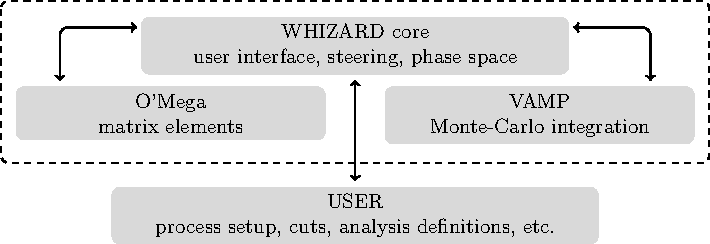
\includegraphics[width=0.9\textwidth]{whizstruct}  
  \caption{General structure of the \whizard\ package.} 
\end{figure}
discussed, while the next sections are devoted to the setup and
compilation of code for particular processes, the specification of
beams, beam structure and polarization. The next step is the
integration, controlling the integration, phase space, generator cuts,
scales and weights, proceeding further to event generation and
decays. At the end of this chapter, \whizard's internal data analysis
methods and graphical visualization options are documented. 

The following chapters are dedicated to the physics implemented in
\whizard: methods for hard matrix interactions in
Chap.~\ref{chap:hardint}. Then, in Chap.~\ref{chap:physics},
implemented methods for adaptive multi-channel integration,
particularly the integrator \vamp\ are explained, together with the
algorithms for the generation of the phase-space in \whizard. Finally,
an overview is given over the physics models implemented in \whizard\
and its matrix element generator \oMega, together with possibilities
for their extension. After that, the next chapter discusses parton
showering, matching and hadronization as well as options for event
normalizations and supported event formats. Also weighted event
generation is explained along the lines with options for negative
weights. Then, in Chap.~\ref{chap:user}, options for user to plug-in
self-written code into the \whizard\ framework are detailed, e.g. for
observables, selections and cut functions, or for spectra and
structure functions. Also, static executables are discussed. 

Chap.~\ref{chap:visualization} is a stand-alone documentation of
GAMELAN, the interal graphics support for the visualization of data
and analysis. The next chapter, Chap.~\ref{chap:userint} details user
interfaces: how to use more options of the \whizard\ command on the
command line, how to use \whizard\ interactively, and how to include
\whizard\ as a library into the user's own program. 

Then, an extensive list of examples in Chap.~\ref{chap:examples}
documenting physics examples from the LEP, SLC, HERA, Tevatron, and
LHC colliders to future linear and circular colliders. This chapter is
a particular good reference for the beginning, as the whole chain from
choosing a model, setting up processes, the beam structure, the
integration, and finally simulation and (graphical) analysis are
explained in detail. 

More technical details about efficiency, tuning and advance usage of
\whizard\ are collected in Chap.~\ref{chap:tuning}. Then,
Chap.~\ref{chap:extmodels} shows how to set up your own new physics
model with the help of external programs like \sarah\ or
\FeynRules\ program and include it into the \whizard\ event
generator.  

In the appendices, we e.g. give an exhaustive reference list of
SINDARIN commands and built-in variables. 

Please report any inconsistencies, bugs, problems or simply pose open
questions to our contact \url{whizard@desy.de}.


%%%%%

\section{Historical remarks}

This section gives a historical overview over the development of
\whizard\ and can be easily skipped in a (first) reading of the
manual. \whizard\ has been developed in a first place as a tool for
the physics at the then planned linear electron-positron collider
TESLA around 1999. The intention was to have a tool at hand to
describe electroweak physics of multiple weak bosons and the Higgs
boson as precise as possible with full matrix elements. Hence, the
acronym: \ttt{WHiZard}, which stood for $\mathbf{W}$, {\bf H}iggs,
$\mathbf{Z}$, {\bf a}nd {\bf r}espective {\bf d}ecays. 

Several components of the \whizard\ package that are also available as
independent sub-packages have been published already before the first
versions of the \whizard\ generator itself: the multi-channel adaptive
Monte-Carlo integration package \vamp\ has been released mid
1998~\cite{VAMP}. The dedicated packages for the simulation of linear
lepton collider beamstrahlung and the option for a photon collider on
Compton backscattering (\ttt{CIRCE1/2}) date back even to mid
1996~\cite{CIRCE}. Also parts of the code for \whizard's internal
graphical analysis (the \gamelan\ module) came into existence already
around 1998. 

After first inofficial versions, the official version 1 of \whizard\
was release in the year 2000. The development, improvement and
incorporation of new features continued for roughly a decade. Major
milestones in the development were the full support of all kinds of
beyond the Standard Model (BSM) models including spin 3/2 and spin 2
particles and the inclusion of the MSSM, the NMSSM, Little Higgs
models and models for anomalous couplings as well as extra-dimensional
models from version 1.90 on. In the beginning, several methods for
matrix elements have been used, until the in-house matrix element
generator \oMega\ became available from version 1.20 on. It was
included as a part of the \whizard\ package from version 1.90 on. The
support for full color amplitudes came with version 1.50, but in a
full-fledged version from 2.0 on. Version 1.40 brought the necessary
setups for all kinds of collider environments, i.e. asymmetric beams,
decay processes, and intrinsic $p_T$ in structure functions. 

Version 2.0 was released in April 2010 as an almost complete rewriting
of the original code. It brought the construction of an internal
density-matrix formalism which allowed the use of factorized
production and (cascade) decay processes including complete color and
spin correlations. Another big new feature was the command-line
language SINDARIN for steering all parts of the program. Also, many
performance improvement have taken place in the new release series,
like OpenMP parallelization, speed gain in matrix element generation
etc. Version 2.2 came out in May 2014 as a major refactoring of the
program internals but keeping (almost everywhere) the same user
interface. New features are inclusive processes, reweighting, and more
interfaces for QCD environments (BLHA/HOPPET).

The following tables shows some of the major steps (physics
implementation and/or technical improvements) in the development
of \whizard:

\begin{center}
\begin{tabular}{|l|l|l|}\hline
  0.99 & 08/1999 & Beta version \\\hline
  1.00 & 12/2000 & First public version \\\hline
  1.10 & 03/2001 & Libraries; \pythiasix\ interface \\ 
  1.11 & 04/2001 & PDF support; anomalous couplings \\ \hline
  1.20 & 02/2002 & \oMega\ matrix elements; \ttt{CIRCE} support\\
  1.22 & 03/2002 & QED ISR; beam remnants, phase space improvements \\
  1.25 & 05/2003 & MSSM; weighted events; user-code plug-in \\
  1.28 & 04/2004 & Improved phase space; SLHA interface; signal catching
  \\\hline
  1.30 & 09/2004 & Major technical overhaul \\\hline
  1.40 & 12/2004 & Asymmetric beams; decays; $p_T$ in structure 
  functions \\\hline
  1.50 & 02/2006 & QCD support in \oMega\ (color flows); LHA format \\
  1.51 & 06/2006 & $Hgg$, $H\gamma\gamma$; Spin 3/2 + 2; BSM models
  \\\hline
  1.90 & 11/2007 & \oMega\ included; LHAPDF support; $Z'$; $WW$ scattering \\ 
  1.92 & 03/2008 & LHE format; UED; parton shower beta version \\ 
  1.93 & 04/2009 & NMSSM; SLHA2 accord; improved color/flavor sums \\
  1.95 & 02/2010 & MLM matching; development stop in version 1
  \\
  1.97 & 05/2011 & Manual for version 1 completed. \\\hline\hline
  2.0.0 & 04/2010 & Major refactoring: automake setup; dynamic
  libraries \\ 
  & & improved speed; cascades; OpenMP; SINDARIN steering language \\
  2.0.3 & 07/2010 & QCD ISR+FSR shower; polarized beams \\ 
  2.0.5 & 05/2011 & Builtin PDFs; static builds; relocation scripts \\
  2.0.6 & 12/2011 & Anomalous top couplings; unit tests \\\hline
  2.1.0 & 06/2012 & Analytic ISR+FSR parton shower; anomalous Higgs
  couplings \\\hline
  2.2.0 & 05/2014 & Major technical refactoring: abstract
  object-orientation; 2HDM; \\
  & & reweighting; LHE v2/3; BLHA; HOPPET interface; inclusive
  processes \\
  2.2.1 & 05/2014 & CJ12 PDFs; FastJet interface \\
  2.2.2 & 07/2014 & LHAPDF6 support; correlated LC beams; GuineaPig
  interface \\
  2.2.3 & 11/2014 & O'Mega virtual machine; lepton collider top
  pair threshold; Higgs singlet extension \\
  2.2.4 & 02/2015 & LCIO support; progress on NLO; many technical
  bug fixes \\
  2.2.7 & 08/2015 & progress on POWHEG; fixed-order NLO events;
  revalidation of ILC event chain \\ 
  2.2.8 & 11/2015 & support for quadruple precision; StdHEP included;
  SM dim 6 operators supported
  \\\hline 
\end{tabular}
\end{center}

\vspace{.5cm}

For a detailed overview over the historical development of the code
confer the \ttt{ChangeLog} file and the commit messages in our
revision control system repository. 

%%%%%

\section{About examples in this manual}

Although \whizard\ has been designed as a Monte Carlo event generator
for LHC physics, several elementary steps and aspects of its usage
throughout the manual will be demonstrated with the famous textbook
example of $e^+e^- \to \mu^+ \mu^-$. This is the same process, the
textbook by Peskin/Schroeder \cite{PeskinSchroeder} uses as a prime
example to teach the basics of quantum field theory. We use this
example not because it is very special for \whizard\ or at the time
being a relevant physics case, but simply because it is the easiest
fundamental field theoretic process without the complications of
structured beams (which can nevertheless be switched on like for ISR
and beamstrahlung!), the need for jet definitions/algorithms and
flavor sums; furthermore, it easily accomplishes a demonstration of
polarized beams. After the basics of \whizard\ usage have been
explained, we move on to actual physics cases from LHC (or Tevatron). 


\newpage
\chapter{Installation}
\label{chap:installation}

\section{Package Structure}

\whizard\ is a software package that consists of a main executable
program (which is called \ttt{whizard}), libraries, auxiliary
executable programs, and machine-independent data files.  The whole
package can be installed by the system administrator, by default, on a
central location in the file system (\ttt{/usr/local} with its proper
subdirectories).  Alternatively, it is possible to install it in a
user's home directory, without administrator privileges, or at any
other location.

A \whizard\ run requires a workspace, i.e., a writable directory where
it can put generated code and data.  There are no constraints on the
location of this directory, but we recommend to use a separate
directory for each \whizard\ project, or even for each \whizard\ run.

Since \whizard\ generates the matrix elements for scattering and decay
processes in form of \fortran\ code that is automatically compiled and
dynamically linked into the running program, it requires a working
\fortran\ compiler not just for the installation, but also at runtime.

The previous major version \whizard1 did put more constraints on the
setup.  In a nutshell, not just the matrix element code was compiled
at runtime, but other parts of the program as well, so the whole
package was interleaved and had to be installed in user space.  The
workflow was controlled by \ttt{make} and PERL scripts.  These
constraints are gone in the present version in favor of a clean
separation of installation and runtime workspace.


\section{\label{sec:prerequisites}Prerequisites}

\subsection{No Binary Distribution}

\whizard\ is currently not distributed as a binary package, nor is it
available as a debian or RPM package.  This might change in the
future.  However, compiling from source is very simple (see below).
Since the package needs a compiler also at runtime, it would not work
without some development tools installed on the machine, anyway. 

Note, however, that we support an install script, that downloads all
necessary prerequisites, and does the configuration and compilation
described below automatically. This is called the ``instant WHIZARD''
and is accessible through the WHIZARD webpage from version 2.1.1 on:
\url{http://whizard.hepforge.org/versions/install/install-whizard-2.X.X.sh}.
Download this shell script, make it executable by
\begin{interaction}
  chmod +x install-whizard-2.X.X.sh
\end{interaction}
and execute it. Note that this also involves compilation of the
required \ttt{Fortran} compiler which takes 1-3 hours depending on
your system.
\ttt{Darwin} operating systems (a.k.a. as \ttt{Mac OS X}) have a very
similar general system for all sorts of software, called
\ttt{MacPorts} (\url{http://www.macports.org}). This offers to install
\whizard\ as one of its software ports, and is very similar to
``instant WHIZARD'' described above. 


\subsection{Tarball Distribution}

This is the recommended way of obtaining \whizard.  You may download
the current stable distribution from the \whizard\ webpage, 
hosted at the HepForge webpage
\begin{quote}
  \hepforgepage
\end{quote}
The distribution is a single file, say \ttt{whizard-\thisversion.tgz} for
version \thisversion.

You need the additional prerequisites:
\begin{itemize}
\item
  GNU \ttt{tar} (or \ttt{gunzip} and \ttt{tar}) for unpacking the
  tarball.
\item
  The \ttt{make} utility.  Other standard Unix utilities (\ttt{sed},
  \ttt{grep}, etc.) are usually installed by default.
\item
  A modern \fortran\ compiler (see Sec.~\ref{sec:compilers} for
  details).
\item
  The \ocaml\ system.  \ocaml\ is a functional and object-oriented
  language.  Version 3.12 or later is required to compile all components 
  of \whizard. The package is freely available either as a debian/RPM package
  on your system (it might be necessary to install it from the usual
  repositories), or you can obtain it directly from
  \begin{quote}
    \url{http://caml.inria.fr}
  \end{quote}
  and install it yourself.  If desired, the package can be installed
  in user space without administrator privileges\footnote{
    Unfortunately, the version of the \ocaml\
    compiler from 3.12.0 broke backwards compatibility. Therefore, 
    versions of \oMega/\whizard\ up to 2.0.2 only compile with older
    versions (3.11.x works). This has been fixed in versions 
    2.0.3 and later. See also Sec.~\ref{sec:buildproblems}.}.
\end{itemize}
The following optional external packages are not required, but used
for certain purposes.  Make sure to check whether you will need any of
them, before you install \whizard.
\begin{itemize}
\item
  \LaTeX\ and \metapost\ for data visualization.  Both are part of the
  \TeX\ program family.  These programs are not absolutely necessary,
  but \whizard\ will lack the tools for visualization without them.
\item
  The \lhapdf\ structure-function library.  See
  Sec.~\ref{sec:lhapdf_install}.
\item
  The \hoppet\ structure-function matching tool. See 
  Sec.~\ref{sec:hoppet}.
\item
  The \hepmc\ event-format package.  See Sec.~\ref{sec:hepmc}.
\item
  The \fastjet\ jet-algorithm package.  See Sec.~\ref{sec:fastjet}.
\item
  The \lcio\ event-format package.  See Sec.~\ref{sec:lcio}.
\end{itemize}
Until version v2.2.7 of \whizard, the event-format package \stdhep\ used
to be available as an external package. As their distribution is frozen
with the final version v5.06.01, and it used to be notoriously difficult to
compile and link \stdhep\ into \whizard, it was decided to include \stdhep\
into \whizard. This is the case from version v2.2.8 of \whizard\ on. Linking
against an external version of \stdhep\ is precluded from there
on. Nevertheless, we list some explanations in Sec.~\ref{sec:stdhep}. 
Once these prerequisites are met, you may unpack the package in a
directory of your choice
\begin{quote}\small\tt
  some-directory> tar xzf whizard-\thisversion.tgz
\end{quote}
and proceed.\footnote{Without GNU \ttt{tar}, this would read
  \ttt{\small gunzip -c whizard-\thisversion.tgz | tar xz -}} 

For using external physics models that are directly supported by
\whizard\ and \oMega, the user can use tools like \sarah\ or
\FeynRules. There installation and linking to \whizard\ will be
explained in Chap.~\ref{chap:extmodels}.

The directory will then contain a subdirectory \ttt{whizard-\thisversion}
where the complete source tree is located.  To update later to a new
version, repeat these steps.  Each new version will unpack in a
separate directory with the appropriate name.


\subsection{SVN Repository Version}

If you want to install the latest development version, you have to
check it out from the \whizard\ SVN repository.

In addition to the prerequisites listed in the previous section, you
need:
\begin{itemize}
\item
  The \ttt{subversion} package (\ttt{svn}), the tool for dealing with
  SVN repositories.
\item
  The \ttt{autoconf} package, part of the \ttt{autotools} development
  system.
\item
  The \ttt{noweb} package, a light-weight tool for literate programming.  This
  package is nowadays often part of Linux distributions\footnote{In
    Ubuntu from version 10.04 on, and in Debian since
    squeeze. For \ttt{Mac OS X}, \ttt{noweb} is available via the
    \ttt{MacPorts} system.}.  You can obtain the source code
  from\footnote{Please, do not use any of the binary builds from this
    webpage. Probably all of them are quite old and broken.}  
  \begin{quote}
    \url{http://www.cs.tufts.edu/~nr/noweb/}
  \end{quote}
\end{itemize}
To start, go to a directory of your choice and execute
\begin{interaction}
  your-src-directory> svn checkout http://whizard.hepforge.org/svn/trunk/ .
\end{interaction}
The SVN source tree will appear in the current directory.  To update
later, you just have to execute
\begin{interaction}
  your-src-directory> svn update
\end{interaction}
within that directory.

After checking out the sources, run\footnote{At least, version 2.65 of
  the \ttt{autoconf} package is required.}
\begin{interaction}
  your-src-directory> autoreconf
\end{interaction}
This will generate a \ttt{configure} script.


\subsection{\label{sec:compilers}Fortran Compilers}

\whizard\ is written in modern \fortran.  To be precise, it uses a
subset of the \fortranOThree\ standard.  At the time of this writing,
this subset is supported by, at least, the following compilers:
\begin{itemize}
\item
  \ttt{gfortran} (GNU, Open Source).  You will need version 4.7.4
  or higher\footnote{Note that \whizard\ versions 2.0.0 until 2.1.1 compiled
  with \ttt{gfortran} 4.5.x and 4.6.x, but the object-oriented
  refactoring of the \whizard\ code from 2.2 on made a switch to
  \ttt{gfortran} 4.7.4 or higher necessary. \ttt{gcc} 4.7.0 contains a
  major bug in the static \ttt{libstdc++} library which prevented
  static builds of \whizard\ with external \ttt{C++} libraries.}.
  \ttt{gcc} 4.7.1-3 suffer from too many bugs in the object-orientation.
\item
  \ttt{nagfor} (NAG).  You will need version 5.2 or higher.
\item
  \ttt{ifort} (Intel). You will need version 16.0.0 or higher. In
  order to be sure that everything works properly, use
  \ttt{FCFLAGS=-standard-semantics}.  
\end{itemize}
There are some commercial compilers that might be able to compile
\whizard\ 2.2 in the near future, but at the time of writing, all of
the compilers listed below contained compiler bugs. Consult the
\whizard\ website for updates on this situation. 
\begin{itemize}
\item
  \ttt{pgfortran} (PGI).  You will need a more modern version than
  15.10.
\item{ekopath}. You will need a more modern version than 4.0.  
\end{itemize}

%%%%%

\subsection{LHAPDF}
\label{sec:lhapdf_install}

For computing scattering processes at hadron colliders such as the
LHC, \whizard\ has a small set of standard structure-function
parameterizations built in, cf.\ Sec.~\ref{sec:built-in-pdf}.  For
many applications, this will be sufficient, and you can skip this
section.

However, if you need structure-function parameterizations that are not
in the default set (e.g. PDF error sets), you can use the \lhapdf\
structure-function library, which is an external package.  It has to
be linked during \whizard\ installation.  For use with \whizard,
version 5.3.0 or higher of the library is required\footnote{ Note that
  PDF sets which contain photons as partons are only supported with
  \whizard\ for \lhapdf\ version 5.7.1 or higher}. The \lhapdf\
package has undergone a major rewriting from \fortran\ version 5
to \ttt{C++} version 6. While still maintaining the interface for
the \lhapdf\ version 5 series, from version 2.2.2 of \whizard\ on, the
new release series of \lhapdf, version 6.0 and higher, is also
supported.  

If \lhapdf\ is not yet installed on your system, you can download it from
\begin{quote}
  \url{http://lhapdf.hepforge.org}
\end{quote}
for the most recent LHAPDF version 6 and newer, or
\begin{quote}
  \url{http://lhapdf.hepforge.org/lhapdf5}
\end{quote}
for version 5 and older, and install it.  The website contains
comprehensive documentation on the configuring and installation
procedure.  Make sure that you have downloaded and installed not just
the package, but also the data sets. Note that \lhapdf\ version 5
needs both a \fortran\ and a \ttt{C++} compiler. 

During \whizard\ configuration, \whizard\ looks for the script
\ttt{lhapdf} (which is present in \lhapdf\ series 6) first, and then
for \ttt{lhapdf-config} (which is present since \lhapdf\ version
4.1.0): if those are in an executable path (or only 
the latter for \lhapdf\ version 5), the environment variables for
\lhapdf\ are automatically recognized by \whizard, as well as the
version number. This should look like this in the \ttt{configure}
output (for \lhapdf\ version 6 or newer),

\begin{footnotesize}
\begin{verbatim}
   configure: --------------------------------------------------------------
   configure: --- LHAPDF ---
   configure:
   checking for lhapdf... /usr/local/bin/lhapdf
   checking for lhapdf-config... /usr/local/bin/lhapdf-config
   checking the LHAPDF version... 6.1.3
   checking the major version... 6
   checking the LHAPDF pdfsets path... /usr/local/share/LHAPDF
   checking the standard PDF sets...  all standard PDF sets installed
   checking if LHAPDF is functional (may take a while)... yes
   checking LHAPDF... yes
   configure: --------------------------------------------------------------
\end{verbatim}
\end{footnotesize}
while for \lhapdf\ version 5 and older it looks like this:

\begin{footnotesize}
\begin{verbatim}
   configure: --------------------------------------------------------------
   configure: --- LHAPDF ---
   configure: 
   checking for lhapdf... no
   checking for lhapdf-config... /usr/local/bin/lhapdf-config
   checking the LHAPDF version... 5.9.1
   checking the major version... 5
   checking the LHAPDF pdfsets path... /usr/local/share/lhapdf/PDFsets
   checking the standard PDF sets...  all standard PDF sets installed
   checking for getxminm in -lLHAPDF... yes
   checking for has_photon in -lLHAPDF... yes
   configure: --------------------------------------------------------------
\end{verbatim}
\end{footnotesize}

If you want to use a different \lhapdf\ (e.g. because the one installed
on your system by default is an older one), the preferred way to do so
is to put the \ttt{lhapdf} (and/or \ttt{lhapdf-config}) scripts in an
executable path that is checked before the system paths,
e.g. \ttt{<home>/bin}.  

For the old series, \lhapdf\ version 5, a possible error could arise
if \lhapdf\ had been compiled with a different \fortran\ compiler than
\whizard, and if the run-time library of that \fortran\ compiler had
not been included in the \whizard\ configure process. The output then
looks like this: 

\begin{footnotesize}
\begin{verbatim}
   configure: --------------------------------------------------------------
   configure: --- LHAPDF ---
   configure:
   checking for lhapdf... no
   checking for lhapdf-config... /usr/local/bin/lhapdf-config
   checking the LHAPDF version... 5.9.1
   checking the major version... 5
   checking the LHAPDF pdfsets path... /usr/local/share/lhapdf/PDFsets
   checking for standard PDF sets... all standard PDF sets installed
   checking for getxminm in -lLHAPDF... no
   checking for has_photon in -lLHAPDF... no
   configure: --------------------------------------------------------------
\end{verbatim}
\end{footnotesize}

So, the \whizard\ configure found the \lhapdf\ distribution, but could
not link because it could not resolve the symbols inside the
library. In case of failure, for more details confer the
\ttt{config.log}. 

If \lhapdf\ is installed in a non-default directory where
\whizard\ would not find it, set the environment variable
\ttt{LHAPDF\_DIR} to the correct installation path when configuring
\whizard.

The check for the standard PDF sets are those sets that are used in
the default \whizard\ self tests in the case \lhapdf\ is enabled and 
correctly linked. If some of them are missing, then this test will
result in a failure. They are the \ttt{CT10} set for \lhapdf\ version
6 (for version 5, \ttt{cteq61.LHpdf}, \ttt{cteq6ll.LHpdf},
\ttt{cteq5l.LHgrid}, and \ttt{GSG961.LHgrid} are demanded). If you
want to use \lhapdf\ inside \whizard\ please install them such that
\whizard\ could perform all its sanity checks with them. The last
check is for the \ttt{has\_photon} flag, which tests whether photon
PDFs are available in the found \lhapdf\ installation. 

%%%%%

\subsection{HOPPET}
\label{sec:hoppet}

\hoppet\ (not Hobbit) is a tool for the QCD DGLAP evolution of PDFs
for hadron colliders. It provides possibilities for matching
algorithms for 4- and 5-flavor schemes, that are important for
precision simulations of $b$-parton initiated processes at hadron
colliders. If you are not interested in those features, you can skip
this section. Note that this feature is not enabled by default (unlike
e.g. \lhapdf), but has to be explicitly during the configuration
(see below):
\begin{interaction}
  your-build-directory> your-src-directory/configure --enable-hoppet
\end{interaction}
If you \ttt{configure} messages like the following:
\begin{footnotesize}
\begin{verbatim}
configure: --------------------------------------------------------------
configure: --- HOPPET ---
configure: 
checking for hoppet-config... /usr/local/bin/hoppet-config
checking for hoppetAssign in -lhoppet_v1... yes
configure: --------------------------------------------------------------
\end{verbatim}
\end{footnotesize}
then you know that \hoppet\ has been found and was correctly
linked. If that is not the case, you have to specify the location of
the \hoppet\ library, e.g. by adding 
\begin{interaction}
  HOPPET=<hoppet\_directory>/lib
\end{interaction}
to the \ttt{configure} options above. For more details, please confer
the \hoppet\ manual.

%%%%%

\subsection{HepMC}
\label{sec:hepmc}

\hepmc\ is a \ttt{C++} class library for handling collider scattering
events.  In particular, it provides a portable format for event files.
If you want to use this format, you should link \whizard\ with \hepmc,
otherwise you can skip this section.

If it is not already installed on your system, you may obtain
\hepmc\ from one of these two webpages:
\begin{quote}
  \url{http://lcgapp.cern.ch/project/simu/HepMC/}
\end{quote}
or 
\begin{quote}
  \url{https://sft.its.cern.ch/jira/browse/HEPMC}
\end{quote}
If the \hepmc\ library is linked with the installation, \whizard\ is
able to read and write files in the \hepmc\ format.

Detailed information on the installation and usage can be found on the
\hepmc\ homepage. We give here only some brief details relevant for
the usage with \whizard: For the compilation of HepMC one needs a
\ttt{C++} compiler. Then the procedure is the same as for the
\whizard\ package, namely configure HepMC: 
\begin{interaction}
  configure --with-momentum=GEV --with-length=MM --prefix=<install dir> 
\end{interaction}
Note that the particle momentum and decay length flags are mandatory, and
we highly recommend to set them to the values \ttt{GEV} and \ttt{MM},
respectively. After configuration, do \ttt{make}, an optional
\ttt{make check} (which might sometimes fail for non-standard values
of momentum and length), and finally \ttt{make install}.

A \whizard\ configuration for HepMC looks like this:
\begin{footnotesize}
  \begin{verbatim}
   configure: --------------------------------------------------------------
   configure: --- HepMC ---
   configure:
   checking the HepMC version... 2.06.09
   checking for GenEvent class in -lHepMC... yes
   configure: --------------------------------------------------------------    
  \end{verbatim}
\end{footnotesize}

If \hepmc\ is installed in a non-default directory where \whizard\
would not find it, set the environment variable \ttt{HEPMC\_DIR} to
the correct installation path when configuring \whizard.  Furthermore,
the environment variable \ttt{CXXFLAGS} allows you to set specific
\ttt{C/C++} preprocessor flags, e.g. non-standard include paths for
header files.

%%%%%

\subsection{PYTHIA8}
\label{sec:pythia8}

\emph{NOTE: This is at the moment not yet supported, but merely a stub 
with the only purpose to be recognized by the build system.}

\pythiaeight\ is a \ttt{C++} class library for handling hadronization,
showering and underlying event. If you want to use this feature (once it is
fully supported in \whizard), you should link \whizard\ with \pythiaeight,
otherwise you can skip this section.

If it is not already installed on your system, you may obtain
\pythiaeight\ from
\begin{quote}
  \url{http://home.thep.lu.se/~torbjorn/Pythia.html}
\end{quote}
If the \pythiaeight\ library is linked with the installation, \whizard\ will
be able to use its hadronization and showering, once this is fully supported
within \whizard.

To link a \pythiaeight\ installation to \whizard, you should specify the flag
\begin{quote}
\ttt{--enable-pythia8}
\end{quote}
to \ttt{configure}.  If  \pythiaeight\ is installed in a non-default directory 
where \whizard\ would not find it, specify also
\begin{quote}
\ttt{--with-pythia8=\emph{<your-pythia8-installation-path>}}
\end{quote}

A successful \whizard\ configuration should produce a screen output
similar to this:
\begin{footnotesize}
\begin{verbatim}
configure: --------------------------------------------------------------
configure: --- SHOWERS PYTHIA6 PYTHIA8 MPI ---
configure: 
[....]
checking for pythia8-config... /usr/local/bin/pythia8-config
checking if PYTHIA8 is functional... yes
checking PYTHIA8... yes
configure: WARNING: PYTHIA8 configure is for testing purposes at the moment.
configure: --------------------------------------------------------------
\end{verbatim}
\end{footnotesize}

%%%%%

\subsection{FastJet}
\label{sec:fastjet}

\emph{NOTE: This is an experimental feature.}

\fastjet\ is a \ttt{C++} class library for handling jet clustering.
If you want to use this feature, you should link \whizard\ with \fastjet,
otherwise you can skip this section.

If it is not already installed on your system, you may obtain
\fastjet\ from
\begin{quote}
  \url{http://fastjet.fr}
\end{quote}
If the \fastjet\ library is linked with the installation, \whizard\ is
able to call the jet algorithms provided by this program for the purposes of
applying cuts and analysis.

To link a \fastjet\ installation to \whizard, you should specify the flag
\begin{quote}
\ttt{--enable-fastjet}
\end{quote}
to \ttt{configure}.  If  \fastjet\ is installed in a non-default directory
where \whizard\ would not find it, specify also
\begin{quote}
\ttt{--with-fastjet=\emph{<your-fastjet-installation-path>}}
\end{quote}

A successful \whizard\ configuration should produce a screen output
similar to this:
\begin{footnotesize}
\begin{verbatim}
configure: --------------------------------------------------------------
configure: --- FASTJET ---
configure: 
checking for fastjet-config... /usr/local/bin/fastjet-config
checking if FastJet is functional... yes
checking FastJet... yes
configure: --------------------------------------------------------------
\end{verbatim}
\end{footnotesize}

%%%%%

\subsection{STDHEP}
\label{sec:stdhep}

\stdhep\ is a  library for handling collider scattering
events~\cite{stdhep}.  In particular, it provides a portable format
for event files. Until version 2.2.7 of \whizard, \stdhep\ that was
maintained by Fermilab, could be linked as an externally compiled
library. As the \stdhep\ package is frozen in its final release
v5.06.1 and no longer maintained, it has from version 2.2.8 been
included \whizard. This eases many things, as it was notoriously
difficult to compile and link \stdhep\ in a way compatible with
\whizard. Not the full package has been included, but only the
libraries for file I/O (\texttt{mcfio}, the library for the XDR
conversion), while the various translation tools for \pythia, \herwig,
etc.  have been abandoned. Note that \stdhep\ has largely been
replaced in the hadron collider community by the \hepmc\ format, and
in the lepton collider community by \lcio. \whizard\ might serve as a
conversion tools for all these formats, but other tools also exist, of
course. 

If the \stdhep\ library is linked with the installation, \whizard\ is 
able to write files in the \stdhep\ format, the  corresponding
configure output notifies you that \stdhep\ is always included:
\begin{footnotesize}
\begin{verbatim}
configure: --------------------------------------------------------------
configure: --- STDHEP ---
configure:
configure: StdHEP v5.06.01 is included internally
configure: -------------------------------------------------------------- 
\end{verbatim}
\end{footnotesize}

%%%%%

\subsection{LCIO}
\label{sec:lcio}


\lcio\ is a \ttt{C++} class library for handling collider scattering
events.  In particular, it provides a portable format for event files.
If you want to use this format, you should link \whizard\ with \lcio,
otherwise you can skip this section.

If it is not already installed on your system, you may obtain
\lcio\ from:
\begin{quote}
  \url{http://lcio.desy.de}
\end{quote}
or 
\begin{quote}
  \url{https://sft.its.cern.ch/jira/browse/HEPMC}
\end{quote}
If the \hepmc\ library is linked with the installation, \whizard\ is
able to read and write files in the \hepmc\ format.

Detailed information on the installation and usage can be found on the
\hepmc\ homepage. We give here only some brief details relevant for
the usage with \whizard: For the compilation of HepMC one needs a
\ttt{C++} compiler. Then the procedure is the same as for the
\whizard\ package, namely configure HepMC: 
\begin{interaction}
  configure --with-momentum=GEV --with-length=MM --prefix=<install dir> 
\end{interaction}
Note that the particle momentum and decay length flags are mandatory, and
we highly recommend to set them to the values \ttt{GEV} and \ttt{MM},
respectively. After configuration, do \ttt{make}, an optional
\ttt{make check} (which might sometimes fail for non-standard values
of momentum and length), and finally \ttt{make install}.

A \whizard\ configuration for \lcio\ looks like this:
\begin{footnotesize}
  \begin{verbatim}
   configure: --------------------------------------------------------------
   configure: --- LCIO ---
   configure:
   checking the LCIO version... 2.4.2
   checking for LCEventImpl class in -llcio... yes
   configure: --------------------------------------------------------------    
  \end{verbatim}
\end{footnotesize}

If \lcio\ is installed in a non-default directory where \whizard\
would not find it, set the environment variable \ttt{LCIO\_DIR} to
the correct installation path when configuring \whizard.  Furthermore,
the environment variable \ttt{CXXFLAGS} allows you to set specific
\ttt{C/C++} preprocessor flags, e.g. non-standard include paths for
header files.

{\bf Installation bug of \lcio:} when using \texttt{cmake}
\texttt{v3}, it is (at least with most known \lcio\ versions) not
possible to specify the installation path. Instead, files are
installed into the source directory of \lcio. So the binaries in
\texttt{bin}, the libraries in \texttt{lib}, and the headers in
\texttt{include} have to be copied by hand to the desired
\texttt{prefix}. 


%%%%%

\section{Installation}
\label{sec:installation}

Once you have unpacked the source (either the tarball or the SVN
version), you are ready to compile it.  There are several options.


\subsection{Central Installation}
This is the default and recommended way, but it requires adminstrator
privileges.  Make sure that all
prerequisites are met (Sec.~\ref{sec:prerequisites}).
\begin{enumerate}
\item
  Create a fresh directory for the \whizard\ build.  It is recommended
  to keep this separate from the source directory.
\item
  Go to that directory and execute
  \begin{interaction}
    your-build-directory> your-src-directory/configure
  \end{interaction}
  This will analyze your system and prepare the compilation of \whizard\
  in the build directory.  Make sure to set the proper options to
  \ttt{configure}, see Sec.~\ref{sec:configure-options} below.
\item
  Call \ttt{make} to compile and link \whizard:
  \begin{interaction}
    your-build-directory> make
  \end{interaction}
\item
  If you want to make sure that everything works, run
  \begin{interaction}
    your-build-directory> make check
  \end{interaction}
  This will take some more time.
\item
  Become superuser and say
  \begin{interaction}
    your-build-directory> make install
  \end{interaction}
\end{enumerate}
\whizard\ should now installed in the default locations, and the
executable should be available in the standard path.  Try to call
\ttt{whizard --help} in order to check this.

\subsection{Installation in User Space}
You may lack administrator privileges on your system.  In that case,
you can still install and run \whizard.  Make sure that all
prerequisites are met (Sec.~\ref{sec:prerequisites}).
\begin{enumerate}
\item
  Create a fresh directory for the \whizard\ build.  It is recommended
  to keep this separate from the source directory.
\item
  Reserve a directory in user space for the \whizard\ installation.
  It should be empty, or yet non-existent.
\item
  Go to that directory and execute
  \begin{interaction}
    your-build-directory> your-src-directory/configure 
                               --prefix=your-install-directory
  \end{interaction}
  This will analyze your system and prepare the compilation of \whizard\
  in the build directory.  Make sure to set the proper additional options to
  \ttt{configure}, see Sec.~\ref{sec:configure-options} below.
\item
  Call \ttt{make} to compile and link \whizard:
  \begin{interaction}
    your-build-directory> make
  \end{interaction}
\item
  If you want to make sure that everything works, run
  \begin{interaction}
    your-build-directory> make check
  \end{interaction}
  This will take some more time.
\item
  Install:
  \begin{interaction}
    your-build-directory> make install
  \end{interaction}
\end{enumerate}
\whizard\ should now be installed in the installation directory of your
choice.  If the installation is not in your standard search paths, you
have to account for this by extending the paths appropriately, see
Sec.~\ref{sec:workspace}.


\subsection{Configure Options}
\label{sec:configure-options}

The configure script accepts environment variables and flags.  They
can be given as arguments to the \ttt{configure} program in arbitrary
order.  You may run \ttt{configure --help} for a listing; only the
last part of this long listing is specific for the \whizard\ system.
Here is an example:
\begin{interaction}
  configure  FC=gfortran-4.8  FCFLAGS="-g -O3"  --enable-fc-openmp
\end{interaction}

The most important options are
\begin{itemize}
\item
  \ttt{FC} (variable): The \fortran\ compiler.  This is necessary if
  you need a compiler different from the standard compiler on the
  system, e.g., if the latter is too old.
\item
  \ttt{FCFLAGS} (variable): The flags to be given to the Fortran
  compiler.  The main use is to control the level of optimization.
\item
  \ttt{--prefix=\var{directory-name}}: Specify a non-default directory
  for installation.
\item
  \ttt{--enable-fc-openmp}: Enable parallel executing via OpenMP on a
  multi-processor/multi-core machine.  This works only if OpenMP is
  supported by the compiler (e.g., \ttt{gfortran}).  When running
  \whizard, the number of processors that are actually requested can
  be controlled by the user.  Without this option, \whizard\ will run
  in serial mode on a single core.  See Sec.~\ref{sec:openmp} for
  further details.
\item
  \ttt{LHADPF\_DIR} (variable): The location of the optional \lhapdf\
  package, if non-default.
\item
  \ttt{HOPPET\_DIR} (variable): The location of the optional \hoppet\
  package, if non-default.
\item
  \ttt{HEPMC\_DIR} (variable): The location of the optional \hepmc\ package, if
  non-default.
\item
  \ttt{LCIO\_DIR} (variable): The location of the optional \lcio\
  package, if non-default.
\end{itemize}

Other flags that might help to work around possible problems are the
flags for the $C$ and $C++$ compilers as well as the \ttt{Fortran77}
compiler, or the linker flags and additional libraries for the linking
process. 
\begin{itemize}
\item 
  \ttt{CC} (variable): \ttt{C} compiler command
\item
  \ttt{F77} (variable): \ttt{Fortran77} compiler command
\item
  \ttt{CXX} (variable): \ttt{C++} compiler command
\item
  \ttt{CPP} (variable): \ttt{C} preprocessor
\item
  \ttt{CXXCPP} (variable): \ttt{C++} preprocessor
\item
  \ttt{CFLAGS} (variable): \ttt{C} compiler flags
\item
  \ttt{FFLAGS} (variable): \ttt{Fortran77} compiler flags
\item
  \ttt{CXXFLAGS} (variable): \ttt{C++} compiler flags
\item
  \ttt{LIBS} (variable): libraries to be passed to the linker as
  \ttt{-l{\em library}}
\item
  \ttt{LDFLAGS} (variable): non-standard linker flags
\end{itemize}

For other options (like e.g. \ttt{--with-precision=...} etc.) please
see the \ttt{configure --help} option.

%%%%%

\subsection{Details on the Configure Process}

The configure process checks for the build and host system type; only
if this is not detected automatically, the user would have to specify
this by himself. After that system-dependent files are searched for,
LaTeX and Acroread for documentation and plots, the \fortran\ compiler 
is checked, and finally the \ocaml\ compiler. The next step is the
checks for external programs like \lhapdf\ and \texttt{HepMC}.
Finally, all the Makefiles are being built. 

The compilation is done by invoking \texttt{make} and finally
\texttt{make install}. You could also do a \texttt{make check} in
order to test whether the compilation has produced sane files on your
system. This is highly recommended.

Be aware that there be problems for the installation if the install
path or a user's home directory is part of an AFS file system. Several
times problems were encountered connected with conflicts with
permissions inside the OS permission environment variables and the AFS
permission flags which triggered errors during the \ttt{make install}
procedure. Also please avoid using \ttt{make -j} options of parallel
execution of \ttt{Makefile} directives as AFS filesystems might not be 
fast enough to cope with this.

For specific problems that might have been encountered in rare
circumstances for some FORTRAN compilers confer the webpage
\url{http://projects.hepforge.org/whizard/compilers.html}.

Note that the \pythia\  bundle for showering and hadronization (and
some other external legacy code pieces) do still contain good old
\ttt{Fortran77} code. These parts should better be 
compiled with the very same \ttt{Fortran2003} compiler as the
\whizard\ core. There is, however, one subtlety:  
when the \ttt{configure} flag \ttt{FC} gets a full system path as
argument, \ttt{libtool} is not able to recognize this as a valid (GNU)
\ttt{Fortran77} compiler. It then searches automatically for binaries 
like \ttt{f77}, \ttt{g77} etc. or a standard system compiler. This 
might result in a compilation failure of the \ttt{Fortran77} code. A
viable solution is to define an executable link and use this (not the
full path!) as \ttt{FC} flag.

It is possible to compile \whizard\ without the \ocaml\ parts of
\oMega, namely by using the \ttt{--disable-omega} option of the
configure. This will result in a built of \whizard\ with the \oMega\
Fortran library, but without the binaries for the matrix element
generation. All selftests (cf. \ref{sec:selftests}) requiring \oMega\
matrix elements are thereby switched off. Note that you can install
such a built (e.g. on a batch system without \ocaml\ installation), but
the try to build a distribution (all \ttt{make distxxx} targets) will fail.


%%%%%%%%%%%


\subsection{\whizard\ self tests/checks}
\label{sec:selftests}

\whizard\ has a number of self-consistency checks and tests which assure
that most of its features are running in the intended way. The
standard procedure to invoke these self tests is to perform a
\texttt{make check} from the \texttt{build} directory. If \texttt{src}
and \texttt{build} directories are the same, all relevant files for
these self-tests reside in the \texttt{tests} subdirectory of the main
\whizard\ directory. In that case, one could in principle just call the
scripts individually from the command line. Note, that if \texttt{src}
and \texttt{build} directory are different as recommended, then the
input files will have been installed in
\ttt{prefix/share/whizard/test}, while the corresponding test shell
scripts remain in the \ttt{srcdir/test} directory. As the main shell
script \ttt{run\_whizard.sh} has been built in the \texttt{build}
directory, one now has to copy the files over by and set the correct
paths by hand, if one wishes to run the test scripts individually. 
\texttt{make check} still correctly performs all \whizard\
self-consistency tests. The tests itself fall into two categories,
unit self test that individually test the modular structure of
\whizard, and tests that are run by SINDARIN files. In future releases 
of \whizard, these two categories of tests will be better separated
than in the 2.2.1 release.

There are additional, quite extensiv numerical tests for validation
and backwards compatibility checks for SM and MSSM processes. As a
standard, these extended self tests are not invoked. However, they can
be enabled by executing the corresponding specific \ttt{make check} 
operations in the subdirectories for these extensive tests.

As the new \whizard\ testsuite does very thorough and scrupulous tests
of the whole \whizard\ structure, it is always possible that some
tests are failing due to some weird circumstances or because of
numerical fluctuations. In such a case do not panic, contact the
developers (\ttt{whizard@desy.de}) and provide them with the logfiles
of the failing test as well as the setup of your configuration. 


\section{Working With WHIZARD}

\subsection{Working on a Single Computer}
\label{sec:workspace}

After installation, \whizard\ is ready for use.  There is a slight
complication if \whizard\ has been installed in a location that is not
in your standard search paths.

In that case, to successfully run \whizard, you may either 
\begin{itemize}
\item
  manually add \ttt{your-install-directory/bin} to your execution PATH\\
  and \ttt{your-install-directory/lib} to your library search path
  (LD\_LIBRARY\_PATH), or
\item
  whenever you start a project, execute
  \begin{interaction}
    your-workspace> . your-install-directory/bin/whizard-setup.sh
  \end{interaction}
  which will enable the paths in your current environment, or
\item
  source \ttt{whizard-setup.sh} script in your shell startup file.
\end{itemize}
In either case, try to call \ttt{whizard --help} in order to check
whether this is done correctly.

For a new \whizard\ project, you should set up a new (empty)
directory.  Depending on the complexity of your task, you may want to
set up separate directories for each subproblem that you want to
tackle, or even for each separate run.  The location of the
directories is arbitrary.

To run, \whizard\ needs only a single input file, a \sindarin\ command
script with extension \ttt{.sin} (by convention).  Running
\whizard\ is as simple as
\begin{interaction}
  your-workspace> whizard your-input.sin
\end{interaction}
No other configuration files are needed.  The total number of
auxiliary and output files generated in a single run may get quite
large, however, and they may clutter your workspace.  This is the
reason behind keeping subdirectories on a per-run basis.

Basic usage of \whizard\ is explained in Chapter~\ref{chap:start}, for
more details, consult the following chapters.  In
Sec.~\ref{sec:cmdline-options} we give an account of the command-line
options that \whizard\ accepts.


\subsection{Stopping And Resuming WHIZARD Jobs}

On a Unix-like system, it is possible to prematurely stop running jobs
by a \ttt{kill(1)} command, or by entering \ttt{Ctrl-C} on the
terminal.

If the system supports this, \whizard\ traps these signals.  It also
traps some signals that a batch operating system might issue, e.g.,
for exceeding a predefined execution time limit.  \whizard\ tries to
complete the calculation of the current event and gracefully close
open files.  Then, the program terminates with a message and a nonzero
return code.  Usually, this should not take more than a fraction of a
second.

If, for any reason, the program does not respond to an interrupt, it
is always possible to kill it by \ttt{kill -9}.  A convenient method,
on a terminal, would be to suspend it first by \ttt{Ctrl-Z} and then
to kill the suspended process.

The program is usually able to recover after being stopped.  Simply
run the job again from start, with the same input, all output files
generated so far left untouched.  The results obtained so far will be
quickly recovered or gathered from files written in the previous run,
and the actual time-consuming calculation is resumed near the point
where it was interrupted.\footnote{This holds for simple workflow.  In
  case of scans and repeated integrations of the same process, there
  may be name clashes on the written files which prevent resuming.  A
  future \whizard\ version will address this problem.}  If the
interruption happened during an integration step, it is resumed after
the last complete iteration.  If it was during event generation, the
previous events are taken from file and event generation is continued.

The same mechanism allows for efficiently redoing a calculation with
similar, somewhat modified input.  For instance, you might want to add
a further observable to event analysis, or write the events in a
different format.  The time for rerunning the program is determined
just by the time it takes to read the existing integration or event
files, and the additional calculation is done on the recovered
information.

By managing various checksums on its input and output files, \whizard\
detects changes that affect further calculations, so it does a
real recalculation only where it is actually needed.  This applies to
all steps that are potentially time-consuming: matrix-element code
generation, compilation, phase-space setup, integration, and event
generation.  If desired, you can set command-line options or
\sindarin\ parameters that explicitly discard previously generated
information.



\subsection{Submitting Batch Jobs With WHIZARD I / Relocation of
WHIZARD }
\label{sec:batch}

For long-running calculations, you may want to submit a \whizard\ job
to a remote machine.  The challenge lies in the fact that \whizard\
needs a complete installation with all auxiliary programs and data
files to run, including a \fortran\ compiler.

If the submitting machine where \whizard\ has been compiled is binary-
or OS-incompatible with the batch machine, there is no way around
doing the complete \whizard\ installation and compilation on the batch
machine, possibly as part of the batch job.

In this section, we describe batch-job preparation in the case that
the batch machine has a compatible operating system, and the necessary
system tools are available, albeit possibly in different locations.
In that case, an existing \whizard\ installation can be transferred to
the remote machine without recompilation.

The option to completely relocate a configured, compiled and
pre-installed \whizard\ installation to another location cannot only
be used for the setup of \whizard\ on batch clusters, but also for
automated installations, for testing purposes, for tutorial
installations etc. It does not play a role whether the relocation is
on the same machine, or on a different computer, as long as the other
machine is OS-compatible, compiler and compiler paths are available on
the other machine, and external libraries (like \ttt{HepMC},
\ttt{LHAPDF}) are being found in the same locations. 

We assume that it is possible to transfer files from and to the batch
machine, and that the batch job is controlled by some script.  You
(interactively) or the script should perform the following steps, as
far as necessary.

To relocate a \whizard\ installation, perform the following steps:
\begin{enumerate}
\item
\item 
  Pack the complete \whizard\ installation including all
  subdirectories (\ttt{bin}, \ttt{include}, \ttt{lib}, \ttt{share},
  \ttt{var} and the \ttt{libtool} script) and unpack it on an
  arbitrary location, say \ttt{reloc-dir}.
  Pack the complete \whizard\ installation including all
  subdirectories and unpack it on the batch machine in an arbitrary
  location, say \ttt{reloc-dir}. [only for relocation to a
  different computer]
\item
  Copy the \sindarin\ script file (say, \ttt{run.sin}) to the batch
  machine in the projected working directory [only relocation to a
  different computer]
\item
  Check whether the correct (compatible!) \fortran\ compiler is
  available in the standard path.  If not, create a symbolic link or
  extend PATH accordingly. [only for relocation to a different
  computer] 
\item
  Check whether the correct (compatible!) \fortran\ runtime library is
  available in the standard load path, and has priority over any
  conflicting libraries.  If not, create symbolic links or extend
  LD\_LIBRARY\_PATH accordingly. [only for relocation to a different 
  computer] 
\item
  Do the same for any external libraries as far as they have been
  linked with the original installation (e.g., \lhapdf,
  \hepmc).  You should verify that the \ttt{stdc++}
  library can be loaded. [only for relocation to a different computer]
\item
  Check whether the batch machine has a working \LaTeX\ and \metapost\
  installation.  If it doesn't, this is not a severe problem, you just
  may get some extra error messages, and there won't be
  graphical output from analysis requests. [only for relocation to a
  different computer
\item
  Execute the relocation script in the \ttt{bin} directory of the
  unpacked \whizard\ installation with a prefix option pointing to the
  new location:
  \begin{interaction}
    reloc-dir/bin/whizard-relocate.sh --whizard_prefix reloc-dir
  \end{interaction}
  The \ttt{reloc-dir} is the path of the relocated \whizard\
  installation, i.e. the directory that contains at least a \ttt{bin}
  subdirectory, and in case the \whizard\ libraries are not found in
  an accessible path, i.e \ttt{lib}, \ttt{include}, \ttt{share}
  paths. 

  This relocation script does the following steps, that can also be
  run individually:
  \begin{enumerate}
  \item[8a.]
  Run
  \begin{interaction}
    reloc-dir/bin/whizard-setup.sh --prefix reloc-dir
  \end{interaction}
  where \ttt{reloc-dir} is the directory where you unpacked the
  \whizard\ installation, to add \whizard's \ttt{bin} and \ttt{lib}
  directories to the run and load path, respectively. Note that
  without the prefix this script adds the paths of the install
  directory of the original build, i.e. \ttt{/usr/local} or the path
  set in the original configure.
\item[8b.]
  The \whizard\ installation is self-contained, but the steering files
  for the dynamically loaded libraries contain paths that will likely
  be wrong on the batch system.  Fix this with
  \begin{interaction}
    libtool-relocate.sh --prefix reloc-dir
  \end{interaction}
  If you need \lhapdf, and the library is not in the same location as
  on your host, run instead
  \begin{interaction}
    libtool-relocate.sh --prefix reloc-dir --lhapdf directory-of-liblhapdf
  \end{interaction}
\item[8c.]
  The next obstacle might be \whizard's libtool script.  Libtool is a
  standard tool, but contains machine-specific configurations.  If
  there is -- or might be -- a problem, run
  \begin{interaction}
    libtool-config.sh --prefix reloc-dir    
  \end{interaction}
  This will create a tailored \ttt{libtool} in the current working
  directory.
\end{enumerate}
\item
  Now, the \whizard\ binary can be successfully launched.  If
  \whizard\ doesn't even start, there is something wrong with the preceding
  steps.  

  Still, \whizard\ has to be told where to find its files.  This is
  taken care of by the script \ttt{whizard.sh}. Please do not call
  the \ttt{whizard} binary directly, use this shell wrapper
  \ttt{whizard.sh} instead. You might want to add a line like: 
  \begin{interaction}
    alias "whizard=reloc-dir/bin/whizard.sh"
  \end{interaction}
  to a \ttt{.bash\_profile} or \ttt{.bashrc} file. 

  Alternatively, one can run the \whizard\ binary directly with the
  \ttt{--prefix} option 
  \begin{interaction}
    whizard --prefix=reloc-dir run.sin
  \end{interaction}
  You may want to catch standard output and standard error.  This
  depends on your batch system.

  If you had to rebuild libtool (see above), you need the additional option
  \begin{interaction}
    --libtool=my-libtool
  \end{interaction}
  where \ttt{my-libtool} is the tailored \ttt{libtool} that you
  created, e.g., \ttt{\$pwd/libtool}.

  If you need \lhapdf, and its location is different, you need the
  additional option
  \begin{interaction}
    --lhapdf-dir=directory-where-lhapdf-is-installed
  \end{interaction}
  If these switches are not set correctly, \whizard\ will fail while
  running. 
\item
  If all works well, \whizard\ will run as requested.  Copy back all
  files of interest in the working directory, and you are done.
\end{enumerate}  
As a rule, the more similar the batch machine is to the local machine,
the more steps can be omitted or are trivial.  However, with some
trial and error it should be able to run batch jobs even if there are
substantial differences.



\subsection{Submitting Batch Jobs With WHIZARD II}

There is another possibility that avoids some of the difficulties
discussed above.  You can suggest \whizard\ to make a statically
linked copy of itself, which includes all processes that you want to
study, hard-coded.  The external libraries (\fortran, and possibly
\hepmc\ and \ttt{stdc++}) must be available on the target system, and
it must be binary-compatible, but there is no need for transferring
the complete \whizard\ installation or relocating paths.  The drawback
is that generating, compiling and linking matrix element code is done
on the submitting host.

Since this procedure is accomplished by \sindarin\ commands, it is
explained below in Sec.~\ref{sec:static}.

%%%%%%%%%%%%%%%%%%%%%%%%%%%%%%%%%%%%%%%%%%%%%%%%%%%%%%
%%%%%%%%%%%%%%%%%%%%%%%%%%%%%%%%%%%%%%%%%%%%%%%%%%%%%%
\newpage

\section{Troubleshooting}
\label{sec:troubleshooting}

In this section, we list known issues or problems and give advice on
what can be done in case something does not work as intended. 

\subsection{Possible (uncommon) build problems}
\label{sec:buildproblems}

\subsubsection{\ocaml\ versions and \oMega\ builds}

For the matrix element generator \oMega\ of \whizard\, the functional
programming language \ocaml\ is used. Unfortunately, the versions of
the \ocaml\ compiler from 3.12.0 on broke backwards
compatibility. Therefore,  versions of \oMega/\whizard\ up to v2.0.2
only compile with older versions (3.04 to 3.11 works). This has been
fixed in all \whizard\ versions from 2.0.3 on.

\subsubsection{Identical Build and Source directories}

There is a problem that only occurred with version 2.0.0 and has been
corected for all follow-up versions. It can only appear if you
compile the \whizard\ sources in the source directory. Then an error
like this may occur:
\begin{footnotesize}
\begin{Verbatim}[frame=single]
...
libtool: compile:  gfortran -I../misc -I../vamp -g -O2 -c processes.f90 -fPIC -o 
          .libs/processes.o
libtool: compile:  gfortran -I../misc -I../vamp -g -O2 -c processes.f90 -o
          processes.o >/dev/null 2>&1
make[2]: *** No rule to make target `limits.lo', needed by `decays.lo'.  Stop.
...
make: *** [all-recursive] Error 1
\end{Verbatim}
\end{footnotesize}
In this case, please unpack a fresh copy of \whizard\ and configure it
in a separate directory (not necessarily a subdirectory). Then the
compilation will go through:
\begin{footnotesize}
\begin{Verbatim}[frame=single]
$ zcat whizard-2.0.0.tar.gz | tar xf - 
$ cd whizard-2.0.0
$ mkdir _build
$ cd _build
$ ../configure FC=gfortran
$ make  
\end{Verbatim}
\end{footnotesize}
The developers use this setup to be able to test different
compilers. Therefore building in the same directory is not as
thoroughly tested. This behavior has been patched from version 2.0.1
on. But note that in general it is always adviced to keep
build and source directory apart from each other.

%%%%%

\subsection{What happens if \whizard\ throws an error?}
\label{ref:errors}

\subsubsection{Particle name special characters in process
  declarations}

Trying to use a process declaration like
\begin{code}
process foo = e-, e+ => mu-, mu+  
\end{code}
will lead to a SINDARIN syntax error:
\begin{Code}
process foo = e-, e+ => mu-, mu+
               ^^
| Expected syntax: SEQUENCE    <cmd_process> = process <process_id> '=' <process_p
| Found token: KEYWORD:    '-'
******************************************************************************
******************************************************************************
*** FATAL ERROR:  Syntax error (at or before the location indicated above)
******************************************************************************
******************************************************************************  
\end{Code}
\whizard\ tries to interpret the minus and plus signs as operators
(\ttt{KEYWORD: '-'}), so you have to quote the particle names:
\ttt{process foo = "e-", "e+" => "mu-", "mu+"}.


\subsubsection{Missing collider energy}

This happens if you forgot to set the collider energy in the
integration of a scattering process:
\begin{Code}
******************************************************************************
******************************************************************************
*** FATAL ERROR:  Colliding beams: sqrts is zero (please set sqrts)
******************************************************************************
******************************************************************************  
\end{Code}
This will solve your problem:
\begin{code}
sqrts = <your_energy>   
\end{code}

\subsubsection{Missing process declaration}

If you try to integrate or simulate a process that has not declared
before (and is also not available in a library that might be loaded),
\whizard\ will complain:
\begin{Code}
******************************************************************************
******************************************************************************
*** FATAL ERROR: Process library doesn't contain process 'f00'
******************************************************************************
******************************************************************************  
\end{Code}
Note that this could sometimes be a simple typo, e.g. in that case an 
\ttt{integrate (f00)} instead of \ttt{integrate (foo)}

\subsubsection{Ambiguous initial state without beam declaration}

When the user declares a process with a flavor sum in the initial
state, e.g.
\begin{code}
process qqaa = u:d, U:D => A, A
sqrts = <your_energy>
integrate (qqaa)
\end{code}
then a fatal error will be issued:
\begin{Code}
******************************************************************************
******************************************************************************
*** FATAL ERROR: Setting up process 'qqaa':
***                 --------------------------------------------
***              Inconsistent initial state. This happens if either
***              several processes with non-matching initial states
***              have been added, or for a single process with an
***              initial state flavor sum. In that case, please set beams
***              explicitly [singling out a flavor / structure function.]
******************************************************************************
******************************************************************************  
\end{Code}
What now? Either a structure function providing a tensor structure in
flavors has to be provided like
\begin{code}
beams = p, pbar => pdf_builtin  
\end{code}
or, if the partonic process was intended, a specific flavor has to be
singled out,
\begin{code}
beams = u, U  
\end{code}
which would take only the up-quarks. Note that a sum over process
components with varying initial states is not possible.

\subsubsection{Invalid or unsupported beam structure}

An error message like 
\begin{Code}
******************************************************************************
******************************************************************************
*** FATAL ERROR: Beam structure: [.......] not supported
******************************************************************************
******************************************************************************  
\end{Code}
This happens if you try to use a beam structure with is either not
supported by \whizard\ (meaning that there is no phase-space
parameterization for Monte-Carlo integration available in order to
allow an efficient sampling), or you have chosen a combination of beam
structure functions that do not make sense physically. Here is an
example for the latter (lepton collider ISR applied to protons, then
proton PDFs):
\begin{code}
beams = p, p => isr => pdf_builtin
\end{code}

\subsubsection{Mismatch in beams}

Sometimes you get a rather long error output statement followed by a
fatal error:
\begin{Code}
 Evaluator product
 First interaction
 Interaction: 6
 Virtual:
 Particle 1
  [momentum undefined]
[.......]
 State matrix:  norm =  1.000000000000E+00
 [f(2212)]
   [f(11)]
     [f(92) c(1 )]
       [f(-6) c(-1 )] => ME(1) = ( 0.000000000000E+00, 0.000000000000E+00)
[.......]
******************************************************************************
******************************************************************************
*** FATAL ERROR: Product of density matrices is empty
***                 --------------------------------------------
***              This happens when two density matrices are convoluted
***              but the processes they belong to (e.g., production
***              and decay) do not match. This could happen if the
***              beam specification does not match the hard
***              process. Or it may indicate a WHIZARD bug.
******************************************************************************
******************************************************************************  
\end{Code}
As \whizard\ indicates, this could have happened because the hard
process setup did not match the specification of the beams as in:
\begin{code}
process neutral_current_DIS = e1, u => e1, u
beams_momentum = 27.5 GeV, 920 GeV
beams = p, e => pdf_builtin, none
integrate (neutral_current_DIS)  
\end{code}
In that case, the order of the beam particles simply was wrong,
exchange proton and electron (together with the structure functions)
into \ttt{beams = e, p => none, pdf\_builtin}, and \whizard\ will be
happy.  

\subsubsection{Unstable heavy beam particles}

If you try to use unstable particles as beams that can potentially
decay into the final state particles, you might encounter the
following error message:
\begin{Code}  
******************************************************************************
******************************************************************************
*** FATAL ERROR:  Phase space: Initial beam particle can decay
******************************************************************************
******************************************************************************
\end{Code}
This happens basically only for  processes in testing/validation (like
$t \bar t \to b \bar b$). In principle, it could also happen in a real
physics setup, e.g. when simulating electron pairs at a muon collider:
\begin{code}
process mmee = "mu-", "mu+" => "e-", "e+"
\end{code}
However, \whizard\ at the moment does not allow a muon width, and so
\whizard\ is not able to decay a muon in a scattering process.
A possibile decay of the beam particle into (part of) the final state
might lead to instabilities in the phase space setup. Hence, \whizard\
do not let you perform such an integration right away. When you
nevertheless encounter such a rare occasion in your setup, there is a
possibility to convert this fatal error into a simple warning by
setting the flag:
\begin{code}
?fatal_beam_decay = false
\end{code}

\subsubsection{Impossible beam polarization}

If you specify a beam polarization that cannot correspond to any
physically allowed spin density matrix, e.g., 
\begin{code}
beams = e1, E1
beams_pol_density = @(-1), @(1:1:.5, -1, 1:-1)  
\end{code}
\whizard\ will throw a fatal
error like this:
\begin{Code}
 Trace of matrix square =    1.4444444444444444     
 Polarization: spin density matrix
   spin type     = 2
   multiplicity  = 2
   massive       = F
   chirality     = 0
   pol.degree    = 1.0000000
   pure state    = F
   @(+1: +1: ( 3.333333333333E-01, 0.000000000000E+00))
   @(-1: -1: ( 6.666666666667E-01, 0.000000000000E+00))
   @(-1: +1: ( 6.666666666667E-01, 0.000000000000E+00))
******************************************************************************
******************************************************************************
*** FATAL ERROR: Spin density matrix: not permissible as density matrix
******************************************************************************
******************************************************************************  
\end{Code}

\subsubsection{Beams with crossing angle}

Specifying a crossing angle (e.g. at a linear lepton collider) without
explicitly setting the beam momenta,
\begin{code}
  sqrts = 1 TeV
  beams = e1, E1
  beams\_theta = 0, 10 degree
\end{code}
triggers a fatal:
\begin{Code}
******************************************************************************
******************************************************************************
*** FATAL ERROR: Beam structure: angle theta/phi specified but momentum/a p undefined
******************************************************************************
******************************************************************************  
\end{Code}
In that case the single beam momenta have to be explicitly set:
\begin{code}
  beams = e1, E1
  beams\_momentum = 500 GeV, 500 GeV
  beams\_theta = 0, 10 degree
\end{code}

\subsubsection{Phase-space generation failed}

Sometimes an error might be issued that \whizard\ could not generate a
valid phase-space parameterization:
\begin{Code}
| Phase space: ... failed.  Increasing phs_off_shell ...
| Phase space: ... failed.  Increasing phs_off_shell ...
| Phase space: ... failed.  Increasing phs_off_shell ...
| Phase space: ... failed.  Increasing phs_off_shell ...
******************************************************************************
******************************************************************************
*** FATAL ERROR: Phase-space: generation failed
******************************************************************************
******************************************************************************  
\end{Code}
You see that \whizard\ tried to increase the number of off-shell lines
that are taken into account for the phase-space setup. The second most
important parameter for the phase-space setup, \ttt{phs\_t\_channel},
however, is not increased automatically. Its default value is $6$, so
e.g. for the process $e^+ e^- \to 8\gamma$ you will run into the
problem above. Setting
\begin{code}
phs_off_shell = <n>-1
\end{code}
where \ttt{<n>} is the number of final-state particles will solve the problem.

\subsubsection{Non-converging process integration}

There could be several reasons for this to happen. The most prominent
one is that no cuts have been specified for the process (\whizard\ttt{2}
does not apply default cuts), and there are singular regions in the
phase space over which the integration stumbles. If cuts have been
specified, it could be that they are not sufficient. E.g. in $pp \to
jj$ a distance cut between the two jets prevents singular collinear
splitting in their generation, but if no $p_T$ cut have been set,
there is still singular collinear splitting from the beams. 

\subsubsection{Why is there no event file?}

If no event file has been generated, \whizard\ stumled over some error
and should have told you, or, you simply forgot to set a \ttt{simulate}
command for your process. In case there was a \ttt{simulate} command
but the process under consideration is not possible (e.g. a typo,
\ttt{e1, E1 => e2, E3} instead of \ttt{e1, E1 => e3, E3}), then you
get an error like that:
\begin{Code}
******************************************************************************
*** ERROR: Simulate: no process has a valid matrix element.
******************************************************************************  
\end{Code}

\subsubsection{Why is the event file empty?}

In order to get events, you need to set either a desired number of
events: 
\begin{code}
n_events = <integer>
\end{code}
or you have to specify a certain integrated luminosity (the default
unit being inverse femtobarn:
\begin{code}
luminosity = <real> / 1 fbarn
\end{code}
In case you set both, \whizard\ will take the one that leads to the
higher number of events.

\vspace{1cm}


%%%%%

\subsection{Debugging, testing, and validation}


\subsubsection{Catching/tracking arithmetic exceptions}

Catching arithmetic exceptions is not automatically supported by
\fortran\ compilers. In general, flags that cause the compiler to keep
track of arithmetic exceptions are diminishing the maximally possible
performance, and hence they should not be used in production
runs. Hence, we refrained from making these flags a default.
They can be added using the \ttt{FCFLAGS = {\em <flags>}} settings during
configuration. For the \ttt{NAG} \fortran\ compiler we use the flags
\ttt{-C=all -nan -gline} for debugging purposes. For the \ttt{gfortran}
compilers, the flags \ttt{-ffpe-trap=invalid,zero,overflow} are the
corresponding debugging flags. For tests, debugging or first sanity
checks on your setup, you might want to make use of these flags in
order to track possible numerical exceptions in the produced code. 
Some compilers started to include \ttt{IEEE} exception handling
support (\ttt{Fortran 2008} status), but we do not use these
implementations in the \whizard\ code (yet).  

%%%%%%%%%%%%%%%%%%%%%%%%%%%%%%%%%%%%%%%%%%%%%%%%%%%%%%%%%%
%%%%%%%%%%%%%%%%%%%%%%%%%%%%%%%%%%%%%%%%%%%%%%%%%%%%%%%%%%
%%%%%%%%%%%%%%%%%%%%%%%%%%%%%%%%%%%%%%%%%%%%%%%%%%%%%%%%%%

\clearpage

\chapter{Getting Started}
\label{chap:start}

\whizard\ can run as a stand-alone program.  You (the user) can steer
\whizard\ either interactively or by a script file.  We will first
describe the latter method, since it will be the most common way to
interact with the \whizard\ system.

\section{Hello World}

The script is written in SINDARIN.  This is a DSL -- a domain-specific
scripting language that is designed for the single purpose of steering and
talking to \whizard. Now since SINDARIN is a programming language, we honor the old
tradition of starting with the famous Hello World program.  In SINDARIN this
reads simply

The legacy version series 1 of the program relied on a bunch of input files that
the user had to provide in some obfuscated format.  This approach is
sufficient for straightforward applications.  However, once you get
experienced with a program, you start thinking about uses that the
program's authors did not foresee.  In case of a Monte Carlo package,
typical abuses are parameter scans, complex patterns of cuts and
reweighting factors, or data analysis without recourse to external
packages.  This requires more flexibility.

Instead of transferring control over data input to some generic
scripting language like PERL or PYTHON (or even C++), which come with
their own peculiarities and learning curves, we decided to unify data
input and scripting in a dedicated steering language that is
particularly adapted to the needs of Monte-Carlo integration,
simulation, and simple analysis of the results.  Thus we discovered
what everybody knew anyway: that W(h)izards communicate in SINDARIN,
Scripting INtegration, Data Analysis, Results display and INterfaces.
\begin{quote}
\begin{verbatim}
printf "Hello World!"
\end{verbatim}
\end{quote}
Open your favorite editor, type this text, and save it into a file
named \verb|hello.sin|.

\begin{figure}
  \centering
\begin{scriptsize}
\begin{Verbatim}[frame=single]
		| Writing log to 'whizard.log'
		|=============================================================================|
		|                                                                             |
		|    WW             WW  WW   WW  WW  WWWWWW      WW      WWWWW    WWWW        |
		|     WW    WW     WW   WW   WW  WW     WW      WWWW     WW  WW   WW  WW      |
		|      WW  WW WW  WW    WWWWWWW  WW    WW      WW  WW    WWWWW    WW   WW     |
		|       WWWW   WWWW     WW   WW  WW   WW      WWWWWWWW   WW  WW   WW  WW      |
		|        WW     WW      WW   WW  WW  WWWWWW  WW      WW  WW   WW  WWWW        |
		|                                                                             |
		|                                                                             |
		|                                        W                                    |
		|                                       sW                                    |
		|                                       WW                                    |
		|                                      sWW                                    |
		|                                      WWW                                    |
		|                                     wWWW                                    |
		|                                    wWWWW                                    |
		|                                    WW WW                                    |
		|                                    WW WW                                    |
		|                                   wWW WW                                    |
		|                                  wWW  WW                                    |
		|                                  WW   WW                                    |
		|                                  WW   WW                                    |
		|                                 WW    WW                                    |
		|                                 WW    WW                                    |
		|                                WW     WW                                    |
		|                                WW     WW                                    |
		|           wwwwww              WW      WW                                    |
		|              WWWWWww          WW      WW                                    |
		|                 WWWWWwwwww   WW       WW                                    |
		|                     wWWWwwwwwWW       WW                                    |
		|                 wWWWWWWWWWWwWWW       WW                                    |
		|                wWWWWW       wW        WWWWWWW                               |
		|                  WWWW       wW        WW  wWWWWWWWwww                       |
		|                   WWWW                      wWWWWWWWwwww                    |
		|                     WWWW                      WWWW     WWw                  |
		|                       WWWWww                   WWWW                         |
		|                           WWWwwww              WWWW                         |
		|                               wWWWWwww       wWWWWW                         |
		|                                     WwwwwwwwwWWW                            |
		|                                                                             |
		|                                                                             |
		|                                                                             |
		|  by:   Wolfgang Kilian, Thorsten Ohl, Juergen Reuter                        |
		|        with contributions from Christian Speckner                           |
		|        Contact: <whizard@desy.de>                                           |
		|                                                                             |
		|  if you use WHIZARD please cite:                                            |
		|        W. Kilian, T. Ohl, J. Reuter,  Eur.Phys.J.C71 (2011) 1742            |
		|                                          [arXiv: 0708.4233 [hep-ph]]        |
		|        M. Moretti, T. Ohl, J. Reuter, arXiv: hep-ph/0102195                 |
		|                                                                             |
		|=============================================================================|
		|                               WHIZARD 2.3.0
		|=============================================================================|
		| Reading model file '/usr/local/share/whizard/models/SM.mdl'
		| Preloaded model: SM
		| Process library 'default_lib': initialized
		| Preloaded library: default_lib
		| Reading commands from file 'hello.sin'
		Hello World!
		| WHIZARD run finished.
		|=============================================================================|
\end{Verbatim}
\end{scriptsize}
  \caption{Output of the \ttt{"Hello world!"} SINDARIN script.\label{fig:helloworld}}
\end{figure}

Now we assume that you -- or your kind system administrator -- has
installed \whizard\ in your executable path.  Then you should open a
command shell and execute (we will come to the meaning of the
\verb|-r| option later.) 
\begin{verbatim}
/home/user$ whizard -r hello.sin
\end{verbatim}
and if everything works well, you get the output (the complete output
including the \whizard\ banner is shown in Fig.~\ref{fig:helloworld})
\begin{footnotesize}
\begin{verbatim}
| Writing log to 'whizard.log'
\end{verbatim}
\centerline{[... here a banner is displayed]}
\begin{Verbatim}
|=============================================================================|
|                               WHIZARD 2.3.0
|=============================================================================|
| Reading model file '/usr/local/share/whizard/models/SM.mdl'
| Preloaded model: SM
! Process library 'default_lib': initialized
! Preloaded library: default_lib
| Reading commands from file 'hello.sin'
Hello World!
| WHIZARD run finished.
|=============================================================================|
\end{Verbatim}
\end{footnotesize}
If this has just worked for you, you can be confident that you have a working
\whizard\ installation, and you have been able to successfully run the
program.

\section{A Simple Calculation}
You may object that \whizard\ is not exactly designed for printing out
plain text.  So let us demonstrate a more useful example.

Looking at the Hello World output, we first observe that the program
writes a log file named (by default) \verb|whizard.log|.  This file
receives all screen output, except for the output of external programs
that are called by \whizard.  You don't have to cache \whizard's screen
output yourself.

After the welcome banner, \whizard\ tells you that it reads a physics
\emph{model}, and that it initializes and preloads a \emph{process library}.  The
process library is initially empty.  It is ready for receiving
definitions of elementary high-energy physics processes (scattering or
decay) that you provide.  The processes are set in the context of a
definite model of high-energy physics.  By default this is the
Standard Model, dubbed \verb|SM|.

Here is the SINDARIN code for defining a SM physics process, computing
its cross section, and generating a simulated event sample in Les Houches
event format:
\begin{quote}
\begin{Verbatim}
process ee = e1, E1 => e2, E2
sqrts = 360 GeV
n_events = 10
sample_format = lhef
simulate (ee)
\end{Verbatim}
\end{quote}
As before, you save this text in a file (named, e.g., 
\verb|ee.sin|) which is run by
\begin{verbatim}
/home/user$ whizard -r ee.sin
\end{verbatim}
(We will come to the meaning of the \verb|-r| option later.)
This produces a lot of output which looks similar to this:

 \begin{footnotesize}
 \begin{verbatim}
 | Writing log to 'whizard.log'
[... banner ...]
 |=============================================================================|
 |                               WHIZARD 2.3.0
 |=============================================================================|
 | Reading model file '/usr/local/share/whizard/models/SM.mdl'
 | Preloaded model: SM
 | Process library 'default_lib': initialized
 | Preloaded library: default_lib
 | Reading commands from file 'ee.sin'
 | Process library 'default_lib': recorded process 'ee'
 sqrts =  3.600000000000E+02
 n_events = 10
 \end{verbatim}

 \begin{verbatim}
 | Starting simulation for process 'ee'
 | Simulate: process 'ee' needs integration
 | Integrate: current process library needs compilation
 | Process library 'default_lib': compiling ...
 | Process library 'default_lib': writing makefile
 | Process library 'default_lib': removing old files
 rm -f default_lib.la
 rm -f default_lib.lo default_lib_driver.mod opr_ee_i1.mod ee_i1.lo
 rm -f ee_i1.f90
 | Process library 'default_lib': writing driver
 | Process library 'default_lib': creating source code
 rm -f ee_i1.f90
 rm -f opr_ee_i1.mod
 rm -f ee_i1.lo
 /usr/local/bin/omega_SM.opt -o ee_i1.f90 -target:whizard
  -target:parameter_module parameters_SM -target:module opr_ee_i1 
  -target:md5sum '70DB728462039A6DC1564328E2F3C3A5' -fusion:progress 
  -scatter 'e- e+ -> mu- mu+' 
 [1/1] e- e+ -> mu- mu+ ... allowed. [time: 0.00 secs, total: 0.00 secs, remaining: 0.00 secs]
 all processes done. [total time: 0.00 secs]
 SUMMARY: 6 fusions, 2 propagators, 2 diagrams
 | Process library 'default_lib': compiling sources
[.....]
 \end{verbatim}


 \begin{verbatim}
 | Process library 'default_lib': loading
 | Process library 'default_lib': ... success.
 | Integrate: compilation done
 | RNG: Initializing TAO random-number generator
 | RNG: Setting seed for random-number generator to 9616
 | Initializing integration for process ee:
 | ------------------------------------------------------------------------
 | Process [scattering]: 'ee'
 |   Library name  = 'default_lib'
 |   Process index = 1
 |   Process components:
 |     1: 'ee_i1':   e-, e+ => mu-, mu+ [omega]
 | ------------------------------------------------------------------------
 | Beam structure: [any particles]
 | Beam data (collision):
 |   e-  (mass = 5.1099700E-04 GeV)
 |   e+  (mass = 5.1099700E-04 GeV)
 |   sqrts = 3.600000000000E+02 GeV
 | Phase space: generating configuration ...
 | Phase space: ... success.
 | Phase space: writing configuration file 'ee_i1.phs'
 | Phase space: 2 channels, 2 dimensions
 | Phase space: found 2 channels, collected in 2 groves.
 | Phase space: Using 2 equivalences between channels.
 | Phase space: wood
 Warning: No cuts have been defined.
 \end{verbatim}


 \begin{verbatim}
 | Starting integration for process 'ee'
 | Integrate: iterations not specified, using default
 | Integrate: iterations = 3:1000:"gw", 3:10000:""
 | Integrator: 2 chains, 2 channels, 2 dimensions
 | Integrator: Using VAMP channel equivalences
 | Integrator: 1000 initial calls, 20 bins, stratified = T
 | Integrator: VAMP
 |=============================================================================|
 | It      Calls  Integral[fb]  Error[fb]   Err[%]    Acc  Eff[%]   Chi2 N[It] |
 |=============================================================================|
    1        784  8.3282892E+02  1.68E+00    0.20    0.06*  39.99
    2        784  8.3118961E+02  1.23E+00    0.15    0.04*  76.34
    3        784  8.3278951E+02  1.36E+00    0.16    0.05   54.45
 |-----------------------------------------------------------------------------|
    3       2352  8.3211789E+02  8.01E-01    0.10    0.05   54.45    0.50   3
 |-----------------------------------------------------------------------------|
    4       9936  8.3331732E+02  1.22E-01    0.01    0.01*  54.51
    5       9936  8.3341072E+02  1.24E-01    0.01    0.01   54.52
    6       9936  8.3331151E+02  1.23E-01    0.01    0.01*  54.51
 |-----------------------------------------------------------------------------|
    6      29808  8.3334611E+02  7.10E-02    0.01    0.01   54.51    0.20   3
 |=============================================================================|
 \end{verbatim}

 \begin{verbatim}
[.....]
| Simulate: integration done
| Simulate: using integration grids from file 'ee_m1.vg'
| RNG: Initializing TAO random-number generator
| RNG: Setting seed for random-number generator to 9617
| Simulation: requested number of events = 10
|             corr. to luminosity [fb-1] =   1.2000E-02
| Events: writing to LHEF file 'ee.lhe'
| Events: writing to raw file 'ee.evx'
| Events: generating 10 unweighted, unpolarized events ...
| Events: event normalization mode '1'
|         ... event sample complete.
| Events: closing LHEF file 'ee.lhe'
| Events: closing raw file 'ee.evx'
| There were no errors and    1 warning(s).
| WHIZARD run finished.
|=============================================================================|
 \end{verbatim}
 \end{footnotesize}
%$
The final result is the desired event file, \ttt{ee.lhe}.

Let us discuss the output quickly to walk you through the procedures
of a \whizard\ run: after the logfile message and the banner, the
reading of the physics model and the initialization of a process
library, the recorded process with tag \ttt{'ee'} is recorded. Next,
user-defined parameters like the center-of-mass energy and the number
of demanded (unweighted) events are displayed. As a next step,
\whizard\ is starting the simulation of the process with tag
\ttt{'ee'}. It recognizes that there has not yet been an integration
over phase space (done by an optional \ttt{integrate} command,
cf. Sec.~\ref{sec:integrate}), and consequently starts the
integration. It then acknowledges, that the process code for the
process \ttt{'ee'} needs to be compiled first (done by an optional
\ttt{compile} command, cf. Sec.~\ref{sec:compilation}). So, \whizard\
compiles the process library, writes the makefile for its steering,
and as a safeguard against garbage removes possibly existing
files. Then, the source code for the library and its processes are
generated: for the process code, the default method -- the matrix
element generator \oMega\ is called (cf. Sec.~\ref{sec:omega_me}); and
the sources are being compiled. 

The next steps are the loading of the process library, and \whizard\
reports the completion of the integration. For the Monte-Carlo
integration, a random number generator is initialized. Here, it is the
default generator, TAO (for more details, cf. Sec.~\ref{sec:tao},
while the random seed is set to a value initialized by the system
clock, as no seed has been provided in the SINDARIN input file.

Now, the integration for the process \ttt{'ee'} is initialized, and
information about the process (its name, the name of its process
library, its index inside the library, and the process components out
of which it consists, cf. Sec.~\ref{sec:processcomp}) are
displayed. Then, the beam structure is shown, which in that case are
symmetric partonic electron and positron beams with the center-of-mass
energy provided by the user (360 GeV). The next step is the generation
of the phase space, for which the default phase space method
\ttt{wood} (for more details cf. Sec.~\ref{sec:wood}) is selected. The
integration is performed, and the result with absolute and relative
error, unweighting efficiency, accuracy, $\chi^2$ quality is shown. 

The final step is the event generation
(cf. Chap.~\ref{chap:events}). The integration grids are now being
used, again the random number generator is initialized. Finally, event
generation of ten unweighted events starts (\whizard\ let us know to
which integrated luminosity that would correspond), and events are
written both in an internal (binary) event format as well as in the
demanded LHE format. This concludes the \whizard\ run. 

After a more comprehensive introduction into the SINDARIN steering
language in the next chapter, Chap.~\ref{chap:sindarinintro}, we will
discuss all the details of the different steps of this introductory
example. 

%%%%%%%%%%%%%%%%%%%%%%%%%%%%%%%%%%%%%%%%%%%%%%%%%%%%%%%%%%%%%%%%%%%%%%%%%%%
%%%%%%%%%%%%%%%%%%%%%%%%%%%%%%%%%%%%%%%%%%%%%%%%%%%%%%%%%%%%%%%%%%%%%%%%%%%

\chapter{Steering WHIZARD: SINDARIN Overview}
\label{chap:sindarinintro}


\section{The command language for WHIZARD}
A conventional physics application program gets its data from a set of input
files.  Alternatively, it is called as a library, so the user has to write his
own code to interface it, or it combines these two approaches.  \whizard~1 was
built in this way: there were some input files which were written by the user,
and it could be called both stand-alone or as an external library.

\whizard~2 is also a stand-alone program.  It comes with its own full-fledged
script language, called SINDARIN.  All interaction between the user and the
program is done in SINDARIN expressions, commands, and scripts.  Two main
reasons led us to this choice:
\begin{itemize}
\item 
  In any nontrivial physics study, cuts and (parton- or hadron-level) analysis
  are of central importance.  The task of specifying appropriate kinematics
  and particle selection for a given process is well defined, but it is
  impossible to cover all possiblities in a simple format like the cut files
  of \whizard~1.

  The usual way of dealing with this problem is to write analysis driver code
  (often in \ttt{C++}), using external libraries for Lorentz algebra etc.  However,
  the overhead of writing correct \ttt{C++} or \ttt{Fortran} greatly blows up problems
  that could be formulated in a few lines of text.
\item
  While many problems lead to a repetitive workflow (process definition,
  integration, simulation), there are more involved tasks that involve
  parameter scans, comparisons of different processes, conditional execution,
  or writing output in widely different formats.  This is easily done by a
  steering script, which should be formulated in a complete language.
\end{itemize}
The SINDARIN language is built specifically around event analysis, suitably
extended to support steering, including data types, loops, conditionals, and
I/O.  

It would have been possible to use an established general-purpose language for
these tasks.  For instance, \ocaml\ which is a functional language would be a
suitable candidate, and the matrix-element generator \oMega\ is written in that
language.  Another candidate would be a popular scripting language such as
PYTHON.

We started to support interfaces for commonly used languages: prime
examples for \ttt{C}, \ttt{C++}, and PYTHON are found in the
\ttt{share/interfaces} subdirectory. However, introducing a
special-purpose language has the three distinct 
advantages: First, it is compiled and executed by the very \ttt{Fortran} code that
handles data and thus accesses it without interfaces.  Second, it can be
designed with a syntax especially suited to the task of event handling and
Monte-Carlo steering, and third, the user is not forced to learn all those
features of a generic language that are of no relevance to the application he/she
is interested in.


\section{SINDARIN scripts}

A \sindarin\ script tells the \whizard\ program what it has to do.  Typically,
the script is contained in a file which you (the user) create.  The file name
is arbitrary; by convention, it has the extension `\verb|.sin|'.
\whizard\ takes the file name as its argument on the command line and
executes the contained script:
\begin{verbatim}
/home/user$ whizard script.sin
\end{verbatim}
Alternatively, you can call \whizard\ interactively and execute
statements line by line; we describe this below in Sec.\ref{sec:whish}.

A \sindarin\ script is a sequence of \emph{statements}, similar to the
statements in any imperative language such as \ttt{Fortran} or
\ttt{C}.  Examples of statements are commands like \ttt{integrate},
variable declarations like \ttt{logical ?flag} or assigments like
\ttt{mH = 130 GeV}. 

The script is free-form, i.e., indentation, extra whitespace and
newlines are syntactically insignificant.  In contrast to most
languages, there is no statement separator.  Statements simply follow each
other, just separated by whitespace.  
\begin{code}
statement1 statement2
statement3
               statement4
\end{code}
Nevertheless, for clarity we recommend to
write one statement per line where possible, and to use proper
indentation for longer statements, nested and bracketed expressions.

A command may consist of a \emph{keyword}, a list of \emph{arguments} in
parantheses \ttt{(}\ldots\ttt{)}, and an \emph{option} script which
itself is a sequence of statements.
\begin{code}
command
command_with_args (arg1, arg2)
command_with_option { option }
command_with_options (arg) {
  option_statement1
  option_statement2
}
\end{code}
As a rule, parentheses \ttt{()} enclose arguments and expressions, as
you would expect.  Arguments enclosed in square brackets \ttt{[]} also
exist.  They have a special meaning, they denote subevents
(collections of momenta) in event analysis.  Braces \ttt{\{\}} enclose
blocks of \sindarin\ code.  In particular, the option script
associated with a command is a block of code that may contain local
parameter settings, for instance.  Braces always indicate a scoping
unit, so parameters will be restored their previous values when the
execution of that command is completed.

The script can contain comments.   Comments are initiated by either a \verb|#|
or a \verb|!| character and extend to the end of the current line.
\begin{code}
statement
# This is a comment
statement  ! This is also a comment
\end{code}


%%%%%%%%%%%%%%%

\section{Errors}
\label{sec:errors}

Before turning to proper \sindarin\ syntax, let us consider error messages.
\sindarin\ distinguishes syntax errors and runtime errors.

Syntax errors are recognized when the script is read and compiled,
before any part is executed.  Look at this example:
\begin{code}
process foo = u, ubar => d, dbar
md = 10
integrade (foo)
\end{code} 
\whizard\ will fail with the error message 
\begin{interaction}
sqrts = 1 TeV
integrade (foo)
          ^^
| Expected syntax: SEQUENCE    <cmd_num> = <var_name> '=' <expr>
| Found token: KEYWORD:    '('
******************************************************************************
******************************************************************************
*** FATAL ERROR:  Syntax error (at or before the location indicated above)
******************************************************************************
******************************************************************************
WHIZARD run aborted.
\end{interaction}
which tells you that you have misspelled the command
\verb|integrate|, so the compiler tried to interpret it as a variable.

Runtime errors are categorized by their severity.  A warning is simply
printed:
\begin{interaction}
Warning: No cuts have been defined.
\end{interaction}
This indicates a condition that is suspicious, but may actually be
intended by the user.

When an error is encountered, it is printed with more emphasis
\begin{interaction}
******************************************************************************
*** ERROR: Variable 'md' set without declaration
******************************************************************************
\end{interaction}
and the program tries to continue.  However, this usually indicates
that there is something wrong.  (The $d$ quark is defined
massless, so \verb|md| is not a model parameter.)  \whizard\ counts
errors and warnings and tells you at the end
\begin{interaction}
| There were  1 error(s) and no warnings.
\end{interaction}
just in case you missed the message.

Other errors are considered fatal, and execution stops at this point.
\begin{interaction}
******************************************************************************
******************************************************************************
*** FATAL ERROR:  Colliding beams: sqrts is zero (please set sqrts)
******************************************************************************
******************************************************************************
\end{interaction}
Here, \whizard\ was unable to do anything sensible. But at least (in
this case) it told the user what to do to resolve the problem. 

%%%%%%%%%%%%%%%

\section{Statements}
\label{sec:statements}

\sindarin\ statements are executed one by one.  For an overview, we
list the most common statements in the order in which they typically
appear in a \sindarin\ script, and quote the basic syntax and simple
examples.  This should give an impression on the \whizard's
capabilities and on the user interface.  The list is not complete.
Note that there are no
mandatory commands (although an empty \sindarin\ script is not really
useful).  The details and options are explained in later sections.

\subsection{Process Configuration}

\subsubsection{model}
\begin{syntax}
model = \var{model-name}
\end{syntax}
This assignment sets or resets the current physics model.  The
Standard Model is already preloaded, so the \ttt{model} assignment
applies to non-default models.  Obviously, the model must be known to
\whizard. Example:
\begin{code}
model = MSSM
\end{code}
See Sec.~\ref{sec:models}.

\subsubsection{alias}
\begin{syntax}
alias \var{alias-name} = \var{alias-definition}
\end{syntax}
Particles are specified by their names.   For most particles, there
are various equivalent names.  Names containing special characters
such as a \verb|+| sign have to be quoted.  The \ttt{alias} assignment
defines an alias for a list of particles.  This is useful for setting
up processes with sums over flavors, cut expressions, and more.  The
alias name is then used like a simple particle name.  Example:
\begin{syntax}
alias jet = u:d:s:U:D:S:g
\end{syntax}
See Sec.~\ref{sec:alias}.


\subsubsection{process}
\begin{syntax}
process \var{tag} = \var{incoming} \verb|=>| \var{outgoing}
\end{syntax}
Define a process.  You give the process a name \var{tag} by which it is
identified later, and specify the incoming and outgoing particles,
and possibly options.  You can define an arbitrary number of processes
as long as they are distinguished by their names.  Example:
\begin{code}
process w_plus_jets = g, g => "W+", jet, jet
\end{code}
See Sec.~\ref{sec:processes}.


\subsubsection{sqrts}
\begin{syntax}
sqrts = \var{energy-value}
\end{syntax}
Define the center-of-mass energy for collision processes.  The default
setup will assume head-on central collisions of two beams.  Example:
\begin{code}
sqrts = 500 GeV
\end{code}
See Sec.~\ref{sec:beam-setup}.


\subsubsection{beams}
\begin{syntax}
beams = \var{beam-particles} \\
beams = \var{beam-particles} => \var{structure-function-setup}
\end{syntax}
Declare beam particles and properties.  The current value of \ttt{sqrts} is
used, unless specified otherwise.  Example:
\begin{code}
beams = u:d:s, U:D:S => lhapdf
\end{code}
With options, the assignment allows for
defining beam structure in some detail.  This includes beamstrahlung and ISR
for lepton colliders, precise structure function definition for hadron
colliders, asymmetric beams, beam polarization, and more.  See
Sec.~\ref{sec:beams}.


\subsection{Parameters}

\subsubsection{Parameter settings}
\begin{syntax}
\var{parameter} = \var{value} \\
\var{type} \var{user-parameter} \\
\var{type} \var{user-parameter} = \var{value}
\end{syntax}
Specify a value for a parameter.  There are predefined parameters that affect
the behavior of a command, model-specific parameters (masses, couplings), and
user-defined parameters.  The latter have to be declared with a type, which
may be \ttt{int} (integer), \ttt{real}, \ttt{complex}, \ttt{logical},
\ttt{string}, or \ttt{alias}.  Logical parameter
names begin with a question mark, string parameter names with a dollar sign.
Examples:
\begin{code}
mb = 4.2 GeV
?rebuild_grids = true
real mass_sum = mZ + mW
string $message = "This is a string"
\end{code}
% $
The value need not be a literal, it can be an arbitrary expression of the
correct type.  See Sec.~\ref{sec:variables}.


\subsubsection{read\_slha}
\begin{syntax}
read\_slha (\var{filename})
\end{syntax}
This is useful only for supersymmetric models: read a parameter file
in the SUSY Les Houches Accord format.  The file defines parameter
values and, optionally, decay widths, so this command removes the need
for writing assignments for each of them.
\begin{code}
read_slha ("sps1a.slha")
\end{code}
See Sec.~\ref{sec:slha}.


\subsubsection{show}
\begin{syntax}
show (\var{data-objects})
\end{syntax}
Print the current value of some data object.  This includes not just
variables, but also models, libraries, cuts, etc.  This is rather a
debugging aid, so don't expect the output to be concise in the latter
cases.  Example:
\begin{code}
show (mH, wH)
\end{code}
See Sec.~\ref{sec:I/O}.


\subsubsection{printf}
\begin{syntax}
printf \var{format-string} (\var{data-objects})
\end{syntax}
Pretty-print the data objects according to the given format string.
If there are no data objects, just print the format string.
This command is borrowed from the \ttt{C} programming language; it is
actually an interface to the system's \ttt{printf(3)} function.  The
conversion specifiers are restricted to \ttt{d,i,e,f,g,s},
corresponding to the output of integer, real, and string variables.
Example:
\begin{code}
printf "The Higgs mass is %f GeV" (mH)
\end{code}
See Sec.~\ref{sec:I/O}.


\subsection{Integration}

\subsubsection{cuts}
\begin{syntax}
cuts = \var{logical-cut-expression}
\end{syntax}
The cut expression is a logical macro expression that is evaluated for each
phase space point during integration and event generation.  You may construct
expressions out of various observables that are computed for the (partonic)
particle content of the current event.  If the expression evaluates to
\verb|true|, the matrix element is calculated and the event is used.  If it
evaluates to \verb|false|, the matrix element is set zero and the event is
discarded. Note that for collisions the expression is evaluated in the
lab frame, while for decays it is evaluated in the rest frame of the
decaying particle.  In case you want to impose cuts on a factorized
process, i.e. a combination of a production process and one or more
decay processes, you have to use the \texttt{selection} keyword
instead.  

Example for the keyword \texttt{cuts}:
\begin{code}
cuts = all Pt > 20 GeV [jet]
  and  all mZ - 10 GeV < M < mZ + 10 GeV [lepton, lepton]
  and  no  abs (Eta) < 2 [jet]
\end{code}
See Sec.~\ref{sec:cuts}.


\subsubsection{integrate}
\begin{syntax}
integrate (\var{process-tags})
\end{syntax}
Compute the total cross section for a process.  The command takes into account
the definition of the process, the beam setup, cuts, and parameters as defined
in the script.  Parameters may also be specified as options to the command.

Integration is necessary for each process for which you want to know total or
differential cross sections, or event samples.  Apart from computing a value,
it sets up and adapts phase space and integration grids that are used in event
generation.   If you just need an event sample, you can omit an explicit
\ttt{integrate} command; the \ttt{simulate} command will call it
automatically.  Example:
\begin{code}
integrate (w_plus_jets, z_plus_jets)
\end{code}
See Sec.~\ref{sec:integrate}.

\subsubsection{?phs\_only/n\_calls\_test}
\begin{syntax}
integrate (\var{process-tag}) \{ ?phs\_only = true  n\_calls\_test = 1000 \}
\end{syntax}
These are just optional settings for the \ttt{integrate} command
discussed just a second ago. The \ttt{?phs\_only = true} (note that
variables starting with a question mark are logicals) option tells
\whizard\ to prepare a process for integration, but instead of
performing the integration, just to generate a phase space
parameterization. \ttt{n\_calls\_test = <num>} evaluates the sampling
function for random integration channels and random momenta.  \vamp\
integration grids are neither generated nor used, so the channel
selection corresponds to the first integration pass, before any grids
or channel weights are adapted.  The number of sampling points is
given by \verb|<num>|. The output contains information about the
timing, number of sampling points that passed the kinematics
selection, and the number of matrix-element values that were actually
evaluated. This command is useful mainly for debugging and
diagnostics.  Example: 
\begin{code}
integrate (some_large_process) { ?phs_only = true  n_calls_test = 1000 }
\end{code}
(Note that there used to be a separate command
\ttt{matrix\_element\_test} until version 2.1.1 of \whizard\ which has
been discarded in order to simplify the SINDARIN syntax.)

\subsection{Events}

\subsubsection{histogram}
\begin{syntax}
histogram \var{tag} (\var{lower-bound}, \var{upper-bound}) \\
histogram \var{tag} (\var{lower-bound}, \var{upper-bound}, \var{step}) \\
\end{syntax}
Declare a histogram for event analysis.  The histogram is filled by an
analysis expression, which is evaluated once for each event during a
subsequent simulation step.  Example:
\begin{code}
histogram pt_distribution (0, 150 GeV, 10 GeV)
\end{code}
See Sec.~\ref{sec:histogram}.


\subsubsection{plot}
\begin{syntax}
plot \var{tag}
\end{syntax}
Declare a plot for displaying data points.  The plot may be filled by an
analysis expression that is evaluated for each event; this would result in a
scatter plot.  More likely, you will use this feature for displaying data such
as the energy dependence of a cross section.  Example:
\begin{code}
plot total_cross_section
\end{code}
See Sec.~\ref{sec:plot}.


\subsubsection{selection}
\begin{syntax}
selection = \var{selection-expression}
\end{syntax}
The selection expression is a logical macro expression that is evaluated once
for each event. It is applied to the event record,
after all decays have been executed (if any). It is therefore intended
e.g. for modelling detector acceptance cuts etc. For unfactorized
processes the usage of \texttt{cuts} or \texttt{selection} leads to
the same results. Events for which the selection expression evaluates
to false are dropped; they are neither analyzed nor written to any
user-defined output file. However, the dropped events are written to
\whizard's native event file. For unfactorized processes it is
therefore preferable to implement all cuts using the \texttt{cuts}
keyword for the integration, see \texttt{cuts} above. 
Example:
\begin{code}
selection = all Pt > 50 GeV [lepton]
\end{code}
The syntax is generically the same as for the \texttt{cuts
expression}, see Sec.~\ref{sec:cuts}. For more information see also
Sec.~\ref{sec:analysis}.


\subsubsection{analysis}
\begin{syntax}
analysis = \var{analysis-expression}
\end{syntax}
The analysis expression is a logical macro expression that is evaluated once
for each event that passes the integration and selection cuts in a
subsequent simulation step.  The
expression has type logical in analogy with the cut expression; however, its
main use will be in side effects caused by embedded \ttt{record} expressions.
The \ttt{record} expression books a value, calculated from observables
evaluated for the current event, in one of the predefined histograms or plots.
Example:
\begin{code}
analysis = record pt_distribution (eval Pt [photon])
      and  record mval (eval M [lepton, lepton])
\end{code}
See Sec.~\ref{sec:analysis}.


\subsubsection{unstable}
\begin{syntax}
unstable \var{particle} (\var{decay-channels})
\end{syntax}
Specify that a particle can decay, if it occurs in the final state of a
subsequent simulation step.  (In the integration step, all final-state
particles are considered stable.)  The decay channels are processes which
should have been declared before by a \ttt{process} command
(alternatively, there are options that \whizard\ takes care of this
automatically; cf. Sec.~\ref{sec:decays}).  They may be
integrated explicitly, otherwise the \ttt{unstable} command will take care of
the integration before particle decays are generated.  Example:
\begin{code}
unstable Z (z_ee, z_jj)
\end{code}
Note that the decay is an on-shell approximation.  Alternatively, \whizard\ is
capable of generating the final state(s) directly, automatically including the
particle as an internal resonance together with irreducible background.
Depending on the physical problem and on the complexity of the matrix-element
calculation, either option may be more appropriate. 

See Sec.~\ref{sec:decays}.


\subsubsection{n\_events}
\begin{syntax}
n\_events = \var{integer}
\end{syntax}
Specify the number of events that a subsequent simulation step should produce.
By default, simulated events are unweighted.  (Unweighting is done by a
rejection operation on weighted events, so the usual caveats on event
unweighting by a numerical Monte-Carlo generator do apply.)  Example:
\begin{code}
n_events = 20000
\end{code}
See Sec.~\ref{sec:simulation}.


\subsubsection{simulate}
\begin{syntax}
simulate (\var{process-tags})
\end{syntax}
Generate an event sample.  The command allows for analyzing the generated
events by the \ttt{analysis} expression.  Furthermore, events can be written
to file in various formats.  Optionally, the partonic events can be showered
and hadronized, partly using included external (\pythia) or truly
external programs called by \whizard. Example:
\begin{code}
simulate (w_plus_jets) { sample_format = lhef }
\end{code}
See Sec.~\ref{sec:simulation} and Chapter~\ref{chap:events}.


\subsubsection{graph}
\begin{syntax}
graph (\var{tag}) = \var{histograms-and-plots}
\end{syntax}
Combine existing histograms and plots into a common graph.  Also
useful for pretty-printing single histograms or plots.  Example:
\begin{code}
graph comparison { 
  $title = "$p_T$ distribution for two different values of $m_h$"
} = hist1 & hist2
\end{code}
% $
See Sec.~\ref{sec:graphs}.


\subsubsection{write\_analysis}
\begin{syntax}
write\_analysis (\var{analysis-objects})
\end{syntax}
Writes out data tables for the specified analysis objects (plots,
graphs, histograms).  If the argument is empty or absent, write all
analysis objects currently available.  The tables are
available for feeding external programs.  Example:
\begin{code}
write_analysis
\end{code}
See Sec.~\ref{sec:analysis}.


\subsubsection{compile\_analysis}
\begin{syntax}
compile\_analysis (\var{analysis-objects})
\end{syntax}
Analogous to \ttt{write\_analysis}, but the generated data tables are
processed by \LaTeX\ and \gamelan, which produces Postscript and PDF
versions of the displayed data.  Example:
\begin{code}
compile_analysis
\end{code}
See Sec.~\ref{sec:analysis}.



\section{Control Structures}

Like any complete programming language, \sindarin\ provides means for
branching and looping the program flow.

\subsection{Conditionals}

\subsubsection{if}
\begin{syntax}
if \var{logical\_expression} then \var{statements} \\
elsif \var{logical\_expression} then \var{statements} \\
else \var{statements} \\
endif
\end{syntax}
Execute statements conditionally, depending on the value of a logical
expression. There may be none or multiple \ttt{elsif} branches, and
the \ttt{else} branch is also optional.  Example:
\begin{code}
if (sqrts > 2 * mtop) then
  integrate (top_pair_production)
else
  printf "Top pair production is not possible"
endif
\end{code}
The current \sindarin\ implementation puts some restriction on the
statements that can appear in a conditional.  For instance, process
definitions must be done unconditionally.

\subsection{Loops}
\subsubsection{scan}
\begin{syntax}
scan \var{variable} = (\var{value-list}) \{ \var{statements} \}
\end{syntax}
Execute the statements repeatedly, once for each value of the scan
variable.  The statements are executed in a local context, analogous
to the option statement list for commands.  The value list is a
comma-separated list of expressions, where each item evaluates to the
value that is assigned to \ttt{\var{variable}} for this iteration.

The type of the variable is not restricted to numeric, scans can be
done for various object types.  For instance, here is a scan over strings:
\begin{code}
scan string $str = ("%.3g", "%.4g", "%.5g") { printf $str (mW) }
\end{code}
% $
The output:
\begin{interaction}
[user variable] $str = "%.3g"                                                   
80.4                                                                            
[user variable] $str = "%.4g"                                                   
80.42                                                                           
[user variable] $str = "%.5g"                                                   
80.419                                                                          
\end{interaction}
% $
For a numeric scan variable in particular, there are iterators that
implement the usual functionality of \ttt{for} loops.  If the scan
variable is of type integer, an iterator may take one of the forms
\begin{syntax}
\var{start-value} \verb|=>| \var{end-value} \\
\var{start-value} \verb|=>| \var{end-value} \verb|/+| \var{add-step} \\
\var{start-value} \verb|=>| \var{end-value} \verb|/-| \var{subtract-step} \\
\var{start-value} \verb|=>| \var{end-value} \verb|/*| \var{multiplicator} \\
\var{start-value} \verb|=>| \var{end-value} \verb|//| \var{divisor} \\
\end{syntax}
The iterator can be put in place of an expression in the
\ttt{\var{value-list}}.  Here is an example:
\begin{code}
scan int i = (1, (3 => 5), (10 => 20 /+ 4))
\end{code}
which results in the output
\begin{interaction}
[user variable] i =            1
[user variable] i =            3
[user variable] i =            4
[user variable] i =            5
[user variable] i =           10
[user variable] i =           14
[user variable] i =           18
\end{interaction}
[Note that the \ttt{\var{statements}} part of the scan construct may
be empty or absent.]

For real scan variables, there are even more possibilities for iterators:
\begin{syntax}
\var{start-value} \verb|=>| \var{end-value} \\
\var{start-value} \verb|=>| \var{end-value} \verb|/+| \var{add-step} \\
\var{start-value} \verb|=>| \var{end-value} \verb|/-| \var{subtract-step} \\
\var{start-value} \verb|=>| \var{end-value} \verb|/*| \var{multiplicator} \\
\var{start-value} \verb|=>| \var{end-value} \verb|//| \var{divisor} \\
\var{start-value} \verb|=>| \var{end-value} \verb|/+/| \var{n-points-linear} \\
\var{start-value} \verb|=>| \var{end-value} \verb|/*/| \var{n-points-logarithmic} \\
\end{syntax}
The first variant is equivalent to \ttt{/+ 1}.  The \ttt{/+} and
\ttt{/-} operators are intended to add or subtract the given step once
for each iteration.  Since in floating-point arithmetic this would be
plagued by rounding ambiguities, the actual implementation first
determines the (integer) number of iterations from the provided step
value, then recomputes the step so that the iterations are evenly
spaced with the first and last value included.

The \ttt{/*} and \ttt{//} operators are analogous.  Here, the initial
value is intended to be multiplied by the step value once for each
iteration.  After determining the integer number of iterations, the
actual scan values will be evenly spaced on a logarithmic scale.

Finally, the \ttt{/+/} and \ttt{/*/} operators allow to specify the
number of iterations (not counting the initial value) directly.  The
\ttt{\var{start-value}} and \ttt{\var{end-value}} are always included,
and the intermediate values will be evenly spaced on a linear
(\ttt{/+/}) or logarithmic (\ttt{/*/}) scale.

Example:
\begin{code}
scan real mh = (130 GeV, 
           (140 GeV => 160 GeV /+ 5 GeV), 
           180 GeV,
           (200 GeV => 1 TeV /*/ 10)) 
  {  integrate (higgs_decay) }
\end{code}


\subsection{Including Files}
\subsubsection{include}
\begin{syntax}
include (\var{file-name})
\end{syntax}
Include a \sindarin\ script from the specified file.  The contents
must be complete commands; they are compiled and executed as if they
were part of the current script.  Example:
\begin{code}
include ("default_cuts.sin")
\end{code}





\section{Expressions}

SINDARIN expressions are classified by their types.  The
type of an expression is verified when the script is compiled, before
it is executed.  This provides some safety against simple coding
errors.

Within expressions, grouping is done using ordinary brackets \ttt{()}.
For subevent expressions, use square brackets \ttt{[]}.

\subsection{Numeric}
The language supports the classical numeric types
\begin{itemize}
\item 
   \ttt{int} for integer: machine-default, usually 32 bit;
\item
   \ttt{real}, usually \emph{double precision} or 64 bit;
\item
   \ttt{complex}, consisting of real and imaginary part equivalent to a
   \texttt{real} each.
\end{itemize}
SINDARIN supports arithmetic expressions similar to conventional
languages.  In arithmetic expressions, the three numeric types can be
mixed as appropriate.  The computation essentially follows the rules
for mixed arithmetic in \ttt{Fortran}.  The arithmetic operators are
\verb|+|, \verb|-|, \verb|*|, \verb|/|, \verb|^|. Standard functions
such as \ttt{sin}, \ttt{sqrt}, etc. are available.  See
Sec.~\ref{sec:real} to Sec.~\ref{sec:complex}.

Numeric values can be associated with units.  Units evaluate to
numerical factors, and their use is optional, but they can be useful
in the physics context for which \whizard\ is designed.  Note that the
default energy/mass unit is \verb|GeV|, and the default unit for cross
sections is \verb|fbarn|.


\subsection{Logical and String}

The language also has the following standard types:
\begin{itemize}
\item
   \ttt{logical} (a.k.a.\ boolean). Logical variable names have a
   \ttt{?} (question mark) as prefix.
\item
   \ttt{string} (arbitrary length).  String variable names have a \ttt{\$}
   (dollar) sign as prefix.
\end{itemize}
There are comparisons, logical operations, string concatenation, and a
mechanism for formatting objects as strings for output.


\subsection{Special}

Furthermore, SINDARIN deals with a bunch of data types tailored
specifically for Monte Carlo applications:
\begin{itemize}
\item
  \ttt{alias} objects denote a set of particle species.
\item
  \ttt{subevt} objects denote a collection of particle momenta within an
  event.  They have their uses in cut and analysis expressions.
\item
  \ttt{process} object are generated by a \ttt{process} statement.
  There are no expressions involving processes, but they are referred
  to by \ttt{integrate} and \ttt{simulate} commands.
\item
  \ttt{model}: There is always a current object of type and name
  \ttt{model}.  Several models can be used concurrently by
  appropriately defining processes, but this happens behind the scenes.
\item
  \ttt{beams}: Similarly, the current implementation allows only for a single
  object of this type at a given time, which is assigned by a \ttt{beams =}
  statement and used by \ttt{integrate}.
\end{itemize}

In the current implementation, SINDARIN has no container data types
derived from basic types, such as lists, arrays, or hashes, and there
are no user-defined data types.  (The \ttt{subevt} type is a container
for particles in the context of events, but there is no type for an
individual particle: this is represented as a one-particle
\ttt{subevt}). There are also containers for inclusive processes which
are however simply handled as an expansion into several components of
a master process tag.





\section{Variables}
\label{sec:variables}

SINDARIN supports global variables, variables local to a scoping unit (the
option body of a command, the body of a \ttt{scan} loop), and variables local
to an expression.

Some variables are predefined by the system (\emph{intrinsic
  variables}).  They are further separated into \emph{independent}
variables that can be reset by the user, and \emph{derived} or locked
variables that are automatically computed by the program, but not
directly user-modifiable.  On top of that, the user is free to
introduce his own variables (\emph{user variables}).

The names of numerical variables consist of alphanumeric characters and
underscores.  The first character must not be a digit.  Logical
variable names are furthermore prefixed by a
\ttt{?} (question mark) sign, while string variable names begin
with a \ttt{\$} (dollar) sign. 

Character case does matter.  In this manual we follow the
convention that variable names consist of lower-case letters,
digits, and underscores only, but you may also use upper-case
letters if you wish.

Physics models contain their own, specific set of numeric variables
(masses, couplings).  They are attached to the model where they are
defined, so they appear and disappear with the model that is currently
loaded.  In particular, if two different models contain a variable
with the same name, these two variables are nevertheless distinct:
setting one doesn't affect the other.  This feature might be called,
in computer-science jargon, a \emph{mixin}.

User variables -- global or local -- are declared by their type when they are
introduced, and acquire an initial value upon declaration.  Examples:
\begin{quote}
\begin{footnotesize}
\begin{verbatim}
  int i = 3
  real my_cut_value = 10 GeV
  complex c = 3 - 4 * I
  logical ?top_decay_allowed = mH > 2 * mtop
  string $hello = "Hello world!"
  alias q = d:u:s:c
\end{verbatim}
\end{footnotesize}
\end{quote}
An existing user variable can be assigned a new value without a declaration:
\begin{quote}
\begin{footnotesize}
\begin{verbatim}
  i = i + 1
\end{verbatim}
\end{footnotesize}
\end{quote}
and it may also be redeclared if the new declaration specifies the same type,
this is equivalent to assigning a new value.

Variables local to an expression are introduced by the \ttt{let ... in}
contruct.  Example:
\begin{quote}
\begin{footnotesize}
\begin{verbatim}
  real a = let int n = 2 in
           x^n + y^n 
\end{verbatim}
\end{footnotesize}
\end{quote}
The explicit \ttt{int} declaration is necessary only if the variable \ttt{n}
has not been declared before.  An intrinsic variable must not be declared:
\ttt{let mtop = 175.3 GeV in \ldots}

\ttt{let} constructs can be concatenated if several local variables need to
be assigned: \ttt{let a = 3 in let b = 4 in \textit{expression}}.

Variables of type \ttt{subevt} can only be defined in \ttt{let} constructs.

Exclusively in the context of particle selections (event analysis), there are
\emph{observables} as special numeric objects.  They are used like numeric
variables, but they are never declared or assigned.  They get their value
assigned dynamically, computed from the particle momentum configuration.
Hence, they may be understood as (intrinsic and predefined) macros.
By convention, observable names begin with a capital letter.

Further macros are
\begin{itemize}
\item
  \ttt{cuts} and \ttt{analysis}.  They are of type logical, and can be
  assigned an expression by the user.  They are evaluated once for
  each event.
\item
  \ttt{scale}, \ttt{factorization\_scale} and
  \ttt{renormalization\_scale} are real numeric macros which define the
  energy scale(s) of an event.  The latter two override the former.
  If no scale is defined, the partonic energy is used as the process scale.
\item 
  \ttt{weight} is a real numeric macro.  If it is assigned an
  expression, the expression is evaluated for each valid phase-space
  point, and the result multiplies the matrix element.
\end{itemize}

%%%%%%%%%%%%%%%%%%%%%%%%%%%%%%%%%%%%%%%%%%%%%%%%%%%%%%%%%%%%%%%%%%%%%
%%%%%%%%%%%%%%%%%%%%%%%%%%%%%%%%%%%%%%%%%%%%%%%%%%%%%%%%%%%%%%%%%%%%%

\chapter{Detailed WHIZARD Steering: SINDARIN}
\label{chap:sindarin}

\section{Data and expressions}

\subsection{Real-valued objects}
\label{sec:real}

Real literals have their usual form, mantissa and, optionally, exponent:
\begin{center}
\ttt{0.}\quad  \ttt{3.14}\quad \ttt{-.5}\quad
\ttt{2.345e-3}\quad \ttt{.890E-023}
\end{center}
Internally, real values are treated as double precision.  The values are read
by the Fortran library, so details depend on its implementation.

A special feature of SINDARIN is that numerics (real and integer) can be
immediately followed by a physical unit.  The supported units are presently
hard-coded, they are
\begin{center}
  \ttt{meV}\quad \ttt{eV}\quad \ttt{keV}\quad 
  \ttt{MeV}\quad \ttt{GeV}\quad \ttt{TeV}
\\
  \ttt{nbarn}\quad \ttt{pbarn}\quad \ttt{fbarn}\quad \ttt{abarn}
\\
  \ttt{rad}\quad \ttt{mrad}\quad \ttt{degree}
\\
  \ttt{\%}
\end{center}
If a number is followed by a unit, it is automatically normalized to the
corresponding default unit: \ttt{14.TeV} is transformed into the real number
\ttt{14000.}  Default units are \ttt{GeV}, \ttt{fbarn}, and \ttt{rad}.  The
\ttt{\%} sign after a number has the effect that the number is multiplied by
$0.01$.  Note that no checks for consistency of units are done, so you can add
\ttt{1 meV + 3 abarn} if you absolutely wish to.  Omitting units is always
allowed, in that case, the default unit is assumed.

Units are not treated as variables.  In particular, you can't write \ttt{theta
  / degree}, the correct form is \ttt{theta / 1 degree}.

There is a single predefined real constant, namely $\pi$ which is referred to
by the keyword \ttt{pi}. In addition, there is a single predefined
complex constant, which is the complex unit $i$, being referred to by
the keyword \ttt{I}. 

The arithmetic operators are
\begin{center}
  \verb|+| \verb|-| \verb|*| \verb|/| \verb|^|
\end{center}
with their obvious meaning and the usual precedence rules.  

SINDARIN supports a bunch of standard numerical functions, mostly equivalent
to their Fortran counterparts:
\begin{center}
  \ttt{abs}\quad \ttt{sgn}\quad \ttt{mod}\quad \ttt{modulo}
\\
  \ttt{sqrt}\quad \ttt{exp}\quad \ttt{log}\quad \ttt{log10}
\\
  \ttt{sin}\quad \ttt{cos}\quad \ttt{tan}\quad 
  \ttt{asin}\quad \ttt{acos}\quad \ttt{atan}
\\
  \ttt{sinh}\quad \ttt{cosh}\quad \ttt{tanh}
\end{center}
(Unlike Fortran, the \ttt{sgn} function takes only one argument and returns
$1.$, or $-1.$) The function argument is enclosed in brackets: \ttt{sqrt
  (2.)}, \ttt{tan (11.5 degree)}.

There are two functions with two real arguments:
\begin{center}
  \ttt{max}\quad \ttt{min}
\end{center}
Example: \verb|real lighter_mass = min (mZ, mH)|

The following functions of a real convert to integer:
\begin{center}
  \ttt{int}\quad \ttt{nint}\quad \ttt{floor}\quad \ttt{ceiling} %% \; .
\end{center}
and this converts to complex type:
\begin{center}
  \ttt{complex}
\end{center}

Real values can be compared by the following operators, the result is a
logical value:
\begin{center}
  \verb|==|\quad \verb|<>|
\\
  \verb|>|\quad \verb|<|\quad \verb|>=|\quad \verb|<=|
\end{center}
In SINDARIN, it is possible to have more than two operands in a logical
expressions.  The comparisons are done from left to right.  Hence,
\begin{center}
  \verb|115 GeV < mH < 180 GeV|
\end{center}
is valid SINDARIN code and evaluates to \ttt{true} if the Higgs mass is in the
given range.

Tests for equality and inequality with machine-precision real numbers are
notoriously unreliable and should be avoided altogether.  To deal with this
problem, SINDARIN has the possibility to make the comparison operators
``fuzzy'' which should be read as ``equal (unequal) up to an absolute
tolerance'', where the tolerance is given by the real-valued intrinsic
variable \ttt{tolerance}. This variable is initially zero, but can be
set to any value (for instance, \ttt{tolerance = 1.e-13} by the user.
Note that for non-zero tolerance, operators like
\verb|==| and \verb|<>| or \verb|<| and \verb|>| are not mutually
exclusive\footnote{In older versions of \whizard, until v2.1.1, there
used to be separate comparators for the comparisons up to a tolerance,
namely \ttt{==\~{}} and \ttt{<>\~{}}. These have been discarded from
v2.2.0 on in order to simplify the syntax.}. 

%%%%%%%%%%%%%%%

\subsection{Integer-valued objects}
\label{sec:integer}

Integer literals are obvious:
\begin{center}
\ttt{1}\quad \ttt{-98765}\quad \ttt{0123}
\end{center}
Integers are always signed.  Their range is the default-integer range as
determined by the \fortran\ compiler.

Like real values, integer values can be followed by a physical unit: \ttt{1
  TeV}, \ttt{30 degree}.  This actually transforms the integer into a real.

Standard arithmetics is supported:
\begin{center}
  \verb|+| \verb|-| \verb|*| \verb|/| \verb|^|
\end{center}
It is important to note that there is no fraction datatype, and pure integer
arithmetics does not convert to real.  Hence \ttt{3/4} evaluates to \ttt{0},
but \ttt{3 GeV / 4 GeV} evaluates to \ttt{0.75}.

Since all arithmetics is handled by the underlying \fortran\ library, integer
overflow is not detected.  If in doubt, do real arithmetics.

Integer functions are more restricted than real functions.  We support the
following:
\begin{center}
  \ttt{abs}\quad \ttt{sgn}\quad \ttt{mod}\quad \ttt{modulo}
\\
  \ttt{max}\quad \ttt{min}
\end{center}
and the conversion functions
\begin{center}
  \ttt{real}\quad \ttt{complex}
\end{center}
Comparisons of integers among themselves and with reals are possible using the
same set of comparison operators as for real values.  This includes
the operators with a finite tolerance. 

%%%%%%%%%%%%%%%%

\subsection{Complex-valued objects}
\label{sec:complex}

Complex variables and values are currently not yet used by the physics
models implemented in \whizard. There complex input coupling constants
are always split into their real and imaginary parts (or modulus and
phase). They are exclusively available for arithmetic calculations.

There is no form for complex literals.  Complex values must be created via an
arithmetic expression,
\begin{center}
  \ttt{complex c = 1 + 2 * I}
\end{center}
where the imaginary unit \ttt{I} is predefined as a constant.

The standard arithmetic operations are supported (also mixed with real and
integer).  Support for functions is currently still incomplete, among the
supported functions there are \ttt{sqrt}, \ttt{log}, \ttt{exp}.



\subsection{Logical-valued objects}

There are two predefined logical constants, \ttt{true} and \ttt{false}.
Logicals are \emph{not} equivalent to integers (like in C) or to strings (like
in PERL), but they make up a type of their own.  Only in \verb|printf| output,
they are treated as strings, that is, they require the \verb|%s| conversion
specifier.

The names of logical variables begin with a question mark \ttt{?}.  Here is
the declaration of a logical user variable:
\begin{quote}
\begin{footnotesize}
\begin{footnotesize}
\begin{verbatim}
logical ?higgs_decays_into_tt = mH > 2 * mtop  
\end{verbatim}
\end{footnotesize}
\end{footnotesize}
\end{quote}

Logical expressions use the standard boolean operations
\begin{center}
  \ttt{or}\quad \ttt{and}\quad \ttt{not}
\end{center}
The results of comparisons (see above) are logicals.

There is also a special logical operator with lower priority, concatenation by
a semicolon:
\begin{center}
  \ttt{\textit{lexpr1} ; \textit{lexpr2}}
\end{center}
This evaluates \textit{lexpr1} and throws its result away, then evaluates
\textit{lexpr2} and returns that result.  This feature is to used with logical
expressions that have a side effect, namely the \ttt{record} function within
analysis expressions.

The primary use for intrinsic logicals are flags that change the behavior of
commands.  For instance, \ttt{?unweighted = true} and \ttt{?unweighted =
  false} switch the unweighting of simulated event samples on and off.


\subsection{String-valued objects and string operations}
\label{sec:sprintf}

String literals are enclosed in double quotes: \ttt{"This is a string."}
The empty string is \ttt{""}.  String variables begin with the dollar
sign: \verb|$|. There is only one string operation, concatenation
\begin{quote}
\begin{footnotesize}
\begin{verbatim}
string $foo = "abc" & "def"
\end{verbatim}
\end{footnotesize}
\end{quote}

However, it is possible to transform variables and values to a string using
the \ttt{sprintf} function.  This function is an interface to the system's \ttt{C}
function \ttt{sprintf} with some restrictions and modifications.  The allowed
conversion specifiers are
\begin{center}
  \verb|%d|\quad \verb|%i| (integer)
\\
  \verb|%e|\quad \verb|%f|\quad \verb|%g|\quad
  \verb|%E|\quad \verb|%F|\quad \verb|%G| (real)
\\
  \verb|%s| (string and logical)
\end{center}
The conversions can use flag parameter, field width, and precision, but length
modifiers are not supported since they have no meaning for the application.
(See also Sec.~\ref{sec:I/O}.)

The \ttt{sprintf} function has the syntax
\begin{center}
  \ttt{sprintf} \textit{format-string}
  \ttt{(}\textit{arg-list}\ttt{)}
\end{center}
This is an expression that evaluates to a string.  The format string contains
the mentioned conversion specifiers.  The argument list is optional.  The
arguments are separated by commas.  Allowed arguments are integer, real,
logical, and string variables, and numeric expressions.  Logical and string
expressions can also be printed, but they have to be dressed as
\emph{anonymous variables}.  A logical anonymous variable has the form
\ttt{?(}\textit{logical\_expr}\ttt{)} (example: \ttt{?(mH > 115 GeV)}).  A
string anonymous variable has the form \ttt{\$(}\textit{string-expr}\ttt{)}.

Example:
\begin{quote}
\begin{footnotesize}
\begin{verbatim}
string $unit = "GeV"
string $str = sprintf "mW = %f %s" (mW, $unit)
\end{verbatim}
\end{footnotesize}
\end{quote}
The related \ttt{printf} command with the same syntax prints the formatted
string to standard output\footnote{In older versions of \whizard,
  until v2.1.1, there also used to be a \ttt{sprintd} function and a
  \ttt{printd} command for default formats without a format
  string. They have been discarded in order to simplify the syntax
  from version v2.2.0 on.}.


\section{Particles and (sub)events}

\subsection{Particle aliases}
\label{sec:alias}

A particle species is denoted by its name as a string: \verb|"W+"|.
Alternatively, it can be addressed by an \ttt{alias}.  For instance, the $W^+$
boson has the alias \ttt{Wp}.  Aliases are used like variables in a context
where a particle species is expected, and the user can specify his/her own
aliases.

An alias may either denote a single particle species or a class of particles
species.  A colon \ttt{:} concatenates particle names and aliases to yield
multi-species aliases:
\begin{quote}
\begin{footnotesize}
\begin{verbatim}
alias quark = u:d:s
alias wboson = "W+":"W-"
\end{verbatim}
\end{footnotesize}
\end{quote}
Such aliases are used for defining processes with summation over flavors, and
for defining classes of particles for analysis.

Each model files define both names and (single-particle) aliases for all
particles it contains.  Furthermore, it defines the class aliases
\verb|colored| and \verb|charged| which are particularly useful for event
analysis.


\subsection{Subevents}

Subevents are sets of particles, extracted from an event.  The sets are
unordered by default, but may be ordered by appropriate functions.  Obviously,
subevents are meaningful only in a context where an event is available.  The
possible context may be the specification of a cut, weight, scale, or analysis
expression.

To construct a simple subevent, we put a particle alias or an expression of
type particle alias into square brackets:
\begin{quote}
\begin{footnotesize}
  \verb|["W+"]|\quad
  \verb|[u:d:s]|\quad
  \verb|[colored]|
\end{footnotesize}
\end{quote}
These subevents evaluate to the set of all $W^+$ bosons (to be precise, their
four-momenta), all $u$, $d$, or $s$ quarks, and all colored particles,
respectively.

A subevent can contain pseudoparticles, i.e., particle combinations.
That is, the four-momenta of
distinct particles are combined (added conmponent-wise), and the results
become subevent elements just like ordinary particles.

The (pseudo)particles in a subevent are non-overlapping.  That is, for
any of the particles in the original event, there is at most one
(pseudo)particle in the subevent in which it is contained.

Sometimes, variables (actually, named constants) of type subevent are useful.
Subevent variables are declared by the \texttt{subevt} keyword, and their
names carry the prefix \verb|@|.  Subevent variables exist only within the
scope of a \verb|cuts| (or \verb|scale|, \verb|analysis|, etc.) macro, which
is evaluated in the presence of an actual event.  In the macro body, they are
assigned via the \texttt{let} construct:
\begin{quote}
\begin{footnotesize}
\begin{verbatim}
cuts =
  let subevt @jets = select if Pt > 10 GeV [colored]
  in
  all Theta > 10 degree [@jets, @jets]
\end{verbatim}
\end{footnotesize}
\end{quote}
In this expression, we first define \verb|@jets| to stand for the set of all
colored partons with $p_T>10\;\mathrm{GeV}$.  This abbreviation is then used
in a logical expression, which evaluates to true if all relative angles
between distinct jets are greater than $10$ degree.

We note that the example also introduces pairs of subevents: the square
bracket with two entries evaluates to the list of all possible pairs which do
not overlap.  The objects within square brackets can be either subevents or
alias expressions.  The latter are transformed into subevents before they are
used.

As a special case, the original event is always available as the predefined
subevent \verb|@evt|.

\subsection{Subevent functions}

There are several functions that take a subevent (or an alias) as an argument
and return a new subevent.  Here we describe them:

\subsubsection{collect}
\begin{quote}
\begin{footnotesize}
  \ttt{collect [\textit{particles}]} \\
  \ttt{collect if \textit{condition} [\textit{particles}]} \\   
  \ttt{collect if \textit{condition} [\textit{particles}, \textit{ref\_particles}]}
\end{footnotesize}
\end{quote}
First version: collect all particle momenta in the argument and combine them
to a single four-momentum.  The \textit{particles} argument may either be a
\ttt{subevt} expression or an \ttt{alias} expression.  The result is a
one-entry \ttt{subevt}.  In the second form, only those particles are collected
which satisfy the \textit{condition}, a logical expression.  Example:
\ttt{collect if Pt > 10 GeV [colored]}

The third version is useful if you want to put binary observables (i.e.,
observables constructed from two different particles) in the condition.  The
\textit{ref\_particles} provide the second argument for binary observables in
the \textit{condition}.  A particle is taken into account if the condition is
true with respect to all reference particles that do not overlap with this
particle.  Example: \ttt{collect if Theta > 5 degree [photon, charged]}:
combine all photons that are separated by 5 degrees from all charged
particles.


\subsubsection{cluster}
\emph{NOTE: This is an experimental feature, available from version
  2.2.1 on.}
\begin{quote}
\begin{footnotesize}
  \ttt{cluster [\textit{particles}]} \\
  \ttt{cluster if \textit{condition} [\textit{particles}]} \\   
\end{footnotesize}
\end{quote}
First version: collect all particle momenta in the argument and cluster them
to a set of jets.  The \textit{particles} argument may either be a
\ttt{subevt} expression or an \ttt{alias} expression.  The result is a
one-entry \ttt{subevt}.  In the second form, only those particles are clustered
which satisfy the \textit{condition}, a logical expression.  Example:
\ttt{cluster if Pt > 10 GeV [colored]}

% The third version is usefule if you want to put binary observables (i.e.,
% observables constructed from two different particles) in the condition.  The
% \textit{ref\_particles} provide the second argument for binary observables in
% the \textit{condition}.  A particle is taken into account if the condition is
% true with respect to all reference particles that do not overlap with this
% particle.  Example: \ttt{cluster if Theta > 5 degree [photon, charged]}:
% combine all photons that are separated by 5 degrees from all charged
% particles.

This command is available from \whizard\ version 2.2.1 on, and only if
the \fastjet\ package has been installed and linked with \whizard\
(cf. Sec.\ref{sec:fastjet}); in a future version of \whizard\ it is
foreseen to have also an intrinsic clustering package inside \whizard\
which will be able to support some of the clustering algorithms
below. To use it in an analysis, you have to set the variable
\ttt{jet\_algorithm} to one of the predefined jet-algorithm values
(integer constants): 
\begin{quote}
\begin{footnotesize}
  \ttt{kt\_algorithm}\\
  \ttt{cambridge\_algorithm}\\
  \ttt{antikt\_algorithm}\\
  \ttt{genkt\_algorithm}\\
  \ttt{cambridge\_for\_passive\_algorithm}\\
  \ttt{genkt\_for\_passive\_algorithm}\\
  \ttt{ee\_kt\_algorithm}\\
  \ttt{ee\_genkt\_algorithm}\\
  \ttt{plugin\_algorithm}
\end{footnotesize}
\end{quote}
and the variable \ttt{jet\_r} to the desired $R$ parameter value, as
appropriate for the analysis and the jet algorithm.  Example:
\begin{quote}
\begin{footnotesize}
\begin{verbatim}
  jet_algorithm = antikt_algorithm
  jet_r = 0.7
  cuts = all Pt > 15 GeV [cluster if Pt > 5 GeV [colored]]
\end{verbatim}
\end{footnotesize}
\end{quote}


\subsubsection{combine}
\begin{quote}
\begin{footnotesize}
  \ttt{combine [\textit{particles\_1}, \textit{particles\_2}]} \\
  \ttt{combine if \textit{condition}} [\textit{particles\_1}, \textit{particles\_2}]
\end{footnotesize}
\end{quote}
Make a new subevent of composite particles.  The composites are generated by
combining all particles from subevent \textit{particles\_1} with all particles
from subevent \textit{particles\_2} in all possible combinations.  Overlapping
combinations are excluded, however: if a (composite) particle in the first
argument has a constituent in common with a composite particle in the second
argument, the combination is dropped.  In particular, this applies if the
particles are identical.

If a \textit{condition} is provided, the combination is done only when the
logical expression, applied to the particle pair in question, returns true.
For instance, here we reconstruct intermediate $W^-$ bosons:
\begin{quote}
\begin{footnotesize}
\begin{verbatim}
let @W_candidates = combine if 70 GeV < M < 80 GeV ["mu-", "numubar"] 
in ...
\end{verbatim}
\end{footnotesize}
\end{quote}
Note that the combination may fail, so the resulting subevent could be empty.


\subsubsection{operator +}

If there is no condition, the $+$ operator provides a convenient
shorthand for the \verb|combine| command.  In particular, it can be
used if there are several particles to combine.  Example:
\begin{quote}
\begin{footnotesize}
\begin{verbatim}
cuts = any 170 GeV < M < 180 GeV [b + lepton + invisible]
\end{verbatim}
\end{footnotesize}
\end{quote}


\subsubsection{select}
\begin{quote}
\begin{footnotesize}
  \ttt{select if \textit{condition} [\textit{particles}]}   \\ 
  \ttt{select if \textit{condition} [\textit{particles}, \textit{ref\_particles}]}
\end{footnotesize}
\end{quote}
One argument: select all particles in the argument that satisfy the
\textit{condition} and drop the rest.  Two arguments: the
\textit{ref\_particles} provide a second argument for binary observables.
Select particles if the condition is satisfied for all reference particles.

\subsubsection{extract}
\begin{quote}
\begin{footnotesize}
  \ttt{extract [\textit{particles}]}   \\ 
  \ttt{extract index \textit{index-value} [\textit{particles}]}
\end{footnotesize}
\end{quote}
Return a single-particle subevent.  In the first version, it contains the
first particle in the subevent \textit{particles}.  In the second version, the
particle with index \textit{index-value} is returned, where
\textit{index-value} is an integer expression.  If its value is negative, the
index is counted from the end of the subevent.

The order of particles in an event or subevent is not always well-defined, so
you may wish to sort the subevent before applying the \textit{extract}
function to it.

\subsubsection{sort}
\begin{quote}
\begin{footnotesize}
   \ttt{sort [\textit{particles}]} \\
   \ttt{sort by \textit{observable} [\textit{particles}]}   \\ 
   \ttt{sort by \textit{observable} [\textit{particles}, \textit{ref\_particle}]}
\end{footnotesize}
\end{quote}
Sort the subevent according to some criterion.  If no criterion is supplied
(first version), the subevent is sorted by increasing PDG code (first
particles, then antiparticles).  In the second version, the
\textit{observable} is a real expression which is evaluated for each particle
of the subevent in turn.  The subevent is sorted by increasing value of this
expression, for instance:
\begin{quote}
\begin{footnotesize}
\begin{verbatim}
let @sorted_evt = sort by Pt [@evt]
in ...
\end{verbatim}
\end{footnotesize}
\end{quote}
In the third version, a reference particle is provided as second argument, so
the sorting can be done for binary observables.  It doesn't make much sense to
have several reference particles at once, so the \ttt{sort} function uses
only the first entry in the subevent \textit{ref-particle}, if it has more
than one.


\subsubsection{join}
\begin{quote}
\begin{footnotesize}
  \ttt{join [\textit{particles}, \textit{new\_particles}]} \\
  \ttt{join if \textit{condition} [\textit{particles}, \textit{new\_particles}]}
\end{footnotesize}
\end{quote}
This commands appends the particles in subevent \textit{new\_particles} to the
subevent \textit{particles}, i.e., it joins the two particle sets.  To be
precise, a (pseudo)particle from \textit{new\_particles} is only appended if it
does not overlap with any of the (pseudo)particles
present in \textit{particles}, so the function will not produce overlapping
entries.

In the second version, each particle from \textit{new\_particles} is also
checked with all particles in the first set whether \textit{condition} is
fulfilled.  If yes, and there is no overlap, it is appended, otherwise
it is dropped.


\subsubsection{operator \&}

Subevents can also be concatenated by the operator \verb|&|.  This effectively
applies \ttt{join} to all operands in turn.  Example:
\begin{quote}
\begin{footnotesize}
\begin{verbatim}
let @visible = 
    select if Pt > 10 GeV and E > 5 GeV [photon]
  & select if Pt > 20 GeV and E > 10 GeV [colored]
  & select if Pt > 10 GeV [lepton]
in ...
\end{verbatim}
\end{footnotesize}
\end{quote}


\subsection{Calculating observables}

Observables (invariant mass \ttt{M}, energy \ttt{E}, \ldots) are used in
expressions just like ordinary numeric variables.  By convention, their names
start with a capital letter.  They are computed using a particle momentum (or
two particle momenta) which are taken from a subsequent subevent argument.

We can extract the value of an observable for an event and make it available
for computing the \ttt{scale} value, or for histogramming etc.:

\subsubsection{eval}
\begin{quote}
\begin{footnotesize}
  \ttt{eval \textit{expr} [\textit{particles}]} \\
  \ttt{eval \textit{expr} [\textit{particles\_1}, \textit{particles\_2}]}
\end{footnotesize}
\end{quote}

The function \ttt{eval} takes an expression involving observables and
evaluates it for the first momentum (or momentum pair) of the subevent (or
subevent pair) in square brackets that follows the expression.  For example,
\begin{quote}
\begin{footnotesize}
\begin{verbatim}
  eval Pt [colored]
\end{verbatim}
\end{footnotesize}
\end{quote}
evaluates to the transverse momentum of the first colored particle,
\begin{quote}
\begin{footnotesize}
\begin{verbatim}
  eval M [@jets, @jets]
\end{verbatim}
\end{footnotesize}
\end{quote}
evaluates to the invariant mass of the first distinct pair of jets (assuming
that \verb|@jets| has been defined in a \ttt{let} construct), and
\begin{quote}
\begin{footnotesize}
\begin{verbatim}
  eval E - M [combine [e1, N1]]
\end{verbatim}
\end{footnotesize}
\end{quote}
evaluates to the difference of energy and mass of the combination of the first
electron-neutrino pair in the event.

The last example illustrates why observables are treated like variables, even
though they are functions of particles: the \ttt{eval} construct with the
particle reference in square brackets after the expression allows to compute
derived observables -- observables which are functions of new observables --
without the need for hard-coding them as new functions.


\subsection{Cuts and event selection}
\label{sec:cuts}

Instead of a numeric value, we can use observables to compute a logical value.

\subsubsection{all}
\begin{quote}
\begin{footnotesize}
  \ttt{all \textit{logical\_expr} [\textit{particles}]} \\
  \ttt{all \textit{logical\_expr} [\textit{particles\_1}, \textit{particles\_2}]}
\end{footnotesize}
\end{quote}
The \ttt{all} construct expects a logical expression and one or two subevent
arguments in square brackets.
\begin{quote}
\begin{footnotesize}
\begin{verbatim}
  all Pt > 10 GeV [charged]
  all 80 GeV < M < 100 GeV [lepton, antilepton]
\end{verbatim}
\end{footnotesize}
\end{quote}
In the second example, \ttt{lepton} and \ttt{antilepton} should be aliases
defined in a \ttt{let} construct.  (Recall that aliases are promoted to
subevents if they occur within square brackets.)

This construction defines a cut.  The result value is \ttt{true} if the
logical expression evaluates to \ttt{true} for all particles in the subevent
in square brackets.  In the two-argument case it must be \ttt{true} for all
non-overlapping combinations of particles in the two subevents.  If one of the
arguments is the empty subevent, the result is also \ttt{true}.

\subsubsection{any}
\begin{quote}
\begin{footnotesize}
  \ttt{any \textit{logical\_expr} [\textit{particles}]} \\
  \ttt{any \textit{logical\_expr} [\textit{particles\_1}, \textit{particles\_2}]}
\end{footnotesize}
\end{quote}
The \ttt{any} construct is true if the logical expression is true for at least
one particle or non-overlapping particle combination:
\begin{quote}
\begin{footnotesize}
\begin{verbatim}
  any E > 100 GeV [photon]
\end{verbatim}
\end{footnotesize}
\end{quote}
This defines a trigger or selection condition.  If a subevent argument is
empty, it evaluates to \ttt{false}

\subsubsection{no}
\begin{quote}
\begin{footnotesize}
  \ttt{no \textit{logical\_expr} [\textit{particles}]} \\
  \ttt{no \textit{logical\_expr} [\textit{particles\_1}, \textit{particles\_2}]}
\end{footnotesize}
\end{quote}
The \ttt{no} construct is true if the logical expression is true for no single
one particle or non-overlapping particle combination:
\begin{quote}
\begin{footnotesize}
\begin{verbatim}
  no 5 degree < Theta < 175 degree ["e-":"e+"]
\end{verbatim}
\end{footnotesize}
\end{quote}
This defines a veto condition.  If a subevent argument is empty, it
evaluates to \ttt{true}.  It is equivalent to \ttt{not any\ldots}, but
included for notational convenience.


\subsection{More particle functions}

\subsubsection{count}
\begin{quote}
\begin{footnotesize}
  \ttt{count [\textit{particles}]} \\
  \ttt{count [\textit{particles\_1}, \textit{particles\_2}]} \\
  \ttt{count if \textit{logical-expr} [\textit{particles}]} \\
  \ttt{count if \textit{logical-expr} [\textit{particles}, \textit{ref\_particles}]}
\end{footnotesize}
\end{quote}
This counts the number of events in a subevent, the result is of type
\ttt{int}.  If there is a conditional expression, it counts the number of
\ttt{particle} in the subevent that pass the test.   If there are two
arguments, it counts the number of non-overlapping particle pairs (that pass
the test, if any).


\subsubsection{Predefined observables}

The following real-valued observables are available in SINDARIN for use in
\ttt{eval}, \ttt{all}, \ttt{any}, \ttt{no}, and \ttt{count} constructs.  The
argument is always the subevent or alias enclosed in square brackets.
\begin{itemize}
\item \ttt{M2}
  \begin{itemize}
  \item One argument: Invariant mass squared of the (composite) particle in the
    argument.
  \item Two arguments: Invariant mass squared of the sum of the two momenta.
  \end{itemize}
\item \ttt{M}
  \begin{itemize}
  \item Signed square root of \ttt{M2}: positive if $\ttt{M2}>0$, negative if
    $\ttt{M2}<0$.
  \end{itemize}
\item \ttt{E}
  \begin{itemize}
  \item One argument: Energy of the (composite) particle in the argument.
  \item Two arguments: Sum of the energies of the two momenta.
  \end{itemize}
\item \ttt{Px}, \ttt{Py}, \ttt{Pz}
  \begin{itemize}
  \item Like \ttt{E}, but returning the spatial momentum components.
  \end{itemize}
\item \ttt{P}
  \begin{itemize}
  \item Like \ttt{E}, returning the absolute value of the spatial momentum.
  \end{itemize}
\item \ttt{Pt}, \ttt{Pl}
  \begin{itemize}
  \item Like \ttt{E}, returning the transversal and longitudinal momentum,
    respectively.
  \end{itemize}
\item \ttt{Theta}
  \begin{itemize}
  \item One argument: Absolute polar angle in the lab frame
  \item Two arguments: Angular distance of two particles in the lab frame.
  \end{itemize}
\item \ttt{Theta\_star}
  Only with two arguments, gives the relative polar angle of the two momenta
  in the rest system of the momentum sum (i.e. mother particle).
\item \ttt{Phi}
  \begin{itemize}
  \item One argument: Absolute azimuthal angle in the lab frame
  \item Two arguments: Azimuthal distance of two particles in the lab frame
  \end{itemize}
\item \ttt{Rap}, \ttt{Eta}
  \begin{itemize}
  \item One argument: rapidity / pseudorapidity
  \item Two arguments: rapidity / pseudorapidity difference
  \end{itemize}
\item \ttt{Dist}
  \begin{itemize}
  \item Two arguments: Distance on the $\eta$-$\phi$ cylinder, i.e.,
    $\sqrt{\Delta\eta^2 + \Delta\phi^2}$
  \end{itemize}
\item \ttt{kT}
  \begin{itemize}
  \item Two arguments: $k_T$ jet clustering variable: 
    $2 \min (E_{j1}^2, E_{j2}^2) / Q^2 \times (1 -
    \cos\theta_{j1,j2})$. At the moment, $Q^2 = 1$ GeV$^2$.
  \end{itemize}
\end{itemize}
There is also an integer-valued observable:
\begin{itemize}
\item \ttt{PDG}
  \begin{itemize}
  \item One argument: PDG code of the particle.  For a composite particle, the
    code is undefined (value 0).
  \end{itemize}
\end{itemize}


%%%%%%%%%%%%%%%

\section{Physics Models}
\label{sec:models}

A physics model is a combination of particles, numerical parameters (masses,
couplings, widths), and Feynman rules.  Many physics analyses are done in the
context of the Standard Model (SM).  The SM is also the default model for
\whizard.  Alternatively, you can choose a subset of the SM (QED or QCD),
variants of the SM (e.g., with or without nontrivial CKM matrix), or various
extensions of the SM.  The complete list is displayed in
Table~\ref{tab:models}.

The model definitions are contained in text files with filename extension
\ttt{.mdl}, e.g., \ttt{SM.mdl}, which are located in the \ttt{share/models}
subdirectory of the \whizard\ installation.  These files are easily readable,
so if you need details of a model implementation, inspect their contents.  The
model file contains the complete particle and parameter definitions as well as
their default values.  It also contains a list of vertices.  This is used only
for phase-space setup; the vertices used for generating amplitudes and the
corresponding Feynman rules are stored in different files within the
\oMega\ source tree.

In a SINDARIN script, a model is a special object of type \ttt{model}.  There
is always a \emph{current} model.  Initially, this is the SM, so on startup
\whizard\ reads the \ttt{SM.mdl} model file and assigns its content to the
current model object.  (You can change the default model by the \ttt{--model}
option on the command line. Also the preloading of a model can be
switched off with the \ttt{--no-model} option)  Once the model has
been loaded, you can define processes for the model, and you have all
independent model parameters at your disposal.  As noted before, these
are intrinsic parameters which need not be declared when you assign
them a value, for instance: 
\begin{quote}
\begin{footnotesize}
\begin{verbatim}
  mW = 80.33 GeV
  wH = 243.1 MeV  
\end{verbatim}
\end{footnotesize}
\end{quote}
Other parameters are \emph{derived}.  They can be used in expressions like any
other parameter, they are also intrinsic, but they cannot be modified directly
at all.  For instance, the electromagnetic coupling \ttt{ee} is a derived
parameter.  If you change either \ttt{GF} (the Fermi constant), \ttt{mW} (the
$W$ mass), or \ttt{mZ} (the $Z$ mass), this parameter will reflect the change,
but setting it directly is an error.  In other words, the SM is defined within
\whizard\ in the $G_F$-$m_W$-$m_Z$ scheme.  (While this scheme is unusual for
loop calculations, it is natural for a tree-level event generator where the
$Z$ and $W$ poles have to be at their experimentally determined
location\footnote{In future versions of \whizard\ it is foreseen to
  implement other electroweak schemes.}.)

The model also defines the particle names and aliases that you can use for
defining processes, cuts, or analyses.

If you would like to generate a SUSY process instead, for instance, you can
assign a different model (cf.\ Table~\ref{tab:models}) to the current model
object:
\begin{quote}
\begin{footnotesize}
\begin{verbatim}
  model = MSSM  
\end{verbatim}
\end{footnotesize}
\end{quote}
This assignment has the consequence that the list of SM parameters and
particles is replaced by the corresponding MSSM list (which is much longer).
The MSSM contains essentially all SM parameters by the same name, but in fact
they are different parameters.  This is revealed when you say
\begin{quote}
\begin{footnotesize}
\begin{verbatim}
  model = SM  
  mb = 5.0 GeV  
  model = MSSM
  show (mb)  
\end{verbatim}
\end{footnotesize}
\end{quote}
After the model is reassigned, you will see the MSSM value of $m_b$ which
still has its default value, not the one you have given.  However, if you
revert to the SM later,
\begin{quote}
\begin{footnotesize}
\begin{verbatim}
  model = SM  
  show (mb)  
\end{verbatim}
\end{footnotesize}
\end{quote}
you will see that your modification of the SM's $m_b$ value has been
remembered.  If you want both mass values to agree, you have to set them
separately in the context of their respective model.  Although this might seem
cumbersome at first, it is nevertheless a sensible procedure since the
parameters defined by the user might anyhow not be defined or available for
all chosen models.

When using two different models which need an SLHA input file, 
these {\em have} to be provided for both models.

Within a given scope, there is only one current model.  The current model can
be reset permanently as above.  It can also be temporarily be reset in a local
scope, i.e., the option body of a command or the body of a \ttt{scan} loop.
It is thus possible to use several models within the same script.  For
instance, you may define a SUSY signal process and a pure-SM background
process. Each process depends only on the respective model's parameter set,
and a change to a parameter in one of the models affects only the
corresponding process.


\section{Processes}
\label{sec:processes}

The purpose of \whizard\ is the integration and simulation of high-energy
physics processes: scatterings and decays.  Hence, \ttt{process} objects play
the central role in SINDARIN scripts.

A SINDARIN script may contain an arbitrary number of process definitions.  The
initial states need not agree, and the processes may belong to different
physics models.


\subsection{Process definition}
\label{sec:procdef}

A process object is defined in a straightforward notation.  The definition
syntax is straightforward:
\begin{quote}
\begin{footnotesize}
  \ttt{process \textit{process-id} = \textit{incoming-particles}} \verb|=>|
  \ttt{\textit{outgoing-particles}}
\end{footnotesize}
\end{quote}
Here are typical examples:
\begin{quote}
\begin{footnotesize}
\begin{verbatim}
  process w_pair_production = e1, E1 => "W+", "W-"
  process zdecay = Z => u, ubar
\end{verbatim}
\end{footnotesize}
\end{quote}
Throughout the program, the process will be identified by its
\textit{process-id}, so this is the name of the process object.  This
identifier is arbitrary, chosen by the user.  It follows the rules for
variable names, so it consists of alphanumeric characters and underscores,
where the first character is not numeric.  As a special rule, it must not
contain upper-case characters.  The reason is that this name is used for
identifying the process not just within the script, but also within the
\fortran\ code that the matrix-element generator produces for this process.

After the equals sign, there follow the lists of incoming and outgoing
particles.  The number of incoming particles is either one or two: scattering
processes and decay processes.  The number of outgoing particles should be two
or larger (as $2\to 1$ processes are proportional to a $\delta$
function they can only be sensibly integrated when using a structure
function like a hadron collider PDF or a beamstrahlung spectrum.).
There is no hard upper limit; the complexity of processes that
\whizard\ can handle depends only on the practical computing
limitations (CPU time and memory).  Roughly speaking, one can assume
that processes up to $2\to 6$ particles are safe, $2\to 8$ processes
are feasible given sufficient time for reaching a stable integration,
while more complicated processes are largely unexplored.

We emphasize that in the default setup, the matrix element of a physics
process is computed exactly in leading-order perturbation theory, i.e., at
tree level.  There is no restriction of intermediate states, the result always
contains the complete set of Feynman graphs that connect the initial with the
final state.  If the result would actually be expanded in Feynman graphs
(which is not done by the \oMega\ matrix element generator that
\whizard\ uses), the number of graphs can easily reach several thousands,
depending on the complexity of the process and on the physics model.

More details about the different methods for quantum field-theoretical
matrix elements can be found in Chap.~\ref{chap:hardint}. In the
following, we will discuss particle names, options for processes like
restrictions on intermediate states, parallelization, flavor sums and
process components for inclusive event samples (process containers).


\subsection{Particle names}

The particle names are taken from the particle definition in the current model
file.  Looking at the SM, for instance, the electron entry in
\ttt{share/models/SM.mdl} reads
\begin{quote}
\begin{footnotesize}
\begin{verbatim}
particle E_LEPTON 11
  spin 1/2  charge  -1   isospin -1/2  
  name "e-" e1 electron e
  anti "e+" E1 positron 
  tex_name "e^-"
  tex_anti "e^+"
  mass me
\end{verbatim}
\end{footnotesize}
\end{quote}
This tells that you can identify an electron either as \verb|"e-"|, \verb|e1|,
\verb|electron|, or simply \verb|e|.  The first version is used for output,
but needs to be quoted, because otherwise SINDARIN would interpret the minus
sign as an operator.  (Technically, unquoted particle identifiers are aliases,
while the quoted versions -- you can say either \verb|e1| or \verb|"e1"| --
are names.  On input, this makes no difference.)  The alternative version
\verb|e1| follows a convention, inherited from
\comphep~\cite{Boos:2004kh}, that particles are indicated by lower
case, antiparticles by upper case, and for leptons, the generation
index is appended: \verb|e2| is the muon, \verb|e3| the tau.  These 
alternative names need not be quoted because they contain no special
characters.  

In Table~\ref{tab:SM-particles}, we list the recommended names as well as
mass and width parameters for all SM particles.  For other models, you may
look up the names in the corresponding model file.

\begin{table}[p]
  \begin{center}
    \begin{tabular}{|l|l|l|l|cc|}
      \hline
      & Particle & Output name & Alternative names & Mass & Width\\
      \hline\hline
      Leptons
      &$e^-$ & \verb|e-| & \ttt{e1}\quad\ttt{electron} & \ttt{me} & \\
      &$e^+$ & \verb|e+| & \ttt{E1}\quad\ttt{positron} & \ttt{me} & \\
      \hline
      &$\mu^-$ & \verb|mu-| & \ttt{e2}\quad\ttt{muon} & \ttt{mmu} & \\
      &$\mu^+$ & \verb|mu+| & \ttt{E2} & \ttt{mmu} & \\
      \hline
      &$\tau^-$ & \verb|tau-| & \ttt{e3}\quad\ttt{tauon} & \ttt{mtau} & \\
      &$\tau^+$ & \verb|tau+| & \ttt{E3} & \ttt{mtau} & \\
      \hline\hline
      Neutrinos
      &$\nu_e$ & \verb|nue| & \ttt{n1} & & \\
      &$\bar\nu_e$ & \verb|nuebar| & \ttt{N1} & & \\
      \hline
      &$\nu_\mu$ & \verb|numu| & \ttt{n2} & & \\
      &$\bar\nu_\mu$ & \verb|numubar| & \ttt{N2} & & \\
      \hline
      &$\nu_\tau$ & \verb|nutau| & \ttt{n3} & & \\
      &$\bar\nu_\tau$ & \verb|nutaubar| & \ttt{N3} & & \\
      \hline\hline
      Quarks
      &$d$ & \verb|d| & \ttt{down} & & \\
      &$\bar d$ & \verb|dbar| & \ttt{D} & & \\
      \hline
      &$u$ & \verb|u| & \ttt{up} & & \\
      &$\bar u$ & \verb|ubar| & \ttt{U} & & \\
      \hline
      &$s$ & \verb|s| & \ttt{strange} & \ttt{ms} & \\
      &$\bar s$ & \verb|sbar| & \ttt{S} & \ttt{ms}  & \\
      \hline
      &$c$ & \verb|c| & \ttt{charm} & \ttt{mc}  & \\
      &$\bar c$ & \verb|cbar| & \ttt{C} & \ttt{mc} & \\
      \hline
      &$b$ & \verb|b| & \ttt{bottom} & \ttt{mb} & \\
      &$\bar b$ & \verb|bbar| & \ttt{B} &  \ttt{mb} & \\
      \hline
      &$t$ & \verb|t| & \ttt{top} &  \ttt{mtop} & \ttt{wtop} \\
      &$\bar t$ & \verb|tbar| & \ttt{T} &  \ttt{mtop} & \ttt{wtop} \\
      \hline\hline
      Vector bosons
      &$g$ & \verb|gl| & \ttt{g}\quad\ttt{G}\quad\ttt{gluon} & & \\
      \hline
      &$\gamma$ & \verb|A| & \ttt{gamma}\quad\ttt{photon} & & \\
      \hline
      &$Z$ & \verb|Z| & & \ttt{mZ} & \ttt{wZ} \\
      \hline
      &$W^+$ & \verb|W+| & \ttt{Wp} & \ttt{mW} & \ttt{wW} \\
      &$W^-$ & \verb|W-| & \ttt{Wm} & \ttt{mW} & \ttt{wW} \\
      \hline\hline
      Scalar bosons
      &$H$ & \verb|H| & \ttt{h}\quad \ttt{Higgs} & \ttt{mH} & \ttt{wH} \\
      \hline
    \end{tabular}
  \end{center}
  \caption{\label{tab:SM-particles} Names that can be used for SM particles.
    Also shown are the intrinsic variables that can be used to set mass and
    width, if applicable.}
\end{table}

Where no mass or width parameters are listed in the table, the particle is
assumed to be massless or stable, respectively.  This is obvious for particles
such as the photon.  For neutrinos, the mass is meaningless to particle
physics collider experiments, so it is zero.  For quarks, the $u$ or
$d$ quark mass is unobservable directly, so we also set it zero.  For
the heavier quarks, the mass may play a role, so it is kept.  (The $s$
quark is borderline; one may argue that its mass is also unobservable
directly.)  On the other hand, the electron mass is relevant, e.g., in
photon radiation without cuts, so it is not zero by default.

It pays off to set particle masses to zero, if the approximation is justified,
since fewer helicity states will contribute to the matrix element.  Switching
off one of the helicity states of an external fermion speeds up the
calculation by a factor of two.  Therefore, script files will usually contain
the assignments
\begin{quote}
\begin{footnotesize}
\begin{verbatim}
  me = 0  mmu = 0  ms = 0  mc = 0
\end{verbatim}
\end{footnotesize}
\end{quote}
unless they deal with processes where this simplification is
phenomenologically unacceptable.  Often $m_\tau$ and $m_b$ can also be
neglected, but this excludes processes where the Higgs couplings of $\tau$ or
$b$ are relevant.  

Setting fermion masses to zero enables, furthermore, the possibility to define
multi-flavor aliases
\begin{quote}
\begin{footnotesize}
\begin{verbatim}
  alias q = d:u:s:c
  alias Q = D:U:S:C  
\end{verbatim}
\end{footnotesize}
\end{quote}
and handle processes such as
\begin{quote}
\begin{footnotesize}
\begin{verbatim}
  process two_jets_at_ilc = e1, E1 => q, Q
  process w_pairs_at_lhc = q, Q => Wp, Wm  
\end{verbatim}
\end{footnotesize}
\end{quote}
where a sum over all allowed flavor combination is automatically included.
For technical reasons, such flavor sums are possible only for massless
particles (or more general for mass-degenerate particles). If you want
to generate inclusive processes with sums over particles of different
masses (e.g. summing over $W/Z$ in the final state etc.), confer below
the section about process components, Sec.~\ref{sec:processcomp}.

Assignments of masses, widths and other parameters are actually in effect when
a process is integrated, not when it is defined.  So, these assignments may
come before or after the process definition, with no significant difference.
However, since flavor summation requires masses to be zero, the assignments
may be put before the alias definition which is used in the process.

The muon, tau, and the heavier quarks are actually unstable.  However, the
width is set to zero because their decay is a macroscopic effect and, except for
the muon, affected by hadron physics, so it is not described by \whizard.  (In
the current \whizard\ setup, all decays occur at the production vertex.  A
future version may describe hadronic physics and/or macroscopic particle
propagation, and this restriction may be eventually removed.)




\subsection{Options for processes}
\label{sec:process options}

The \ttt{process} definition may contain an optional argument:
\begin{quote}
\begin{footnotesize}
  \ttt{process \textit{process-id} = \textit{incoming-particles}} \verb|=>|
  \ttt{\textit{outgoing-particles}} \ttt{\{\textit{options\ldots}\}}
\end{footnotesize}
\end{quote}
The \textit{options} are a SINDARIN script that is executed in a context local
to the \ttt{process} command.  The assignments it contains apply only to the
process that is defined. In the following, we describe the set of potentially
useful options (which all can be also set globally):

\subsubsection{Model reassignment}

It is possible to locally reassign the model via a  \ttt{model =} statment,
permitting the definition of process using a model other than the globally
selected model. The process will retain this association during
integration and event generation.

\subsubsection{Restriction on intermediate states}

Another useful option is the setting
\begin{quote}
\begin{footnotesize}
  \verb|$restrictions =| \ttt{\textit{string}}
\end{footnotesize}
\end{quote}
This option allows to select particular classes of Feynman graphs for the
process when using the \oMega\ matrix element generator.  The
\verb|$restrictions| string specifies propagators that the graph 
must contain.  Here is an example:
\begin{quote}
\begin{footnotesize}
\begin{verbatim}
  process zh_invis = e1, E1 => n1:n2:n3, N1:N2:N3, H { $restrictions = "1+2 ~ Z" }
\end{verbatim}
\end{footnotesize}
\end{quote}
The complete process $e^-e^+ \to \nu\bar\nu H$, summed over all neutrino
generations,  contains both $ZH$ pair production (Higgs-strahlung) and
$W^+W^-\to H$ fusion.  The restrictions string selects the Higgs-strahlung
graph where the initial electrons combine to a $Z$ boson.  Here, the particles
in the process are consecutively numbered, starting with the initial
particles.  An alternative for the same selection would be
\verb|$restrictions = "3+4 ~ Z"|.  Restrictions can be combined using
\verb|&&|, for instance
\begin{quote}
\begin{footnotesize}
\begin{verbatim}
  $restrictions = "1+2 ~ Z && 3 + 4 ~ Z"
\end{verbatim}
\end{footnotesize}
\end{quote}
which is redundant here, however.

The restriction keeps the full energy dependence in the intermediate
propagator, so the Breit-Wigner shape can be observed in distributions.  This
breaks gauge invariance, in particular if the intermediate state is off shell,
so you should use the feature only if you know the implications. For
more details, cf. the Chap.~\ref{chap:hardint} and the \oMega\ manual.

\subsubsection{Other options}

There are some further options that the \oMega\ matrix-element generator can
take.  If desired, any string of options that is contained in this variable
\begin{quote}
\begin{footnotesize}
  \verb|$omega_flags =| \ttt{\textit{string}}
\end{footnotesize}
\end{quote}
will be copied verbatim to the \oMega\ call, after all other options.

One important application is the scheme of treating the width of unstable
particles in the $t$-channel.  This is modified by the \verb|model:| class of
\oMega\ options.

It is well known that for some processes, e.g., single $W$ production from
photon-$W$ fusion, gauge invariance puts constraints on the treatment of the
unstable-particle width.  By default, \oMega\ puts a nonzero width in the $s$
channel only.  This correctly represents the resummed Dyson series for the
propagator, but it violates QED gauge invariance, although the effect is only
visible if the cuts permit the photon to be almost on-shell.

An alternative is
\begin{quote}
\begin{footnotesize}
  \verb|$omega_flags = "-model:fudged_width"|
\end{footnotesize}
\end{quote}
which puts zero width in the matrix element, so that gauge cancellations
hold, and reinstates the $s$-channel width in the appropriate places by an
overall factor that multiplies the whole matrix element.

Another possibility is
\begin{quote}
\begin{footnotesize}
  \verb|$omega_flags = "-model:constant_width"|
\end{footnotesize}
\end{quote}
which puts the width both in the $s$ and in the $t$ channel everywhere.

Note that both options apply only to charged unstable particles, such as the
$W$ boson.


\subsubsection{Multithreaded calculation of helicity sums via OpenMP}
\label{sec:openmp}

On multicore and / or multiprocessor systems, it is possible to speed
up the calculation by using multiple threads to perform the helicity
sum in the matrix element calculation. As the processing time used by
\whizard\ is not used up solely in the matrix element, the speedup thus
achieved varies greatly depending on the process under consideration;
while simple processes without flavor sums do not profit significantly
from this parallelization, the computation time for processes
involving flavor sums with four or more particles in the final state
is typically reduced by a factor between two and three when utilizing
four parallel threads.

The parallization is implemented using \ttt{OpenMP} and requires
\whizard\ to be compiled with an \ttt{OpenMP} aware compiler and the
appropiate compiler flags This is done in the configuration step, cf.\
Sec.~\ref{sec:installation}. 

As with all \ttt{OpenMP} programs, the default number of threads used at
runtime is up to the compiler runtime support and typically set to the
number of independent hardware threads (cores / processors /
hyperthreads) available in the system.  This default can be adjusted
by setting the \ttt{OMP\_NUM\_THREADS} environment variable prior to
calling WHIZARD.  Alternatively, the available number of threads can
be reset anytime by the \sindarin\ parameter
\ttt{openmp\_num\_threads}.  Note however that the total number of
threads that can be sensibly used is limited by the number of
nonvanishing helicity combinations.

%%%%%%%%%%%%%%%

\subsection{Process components}
\label{sec:processcomp}

It was mentioned above that processes with flavor sums (in the initial
or final state or both) have to be mass-degenerate (in most cases
massless) in all particles that are summed over at a certain
position. This condition is necessary in order to use the same
phase-space parameterization and integration for the flavor-summed
process. However, in many applications the user wants to handle
inclusive process definitions, e.g. by defining inclusive decays,
inclusive SUSY samples at hadron colliders (gluino pairs, squark
pairs, gluino-squark associated production), or maybe lepton-inclusive
samples where the tau and muon mass should be kept at different
values. In \whizard\, from version v2.2.0 on, there is the possibility
to define such inclusive process containers. The infrastructure for
this feature is realized via so-called process components: processes
are allowed to contain several process components. Those components
need not be provided by the same matrix element generator,
e.g. internal matrix elements, \oMega\ matrix elements, external
matrix element (e.g. from a one-loop program, OLP) can be mixed. The
very same infrastructure can also be used for next-to-leading order
(NLO) calculations, containing the born with real emission, possible
subtraction terms to make the several components infrared- and
collinear finite, as well as the virtual corrections. 

Here, we want to discuss the use for inclusive particle samples. There
are several options, the simplest of which to add up different final
states by just using the \ttt{+} operator in SINDARIN, e.g.:
\begin{quote}
\begin{footnotesize}
\begin{verbatim}
   process multi_comp = e1, E1 => (e2, E2) + (e3, E3) + (A, A)
\end{verbatim}
\end{footnotesize}
\end{quote}
The brackets are not only used for a better grouping of the expressions,
they are not mandatory for \whizard\ to interpret the sum
correctly. When integrating, \whizard\ tells you that this a process
with three different components:
\begin{footnotesize}
\begin{Verbatim}
| Initializing integration for process multi_comp_1_p1:
| ------------------------------------------------------------------------
| Process [scattering]: 'multi_comp'
|   Library name  = 'default_lib'
|   Process index = 1
|   Process components:
|     1: 'multi_comp_i1':   e-, e+ => m-, m+ [omega]
|     2: 'multi_comp_i2':   e-, e+ => t-, t+ [omega]
|     3: 'multi_comp_i3':   e-, e+ => A, A [omega]
| ------------------------------------------------------------------------  
\end{Verbatim}
\end{footnotesize}
A different phase-space setup is used for each different
component. The integration for each different component is performed
separately, and displayed on screen. At the end, a sum of all
components is shown. All files that depend on the components are being
attached an \ttt{\_i{\em <n>}} where \ttt{{\em <n>}} is the number of
the process component that appears in the list above: the \fortran\
code for the matrix element, the \ttt{.phs} file for the phase space
parameterization, and the grid files for the \vamp\ Monte-Carlo
integration (or any other integration method). However, there will be
only one event file for the inclusive process, into which a mixture of
events according to the size of the individual process component cross
section enter. 

More options are to specify additive lists of particles. \whizard\
then expands the final states according to tensor product algebra:
\begin{quote}
\begin{footnotesize}
\begin{verbatim}
   process multi_tensor = e1, E1 => e2 + e3 + A, E2 + E3 + A
\end{verbatim}
\end{footnotesize}
\end{quote}
This gives the same three process components as above, but \whizard\
recognized that e.g. $e^- e^+ \to \mu^- \gamma$ is a vanishing
process, hence the numbering is different:
\begin{footnotesize}
\begin{Verbatim}
| Process component 'multi_tensor_i2': matrix element vanishes
| Process component 'multi_tensor_i3': matrix element vanishes
| Process component 'multi_tensor_i4': matrix element vanishes
| Process component 'multi_tensor_i6': matrix element vanishes
| Process component 'multi_tensor_i7': matrix element vanishes
| Process component 'multi_tensor_i8': matrix element vanishes
| ------------------------------------------------------------------------
| Process [scattering]: 'multi_tensor'
|   Library name  = 'default_lib'
|   Process index = 1
|   Process components:
|     1: 'multi_tensor_i1':   e-, e+ => m-, m+ [omega]
|     5: 'multi_tensor_i5':   e-, e+ => t-, t+ [omega]
|     9: 'multi_tensor_i9':   e-, e+ => A, A [omega]
| ------------------------------------------------------------------------  
\end{Verbatim}
\end{footnotesize}
Identical copies of the same process that would be created by
expanding the tensor product of final states are eliminated and appear
only once in the final sum of process components.

Naturally, inclusive process definitions are also available for
decays:
\begin{quote}
\begin{footnotesize}
\begin{Verbatim}
process multi_dec = Wp => E2 + E3, n2 + n3  
\end{Verbatim}
\end{footnotesize}
\end{quote}
This yields:
\begin{footnotesize}
\begin{Verbatim}
| Process component 'multi_dec_i2': matrix element vanishes
| Process component 'multi_dec_i3': matrix element vanishes
| ------------------------------------------------------------------------
| Process [decay]: 'multi_dec'
|   Library name  = 'default_lib'
|   Process index = 2
|   Process components:
|     1: 'multi_dec_i1':   W+ => mu+, numu [omega]
|     4: 'multi_dec_i4':   W+ => tau+, nutau [omega]
| ------------------------------------------------------------------------  
\end{Verbatim}
\end{footnotesize}


%%%%%%%%%%%%%%%

\subsection{Compilation}
\label{sec:compilation}

Once processes have been set up, to make them available for integration they
have to be compiled.  More precisely, the matrix-element generator
\oMega\ (and it works similarly if a different matrix element method
is chosen) is called to generate matrix element code, the compiler is
called to transform this \fortran\ code into object files, and the
linker is called to collect this in a dynamically loadable library.
Finally, this library is linked to the program. From version v2.2.0 of
\whizard\ this is no longer done by system calls of the OS but steered
via process library Makefiles. Hence, the user can execute and
manipulate those Makefiles in order to manually intervene in the
particular steps, if he/she wants to do so. 

All this is done automatically when an \ttt{integrate}, \ttt{unstable}, or
\ttt{simulate} command is encountered for the first time.  You may also force
compilation explicitly by the command
\begin{quote}
\begin{footnotesize}
\begin{verbatim}
  compile  
\end{verbatim}
\end{footnotesize}
\end{quote}
which performs all steps as listed above, including loading the generated
library.

The \fortran\ part of the compilation will be done using the \fortran\ compiler
specified by the string variable
\verb|$fc| and the compiler flags specified as \verb|$fcflags|.  The default
settings are those that have been used for compiling \whizard\ itself during
installation.  For library compatibility, you should stick to the compiler.
The flags may be set differently.  They are applied in the compilation and
loading steps, and they are processed by \ttt{libtool}, so
\ttt{libtool}-specific flags can also be given.

\whizard\ has some precautions against unnecessary repetitions.  Hence, when a
\ttt{compile} command is executed (explicitly, or implicitly by the first
integration), the program checks first whether the library is already loaded,
and whether source code already exists for the requested processes.  If yes,
this code is used and no calls to \oMega\ (or another matrix element
method) or to the compiler are issued. 
Otherwise, it will detect any modification to the process configuration and
regenerate the matrix element or recompile accordingly.  Thus, a SINDARIN
script can be executed repeatedly without rebuilding everything from scratch,
and you can safely add more processes to a script in a subsequent run without
having to worry about the processes that have already been treated.

This default behavior can be changed.  By setting
\begin{quote}
\begin{footnotesize}
\begin{verbatim}
  ?rebuild_library = true
\end{verbatim}
\end{footnotesize}
\end{quote}
code will be re-generated and re-compiled even if \whizard\ would think that
this is unncessary.  The same effect is achieved by calling \whizard\ with a
command-line switch,
\begin{quote}
\begin{footnotesize}
\begin{verbatim}
  /home/user$ whizard --rebuild_library
\end{verbatim}
\end{footnotesize}
\end{quote}
There are further \ttt{rebuild} switches which are described below.  If
everything is to be rebuilt, you can set a master switch \ttt{?rebuild} or the
command line option \verb|--rebuild|.  The latter can be abbreviated as a short
command-line option:
\begin{quote}
\begin{footnotesize}
\begin{verbatim}
  /home/user$ whizard -r
\end{verbatim}
\end{footnotesize}
\end{quote}
Setting this switch is always a good idea when starting a new project, just in
case some old files clutter the working directory.  When re-running the same
script, possibly modified, the \verb|-r| switch should be omitted, so the
existing files can be reused.



\subsection{Process libraries}

Processes are collected in \emph{libraries}.  A script may use more than one
library, although for most applications a single library will probably be
sufficient.

The default library is \ttt{default\_lib}.  If you do not specify anything else,
the processes you compile will be collected by a driver file
\ttt{default\_lib.f90} which is compiled together with the process code and
combined as a libtool archive \ttt{default\_lib.la}, which is dynamically linked
to the running \whizard\ process.

Once in a while, you work on several projects at once, and you didn't care
about opening a new working directory for each.  If the \verb|-r| option is
given, a new run will erase the existing library, which may contain processes
needed for the other project.  You could omit \verb|-r|, so all processes will
be collected in the same library (this does not hurt), but you may wish to
cleanly separate the projects.  In that case, you should open a separate
library for each project.

Again, there are two possibilities.  You may start the script with the
specification
\begin{quote}
\begin{footnotesize}
\begin{verbatim}
  library = "my_lhc_proc"  
\end{verbatim}
\end{footnotesize}
\end{quote}
to open a library \verb|my_lhc_proc| in place of the default library.
Repeating the command with different arguments, you may introduce several
libraries in the script.  The active library is always the one specified
last.  It is possible to issue this command locally, so a particular process
goes into its own library.

Alternatively, you may call \whizard\ with the option
\begin{quote}
\begin{footnotesize}
\begin{verbatim}
  /home/user$ whizard --library=my_lhc_proc  
\end{verbatim}
\end{footnotesize}
\end{quote}

If several libraries are open simultaneously, the \ttt{compile} command will
compile all libraries that the script has referenced so far.  If this is not
intended, you may give the command an argument,
\begin{quote}
\begin{footnotesize}
\begin{verbatim}
  compile ("my_lhc_proc", "my_other_proc")
\end{verbatim}
\end{footnotesize}
\end{quote}
to compile only a specific subset.

The command
\begin{quote}
\begin{footnotesize}
\begin{verbatim}
  show (library)
\end{verbatim}
\end{footnotesize}
\end{quote}
will display the contents of the actually loaded library together with
a status code which indicates the status of the library and the processes within.

%%%%%%%%%%%%%%%

\subsection{Stand-alone \whizard\ with precompiled processes}
\label{sec:static}

Once you have set up a process library, it is straightforward to make a
special stand-alone \whizard\ executable which will have this library
preloaded on startup.  This is a matter of convenience, and it is also useful
if you need a statically linked executable for reasons of profiling,
batch processing, etc.

For this task, there is a variant of the \ttt{compile} command:
\begin{quote}
\begin{footnotesize}
\begin{verbatim}
  compile as "my_whizard" ()
\end{verbatim}
\end{footnotesize}
\end{quote}
which produces an executable \verb|my_whizard|.  You can omit the library
argument if you simply want to include everything.  (Note that this command
will \emph{not} load a library into the current process, it is intended for
creating a separate program that will be started independently.)

As an example, the script
\begin{quote}
\begin{footnotesize}
\begin{verbatim}
  process proc1 = e1, E1 => e1, E1
  process proc2 = e1, E1 => e2, E2
  process proc3 = e1, E1 => e3, E3
  compile as "whizard-leptons" ()
\end{verbatim}
\end{footnotesize}
\end{quote}
will make a new executable program \verb|whizard-leptons|.  This
program behaves completely identical to vanilla \whizard, except for the fact
that the processes \ttt{proc1}, \ttt{proc2}, and \ttt{proc3} are available
without configuring them or loading any library.  

% This feature is particularly useful when compiling with the \ttt{-static}
% flag.  As long as the architecture is compatible, the resulting binary may be
% run on a different computer where no \whizard\ libraries are present.  (The
% program will still need to find its model files, however.)



\section{Beams}
\label{sec:beams}

Before processes can be integrated and simulated, the program has to know
about the collider properties.  They can be specified by the \ttt{beams}
statement.

In the command script, it is irrelevant whether a \ttt{beams} statement comes
before or after process specification.  The \ttt{integrate} or \ttt{simulate}
commands will use the \ttt{beams} statement that was issued last.


\subsection{Beam setup}
\label{sec:beam-setup}

If the beams have no special properties, and the colliding particles are the
incoming particles in the process themselves, there is no need for a
\ttt{beams} statement at all.  You only \emph{must} specify the
center-of-momentum energy of the collider by setting the value of $\sqrt{s}$,
for instance
\begin{quote}
\begin{footnotesize}
\begin{verbatim}
  sqrts = 14 TeV
\end{verbatim}
\end{footnotesize}
\end{quote}
The \ttt{beams} statement comes into play if
\begin{itemize}
\item
  the beams have nontrivial structure, e.g., parton structure in hadron
  collision or photon radiation in lepton collision, or
\item
  the beams have non-standard properties: polarization, asymmetry, crossing
  angle. 
\end{itemize}
Note that some of the abovementioned beam properties had not yet been
reimplemented in the \whizard\ttt{2} release series. From version
v2.2.0 on all options of the legacy series \whizard\ttt{1} are
available again. From version v2.1 to version v2.2 of \whizard\ there
has also been a change in possible options to the \ttt{beams}
statement: in the early versions of \whizard\ttt{2} (v2.0/v2.1), local
options could be specified within the beam settings, e.g. \ttt{beams =
p, p { sqrts = 14 TeV } => pdf\_builtin}. These possibility has been
abandoned from version v2.2 on, and the \ttt{beams} command does not
allow for {\em any} optional arguments any more.

Hence, beam parameters can -- with the exception of the specification
of structure functions -- be specified only globally:
\begin{quote}
\begin{footnotesize}
\begin{verbatim}
  sqrts = 14 TeV   
  beams = p, p => lhapdf
\end{verbatim}
\end{footnotesize}
\end{quote}
It does not make any difference whether the value of \ttt{sqrts} is
set before or after the \ttt{beams} statement, the last value found
before an \ttt{integrate} or \ttt{simulate} is the relevant one. This
in particularly allows to specify the beam structure, and then after
that perform a loop or scan over beam energies, beam parameters, or
structure function settings.

The \ttt{beams} statement also applies to particle decay processes, where there
is only a single beam.  Here, it is usually redundant because no structure
functions are possible, and the energy is fixed to the decaying particle's
mass.  However, it is needed for computing polarized decay, e.g.
\begin{quote}
\begin{footnotesize}
\begin{verbatim}
  beams = Z 
  beams_pol_density = @(0)
\end{verbatim}
\end{footnotesize}
\end{quote}
where for a boson at rest, the polarization axis is defined to be the $z$
axis.

Beam polarization is described in detail below in Sec.~\ref{sec:polarization}.

Note also that future versions of \whizard\ might give support for
single-beam events, where structure functions for single particles
indeed do make sense.

In the following sections we list the available options for structure
functions or spectra inside \whizard\ and explain their usage. More
about the physics of the implemented structure functions can be found
in Chap.~\ref{chap:hardint}.

%%%%%%%%%%%%%%%

\subsection{Asymmetric beams and Crossing angles}
\label{sec:asymmetricbeams}

\whizard\ not only allows symmetric beam collisions, but basically
arbitrary collider setups. In the case there are two different beam
energies, the command
\begin{quote}
\begin{footnotesize}
  \ttt{beams\_momentum = {\em <beam\_mom1>}, {\em <beam\_mom2>}}
\end{footnotesize}
\end{quote}
allows to specify the momentum (or as well energies for massless
particles) for the beams. Note that for scattering processes both
values for the beams must be present. So the following to setups for 
14 TeV LHC proton-proton collisions are equivalent:
\begin{quote}
\begin{footnotesize}
  \ttt{beams = p, p => pdf\_builtin} \newline
  \ttt{sqrts = 14 TeV}
\end{footnotesize}
\end{quote}
and
\begin{quote}
\begin{footnotesize}
  \ttt{beams = p, p => pdf\_builtin} \newline
  \ttt{beams\_momentum = 7 TeV, 7 TeV}
\end{footnotesize}
\end{quote}
Asymmetric setups can be set by using different values for the two
beam momenta, e.g. in a HERA setup:
\begin{quote}
\begin{footnotesize}
  \ttt{beams = e, p => none, pdf\_builtin}
  \ttt{beams\_momentum = 27.5 GeV, 920 GeV}
\end{footnotesize}
\end{quote}
or for the BELLE experiment at the KEKB accelerator:
\begin{quote}
\begin{footnotesize}
  \ttt{beams = e1, E1}
  \ttt{beams\_momentum = 8 GeV, 3.5 GeV}
\end{footnotesize}
\end{quote}
\whizard\ lets you know about the beam structure and calculates for
you that the center of mass energy corresponds to 10.58 GeV:
\begin{quote}
\begin{footnotesize}
\begin{Verbatim}
| Beam structure: e-, e+
|   momentum = 8.000000000000E+00, 3.500000000000E+00
| Beam data (collision):
|   e-  (mass = 5.1099700E-04 GeV)
|   e+  (mass = 5.1099700E-04 GeV)
|   sqrts = 1.058300530253E+01 GeV
| Beam structure: lab and c.m. frame differ  
\end{Verbatim}
\end{footnotesize}
\end{quote}

It is also possible to specify beams for decaying particles, where
\ttt{beams\_momentum} then only has a single argument, e.g.:
\begin{quote}
\begin{footnotesize}
  \ttt{process zee = Z => "e-", "e+"} \\ 
  \ttt{beams = Z} \\
  \ttt{beams\_momentum = 500 GeV} \\ 
  \ttt{simulate (zee) \{ n\_events = 100 \} }
\end{footnotesize}
\end{quote}
This would corresponds to a beam of $Z$ bosons with a momentum of 500
GeV. Note, however, that \whizard\ will always do the integration of
the particle width in the particle's rest frame, while the moving beam
is then only taken into account for the frame of reference for the
simulation. 

Further options then simply having different beam energies describe a
non-vanishing between the two incoming beams. Such concepts are quite
common e.g. for linear colliders to improve the beam properties in the
collimation region at the beam interaction points. Such crossing
angles can be specified in the beam setup, too, using the
\ttt{beams\_theta} command:
\begin{quote}
\begin{footnotesize}
  \ttt{beams = e1, E1} \\
  \ttt{beams\_momentum = 500 GeV, 500 GeV} \\
  \ttt{beams\_theta = 0, 10 degree}
\end{footnotesize}
\end{quote}
It is important that when a crossing angle is being specified, and the
collision system consequently never is the center-of-momentum system,
the beam momenta have to explicitly set. Besides a planar crossing
angle, one is even able to rotate an azimuthal distance:
\begin{quote}
\begin{footnotesize}
  \ttt{beams = e1, E1} \\
  \ttt{beams\_momentum = 500 GeV, 500 GeV} \\
  \ttt{beams\_theta = 0, 10 degree} \\
  \ttt{beams\_phi = 0, 45 degree} 
\end{footnotesize}
\end{quote}

%%%%%%%%%%%%%%%

\subsection{LHAPDF}
\label{sec:lhapdf}

For incoming hadron beams, the \ttt{beams} statement specifies which structure
functions are used.  The simplest example is the study of parton-parton
scattering processes at a hadron-hadron collider such as LHC or Tevatron.  The
\lhapdf\ structure function set is selected by a syntax similar to the
process setup, namely the example already shown above:
\begin{quote}
\begin{footnotesize}
\begin{verbatim}
  beams = p, p => lhapdf
\end{verbatim}
\end{footnotesize}
\end{quote}
Note that there are slight differences in using the \lhapdf\ release
series 6 and the older \fortran\ \lhapdf\ release series 5, at least
concerning the naming conventions for the PDF sets~\footnote{Until
  \whizard\ version 2.2.1 including, only the \lhapdf\ series 5 was
  supported, while from version 2.2.2 on also the \lhapdf\ release
  series 6 has been supported.}. The above \ttt{beams}
statement selects a default \lhapdf\ structure-function set for both
proton beams (which is the \ttt{CT10} central set for \lhapdf\ 6, and 
\ttt{cteq6ll.LHpdf} central set for \lhapdf 5).  The structure
function will apply for all quarks, antiquarks, and the gluon as far
as supported by the particular \lhapdf\ set.  Choosing a different set
is done by adding the  filename as a local option to the \ttt{lhapdf}
keyword: 
\begin{quote}
\begin{footnotesize}
\begin{verbatim}
  beams = p, p => lhapdf 
  $lhapdf_file = "MSTW2008lo68cl"
\end{verbatim}
\end{footnotesize}
\end{quote}
for the actual \lhapdf\ 6 series, and
\begin{quote}
\begin{footnotesize}
\begin{verbatim}
  beams = p, p => lhapdf 
  $lhapdf_file = "MSTW2008lo68cl.LHgrid"
\end{verbatim}
\end{footnotesize}
\end{quote}
for \lhapdf 5.Similarly, a member within the set is selected by the
numeric variable \verb|lhapdf_member| (for both release series of \lhapdf).

In some cases, different structure functions have to be chosen for the two
beams.  For instance, we may look at $ep$ collisions:
\begin{quote}
\begin{footnotesize}
\begin{verbatim}
  beams = "e-", p => none, lhapdf
\end{verbatim}
\end{footnotesize}
\end{quote}
Here, there is a list of two independent structure functions (each with its
own option set, if applicable) which applies to the two beams.

Another mixed case is $p\gamma$ collisions, where the photon is to be
resolved as a hadron.  The simple assignment
\begin{quote}
\begin{footnotesize}
\begin{verbatim}
  beams = p, gamma => lhapdf, lhapdf_photon
\end{verbatim}
\end{footnotesize}
\end{quote}
will be understood as follows: \whizard\ selects the appropriate default
structure functions (here we are using \lhapdf\ 5 as an example as the
support of photon and pion PDFs in \lhapdf\ 6 has been dropped),
\ttt{cteq6ll.LHpdf} for the proton and 
\ttt{GSG960.LHgrid} for the photon.  The photon case has an additional
integer-valued parameter \verb|lhapdf_photon_scheme|.  (There are also pion
structure functions available.)  For modifying the default, you have to
specify separate structure functions
\begin{quote}
\begin{footnotesize}
\begin{verbatim}
  beams = p, gamma => lhapdf, lhapdf_photon
  $lhapdf_file = ...
  $lhapdf_photon_file = ...
\end{verbatim}
\end{footnotesize}
\end{quote}
Finally, the scattering of elementary photons on partons is described by
\begin{quote}
\begin{footnotesize}
\begin{verbatim}
  beams = p, gamma => lhapdf, none
\end{verbatim}
\end{footnotesize}
\end{quote}

Note that for \lhapdf\ version 5.7.1 or higher and for PDF sets which
support it, photons can be used as partons.

There is one more option for the \lhapdf\ PDFs, namely to specify the
path where the \lhapdf\ PDF sets reside: this is done with the string
variable \ttt{\$lhapdf\_dir = "{\em <path-to-lhapdf>}"}. Usually, it
is not necessary to set this because \whizard\ detects this path via
the \ttt{lhapdf-config} script during configuration, but in the case
paths have been moved, or special files/special locations are to be
used, the user can specify this location explicitly.

%%%%%%%%%%%%%%%

\subsection{Built-in PDFs}
\label{sec:built-in-pdf}

In addition to the possibility of linking against \lhapdf, \whizard\
comes with a couple of built-in PDFs which are selected via the
\verb?pdf_builtin? keyword 
%
\begin{quote}
\begin{footnotesize}
\begin{verbatim}
  beams = p, p => pdf_builtin
\end{verbatim}
\end{footnotesize}
\end{quote}
%

The default PDF set is CTEQ6L, but other choices are also available by
setting the string variable \verb?$pdf_builtin_set? to an
appropiate value. E.g, modifying the above 
setup to
%
\begin{quote}
\begin{footnotesize}
\begin{verbatim}
  beams = p, p => pdf_builtin 
  $pdf_builtin_set = "mrst2004qedp"
\end{verbatim}
\end{footnotesize}
\end{quote}
%
would select the proton PDF from the MRST2004QED set. A list of all currently
available PDFs can be found in Table~\ref{tab:pdfs}.
%
\begin{table}
\centerline{\begin{tabular}{|l||l|p{0.2\textwidth}|l|}
\hline
Tag & Name & Notes & References \\\hline\hline
%
\texttt{cteq6l} & CTEQ6L & \mbox{}\hfill---\hfill\mbox{} &
   \cite{Pumplin:2002vw} \\\hline
\texttt{cteq6l1} & CTEQ6L1 & \mbox{}\hfill---\hfill\mbox{} &
   \cite{Pumplin:2002vw} \\\hline
\texttt{cteq6d} & CTEQ6D & \mbox{}\hfill---\hfill\mbox{} &
   \cite{Pumplin:2002vw} \\\hline
\texttt{cteq6m} & CTEQ6M & \mbox{}\hfill---\hfill\mbox{} &
   \cite{Pumplin:2002vw} \\\hline
\hline
\texttt{mrst2004qedp} & MRST2004QED (proton) & includes photon &
   \cite{Martin:2004dh} \\\hline
\hline
\texttt{mrst2004qedn} & MRST2004QED (neutron) & includes photon &
   \cite{Martin:2004dh} \\\hline
\hline
\texttt{mstw2008lo} & MSTW2008LO & \mbox{}\hfill---\hfill\mbox{} &
   \cite{Martin:2009iq} \\\hline
\texttt{mstw2008nlo} & MSTW2008NLO & \mbox{}\hfill---\hfill\mbox{} &
   \cite{Martin:2009iq} \\\hline
\texttt{mstw2008nnlo} & MSTW2008NNLO & \mbox{}\hfill---\hfill\mbox{} &
   \cite{Martin:2009iq} \\\hline
\hline
\texttt{ct10} & CT10 & \mbox{}\hfill---\hfill\mbox{} &
   \cite{Lai:2010vv} \\\hline
\hline
\texttt{CJ12\_max} & CJ12\_max & \mbox{}\hfill---\hfill\mbox{} &
   \cite{Owens:2012bv} \\\hline
\texttt{CJ12\_mid} & CJ12\_mid & \mbox{}\hfill---\hfill\mbox{} &
   \cite{Owens:2012bv} \\\hline
\texttt{CJ12\_min} & CJ12\_min & \mbox{}\hfill---\hfill\mbox{} &
   \cite{Owens:2012bv} \\\hline
\hline
\texttt{mmht2014lo} & MMHT2014LO & \mbox{}\hfill---\hfill\mbox{} &
   \cite{Harland-Lang:2014zoa} \\\hline
\texttt{mmht2014nlo} & MMHT2014NLO & \mbox{}\hfill---\hfill\mbox{} &
   \cite{Harland-Lang:2014zoa} \\\hline
\texttt{mmht2014nnlo} & MMHT2014NNLO & \mbox{}\hfill---\hfill\mbox{} &
   \cite{Harland-Lang:2014zoa} \\\hline
\hline
\texttt{CT14LL} & CT14LLO & \mbox{}\hfill---\hfill\mbox{} &
   \cite{Dulat:2015mca} \\\hline
\texttt{CT14L} & CT14LO & \mbox{}\hfill---\hfill\mbox{} &
   \cite{Dulat:2015mca} \\\hline
\texttt{CT14N} & CT1414NLO & \mbox{}\hfill---\hfill\mbox{} &
   \cite{Dulat:2015mca} \\\hline
\texttt{CT14NN} & CT14NNLO & \mbox{}\hfill---\hfill\mbox{} &
   \cite{Dulat:2015mca} \\\hline
\hline
%
\end{tabular}}
\caption{All PDF sets available as builtin sets. The two MRST2004QED
  sets also contain a photon.} 
\label{tab:pdfs}
\end{table}

The two MRST2004QED sets also contain the photon as a parton, which
can be used in the same way as for \lhapdf\ from v5.7.1 on. Note,
however, that there is no builtin PDF that contains a photon structure
function. There is a \ttt{beams} structure function specifier
\ttt{pdf\_builtin\_photon}, but at the moment this throws an error. It
just has been implemented for the case that in future versions of
\whizard\ a photon structure function might be included.

Note that in general only the data sets for the central values of the
different PDFs ship with \whizard. Using the error sets is possible,
i.e. it is supported in the syntax of the code, but you have to
download the corresponding data sets from the web pages of the PDF
fitting collaborations. 

%%%%%%%%%%%%%%%

\subsection{HOPPET $b$ parton matching}

When the \hoppet\ tool~\cite{Salam:2008qg} for hadron-collider PDF
structure functions and their manipulations are
correctly linked to \whizard, it can be used for advanced
calculations and simulations of hadron collider physics. Its main
usage inside \whizard\ is for matching schemes between 4-flavor and
5-flavor schemes in $b$-parton initiated processes at hadron
colliders. Note that in versions 2.2.0 and 2.2.1 it only worked
together with \lhapdf\ version 5, while with the \lhapdf\ version 6
interface from version 2.2.2 on it can be used also with the modern
version of PDFs from \lhapdf. Furthermore, from version 2.2.2, the
\hoppet\ $b$ parton matching also works for the builtin PDFs. 

It depends on the corresponding process and the energy scales involved 
whether it is a better description to use the 
$g\to b\bar b$ splitting from the DGLAP evolution inside the PDF and
just take the $b$ parton content of a PDF, e.g. in BSM Higgs
production for large $\tan\beta$: $pp \to H$ with a partonic
subprocess $b\bar b \to H$, or directly take the gluon PDFs and use
$pp \to b\bar b H$ with a partonic subprocess $gg \to b \bar b
H$. Elaborate schemes for a proper matching between the two
prescriptions have been developed and have been incorporated into the
\hoppet\ interface. 

Another prime example for using these matching schemes is single top
production at hadron colliders. Let us consider the following setup:
\begin{quote}
\begin{footnotesize}
\begin{Verbatim}
process proc1 = b, u => t, d
process proc2 = u, b => t, d
process proc3 = g, u => t, d, B	{ $restrictions = "2+4 ~ W+" }
process proc4 = u, g => t, d, B	{ $restrictions = "1+4 ~ W+" }

beams = p,p => pdf_builtin
sqrts = 14 TeV
?hoppet_b_matching = true

$sample = "single_top_matched"
luminosity = 1 / 1 fbarn
simulate (proc1, proc2, proc3, proc4)
\end{Verbatim}
\end{footnotesize}%$
\end{quote}
The first two processes are single top production from $b$ PDFs, the
last two processes contain an explicit $g\to b\bar b$ splitting (the
restriction, cf. Sec.~\ref{sec:process options} has been placed in
order to single out the single top production signal process). PDFs
are then chosen from the default builtin PDF (which is \ttt{CTEQ6L}), 
and the \hoppet\ matching routines are switched on by the flag
\ttt{?hoppet\_b\_matching}. 

%%%%%%%%%%%%%%%

\subsection{Lepton Collider ISR structure functions}
\label{sec:lepton_isr}

Initial state QED radiation off leptons is an important feature at all
kinds of lepton colliders: the radiative return to the $Z$ resonance
by ISR radiation was in fact the largest higher-order effect for the
SLC and LEP I colliders. The soft-collinear and soft photon radiation
can indeed be resummed/exponentiated to all orders in perturbation
theory~\cite{Gribov:1972rt}, while higher orders in hard-collinear
photons have to be explicitly calculated order by
order~\cite{Kuraev:1985hb,Skrzypek:1990qs}. \whizard\ has an intrinsic
implementation of the lepton ISR structure function that includes all
orders of soft and soft-collinear photons as well as up to the third
order in hard-collinear photons. It can be switched on by the
following statement:
\begin{quote}
\begin{footnotesize}
\begin{Verbatim}
beams = e1, E1 => isr  
\end{Verbatim}
\end{footnotesize}
\end{quote}
As the ISR structure function is a single-beam structure function,
this expression is synonymous for 
\begin{quote}
\begin{footnotesize}
\begin{Verbatim}
beams = e1, E1 => isr, isr
\end{Verbatim}
\end{footnotesize}
\end{quote}
The ISR structure function can again be applied to only one of the two
beams, e.g. in a HERA-like setup:
\begin{quote}
\begin{footnotesize}
\begin{Verbatim}
beams = e1, p => isr, pdf_builtin  
\end{Verbatim}
\end{footnotesize}
\end{quote}

Their are several options for the lepton-collider ISR structure
function that are summarized in the following:

\vspace{2mm}

\centerline{\begin{tabular}{|l|l|l|}\hline 
Parameter & Default & Meaning \\\hline\hline
\ttt{isr\_alpha} & \ttt{0}/intrinsic & value of $\alpha_{QED}$ for ISR
\\\hline
\ttt{isr\_order} & \ttt{3} & max. order of hard-collinear photon
emission \\\hline
\ttt{isr\_mass} & \ttt{0}/intrinsic & mass of the radiating lepton  \\\hline
\ttt{isr\_q\_max} & \ttt{0}/$\sqrt{s}$ & upper cutoff for ISR \\\hline
\ttt{?isr\_recoil} & \ttt{false} & flag to switch on recoil/$p_T$ 
\\\hline
\end{tabular}}\mbox{}

The maximal order of the hard-collinear photon emission taken into
account by \whizard\ is set by the integer variable \ttt{isr\_order};
the default is the maximally available order of three. With the
variable \ttt{isr\_alpha}, the value of the QED coupling constant
$\alpha_{QED}$ used in the ISR structure function can be set. The
default is taken from the active physics model. The mass of the
radiating lepton (in most cases the electron) is set by
\ttt{isr\_mass}; again the default is taken from the active physics
model. Furthermore, the upper integration border for the ISR structure
function which acts roughly as an upper hardness cutoff for the emitted
photons, can be set through \ttt{isr\_q\_max}; if not set, the
collider energy (possibly after beamstrahlung,
cf. Sec.~\ref{sec:beamstrahlung}) $\sqrt{s}$ (or $\sqrt{\widehat{s}}$)
is taken. Finally, with the flag \ttt{?isr\_recoil}, the $p_T$ recoil
of the emitting lepton against the photon radiation can be switched
on; per default it is off. Note that \whizard\ accounts for the
exclusive effects of ISR radiation at the moment by a single (hard,
resolved) photon in the event; a more realistic treatment of exclusive
ISR photons in simulation is foreseen for a future version. 

For more information on the underlying physics, see
Chap.~\ref{chap:hardint}. 

%%%%%%%%%%%%%%%

\subsection{Lepton Collider Beamstrahlung}
\label{sec:beamstrahlung}

At linear lepton colliders, the macroscopic electromagnetic
interaction of the bunches leads to a distortion of the spectrum of
the bunches that is important for an exact simulation of the beam
spectrum. There are several methods to account for these effects. The
most important tool to simulate classical beam-beam interactions in
lepton-collider physics is
\ttt{GuineaPig++}~\cite{Schulte:1998au,Schulte:1999tx,Schulte:2007zz}. A
direct interface between this tool \ttt{GuineaPig++} and \whizard\ had
existed as an inofficial add-on to the legacy branch \whizard\ttt{1},
but is no longer applicable in \whizard\ttt{2}. A \whizard-internal
interface is foreseen for the very near future, most probably within
this v2.2 release. Other options are to use parameterizations of the
beam spectrum that have been included in the package \circeone~\cite{CIRCE}
which has been interfaced to \whizard\ since version v1.20 and been
included in the \whizard\ttt{2} release series. Another option is to
generate a beam spectrum externally and then read it in as an ASCII
data file, cf. Sec.~\ref{sec:beamevents}. More about this can be found
in a dedicated section on lepton collider spectra,
Sec.~\ref{sec:beamspectra}. 

In this section, we discuss the usage of beamstrahlung spectra by
means of the \ttt{circeone} package. The beamstrahlung spectra are
true spectra, so they have to be applied to pairs of beams, and an
application to only one beam is meaningless. They are switched on by
this \ttt{beams} statement including structure functions:
\begin{quote}
\begin{footnotesize}
\begin{Verbatim}
beams = e1, E1 => circe1
\end{Verbatim}
\end{footnotesize}
\end{quote}
It is important to note that the parameterization of the beamstrahlung
spectra within \circeone\ contain also processes where $e\to\gamma$
conversions have been taking place, i.e. also hard processes with one
(or two) initial photons can be simulated with beamstrahlung switched
on. In that case, the explicit photon flags, \ttt{?circe1\_photon1}
and \ttt{?circe1\_photon2}, for the two beams have to be properly set,
e.g. (ordering in the final state does not play a role): 
\begin{quote}
\begin{footnotesize}
\begin{Verbatim}
process proc1 = A, e1 => A, e1
sqrts = 500 GeV
beams = e1, E1 => circe1
?circe1_photon1 = true
integrate (proc1)

process proc2 = e1, A => A, e1
sqrts = 1000 GeV
beams = e1, A => circe1
?circe1_photon2 = true
\end{Verbatim}
\end{footnotesize}
\end{quote}
or 
\begin{quote}
\begin{footnotesize}
\begin{Verbatim}
process proc1 = A, A => Wp, Wm
sqrts = 200 GeV
beams = e1, E1 => circe1
?circe1_photon1 = true
?circe1_photon2 = true
\end{Verbatim}
\end{footnotesize}
\end{quote}
In all cases (one or both beams with photon conversion) the beam
spectrum applies to both beams simultaneously. 

This is an overview over all options and flags for the \circeone\
setup for lepton collider beamstrahlung:

\vspace{2mm}

\centerline{\begin{tabular}{|l|l|l|}\hline 
Parameter & Default & Meaning \\\hline\hline
\ttt{?circe1\_photon1} & \ttt{false} & $e\to\gamma$ conversion for beam 1
\\\hline
\ttt{?circe1\_photon2} & \ttt{false} & $e\to\gamma$ conversion for beam 2
\\\hline
\ttt{circe1\_sqrts} & $\sqrt{s}$ & collider energy for the beam spectrum  \\\hline
\ttt{?circe1\_generate} & \ttt{true} & flag for the \circeone\ generator mode \\\hline
\ttt{?circe1\_map} & \ttt{true} & flag to apply special phase-space mapping 
\\\hline
\ttt{circe1\_mapping\_slope} & \ttt{2.} & value of PS mapping exponent
\\\hline 
\ttt{circe1\_eps} & \ttt{1E-5} & parameter for mapping of spectrum peak
position \\\hline
\ttt{circe1\_ver} & \ttt{0} & internal version of \circeone\ package
\\\hline
\ttt{circe1\_rev} & \ttt{0}/most recent & internal revision of
\circeone\ \\\hline
\ttt{\$circe1\_acc} & \ttt{SBAND} & accelerator type \\\hline
\ttt{circe1\_chat} & \ttt{0} & chattiness/verbosity of \circeone \\\hline
\end{tabular}}\mbox{}

The collider energy relevant for the beamstrahlung spectrum is set by
\ttt{circe1\_sqrts}. As a default, this is always the value of
\ttt{sqrts} set in the SINDARIN script. However, sometimes these
values do not match, e.g. the user wants to simulate $t\bar t h$ at
\ttt{sqrts = 550 GeV}, but the only available beam spectrum is for 500
GeV. In that case, \ttt{circe1\_sqrts = 500 GeV} has to be set to use
the closest possible available beam spectrum. 

In general, in \circeone\ there are two options to use the beam
spectra for beamstrahlung: intrinsic semi-analytic approximation
formulae for the spectra, or a Monte-Carlo sampling of the
sampling. The second possibility always give a better description of
the spectra, and is the default for \whizard. It can, however, be
switched off by setting the flag \ttt{?circe1\_generate} to
\ttt{false}. 

As the beamstrahlung spectra are sharply peaked at the collider
energy, but still having long tails, a mapping of the spectra for an
efficient phase-space sampling is almost mandatory. This is the
default in \whizard, which can be changed by the flag
\ttt{?circe1\_map}. Also, the default exponent for the mapping can be
changed from its default value \ttt{2.} with the variable
\ttt{circe1\_mapping\_slope}. It is important to efficiently sample
the peak position of the spectrum; the effective ratio of the peak to
the whole sampling interval can be set by the parameter
\ttt{circe1\_eps}. The integer parameter \ttt{circe1\_chat} sets the
chattiness or verbosity of the \circeone\ package, i.e. how many
messages and warnings from the beamstrahlung generation/sampling will
be issued. 

The actual internal version and revision of the \circeone\ package are
set by the two integer parameters \ttt{circe1\_ver} and
\ttt{circe1\_rev}. The default is in any case always the newest
version and revision, while older versions are still kept for
backwards compatibility and regression testing. 

Finally, the geometry and design of the accelerator type is set with
the string variable \ttt{\$circe1\_acc}: it contains the possible
options for the old \ttt{"SBAND"} and \ttt{"XBAND"} setups, as well as
the \ttt{"TESLA"} and JLC/NLC SLAC design \ttt{"JLCNLC"}. The setups
for the most important energies of the ILC as they are summarized in
the ILC
TDR~\cite{Behnke:2013xla,Baer:2013cma,Adolphsen:2013jya,Adolphsen:2013kya}  
are available as \ttt{ILC}. Beam spectra for the
CLIC~\cite{Aicheler:2012bya,Lebrun:2012hj,Linssen:2012hp} linear
collider are much more demanding to correctly simulate (due to the
drive beam concept; only the low-energy modes where the drive beam is
off can be simulated with the same setup as the abovementioned
machines). Their setup will be supported soon in one of the upcoming
\whizard\ versions within the \circetwo\ package.

An example of how to generate beamstrahlung spectra with the help of
the package \circetwo\ (that is also a part of \whizard) is this:
\begin{quote}
\begin{footnotesize}
\begin{Verbatim}
process eemm = e1, E1 => e2, E2
sqrts = 500 GeV
beams = e1, E1 => circe2
$circe2_file = "ilc500.circe"
$circe2_design = "ILC"
?circe_polarized = false
\end{Verbatim}
\end{footnotesize}%$
\end{quote}
Here, the ILC design is used for a beamstrahlung spectrum at 500 GeV
nominal energy, with polarization averaged (hence, the setting of
polarization to \ttt{false}). A list of all available options can be
found in Sec.~\ref{sec:photoncoll}.

More technical details about the simulation of beamstrahlung spectra
see the documented source code of the \circeone\ package, as well as
Chap.~\ref{chap:hardint}. In the next section, we discuss how to read
in beam spectra from external files. 

%%%%%%%%%%%%%%%

\subsection{Beam events}
\label{sec:beamevents}

As mentioned in the previous section, beamstrahlung is one of the
crucial ingredients for a realistic simulation of linear lepton
colliders. One option is to take a pre-generated beam spectrum for
such a machine, and make it available for simulation within \whizard\
as an external ASCII data file. Such files basically contain only
pairs of energy fractions of the nominal collider energy $\sqrt{s}$
($x$ values). In \whizard\ they can be used in simulation with the
following \ttt{beams} statement:
\begin{quote}
\begin{footnotesize}
\begin{Verbatim}
beams = e1, E1 => beam_events
$beam_events_file = "<beam_spectrum_file>"   
\end{Verbatim}
\end{footnotesize}%$
\end{quote}
Note that beam spectra must always be pair spectra, i.e. they are
automatically applied to both beam simultaneously. 
Beam spectra via external files are expected to reside in the current
working directory. Alternatively, \whizard\ searches for them in the
install directory of \whizard\ in \ttt{share/beam-sim}. There you can
find an example file, \ttt{uniform\_spread\_2.5\%.dat} for such a beam
spectrum. The only possible parameter that can be set is the flag
\ttt{?beam\_events\_warn\_eof} whose default is \ttt{true}. This
triggers the issuing of a warning when the end of file of an external
beam spectrum file is reached. In such a case, \whizard\ starts to
reuse the same file again from the beginning. If the available data
points in the beam events file are not big enough, this could result
in an insufficient sampling of the beam spectrum.   

%%%%%%%%%%%%%%%

\subsection{Gaussian beam-energy spread}
\label{sec:gaussian}

Real beams have a small energy spread.  If beamstrahlung is small, the spread
may be approximately described as Gaussian.  As a replacement for the full
simulation that underlies \ttt{CIRCE2} spectra, it is possible to
impose a Gaussian distributed beam energy, separately for each beam.
\begin{quote}
\begin{footnotesize}
\begin{Verbatim}
beams = e1, E1 => gaussian
gaussian_spread_1 = 0.1\%
gaussian_spread_2 = 0.2\%
\end{Verbatim}
\end{footnotesize}%$
\end{quote}
(Note that the \% sign means multiplication by 0.01, as it should.)  The
spread values are defined as the $\sigma$ value of the Gaussian distribution,
i.e., $2/3$ of the events are within $\pm 1\sigma$ for each beam,
respectively.

%%%%%%%%%%%%%%%%

\subsection{Equivalent photon approximation}
\label{sec:epa}

The equivalent photon approximation (EPA) uses an on-shell approximation for
the $e \to e\gamma$ collinear splitting to allow the simulation of
photon-induced backgrounds in lepton collider physics. The original
concept is that of the Weizs\"acker-Williams
approximation~\cite{vonWeizsacker:1934sx,Williams:1934ad,Budnev:1974de}. This
is a single-beam structure 
function that can be applied to both beams, or also to one beam
only. Examples are:
\begin{quote}
\begin{footnotesize}
\begin{Verbatim}
beams = e1, E1 => epa  
\end{Verbatim}
\end{footnotesize}
\end{quote}
or for a single beam:
\begin{quote}
\begin{footnotesize}
\begin{Verbatim}
beams = e1, p => epa, pdf_builtin
\end{Verbatim}
\end{footnotesize}
\end{quote}
The last process allows the reaction of (quasi-) on-shell photons with
protons. 

In the following, we collect the parameters and flags that can be
adjusted when using the EPA inside \whizard:

\vspace{2mm}

\centerline{\begin{tabular}{|l|l|l|}\hline 
Parameter & Default & Meaning \\\hline\hline
\ttt{epa\_alpha} & \ttt{0}/intrinsic & value of $\alpha_{QED}$ for EPA
\\\hline
\ttt{epa\_x\_min} & \ttt{0.} & soft photon cutoff in $x$ (mandatory)
\\\hline
\ttt{epa\_q\_min} & \ttt{0.} & minimal $\gamma$ momentum transfer \\\hline
\ttt{epa\_mass} & \ttt{0}/intrinsic & mass of the radiating fermion (mandatory)  \\\hline
\ttt{epa\_e\_max} & \ttt{0}/$\sqrt{s}$ & upper cutoff for EPA \\\hline
\ttt{?epa\_recoil} & \ttt{false} & flag to switch on recoil/$p_T$ 
\\\hline
\end{tabular}}\mbox{}

The adjustable parameters are partially similar to the parameters in
the QED initial-state radiation (ISR), cf. Sec.~\ref{sec:lepton_isr}:
the parameter \ttt{epa\_alpha} sets the value of the electromagnetic
coupling constant, $\alpha_{QED}$ used in the EPA structure
function. If not set, this is taken from the value inside the active
physics model. The same is true for the mass of the particle that
radiates the photon of the hard interaction, which can be reset by the
user with the variable \ttt{epa\_mass}. There are two dimensionful
scale parameters, the minimal momentum transfer to the photon,
\ttt{epa\_q\_min}, which must not be zero, and the upper energy cutoff
for the EPA structure function, \ttt{epa\_e\_max}. The default for the
latter value is the collider energy, $\sqrt{s}$, or the energy reduced
by another structure function like e.g. beamstrahlung,
$\sqrt{\hat{s}}$. Furthermore, there is a soft-photon regulator for
the splitting function in $x$ space, \ttt{epa\_x\_min}, which also has
to be explicitly set different from zero. Hence, a minimal viable
scenario that will be accepted by \whizard\ looks like this:
\begin{quote}
\begin{footnotesize}
\begin{Verbatim}
beams = e1, E1 => epa  
epa_q_min = 5 GeV
epa_x_min = 0.01
\end{Verbatim}
\end{footnotesize}
\end{quote}

Finally, like the ISR case in Sec.~\ref{sec:lepton_isr}, there is a
flag to consider the recoil of the photon against the radiating
electron by setting \ttt{?epa\_recoil} to \ttt{true} (default:
\ttt{false}). 

Though in principle processes like $e^+ e^- \to e^+ e^- \gamma \gamma$
where the two photons have been created almost collinearly and then
initiate a hard process could be described by exact matrix elements
and exact kinematics. However, the numerical stability in the very far
collinear kinematics is rather challenging, such that the use of the
EPA is very often an acceptable trade-off between quality of the
description on the one hand and numerical stability and speed on the
other hand. 

In the case, the EPA is set after a second structure function like a
hadron collider PDF, there is a flavor summation over the quark
constituents inside the proton, which are then the radiating fermions
for the EPA. Here, the masses of all fermions have to be identical. 

More about the physics of the equivalent photon approximation can be
found in Chap.~\ref{chap:hardint}. 

%%%%%%%%%%%%%%%

\subsection{Effective $W$ approximation}
\label{sec:ewa}

An approach similar to the equivalent photon approximation (EPA)
discussed in the previous section Sec.~\ref{sec:epa}, is the usage
of a collinear splitting function for the radiation of massive
electroweak vector bosons $W$/$Z$, the effective $W$ approximation
(EWA). It has been developed for the
description of high-energy weak vector-boson fusion and scattering
processes at hadron colliders, particularly the Superconducting
Super-Collider (SSC). This was at a time when the simulation of $2\to
4$ processes war still very challenging and $2\to 6$ processes almost
impossible, such that this approximation was the only viable solution
for the simulation of processes like $pp \to jjVV$ and subsequent
decays of the bosons $V \equiv W, Z$. 

Unlike the EPA, the EWA is much more involved as the structure
functions do depend on the isospin of the radiating fermions, and are
also different for transversal and longitudinal polarizations. Also, a
truely collinear kinematics is never possible due to the finite $W$
and $Z$ boson masses, which start becoming more and more negligible
for energies larger than the nominal LHC energy of 14 TeV. 

Though in principle all processes for which the EWA might be
applicable are technically feasible in \whizard\ to be generated also
via full matrix elements, the EWA has been implemented in \whizard\
for testing purposes, backwards compatibility and comparison with
older simulations. Like the EPA, it is a single-beam structure
function that can be applied to one or both beams. We only give an
example for both beams here, this is for a 3 TeV CLIC collider:
\begin{quote}
\begin{footnotesize}
\begin{Verbatim}
sqrts = 3 TeV
beams = e1, E1 => ewa
\end{Verbatim}
\end{footnotesize}
\end{quote}
And this is for LHC or a higher-energy follow-up collider (which also
shows the concatenation of the single-beam structure functions,
applied to both beams consecutively,
cf. Sec.~\ref{sec:concatenation}:
\begin{quote}
\begin{footnotesize}
\begin{Verbatim}
sqrts = 14 TeV
beams = p, p => pdf_builtin => ewa
\end{Verbatim}
\end{footnotesize}
\end{quote}

Again, we list all the options, parameters and flags that can be
adapted for the EWA:

\vspace{2mm}

\centerline{\begin{tabular}{|l|l|l|}\hline 
Parameter & Default & Meaning \\\hline\hline
\ttt{ewa\_x\_min} & \ttt{0.} & soft $W$/$Z$ cutoff in $x$ (mandatory)
\\\hline
\ttt{ewa\_mass} & \ttt{0}/intrinsic & mass of the radiating fermion  \\\hline
\ttt{ewa\_pt\_max} & \ttt{0}/$\sqrt{\hat{s}}$ & upper cutoff for EWA \\\hline
\ttt{?ewa\_keep\_energy} & \ttt{false} & recoil switch, energy conservation 
\\\hline
\ttt{?ewa\_keep\_momentum} & \ttt{false} & recoil switch, momentum conservation 
\\\hline
\end{tabular}}\mbox{}

First of all, all coupling constants are taken from the active physics
model as they have to be consistent with electroweak gauge
invariance. Like for EPA, there is a soft $x$ cutoff for the $f \to f
V$ splitting, \ttt{ewa\_x\_min}, that has to be set different from
zero by the user. Again, the mass of the radiating fermion can be set
explicitly by the user; and, also again, the masses for the flavor sum
of quarks after a PDF as radiators of the electroweak bosons have to
be identical. Also for the EWA, there is an upper cutoff for the $p_T$
of the electroweak boson, that can be set via
\ttt{eta\_pt\_max}. Indeed, the transversal $W$/$Z$ structure function
is logarithmically divergent in that variable. If it is not set by the
user, it is estimated from $\sqrt{s}$ and the splitting kinematics. 

For the EWA, there are two flags to switch on a recoil for the
electroweak boson against the radiating fermion. Note that this is an
experimental feature that is not completely tested. In any case, the
non-collinear kinematics violates 4-four momentum conservation, so
there are two choices: either to conserve the energy
(\ttt{?ewa\_keep\_energy}) or to conserve 3-momentum
(\ttt{?ewa\_keep\_momentum}). Both flags are \ttt{false} per default,
and kinematics is collinear as a standard. 

More details about the physics can be found in
Chap.~\ref{chap:hardint}. 


%%%%%%%%%%%%%%%

\subsection{Energy scans using structure functions}

In \whizard, there is an implementation of a pair spectrum,
\ttt{energy\_scan}, that allows to scan the energy dependence of a
cross section without actually scanning over the collider
energies. Instead, only a single integration at the upper end of the
scan interval over the process with an additional pair spectrum
structure function performed. The structure function is chosen 
in such a way, that the distribution of $x$ values of the energy scan
pair spectrum translates in a plot over the energy of the final state
in an energy scan from \ttt{0} to \ttt{sqrts} for the process under
consideration. 

The simplest example is the $1/s$ fall-off with the $Z$ resonance in
$e^+e^- \to \mu^+ \mu^-$, where the syntax is very easy:
\begin{quote}
\begin{footnotesize}
\begin{Verbatim}
process eemm = e1, E1 => e2, E2
sqrts = 500 GeV
cuts = sqrts_hat > 50
beams = e1, E1 => energy_scan
integrate (eemm)
\end{Verbatim}
\end{footnotesize}
\end{quote}
The value of \ttt{sqrts = 500 GeV} gives the upper limit for the scan,
while the cut effectively let the scan start at 50 GeV. There are no
adjustable parameters for this structure function. How to plot the
invariant mass distribution of the final-state muon pair to show the
energy scan over the cross section, will be explained in
Sec.~\ref{sec:analysis}.

More details can be found in Chap.~\ref{chap:hardint}.

%%%%%%%%%%%%%%%

\subsection{Photon collider spectra}
\label{sec:photoncoll}

One option that has been discussed as an alternative possibility for a
high-energy linear lepton collider is to convert the electron and
positron beam via Compton backscattering off intense laser beams into
photon
beams~\cite{Ginzburg:1981vm,Telnov:1989sd,Telnov:1995hc}. Naturally,
due to the production 
of the photon beams and the inherent electron spectrum, the photon
beams have a characteristic spectrum. The simulation of such spectra
is possible within \whizard\ by means of the subpackage \circetwo,
which have been mentioned already in Sec.~\ref{sec:beamstrahlung}. It
allows to give a much more elaborate description of a linear lepton
collider environment than 
\circeone\ (which, however, is not in all cases necessary, as the ILC
beamspectra for electron/positrons can be perfectly well described
with \circeone). 

Here is a typical photon collider setup where we take a
photon-initiated process:
\begin{quote}
\begin{footnotesize}
\begin{Verbatim}
process aaww = A, A => Wp, Wm  

beams = A, A => circe2
$circe2_file = "teslagg_500_polavg.circe"
$circe2_design = "TESLA/GG"
?circe2_polarized = false
\end{Verbatim}
\end{footnotesize}%$
\end{quote}

Here, the photons are the initial states initiating the hard
scattering. The structure function is \ttt{circe2} which always is a
pair spectrum. The list of available options are:

\vspace{2mm}

\centerline{\begin{tabular}{|l|l|l|}\hline 
Parameter & Default & Meaning \\\hline\hline
\ttt{?circe2\_polarized} & \ttt{true} & spectrum respects polarization info
\\\hline
\ttt{\$circe2\_file} & -- & name of beam spectrum data file
\\\hline
\ttt{\$circe2\_design} & \ttt{"*"} & collider design
\\\hline
\end{tabular}}\mbox{}

The only logical flag \ttt{?circe2\_polarized} let \whizard\ know
whether it should keep polarization information in the beam spectra or
average over polarizations. Naturally, because of the Compton
backscattering generation of the photons, photon spectra are always
polarized. The collider design can be specified by the string variable
\ttt{\$circe2\_design}, where the default setting \ttt{"*"}
corresponds to the default of \circetwo\ (which is the TESLA 500 GeV
machine as discussed in the TESLA Technical Design
Report~\cite{AguilarSaavedra:2001rg,Richard:2001qm}). Note that up to
now there have not been any setups for a photon collider option for
the modern linear collider concepts like ILC and CLIC. The string
variable \ttt{\$circe2\_file} then allows to give the name of the file
containing the actual beam spectrum; all files that ship with
\whizard\ are stored in the directory \ttt{circe2/share/data}.

More details about the subpackage \circetwo\ and the physics it
covers, can be found in its own manual and the chapter
Chap.~\ref{chap:hardint}. 

%%%%%%%%%%%%%%%

\subsection{Concatenation of several structure functions}
\label{sec:concatenation}

As has been shown already in Sec.~\ref{sec:epa} and
Sec.~\ref{sec:ewa}, it is possible within \whizard\ to concatenate
more than one structure function, irrespective of the fact, whether
the structure functions are single-beam structure functions or pair
spectra. One important thing is whether there is a phase-space mapping
for these structure functions. Also, there are some combinations which
do not make sense from the physics point of view, for example using
lepton-collider ISR for protons, and then afterwards switching on
PDFs. Such combinations will be vetoed by \whizard, and you will find
an error message like (cf. also Sec.~\ref{sec:errors}):
\begin{interaction}
******************************************************************************
******************************************************************************
*** FATAL ERROR: Beam structure: [....] not supported 
******************************************************************************
******************************************************************************  
\end{interaction}

Common examples for the concatenation of structure functions are
linear collider applications, where beamstrahlung (macroscopic
electromagnetic beam-beam interactions) and electron QED initial-state
radiation are both switched on:
\begin{code}
beams = e1, E1 => circe1 => isr
\end{code}
Another possibility is the simulation of photon-induced backgrounds at
ILC or CLIC, using beamstrahlung and equivalent photon approximation
(EPA): 
\begin{code}
beams = e1, E1 => circe1 => epa  
\end{code}
or with beam events from a data file:
\begin{code}
beams = e1, E1 => beam_events => isr
\end{code}

In hadron collider physics, parton distribution functions (PDFs) are
basically always switched on, while afterwards the user could specify
to use the effective $W$ approximation (EWA) to simulate high-energy
vector boson scattering:
\begin{code}
sqrts = 100 TeV
beams = p, p => pdf_builtin => ewa  
\end{code}
Note that this last case involves a flavor sum over the five active
quark (and anti-quark) species $u$, $d$, $c$, $s$, $b$ in the proton,
all of which act as radiators for the electroweak vector bosons in the
EWA. 

This would be an example with three structure functions:
\begin{code}
beams = e1, E1 => circe1 => isr => epa
\end{code}

%%%%%%%%%%%%%%%

\subsection{User-defined structure functions}
\label{sec:userstrfun}

{\color{red}
{\em Note that in \whizard\ version v2.2.0-2 this mechanism is
  temporarily disabled due to the refactoring procedure from v2.1 to
  v2.2. It is expected to be switched on again as soon as possible,
  most likely in one of the upcoming minor versions, v2.2.x}}

There is also a sort of plug-in mechanism that allows to user to write
his/her own \fortran\ code for a structure function or a pair
spectrum, compile it and use it in a simulation within \whizard.
The matching rules of beam and hard scattering particles with the
structure function setups do apply here as well. The syntax is similar
to the cases above, except that there is a mandatory string argument 
\begin{code}
beams = e1, E1 => user_strfun ("my_sf")
\end{code}
This syntax expects that there is a \fortranNinetyFive\ file named
\ttt{my\_sf.f90} in the same directory as the SINDARIN file containing
the command above. Furthermore, there are certain standard which
functions and subroutines this code has to have. An example interface
of such a file is given by \ttt{share/tests/user\_strfun.f90}.

More details about user-plugin mechanisms in \whizard\ can be found in
Chap.~\ref{chap:user}.


%%%%%%%%%%%%%%%

\section{Polarization}
\label{sec:polarization}

%%%%%

\subsection{Initial state polarization}
\label{sec:initialpolarization}

\whizard\ supports polarizing the inital state fully or partially by
assigning a nontrivial density matrix in helicity space. 
Initial state polarization requires a beam setup and is initialized by
means of the \ttt{beams\_pol\_density} statement\footnote{Note that
  the syntax for the specification of beam polarization has changed
  from version v2.1 to v2.2 and is incompatible between the two
  release series. The old syntax \ttt{beam\_polarization} with its
  different polarization constructors has been discarded in favor of a
  unified syntax.}:
\begin{quote}
\begin{footnotesize}
\begin{verbatim}
beams_pol_density = @([<spin entries>]), @([<spin entries>])
\end{verbatim}
\end{footnotesize}
\end{quote}
The command \ttt{beams\_pol\_fraction} gives the degree of
polarization of the two beams:
\begin{quote}
\begin{footnotesize}
\begin{verbatim}
beams_pol_fraction = <degree beam 1>, <degree beam 2>
\end{verbatim}
\end{footnotesize}
\end{quote}
Both commands in the form written above apply to scattering processes,
where the polarization of both beams must be specified. The
\ttt{beams\_pol\_density} and \ttt{beams\_pol\_fraction} are possible
with a single beam declaration if a decay process is considered, but
only then. 

While the syntax for the command \ttt{beams\_pol\_fraction} is pretty
obvious, the syntax for the actual specification of the beam
polarization is more intricate. We start with the polarization
fraction: for each beam there is a real number between zero
(unpolarized) and one (complete polarization) that can be specified
either as a floating point number like \ttt{0.4} or with a percentage:
\ttt{40 \%}. Note that the actual arithmetics is sometimes
counterintuitive: 80 \% left-handed electron polarization means that
80 \% of the electron beam are polarized, 20 \% are unpolarized,
i.e. 20 \% have half left- and half right-handed polarization
each. Hence, 90 \% of the electron beam is left-handed, 10 \% is
right-handed.

How does the specification of the polarization work? If there are no
entries at all in the polarization constructor, \ttt{@()}, the beam is
unpolarized, and the spin density matrix is proportional to the
unit/identity matrix. Placing entries into the \ttt{@()} constructor
follows the concept of sparse matrices, i.e. the entries that have
been specified will be present, while the rest remains zero. Single
numbers do specify entries for that particular helicity on the main
diagonal of the spin density matrix, e.g. for an electron \ttt{@(-1)}
means (100\%) left-handed polarization. Different entries are
separated by commas: \ttt{@(1,-1)} sets the two diagonal entries at
positions $(1,1)$ and $(-1,-1)$ in the density matrix both equal to
one. Two remarks are in order
already here. First, note that you do not have to worry about the
correct normalization of the spin density matrix, \whizard\ is taking
care of this automatically. Second, in the screen output for the beam
data, only those entries of the spin density matrix that have been
specified by the user, will be displayed. If a
\ttt{beams\_pol\_fraction} statement appears, other components will be
non-zero, but might not be shown. E.g. ILC-like, 80 \% polarization of
the electrons, 30 \% positron polarization will be specified like this
for left-handed electrons and right-handed positrons:
\begin{code}
beams = e1, E1
beams_pol_density = @(-1), @(+1)
beams_pol_fraction = 80%, 30%  
\end{code}
The screen output will be like this:
\begin{code}
| ------------------------------------------------------------------------
| Beam structure: e-, e+
|   polarization (beam 1):
|     @(-1: -1: ( 1.000000000000E+00, 0.000000000000E+00))
|   polarization (beam 2):
|     @(+1: +1: ( 1.000000000000E+00, 0.000000000000E+00))
|   polarization degree = 0.8000000, 0.3000000
| Beam data (collision):
|   e-   (mass = 0.0000000E+00 GeV)  polarized
|   e+   (mass = 0.0000000E+00 GeV)  polarized  
\end{code}
But because of the fraction of unpolarized electrons and positrons,
the spin density matrices for electrons and positrons are:
\[
\rho(e^-) = \diag \left ( 0.10, 0.90 \right) \qquad 
\rho(e^+) = \diag \left ( 0.65, 0.35 \right) \quad ,
\]
respectively. So, in general, only the entries due to the polarized
fraction will be displayed on screen. We will come back to more
examples below.

Again, the setting of a single entry, e.g. \ttt{@($\pm m$)}, which
always sets the diagonal component $(\pm m, \pm m)$ of the spin
density matrix equal to one. Here $m$ can have the following values
for the different spins (in parentheses are entries that exist only
for massive particles):

\vspace{1mm}

\begin{center}
\begin{tabular}{|l|l|l|}\hline
  Spin $j$ & Particle type & possible $m$ values \\\hline
  0   & Scalar boson           & 0 \\
  1/2 & Spinor                 & +1, -1 \\
  1   & (Massive) Vector boson & +1, (0), -1 \\ 
  3/2 & (Massive) Vectorspinor & +2, (+1), (-1), -2 \\ 
  2   & (Massive) Tensor       & +2, (+1), (0), (-1), -2 
  \\\hline
\end{tabular}
\end{center}

\vspace{1mm}

Off-diagonal entries that are equal to one (up to the normalization)
of the spin-density matrix can be specified simply by the position,
namely: \ttt{@($m$:$m'$, $m''$)}. This would result in a spin density
matrix with diagonal entry $1$ for the position $(m'', m'')$, and an entry
of $1$ for the off-diagonal position $(m,m')$. 

Furthermore, entries in the density matrix different from $1$ with a
numerical value \ttt{{\em <val>}} can be
specified, separated by another colon: \ttt{@($m$:$m'$:{\em
<val>})}. Here, it does not matter whether $m$ and $m'$ are different
or not. For $m = m'$ also diagonal spin density matrix entries
different from one can be specified. Note that because spin density
matrices have to be Hermitian, only the entry $(m,m')$ has to be set,
while the complex conjugate entry at the transposed position $(m',m)$
is set automatically by \whizard.

We will give some general density
matrices now, and after that a few more definite examples. In the
general setups below, we always give the expression for the spin
density matrix only for one single beam.
%
{

\newcommand{\cssparse}[4]{%
\begin{pmatrix}
  #1     & 0      & \cdots & \cdots & #3     \\
  0      & 0      & \ddots &        & 0      \\
  \vdots & \ddots & \ddots & \ddots & \vdots \\
  0      &        & \ddots & 0      & 0      \\
  #4     & \cdots & \cdots & 0      & #2
\end{pmatrix}%
}
%

\begin{itemize}
\item {\bf Unpolarized:} 
  \begin{center}
    \begin{footnotesize}
    \ttt{beams\_pol\_density = @()}    
    \end{footnotesize}
  \end{center}
% \newline
This has the same effect as not specifying any
polarization at all and is the only constructor available for scalars and
fermions declared as left- or right-handed (like the neutrino). Density matrix:
\[ \rho = \frac{1}{|m|}\mathbb{I} \]
($|m|$: particle multiplicity which is 2 for massless, $2j + 1$ for massive particles).
%
\item {\bf Circular polarization:} 
  \begin{center}
    \begin{footnotesize}
    \ttt{beams\_pol\_density = @($\pm j$) \qquad beams\_pol\_fraction
      = $f$} 
    \end{footnotesize}
  \end{center}
A fraction $f$ (parameter range $f \in \left[0\;;\;1\right]$) of
the particles are in the maximum / minimum helicity eigenstate $\pm
j$, the remainder is unpolarized. For spin $\frac{1}{2}$ and massless
particles of spin $>0$, only the maximal / minimal entries of the
density matrix are populated, and the density matrix looks like this: 
\[ \rho = \diag\left(\frac{1\pm f}{2}\;,\;0\;,\;\dots\;,\;0\;,
\frac{1\mp f}{2}\right) \]
%
\item {\bf Longitudinal polarization (massive):} 
  \begin{center}
    \begin{footnotesize}
    \ttt{beams\_pol\_density = @(0) \qquad beams\_pol\_fraction = $f$}
    \end{footnotesize}
  \end{center}
We consider massive particles with maximal spin component $j$, a
fraction $f$ of which having longitudinal polarization, the remainder
is unpolarized. Longitudinal polarization is (obviously) only
available for massive bosons of spin $>0$. Again, the parameter range
for the fraction is: $f \in \left[0\;;\;1\right]$. The density matrix
has the form: 
\[ \rho = \diag\left(\frac{1-f}{|m|}\;,\;\dots\;,\;\frac{1-f}{|m|}\;,\;
\frac{1+f \left(|m| - 1\right)}{|m|}\;,\;\frac{1-f}{|m|}\;,
\;\dots\;,\;\frac{1-f}{|m|}\right)
\]
($|m| = 2j+1 $: particle multiplicity)
%
\item {\bf Transverse polarization (along an axis):} 
  \begin{center}
    \begin{footnotesize}
    \ttt{beams\_pol\_density = @(j, -j, j:-j:exp(-I*phi)) \qquad
      beams\_pol\_fraction = $f$}     
    \end{footnotesize}
  \end{center}
This so called transverse polarization is a polarization along an
arbitrary direction in the $x-y$ plane, with $\phi=0$ being the positive
$x$ direction and $\phi=90^\circ$ the positive $y$ direction. Note that
the value of \ttt{phi} has either to be set inside the beam
polarization expression explicitly or by a statement \ttt{real phi =
  {\em val} degree} before. A fraction $f$ of the particles are
polarized, the remainder is unpolarized. Note that, although
this yields a valid density matrix for all particles with multiplicity
$>1$ (in which the only the highest and lowest helicity states are
populated), it is meaningful only for spin $\frac{1}{2}$ particles and
massless bosons of spin $>0$. The range of the parameters are: 
$f \in \left[0\;;\;1\right]$ and $\phi \in \mathbb{R}$. This yields a 
density matrix:
\[ \rho =
\cssparse{1}{1}
   {\frac{f}{2}\,e^{-i\phi}} {\frac{f}{2}\,e^{i\phi}} \]
(for antiparticles, the matrix is conjugated).
%
\item {\bf Polarization along arbitrary axis $\left(\theta, \phi\right)$:}
  \begin{center}
    \begin{footnotesize}
    \ttt{beams\_pol\_density = @(j:j:1-cos(theta),
      j:-j:sin(theta)*exp(-I*phi), -j:-j:1+cos(theta))} \qquad\quad\qquad 
    \ttt{beams\_pol\_fraction = $f$}
    \end{footnotesize}
  \end{center}
This example describes polarization along an arbitrary axis in polar
coordinates (polar axis in positive $z$ direction, polar angle
$\theta$, azimuthal angle $\phi$). A fraction $f$ of the particles are
polarized, the remainder is unpolarized. Note that, although axis
polarization defines a valid density matrix for all particles with
multiplicity $>1$, it is meaningful only for particles with spin
$\frac{1}{2}$. Valid ranges for the parameters are $f \in
\left[0\;;\;1\right]$, $\theta \in \mathbb{R}$, $\phi \in
\mathbb{R}$. The density matrix then has the form:
\[ \rho = \frac{1}{2}\cdot
\cssparse{1 - f\cos\theta}{1 + f\cos\theta}
   {f\sin\theta\, e^{-i\phi}}{f\sin\theta\, e^{i\phi}}
\]
%
\item {\bf Diagonal density matrix:} 
  \begin{center}
    \begin{footnotesize}
    \ttt{beams\_pol\_density = @(j:j:$h_j$, j-1:j-1:$h_{j-1}$,
      $\ldots$, -j:-j:$h_{-j}$)}
    \end{footnotesize}
  \end{center}
This defines an arbitrary diagonal density matrix with entries
$\rho_{j,j}\,,\,\dots\,,\,\rho_{-j,-j}$.
%
\item {\bf Arbitrary density matrix:}
  \begin{center}
    \begin{footnotesize}
    \ttt{beams\_pol\_density = @($\{m:m':x_{m,m'}\}$)}:    
    \end{footnotesize}
  \end{center}
Here, \ttt{$\{m:m':x_{m,m'}\}$} denotes a selection of entries at
various positions somewhere in the spin density matrix. \whizard\
will check whether this is a valid spin density matrix, but it does
e.g. not have to correspond to a pure state. 
%
\end{itemize}
}
%

The beam polarization statements can be used both globally directly
with the \ttt{beams} specification, or locally inside the
\ttt{integrate} or \ttt{simulate} command. Some more specific examples
are in order to show how initial state polarization works:
%
\begin{itemize}
\item
\begin{quote}
\begin{footnotesize}
\begin{verbatim}
beams = A, A 
beams_pol_density = @(+1),  @(1, -1, 1:-1:-I)
\end{verbatim}
\end{footnotesize}
\end{quote}
This declares the initial state to be composed of two incoming
photons, where the first photon is right-handed, and the second photon 
has transverse polarization in $y$ direction. 
%
\item
\begin{quote}
\begin{footnotesize}
\begin{verbatim}
beams = A, A 
beams_pol_density = @(+1),  @(1, -1, 1:-1:-1)
\end{verbatim}
\end{footnotesize}
\end{quote}
Same as before, but this time the second photon has transverse
polarization in $x$ direction.

%
\item
\begin{quote}
\begin{footnotesize}
\begin{verbatim}
beams = "W+"
beams_pol\_density = @(0)
\end{verbatim}
\end{footnotesize}
\end{quote}
This example sets up the decay of a longitudinal vector boson.
%
\item
\begin{quote}
\begin{footnotesize}
\begin{verbatim}
beams = E1, e1
scan int hel_ep = (-1, 1) {
   scan int hel_em = (-1, 1) {
      beams_pol_density = @(hel_ep), @(hel_em)
      integrate (eeww)
   }
}
integrate (eeww)
\end{verbatim}
\end{footnotesize}
\end{quote}
This example loops over the different positron and electron helicity
combinations and calculates the respective integrals. The
\ttt{beams\_pol\_density} statement is local to the scan loop(s) and,
therefore, the last \ttt{integrate} calculates the unpolarized 
integral.
\end{itemize}
%

Although beam polarization should be straightforward to use, some pitfalls exist
for the unwary:
\begin{itemize}
\item Once \ttt{beams\_pol\_density} is set globally, it persists and
is applied every time \ttt{beams} is executed (unless it is reset). In
particular, this means that code like 
\begin{quote}
\begin{footnotesize}
\begin{verbatim}
process wwaa = Wp, Wm => A, A
process zee = Z => e1, E1

sqrts = 200 GeV
beams_pol_density = @(1, -1, 1:-1:-1), @()
beams = Wp, Wm
integrate (wwaa)
beams = Z
integrate (zee)
beams_pol_density = @(0)
\end{verbatim}
\end{footnotesize}
\end{quote}
will throw an error, because \whizard\ complains that the spin density
matrix has the wrong dimensionality for the second (the decay) process.
This kind of trap can be avoided be using \ttt{beams\_pol\_density}
only locally in \ttt{integrate} or \ttt{simulate} statements. 
%
\item On-the-fly integrations executed by \ttt{simulate}
use the beam
setup found at the point of execution. This implies that any polarization
settings you have previously done affect the result of the integration.
%
\item The \ttt{unstable} command also requires integrals of the selected decay
  processes, and will compute them on-the-fly if they are unavailable.  Here,
  a polarized integral is not meaningful at all.  Therefore, this command
  ignores the current \ttt{beam} setting and issues a warning if a previous
  polarized integral is available; this will be discarded.
\end{itemize}


\subsection{Final state polarization}

Final state polarization is available in \whizard\ in the sense that the
polarization of real final state particles can be retained when generating
simulated
events. In order for the polarization of a particle to be retained, it must be
declared as polarized via the \ttt{polarized} statement
\begin{quote}
\begin{footnotesize}
\begin{verbatim}
polarized particle [, particle, ...]
\end{verbatim}
\end{footnotesize}
\end{quote}
The effect of \ttt{polarized} can be reversed with the \ttt{unpolarized}
statement which has the same syntax. For example,
\begin{quote}
\begin{footnotesize}
\begin{verbatim}
polarized "W+", "W-", Z
\end{verbatim}
\end{footnotesize}
\end{quote}
will cause the polarization of all final state $W$ and $Z$ bosons to be 
retained, while
\begin{quote}
\begin{footnotesize}
\begin{verbatim}
unpolarized "W+", "W-", Z
\end{verbatim}
\end{footnotesize}
\end{quote}
will reverse the effect and cause the polarization to be summed over again. Note
that \ttt{polarized} and \ttt{unpolarized} are global statements which cannot be
used locally as command arguments and if you use them e.g. in a loop, the
effects will persist beyond the loop body. Also, a particle cannot be
\ttt{polarized} and \ttt{unstable} at the same time (this restriction
might be loosened in future versions of \whizard).

After toggling the polarization flag, the generation of polarized events can be
requested by using the \ttt{?polarized\_events} option of the \ttt{simulate}
command, e.g.
\begin{quote}
\begin{footnotesize}
\begin{verbatim}
simulate (eeww) { ?polarized_events = true }
\end{verbatim}
\end{footnotesize}
\end{quote}
When \ttt{simulate} is run in this mode, helicity information for final state
particles that have been toggled as \ttt{polarized} is written to the event
file(s) (provided that polarization is supported by the selected event file
format(s) ) and can also be accessed in the analysis by means of the \ttt{Hel}
observable. For example, an analysis definition like
\begin{quote}
\begin{footnotesize}
\begin{verbatim}
analysis =
  if (all Hel == -1 ["W+"] and all Hel == -1 ["W-"] ) then
    record cta_nn (eval cos (Theta) ["W+"]) endif;
  if (all Hel == -1 ["W+"] and all Hel ==  0 ["W-"] )
    then record cta_nl (eval cos (Theta) ["W+"]) endif
\end{verbatim}
\end{footnotesize}
\end{quote}
can be used to histogram the angular distribution for the production of
polarized $W$ pairs (obviously, the example would have to be extended
to cover all possible helicity combinations). Note, however, that
helicity information is not available in the integration step;
therefore, it is not possible to use \ttt{Hel} as a cut observable.

While final state polarization is straightforward to use, there is a caveat when
used in combination with flavor products. If a particle in a flavor product is
defined as \ttt{polarized}, then all particles ``originating'' from the product will
act as if they had been declared as \ttt{polarized} --- their polarization will
be recorded in the generated events. E.g., the example
\begin{quote}
\begin{footnotesize}
\begin{verbatim}
process test = u:d, ubar:dbar => d:u, dbar:ubar, u, ubar

! insert compilation, cuts and integration here

polarized d, dbar
simulate (test) {?polarized_events = true}
\end{verbatim}
\end{footnotesize}
\end{quote}
will generate events including helicity information for all final state $d$ and
$\overline{d}$ quarks, but only for part of the final state $u$ and $\overline{u}$
quarks. In this case, if you had wanted to keep the helicity information also
for all $u$ and $\overline{u}$, you would have had to explicitely include them
into the \ttt{polarized} statement.


\section{Cross sections}

Integrating matrix elements over phase space is the core of \whizard's
activities.  For any process where we want the cross section, distributions,
or event samples, the cross section has to be determined first.  This is done
by a doubly adaptive multi-channel Monte-Carlo integration.  The integration,
in turn, requires a \emph{phase-space setup}, i.e., a collection of
phase-space \emph{channels}, which are mappings of the unit hypercube onto the
complete space of multi-particle kinematics.  This phase-space information is
encoded in the file \emph{xxx}\ttt{.phs}, where \emph{xxx} is the process tag.
\whizard\ generates the phase-space file on the fly and can reuse it in later
integrations.

For each phase-space channel, the unit hypercube is binned in each dimension.
The bin boundaries are allowed to move during a sequence of iterations, each
with a fixed number of sampled phase-space points, so they adapt to the actual
phase-space density as far as possible.  In addition to this \emph{intrinsic}
adaptation, the relative channel weights are also allowed to vary.

All these steps are done automatically when the \ttt{integrate} command is
executed.  At the end of the iterative adaptation procedure, the program has
obtained an estimate for the integral of the matrix element over phase space,
together with an error estimate, and a set of integration \emph{grids} which
contains all information on channel weights and bin boundaries.  This
information is stored in a file \emph{xxx}\ttt{.vg}, where \emph{xxx} is the
process tag, and is used for event generation by the \ttt{simulate}
command. 


\subsection{Integration}
\label{sec:integrate}

Since everything can be handled automatically using default parameters, it
often suffices to write the command
\begin{quote}
\begin{footnotesize}
\begin{verbatim}
  integrate (proc1)
\end{verbatim}
\end{footnotesize}
\end{quote}
for integrating the process with name tag \ttt{proc1}, and similarly
\begin{quote}
\begin{footnotesize}
\begin{verbatim}
  integrate (proc1, proc2, proc3)
\end{verbatim}
\end{footnotesize}
\end{quote}
for integrating several processes consecutively.  Options to the integrate
command are specified, if not globally, by a local option string
\begin{quote}
\begin{footnotesize}
\begin{verbatim}
  integrate (proc1, proc2, proc3) { mH = 200 GeV }
\end{verbatim}
\end{footnotesize}
\end{quote}
(It is possible to place a \ttt{beams} statement inside the option string, if
desired.)

If the process is configured but not compiled, compilation will be done
automatically.   If it is not available at all, integration will fail.

The integration method can be specified by the string variable
\begin{quote}
\begin{footnotesize}
  \ttt{\$integration\_method = "{\em <method>}"}
\end{footnotesize}
\end{quote} %$
The default method is called \ttt{"vamp"} and uses the \vamp\
algorithm and code. (At the moment, there is only a single simplistic
alternative, using the midpoint rule or rectangle method for
integration, \ttt{"midpoint"}. This is mainly for testing purposes. In
future versions of \whizard, more methods like e.g. Gauss integration
will be made available). \vamp, however, is clearly the main
integration method. It is done in several \emph{passes} (usually two),
and each pass consists of several \emph{iterations}.  An iteration
consists of a definite number of \emph{calls} to the matrix-element
function. 

For each iteration, \whizard\ computes an estimate of the integral and an
estimate of the error, based on the binned sums of matrix element values and
squares.  It also computes an estimate of the rejection efficiency for
generating unweighted events, i.e., the ratio of the average sampling function
value over the maximum value of this function.

After each iteration, both the integration grids (the binnings) and the
relative weights of the integration channels can be adapted to
minimize the variance estimate of the integral.  After each pass of several
iterations, \whizard\ computes an average of the iterations within the pass,
the corresponding error estimate, and a $\chi^2$ value.  The integral, error,
efficiency and $\chi^2$ value computed for the most recent integration pass,
together with the most recent integration grid, are used for any subsequent
calculation that involves this process, in particular for event generation.

In the default setup, during the first pass(es) both grid binnings and channel
weights are adapted.  In the final (usually second) pass, only binnings are
further adapted.  Roughly speaking, the final pass is the actual calculation,
while the previous pass(es) are used for ``warming up'' the integration grids,
without using the numerical results. Below, in the section about the
specification of the iterations, Sec.~\ref{sec:iterations}, we will
explain how it is possible to change the behavior of adapting grids
and weights.

Here is an example of the integration output, which illustrates these
properties.  The SINDARIN script describes the process $e^+e^-\to q\bar q
q\bar q$ with $q$ being any light quark, i.e., $W^+W^-$ and $ZZ$ production
and hadronic decay together will any irreducible background.  We cut on $p_T$
and energy of jets, and on the invariant mass of jet pairs.  Here is the
script:
\begin{quote}
\begin{footnotesize}
\begin{verbatim}
alias q = d:u:s:c
alias Q = D:U:S:C
process proc_4f = e1, E1 => q, Q, q, Q

ms = 0  mc = 0
sqrts = 500 GeV
cuts = all (Pt > 10 GeV and E > 10 GeV) [q:Q] 
   and all M > 10 GeV [q:Q, q:Q]

integrate (proc_4f)
\end{verbatim}
\end{footnotesize}
\end{quote}
After the run is finished, the integration output looks like
\begin{quote}
\begin{footnotesize}
\begin{verbatim}
| Process library 'default_lib': loading
| Process library 'default_lib': ... success.
| Integrate: compilation done
| RNG: Initializing TAO random-number generator
| RNG: Setting seed for random-number generator to 12511
| Initializing integration for process proc_4f:
| ------------------------------------------------------------------------
| Process [scattering]: 'proc_4f'
|   Library name  = 'default_lib'
|   Process index = 1
|   Process components:
|     1: 'proc_4f_i1':   e-, e+ => d:u:s:c, dbar:ubar:sbar:cbar,
|                                  d:u:s:c, dbar:ubar:sbar:cbar [omega]
| ------------------------------------------------------------------------
| Beam structure: [any particles]
| Beam data (collision):
|   e-  (mass = 5.1099700E-04 GeV)
|   e+  (mass = 5.1099700E-04 GeV)
|   sqrts = 5.000000000000E+02 GeV
| Phase space: generating configuration ...
| Phase space: ... success.
| Phase space: writing configuration file 'proc_4f_i1.phs'
| Phase space: 123 channels, 8 dimensions
| Phase space: found 123 channels, collected in 15 groves.
| Phase space: Using 195 equivalences between channels.
| Phase space: wood
| Applying user-defined cuts.
| OpenMP: Using 8 threads
| Starting integration for process 'proc_4f'
| Integrate: iterations not specified, using default
| Integrate: iterations = 10:10000:"gw", 5:20000:""
| Integrator: 15 chains, 123 channels, 8 dimensions
| Integrator: Using VAMP channel equivalences
| Integrator: 10000 initial calls, 20 bins, stratified = T
| Integrator: VAMP
|=============================================================================|
| It      Calls  Integral[fb]  Error[fb]   Err[%]    Acc  Eff[%]   Chi2 N[It] |
|=============================================================================|
   1       9963  2.3797857E+03  3.37E+02   14.15   14.13*   4.02
   2       9887  2.8307603E+03  9.58E+01    3.39    3.37*   4.31
   3       9815  3.0132091E+03  5.10E+01    1.69    1.68*   8.37
   4       9754  2.9314937E+03  3.64E+01    1.24    1.23*  10.65
   5       9704  2.9088284E+03  3.40E+01    1.17    1.15*  12.99
   6       9639  2.9725788E+03  3.53E+01    1.19    1.17   15.34
   7       9583  2.9812484E+03  3.10E+01    1.04    1.02*  17.97
   8       9521  2.9295139E+03  2.88E+01    0.98    0.96*  22.27
   9       9435  2.9749262E+03  2.94E+01    0.99    0.96   20.25
  10       9376  2.9563369E+03  3.01E+01    1.02    0.99   21.10
|-----------------------------------------------------------------------------|
  10      96677  2.9525019E+03  1.16E+01    0.39    1.22   21.10    1.15  10
|-----------------------------------------------------------------------------|
  11      19945  2.9599072E+03  2.13E+01    0.72    1.02   15.03
  12      19945  2.9367733E+03  1.99E+01    0.68    0.96*  12.68
  13      19945  2.9487747E+03  2.03E+01    0.69    0.97   11.63
  14      19945  2.9777794E+03  2.03E+01    0.68    0.96*  11.19
  15      19945  2.9246612E+03  1.95E+01    0.67    0.94*  10.34
|-----------------------------------------------------------------------------|
  15      99725  2.9488622E+03  9.04E+00    0.31    0.97   10.34    1.05   5
|=============================================================================|
| Time estimate for generating 10000 events: 0d:00h:00m:51s
| Creating integration history display proc_4f-history.ps and proc_4f-history.pdf
\end{verbatim}
\end{footnotesize}
\end{quote}
Each row shows the index of a single iteration, the number of matrix element
calls for that iteration, and the integral and error estimate.  Note
that the number of calls displayed are the real calls to the matrix
elements after all cuts and possible rejections. The error
should be viewed as the $1\sigma$ uncertainty, computed on a statistical
\begin{figure}
  \centering
  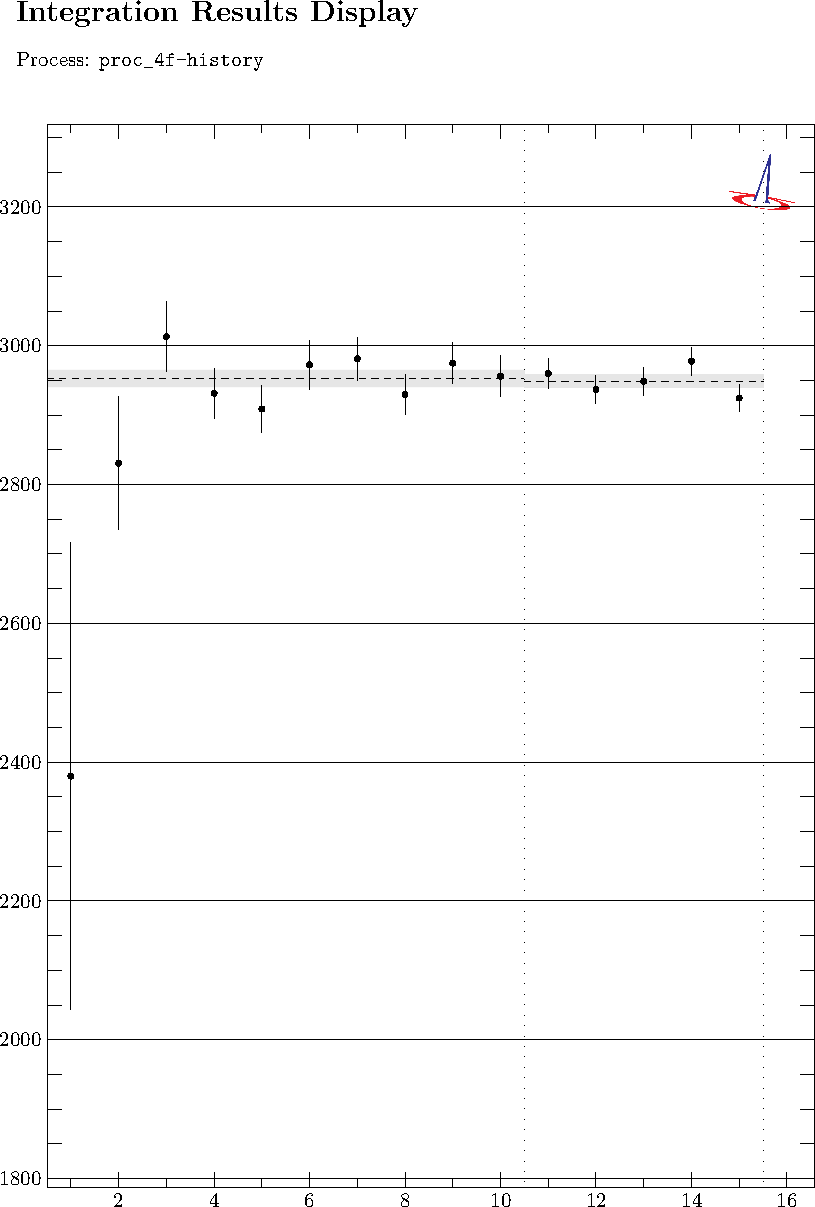
\includegraphics[width=.56\textwidth]{proc_4f-history}
  \caption{\label{fig:inthistory} Graphical output of the convergence
    of the adaptation during the integration of a \whizard\ process.}
\end{figure}
basis.  The next two columns display the error in percent, and the
\emph{accuracy} which is the same error normalized by $\sqrt{n_{\rm calls}}$.
The accuracy value has the property that it is independent of $n_{\rm calls}$,
it describes the quality of adaptation of the current grids.  Good-quality
grids have a number of order one, the smaller the better.  The next column is
the estimate for the rejection efficiency in percent.  Here, the value should
be as high as possible, with $100\,\%$ being the possible maximum.

In the example, the grids are adapted over ten iterations, after which the
accuracy and efficiency have saturated at about $1.0$ and $10\,\%$,
respectively.  The asterisk in the accuracy column marks those iterations
where an improvement over the previous iteration is seen.  The average over
these iterations exhibits an accuracy of $1.22$, corresponding to $0.39\,\%$
error, and a $\chi^2$ value of $1.15$, which is just right:
apparently, the phase-space for this process and set of cuts is
well-behaved.  The subsequent five iterations are used for obtaining
the final integral, which has an accuracy below one (error $0.3\,\%$),
while the efficiency settles at about 
$10\,\%$.  In this example, the final $\chi^2$ value happens to be quite
small, i.e., the individual results are closer together than the error
estimates would suggest.  One should nevertheless not scale down the error,
but rather scale it up if the $\chi^2$ result happens to be much larger than
unity: this often indicates sub-optimally adapted grids, which insufficiently
map some corner of phase space.

One should note that all values are subject to statistical fluctuations, since
the number of calls within each iterations is finite.  Typically, fluctuations
in the efficiency estimate are considerably larger than fluctuations in the
error/accuracy estimate.  Two subsequent runs of the same script should yield
statistically independent results which may differ in all quantities, within
the error estimates, since the seed of the random-number generator will differ
by default.

It is possible to get exactly reproducible results by setting the
random-number seed explicitly, e.g.,
\begin{quote}
\begin{footnotesize}
\begin{verbatim}
  seed = 12345  
\end{verbatim}
\end{footnotesize}
\end{quote}
at any point in the SINDARIN script.  \ttt{seed} is a predefined intrinsic
variable.  The value can be any 32bit integer.  Two runs with different seeds
can be safely taken as statistically independent. In the example
above, no seed has been set, and the seed has therefore been
determined internally by \whizard\ from the system clock.

The concluding line with the time estimate applies to a subsequent simulation
step with unweighted events, which is not actually requested in the current
example.  It is based on the timing and efficiency estimate of the most recent
iteration.

As a default, a graphical output of the integration history will be
produced (if both \LaTeX\ and \metapost\ have been available during
configuration). Fig.~\ref{fig:inthistory} shows how this looks like,
and demonstrates how a proper convergence of the integral during the
adaptation looks like. The generation of these graphical history files
can be switched off using the command \ttt{?vis\_history = false}.

%%%%%

\subsection{Integration run IDs}

A single \sindarin\ script may contain multiple calls to the
\ttt{integrate} command with different parameters.  By default,
files generated for the same process in a subsequent integration will
overwrite the previous ones.  This is undesirable when the script is
re-run: all results that have been overwritten have to be recreated.

To avoid this, the user may identify a specific run by a string-valued
ID, e.g.
\begin{quote}
\begin{footnotesize}
\begin{verbatim}
  integrate (foo) { $run_id = "first" }
\end{verbatim}
\end{footnotesize}
\end{quote}
This ID will become part of the file name for all files that are
created specifically for this run.  Often it is useful to create a run
ID from a numerical value using \ttt{sprintf}, e.g., in this scan:
\begin{quote}
\begin{footnotesize}
\begin{verbatim}
  scan real mh = (100 => 200 /+ 10) {
    $run_id = sprintf "%e" (mh)
    integrate (h_production)
  }
\end{verbatim}
\end{footnotesize}
\end{quote}

With unique run IDs, a subsequent run of the same \sindarin\ script
will be able to reuse all previous results, even if there is more than
a single integration per process.




\subsection{Controlling iterations}
\label{sec:iterations}

\whizard\ has some predefined numbers of iterations and calls for the first
and second integration pass, respectively, which depend on the number of
initial and final-state particles.  They are guesses for values that yield
good-quality grids and error values in standard situations, where no
exceptionally strong peaks or loose cuts are present in the integrand.
Actually, the large number of warmup iterations in the previous example
indicates some safety margin in that respect.

It is possible, and often advisable, to adjust the iteration and call numbers
to the particular situation.  One may reduce the default numbers to short-cut
the integration, if either less accuracy is needed, or CPU time is to be
saved.  Otherwise, if convergence is bad, the number of iterations or calls
might be increased.

To set iterations manually, there is the \ttt{iterations} command:
\begin{quote}
\begin{footnotesize}
\begin{verbatim}
  iterations = 5:50000, 3:100000  
\end{verbatim}
\end{footnotesize}
\end{quote}
This is a comma-separated list.  Each pair of values corresponds to an
integration pass.  The value before the colon is the number of iterations for
this pass, the other number is the number of calls per iteration.  

While the default number of passes is two (one for warmup, one for the final
result), you may specify a single pass
\begin{quote}
\begin{footnotesize}
\begin{verbatim}
  iterations = 5:100000  
\end{verbatim}
\end{footnotesize}
\end{quote}
where the relative channel weights will \emph{not} be adjusted (because this
is the final pass).  This is appropriate for well-behaved integrands where
weight adaptation is not necessary.

You can also define more than two passes.  That might be useful when reusing a
previous grid file with insufficient quality: specify the previous passes
as-is, so the previous results will be read in, and then a new pass for
further adaptation.

In the final pass, the default behavior is to not adapt grids and
weights anymore. Otherwise, different iterations would be correlated,
and a final reliable error estimate would not be possible. For all but
the final passes, the user can decide whether to adapt grids and
weights by attaching a string specifier to the number of iterations:
\ttt{"g"} does adapt grids, but not weights, \ttt{"w"} the other way
round. \ttt{"gw"} or \ttt{"wg"} does adapt both. By the setting
\ttt{""}, all adaptations are switched off. An example looks like
this: 
\begin{code}
  iterations = 2:10000:"gw", 3:5000
\end{code}

Since it is often not known beforehand how many iterations the grid
adaptation will need, it is generally a good idea to give the first
pass a large number of iterations.  However, in many cases these turn
out to be not necessary.  To shortcut iterations, you can set any of
\begin{quote}
\begin{footnotesize}
\begin{verbatim}
accuracy_goal
error_goal
relative_error_goal
\end{verbatim}
\end{footnotesize}
\end{quote}
to a positive value.  If this is done, \whizard\ will skip warmup
iterations once all of the specified goals are reached by the current
iteration.  The final iterations (without weight adaptation) are
always performed.


\subsection{Phase space}

Before \ttt{integrate} can start its work, it must have a phase-space
configuration for the process at hand.  The method for the phase-space
parameterization is determined by the string variable
\ttt{\$phs\_method}. At the moment there are only two options,
\ttt{"single"}, for testing purposes, that is mainly used internally,
and \whizard's traditional method, \ttt{"wood"}. This parameterization
is particularly adapted and fine-tuned for electroweak processes and
might not be the ideal for for pure jet cross sections. In future
versions of \whizard, more options for phase-space parameterizations
will be made available, e.g. the \ttt{RAMBO} algorithm and its massive
cousin, and phase-space parameterizations that take care of the
dipole-like emission structure in collinear QCD (or QED) splittings. 
For the standard method, the phase-space parameterization is laid out
in an ASCII file \ttt{\textit{<process-name>\_}i\textit{<comp>}.phs}.
Here, \ttt{{\em <process-name>}} is the process name chosen by the
user while \ttt{{\em <comp>}} is the number of the process component
of the corresponding process. This immediately shows that different
components of processes are getting different phase space setups. This
is necessary for inclusive processes, e.g. the sum of $pp \to Z + nj$
and $pp \to W + nj$, or in future versions of \whizard\ for NLO
processes, where one component is the interference between the virtual
and the Born matrix element, and another one is the subtraction terms.
Normally, you do not have to deal with this file, since \whizard\ will
generate one automatically if it does not find one. (\whizard\ is
careful to check for consistency of process definition and parameters
before using an existing file.)   

Experts might find it useful to generate a phase-space file and inspect and/or
modify it before proceeding further.  To this end, there is the parameter
\verb|?phs_only|.  If you set this \ttt{true}, \whizard\ skips the actual
integration after the phase-space file has been generated.  There is also a
parameter \verb|?vis_channels| which can be set independently; if this is
\ttt{true}, \whizard\ will generate a graphical visualization of the
phase-space parameterizations encoded in the phase-space file. This
file has to be taken with a grain of salt because phase space channels
are represented by sample Feynman diagrams for the corresponding
channel. This does however {\em not} mean that in the matrix element
other Feynman diagrams are missing (the default matrix element method,
\oMega, is not using Feynman-diagrammatic amplitudes at all).

Things might go wrong with the default phase-space generation, or manual
intervention might be necessary to improve later performance.  There are a few
parameters that control the algorithm of phase-space generation.  To
understand their meaning, you should realize that phase-space
parameterizations are modeled after (dominant) Feynman graphs for the current
process.  

\subsubsection{The main phase space setup {\em wood}}

For the main phase-space parameterization of \whizard, which is called
\ttt{"wood"}, there are many different parameters and flags that allow
to tune and customize the phase-space setup for every certain process:

The parameter \verb|phs_off_shell| controls the number of off-shell lines in
those graphs, not counting $s$-channel resonances and logarithmically enhanced
$s$- and $t$-channel lines.  The default value is $2$.  Setting it to zero
will drop everything that is not resonant or logarithmically enhanced.
Increasing it will include more subdominant graphs.  (\whizard\ increases the
value automatically if the default value does not work.)

There is a similar parameter \verb|phs_t_channel| which controls
multiperipheral graphs in the parameterizations.  The default value is $6$, so
graphs with up to $6$ $t/u$-channel lines are considered.  In particular
cases, such as $e^+e^-\to n\gamma$, all graphs are multiperipheral, and for
$n>7$ \whizard\ would find no parameterizations in the default setup.
Increasing the value of \verb|phs_t_channel| solves this problem.  (This is
presently not done automatically.)

There are two numerical parameters that describe whether particles are treated
like massless particles in particular situations.  The value of
\verb|phs_threshold_s| has the default value $50\;\GeV$.  Hence, $W$ and $Z$
are considered massive, while $b$ quarks are considered massless.  This
categorization is used for deciding whether radiation of $b$ quarks can lead
to (nearly) singular behavior, i.e., logarithmic enhancement, in the infrared
and collinear regions.  If yes, logarithmic mappings are applied to phase
space.  Analogously, \verb|phs_threshold_t| decides about potential
$t$-channel singularities.  Here, the default value is $100\;\GeV$, so
amplitudes with $W$ and $Z$ in the $t$-channel are considered as
logarithmically enhanced. For a high-energy hadron collider of 40 or
100 TeV energy, also $W$ and $Z$ in $s$-channel like situations might
be necessary to be considered massless.

Such logarithmic mappings need a dimensionful scale as parameter.  There are
three such scales, all with default value $10\;\GeV$: \verb|phs_e_scale|
(energy), \verb|phs_m_scale| (invariant mass), and \verb|phs_q_scale|
(momentum transfer).  If cuts and/or masses are such that energies, invariant
masses of particle pairs, and momentum transfer values below $10\;\GeV$ are
excluded or suppressed, the values can be kept.  In special cases they should
be changed: for instance, if you want to describe $\gamma^*\to\mu^+\mu^-$
splitting well down to the muon mass, no cuts, you may set
\verb|phs_m_scale = mmu|.  The convergence of the Monte-Carlo integration
result will be considerably faster.

There are more flags. These and more details about the phase space
parameterization will be described in Sec.~\ref{sec:wood}.


\subsection{Cuts}

\whizard~2 does not apply default cuts to the integrand.  Therefore, processes
with massless particles in the initial, intermediate, or final states may not
have a finite cross section.  This fact will manifest itself in an integration
that does not converge, or is unstable, or does not yield a reasonable error
or reweighting efficiency even for very large numbers of iterations or calls
per iterations.  When doing any calculation, you should verify first that the
result that you are going to compute is finite on physical grounds.  If not,
you have to apply cuts that make it finite.

A set of cuts is defined by the \ttt{cuts} statement.  Here is an example
\begin{quote}
\begin{footnotesize}
\begin{verbatim}
cuts = all Pt > 20 GeV [colored]  
\end{verbatim}
\end{footnotesize}
\end{quote}
This implies that events are kept only (for integration and simulation) if the
transverse momenta of all colored particles are above $20\;\GeV$.

Technically, \ttt{cuts} is a special object, which is unique within a given
scope, and is defined by the logical expression on the right-hand side of the
assignment.  It may be defined in global scope, so it is applied to all
subsequent processes.  It may be redefined by another \ttt{cuts} statement.
This overrides the first cuts setting: the \ttt{cuts} statement is not
cumulative.  Multiple cuts should be specified by the logical operators of
SINDARIN, for instance
\begin{quote}
\begin{footnotesize}
\begin{verbatim}
cuts = all Pt > 20 GeV [colored]  
  and all E > 5 GeV [photon]
\end{verbatim}
\end{footnotesize}
\end{quote}
Cuts may also be defined local to an \ttt{integrate} command, i.e., in the
options in braces.   They will apply only to the processes being integrated,
overriding any global cuts.

The right-hand side expression in the \ttt{cuts} statement is evaluated at the
point where it is used by an \ttt{integrate} command (which could be an
implicit one called by \ttt{simulate}).  Hence, if the logical expression
contains parameters, such as
\begin{quote}
\begin{footnotesize}
\begin{verbatim}
mH = 120 GeV
cuts = all M > mH [b, bbar]
mH = 150 GeV
integrate (myproc)
\end{verbatim}
\end{footnotesize}
\end{quote}
the Higgs mass value that is inserted is the value in place when
\ttt{integrate} is evaluated, $150\;\GeV$ in this example.  This same value
will also be used when the process is called by a subsequent \ttt{simulate};
it is \ttt{integrate} which compiles the cut expression and stores it among
the process data.  This behavior allows for scanning over parameters without
redefining the cuts every time.

The cut expression can make use of all variables and constructs that are
defined at the point where it is evaluated.  In particular, it can make use of
the particle content and kinematics of the hard process, as in the example
above.  In addition to the predefined variables and those defined by the user,
there are the following variables which depend on the hard process:
\begin{quote}
\begin{tabular}{ll}
integer: & \ttt{n\_in}, \ttt{n\_out}, \ttt{n\_tot} \\
real: & \ttt{sqrts}, \ttt{sqrts\_hat}
\end{tabular}
\end{quote}
Example:
\begin{quote}
\begin{footnotesize}
\begin{verbatim}
cuts = sqrts_hat > 150 GeV
\end{verbatim}
\end{footnotesize}
\end{quote}
The constants \ttt{n\_in} etc.\ are sometimes useful if a generic set of cuts
is defined, which applies to various processes simultaneously.

The user is encouraged to define his/her own set of cuts, if possible in a
process-independent manner, even if it is not required.  The \ttt{include}
command allows for storing a set of cuts in a separate SINDARIN script which
may be read in anywhere.  As an example, the system directories contain a file
\verb|default_cuts.sin| which may be invoked by
\begin{quote}
\begin{footnotesize}
\begin{verbatim}
include ("default_cuts.sin")
\end{verbatim}
\end{footnotesize}
\end{quote}


\subsection{QCD scale and coupling}

\whizard\ treats all physical parameters of a model, the coefficients in the
Lagrangian, as constants.  As a leading-order program, \whizard\ does not make
use of running parameters as they are described by renormalization theory.
For electroweak interactions where the perturbative expansion is sufficiently
well behaved, this is a consistent approach.

As far as QCD is concerned, this approach does not yield numerically
reliable results, even on the validity scale of the tree approximation.
In \whizard\ttt{2}, it is therefore possible to replace the fixed value of
$\alpha_s$ (which is accessible as the intrinsic model variable
\verb|alphas|), by a function of an energy scale $\mu$.

This is controlled by the parameter \verb|?alpha_s_is_fixed|, which is
\ttt{true} by default.  Setting it to \ttt{false} enables running~$\alpha_s$.
The user has then to decide how $\alpha_s$ is calculated.

One option is to set \verb|?alpha_s_from_lhapdf| (default \ttt{false}).  This
is recommended if the \lhapdf\ library is used for including structure
functions, but it may also be set if \lhapdf\ is not invoked.  \whizard\ will
then use the $\alpha_s$ formula and value that matches the active
\lhapdf\ structure function set and member.

In the very same way, the $\alpha_s$ running from the PDFs implemented
intrinsically in \whizard\ can be taken by setting
\verb|?alpha_s_from_pdf_builtin| to \ttt{true}. This is the same
running then the one from \lhapdf, if the intrinsic PDF coincides with
a PDF chosen from \lhapdf. 

If this is not appropriate, there are again two possibilities.  If
\verb|?alpha_s_from_mz| is \ttt{true}, the user input value \verb|alphas| is
interpreted as the running value $\alpha_s(m_Z)$, and for the particular
event, the coupling is evolved to the appropriate scale $\mu$.  The formula is
controlled by the further parameters \verb|alpha_s_order| (default $0$,
meaning leading-log; maximum $2$) and \verb|alpha_s_nf| (default $5$).

Otherwise there is the option to set \verb|?alpha_s_from_lambda_qcd = true| 
in order to evaluate $\alpha_s$ from the scale $\Lambda_{\rm QCD}$,
represented by the intrinsic variable \verb|lambda_qcd|. The reference
value for the QCD scale is $\Lambda\_{\rm QCD} = 200$
MeV. \verb|alpha_s_order| and \verb|alpha_s_nf| apply analogously. 

Note that for using one of the running options for $\alpha_s$, always 
\ttt{?alpha\_s\_is\_fixed = false} has to be invoked. 

In any case, if $\alpha_s$ is not fixed, each event has to be assigned an
energy scale.  By default, this is $\sqrt{\hat s}$, the partonic invariant
mass of the event.  This can be replaced by a user-defined scale, the special
object \ttt{scale}.  This is assigned and used just like the \ttt{cuts}
object.  The right-hand side is a real-valued expression.  Here is an example:
\begin{quote}
\begin{footnotesize}
\begin{verbatim}
scale = eval Pt [sort by -Pt [colored]]
\end{verbatim}
\end{footnotesize}
\end{quote}
This selects the $p_T$ value of the first entry in the list of colored
particles sorted by decreasing $p_T$, i.e., the $p_T$ of the hardest jet.

The \ttt{scale} definition is used not just for running $\alpha_s$ (if
enabled), but it is also the factorization scale for the \lhapdf\ structure
functions.

These two values can be set differently by specifying
\ttt{factorization\_scale} for the scale at which the PDFs are
evaluated. Analogously, there is a variable
\ttt{renormalization\_scale} that sets the scale value for the running
$\alpha_s$. Whenever any of these two values is set, it supersedes the
\ttt{scale} value. 

Just like the \ttt{cuts} expression, the expressions for \ttt{scale},
\ttt{factorization\_scale} and also \ttt{renormalization\_scale} 
are evaluated at the point where it is read by an explicit or implicit
\ttt{integrate} command.


\subsection{Reweighting factor}

It is possible to reweight the integrand by a user-defined function of the
event kinematics.  This is done by specifying a \ttt{weight} expression.
Syntax and usage is exactly analogous to the \ttt{scale} expression.  Example:
\begin{quote}
\begin{footnotesize}
\begin{verbatim}
weight = eval (1 + cos (Theta) ^ 2) [lepton]
\end{verbatim}
\end{footnotesize}
\end{quote}
We should note that the phase-space setup is not aware of this reweighting, so
in complicated cases you should not expect adaptation to achieve as accurate
results as for plain cross sections.

Needless to say, the default \ttt{weight} is unity.


\section{Events}

After the cross section integral of a scattering process is known (or the
partial-width integral of a decay process), \whizard\ can generate event
samples.  There are two limiting cases or modes of event generation:
\begin{enumerate}
\item 
  For a physics simulation, one needs \emph{unweighted} events, so the
  probability of a process and a kinematical configuration in the event sample
  is given by its squared matrix element.
\item
  Monte-Carlo integration yields \emph{weighted} events, where the probability
  (without any grid adaptation) is uniformly distributed over phase space,
  while the weight of the event is given by its squared matrix element.
\end{enumerate}
The choice of parameterizations and the iterative adaptation of the
integration grids gradually shift the generation mode from option 2 to option
1, which obviously is preferred since it simulates the actual outcome of an
experiment.  Unfortunately, this adaptation is perfect only in trivial cases,
such that the Monte-Carlo integration yields non-uniform probability still
with weighted events.  Unweighted events are obtained by rejection, i.e.,
accepting an event with a probability equal to its own weight divided by the
maximal possible weight.  Furthermore, the maximal weight is never precisely
known, so this probability can only be estimated.

The default generation mode of \whizard\ is unweighted.  This is controlled by
the parameter \verb|?unweighted| with default value \ttt{true}.  Unweighted
events are easy to interpret and can be directly compared with experiment, if
properly interfaced with detector simulation and analysis.

However, when applying rejection to generate unweighted events, the generator
discards information, and for a single event it needs, on the average,
$1/\epsilon$ calls, where the efficiency $\epsilon$ is the ratio of the
average weight over the maximal weight.  If \verb|?unweighted| is \ttt{false},
all events are kept and assigned their respective weights in histograms or
event files.


\subsection{Simulation}
\label{sec:simulation}

The \ttt{simulate} command generates an event sample.  The number of events
can be set either by specifying the integer variable \verb|n_events|, or by
the real variable \verb|luminosity|.  (This holds for unweighted events.  If
weighted events are requested, the luminosity value is ignored.)  The
luminosity is measured in 
femtobarns, but other units can be used, too.  Since the cross sections for the
processes are known at that point, the number of events is determined as the
luminosity multiplied by the cross section.

As usual, both parameters can be set either as global or as local parameters:
\begin{quote}
\begin{footnotesize}
\begin{verbatim}
  n_events = 10000
  simulate (proc1)
  simulate (proc2, proc3) { luminosity = 100 / 1 pbarn }
\end{verbatim}
\end{footnotesize}
\end{quote}
In the second example, both \verb|n_events| and \verb|luminosity| are set.  
In that case, \whizard\ chooses whatever produces the larger number of events.

If more than one process is specified in the argument of \ttt{simulate},
events are distributed among the processes with fractions proportional to
their cross section values.  The processes are mixed randomly, as it would be
the case for real data.

The raw event sample is written to a file which is named after the first process
in the argument of \ttt{simulate}.  If the process name is \ttt{proc1}, the
file will be named \ttt{proc1.evx}.  You can choose another basename by the
string variable \verb|$sample|.  For instance,
\begin{quote}
\begin{footnotesize}
\begin{verbatim}
  simulate (proc1) { n_events = 4000  $sample = "my_events" }
\end{verbatim}
\end{footnotesize}
\end{quote}
will produce an event file \verb|my_events.evx| which contains $4000$ events.

This event file is in a machine-dependent binary format, so it is not of
immediate use.  Its principal purpose is to serve as a cache: if you re-run
the same script, before starting simulation, it will look for an existing
event file that matches the input.  If nothing has changed, it will find the
file previously generated and read in the events, instead of generating them.
Thus you can modify the analysis or any further steps without repeating the
time-consuming task of generating a large event sample.  If you change the
number of events to generate, the program will make use of the existing event
sample and generate further events only when it is used up.  If necessary, you
can suppress the writing/reading of the raw event file by the parameters
\verb|?write_raw| and \verb|?read_raw|.

If you try to reuse an event file that has been written by a previous version
of \whizard, you may run into an incompatibility, which will be detected as an
error.  If this happens, you may enforce a compatibility mode (also for
writing) by setting \ttt{\$event\_file\_version} to the appropriate version
string, e.g., \verb|"2.0"|.  Be aware that this may break some more recent
features in the event analysis.

Generating an event sample can serve several purposes.  First of all,
it can be analyzed directly, by \whizard's built-in capabilities, to
produce tables, histograms, or calculate inclusive observables.  The
basic analysis features of \whizard\ are described below in
Sec.~\ref{sec:analysis}.  It can be written to an external file in a
standard format that a human or an external program can understand.
In Chap.~\ref{chap:events}, you will find a more thorough discussion
of event generation with \whizard, which also covers in detail the
available event-file formats.  Finally, \whizard\ can rescan an
existing event sample.  The event sample may either be the result of a
previous \ttt{simulate} run or, under certain conditions, an external
event sample produced by another generator or reconstructed from
data.
\begin{quote}
\begin{footnotesize}
\begin{verbatim}
rescan "my_events" (proc1) { $pdf_builtin_set = "MSTW2008LO" }
\end{verbatim}
\end{footnotesize}
\end{quote}
The rescanning may apply different parameters and recalculate the
matrix element, it may apply a different event selection, it may
reweight the events by a different PDF set (as above).  The modified
event sample can again be analyzed or written to file.  For more
details, cf.\ Sec.~\ref{sec:rescan}.

%%%%%%%%%%%%%%%

\subsection{Decays}
\label{sec:decays}

Normally, the events generated by the \ttt{simulate} command will be identical
in structure to the events that the \ttt{integrate} command generates.  This
implies that for a process such as $pp\to W^+W^-$, the final-state particles
are on-shell and stable, so they appear explicitly in the generated event
files.  If events are desired where the decay products of the $W$ bosons
appear, one has to generate another process, e.g., $pp\to u\bar d\bar ud$.  In
this case, the intermediate vector bosons, if reconstructed, are off-shell as
dictated by physics, and the process contains all intermediate states that are
possible.  In this example, the matrix element contains also $ZZ$, photon, and
non-resonant intermediate states.  (This can be restricted via the
\verb|$restrictions| option, cf.\ \ref{sec:process options}.

Another approach is to factorize the process in production (of $W$ bosons) and
decays ($W\to q\bar q$).  This is actually the traditional approach, since it
is much less computing-intensive.  The factorization neglects all off-shell
effects and irreducible background diagrams that do not have the decaying
particles as an intermediate resonance.  While \whizard\ is able to deal with
multi-particle processes without factorization, the needed computing resources
rapidly increase with the number of external particles. Particularly,
it is the phase space integration that becomes the true bottleneck for
a high multiplicity of final state particles. 

In order to use the factorized approach, one has to specify particles
as \ttt{unstable}.  (Also, the \ttt{?allow\_decays} switch must be \ttt{true};
this is however its default value.)  We give an example for a $pp \to Wj$ final
state:
\begin{code}
process wj  = u, gl => d, Wp
process wen = Wp => E1, n1

sqrts = 7 TeV
beams = p, p => pdf_builtin
unstable Wp (wen)
simulate (wj) { n_events = 1 }
\end{code}
This defines a $2 \to 2$ hard scattering process of $W + j$ production
at the 7 TeV LHC 2011 run. The $W^+$ is marked as unstable, with its
decay process being $W^+ \to e^+ \nu_e$. In the \ttt{simulate} command
both processes, the production process \ttt{wj} and the decay process
\ttt{wen} will be integrated, while the $W$ decays become effective
only in the final event sample. This event sample will contain final
states with multiplicity $3$, namely $e^+ \nu_e d$. Note that here
only one decay process is given, hence the branching ratio for the
decay will be taken to be $100 \%$ by \whizard.

A natural restriction of the factorized approach is the implied narrow-width
approximation.  Theoretically, this restriction is necessary since whenever
the width plays an important role, the usage of the factorized approach will
not be fully justified.  In particular, all involved matrix elements must be
evaluated on-shell, or otherwise gauge-invariance issues could spoil the
calculation.  (There are plans for a future \whizard\ version
to also include Breit-Wigner or Gaussian distributions when using the
factorized approach.)

Decays can be concatenated, e.g. for top pair production and
decay, $e^+ e^- \to t \bar t$ with decay $t \to W^+ b$, and subsequent
leptonic decay of the $W$ as in $W^+ \to \mu^+ \nu_\mu$:
\begin{code}
process eett = e1, E1 => t, tbar
process t_dec = t => Wp, b
process W_dec = Wp => E2, n2

unstable t (t_dec)
unstable Wp (W_dec)

sqrts = 500
simulate (eett) { n_events = 1 }
\end{code}
Note that in this case the final state in the event file will consist
of $\bar t b \mu^+ \nu_\mu$ because the anti-top is not decayed. 

If more than one decay process is being specified like in
\begin{code}
  process eeww = e1, E1 => Wp, Wm
  process w_dec1 = Wp => E2, n2
  process w_dec2 = Wp => E3, n3

  unstable Wp (w_dec1, w_dec2)
  
  sqrts = 500
  simulate (eeww) { n_events = 100 }
\end{code}
then \whizard\ takes the integrals of the specified decay processes
and distributes the decays statistically according to the calculated
branching ratio. Note that this might not be the true branching ratios
if decay processes are missing, or loop corrections to partial widths
give large(r) deviations. In the calculation of the code above,
\whizard\ will issue an output like
\begin{code}
| Unstable particle W+: computed branching ratios:
|   w_dec1: 5.0018253E-01   mu+, numu
|   w_dec2: 4.9981747E-01   tau+, nutau
|   Total width = 4.5496085E-01 GeV (computed)
|               = 2.0490000E+00 GeV (preset)
|   Decay options: helicity treated exactly  
\end{code}
So in this case, \whizard\ uses 50 \% muonic and 50 \% tauonic decays
of the positively charged $W$, while the $W^-$ appears directly in the
event file. \whizard\ shows the difference between the preset $W$
width from the physics model file and the value computed from the two
decay channels.

Note that a particle in a SINDARIN input script can be also explictly
marked as being stable, using the 
\begin{code}
stable <particle-tag>  
\end{code}
constructor for the particle \ttt{<particle-tag>}. 

\subsubsection{Spin correlations in decays}

By default, \whizard\ applies full spin and color correlations to the
factorized processes, so it keeps both color and spin coherence between
productions and decays.  Correlations between decay products of distinct
unstable particles in the same event are also fully retained.  The program
sums over all intermediate quantum numbers.

Although this approach obviously yields the optimal description with the
limits of production-decay factorization, there is support for a simplified
handling of particle decays.  Essentially, there are four options, taking a
decay \ttt{W\_ud}: $W^-\to \bar u d$ as an example:
\begin{enumerate}
\item
  Full spin correlations: \verb|unstable Wp (W_ud)|
\item
  Isotropic decay: \verb|unstable Wp (W_ud) { ?isotropic_decay = true }|
\item
  Diagonal decay matrix:
  \verb|unstable Wp (W_ud) { ?diagonal_decay = true }|
\item
  Project onto specific helicity:
  \verb|unstable Wp (W_ud) { decay_helicity = -1 }|
\end{enumerate}
Here, the isotropic option completely eliminates spin correlations.  The
diagonal-decays option eliminates just the off-diagonal entries of the $W$
spin-density matrix.  This is equivalent to a measurement of spin before the
decay.  As a result, spin correlations are still present in the classical
sense, while quantum coherence is lost.  The definite-helicity option is
similar and additional selects only the specified helicity component for the
decaying particle, so its decay distribution assumes the shape for an
accordingly polarized particle.  All options apply in the rest frame of the
decaying particle, with the particle's momentum as the quantization axis.

\subsubsection{Automatic decays}

A convenient option is if the user did not have to specify the decay
mode by hand, but if they were generated automatically. \whizard\ does
have this option: the flag \ttt{?auto\_decays} can be set to
\ttt{true}, and is taking care of that. In that case the list for the
decay processes of the particle marked as unstable is left empty (we
take a $W^-$ again as example):
\begin{code}
unstable Wm () { ?auto_decays = true }  
\end{code}
\whizard\ then inspects at the local position within the SINDARIN
input file where that \ttt{unstable} statement appears the masses of
all the particles of the active physics model in order to determine
which decays are possible. It then calculates their partial widths. 
There are a few options to customize the decays. The integer variable 
\ttt{auto\_decays\_multiplicity} allows to set the maximal
multiplicity of the final states considered in the auto decay
option. The defaul value of that variable is \ttt{2}; please be quite
careful when setting this to values larger than that. If you do so,
the flag \ttt{?auto\_decays\_radiative} allows to specify whether
final states simply containing additional resolved gluons or photons
are taken into account or not. For the example above, you almost hit
the PDG value for the $W$ total width:
\begin{code}
| Unstable particle W-: computed branching ratios:
|   decay_a24_1: 3.3337068E-01   d, ubar
|   decay_a24_2: 3.3325864E-01   s, cbar
|   decay_a24_3: 1.1112356E-01   e-, nuebar
|   decay_a24_4: 1.1112356E-01   mu-, numubar
|   decay_a24_5: 1.1112356E-01   tau-, nutaubar
|   Total width = 2.0478471E+00 GeV (computed)
|               = 2.0490000E+00 GeV (preset)
|   Decay options: helicity treated exactly  
\end{code}

\subsubsection{Future shorter notation for decays}

{\color{red} In an upcoming \whizard\ version there will be a shorter and more
  concise notation already in the process definition for such decays,
  which, however, is current not yet implemented. The two first examples
  above will then be shorter and have this form:}
  \begin{code}
    process wj = u, gl => (Wp => E1, n1), d
  \end{code}
  {\color{red} as well as }
  \begin{code}
    process eett = e1, E1 => (t => (Wp => E2, n2), b), tbar
  \end{code}

%%%%%
  
\subsection{Event formats}

As mentioned above, the internal \whizard\ event format is a
machine-dependent event format. There are a series of human-readable
ASCII event formats that are supported: very verbose formats intended
for debugging, formats that have been agreed upon during the Les
Houches workshops like LHA and LHEF, or formats that are steered
through external packages like HepMC. More details about event formats
can be found in Sec.~\ref{sec:eventformats}. 

%%%%%%%%%%%%%%%

\section{Analysis and Visualization}
\label{sec:analysis}

SINDARIN natively supports basic methods of data analysis and visualization
which are frequently used in high-energy physics studies.  Data generated
during script execution, in particular simulated event samples, can be
analyzed to evaluate further observables, fill histograms, and draw
two-dimensional plots.

So the user does not have to rely on his/her own external graphical
analysis method (like e.g. \ttt{gnuplot} or \ttt{ROOT} etc.), but can
use methods that automatically ship with \whizard. In many cases, the
user, however, clearly will use his/her own analysis machinery,
especially experimental collaborations.

In the following sections, we first summarize the available data structures,
before we consider their graphical display.



\subsection{Observables}

Analyses in high-energy physics often involve averages of quantities other
than a total cross section.  SINDARIN supports this by its \ttt{observable}
objects.  An \ttt{observable} is a container that collects a single
real-valued variable with a statistical distribution.  It is declared by a
command of the form
\begin{quote}
  \begin{footnotesize}
\ttt{observable \emph{analysis-tag}}
  \end{footnotesize}
\end{quote}
where \ttt{\emph{analysis-tag}} is an identifier that follows the same rules
as a variable name.  

Once the observable has been declared, it can be filled with values.  This is
done via the \ttt{record} command:
\begin{quote}
  \begin{footnotesize}
\ttt{record \emph{analysis-tag} (\emph{value})}
  \end{footnotesize}
\end{quote}
To make use of this, after values have been filled, we want to perform the
actual analysis and display the results.  For an observable, these are the
mean value and the standard deviation.  There is the command
\ttt{write\_analysis}:
\begin{quote}
  \begin{footnotesize}
\ttt{write\_analysis (\emph{analysis-tag})}
  \end{footnotesize}
\end{quote}

Here is an example:
\begin{quote}
  \begin{footnotesize}
\begin{verbatim}
observable obs
record obs (1.2)  record obs (1.3)  record obs (2.1)  record obs (1.4)
write_analysis (obs)
\end{verbatim}
  \end{footnotesize}
\end{quote}
The result is displayed on screen:
\begin{quote}
  \begin{footnotesize}
\begin{verbatim}
###############################################################################
# Observable: obs
average     =  1.500000000000E+00
error[abs]  =  2.041241452319E-01
error[rel]  =  1.360827634880E-01
n_entries   = 4
\end{verbatim}
  \end{footnotesize}
\end{quote}


\subsection{The analysis expression}
\label{subsec:analysis}

The most common application is the computation of event observables -- for
instance, a forward-backward asymmetry -- during simulation.  To this end,
there is an \ttt{analysis} expression, which behaves very similar to the
\ttt{cuts} expression.  It is defined either globally
\begin{quote}
  \begin{footnotesize}
    \ttt{analysis = \emph{logical-expr}}
  \end{footnotesize}
\end{quote}
or as a local option to the \ttt{simulate} or \ttt{rescan} commands which
generate and handle event samples.  If this expression is defined, it is not
evaluated immediately, but it is evaluated once for each event in the sample.

In contrast to the \ttt{cuts} expression, the logical value of the
\ttt{analysis} expression is discarded; the expression form has been chosen
just by analogy.  To make this useful, there is a variant of the \ttt{record}
command, namely a \ttt{record} function with exactly the same syntax.  As an
example, here is a calculation of the forward-backward symmetry in a process
\ttt{ee\_mumu} with final state $\mu^+\mu^-$:
\begin{quote}
  \begin{footnotesize}
\begin{verbatim}
  observable a_fb
  analysis = record a_fb (eval sgn (Pz) ["mu-"])
  simulate (ee_mumu) { luminosity = 1 / 1 fbarn }
\end{verbatim}
  \end{footnotesize}
\end{quote}
The logical return value of \ttt{record} -- which is discarded here -- is
\ttt{true} if the recording was successful.  In case of histograms (see below)
it is true if the value falls within bounds, false otherwise.

Note that the function version of \ttt{record} can be used anywhere in
expressions, not just in the \ttt{analysis} expression.

When \ttt{record} is called for an observable or histogram in simulation mode,
the recorded value is weighted appropriately.  If \ttt{?unweighted} is true,
the weight is unity, otherwise it is the event weight.

The \ttt{analysis} expression can involve any other construct
that can be expressed as an expression in SINDARIN.  For instance, this
records the energy of the 4th hardest jet in a histogram \ttt{pt\_dist}, if it
is in the central region:
\begin{quote}
  \begin{footnotesize}
\begin{verbatim}
  analysis = 
    record pt_dist (eval E [extract index 4 
                             [sort by - Pt 
                               [select if -2.5 < Eta < 2.5 [colored]]]])
\end{verbatim}
  \end{footnotesize}
\end{quote}
Here, if there is no 4th jet in the event which satisfies the criterion, the
result will be an undefined value which is not recorded.  In that case,
\ttt{record} evaluates to \ttt{false}.

Selection cuts can be part of the analysis expression:
\begin{code}
  analysis =
    if any Pt > 50 GeV [lepton] then
      record jet_energy (eval E [collect [jet]])
    endif
\end{code}
Alternatively, we can specify a separate selection expression:
\begin{code}
  selection = any Pt > 50 GeV [lepton]
  analysis = record jet_energy (eval E [collect [jet]])
\end{code}
The former version writes all events to file (if requested), but
applies the analysis expression only to the selected events.  This
allows for the simultaneous application of different selections to a
single event sample.  The latter version applies the selection to all
events before they are analyzed or written to file.

The analysis expression can make use of all variables and constructs that are
defined at the point where it is evaluated.  In particular, it can make use of
the particle content and kinematics of the hard process, as in the example
above.  In addition to the predefined variables and those defined by the user,
there are the following variables which depend on the hard process.  Some of
them are constants, some vary event by event:
\begin{quote}
\begin{tabular}{ll}
integer: &\ttt{event\_index} \\
integer: &\ttt{process\_num\_id} \\
string: &\ttt{\$process\_id} \\
integer: &\ttt{n\_in}, \ttt{n\_out}, \ttt{n\_tot} \\
real: &\ttt{sqrts}, \ttt{sqrts\_hat} \\
real: &\ttt{sqme}, \ttt{sqme\_ref} \\
real: &\ttt{event\_weight}, \ttt{event\_excess}
\end{tabular}
\end{quote}
The \ttt{process\_num\_id} is the numeric ID as used by external
programs, while the process index refers to the current library. By
default, the two are identical.  The process index itself is not
available as a predefined observable. The \ttt{sqme} and
\ttt{sqme\_ref} values indicate the squared matrix element and the
reference squared matrix element, respectively.  The latter applies
when comparing with a reference sample (the \ttt{rescan} command).

\ttt{record} evaluates to a logical, so several \ttt{record} functions may
be concatenated by the logical operators \ttt{and} or \ttt{or}.  However,
since usually the further evaluation should not depend on the return value of
\ttt{record}, it is more advisable to concatenate them by the semicolon
(\ttt{;}) operator.  This is an operator (\emph{not} a statement separator or
terminator) that connects two logical expressions and evaluates both of them
in order.  The lhs result is discarded, the result is the value of the rhs:
\begin{quote}
  \begin{footnotesize}
\begin{verbatim}
  analysis = 
    record hist_pt (eval Pt [lepton]) ; record hist_ct (eval cos (Theta) [lepton])
\end{verbatim}
  \end{footnotesize}
\end{quote}


\subsection{Histograms}
\label{sec:histogram}

In SINDARIN, a histogram is declared by the command
\begin{quote}
  \begin{footnotesize}
\ttt{histogram \emph{analysis-tag} (\emph{lower-bound}, \emph{upper-bound})}
  \end{footnotesize}
\end{quote}
This creates a histogram data structure for an (unspecified) observable.  The
entries are organized in bins between the real values \ttt{\emph{lower-bound}}
and \ttt{\emph{upper-bound}}.  The number of bins is given by the value of the
intrinsic integer variable \ttt{n\_bins}, the default value is 20.

The \ttt{histogram} declaration supports an optional argument, so the number
of bins can be set locally, for instance
\begin{quote}
  \begin{footnotesize}
\ttt{histogram pt\_distribution (0 GeV, 500 GeV) \{ n\_bins = 50 \}}
  \end{footnotesize}
\end{quote}
Sometimes it is more convenient to set the bin width directly.  This can be
done in a third argument to the \ttt{histogram} command.  
\begin{quote}
  \begin{footnotesize}
\ttt{histogram pt\_distribution (0 GeV, 500 GeV, 10 GeV)}
  \end{footnotesize}
\end{quote}
If the bin width is specified this way, it overrides the setting of
\ttt{n\_bins}. 

The \ttt{record} command or function fills histograms.  A single call
\begin{quote}
  \begin{footnotesize}
\ttt{record (\emph{real-expr})}
  \end{footnotesize}
\end{quote}
puts the value of \ttt{\emph{real-expr}} into the appropriate bin.  If
the call is issued during a simulation where \ttt{unweighted} is false, the
entry is weighted appropriately.

If the value is outside the range specified in the histogram declaration, it
is put into one of the special underflow and overflow bins.

The \ttt{write\_analysis} command prints the histogram contents as a table in
blank-separated fixed columns.  The columns are: $x$ (bin midpoint), $y$ (bin
contents), $\Delta y$ (error), excess weight, and $n$ (number of entries).
The output also contains comments initiated by a \verb|#| sign, and following
the histogram proper, information about underflow and overflow as well as
overall contents is added.


\subsection{Plots}
\label{sec:plot}

While a histogram stores only summary information about a data set, a
\ttt{plot} stores all data as $(x,y)$ pairs, optionally with errors.  A plot
declaration is as simple as
\begin{quote}
  \begin{footnotesize}
\ttt{plot \emph{analysis-tag}}
  \end{footnotesize}
\end{quote}
Like observables and histograms, plots are filled by the \ttt{record} command
or expression.  To this end, it can take two arguments,
\begin{quote}
  \begin{footnotesize}
\ttt{record (\emph{x-expr}, \emph{y-expr})}
  \end{footnotesize}
\end{quote}
or up to four:
\begin{quote}
  \begin{footnotesize}
\ttt{record (\emph{x-expr}, \emph{y-expr}, \emph{y-error})}
\\
\ttt{record (\emph{x-expr}, \emph{y-expr}, 
  \emph{y-error-expr}, \emph{x-error-expr})}
  \end{footnotesize}
\end{quote}
Note that the $y$ error comes first.  This is because applications will
demand errors for the $y$ value much more often than $x$ errors.

The plot output, again written by \ttt{write\_analysis} contains the four
values for each point, again in the ordering $x,y,\Delta y, \Delta x$.


\subsection{Analysis Output}

There is a default format for piping information into observables,
histograms, and plots. In older versions of \whizard\ there was a
first version of a custom format, which was however rather limited.
A more versatile custom output format will be coming soon. 

\begin{enumerate}
\item
By default, the \ttt{write\_analysis} command prints all data to the
standard output. The data are also written to a default file with the
name \ttt{whizard\_analysis.dat}.
Output is redirected to a file with a different name if the
variable \ttt{\$out\_file} has a nonempty value.  If the file is
already open, the output will be appended to 
the file, and it will be kept open.  If the file is not open,
\ttt{write\_analysis} will open the output file by itself, overwriting any
previous file with the same name, and close it again after data have been
written.

The command is able to print more than one dataset, following the syntax
\begin{quote}
  \begin{footnotesize}
  \ttt{write\_analysis (\emph{analysis-tag1}, \emph{analysis-tag2}, \ldots)
  \{ \emph{options} \}}
  \end{footnotesize}
\end{quote}
The argument in brackets may also be empty or absent; in this case, all
currently existing datasets are printed.

The default data format is suitable for compiling analysis data by \whizard's
built-in \gamelan\ graphics driver (see below and particularly
Chap.~\ref{chap:visualization}).  Data are written in 
blank-separated fixed columns, headlines and comments are initiated by the
\verb|#| sign, and each data set is terminated by a blank line.  However,
external programs often require special formatting.

The internal graphics driver \gamelan\ of \whizard\ is initiated by
the \ttt{compile\_analysis} command. Its syntax is the same, and it
contains the \ttt{write\_analysis} if that has not been separately
called (which is unnecessary). For more details about the \gamelan\
graphics driver and data visualization within \whizard, confer
Chap.~\ref{chap:visualization}. 

\item
Custom format. Not yet (re-)implemented in a general form.
\end{enumerate}


\section{Custom Input/Output}
\label{sec:I/O}

\whizard\ is rather chatty.  When you run examples or your own scripts, you
will observe that the program echoes most operations (assignments, commands,
etc.) on the standard output channel, i.e., on screen.  Furthermore, all
screen output is copied to a log file which by default is named
\ttt{whizard.log}.

For each integration run, \whizard\ writes additional process-specific
information to a file \ttt{\var{tag}.log}, where \ttt{\var{tag}} is the
process name.  Furthermore, the \ttt{write\_analysis} command dumps analysis
data -- tables for histograms and plots -- to its own set of files, cf.\ 
Sec.~\ref{sec:analysis}.

However, there is the occasional need to write data to extra files in a custom
format.  \sindarin\ deals with that in terms of the following commands:

\subsection{Output Files}

\subsubsection{open\_out}
\begin{syntax}
open\_out (\var{filename}) \\
open\_out (\var{filename}) \{ \var{options} \}
\end{syntax}
Open an external file for writing.  If the file exists, it is overwritten
without warning, otherwise it is created.  Example:
\begin{code}
open_out ("my_output.dat")
\end{code}


\subsubsection{close\_out}
\begin{syntax}
close\_out (\var{filename}) \\
close\_out (\var{filename}) \{ \var{options} \}
\end{syntax}
Close an external file that is open for writing.  Example:
\begin{code}
close_out ("my_output.dat")
\end{code}


\subsection{Printing Data}

\subsubsection{printf}
\begin{syntax}
printf \var{format-string-expr} \\
printf \var{format-string-expr} (\var{data-objects})
\end{syntax}
Format \ttt{\var{data-objects}} according to \ttt{\var{format-string-expr}}
and print the resulting string to standard output if the string variable
\ttt{\$out\_file} is undefined.  If \ttt{\$out\_file} is defined and the file
with this name is open for writing, print to this file instead.

Print a newline at the end if \ttt{?out\_advance} is true, otherwise don't
finish the line.

The \ttt{\var{format-string-expr}} must evaluate to a string.  Formatting
follows a subset of the rules for the \ttt{printf(3)} command in the \ttt{C}
language.  The supported rules are:
\begin{itemize}
\item All characters are printed as-is, with the exception of embedded
  conversion specifications.
\item Conversion specifications are initiated by a percent (\verb|%|) sign and
  followed by an optional prefix flag, an optional integer value, an optional
  dot followed by another integer, and a mandatory letter as the conversion
  specifier.
\item A percent sign immediately followed by another percent sign is
  interpreted as a single percent sign, not as a conversion specification.
\item The number of conversion specifiers must be equal to the number of data
  objects.  The data types must also match.
\item The first integer indicates the minimum field width, the second one the
  precision.  The field is expanded as needed.
\item The conversion specifiers \ttt{d} and \ttt{i} are equivalent, they
  indicate an integer value.
\item The conversion specifier \ttt{e} indicates a real value that should be
  printed in exponential notation.
\item The conversion specifier \ttt{f} indicates a real value that should be
  printed in decimal notation without exponent.
\item The conversion specifier \ttt{g} indicates a real value that should be
  printed either in exponential or in decimal notation, depending on its
  value.
\item The conversion specifier \ttt{s} indicates a logical or string value
  that should be printed as a string.
\item Possible prefixes are \verb|#| (alternate form, mandatory decimal point
  for reals), \verb|0| (zero padding), \verb|-| (left adjusted), \verb|+|
  (always print sign), `\verb| |' (print space before a positive number).
\end{itemize}
For more details, consult the \verb|printf(3)| manpage.  Note that other
conversions are not supported and will be rejected by \whizard.

The data arguments are numeric, logical or string variables or expressions.
Numeric expressions must be enclosed in parantheses.  Logical expressions must
be enclosed in parantheses prefixed by a question mark \verb|?|.  String
expressions must be enclosed in parantheses prefixed by a dollar sign
\verb|$|.  These forms behave as anonymous variables.

Note that for simply printing a text string, you may call \ttt{printf} with
just a format string and no data arguments.

Examples:
\begin{code}
printf "The W mass is %8f GeV" (mW)

int i = 2
int j = 3
printf "%i + %i = %i" (i, j, (i+j))

string $directory = "/usr/local/share"
string $file = "foo.dat"
printf "File path: %s/%s" ($directory, $file)
\end{code}
There is a related \ttt{sprintf} function, cf.~Sec.~\ref{sec:sprintf}.

%%%%%%%%%%%%%%%%%%%%%%%%%%%%%%%%%%%%%%%%%%%%%%%%%%%%%%%%%%%%%%%%%%%%%%

\section{WHIZARD next-to-leading order mode}
\subsection{Prerequisites}
A full NLO computation requires virtual matrix elements obtained from
loop diagrams. Since \oMega\ cannot calculate such diagrams, external
programs have to be used.  \whizard\ has a generic interface to each
matrix-element generator which is BLHA-compatible.  
Explicit implementations exist for \gosam\ and \openloops.

%%%%%

\subsubsection{Setting up \gosam}

The installation of \gosam\ is detailed on the HepForge page
\url{http://gosam/hepforge.org}. We mention here some of the steps
necessary to get it to be linked with \whizard.

{\bf Bug in \gosam\ installation scripts:} In many versions of
\gosam\ there is a bug in the installation scripts that is only
effective if \gosam\ is installed with superuser privileges. Then all
files in \texttt{\$installdir/share/golem} do not have read privileges
for normal users. These privileges must be given manually to all files
in that directory.

Prerequisites for \gosam\ to produce code for one-loop matrix elements
are the scientific algebra program \texttt{form} and the generator of
loop topologies and diagrams, \texttt{qgraf}.
These can be accessed via their respective webpages
\url{http://www.nikhef.nl/~form/} and
\url{http://cfif.ist.utl.pt/~paulo/qgraf.html}. Note also that both
\texttt{Java} and the Java runtime environment have to be installed in
order for \gosam\ to properly work. Furthermore, \texttt{libtool}
needs to be installed.

%%%%%

\subsubsection{Setting up \openloops}

The installation of \openloops\ is explained in detail on the HepForge page
\url{http://openloops.hepforge.org}. In the following the main steps for usage with \whizard\
are summarized.

\openloops\ can be checked out using the URL
\begin{code}
   \url{http://openloops.hepforge.org/svn/OpenLoops/branches/public}.
\end{code}
The program can simply be installed by running \texttt{scons}, of which a local version
is included in the \openloops directory. This produces the binary file \openloops, 
which is the main hook for all other usage of the program.

\openloops\ works by loading pre-compiled external libraries, which have to be installed for
each individual process. This requires the file \texttt{openloops.cfg}, which should contain
the following content:
\begin{code}
   [OpenLoops]
   process\_repositories=public, whizard\\
\end{code}
The libraries can then be installed via
\begin{code}
   ./openloops libinstall proc_name
\end{code}
A list of supported library names can be found on the \openloops\ web page. Note that a process library 
also includes all possible permutated processes, i.e. the process library $ppll$, for example, can 
also be used to compute the matrix elements for $e^+ e^- \rightarrow q \bar{q}$ (massless quarks only).

The \texttt{whizard} repository mentioned above contains dedicated loop routines for lepton collisions and decays.
They are not listed on the \openloops\ webpage. These libraries are:
\begin{itemize}
  \item \texttt{eett},
  \item \texttt{eehtt},
  \item \texttt{eettv},
  \item \texttt{eetttt},
  \item \texttt{eetbw},
  \item \texttt{eevjj},
  \item \texttt{eevvjj} (\texttt{v} corresponds to massive vector bosons, i.e. $W^\pm$ and $Z$, so this library also includes the process $e^+ e^- \rightarrow bW^+\bar{b}W^-$),
  \item \texttt{eehvvjj}, 
  \item \texttt{eellllbb} (Off-shell top-quark pair production with leptonic vector boson decay),
  \item \texttt{tbw} (Loops for top decay)
\end{itemize}
Finally, \openloops\ can be linked to \whizard\ during configuration by including
\begin{code}
  --enable-openloops --with-openloops=$OPENLOOPS_PATH,
\end{code}
where \texttt{\$OPENLOOPS\_PATH} is the directory the \openloops\ binary is located in. \openloops\ can then be used with the 
\sindarin option
\begin{code}
  $loop_me_method = "openloops".
\end{code}
\subsection{NLO cross sections}
NLO computation can be switched on in \sindarin\ with
\begin{code}
  process proc_nlo = in1, in2 => out1, ..., outN { nlo_calculation = "Components" },
\end{code}
where after the \texttt{nlo\_calculation} can be followed by a list of
strings specifying the desired NLO-components to be integrated,
i.e. \texttt{"Born"}, \texttt{"Real"}, \texttt{"Virtual"},
\texttt{"Pdf"}, (for hadron collisions) or \texttt{"Mismatch"} (for
the soft mismatch in resonance-aware computations) and
\texttt{"Full"}. The \texttt{"Full"}-option switches on all components
and is required if the total NLO result is desired. For example,
specifying
\begin{code}
  nlo_calculation = "Born", "Virtual"
\end{code}
will result in the computation of the Born and virtual component.

The integration can be carried out in two different modes: Combined
and separate integration. In the separate integration mode, each
component is integrated individually, allowing for a good overview of
their contributions to the total cross section. In the combined
integration mode, all components are added up during integration so
that the sum of them is evaluated. Here, only one integration pass
will be displayed. The default method is the separate integration.

The convergence of the integration can crucially be influenced by the
presence of resonances. A better convergence in this case is achieved
activating the resonance-aware FKS subtraction, 
\begin{code}
  $fks_method = "resonances".
\end{code}
This mode comes with an additional integration component, the
so-called soft mismatch. 

\subsection{Fixed-order NLO events}
Fixed-order NLO events are activated in the following way:
First, since only weighted events are possible,
\begin{code}
  ?unweighted = false
\end{code}
must be set. The fixed-order event generation is then activated using
\begin{code}
  ?nlo_fixed_order = true.
\end{code}
Moreover, event generation has to be carried out in the combined
integration mode.

\whizard then proceeds as in the usual simulation mode. I.e. it first
checks whether integration grids are already present and uses them if
they fit. Otherwise, it starts an integration.

Fixed-order NLO events are so far only supported in the
\texttt{HepMC}-format. The output can either be written to disk or put
into a FIFO to interface it to an analysis program.

For each of the \texttt{n\_events} specified in the Sindarin script,
the event output contains one event with Born kinematics and
$N_{\text{phs}}$ associated events with real kinematics, i.e. events
where one additional QCD particle is present. $N_{\text{phs}}$ the
number of distinct phase spaces. Two phase spaces are distinct if they
share the same resonance history but have different emitters. So, two
$\alpha_r$ can share the same phase space index.

The weight of the Born event is the sum $\mathcal{B} + \mathcal{V} +
\sum_{\alpha_r} \mathcal{C}_{\alpha_r}$, where $\mathcal{B}$ is the
Born matrix element, $\mathcal{V}$ is the virtual matrix element 
and $\mathcal{C}_{\alpha_r}$ are the subtraction terms in each
singular region. The weight of the real events is the sum of all the
non-subtracted $\mathcal{R}_{\alpha_r}$ which share the same phase
space. 

\subsection{Powheg matching}

%%%%%%%%%%%%%%%%%%%%%%%%%%%%%%%%%%%%%%%%%%%%%%%%%%%%%%%%%%%%%%%%%%%%%%%%

\chapter{Random number generators}
\label{chap:rng}

\section{General remarks}
\label{sec:rng}

\section{The TAO Random Number Generator}
\label{sec:tao}

%%%%%%%%%%%%%%%%%%%%%%%%%%%%%%%%%%%%%%%%%%%%%%%%%%%%%%%%%%%%%%%%%%%%%%%%

\chapter{Integration Methods}

\section{The Monte-Carlo integration routine: \ttt{VAMP}} 
\label{sec:vamp}

\vamp\ \cite{Ohl:1998jn}
is a multichannel extension of the \vegas\ \cite{Lepage:1980dq}
algorithm. For all possible singularities in the integrand, suitable
maps and integration channels are chosen which are then weighted and
superimposed to build the phase space parameterization. Both grids and
weights are modified in the adaption phase of the integration.

The multichannel integration algorithm is implemented as a
\fortranNinetyFive\ library with the task of mapping out the integrand
and finding suitable parameterizations being completely delegated to
the calling program (\whizard\ core in this case). This makes the
actual \vamp\ library completely agnostic of the model under
consideration. 

%%%%%%%%%%%%%%%%%%%%%%%%%%%%%%%%%%%%%%%%%%%%%%%%%%%%%%%%%%%%%%%%%%%%%%%%

\chapter{Phase space parameterizations}

\section{General remarks}

\section{The default method: \ttt{wood}}
\label{sec:wood}

%%%%%%%%%%%%%%%%%%%%%%%%%%%%%%%%%%%%%%%%%%%%%%%%%%%%%%%%%%%%%%%%%%%%%%%%

\chapter{Methods for Hard Interactions}
\label{chap:hardint}

\section{Internal unit matrix elements}
\label{sec:unit_me}

%%%%%

\section{Template matrix elements}
\label{sec:template_me}

%%%%%

\section{The O'Mega matrix element generator}
\label{sec:omega_me}

%%%%%

\section{Interface to GoSam}

\newpage

%%%%%%%%%%%%%%%%%%%%%%%%%%%%%%%%%%%%%%%%%%%%%%%%%%%%%%%%%%%%%%%%%%%%%%%%

\chapter{Implemented physics}
\label{chap:physics}

%%%%%

\section{The hard interaction models}

In this section, we give a brief overview over the different
incarnations of models for the description of the realm of subatomic
particles and their interactions inside \whizard. In
Sec.~\ref{sec:smandfriends}, the Standard Model (SM) itself and
straightforward extensions and modifications thereof in the gauge,
fermionic and Higgs sector are described. Then,
Sec.~\ref{sec:bsmmodels} gives a list and short description of all
genuine beyond the SM models (BSM) that are currently implemented in
\whizard\ and its matrix element generator \oMega. Additional models
beyond that can be integrated and handled via the interfaces to
external tools like \sarah\ and \FeynRules,
cf. Chap.~\ref{chap:extmodels}. 

%%%%%%%%%%%%%%%

\subsection{The Standard Model and friends}
\label{sec:smandfriends}


%%%%

\subsection{Beyond the Standard Model}
\label{sec:bsmmodels}

\begin{table}
        \begin{center}
           \begin{tabular}{|l|l|l|}
             \hline
             MODEL TYPE & with CKM matrix & trivial CKM \\
             \hline\hline
             Yukawa test model & \tt{---} & \tt{Test} \\
             \hline
             QED with $e,\mu,\tau,\gamma$ & \tt{---} &  \tt{QED} \\
             QCD with $d,u,s,c,b,t,g$ & \tt{---} &  \tt{QCD} \\
             Standard Model        & \tt{SM\_CKM} & \tt{SM} \\
             SM with anomalous gauge couplings &  \tt{SM\_ac\_CKM} &
             \tt{SM\_ac} \\
             SM with $Hgg$, $H\gamma\gamma$, $H\mu\mu$ &  \tt{---} &
             \tt{SM\_Higgs} \\
             SM with charge 4/3 top &  \tt{---} &
             \tt{SM\_top} \\
             SM with anomalous top couplings &  \tt{---} &
             \tt{SM\_top\_anom} \\
             SM with anomalous Higgs couplings &  \tt{---} &
             \tt{SM\_rx}/\tt{NoH\_rx}/\tt{SM\_ul} \\\hline
             SM extensions for $VV$ scattering & \tt{---} &
             \tt{SSC}/\tt{AltH}/\tt{SSC\_2}/\tt{SSC\_AltT} \\\hline
             SM with $Z'$ & \tt{---} & \tt{Zprime} \\
             \hline
             Two-Higgs Doublet Model & \tt{2HDM\_CKM} & \tt{2HDM} \\ \hline\hline
             MSSM &   \tt{MSSM\_CKM} & \tt{MSSM} \\
             \hline
             MSSM with gravitinos &   \tt{---} & \tt{MSSM\_Grav} \\
             \hline
             NMSSM &   \tt{NMSSM\_CKM} & \tt{NMSSM} \\
             \hline
             extended SUSY models &   \tt{---} & \tt{PSSSM} \\
             \hline\hline
             Littlest Higgs &  \tt{---} & \tt{Littlest} \\
             \hline
             Littlest Higgs with ungauged $U(1)$ &  \tt{---} &
             \tt{Littlest\_Eta} \\
             \hline
             Littlest Higgs with $T$ parity &  \tt{---} &
             \tt{Littlest\_Tpar} \\
             \hline
             Simplest Little Higgs (anomaly-free) &  \tt{---} &
             \tt{Simplest} \\
             \hline
             Simplest Little Higgs (universal) &  \tt{---} &
             \tt{Simplest\_univ} \\
             \hline\hline
             SM with graviton & \tt{---} & \tt{Xdim} \\
             \hline
             UED & \tt{---} & \tt{UED} \\
             \hline
             ``SQED'' with gravitino & \tt{---} & \tt{GravTest} \\
             \hline
             Augmentable SM template & \tt{---} & \tt{Template} \\
             \hline
           \end{tabular}
         \end{center}
	\caption{\label{tab:models} List of models available in
          \whizard. There are pure test models or models implemented 
          for theoretical investigations, a long list of SM variants
          as well as a large number of BSM models.}
\end{table}

\subsubsection{Strongly Interacting Models and Composite Models}

Higgsless models have been studied extensively before the Higgs boson
discovery at the LHC Run I in 2012 in order to detect possible
loopholes in the electroweak Higgs sector discovery potential of this
collider. The Threesite Higgsless Model is one of the simplest
incarnations of these models, and was one of the first BSM models
beyond SUSY and Little Higgs models that have been implemented in
\whizard~\cite{Speckner:2010zi}. It is also called the Minimal
Higgsless Model (MHM)~\cite{Chivukula:2006cg} is a  minimal
deconstructed Higgsless model which contains only the first resonance
in  the tower of Kaluza-Klein modes of a Higgsless extra-dimensional 
model. It is a non-renormalizable, effective theory whose
gauge group is an extension of the SM with an extra $SU(2)$ gauge
group.  The breaking of the extended electroweak gauge symmetry is
accomplished by a set of nonlinear sigma fields which represent the
effects of physics at a higher scale and make the theory
nonrenormalizable. The physical vector boson spectrum contains the
usual photon, $W^\pm$ and $Z$ bosons as well as a $W'^\pm$ and $Z'$
boson.  Additionally, a new set of heavy fermions are introduced to
accompany the new gauge group ``site'' which mix to form the physical
eigenstates.  This mixing is controlled by the small mixing parameter
$\epsilon_L$ which is adjusted to satisfy constraints from precision 
observables, such as the S parameter~\cite{Chivukula:2005xm}.  
Here, additional weak gauge boson production at the LHC was
one of the focus of the studies with \whizard~\cite{Ohl:2008ri}. 


\subsubsection{Supersymmetric Models}

\whizard/\oMega\ was the first multi-leg matrix-element/event
generator to include the full Minimal Supersymmetric Standard Model
(MSSM), and also the NMSSM. The SUSY implementations in \whizard\ have
been extensively tested~\cite{Ohl:2002jp,Reuter:2009ex}, and have been
used for many theoretical and experimental studies (some prime
examples
being~\cite{Kalinowski:2008fk,Robens:2008sa,Hagiwara:2005wg}. 

\subsubsection{Little Higgs Models}

\subsubsection{Inofficial models}

There have been several models that have been included within the
\whizard/\oMega\ framework but never found their way into the official
release series. One famous example is the non-commutative extension of
the SM, the NCSM. There have been several studies, e.g. simulations on
the $s$-channel production of a $Z$ boson at the photon collider
option of the ILC~\cite{Ohl:2004tn}. Also, the production of
electroweak gauge bosons at the LHC in the framework of the NCSM have
been studied~\cite{Ohl:2010zf}.


%%%%%%%%%%%%%%%

\section{The SUSY Les Houches Accord (SLHA) interface}
\label{sec:slha}


To be filled in
...~\cite{Skands:2003cj,AguilarSaavedra:2005pw,Allanach:2008qq}. 

The neutralino sector deserves special attention. After
diagonalization of the mass matrix expresssed in terms 
of the gaugino and higgsino eigenstates, the resulting mass
eigenvalues may be either negative or positive. In this case, two
procedures can be followed.  Either the masses are rendered
positive and the associated mixing matrix gets purely imaginary
entries or the masses are kept signed, the mixing matrix in this case
being real.  According to the SLHA agreement, the second option is
adopted. For a specific eigenvalue, the phase is absorbed into the 
definition of the relevant eigenvector, rendering the mass
negative. However, \whizard\ has not yet officially tested for
negative masses. For external SUSY models
(cf.~Chap.~\ref{chap:extmodels}) this means, that one must be careful
using a SLHA file with explicit factors of 
the complex unity in the mixing matrix, and on the other hand, 
real and positive masses for the neutralinos. For the hard-coded SUSY
models, this is completely handled internally. Especially
Ref.~\cite{Hagiwara:2005wg} discusses the details of the neutralino
(and chargino) mixing matrix.  

%%%%%%%%%%%%%%%%

\section{Lepton Collider Beam Spectra}
\label{sec:beamspectra}

For the simulation of lepton collider beam spectra there are two
dedicated tools, \circeone\ and \circetwo\ that have been written as
in principle independent tools. Both attempt to describe the
details of electron (and positron) beams in a realistic lepton
collider environment. Due to the quest for achieving high peak
luminosities at $e^+e^-$ machines, the goal is to make the spatial
extension of the beam as small as possible but keeping the area of the
beam roughly constant. This is achieved by forcing the beams in the
final focus into the shape of a quasi-2D bunch. Due to the high charge
density in that bunch, the bunch electron distribution is modified by
classical electromagnetic radiation, so called {\em beamstrahlung}. 
The two \circe\ packages are intended to perform a simulation of this
beamstrahlung and its consequences on the electron beam spectrum as
realistic as possible. More details about the two packages can be
found in their stand-alone documentations. We will discuss the basic
features of lepton-collider beam simulations in the next two sections,
including the technicalities of passing simulations of the machine
beam setup to \whizard. This will be followed by a section on the
simulation of photon collider spectra, included for historical
reasons.  

%%%%%

\subsection{\circeone}

While the bunches in a linear collider cross only once, due to their
small size they experience a strong beam-beam effect. There is a
code to simulate the impact of this effect on luminosity and
background, called
\ttt{GuineaPig++}~\cite{Schulte:1998au,Schulte:1999tx,Schulte:2007zz}.
This takes into account the details of the accelerator, the final
focus etc. on the structure of the beam and the main features of the
resulting energy spectrum of the electrons and positrons. It offers
the state-of-the-art simulation of lepton-collider beam spectra as
close as possible to reality. However, for many high-luminosity
simulations, event files produced with \texttt{GuineaPig++} are usually
too small, in the sense that not enough independent events are
available for physics simulations. Lepton collider beam spectra do
peak at the nominal beam energy ($\sqrt{s}/2$) of the collider, and
feature very steeply falling tails. Such steeply falling distributions
are very poorly mapped by histogrammed distributions with fixed bin
widths. 

The main working assumption to handle such spectra are being followed
within \circeone: 
\begin{enumerate}
\label{circe1_assumptions}
\item The beam spectra for the two beams $P_1$ and $P_2$ factorize
  (here $x_1$ and $x_2$ are the energy fractions of the two beams,
  respectively): 
  \begin{equation*}
    D_{P_1P_2} (x_1, x_2) = D_{P_1} (x_1) \cdot D_{P_2} (x_2) 
  \end{equation*}

\item
  The peak is described with a delta distribution, and the tail with a
  power law:
  \begin{equation*}
    D(x) = d \cdot \delta(1-x) \; + \; c \cdot x^\alpha \, (1-x)^\beta
  \end{equation*}
\end{enumerate}
The two powers $\alpha$ and $\beta$ are the main coefficients that can
be tuned in order to describe the spectrum with \circeone\ as close as
possible as the original \texttt{GuineaPig++} spectrum. More details
about how \circeone\ works and what it does can be found in its own
write-up in \texttt{circe1/share/doc}.

\subsection{\circetwo}

The two conditions listed in \ref{circe1_assumptions} are too
restrictive and hence insufficient to describe more complicated
lepton-collider beam spectra, as they e.g. occur in the CLIC
drive-beam design. Here, the two beams are highly correlated and also
a power-law description does not give good enough precision for the
tails. To deal with these problems, \circetwo\ starts with a
two-dimensional histogram featuring factorized, but variable bin
widths in order to simulate the steep parts of the
distributions. The limited statistics from too small
\texttt{GuineaPig++} event output files leads to correlated
fluctuations that would leave strange artifacts in the
distributions. To abandon them, Gaussian filters are applied to smooth
out the correlated fluctuations. Here care has to be taken when going
from the continuum in $x$ momentum fraction space to the corresponding
\begin{figure}
  \centering
  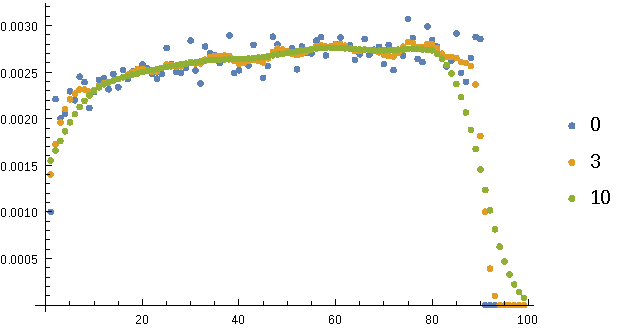
\includegraphics{circe2-smoothing}
  \caption{\label{fig:circe2smoothing}
    Smoothing the bin at the $x_{e^+} = 1$ boundary with Gaussian
    filters of 3 and 10 bins width compared to no smoothing.}
\end{figure}
boundaries: separate smoothing procedures are being applied to the
bins in the continuum region and those in the boundary in order to
avoid artificial unphysical beam energy
spreads. Fig.~\ref{fig:circe2-smoothing} shows the smoothing of the
distribution for the bin at the $x_{e^+} = 1$ boundary. The blue dots
show the direct \texttt{GuineaPig++} output comprising the
fluctuations due to the low statistics. Gaussian filters with widths
of 3 and 10 bins, respectively, have been applied (orange and green
dots, resp.). While there is still considerable fluctuation for 3 bin
width Gaussian filtering, the distribution is perfectly smooth for 10
bin width. Hence, five bin widths seem a reasonable compromise for
histograms with a total of 100 bins. Note that the bins are not
equidistant, but shrink with a power law towards the $x_{e^-} = 1$
boundary on the right hand side of Fig.~\ref{fig:circe2-smoothing}. 

\whizard\ ships (inside its subpackage \circetwo) with prepared beam
spectra ready to be used within \circetwo\ for the ILC beam spectra
used in the ILC
TDR~\cite{Behnke:2013xla,Baer:2013cma,Adolphsen:2013jya,Adolphsen:2013kya,Behnke:2013lya}. These
comprise the designed staging energies of 200 GeV, 230 GeV, 250 GeV,
350 GeV, and 500 GeV. Note that all of these spectra up to now do not
take polarization of the original beams on the beamstrahlung into
account, but are polarization-averaged. For backwards compatibility,
also the 500 GeV spectra for the TESLA
design~\cite{AguilarSaavedra:2001rg,Richard:2001qm}, here both for
polarized and polarization-averaged cases, are included. Correlated
spectra for CLIC staging energies like 350 GeV, 1400 GeV and 3000 GeV
are not yet (as of version 2.2.4) included in the \whizard\
distribution. 

In the following we describe how to obtain such files with the tools
included in \whizard (resp. \circetwo). The procedure is equivalent to
the so-called \texttt{lumi-linker} construction used by Timothy
Barklow (SLAC) together with the legacy version \whizard\texttt{ 1.95}.
The workflow to produce such files is to run \texttt{GuineaPig++} with
the following input parameters:
\begin{Code}
  do_lumi = 7;
  num_lumi = 100000000;
  num_lumi_eg = 100000000;
  num_lumi_gg = 100000000;
\end{Code}
This demands from \texttt{GuineaPig++} the generation of distributions
for the $e^-e^+$, $e^\mp \gamma$, and $\gamma\gamma$ components of the
beamstrahlung's spectrum, respectively. These are the files
\texttt{lumi.ee.out}, \texttt{lumi.eg.out}, \texttt{lumi.ge.out}, and
\texttt{lumi.gg.out}, respectively. These contain pairs $(E_1, E_2)$
of beam energies, {\em not} fractions of the original beam
energy. Huge event numbers are out in here, as \texttt{GuineaPig++}
will produce only a small fraction due to a very low generation
efficiency. 

The next step is to transfer these output files from
\texttt{GuineaPig++} into input files used with \circetwo. This is
done by means of the tool \texttt{circe\_tool.opt} that is installed
together with the \whizard\ main binary and libraries. The user should
run this executable with the following input file: 
\begin{Code}
{ file="ilc500/ilc500.circe"                   # to be loaded by WHIZARD
  { design="ILC" roots=500 bins=100 scale=250 # E in [0,1]
    { pid/1=electron pid/2=positron pol=0     # unpolarized e-/e+
      events="ilc500/lumi.ee.out" columns=2   # <= Guinea-Pig
      lumi = 1564.763360                      # <= Guinea-Pig
      iterations = 10                         # adapting bins
      smooth = 5 [0,1) [0,1)                  # Gaussian filter 5 bins
      smooth = 5 [1] [0,1) smooth = 5 [0,1) [1] } } }  
\end{Code}
The first line defines the output file, that later can be read in into
the beamstrahlung's description of \whizard\ (cf. below). Then, in the
second line the design of the collider (here: ILC for 500 GeV
center-of-mass energy, with the number of bins) is specified. The next
line tells the tool to take the unpolarized case, then the
\texttt{GuineaPig++} parameters (event file and luminosity) are
set. In the last three lines, details concerning the adaptation of the
simulation as well as the smoothing procedure are being specified: the
number of iterations in the adaptation procedure, and for the
smoothing with the Gaussian filter first in the continuum and then at
the two edges of the spectrum. For more details confer the
documentation in the \circetwo\ subpackage. 

This produces the corresponding input files that can be used within
\whizard\ to describe beamstrahlung for lepton colliders, using a
SINDARIN input file like:
\begin{Code}
        beams = e1, E1 => circe2
        $circe2_file = "ilc500.circe"
        $circe2_design = "ILC"
        ?circe2_polarized = false  
\end{Code}


%%%%%

\subsection{Photon Collider Spectra} 

For details confer the complete write-up of the \circetwo\
subpackage. 

%%%%%%%%%%%%%%%%%%%%%%%%%%%%%%%%%%%%%%%%%%%%%%%%%%%%%%%%%%%%%%%%%%%%%%%%

\chapter{More on Event Generation}
\label{chap:events}

In order to perform a physics analysis with \whizard\ one has to
generate events. This seems to be a trivial statement, but as there
have been any questions like "My \whizard\ does not produce plots --
what has gone wrong?" we believe that repeating that rule is
worthwile. Of course, it is not mandatory to use \whizard's own analysis
set-up, the user can always choose to just generate events and use
his/her own analysis package like \ttt{ROOT}, or \ttt{TopDrawer}, or
you name it for the analysis. 

Accordingly, we first start to describe how to generate events and
what options there are -- different event formats, renaming output
files, using weighted or unweighted events with different
normalizations. How to re-use and manipulate already generated event
samples, how to limit the number of events per file, etc. etc.

\section{Event generation}

To explain how event generation works, we again take our favourite
example, $e^+e^- \to \mu^+ \mu^-$,
\begin{verbatim}
  process eemm = e1, E1 => e2, E2
\end{verbatim}
The command to trigger generation of events is \ttt{simulate
  (<proc\_name>) \{ <options> \}}, so in our case -- neglecting any
options for now -- simply:
\begin{verbatim}
  simulate (eemm)
\end{verbatim}
When you run this SINDARIN file you will experience a fatal error:
\ttt{FATAL ERROR: Colliding beams: sqrts is zero (please set
sqrts)}. This is because \whizard\ needs to compile and integrate the
process \ttt{eemm} first before event simulation, because it needs the
information of the corresponding cross section, phase space
parameterization and grids. It does both automatically, but you have
to provide \whizard\ with the beam setup, or at least with the
center-of-momentum energy.  A corresponding \ttt{integrate} command
like 
\begin{verbatim}
  sqrts = 500 GeV
  integrate (eemm) { iterations = 3:10000 }
\end{verbatim}
obviously has to appear {\em before} the corresponding \ttt{simulate}
command (otherwise you would be punished by the same error message as
before). Putting things in the correct order results in an output
like:
\begin{footnotesize}
\begin{verbatim}
| Reading model file '/usr/local/share/whizard/models/SM.mdl'
| Preloaded model: SM
| Process library 'default_lib': initialized
| Preloaded library: default_lib
| Reading commands from file 'bla.sin'
| Process library 'default_lib': recorded process 'eemm'
sqrts =  5.000000000000E+02
| Integrate: current process library needs compilation
| Process library 'default_lib': compiling ...
| Process library 'default_lib': keeping makefile
| Process library 'default_lib': keeping driver
| Process library 'default_lib': active
| Process library 'default_lib': ... success.
| Integrate: compilation done
| RNG: Initializing TAO random-number generator
| RNG: Setting seed for random-number generator to 29912
| Initializing integration for process eemm:
| ------------------------------------------------------------------------
| Process [scattering]: 'eemm'
|   Library name  = 'default_lib'
|   Process index = 1
|   Process components:
|     1: 'eemm_i1':   e-, e+ => mu-, mu+ [omega]
| ------------------------------------------------------------------------
| Beam structure: [any particles]
| Beam data (collision):
|   e-  (mass = 5.1099700E-04 GeV)
|   e+  (mass = 5.1099700E-04 GeV)
|   sqrts = 5.000000000000E+02 GeV
| Phase space: generating configuration ...
| Phase space: ... success.
| Phase space: writing configuration file 'eemm_i1.phs'
| Phase space: 2 channels, 2 dimensions
| Phase space: found 2 channels, collected in 2 groves.
| Phase space: Using 2 equivalences between channels.
| Phase space: wood
Warning: No cuts have been defined.
| OpenMP: Using 8 threads
| Starting integration for process 'eemm'
| Integrate: iterations = 3:10000
| Integrator: 2 chains, 2 channels, 2 dimensions
| Integrator: Using VAMP channel equivalences
| Integrator: 10000 initial calls, 20 bins, stratified = T
| Integrator: VAMP
|=============================================================================|
| It      Calls  Integral[fb]  Error[fb]   Err[%]    Acc  Eff[%]   Chi2 N[It] |
|=============================================================================|
   1       9216  4.2833237E+02  7.14E-02    0.02    0.02*  40.29
   2       9216  4.2829071E+02  7.08E-02    0.02    0.02*  40.29
   3       9216  4.2838304E+02  7.04E-02    0.02    0.02*  40.29
|-----------------------------------------------------------------------------|
   3      27648  4.2833558E+02  4.09E-02    0.01    0.02   40.29    0.43   3
|=============================================================================|
| Time estimate for generating 10000 events: 0d:00h:00m:04s
| Creating integration history display eemm-history.ps and eemm-history.pdf
| Starting simulation for process 'eemm'
| Simulate: using integration grids from file 'eemm_m1.vg'
| RNG: Initializing TAO random-number generator
| RNG: Setting seed for random-number generator to 29913
| OpenMP: Using 8 threads
| Simulation: requested number of events = 0
|             corr. to luminosity [fb-1] =   0.0000E+00
| Events: writing to raw file 'eemm.evx'
| Events: generating 0 unweighted, unpolarized events ...
| Events: event normalization mode '1'
|         ... event sample complete.
| Events: closing raw file 'eemm.evx'
| There were no errors and    1 warning(s).
| WHIZARD run finished.
|=============================================================================|
\end{verbatim}
\end{footnotesize}

So, \whizard\ tells you that it has entered simulation mode, but besides
this, it has not done anything. The next step is that you have to
demand event generation -- there are two ways to do this: you could
either specify a certain number, say 42, of events you want to have
generated by \whizard, or you could provide a number for an integrated
luminosity of some experiment. (Note, that if you choose to take both
options, \whizard\ will take the one which gives the larger event
sample. This, of course, depends on the given process(es) -- as well
as cuts -- and its corresponding cross section(s).) The first of these
options is set with the command: \ttt{n\_events = <number>}, the
second with \ttt{luminosity = <number> <opt. unit>}.

Another important point already stated several times in the manual is
that \whizard\ follows the commands in the steering SINDARIN file in a
chronological order. Hence, a given number of events or luminosity
{\em after} a \ttt{simulate} command will be ignored -- or are
relevant only for any \ttt{simulate} command potentially following
further down in the SINDARIN file. So, in our case, try:
\begin{verbatim}
 n_events = 500
 luminosity = 10
 simulate (eemm)
\end{verbatim}
Per default, numbers for integrated luminosity are understood as
inverse femtobarn. So, for the cross section above this would
correspond to 4283 events, clearly superseding the demand for 500
events. After reducing the luminosity number from ten to one inverse
femtobarn, 500 is the larger number of events taken by \whizard\ for
event generation. Now \whizard\ tells you:
\begin{verbatim}
| Simulation: requested number of events = 500
|             corr. to luminosity [fb-1] =   1.1673E+00
| Events: reading from raw file 'eemm.evx'
| Events: reading 500 unweighted, unpolarized events ...
| Events: event normalization mode '1'
| ... event file terminates after 0 events.
| Events: appending to raw file 'eemm.evx'
| Generating remaining  500 events ...
|         ... event sample complete.
| Events: closing raw file 'eemm.evx'
\end{verbatim}
I.e., it evaluates the luminosity to which the sample of 500 events
would correspond to, which is now, of course, bigger than the $1
\fb^{-1}$ explicitly given for the luminosity. Furthermore, you can
read off that a file \ttt{whizard.evx} has been generated, containing
the demanded 500 events. (It was there before containing zero events,
because to \ttt{n\_events} or \ttt{luminosity} value had been
set. \whizard\ then tried to get the events first from file before
generating new ones). Files with the suffix \ttt{.evx} are binary
format event files, using a machine-dependent \whizard-specific
event file format. Before we list the event formats supported by
\whizard, the next two sections will tell you more about unweighted and
weighted events as well as different possibilities to normalize events
in \whizard.

As already explained for the libraries, as well as the phase space and
grid files in Chap.~\ref{chap:sindarin}, \whizard\ is trying to re-use
as much information as possible. This is of course also true for the
event files. There are special MD5 check sums testing the integrity
and compatibility of the event files. If you demand for a process for
which an event file already exists (as in the example above, though it
was empty) equally many or less events than generated before,
\whizard\ will not generate again but re-use the existing events (as
already explained, the events are stored in a \whizard-own
binary event format, i.e. in a so-called \ttt{.evx} file. If you
suppress generation of that file, as will be described in subsection
\ref{sec:eventformats} then \whizard\ has to generate events all the
time). From version v2.2.0 of \whizard\ on, the program is also able
to read in event from different event formats. However, most event
formats do not contain as many information as \whizard's internal
format, and a complete reconstruction of the events might not be
possible. Re-using event files is very practical for doing several
different analyses with the same data, especially if there are many
and big data samples. Consider 
the case, there is an event file with 200 events, and you now ask
\whizard\ to generate 300 events, then it will re-use the 200 events
(if MD5 check sums are OK!), generate the remaining 100 events and
append them to the existing file. If the user for some reason,
however, wants to regenerate events (i.e. ignoring possibly existing
events), there is the command option \ttt{whizard --rebuild-events}.

%%%%%%%%%

\section{Unweighted and weighted events}

\whizard\ is able to generate unweighted events, i.e. events that are
distributed uniformly and each contribute with the same event weight
to the whole sample. This is done by mapping out the phase space of
the process under consideration according to its different phase space
channels (which each get their own weights), and then unweighting the 
sample of weighted events. Only a sample of unweighted events could in
principle be compared to a real data sample from some experiment. The
seventh column in the \whizard\ iteration/adaptation procedure tells you
about the efficiency of the grids, i.e. how well the phase space is
mapped to a flat function. The better this is achieved, the higher the
efficiency becomes, and the closer the weights of the different phase
space channels are to uniformity. This means, for higher efficiency
less weighted events ("calls") are needed to generate a single
unweighted event. An efficiency of 10 \% means that ten weighted
events are needed to generate one single unweighted event. After the
integration is done, \whizard\ uses the duration of calls during the
adaptation to estimate a time interval needed to generate 10,000
unweighted events. The ability of the adaptive mult-channel Monte
Carlo decreases with the number of integrations, i.e. with the number
of final state particles. Adding more and more final state particles
in general also increases the complexity of phase space, especially
its singularity structure. For a $2 \to 2$ process the efficiency is
roughly of the order of several tens of per cent. As a rule of thumb,
one can say that with every additional pair of final state particle
the average efficiency one can achieve decreases by a factor of five
to ten. 

The default of \whizard\ is to generate {\em unweighted} events. One can
use the logical variable \ttt{?unweighted = false} to disable
unweighting and generate weighted events. (The command
\ttt{?unweighted = true} is a tautology, because \ttt{true} is the
default for this variable.) Note that again this command has to appear
{\em before} the corresponding \ttt{simulate} command, otherwise it will
be ignored or effective only for any \ttt{simulate} command appearing
later in the SINDARIN file.

In the unweighted procedure, \whizard\ is keeping track of the highest
weight that has been appeared during the adaptation, and the
efficiency for the unweighting has been estimated from the average
value of the sampling function compared to the maximum value. In
principle, during event generation no events should be generated whose
sampling function value exceeds the maximum function value encountered
during the grid adaptation. Sometimes, however, there are numerical
fluctuations and such events are happening. They are called {\em
excess events}. \whizard\ does keep track of these excess events
during event generation and will report about them, e.g.:
\begin{code}
Warning: Encountered events with excess weight: 9 events (  0.090 %)
| Maximum excess weight = 6.083E-01
| Average excess weight = 2.112E-04  
\end{code}
Whenever in an event generation excess events appear, this shows that
the adaptation of the sampling function has not been perfect. When the
number of excess weights is a finite number of percent, you should
inspect the phase-space setup and try to improve its settings to get a
better adaptation. 

%%%%%%%%%

\section{Choice on event normalizations}

There are basically four different choices to normalize event weights
($\braket{\ldots}$ denotes the average):
\begin{enumerate}
\item $\braket{w_i} = 1$, \qquad\qquad $\Braket{\sum_i w_i} = N$
\item $\braket{w_i} = \sigma$, \qquad\qquad $\Braket{\sum_i w_i} = N
  \times \sigma$
\item $\braket{w_i} = 1/N$, \quad\qquad $\Braket{\sum_i w_i} = 1$
\item $\braket{w_i} = \sigma/N$, \quad\qquad $\Braket{\sum_i w_i} = \sigma$
\end{enumerate}
So the four options are to have the average weight equal to unity, to
the cross section of the corresponding process, to one over the number
of events, or the cross section over the event calls. In these four
cases, the event weights sum up to the event number, the event number
times the cross section, to unity, and to the cross section,
respectively. Note that neither of these really guarantees that all
event weights individually lie in the interval $0 \leq w_i \leq 1$. 

The user can steer the normalization of events by using in SINDARIN
input files the string variable \ttt{\$sample\_normalization}. The default is
\ttt{\$sample\_normalization = "auto"}, which uses option 1 for
unweighted and 2 for weighted events, respectively. Note that this is
also what the Les Houches Event Format (LHEF) demands for both types
of events. This is \whizard's preferred mode, also for the reason, that
event normalizations are independent from the number of events. Hence,
event samples can be cut or expanded without further need to adjust
the normalization. The unit normalization (option 1) can be switched
on also for weighted events by setting the event normalization
variable equal to \ttt{"1"}. Option 2 can be demanded
by setting \ttt{\$sample\_normalization = "sigma"}. Options 3 and 4 can
be set by \ttt{"1/n"} and \ttt{"sigma/n"}, respectively. \whizard\
accepts small and capital letters for these expressions. 

In the following section we show some examples when discussing the
different event formats available in \whizard.

%%%%%%%%%

\section{Event selection}

The \ttt{selection} expression (cf.\ Sec.~\ref{subsec:analysis})
reduces the event sample during generation or rescanning, selecting
only events for which the expression evaluates to \ttt{true}.  Apart
from internal analysis, the selection also applies to writing external
files.  For instance, the following code generates a $e^+e^-\to
W^+W^-$ sample with longitudinally polarized $W$ bosons only:
\begin{footnotesize}
\begin{verbatim}
process ww = "e+", "e-" => "W-", "W+"
polarized "W+"
polarized "W-"
?polarized_events = true
sqrts = 500
selection = all Hel == 0 ["W+":"W-"]
simulate (ww) { n_events = 1000 }
\end{verbatim}
\end{footnotesize}
The number of events that end up in the sample on file is equal to the
number of events with longitudinally polarized $W$s in the generated
sample, so the file will contain less than 1000 events.


%%%%%%%%%

\section{Supported event formats}
\label{sec:eventformats}

Event formats can either be distinguished whether they are plain
text (i.e. ASCII) formats or binary formats. Besides this, one can
classify event formats according to whether they are natively
supported by \whizard\ or need some external program or library to be
linked. Table~\ref{tab:eventformats} gives a complete list of all
event formats available in \whizard. The second column shows whether
these are ASCII or binary formats, the third column contains brief
remarks about the corresponding format, while the last column tells
whether external programs or libraries are needed (which is the case
only for the HepMC formats). 

The "\ttt{.evx}'' is \whizard's native binary event format. If you
\begin{table}
  \begin{center}
    \begin{tabular}{|l||l|l|r|}\hline
      Format & Type & remark & ext. \\\hline
      ascii & ASCII & \whizard\ verbose format & no
      \\
      Athena & ASCII & variant of HEPEVT & no
      \\
      debug & ASCII & most verbose \whizard\ format & no
      \\
      evx   & binary & \whizard's home-brew & no
      \\
      HepMC & ASCII & HepMC format & yes 
      \\
      HEPEVT & ASCII & \whizard~1 style & no
      \\
      LHA  & ASCII & \whizard~1/old Les Houches style &no 
      \\
      LHEF & ASCII & Les Houches accord compliant & no
      \\
      long & ASCII & variant of HEPEVT & no 
      \\
      mokka & ASCII & variant of HEPEVT & no
      \\
      short & ASCII & variant of HEPEVT & no 
      \\
      StdHEP (HEPEVT) & binary & based on HEPEVT common block  & no
      \\
      StdHEP (HEPRUP/EUP) & binary & based on HEPRUP/EUP common block
      & no \\
      Weight stream & ASCII & just weights & yes \\ 
      \hline
    \end{tabular}    
  \end{center}
  \caption{\label{tab:eventformats}
    Event formats supported by \whizard, classified according to
    ASCII/binary formats and whether an external program or library is
    needed to generate a file of this format. For both the HEPEVT and
    the LHA format there is a more verbose variant
  }
\end{table}
demand event generation and do not specify anything further, \whizard\
will write out its events exclusively in this binary format. So in the
examples discussed in the previous chapters (where we omitted all
details about event formats), in all cases this and only this internal
binary format has been generated. The generation of this raw format
can be suppressed (e.g. if you want to have only one specific event
file type) by setting the variable \verb|?write_raw = false|. However, 
if the raw event file is not present, \whizard\ is not able to re-use
existing events (e.g. from an ASCII file) and will regenerate events
for a given process. Note that from version v2.2.0 of \whizard\ on,
the program is able to (partially) reconstruct complete events also
from other formats than its internal format (e.g. LHEF), but this is
still under construction and not yet complete.

Other event formats can be written out by setting the variable
\ttt{sample\_format = <format>}, where \ttt{<format>} can be any of
the following supported variables: 
\begin{itemize}
\item \ttt{ascii}: a quite verbose ASCII format which contains lots of
  information (an example is shown in the appendix). \newline
  Standard suffix: \ttt{.evt} 
\item \ttt{debug}: an even more verbose ASCII format intended for
  debugging which prints out also information about the internal data
  structures \newline
  Standard suffix: \ttt{.debug} 
\item \ttt{hepevt}: ASCII format that writes out a specific
  incarnation of the HEPEVT common block (\whizard~1
  back-compatibility) \newline
  Standard suffix: \ttt{.hepevt} 
\item \ttt{hepevt\_verb}: more verbose version of \ttt{hepevt} (\whizard~1
  back-compatibility) \newline
  Standard suffix: \ttt{.hepevt.verb} 
\item \ttt{short}: abbreviated variant of the previous HEPEVT (\whizard\
  1 back-compatibility)  \newline
  Standard suffix: \ttt{.short.evt} 
\item \ttt{long}: HEPEVT variant that contains a little bit more
  information than the short format but less than HEPEVT (\whizard\
  1 back-compatibility)  \newline
  Standard suffix: \ttt{.long.evt} 
\item \ttt{athena}: HEPEVT variant suitable for read-out in the ATLAS
  ATHENA software environment (\whizard\
  1 back-compatibility)  \newline
  Standard suffix: \ttt{.athena.evt} 
\item \ttt{mokka}: HEPEVT variant suitable for read-out in the MOKKA
  ILC software environment \newline
  Standard suffix: \ttt{.mokka.evt} 
\item \ttt{lha}: Implementation of the Les Houches Accord as it was in
  the old MadEvent and \whizard~1 \newline
  Standard suffix: \ttt{.lha} 
\item \ttt{lha\_verb}: more verbose version of \ttt{lha} \newline
  Standard suffix: \ttt{.lha.verb} 
\item \ttt{lhef}: Formatted Les Houches Accord implementation that
  contains the XML headers \newline
  Standard suffix: \ttt{.lhe}  
\item \ttt{hepmc}: HepMC ASCII format (only available if HepMC is
  installed and correctly linked) \newline
  Standard suffix: \ttt{.hepmc} 
\item \ttt{stdhep}: StdHEP binary format based on the HEPEVT common
  block 
  \newline 
  Standard suffix: \ttt{.hep} 
\item \ttt{stdhep\_up}: StdHEP binary format based on the HEPRUP/HEPEUP
  common blocks
  \newline
  Standard suffix: \ttt{.up.hep}
\item \ttt{stdhep\_ev4}: StdHEP binary format based on the HEPEVT/HEPEV4
  common blocks
  \newline
  Standard suffix: \ttt{.ev4.hep}  
\item \ttt{weight\_stream}: Format that prints out only the event
  weight (and maybe alternative ones) \newline
  Standard suffix: \ttt{.weight.dat}
\end{itemize}
Of course, the variable \ttt{sample\_format} can contain more than one
of the above identifiers, in which case more  than one different event
file format is generated. The list above also shows the standard
suffixes for these event formats (remember, that the native binary
format of \whizard\ does have the suffix \ttt{.evx}). (The suffix of
the different event formats can even be changed by the user by setting
the corresponding variable \ttt{\$extension\_lhef = "foo"} or 
\ttt{\$extension\_ascii\_short = "bread"}. The dot is automatically
included.) 

The name of the corresponding event sample is taken to be the string
of the name of the first process in the \ttt{simulate}
statement. Remember, that conventionally the events for all processes
in one \ttt{simulate} statement will be written into one single event
file. So \ttt{simulate (proc1, proc2)} will write events for the two
processes \ttt{proc1} and \ttt{proc2} into one single event file with
name \ttt{proc1.evx}. The name can be changed by the user with the
command \ttt{\$sample = "<name>"}. 

The commands \ttt{\$sample} and \ttt{sample\_format} are both accepted
as optional arguments of a \ttt{simulate} command, so e.g. 
\ttt{simulate (proc) \{ \$sample = "foo" sample\_format = hepmc \}}
generates an event sample in the HepMC format for the process
\ttt{proc} in the file \ttt{foo.hepmc}. 

Examples for event formats, for specifications of the
event formats correspond the different accords and publicatios: 

{\bf HEPEVT:}

The HEPEVT is an ASCII event format that does not contain an event
file header. There is a one-line header for each single event,
containing four entries. The number of particles in the event
(\ttt{ISTHEP}), which is four for a fictitious example process $hh\to
hh$, but could be larger if e.g. beam remnants are demanded to be included in the
event. The second entry and third entry are the number of outgoing
particles and beam remnants, respectively. The event weight is the
last entry. For each particle in the event there are three lines: 
the first one is the status according to the HEPEVT format,
\ttt{ISTHEP}, the second one the PDG code, \ttt{IDHEP}, then there are
the one or two possible mother particle, \ttt{JMOHEP}, the first and
last possible daughter particle, \ttt{JDAHEP}, and the polarization. 
The second line contains the three momentum components, $p_x$, $p_y$,
$p_z$, the particle energy $E$, and its mass, $m$. 
The last line contains the position of the vertex in the event
reconstruction. 

\begin{scriptsize}
  \begin{verbatim}
 4 2 0  3.0574068604E+08
 2 25 0 0 3 4 0
  0.0000000000E+00  0.0000000000E+00  4.8412291828E+02  5.0000000000E+02  1.2500000000E+02
  0.0000000000E+00  0.0000000000E+00  0.0000000000E+00  0.0000000000E+00  0.0000000000E+00
 2 25 0 0 3 4 0
  0.0000000000E+00  0.0000000000E+00 -4.8412291828E+02  5.0000000000E+02  1.2500000000E+02
  0.0000000000E+00  0.0000000000E+00  0.0000000000E+00  0.0000000000E+00  0.0000000000E+00
 1 25 1 2 0 0 0
 -1.4960220911E+02 -4.6042825611E+02  0.0000000000E+00  5.0000000000E+02  1.2500000000E+02
  0.0000000000E+00  0.0000000000E+00  0.0000000000E+00  0.0000000000E+00  0.0000000000E+00
 1 25 1 2 0 0 0
  1.4960220911E+02  4.6042825611E+02  0.0000000000E+00  5.0000000000E+02  1.2500000000E+02
  0.0000000000E+00  0.0000000000E+00  0.0000000000E+00  0.0000000000E+00  0.0000000000E+00
  \end{verbatim}
\end{scriptsize}

{\bf ASCII SHORT:}

This is basically the same as the HEPEVT standard, but very much
abbreviated. The header line for each event is identical, but the first
line per particle does only contain the PDG and the polarization,
while the vertex information line is omitted.

\begin{scriptsize}
  \begin{verbatim}
 4 2 0  3.0574068604E+08
 25 0
  0.0000000000E+00  0.0000000000E+00  4.8412291828E+02  5.0000000000E+02  1.2500000000E+02
 25 0
  0.0000000000E+00  0.0000000000E+00 -4.8412291828E+02  5.0000000000E+02  1.2500000000E+02
 25 0
 -1.4960220911E+02 -4.6042825611E+02  0.0000000000E+00  5.0000000000E+02  1.2500000000E+02
 25 0
  1.4960220911E+02  4.6042825611E+02  0.0000000000E+00  5.0000000000E+02  1.2500000000E+02
  \end{verbatim}
\end{scriptsize}

{\bf ASCII LONG:}

Identical to the ASCII short format, but after each event there is a
line containg two values: the value of the sample function to be
integrated over phase space, so basically the squared matrix element
including all normalization factors, flux factor, structure functions
etc. 

\begin{scriptsize}
  \begin{verbatim}
 4 2 0  3.0574068604E+08
 25 0
  0.0000000000E+00  0.0000000000E+00  4.8412291828E+02  5.0000000000E+02  1.2500000000E+02
 25 0
  0.0000000000E+00  0.0000000000E+00 -4.8412291828E+02  5.0000000000E+02  1.2500000000E+02
 25 0
 -1.4960220911E+02 -4.6042825611E+02  0.0000000000E+00  5.0000000000E+02  1.2500000000E+02
 25 0
  1.4960220911E+02  4.6042825611E+02  0.0000000000E+00  5.0000000000E+02  1.2500000000E+02
  1.0000000000E+00  1.0000000000E+00
  \end{verbatim}
\end{scriptsize}

{\bf ATHENA:}

Quite similar to the HEPEVT ASCII format. The header line, however,
does contain only two numbers: an event counter, and the number of
particles in the event. The first line for each particle lacks the
polarization information (irrelevant for the ATHENA environment), but
has as leading entry an ordering number counting the particles in the
event. The vertex information line has only the four relevant position
entries. 


\begin{scriptsize}
  \begin{verbatim}
 0 4
 1 2 25 0 0 3 4
  0.0000000000E+00  0.0000000000E+00  4.8412291828E+02  5.0000000000E+02  1.2500000000E+02
  0.0000000000E+00  0.0000000000E+00  0.0000000000E+00  0.0000000000E+00
 2 2 25 0 0 3 4
  0.0000000000E+00  0.0000000000E+00 -4.8412291828E+02  5.0000000000E+02  1.2500000000E+02
  0.0000000000E+00  0.0000000000E+00  0.0000000000E+00  0.0000000000E+00
 3 1 25 1 2 0 0
 -1.4960220911E+02 -4.6042825611E+02  0.0000000000E+00  5.0000000000E+02  1.2500000000E+02
  0.0000000000E+00  0.0000000000E+00  0.0000000000E+00  0.0000000000E+00
 4 1 25 1 2 0 0
  1.4960220911E+02  4.6042825611E+02  0.0000000000E+00  5.0000000000E+02  1.2500000000E+02
  0.0000000000E+00  0.0000000000E+00  0.0000000000E+00  0.0000000000E+00
  \end{verbatim}
\end{scriptsize}

{\bf MOKKA:}

Quite similar to the ASCII short format, but the event entries are the
particle status, the PDG code, the first and last daughter, the 
three spatial components of the momentum, as well as the mass.

\begin{scriptsize}
\begin{verbatim}
 4 2 0  3.0574068604E+08
 2 25 3 4  0.0000000000E+00  0.0000000000E+00  4.8412291828E+02  1.2500000000E+02
 2 25 3 4  0.0000000000E+00  0.0000000000E+00 -4.8412291828E+02  1.2500000000E+02
 1 25 0 0 -1.4960220911E+02 -4.6042825611E+02  0.0000000000E+00  1.2500000000E+02
 1 25 0 0  1.4960220911E+02  4.6042825611E+02  0.0000000000E+00  1.2500000000E+02
\end{verbatim}
\end{scriptsize}

{\bf LHA:}

This is the implementation of the Les Houches Accord, as it was used
in \whizard\ 1 and the old MadEvent. There is a first line containing 
six entries: 1. the number of particles in the event, \ttt{NUP},
2. the subprocess identification index, \ttt{IDPRUP}, 3. the event
weight, \ttt{XWGTUP}, 4. the scale of the process, \ttt{SCALUP},
5. the value or status of $\alpha_{QED}$, \ttt{AQEDUP}, 6. the value
for $\alpha_s$, \ttt{AQCDUP}. The next seven lines contain as many
entries as there are particles in the event: the first one has the PDG
codes, \ttt{IDUP}, the next two the first and second mother of the particles,
\ttt{MOTHUP}, the fourth and fifth line the two color indices,
\ttt{ICOLUP}, the next one the status of the particle, \ttt{ISTUP},
and the last line the polarization information, \ttt{ISPINUP}. 
At the end of the event there are as lines for each particles with the
counter in the event and the four-vector of the particle. For more
information on this event format confer~\cite{LesHouches}.

\begin{scriptsize}
  \begin{verbatim}
 25 25  5.0000000000E+02  5.0000000000E+02 -1 -1 -1 -1 3 1
  1.0000000000E-01  1.0000000000E-03  1.0000000000E+00 42
     4     1  3.0574068604E+08  1.000000E+03 -1.000000E+00 -1.000000E+00
    25    25    25    25
     0     0     1     1
     0     0     2     2
     0     0     0     0
     0     0     0     0
    -1    -1     1     1
     9     9     9     9
     1  5.0000000000E+02  0.0000000000E+00  0.0000000000E+00  4.8412291828E+02
     2  5.0000000000E+02  0.0000000000E+00  0.0000000000E+00 -4.8412291828E+02
     3  5.0000000000E+02 -1.4960220911E+02 -4.6042825611E+02  0.0000000000E+00
     4  5.0000000000E+02  1.4960220911E+02  4.6042825611E+02  0.0000000000E+00
  \end{verbatim}
\end{scriptsize}

{\bf LHEF:}

This is the modern version of the Les Houches accord event format
(LHEF), for the details confer the corresponding publication~\cite{LHEF}.

\begin{scriptsize}
  \begin{verbatim}
<LesHouchesEvents version="1.0">
<header>
  <generator_name>WHIZARD</generator_name>
  <generator_version>2.3.0</generator_version>
</header>
<init>
 25 25  5.0000000000E+02  5.0000000000E+02 -1 -1 -1 -1 3 1
  1.0000000000E-01  1.0000000000E-03  1.0000000000E+00 42
</init>
<event>
 4 42  3.0574068604E+08  1.0000000000E+03 -1.0000000000E+00 -1.0000000000E+00
 25 -1 0 0 0 0  0.0000000000E+00  0.0000000000E+00  4.8412291828E+02  5.0000000000E+02  1.2500000000E+02  0.0000000000E+00  9.0000000000E+00
 25 -1 0 0 0 0  0.0000000000E+00  0.0000000000E+00 -4.8412291828E+02  5.0000000000E+02  1.2500000000E+02  0.0000000000E+00  9.0000000000E+00
 25 1 1 2 0 0 -1.4960220911E+02 -4.6042825611E+02  0.0000000000E+00  5.0000000000E+02  1.2500000000E+02  0.0000000000E+00  9.0000000000E+00
 25 1 1 2 0 0  1.4960220911E+02  4.6042825611E+02  0.0000000000E+00  5.0000000000E+02  1.2500000000E+02  0.0000000000E+00  9.0000000000E+00
</event>
</LesHouchesEvents>
  \end{verbatim}
\end{scriptsize}

Note that for the LHEF format, there are different versions according
to the different stages of agreement. They can be addressed from
within the SINDARIN file by setting the string variable
\ttt{\$lhef\_version} to one of (at the moment) three values:
\ttt{"1.0"}, \ttt{"2.0"}, or \ttt{"3.0"}. The examples above
corresponds (as is indicated in the header) to the version \ttt{"1.0"}
of the LHEF format. Additional information in form of alternative
squared matrix elements or event weights in the event are the most
prominent features of the other two more advanced versions. For more
details confer the literature.

\vspace{.5cm}

Sample files for the default ASCII format as well as for the debug
event format are shown in the appendix. 

%%%%%%%%%

\section[Interfaces to Parton Showers, Matching and
Hadronization]{Interfaces to Parton Showers, Matching\\and
  Hadronization} 

This section describes the interfaces to the internal parton shower as
well as the parton shower and hadronization routines from
\pythia. Moreover, our implementation of the MLM matching making use
of the parton showers is described. Sample \sindarin\ files are
located in the \ttt{share/examples} directory.  
All input files come in two versions, one using the internal shower,
ending in \ttt{W.sin}, and one using \pythia's shower, ending in
\ttt{P.sin}. Thus we state all file names as ending with \ttt{X.sin},
where \ttt{X} has to be replaced by either \ttt{W} or \ttt{P}. 
The input files include \ttt{EENoMatchingX.sin} and
\ttt{DrellYanNoMatchingX.sin} for $e^+ e^- \to hadrons$ and $p\bar{p}
\to Z$ without matching. The corresponding \sindarin\ files with
matching enabled are \ttt{EEMatching2X.sin} to \ttt{EEMatching5X.sin}
for $e^+ e^- \to hadrons$ with a different number of partons included
in the matrix element and \ttt{DrallYanMatchingX.sin} for Drell-Yan
with one matched emission.  

\subsection{Parton Showers and Hadronization}

From version 2.1 onwards, \whizard\ contains an implementation of an
analytic parton shower as presented in \cite{Kilian:2011ka}, providing
the opportunity to perform the parton shower from whithin
\whizard. Moreover, an interface to \pythia\ is included, which can be
used to delegate the parton shower to \pythia. The same interface can
be used to hadronize events using the generated events using \pythia's
hadronization routines. Note that by \pythia's default, when
performing initial-state radiation multiple interactions are included
and when performing the hadronization hadronic decays are included. If
required, these additional steps have to be switched off using the
corresponding arguments for \pythia's \texttt{PYGIVE} routine vie the
\ttt{\$ps\_PYTHIA\_PYGIVE} string. 

Note that from version 2.2.4 on the earlier flag
\texttt{--enable-shower} flag has been abandoned, and there is only a
flag to either compile or not compile the interally attached
\pythia\texttt{6} package (\texttt{--enable-pythia6}) last release of
the \fortran\ \pythia, v6.427) as well as the interface. It can be
invoked by the following \sindarin\ keywords:\\[2ex] 
%
\centerline{\begin{tabular}{|l|l|}
\hline\ttt{?ps\_fsr\_active = true} & master switch for final-state
parton showers\\\hline 
\ttt{?ps\_isr\_active = true} & master switch for initial-state parton
showers\\\hline 
\ttt{?hadronization\_active = true} & master switch to enable
hadronization\\\hline 
\ttt{\$shower\_method = "PYTHIA6"} & switch to use \pythiasix's parton
shower instead of \\ & 
 \whizard's own shower\\\hline
\end{tabular}}\mbox{}

\vspace{4mm}

If either \ttt{?ps\_fsr\_active} or \ttt{?ps\_isr\_active} is set to \verb|true|, the 
event will be transferred to the internal shower routines or the \pythia\ data structures,
and the chosen shower steps (initial- and final-state radiation) will be
performed. If hadronization is enabled via the \ttt{?hadronization\_active} switch, \whizard\ will call \pythia's hadronization routine.
The hadron\-ization can be applied to events showered using the internal shower or showered using \pythia's shower routines, as well as unshowered events.
Any necessary transfer of event data to \pythia\ is automatically taken care of within \whizard's shower interface.
The resulting (showered and/or hadronized) event will be transferred back to \whizard,
the former final particles will be marked as intermediate. The
analysis can be applied to a showered and/or hadronized event just
like in the unshowered/unhadronized case. Any event file can be used
and will contain the showered/hadronized event. 

Settings for the internal analytic parton shower are set via the following \sindarin\ variables:\\[2ex]
\begin{description} 
\item[\texttt{ps\_mass\_cutoff}] The cut-off in virtuality, below
  which, partons are assumed to radiate no more. Used for both ISR and
  FSR. Given in $\mbox{GeV}$. (Default = 1.0)  
\item[\texttt{ps\_fsr\_lambda}] The value for $\Lambda$ used in
  calculating the value of the running coupling constant $\alpha_S$
  for Final State Radiation. Given in $\mbox{GeV}$. (Default = 0.29)  
\item[\texttt{ps\_isr\_lambda}] The value for $\Lambda$ used in
  calculating the value of the running coupling constant $\alpha_S$
  for Initial State Radiation. Given in $\mbox{GeV}$. (Default = 0.29)  
\item[\texttt{ps\_max\_n\_flavors}] Number of quark flavours taken
  into account during shower evolution. Meaningful choices are 3 to
  include $u,d,s$-quarks, 4 to include $u,d,s,c$-quarks and 5 to
  include $u,d,s,c,b$-quarks. (Default = 5)  
\item[\texttt{?ps\_isr\_alpha\_s\_running}] Switch to decide between a
  constant $\alpha_S$, given by \texttt{ps\_fixed\_alpha\_s}, and a
  running $\alpha_S$, calculated using \texttt{ps\_isr\_lambda} for
  ISR. (Default = true)  
\item[\texttt{?ps\_fsr\_alpha\_s\_running}] Switch to decide between a
  constant $\alpha_S$, given by \texttt{ps\_fixed\_alpha\_s}, and a
  running $\alpha_S$, calculated using \texttt{ps\_fsr\_lambda} for
  FSR. (Default = true)  
\item[\texttt{ps\_fixed\_alpha\_s}] Fixed value of $\alpha_S$ for the
  parton shower. Used if either one of the variables
  \texttt{?ps\_fsr\_alpha\_s\_running} 
  or \texttt{?ps\_isr\_alpha\_s\_running} are set to
  \verb|false|. (Default = 0.0)  
\item[\texttt{?ps\_isr\_angular\_ordered}] Switch for angular ordered
  ISR. (Default = true )\footnote{The FSR is always simulated with
    angular ordering enabled.} 
\item[\texttt{ps\_isr\_primordial\_kt\_width}] The width in
  $\mbox{GeV}$ of the Gaussian assumed to describe the transverse
  momentum of partons inside the proton. Other shapes are not yet
  implemented. (Default = 0.0)   
\item[\texttt{ps\_isr\_primordial\_kt\_cutoff}] The maximal transverse
  momentum in $\mbox{GeV}$ of a parton inside the proton. Used as a
  cut-off for the Gaussian. (Default = 5.0)  
\item[\texttt{ps\_isr\_z\_cutoff}] Maximal $z$-value in initial state
  branchings. (Default = 0.999)  
\item[\texttt{ps\_isr\_minenergy}] Minimal energy in $\mbox{GeV}$ of
  an emitted timelike or final parton. Note that the energy is not
  calculated in the labframe but in the center-of-mas frame of the two
  most initial partons resolved so far, so deviations may
  occur. (Default = 1.0)   
\item[\texttt{ps\_isr\_tscalefactor}] Factor for the starting scale in
  the initial state shower evolution. ( Default = 1.0 )  
\item[\texttt{?ps\_isr\_only\_onshell\_emitted\_partons}] Switch to
  allow only for on-shell emitted partons, thereby rejecting all
  possible final state parton showers starting from partons emitted
  during the ISR. (Default = false)  
\end{description}

Settings for the \pythia\ are transferred using the following
\sindarin\ variables:\\[2ex] 
\centerline{\begin{tabular}{|l|l|} 
\hline\ttt{?ps\_PYTHIA\_verbose} & if set to false, output from 
\pythia\ will be suppressed\\\hline 
\ttt{\$ps\_PYTHIA\_PYGIVE} & a string containing settings transferred
to \pythia's \ttt{PYGIVE} subroutine.\\ & The format is explained in
the \pythia\ manual. The limitation to 100 \\ & characters mentioned
there does not apply here, the string is split \\ & appropriately
before being transferred to \pythia.\\\hline 
\end{tabular}}\mbox{}

\vspace{4mm}

Note that the included version of \pythia\ uses \lhapdf\ for initial state
radiation whenever this is available, but the PDF set has to be set
manually in that case using the keyword \ttt{ps\_PYTHIA\_PYGIVE}.

\subsection{Parton shower -- Matrix Element Matching}

Along with the inclusion of the parton showers, \whizard\ includes an
implementation of the MLM matching procedure. For a detailed
description of the implemented steps see \cite{Kilian:2011ka}. The
inclusion of MLM matching still demands some manual settings in the
\sindarin\ file. For a given base process and a matching of $N$
additional jets, all processes that can be obtained by attaching up to
$N$ QCD splittings, either a quark emitting a gluon or a gluon
splitting into two quarks ar two gluons, have to be manually specified
as additional processes. These additional processes need to be
included in the \ttt{simulate} statement along with the original
process. The \sindarin\ variable \texttt{mlm\_nmaxMEjets} has to be
set to the maximum number of additional jets $N$. Moreover additional
cuts have to be specified for the additional processes.  
\begin{verbatim}
  alias quark = u:d:s:c
  alias antiq = U:D:S:C
  alias j = quark:antiq:g

  ?mlm_matching = true
  mlm_ptmin = 5 GeV
  mlm_etamax = 2.5
  mlm_Rmin = 1

  cuts = all Dist > mlm_Rmin [j, j]
         and all Pt > mlm_ptmin [j]
         and all abs(Eta) < mlm_etamax [j]
\end{verbatim}
Note that the variables \ttt{mlm\_ptmin}, \ttt{mlm\_etamax} and
\ttt{mlm\_Rmin} are used by the matching routine. Thus, replacing the
variables in the \ttt{cut} expression and omitting the assignment
would destroy the matching procedure.  

The complete list of variables introduced to steer the matching procedure is as follows:
\begin{description}
\item[\texttt{?mlm\_matching\_active}] Master switch to enable MLM
  matching. (Default = false)  
\item[\texttt{mlm\_ptmin}] Minimal transverse momentum, also used in
  the definition of a jet  
\item[\texttt{mlm\_etamax}] Maximal absolute value of pseudorapidity
  $\eta$, also used in defining a jet  
\item[\texttt{mlm\_Rmin}] Minimal $\eta-\phi$ distance $R_{min}$   
\item[\texttt{mlm\_nmaxMEjets}] Maximum number of jets $N$  
\item[\texttt{mlm\_ETclusfactor}] Factor to vary the jet
  definition. Should be $\geq 1$ for complete coverage of phase
  space. (Default = 1)  
\item[\texttt{mlm\_ETclusminE}] Minimal energy in the variation of the
  jet definition  
\item[\texttt{mlm\_etaclusfactor}] Factor in the variation of the jet
  definition. Should be $\leq 1$ for complete coverage of phase
  space. (Default = 1)  
\item[\texttt{mlm\_Rclusfactor}] Factor in the variation of the jet
  definition. Should be $\ge 1$ for complete coverage of phase
  space. (Default = 1)  
\end{description}
The variation of the jet definition is a tool to asses systematic
uncertainties introduced by the matching procedure (See section 3.1 in
\cite{Kilian:2011ka}). 
	

%%%%%%%%%

\section{Rescanning and recalculating events}
\label{sec:rescan}

In the simplest mode of execution, \whizard\ handles its events at the
point where they are generated.  It can apply event transforms such as
decays or shower (see above), it can analyze the events, calculate and
plot observables, and it can output them to file.  However, it is also
possible to apply two different operations to those events in
parallel, or to reconsider and rescan an event sample that has been
previously generated.

We first discuss the possibilities that \ttt{simulate} offers.  For
each event, \whizard\ calculates the matrix element for the hard
interaction, supplements this by Jacobian and phase-space factors in
order to obtain the event weight, optionally applies a rejection step
in order to gather uniformly weighted events, and applies the
cuts and analysis setup.  We may ask about the event matrix element or
weight, or the analysis result, that we would have obtained for a
different setting.  To this end, there is an \ttt{alt\_setup} option.

This option allows us to recalculate, event by event, the matrix
element, weight, or analysis contribution with a different parameter
set but identical kinematics.  For instance, we may evaluate a
distribution for both zero and non-zero anomalous coupling \ttt{fw}
and enter some observable in separate histograms: 

\begin{footnotesize}
\begin{verbatim}
  simulate (some_proc) {
      fw = 0
      analysis = record hist1 (eval Pt [H])
    alt_setup = {
       fw = 0.01
       analysis = record hist2 (eval Pt [H])
    }
  }
\end{verbatim}
\end{footnotesize}

In fact, the \ttt{alt\_setup} object is not restricted to a single
code block (enclosed in curly braces) but can take a list of those,
\begin{footnotesize}
\begin{verbatim}
  alt_setup = { fw = 0.01 }, { fw = 0.02 }, ...
\end{verbatim}
\end{footnotesize}
Each block provides the environment for a separate evaluation of the
event data.  The generation of these events, i.e., their kinematics,
is still steered by the primary environment.

The \ttt{alt\_setup} blocks may modify various settings that affect the
evaluation of an event, including physical parameters, PDF choice,
cuts and analysis, output format, etc.  This must not (i.e., cannot)
affect the kinematics of an event, so don't modify particle masses.
When applying cuts, they can only reduce the generated event sample,
so they apply on top of the primary cuts for the simulation.

Alternatively, it is possible to \ttt{rescan} a sample that has been
generated by a previous \ttt{simulate} command:
\begin{footnotesize}
\begin{verbatim}
  simulate (some_proc) { $sample = "my_events"
    analysis = record hist1 (eval Pt [H])
  }
  ?update_sqme = true
  ?update_weight = true
  rescan "my_events" (some_proc) {
    fw = 0.01
    analysis = record hist2 (eval Pt [H])   
  }
  rescan "my_events" (some_proc) {
    fw = 0.05
    analysis = record hist3 (eval Pt [H])   
  }
\end{verbatim}
\end{footnotesize}
In more complicated situation, rescanning is more transparent and
offers greater flexibility than doing all operations at the very point
of event generation.

Combining these features with the \ttt{scan} looping construct, we
already cover a considerable range of applications.  (There are
limitations due to the fact that \sindarin\ doesn't provide array
objects, yet.)  Note that the \ttt{rescan} construct also allows
for an \ttt{alt\_setup} option.

You may generate a new sample by rescanning, for which you may choose
any output format:
\begin{footnotesize}
\begin{verbatim}
  rescan "my_events" (some_proc) {
    selection = all Pt > 100 GeV [H]
    $sample = "new_events"
    sample_format = lhef
  }
\end{verbatim}
\end{footnotesize}

The event sample that you rescan need not be an internal raw \whizard\
file, as above.  You may rescan a LHEF file,
\begin{footnotesize}
\begin{verbatim}
  rescan "lhef_events" (proc) {
    $rescan_input_format = "lhef"
  }
\end{verbatim}
\end{footnotesize}
This file may have any origin, not necessarily from \whizard.  To
understand such an external file, \whizard\ must be able to
reconstruct the hard process and match it to a process with a known
name (e.g., \ttt{proc}), that has been defined in the \sindarin\ script
previously.

Within its limits, \whizard\ can thus be used for translating an event
sample from one format to another format.

There are three important switches that control the rescanning
behavior.  They can be set or unset independently.
\begin{itemize}
\item \ttt{?update\_sqme} (default: false).
  If true, \whizard\ will recalculate the hard matrix element for each
  event.  When applying an analysis, the recalculated squared matrix
  element (averaged and summed over quantum numbers as usual) is
  available as the variable \ttt{sqme\_prc}.  This may be related to
  \ttt{sqme\_ref}, the corresponding
  value in the event file, if available.  (For the \ttt{alt\_env}
  option, this switch is implied.)
\item \ttt{?update\_weight} (default: false).
  If true, \whizard\ will recalculate the event weight according to
  the current environment and apply this to the event.  In particular,
  the user may apply a \ttt{reweight} expression.  In an
  analysis, the new weight value is available as \ttt{weight\_prc}, to
  be related 
  to \ttt{weight\_ref} from the sample.  The updated weight will be
  applied for histograms and averages.  An unweighted event sample
  will thus be transformed into a weighted event sample.  (This switch
  is also implied for the \ttt{alt\_env} option.)
\item \ttt{?update\_event} (default: false).
  If true, \whizard\ will generate a new decay chain etc., if
  applicable.  That is, it reuses just the particles in the hard
  process.  Otherwise, the complete event is kept as it is written to
  file.
\end{itemize}
For these options to make sense, \whizard\ must have access to a full
process object, so the \sindarin\ script must contain not just a
definition but also a \ttt{compile} command for the matrix elements in
question.

If an event file (other than raw format) contains several processes as
a mixture, they must be identifiable by a numeric ID.  \whizard\ will
recognize the processes if their respective \sindarin\ definitions
contain appropriate \ttt{process\_num\_id} options, such as
\begin{footnotesize}
\begin{verbatim}
  process foo = u, ubar => d, dbar { process_num_id = 42 }
\end{verbatim}
\end{footnotesize}

Certain event-file formats, such as LHEF, support alternative
matrix-element values or weights.  \whizard\ can thus write both
original and 
recalculated matrix-element and weight values.
Other formats support only a single
event weight, so the \ttt{?update\_weight} option is necessary for a
visible effect.

External event files in formats such as LHEF, HepMC, or LCIO, also may
carry information about the value of the strong coupling $\alpha_s$
and the energy scale of each event.  This information will also be
provided by \whizard\ when writing external event files.  When such an
event file is rescanned, the user has the choice to either user the
$\alpha_s$ value that \whizard\ defines in the current context (or the
method for obtaining an event-specific running $\alpha_s$ value), or
override this for each event by using the value in the event file.
The corresponding parameter is \ttt{?use\_alpha\_s\_from\_file}, which
is false by default.  Analogously, the parameter
\ttt{?use\_scale\_from\_file} may be set to override the scale
definition in the current context.  Obviously, these settings
influence matrix-element recalculation and therefore require
\ttt{?update\_sqme} to be set in order to become operational.

%%%%%%%%%

\section{Negative weight events}
\emph{To be done.}

%%%%%%%%%%%%%%%%%%%%%%%%%%%%%%%%%%%%%%%%%%%%%%%%%%%%%%%%%%%%%%%%%%%%%%%%
\chapter{User Code Plug-Ins}
\label{chap:user}

{\color{red}
Note that the user-code plug-in mechanism has been currently (for
version 2.2.0) disabled, as the huge refactoring of the code between
versions 2.1.X and 2.2.X has completely changed many of the
interfaces. We plan to bring the interface for user code for spectra, 
structure functions and event shapes, cuts and observables back online
as soon as possible, at latest for version 2.3.0.
}

\vspace{2cm} 


\section{The plug-in mechanism}

The capabilities of \whizard\ and its \sindarin\ command
language are not always sufficient to adapt to all users' needs.  To
make the program more versatile, there are several spots in the
workflow where the user may plug in his/her own code, to enhance or
modify the default behavior.

User code can be injected, without touching \whizard's source code, in
the following places:
\begin{itemize}
\item
  Cuts, weights, analysis, etc.:
  \begin{itemize}
  \item
    Cut functions that operate on a whole subevent.
  \item
    Observable (e.g., event shapes) calculated from a whole subevent.
  \item
    Observable calculated for a particle or particle pair.
  \end{itemize}
\item
  Spectra and structure functions.
\end{itemize}
Additional plug-in locations may be added in the future.

User code is loaded dynamically by \whizard.  There are two
possibilities:
\begin{enumerate}
\item
  The user codes the required procedures in one or more Fortran source
  files that are present in the working directory of the \whizard\
  program.  \whizard\ is called with the \texttt{-u} flag:
  \begin{quote}
    \ttt{whizard -u --user-src=\emph{user-source-code-file}} \ldots
  \end{quote}
  The file must have the extension \ttt{.f90}, and the file name must
  be specified without extension.

  There may be an arbitrary number of user source-code files.  The
  compilation is done in order of appearance.  If the name of the user
  source-code file is \ttt{user.f90}, the flag \ttt{--user-src} can
  be omitted.

  This tells the program to compile and dynamically link the code at
  runtime.  The basename of the linked library is \ttt{user}.

  If a compiled (shared) library with that name already exists, it is taken
  as-is.  If the 
  user code changes or the library becomes invalid for other reasons,
  recompilation of the user-code files can be forced by the flag
  \ttt{--rebuild-user} or by the generic \ttt{-r} flag.
\item
  The user codes and compiles the required procedures him/herself.
  They should be provided in form of a library, where the interfaces of
  the individual procedures follow C calling conventions and exactly
  match the required interfaces as described in the following
  sections.  The library must be compiled in such a way that it can be
  dynamically linked.  If the calling conventions are met, the actual
  user code may be written in any programming language.  E.g., it may
  be coded in Fortran, C, or C++ (with \ttt{extern(C)} specifications).

  \whizard\ is called with the \texttt{-u} flag and is
  given the name of the user library as
  \begin{quote}
    \ttt{whizard -u --user-lib=\emph{user-library-file}} \ldots
  \end{quote}
\end{enumerate}
The library file should either be a dynamically loadable (shared)
library with appropriate extension (\ttt{.so} on Linux), or a libtool
archive (\ttt{.la}).

The user-provided procedures may have arbitrary names; the user just
has to avoid clashes with procedures from the Fortran runtime library
or from the operating-system environment.


\section{Data Types Used for Communication}
\label{sec:c_prt}

Since the user-code interface is designed to be interoperable with C,
it communicates with \whizard\ only via C-interoperable data types.
The basic data types (Fortran: integer and real kinds) \ttt{c\_int}
and \ttt{c\_double} are usually identical with the default kinds on
the Fortran side.  If necessary, explicit conversion may be inserted.

For transferring particle data, we are using a specific derived type
\ttt{c\_prt\_t} which has the following content:
\begin{quote}
\begin{footnotesize}
\begin{verbatim}
  type, bind(C) :: c_prt_t
     integer(c_int) :: type
     integer(c_int) :: pdg
     integer(c_int) :: polarized
     integer(c_int) :: h
     real(c_double) :: pe
     real(c_double) :: px
     real(c_double) :: py
     real(c_double) :: pz
     real(c_double) :: p2
  end type c_prt_t
\end{verbatim}
\end{footnotesize}
\end{quote}
The meaning of the entries is as follows:
\begin{description}
\item[\ttt{type}:] The type of the particle.  The common type
  codes are 1=incoming, 2=outgoing, and 3=composite.  A composite
  particle in a subevent is created from a combination of individual
  particle momenta, e.g., in jet clustering.  If the status code is
  not defined, it is set to zero.
\item[\ttt{pdg}:] The particle identification code as proposed by the
  Particle Data Group.  If undefined, it is zero.
\item[\ttt{polarized}:] If nonzero, the particle is polarized.  The
  only polarization scheme supported at this stage is helicity.  If
  zero, particle polarization is ignored.
\item[\ttt{h}:] If the particle is polarized, this is the helicity.  $0$
  for a scalar, $\pm 1$ for a spin-1/2 fermion, $-1,0,1$ for a spin-1
  boson.
\item[\ttt{pe}:] The energy in GeV.
\item[\ttt{px}/\ttt{py}:] The transversal momentum components in GeV.
\item[\ttt{pz}:] The longitudinal momentum component in GeV.
\item[\ttt{p2}:] The invariant mass squared of the actual momentum in GeV$^2$.
\end{description}
\whizard\ does not provide tools for manipulating \ttt{c\_prt\_t}
objects directly.  However, the four-momentum can be used in
Lorentz-algebra calculations from the \ttt{lorentz} module.  To this
end, this module defines the transformational functions
\ttt{vector4\_from\_c\_prt} and \ttt{vector4\_to\_c\_prt}.


\section{User-defined Observables and Functions}
\subsection{Cut function}
Instead of coding a cut expression in \sindarin, it may be coded in
Fortran, or in any other language with a C-compatible interface.  A
user-defined cut expression is referenced in \sindarin\ as follows:
\begin{quote}
\begin{footnotesize}
  \ttt{cuts = user\_cut (\emph{name-string}) [\emph{subevent}]}
\end{footnotesize}
\end{quote}
The \ttt{\emph{name-string}} is an expression that evaluates to
string, the name of the function to call in the user code.  The
\emph{subevent} is a subevent expression, analogous to the built-in
cut definition syntax.  The result of the \ttt{user\_cut} function is
a logical value in \sindarin.  It is true if the event passes the cut,
false otherwise.

If coded in Fortran, the actual user-cut function in the user-provided
source code has the following form:
\begin{quote}
\begin{footnotesize}
\begin{verbatim}
function user_cut_fun (prt, n_prt) result (iflag) bind(C)
   use iso_c_binding
   use c_particles
   type(c_prt_t), dimension(*), intent(in) :: prt
   integer(c_int), intent(in) :: n_prt
   integer(c_int) :: iflag
   ! ... code that evaluates iflag
end function user_cut_fun
\end{verbatim}
\end{footnotesize}
\end{quote}
Here, \ttt{user\_cut\_fun} can be replaced by an arbitrary name by
which the function is referenced as \ttt{\emph{name-string}} above.
The \ttt{bind(C)} attribute in the function declaration is mandatory.

The argument \ttt{prt} is an array of objects of type \ttt{c\_prt\_t},
as described above.  The integer \ttt{n\_prt} is the number of entries
in the array.  It is passed separately in order to determine the
actual size of the assumed-size \ttt{prt} array.

The result \ttt{iflag} is an integer.  A nonzero value indicates
\ttt{true} (i.e., the event passes the cut), zero value indicates
\ttt{false}.  (We do not use boolean values in the interface because
their interoperability might be problematic on some systems.)

\subsection{Event-shape function}

An event-shape function is similar to a cut function.  It takes a
subevent as argument and returns a real (i.e., C double) variable.  It
can be used for defining subevent observables, event weights, or the
event scale, as in
\begin{quote}
\begin{footnotesize}
  \ttt{analysis = record \emph{hist-id} (user\_event\_fun (\emph{name-string}) [\emph{subevent}])}
\end{footnotesize}
\end{quote}
or
\begin{quote}
\begin{footnotesize}
  \ttt{scale = user\_event\_fun (\emph{name-string}) [\emph{subevent}]}
\end{footnotesize}
\end{quote}
The corresponding Fortran source code has the form
\begin{quote}
\begin{footnotesize}
\begin{verbatim}
function user_event_fun (prt, n_prt) result (rval) bind(C)
   use iso_c_binding
   use c_particles
   type(c_prt_t), dimension(*), intent(in) :: prt
   integer(c_int), intent(in) :: n_prt
   real(c_double) :: rval
   ! ... code that evaluates rval
end function user_event_fun
\end{verbatim}
\end{footnotesize}
\end{quote}
with \ttt{user\_event\_fun} replaced by \ttt{\emph{name-string}}.

\subsection{Observable}

In \sindarin, an observable-type function is a function of one or two
particle objects that returns a real value.  The particle objects
result from scanning over subevents.  In the \sindarin\ code, the
observable is used like a variable; the particle-object arguments are
implictly assigned.

A user-defined observable is used analogously, e.g.,
\begin{quote}
\begin{footnotesize}
  \ttt{cuts = all user\_obs (\emph{name-string}) > 0 [\emph{subevent}]}
\end{footnotesize}
\end{quote}
The user observable is defined, as Fortran code, as either a unary or
as a binary C-double-valued function of \ttt{c\_prt\_t} objects.  The
use in \sindarin\ (unary or binary) must match the definition.
\begin{quote}
\begin{footnotesize}
\begin{verbatim}
function user_obs_unary (prt1) result (rval) bind(C)
  use iso_c_binding
  use c_particles
  type(c_prt_t), intent(in) :: prt1
  real(c_double) :: rval
  ! ... code that evaluates rval
end function user_obs_unary
\end{verbatim}
\end{footnotesize}
\end{quote}
or
\begin{quote}
\begin{footnotesize}
\begin{verbatim}
function user_obs_binary (prt1, prt2) result (rval) bind(C)
  use iso_c_binding
  use c_particles
  type(c_prt_t), intent(in) :: prt1, prt2
  real(c_double) :: rval
  ! ... code that evaluates rval
end function user_obs_binary
\end{verbatim}
\end{footnotesize}
\end{quote}
with \ttt{user\_obs\_unary}/\ttt{binary} replaced by
\ttt{\emph{name-string}}.

\subsection{Examples}

For an example, we implement three different ways of computing the
transverse momentum of a particle.  This observable is actually
built into \whizard, so the examples are not particularly useful.  However,
implementing kinematical functions that are not supported (yet) by
\whizard\ (and not easily computed via \sindarin\ expressions)
proceeds along the same lines.

\subsubsection{Cut}
The first function is a complete cut which can be used as 
\begin{quote}
  \begin{footnotesize}
    \ttt{cuts = user\_cut("ptcut") [\emph{subevt}]}
  \end{footnotesize}
\end{quote}
It is equivalent to
\begin{quote}
  \begin{footnotesize}
    \ttt{cuts = all Pt $>$ 50 [\emph{subevt}]}
  \end{footnotesize}
\end{quote}
The implementation reads
\begin{quote}
\begin{footnotesize}
\begin{verbatim}
function ptcut (prt, n_prt) result (iflag) bind(C)
  use iso_c_binding
  use c_particles
  use lorentz
  type(c_prt_t), dimension(*), intent(in) :: prt
  integer(c_int), intent(in) :: n_prt
  integer(c_int) :: iflag
  logical, save :: first = .true.
  if (all (transverse_part (vector4_from_c_prt (prt(1:n_prt))) > 50)) then
     iflag = 1
  else
     iflag = 0
  end if
end function ptcut
\end{verbatim}
\end{footnotesize}
\end{quote}
The procedure makes use of the kinematical functions in the
\ttt{lorentz} module, after transforming the particles into a
\ttt{vector4} array.

\subsubsection{Event Shape}
Similar functionality can be achieved by implementing an event-shape
function.  The function computes the minimum $p_T$ among all particles
in the subevent.  The \sindarin\ expression reads
\begin{quote}
  \begin{footnotesize}
    \ttt{cuts = user\_event\_shape("pt\_min") [\emph{subevt}] $>$ 50}
  \end{footnotesize}
\end{quote}
and the function is coded as
\begin{quote}
\begin{footnotesize}
\begin{verbatim}
function pt_min (prt, n_prt) result (rval) bind(C)
  use iso_c_binding
  use c_particles
  use lorentz
  type(c_prt_t), dimension(*), intent(in) :: prt
  integer(c_int), intent(in) :: n_prt
  real(c_double) :: rval
  rval = minval (transverse_part (vector4_from_c_prt (prt(1:n_prt))))
end function pt_min
\end{verbatim}
\end{footnotesize}
\end{quote}

\subsubsection{Observable}
The third (and probably simplest) user implementation of the $p_T$ cut
computes a single-particle observable.  Here, the usage is
\begin{quote}
  \begin{footnotesize}
    \ttt{cuts = all user\_obs("ptval") $>$ 50 [\emph{subevt}]}
  \end{footnotesize}
\end{quote}
and the subroutine reads
\begin{quote}
\begin{footnotesize}
\begin{verbatim}
function ptval (prt1) result (rval) bind(C)
  use iso_c_binding
  use c_particles
  use lorentz
  type(c_prt_t), intent(in) :: prt1
  real(c_double) :: rval
  rval = transverse_part (vector4_from_c_prt (prt1))
end function ptval
\end{verbatim}
\end{footnotesize}
\end{quote}


\section{Spectrum or Structure Function}

\subsection{Definition}

User-defined spectra or structure functions can be used in a
\ttt{beams} definition just like ordinary ones (\ttt{isr},
\ttt{pdf\_builtin}, etc.), for instance:
\begin{quote}
\begin{footnotesize}
  \ttt{beams = p, p => user\_sf (\emph{name-string})}
\end{footnotesize}
\end{quote}
or
\begin{quote}
\begin{footnotesize}
  \ttt{beams = p, "e-" => user\_sf (\emph{name-string}), none}
\end{footnotesize}
\end{quote}
To implement a particular spectrum or structure function, the user
must code five different procedures.  Their names all must begin with
\ttt{\emph{name-string}} with specific suffixes appended.  In the
following, replace \ttt{user\_sf} by whatever \ttt{\emph{name-string}}
has been chosen:
\begin{enumerate}
\item \ttt{user\_sf\_info}:\\
  This subroutine tells \whizard\ about static information on the
  spectrum.  In the user-provided source code, the function takes the
  form (if it is coded in Fortran):
  \begin{quote}
  \begin{footnotesize}
\begin{verbatim}
subroutine user_sf_info (n_in, n_out, n_states, n_col, n_dim, n_var) bind(C)
  use iso_c_binding
  integer(c_int), intent(inout) :: n_in, n_out, n_states, n_col
  integer(c_int), intent(inout) :: n_dim, n_var
  ! ... code that sets the parameters
end subroutine user_sf_info
\end{verbatim}
  \end{footnotesize}
  \end{quote}
  The subroutine arguments describe the
  overall properties of the spectrum.  For all arguments, there exist
  default values which apply if the parameter is not set in the subroutine.
  \begin{description}
  \item[\ttt{n\_in}]  Number of incoming particles.  This is 1 for a
    single-particle spectrum (default), or 2 for a two-particle
    spectrum.
  \item[\ttt{n\_out}]  Number of outgoing particles.  Should be
    greater or equal to \ttt{n\_in}.  Default is 2.
  \item[\ttt{n\_states}]  Number of distinct quantum states that are
    supported by the spectrum.  Each possible combination of flavor,
    color, and helicity counts as a separate state.  Quantum numbers
    that are ignored (e.g., unpolarized particles) do not count.
    Default is~1.
  \item[\ttt{n\_col}]  Maximal number of distinct color-flow lines
    attached to any particle.  In the Standard Model, this is 2 or less.
    Usually, the default value (2) should be left untouched.
  \item[\ttt{n\_dim}]  Number of independent integration parameters on
    which the spectrum depends.  For instance, a parton structure
    function depends on a single parameter, while ISR radiation with
    generated transverse momentum depends on three parameters.
    Default is~1.
  \item[\ttt{n\_var}]  Number of real parameters that have to be
    communicated from the kinematics routine to the evaluation
    routine.  For instance, a PDF depends on one variable ($x$) that
    is used both for computing the momentum and for evaluating the
    structure function, so it must be communicated.  Default value
    is~1.
  \end{description}
\item
  \ttt{user\_sf\_mask}:\\
  This subroutine tells \whizard\ which quantum numbers are explicit
  and which ones are ignored.  The default is that all quantum numbers
  are explicit, but it may be appropriate to ignore the polarization
  of specific particles, e.g., a radiated photon.
  \begin{quote}
  \begin{footnotesize}
\begin{verbatim}
subroutine user_sf_mask (i_prt, m_flv, m_col, m_hel, i_lock) bind(C)
  use iso_c_binding
  integer(c_int), intent(in) :: i_prt
  integer(c_int), intent(inout) :: m_flv, m_hel, m_col, i_lock
  ! ... code that sets m_flv, m_hel, m_col, i_lock
end subroutine user_sf_mask
\end{verbatim}
  \end{footnotesize}
  \end{quote}
  The arguments define the properties of a specific particle within
  the interaction that the spectrum describes.
  \begin{description}
  \item[\ttt{i\_prt}]  This is the index of the particle for which the
    info is requested.  \ttt{i\_prt}, which is a value between 1 and
    $\ttt{n\_in}+\ttt{n\_out}$.  For each possible value of
    \ttt{i\_prt}, the subroutine should set the appropriate flags,
    unless the default values are correct.  
  \item[\ttt{m\_flv}]  If nonzero, the flavor of this particle is
    unspecified.  In the process, the spectrum interaction matches any
    particle.  Default is 0.
  \item[\ttt{m\_col}]  If nonzero, the color of this particle is
    unspecified.  In the process, the spectrum interaction matches any
    color assignment, and the attached color lines are ignored for the
    whole process.  Default is 0.
  \item[\ttt{m\_hel}]  If nonzero, the helicity of this particle is
    unspecified.  In the process, the spectrum interaction matches any
    helicity assignment, i.e., the particle is treated as
    unpolarized.  Default is 0.
  \item[\ttt{i\_lock}]  If nonzero, this indicates a helicity
    conservation rule.  The current particle (\ttt{i\_prt}) and the
    particle with index \ttt{i\_lock} are declared to have the same
    helicity.

    The particle with index \ttt{i\_lock} must have a correponding
    entry pointing to index \ttt{i\_prt}.  Of course, the conservation
    rule must be satisfied by all quantum-number combination.

    (The conservation rule improves efficiency when a beam is declared as
    unpolarized.  (De-)polarization is carried through the
    structure-function chain, so that it is the hard matrix element
    which is effectively averaged over polarizations.)
  \end{description}
\item
  \ttt{user\_sf\_state}:\\
  This subroutine tells \whizard\ which quantum number combinations
  are allowed in the spectrum.  For each particles, only the quantum
  numbers allowed by the corresponding mask value (see above) have to
  be set.
  \begin{quote}
  \begin{footnotesize}
\begin{verbatim}
subroutine user_sf_state (i_state, i_prt, flv, hel, col) bind(C)
  use iso_c_binding
  integer(c_int), intent(in) :: i_state, i_prt
  integer(c_int), intent(inout) :: flv, hel
  integer(c_int), dimension(*), intent(inout) :: col
  ! ... code that sets flv, hel, col
end subroutine user_sf_state
\end{verbatim}
  \end{footnotesize}
  \end{quote}
  Given \ttt{i\_state} and \ttt{i\_prt}, the routine should return
  appropriate values for the other parameters or leave them at zero
  (default).
  \begin{description}
  \item[\ttt{i\_state}]  Index of a quantum number combination, a
    number between 1 and \ttt{n\_states}.
  \item[\ttt{i\_prt}]  Index of a particle in the interaction, a
    number between 1 and $\ttt{n\_in}+\ttt{n\_out}$.  The incoming
    particles come before the outgoing particles in the interaction.
  \item[\ttt{flv}]  PDG code of the particle.
  \item[\ttt{hel}]  Helicity value of the particle, as described above
    in Sec.~\ref{sec:c_prt}.
  \item[\ttt{col}]  Array of color-flow indices of the particle.  The
    size of the array is \ttt{n\_col}.  Color
    connections between particles are indicated by coinciding
    color-flow indices.  By convention, color-flow indices are integer
    values of $500$ and greater.
  \end{description}
\item
  \ttt{user\_sf\_kinematics}:\\
  This subroutine generates the momenta for the outgoing particles,
  given the momenta of incoming particles and an array of parameters.
  \begin{quote}
  \begin{footnotesize}
\begin{verbatim}
subroutine user_sf_kinematics (prt_in, rval, prt_out, xval) bind(C)
  use iso_c_binding
  use c_particles
  type(c_prt_t), dimension(*), intent(in) :: prt_in
  real(c_double), dimension(*), intent(in) :: rval
  type(c_prt_t), dimension(*), intent(inout) :: prt_out
  real(c_double), dimension(*), intent(out) :: xval
  ! ... code that computes prt_out and xval
end subroutine user_sf_kinematics
\end{verbatim}
  \end{footnotesize}
  \end{quote}
  \begin{description}
  \item[\ttt{prt\_in}]  Array of incoming particles as generated by
    \whizard.  Only the energy-momentum entries in the \ttt{c\_prt\_t}
    objects are relevant, the others are meaningless at this stage.
    The array size is \ttt{n\_in}.
  \item[\ttt{rval}]  Array of real parameters, sufficient for
    calculating the outgoing four-momenta.  The array size is
    \ttt{n\_dim}.
  \item[\ttt{prt\_out}]  Array of outgoing particles.  They must be
    computed by the user-defined code.  Only the energy-momentum
    entries will be used.  The array size is \ttt{n\_out}.
  \item[\ttt{xval}]  Array of parameters that are needed for the
    evaluation routine below, to uniquely determine the spectrum
    values.  For instance, these could be the $x$ momentum fraction(s)
    and possibly an extra Jacobian factor.  The array size is
    \ttt{n\_var}.
  \end{description}
\item
  \ttt{user\_sf\_evaluate}:\\
  This subroutine computes the values (the squared matrix elements) of
  the spectrum, one for each quantum-number combination, given the
  variables returned by the kinematics routine above and the energy
  scale of the event.
  \begin{quote}
  \begin{footnotesize}
\begin{verbatim}
subroutine user_sf_evaluate (xval, scale, fval) bind(C)
  use iso_c_binding
  real(c_double), dimension(*), intent(in) :: xval
  real(c_double), intent(in) :: scale
  real(c_double), dimension(*), intent(out) :: fval
end subroutine user_sf_evaluate
\end{verbatim}
  \end{footnotesize}
  \end{quote}
  \begin{description}
  \item[\ttt{xval}]  Array of parameters as returned by the kinematics
    routine.  The array size is \ttt{n\_var}.
  \item[\ttt{scale}]  Energy scale in GeV computed by \whizard\ (using
    the \sindarin\ expression for \ttt{scale}) for the current
    kinematics.  The spectrum evaluation can use this
    scale.  Alternatively, the kinematics routine may compute the scale
    and transfer it to the evaluation via the \ttt{xval} array, which
    ignores the \ttt{scale} argument.
  \item[\ttt{fval}]  Value array of the structure function.  For each
    state (combination of quantum numbers) there must be one value.
    The array size is \ttt{n\_states}.
  \end{description}
\end{enumerate}


\subsection{Example}

For a simple example, we reproduce the effect of an
\ttt{energy\_scan} spectrum for electrons, analogous to the generic
one that is built into \whizard.  We assume
that a fraction of the energy is transferred from the beam to the
incoming parton.  In contrast to the actual energy-scan spectrum where
no further particle is involved, we transfer the remaining energy to a
radiated photon.  The user-defined spectrum can be used as in
\begin{quote}
\begin{footnotesize}
  \ttt{beams = "e-", "e-" => user\_sf ("escan")}
\end{footnotesize}
\end{quote}
where it is applied to both beams, independently.

We are considering an interaction with one incoming and two outgoing
colorless particles.  There are two quantum-number states, one input
parameter, and no output parameters since the matrix element of this
spectrum is constant (unity).
\begin{quote}
  \begin{footnotesize}
\begin{verbatim}
subroutine escan_info (n_in, n_out, n_states, n_col, n_dim, n_var) bind(C)
  use iso_c_binding
  integer(c_int), intent(inout) :: n_in, n_out, n_states, n_col
  integer(c_int), intent(inout) :: n_dim, n_var
  n_in = 1
  n_out = 2
  n_states = 2
  n_dim = 1
  n_var = 0
end subroutine escan_info
\end{verbatim}
  \end{footnotesize}
\end{quote}
The mask is set up such that polarization is transferred from the
incoming to the outgoing particle (locking them together), and the
radiated photon is unpolarized.
\begin{quote}
  \begin{footnotesize}
\begin{verbatim}
subroutine escan_mask (i_prt, m_flv, m_col, m_hel, i_lock) bind(C)
  use iso_c_binding
  integer(c_int), intent(in) :: i_prt
  integer(c_int), intent(inout) :: m_flv, m_hel, m_col, i_lock
  select case (i_prt)
  case (1)
     i_lock = 3
  case (2)
     m_hel = 1
  case (3)
     i_lock = 1
  end select
end subroutine escan_mask
\end{verbatim}
  \end{footnotesize}
\end{quote}
There are two quantum-number states, one with negative and one with
positive helicity for both incoming and outgoing electron.  They are
color singlets (no color index), and the flavor of the three particles
is electron, photon, electron.
\begin{quote}
  \begin{footnotesize}
\begin{verbatim}
subroutine escan_state (i_state, i_prt, flv, hel, col) bind(C)
  use iso_c_binding
  integer(c_int), intent(in) :: i_state, i_prt
  integer(c_int), intent(inout) :: flv, hel
  integer(c_int), dimension(*), intent(inout) :: col
  select case (i_prt)
  case (1, 3)
     flv = 11
     select case (i_state)
     case (1);  hel = -1
     case (2);  hel = 1
     end select
  case (2)
     flv = 22
  end select
end subroutine escan_state
\end{verbatim}
  \end{footnotesize}
\end{quote}
The kinematics routine computes the $x$ value as $x=r^2$, where $r$ is
the integration parameter.  The four-momenta are simply scaled by the
momentum fraction, assuming zero mass.
\begin{quote}
  \begin{footnotesize}
\begin{verbatim}
subroutine escan_kinematics (prt_in, rval, prt_out, xval) bind(C)
  use iso_c_binding
  use c_particles
  use kinds
  use lorentz
  type(c_prt_t), dimension(*), intent(in) :: prt_in
  real(c_double), dimension(*), intent(in) :: rval
  type(c_prt_t), dimension(*), intent(inout) :: prt_out
  real(c_double), dimension(*), intent(out) :: xval
  type(vector4_t), dimension(3) :: p
  real(default) :: x
  x = rval(1)**2
  p(1) = vector4_from_c_prt (prt_in(1))
  p(2) = (1-x) * p(1)
  p(3) = x * p(1)
  prt_out(1:2) = vector4_to_c_prt (p(2:3))
end subroutine escan_kinematics
\end{verbatim}
  \end{footnotesize}
\end{quote}
Finally, the evaluation is trivial.  For each quantum-number state,
the matrix element is unity.
\begin{quote}
  \begin{footnotesize}
\begin{verbatim}
subroutine escan_evaluate (xval, scale, fval) bind(C)
  use iso_c_binding
  real(c_double), dimension(*), intent(in) :: xval
  real(c_double), intent(in) :: scale
  real(c_double), dimension(*), intent(out) :: fval
  fval(1) = 1
  fval(2) = 1
end subroutine escan_evaluate
\end{verbatim}
  \end{footnotesize}
\end{quote}

\section{User Code and Static Executables}

In Sec.~\ref{sec:static} we describe how to build a static executable that can
be submitted to batch jobs, e.g., on the grid, where a compiler may not be
available.

If there is user plug-in code, it would require the same setup of
libtool, compiler and linker on the target host, as physical process
code.  To avoid this, it is preferable to link the user code
statically with the executable, which is then run as a monolithic
program.

This is actually simple.  Two conditions have to be met:
\begin{enumerate}
\item
  The \whizard\ job that creates the executable has to be given the appropriate
  options (\ttt{-u}, \ttt{--user-src}, \ttt{--user-lib}) such that
  the user code is dynamically compiled and linked.
\item 
  The compile command in the \sindarin\ script which creates the
  executable takes options that list the procedures which the
  stand-alone program should access:
  \begin{quote}
    \begin{footnotesize}
\ttt{%
compile as "\emph{executable-name}" \{ \\
\hspace*{2em}  \$user\_procs\_cut          = "\emph{cut-proc-names}"\\
\hspace*{2em}  \$user\_procs\_event\_shape = "\emph{event-shape-proc-names}"\\
\hspace*{2em}  \$user\_procs\_obs1         = "\emph{obs1-proc-names}"\\
\hspace*{2em}  \$user\_procs\_obs2         = "\emph{obs2-proc-names}"\\
\hspace*{2em}  \$user\_procs\_sf           = "\emph{strfun-names}"\\
\}}
    \end{footnotesize}
  \end{quote}
  The values of these option variables are comma-separated lists of procedure
  names, grouped by their nature.  \ttt{obs1} and \ttt{obs2} refer to unary
  and binary observables, respectively.  The \ttt{strfun-names} are
  the names of the user-defined spectra or structure functions as they
  would appear in the \sindarin\ file which uses them.
\end{enumerate}
With these conditions met, the stand-alone executable will have the
user code statically linked, and it will be able to use exactly those
user-defined routines that have been listed in the various option
strings.  (It is possible nevertheless, to plug in additional user code
into the stand-alone executable, using the same options as for the
original \whizard\ program.) 

%%%%%%%%%%%%%%%%%%%%%%%%%%%%%%%%%%%%%%%%%%%%%%%%%%%%%%%%%%%%%%%%%%%%%%%%
\chapter{Data Visualization}
\label{chap:visualization}

\section{GAMELAN}

The data values and tables that we have introduced in the previous section can
be visualized using built-in features of \whizard.  To be precise,
\whizard\ can write \LaTeX\ code which incorporates code in the graphics
language GAMELAN to produce a pretty-printed account of observables,
histograms, and plots.  

GAMELAN is a macro package for MetaPost, which is part of the
\TeX/\LaTeX\ family.  MetaPost, a derivative of Knuth's MetaFont language for
font design, is usually bundled with the \TeX\ distribution, but might need a
separate switch for installation.  The GAMELAN macros are contained in a
subdirectory of the \whizard\ package.  Upon installation, they will be
installed in the appropriate directory, including the \ttt{gamelan.sty} driver
for \LaTeX.  \whizard\ uses a subset of GAMELAN's graphics macros
directly, but it allows for access to the full package if desired.

An (incomplete) manual for GAMELAN can be found in the \ttt{share/doc}
subdirectory of the \whizard\ system.  \whizard\ itself uses a subset of the
GAMELAN capabilities, interfaced by \sindarin\ commands and parameters.  They
are described in this chapter.

To process analysis output beyond writing tables to file, the
\ttt{write\_analysis} command described in the previous section should be
replaced by \ttt{compile\_analysis}, with the same syntax:
\begin{quote}
  \begin{footnotesize}
    \ttt{compile\_analysis (\emph{analysis-tags}) \{ \ttt{\emph{options}} \}}
  \end{footnotesize}
\end{quote}
where \ttt{\emph{analysis-tags}}, a comma-separated list of analysis objects,
is optional.  If there are no tags, all analysis objects are processed.  The
\ttt{\emph{options}} script of local commands is also optional, of course.

This command will perform the following actions:
\begin{enumerate}
\item
  It writes a data file in default format, as \ttt{write\_analysis} would do.
  The file name is given by \ttt{\$out\_file}, if nonempty.  The file must not
  be already open, since the command needs a self-contained file, but the name
  is otherwise arbitrary.  If the value of \ttt{\$out\_file} is empty, the
  default file name is \ttt{whizard\_analysis.dat}.
\item
  It writes a driver file for the chosen datasets, whose name is derived from
  the data file by replacing the file extension of the data file with the
  extension \ttt{.tex}.  The driver file is a \LaTeX\ source file which
  contains embedded GAMELAN code that handles the selected graphics data.  In
  the \LaTeX\ document, there is a separate section for each contained
  dataset. Furthermore, a process-/analysis-specific makefile with the
  name \ttt{<process\_name>\_ana.makefile} is created that can be used
  to generate postscript or PDF output from the \LaTeX\ source. If the
  steering flag \ttt{?analysis\_file\_only} is set to \ttt{true}, then
  the \LaTeX\ file and the makefile are only written, but no execution
  of the makefile resulting in compilation of the \LaTeX\ code (see
  the next item) is invoked.
\item
  As mentioned above, if the flag \ttt{?analysis\_file\_only} is set
  to \ttt{false} (which is the default), the driver file is processed
  by \LaTeX (invoked by calling the makefile with the name
  \ttt{<process\_name>\_ana.makefile}), which generates an appropriate 
  GAMELAN source file with extension \ttt{.mp}.  This code is executed
  (calling GAMELAN/MetaPost, and again \LaTeX\ for typesetting embedded
  labels).  There is a second \LaTeX\ pass (automatically done by the
  makefile) which collects the results, and finally conversion to
  PostScript and PDF formats. 
\end{enumerate}

The resulting PostScript or PDF file -- the file name is the name of the data
file with the extension replaced by \ttt{.ps} or \ttt{.pdf}, respectively
-- can be printed or viewed with an appropriate viewer such as \ttt{gv}.  The
viewing command is not executed automatically by \whizard.

Note that \LaTeX\ will write further files with extensions \ttt{.log},
\ttt{.aux}, and \ttt{.dvi}, and GAMELAN will produce auxiliary files with
extensions \ttt{.ltp} and \ttt{.mpx}. The log file in particular, could
overwrite \whizard's log file if the basename is identical.  Be careful to use
a value for \ttt{\$out\_file} which is not likely to cause name clashes.


\subsection{User-specific changes}

In the case, that the SINDARIN \ttt{compile\_analysis} command is
invoked and the flag named \ttt{?analysis\_file\_only} is not changed
from its default value \ttt{false}, \whizard\ calls the
process-/analysis-specific makefile triggering the compilation of the
\LaTeX\ code and the GAMELAN plots and histograms. If the user wants
to edit the analysis output, for example changing captions, headlines,
labels, properties of the plots, graphs and histograms using GAMELAN
specials etc., this is possible and the output can be regenerated
using the makefile. The user can also directly invoke the GAMELAN
script, \texttt{whizard-gml}, that is installed in the binary directly
along with the \whizard\ binary and other scripts. Note however, that
the \LaTeX\ environment for the specific style files have to be set by
hand (the command line invocation in the makefile does this
automatically). Those style files are generally written into
\ttt{share/texmf/whizard/} directory. The user can execute the
commands in the same way as denoted in the process-/analysis-specific
makefile by hand. 


%%%%%

\section{Histogram Display}


%%%%%

\section{Plot Display}


\section{Graphs}
\label{sec:graphs}

Graphs are an additional type of analysis object.  In contrast to histograms
and plots, they do not collect data directly, but they rather act as
containers for graph elements, which are copies of existing histograms and
plots.  Their single purpose is to be displayed by the GAMELAN driver.

Graphs are declared by simple assignments such as
\begin{quote}
  \begin{footnotesize}
    \ttt{graph g1 = hist1}
\\
    \ttt{graph g2 = hist2 \& hist3 \& plot1}
  \end{footnotesize}
\end{quote}
The first declaration copies a single histogram into the graph, the second one
copies two histograms and a plot.  The syntax for collecting analysis objects
uses the \ttt{\&} concatenation operator, analogous to string concatenation.
In the assignment, the rhs must contain only histograms and plots.  Further
concatenating previously declared graphs is not supported.

After the graph has been declared, its contents can be written to file
(\ttt{write\_analysis}) or, usually, compiledd by the \LaTeX/GAMELAN driver
via the \ttt{compile\_analysis} command.

The graph elements on the right-hand side of the graph assignment are copied
with their current data content.  This implies a well-defined order of
statements: first, histograms and plots are declared, then they are filled via
\ttt{record} commands or functions, and finally they can be collected for
display by graph declarations.

A simple graph declaration without options as above is possible, but usually
there are option which affect the graph display.  There are two kinds of
options: graph options and drawing options.  Graph options apply to the graph
as a whole (title, labels, etc.) and are placed in braces on the lhs of the
assigment.  Drawing options apply to the individual graph elements
representing the contained histograms and plots, and are placed together with
the graph element on the rhs of the assignment.  Thus, the complete syntax for
assigning multiple graph elements is
\begin{quote}
  \begin{footnotesize}
    \ttt{graph \emph{graph-tag} \{ \emph{graph-options} \}}
\\
    \ttt{= \emph{graph-element-tag1} \{ \emph{drawing-options1} \}}
\\
    \ttt{\& \emph{graph-element-tag2} \{ \emph{drawing-options2} \}}
\\
     \ldots
  \end{footnotesize}
\end{quote}
This form is recommended, but graph and drawing options can also be set as
global parameters, as usual.

We list the supported graph and drawing options in
Tables~\ref{tab:graph-options} and \ref{tab:drawing-options}, respectively.

\begin{table}
  \caption{Graph options.  The content of strings of type \LaTeX\ must be
    valid \LaTeX\ code (containing typesetting commands such as math mode).
    The content of strings of type GAMELAN must be valid GAMELAN code.
    If a graph bound is kept \emph{undefined}, the actual graph bound is
    determined such as not to crop the graph contents in the selected
    direction.}
  \label{tab:graph-options}

  \begin{center}
    \begin{tabular}{|l|l|l|l|}
      \hline
      Variable & Default & Type & Meaning
      \\
      \hline\hline
      \ttt{\$title}  & \ttt{""} & \LaTeX &
        Title of the graph = subsection headline
      \\
      \hline
      \ttt{\$description}  & \ttt{""} &  \LaTeX &
        Description text for the graph
      \\
      \hline
      \ttt{\$x\_label} & \ttt{""} & \LaTeX &
        $x$-axis label
      \\
      \hline
      \ttt{\$y\_label} & \ttt{""} & \LaTeX &
        $y$-axis label
      \\
      \hline
      \ttt{graph\_width\_mm} & 130 & Integer &
        graph width (on paper) in mm
      \\
      \hline
      \ttt{graph\_height\_mm} & 90 & Integer &
        graph height (on paper) in mm
      \\
      \hline
      \ttt{?x\_log} & false & Logical &
        Whether the $x$-axis scale is linear or logarithmic
      \\
      \hline
      \ttt{?y\_log} & false & Logical &
        Whether the $y$-axis scale is linear or logarithmic
      \\
      \hline
      \ttt{x\_min} & \emph{undefined} & Real &
        Lower bound for the $x$ axis
      \\
      \hline
      \ttt{x\_max} & \emph{undefined} & Real &
        Upper bound for the $x$ axis
      \\
      \hline
      \ttt{y\_min} & \emph{undefined} & Real &
        Lower bound for the $y$ axis
      \\
      \hline
      \ttt{y\_max} & \emph{undefined} & Real &
        Upper bound for the $y$ axis
      \\
      \hline
      \ttt{gmlcode\_bg} & \ttt{""} & GAMELAN &
         Code to be executed before drawing
      \\
      \hline
      \ttt{gmlcode\_fg} & \ttt{""} & GAMELAN &
         Code to be executed after drawing
      \\
      \hline
    \end{tabular}
  \end{center}
\end{table}

\begin{table}
  \caption{Drawing options.  The content of strings of type GAMELAN must be
    valid GAMELAN code.  The behavior w.r.t. the flags with \emph{undefined}
    default value depends on the type of graph element.  Histograms: draw
    baseline, piecewise, fill area, draw curve, no errors, no symbols;  Plots:
    no baseline, no fill, draw curve, no errors, no symbols.} 
  \label{tab:drawing-options}

  \begin{center}
    \begin{tabular}{|l|l|l|l|}
      \hline
      Variable & Default & Type & Meaning
      \\
      \hline\hline
      \ttt{?draw\_base}  & \emph{undefined} & Logical &
        Whether to draw a baseline for the curve
      \\
      \hline
      \ttt{?draw\_piecewise}  & \emph{undefined} & Logical &
        Whether to draw bins separately (histogram)
      \\
      \hline
      \ttt{?fill\_curve}  & \emph{undefined} & Logical &
        Whether to fill area between baseline and curve
      \\
      \hline
      \ttt{\$fill\_options} & \ttt{""} & GAMELAN &
        Options for filling the area
      \\
      \hline
      \ttt{?draw\_curve} & \emph{undefined} & Logical &
        Whether to draw the curve as a line
      \\
      \hline
      \ttt{\$draw\_options} & \ttt{""} & GAMELAN &
        Options for drawing the line
      \\
      \hline
      \ttt{?draw\_errors} & \emph{undefined} & Logical &
        Whether to draw error bars for data points
      \\
      \hline
      \ttt{\$err\_options} & \ttt{""} & GAMELAN &
        Options for drawing the error bars
      \\
      \hline
      \ttt{?draw\_symbols} & \emph{undefined} & Logical &
        Whether to draw symbols at data points 
      \\
      \hline
      \ttt{\$symbol} & Black dot & GAMELAN &
        Symbol to be drawn
      \\
      \hline
      \ttt{gmlcode\_bg} & \ttt{""} & GAMELAN &
         Code to be executed before drawing
      \\
      \hline
      \ttt{gmlcode\_fg} & \ttt{""} & GAMELAN &
         Code to be executed after drawing
      \\
      \hline
    \end{tabular}
  \end{center}
\end{table}


\section{Drawing options}

The options for coloring lines, filling curves, or choosing line styles make
use of macros in the GAMELAN language.  At this place, we do not intend to
give a full account of the possiblities, but we rather list a few basic
features that are likely to be useful for drawing graphs.


\subsubsection{Colors}

GAMELAN knows about basic colors identified by name:
\begin{center}
  \ttt{black}, \ttt{white}, \ttt{red}, \ttt{green}, \ttt{blue}, \ttt{cyan},
  \ttt{magenta}, \ttt{yellow}
\end{center}
More generically, colors in GAMELAN are RGB triplets of numbers (actually,
numeric expressions) with values between 0 and 1, enclosed in brackets:
\begin{center}
  \ttt{(\emph{r}, \emph{g}, \emph{b})}
\end{center}

To draw an object in color, one should apply the construct \ttt{withcolor
  \emph{color}} to its drawing code.  The default color is always black.
Thus, this will make a plot drawn in blue:
\begin{quote}
  \begin{footnotesize}
    \ttt{\$draw\_options = "withcolor blue"}
  \end{footnotesize}
\end{quote}
and this will fill the drawing area of some histogram with an RGB color:
\begin{quote}
  \begin{footnotesize}
    \ttt{\$fill\_options = "withcolor (0.8, 0.7, 1)"}
  \end{footnotesize}
\end{quote}


\subsubsection{Dashes}

By default, lines are drawn continuously.  Optionally, they can be drawn using
a \emph{dash pattern}.  Predefined dash patterns are
\begin{center}
  \ttt{evenly}, \ttt{withdots}, \ttt{withdashdots}
\end{center}
Going beyond the predefined patterns, a generic dash pattern has the syntax
\begin{center}
  \ttt{dashpattern (on \emph{l1} off \emph{l2} on} \ldots \ttt{)}
\end{center}
with an arbitrary repetition of \ttt{on} and \ttt{off} clauses.  The numbers
\ttt{\emph{l1}}, \ttt{\emph{l2}}, \ldots\ are lengths measured in pt.

To apply a dash pattern, the option syntax \ttt{dashed \emph{dash-pattern}}
should be used.  Options strings can be concatenated.  Here is how to draw in
color with dashes:
\begin{quote}
  \begin{footnotesize}
    \ttt{\$draw\_options = "withcolor red dashed evenly"}   
  \end{footnotesize}
\end{quote}
and this draws error bars consisting of intermittent dashes and
dots:
\begin{quote}
  \begin{footnotesize}
    \ttt{\$err\_options = "dashed (withdashdots scaled 0.5)"}
  \end{footnotesize}
\end{quote}
The extra brackets ensure that the scale factor $1/2$ is applied only the dash
pattern.


\subsubsection{Hatching}

Areas (e.g., below a histogram) can be filled with plain colors by the
\ttt{withcolor} option.  They can also be hatched by stripes, optionally
rotated by some angle.  The syntax is completely analogous to dashes.  There
are two predefined \emph{hatch patterns}:
\begin{center}
   \ttt{withstripes}, \ttt{withlines}
\end{center}
and a generic hatch pattern is written
\begin{center}
  \ttt{hatchpattern (on \emph{w1} off \emph{w2} on} \ldots \ttt{)}
\end{center}
where the numbers \ttt{\emph{l1}}, \ttt{\emph{l2}}, \ldots\ determine the
widths of the stripes, measured in pt.

When applying a hatch pattern, the pattern may be rotated by some angle (in
degrees) and scaled.  This looks like
\begin{quote}
  \begin{footnotesize}
    \ttt{\$fill\_options = "hatched (withstripes scaled 0.8 rotated 60)"}
  \end{footnotesize}
\end{quote}


\subsubsection{Smooth curves}

Plot points are normally connected by straight lines.  If data are acquired by
statistical methods, such as Monte Carlo integration, this is usually
recommended.  However, if a plot is generated using an analytic mathematical
formula, or with sufficient statistics to remove fluctuations, it might be
appealing to connect lines by some smooth interpolation.  GAMELAN can switch
on spline interpolation by the specific drawing option \ttt{linked smoothly}.
Note that the results can be surprising if the data points do have sizable
fluctuations or sharp kinks.


\subsubsection{Error bars}

Plots and histograms can be drawn with error bars.  For histograms, only
vertical error bars are supported, while plot points can have error bars in
$x$ and $y$ direction.  Error bars are switched on by the \ttt{?draw\_errors}
flag.

There is an option to draw error bars with ticks: \ttt{withticks} and an
alternative option to draw arrow heads: \ttt{witharrows}.  These can be used
in the \ttt{\$err\_options} string.


\subsubsection{Symbols}

To draw symbols at plot points (or histogram midpoints), the flag
\ttt{?draw\_symbols} has to be switched on.




%%%%%%%%%%%%%%%%%%%%%%%%%%%%%%%%%%%%%%%%
%%%%%%%%%%%%%%%%%%%%%%%%%%%%%%%%%%%%%%%%

\chapter{User Interfaces for WHIZARD}
\label{chap:userint}

\section{Command Line and SINDARIN Input Files}
\label{sec:cmdline-options}

The standard way of using \whizard\ involves a command script written
in \sindarin.  This script is executed by \whizard\ by mentioning it
on the command line:
\begin{interaction}
  whizard script-name.sin
\end{interaction}
You may specify several script files on the command line; they will be
executed consecutively.

If there is no script file, \whizard\ will read commands from standard
input.  Hence, this is equivalent:
\begin{interaction}
  cat script-name.sin | whizard
\end{interaction}

When executed from the command line, \whizard\ accepts several options.
They are given in long form, i.e., they begin with two dashes.  Values
that belong to options follow the option string, separated either by
whitespace or by an equals sign.  Hence, \ttt{--prefix /usr} and
\ttt{--prefix=/usr} are equivalent.  Some options are also available
in short form, a single dash with a single letter.  Short-form options
can be concatenated, i.e., a dash followed by several option letters.

The first set of options is intended for normal operation.
\begin{description}
\item[\ttt{--execute COMMANDS}]:  Execute \ttt{COMMANDS} as a script
  before the script file.  Short version: \ttt{-e}
\item[\ttt{--help}]:  List the available options and exit.  Short version:
  \ttt{-h}
\item[\ttt{--interactive}]:  Run \whizard\ interactively.  See
  Sec.~\ref{sec:whish}.  Short version: \ttt{-i}.
\item[\ttt{--library LIB}]:  Preload process library \ttt{LIB}
  (instead of the default \ttt{processes}).  Short version: \ttt{-l}.
\item[\ttt{--localprefix DIR}]:  Search in \ttt{DIR} for local
  models.  Default is \ttt{\$HOME/.whizard}.
\item[\ttt{--logfile \ttt{FILE}}]: Write log to \ttt{FILE}.  Default is
  \ttt{whizard.log}.  Short version: \ttt{-L}.
\item[\ttt{--logging}]: Start logging on startup (default).
\item[\ttt{--model MODEL}]: Preload model \ttt{MODEL}.  Default is the
  Standard Model \ttt{SM}.  Short version: \ttt{-m}.
\item[\ttt{--no-library}]: Do not preload a library.
\item[\ttt{--no-logfile}]: Do not write a logfile.
\item[\ttt{--no-logging}]: Do not issue information into the logfile.
\item[\ttt{--no-model}]: Do not preload a specific physics model.
\item[\ttt{--no-rebuild}]: Do not force a rebuild.
\item[\ttt{--rebuild}]: Do not preload a process library and do all
  calculations from scratch, even if results exist.  This combines all
  rebuild options.  Short version: \ttt{-r}.
\item[\ttt{--rebuild-library}]: Rebuild the process library, even if code
  exists.
\item[\ttt{--rebuild-phase-space}]: Rebuild the phase space setup, even if
  it exists.
\item[\ttt{--rebuild-grids}]: Redo the integration, even if previous grids
  and results exist.
\item[\ttt{--rebuild-events}]: Redo event generation, discarding previous
  event files.
\item[\ttt{--version}]: Print version information and exit.  Short version:
  \ttt{-V}.
\item[-]: Any further options are interpreted as filenames.
\end{description}
The second set of options refers to the configuration.  They are
relevant when dealing with a relocated \whizard\ installation, e.g.,
on a batch systems.  Cf.\ Sec.~\ref{sec:batch}:
\begin{description}
\item[\ttt{--prefix DIR}]: Specify the actual location of the \whizard\
  installation, including all subdirectories.
\item[\ttt{--exec\_prefix DIR}]:  Specify the actual location of the
  machine-specific parts of the \whizard\ installation (rarely needed).
\item[\ttt{--bindir DIR}]:  Specify the actual location of the
  executables contained in the \whizard\ installation (rarely needed).
\item[\ttt{--libdir DIR}]:  Specify the actual location of the
  libraries contained in the \whizard\ installation (rarely needed).
\item[\ttt{--includedir DIR}]:  Specify the actual location of the
  include files contained in the \whizard\ installation (rarely needed).
\item[\ttt{--datarootdir DIR}]:  Specify the actual location of the
  data files contained in the \whizard\ installation (rarely needed).
\item[\ttt{--libtool LOCAL\_LIBTOOL}]:  Specify the actual location and
  name of the \ttt{libtool} script that should be used by \whizard.
\item[\ttt{--lhapdfdir DIR}]:  Specify the actual location and
  of the \lhapdf\ installation that should be used by \whizard.
\end{description}



\section{WHISH -- The \whizard\ Shell/Interactive mode}
\label{sec:whish}

\whizard\ can be also run in the interactive mode using its own shell
environment. This is called the \whizard\ Shell (WHISH). For this
purpose, one starts with the command
\begin{interaction} 
  /home/user$ whizard --interactive 
\end{interaction} 
or
\begin{interaction} 
  /home/user$ whizard -i 
\end{interaction} 
\whizard\ will preload the Standard Model and display a command
prompt:
\begin{interaction}
  whish?
\end{interaction}
You now can enter one or more \sindarin\ commands, just as if they
were contained in a script file.  The commands are compiled and
executed after you hit the ENTER key.  When done, you get a new
prompt.  The WHISH can be closed by the \texttt{quit} command:
\begin{verbatim}
  whish? quit
\end{verbatim}
Obviously, each input must be self-contained: commands must be
complete, and conditionals or scans must be closed on the same line.

If \whizard\ is run without options and without a script file, it
also reads commands interactively, from standard input.  The
difference is that in this case, interactive input is multi-line,
terminated by \ttt{Ctrl-D}, the script is then compiled and
executed as a whole, and \whizard\ terminates.

In WHISH mode, each input line is compiled and executed individually.
Furthermore, fatal errors are masked, so in case of error the program
does not terminate but returns to the WHISH command line.  (The
attempt to recover may fail in some circumstances, however.)


\section{Graphical user interface}

\emph{This is planned, but not implemented yet.}


\section{WHIZARD as a library}

\emph{This is planned, but not implemented yet.}
%%%%%

%%%%%%%%%%%%%%%%%%%%%%%%%%%%%%%%%%%%%%%%%%%%%%%%%%%%%%%%%%%%%%%%%%%%%%%%

\chapter{Examples}
\label{chap:examples}

In this chapter we discuss the running and steering of \whizard\ with
the help of several examples. These examples can be found in the
\ttt{share/examples} directory of your installation. All of these
examples are also shown on the \whizard\ Wiki page:
\url{https://whizard.hepforge.org/trac/wiki}.


\section{$Z$ lineshape at LEP I}

By this example, we demonstrate how a scan over collision energies
works, using as example the measurement of the $Z$ lineshape at LEP I
in 1989. The SINDARIN script for this example, \ttt{Z-lineshape.sin}
can be found in the \ttt{share/examples} folder of the \whizard\
installation. 

We first use the Standard model as physics model:
\begin{code}
model = SM  
\end{code}
Aliases for electron, muon and their antiparticles as leptons and
those including the photon as particles in general are introduced:
\begin{code}
alias lep = e1:E1:e2:E2
alias prt = lep:A  
\end{code}
Next, the two processes are defined, \eemm, and the same with an
explicit QED photon: $e^+e^- \to \mu^+\mu^-\gamma$,
\begin{code}
process born = e1, E1 => e2, E2
process rc = e1, E1 => e2, E2, A
compile  
\end{code}
and the processes are compiled. Now, we define some very loose cuts to
avoid singular regions in phase space, name an infrared cutoff of 100
MeV for all particles, a cut on the angular separation from the beam
axis and a di-particle invariant mass cut which regularizes collinear
singularities:
\begin{code}
cuts = all E >= 100 MeV [prt]
   and all abs (cos(Theta)) <= 0.99 [prt]
   and all M2 >= (1 GeV)^2 [prt, prt]  
\end{code}
For the graphical analysis, we give a description and labels for the
$x$- and $y$-axis in \LaTeX\ syntax:
\begin{code}
$description = "A WHIZARD Example"
$x_label = "$\sqrt{s}$/GeV"
$y_label = "$\sigma(s)$/pb"  
\end{code} 
We define two plots for the lineshape of the \eemm\ process between 88
and 95 GeV, 
\begin{code}
$title = "The Z Lineshape in $e^+e^-\to\mu^+\mu^-$"
plot lineshape_born { x_min = 88 GeV  x_max = 95 GeV }  
\end{code}
and the same for the radiative process with an additional photon:
\begin{code}
$title = "The Z Lineshape in $e^+e^-\to\mu^+\mu^-\gamma$"
plot lineshape_rc { x_min = 88 GeV  x_max = 95 GeV }
\end{code}
%$
The next part of the SINDARIN file actually performs the scan:
\begin{code}
scan sqrts = ((88.0 GeV => 90.0 GeV /+ 0.5 GeV),
              (90.1 GeV => 91.9 GeV /+ 0.1 GeV),
              (92.0 GeV => 95.0 GeV /+ 0.5 GeV)) {
  beams = e1, E1
  integrate (born) { iterations = 2:1000:"gw", 1:2000 }
  record lineshape_born (sqrts, integral (born) / 1000)
  integrate (rc)   { iterations = 5:3000:"gw", 2:5000 }
  record lineshape_rc (sqrts, integral (rc) / 1000)
}  
\end{code}
So from 88 to 90 GeV, we go in 0.5 GeV steps, then from 90 to 92 GeV
in tenth of GeV, and then up to 95 GeV again in half a GeV steps. The
partonic beam definition is redundant. Then, the born process is
integrated, using a certain specification of calls with adaptation of
grids and weights, as well as a final pass. The lineshape of the Born
process is defined as a \ttt{record} statement, generating tuples of
$\sqrt{s}$ and the Born cross section (converted from femtobarn to
picobarn). The same happens for the radiative $2\to3$ process with a
bit more iterations because of the complexity, and the definition of
the corresponding lineshape record. 

If you run the SINDARIN script, you will find an output like:
\begin{scriptsize}
\begin{Verbatim}[frame=single]
           | Process library 'default_lib': loading
           | Process library 'default_lib': ... success.
           $description = "A WHIZARD Example"
           $x_label = "$\sqrt{s}$/GeV"
           $y_label = "$\sigma(s)$/pb"
           $title = "The Z Lineshape in $e^+e^-\to\mu^+\mu^-$"
           x_min =  8.800000000000E+01
           x_max =  9.500000000000E+01
           $title = "The Z Lineshape in $e^+e^-\to\mu^+\mu^-\gamma$"
           x_min =  8.800000000000E+01
           x_max =  9.500000000000E+01
           sqrts =  8.800000000000E+01
           | RNG: Initializing TAO random-number generator
           | RNG: Setting seed for random-number generator to 10713
           | Initializing integration for process born:
           | ------------------------------------------------------------------------
           | Process [scattering]: 'born'
           |   Library name  = 'default_lib'
           |   Process index = 1
           |   Process components:
           |     1: 'born_i1':   e-, e+ => mu-, mu+ [omega]
           | ------------------------------------------------------------------------
           | Beam structure: e-, e+
           | Beam data (collision):
           |   e-  (mass = 5.1099700E-04 GeV)
           |   e+  (mass = 5.1099700E-04 GeV)
           |   sqrts = 8.800000000000E+01 GeV
           | Phase space: generating configuration ...
           | Phase space: ... success.
           | Phase space: writing configuration file 'born_i1.phs'
           | Phase space: 1 channels, 2 dimensions
           | Phase space: found 1 channel, collected in 1 grove.
           | Phase space: Using 1 equivalence between channels.
           | Phase space: wood
           | Applying user-defined cuts.
           | OpenMP: Using 8 threads
           | Starting integration for process 'born'
           | Integrate: iterations = 2:1000:"gw", 1:2000
           | Integrator: 1 chains, 1 channels, 2 dimensions
           | Integrator: Using VAMP channel equivalences
           | Integrator: 1000 initial calls, 20 bins, stratified = T
           | Integrator: VAMP
           |=============================================================================|
           | It      Calls  Integral[fb]  Error[fb]   Err[%]    Acc  Eff[%]   Chi2 N[It] |
           |=============================================================================|
              1        800  2.5881432E+05  1.85E+03    0.72    0.20*  48.97
              2        800  2.6368495E+05  9.25E+02    0.35    0.10*  28.32
           |-----------------------------------------------------------------------------|
              2       1600  2.6271122E+05  8.28E+02    0.32    0.13   28.32    5.54   2
           |-----------------------------------------------------------------------------|
              3       1988  2.6313791E+05  5.38E+02    0.20    0.09*  35.09
           |-----------------------------------------------------------------------------|
              3       1988  2.6313791E+05  5.38E+02    0.20    0.09   35.09
           |=============================================================================|
           | Time estimate for generating 10000 events: 0d:00h:00m:05s  
           [.......]           
\end{Verbatim}
\end{scriptsize} %$
and then the integrations for the other energy points of the scan will
\begin{figure}
  \centering
  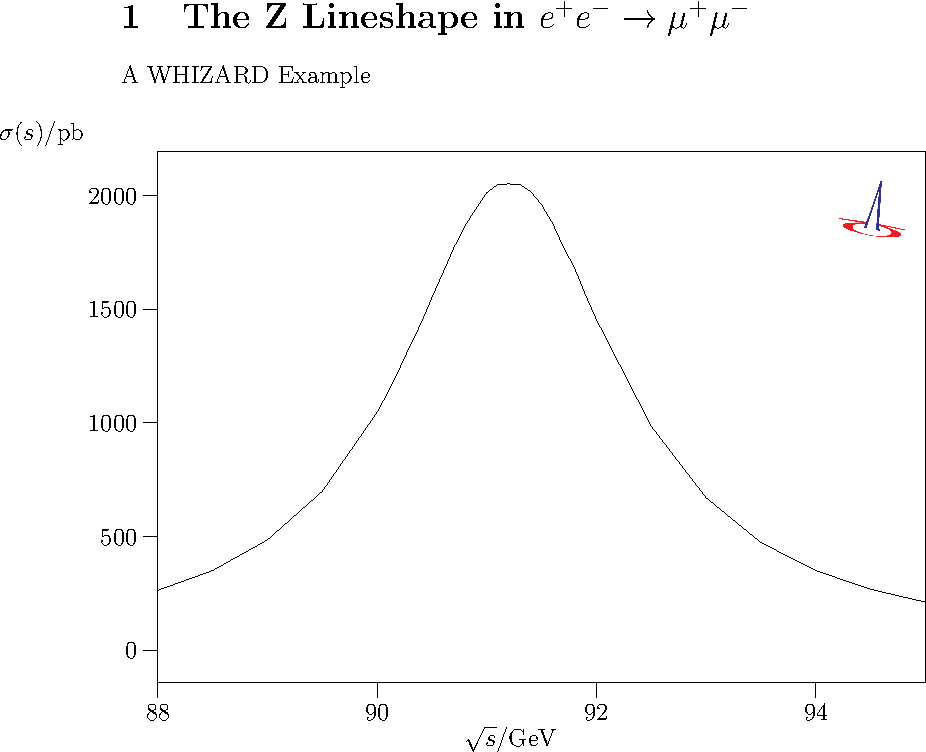
\includegraphics[width=.47\textwidth]{Z-lineshape_1}
  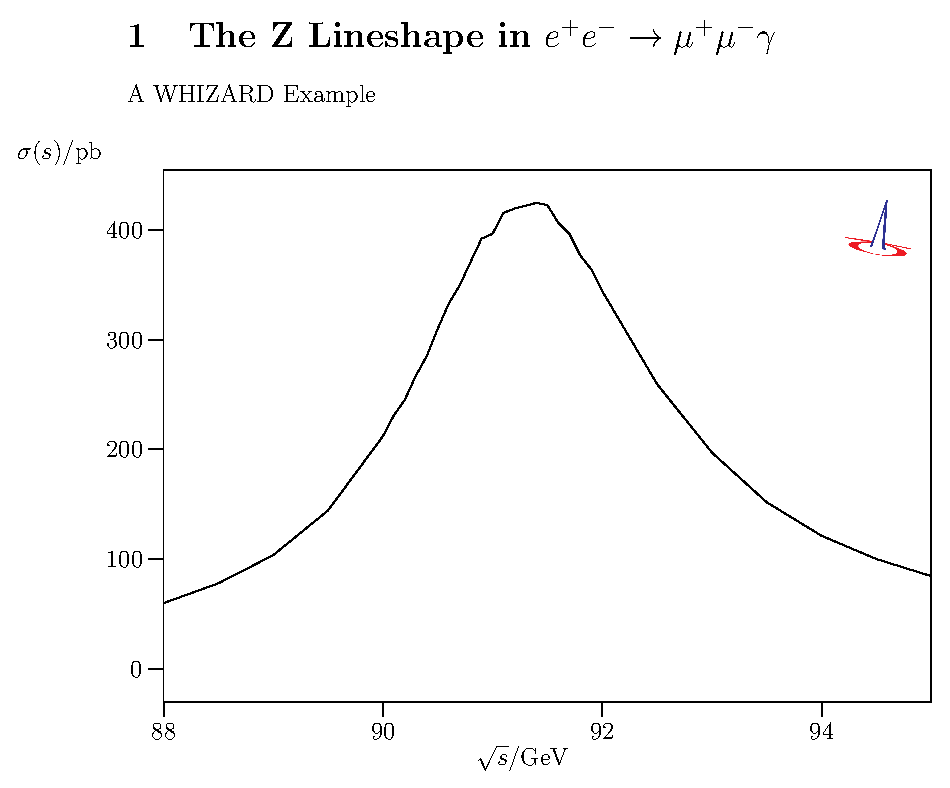
\includegraphics[width=.47\textwidth]{Z-lineshape_2}
\caption{\label{fig:zlineshape} $Z$ lineshape in the dimuon final
  state (left), and with an additional photon (right)}
\end{figure}
follow, and finally the same is done for the radiative process as
well. At the end of the SINDARIN script we compile the graphical
\whizard\ analysis and direct the data for the plots into the file
\ttt{Z-lineshape.dat}:
\begin{code}
compile_analysis { $out_file = "Z-lineshape.dat" }  
\end{code}
%$
In this case there is no event generation, but simply the cross
section values for the scan are dumped into a data file:
\begin{scriptsize}
\begin{Verbatim}[frame=single]
           $out_file = "Z-lineshape.dat"
           | Opening file 'Z-lineshape.dat' for output
           | Writing analysis data to file 'Z-lineshape.dat'
           | Closing file 'Z-lineshape.dat' for output
           | Compiling analysis results display in 'Z-lineshape.tex' 
\end{Verbatim}
\end{scriptsize}
%$
Fig.~\ref{fig:zlineshape} shows the graphical \whizard\ output of the
$Z$ lineshape in the dimuon final state from the scan on the left, and
the same for the radiative process with an additional photon on the
right. 

%%%%%%%%%%%%%%%

\section{$W$ pairs at LEP II}

This example which can be found as file \ttt{LEP\_cc10.sin} in the
\ttt{share/examples} directory, shows $W$ pair production in the
semileptonic mode at LEP II with its final energy of 209 GeV. Because
there are ten contributing Feynman diagrams, the process has been
dubbed CC10: charged current process with 10 diagrams. We work within
the Standard Model:
\begin{code}
  model = SM
\end{code}
Then the process is defined, where no flavor summation is done for the
jets here:
\begin{code}
  process cc10 = e1, E1 => e2, N2, u, D
\end{code}
A compilation statement is optional, and then we set the muon mass to
zero:
\begin{code}
  mmu = 0
\end{code}
The final LEP center-of-momentum energy of 209 GeV is set:
\begin{code}
  sqrts = 209 GeV
\end{code}
Then, we integrate the process:
\begin{code}
  integrate (cc10) { iterations = 12:20000 }
\end{code}
Running the SINDARIN file up to here, results in the output:
\begin{scriptsize}
\begin{Verbatim}[frame=single]
          | Process library 'default_lib': loading
          | Process library 'default_lib': ... success.
          SM.mmu =  0.000000000000E+00
          sqrts =  2.090000000000E+02
          | RNG: Initializing TAO random-number generator
          | RNG: Setting seed for random-number generator to 31255
          | Initializing integration for process cc10:
          | ------------------------------------------------------------------------
          | Process [scattering]: 'cc10'
          |   Library name  = 'default_lib'
          |   Process index = 1
          |   Process components:
          |     1: 'cc10_i1':   e-, e+ => mu-, numubar, u, dbar [omega]
          | ------------------------------------------------------------------------
          | Beam structure: [any particles]
          | Beam data (collision):
          |   e-  (mass = 5.1099700E-04 GeV)
          |   e+  (mass = 5.1099700E-04 GeV)
          |   sqrts = 2.090000000000E+02 GeV
          | Phase space: generating configuration ...
          | Phase space: ... success.
          | Phase space: writing configuration file 'cc10_i1.phs'
          | Phase space: 25 channels, 8 dimensions
          | Phase space: found 25 channels, collected in 7 groves.
          | Phase space: Using 25 equivalences between channels.
          | Phase space: wood
          Warning: No cuts have been defined.
          | OpenMP: Using 8 threads
          | Starting integration for process 'cc10'
          | Integrate: iterations = 12:20000
          | Integrator: 7 chains, 25 channels, 8 dimensions
          | Integrator: Using VAMP channel equivalences
          | Integrator: 20000 initial calls, 20 bins, stratified = T
          | Integrator: VAMP
          |=============================================================================|
          | It      Calls  Integral[fb]  Error[fb]   Err[%]    Acc  Eff[%]   Chi2 N[It] |
          |=============================================================================|
             1      19975  6.4714908E+02  2.17E+01    3.36    4.75*   2.33
             2      19975  7.3251876E+02  2.45E+01    3.34    4.72*   2.17
             3      19975  6.7746497E+02  2.39E+01    3.52    4.98    1.77
             4      19975  7.2075198E+02  2.41E+01    3.34    4.72*   1.76
             5      19975  6.5976152E+02  2.26E+01    3.43    4.84    1.46
             6      19975  6.6633310E+02  2.26E+01    3.39    4.79*   1.43
             7      19975  6.7539385E+02  2.29E+01    3.40    4.80    1.43
             8      19975  6.6754027E+02  2.11E+01    3.15    4.46*   1.41
             9      19975  7.3975817E+02  2.52E+01    3.40    4.81    1.53
            10      19975  7.2284275E+02  2.39E+01    3.31    4.68*   1.47
            11      19975  6.5476917E+02  2.18E+01    3.33    4.71    1.33
            12      19975  7.2963866E+02  2.54E+01    3.48    4.92    1.46
          |-----------------------------------------------------------------------------|
            12     239700  6.8779583E+02  6.69E+00    0.97    4.76    1.46    2.18  12
          |=============================================================================|
          | Time estimate for generating 10000 events: 0d:00h:01m:16s
          | Creating integration history display cc10-history.ps and cc10-history.pdf
\end{Verbatim}
\end{scriptsize}
\begin{figure}
  \centering
  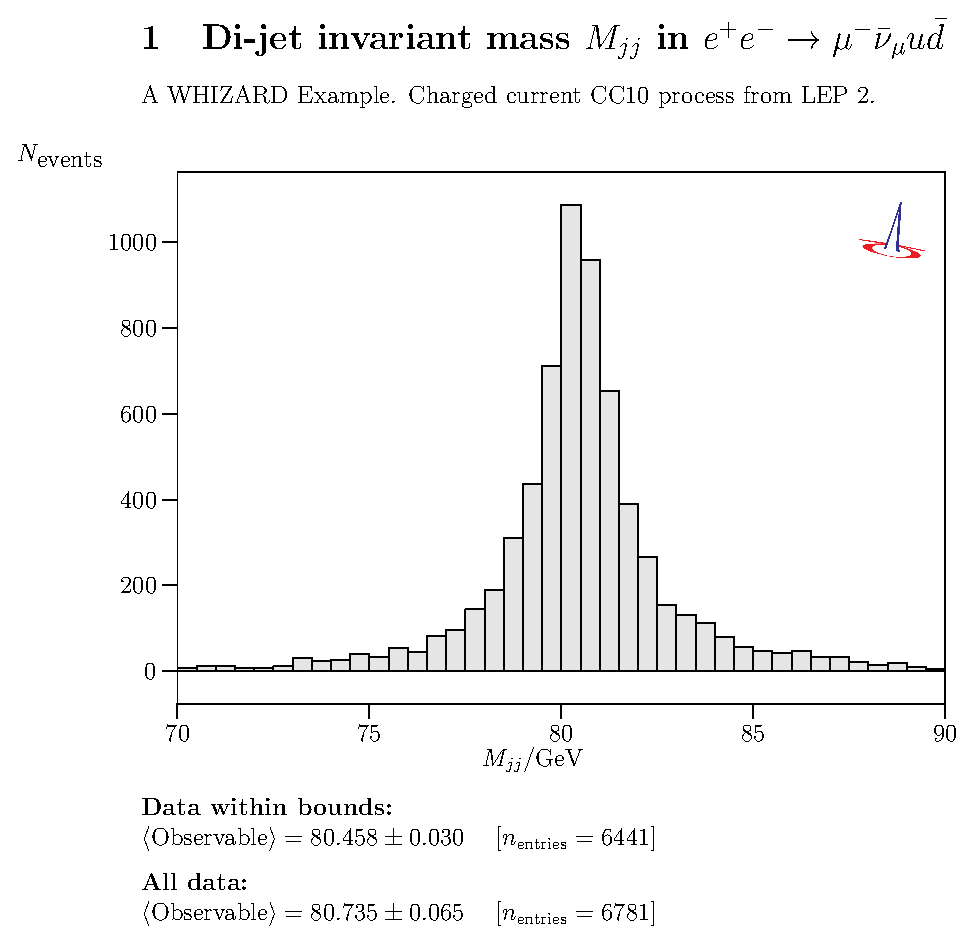
\includegraphics[width=.6\textwidth]{cc10_1} 
  \\\vspace{5mm}
  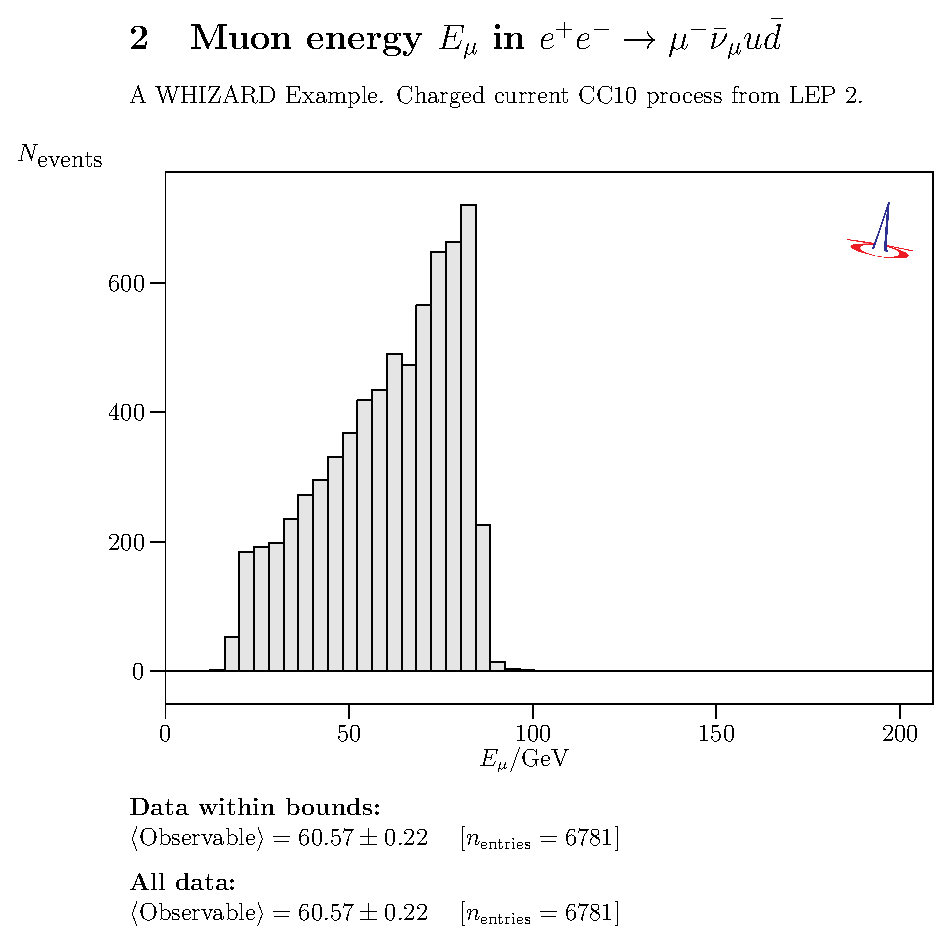
\includegraphics[width=.6\textwidth]{cc10_2}
  \caption{Histogram of the dijet invariant mass from the CC10 $W$
    pair production at LEP II, peaking around the $W$ mass (upper
    plot), and of the muon energy (lower plot).} 
  \label{fig:cc10}
\end{figure}
The next step is event generation. In order to get smooth
distributions, we set the integrated luminosity to 10
fb${}^{-1}$. (Note that LEP II in its final year 2000 had an
integrated luminosity of roughly 0.2 fb${}^{-1}$.)
\begin{code}
  luminosity = 10
\end{code}
With the simulated events corresponding to those 10 inverse femtobarn
we want to perform a \whizard\ analysis: we are going to plot the
dijet invariant mass, as well as the energy of the outgoing muon. For
the plot of the analysis, we define a description and label the $y$
axis:
\begin{code}
$description =
  "A WHIZARD Example.
   Charged current CC10 process from LEP 2."
$y_label = "$N_{\textrm{events}}$"  
\end{code}
We also use \LaTeX-syntax for the title of the first plot and the
$x$-label, and then define the histogram of the dijet invariant mass
in the range around the $W$ mass from 70 to 90 GeV in steps of half a
GeV: 
\begin{code}
$title = "Di-jet invariant mass $M_{jj}$ in $e^+e^- \to \mu^- \bar\nu_\mu u \bar d$"
$x_label = "$M_{jj}$/GeV"
histogram m_jets (70 GeV, 90 GeV, 0.5 GeV)  
\end{code}
And we do the same for the second histogram of the muon energy:
\begin{code}
$title = "Muon energy $E_\mu$ in $e^+e^- \to \mu^- \bar\nu_\mu u \bar d$"
$x_label = "$E_\mu$/GeV"
histogram e_muon (0 GeV, 209 GeV, 4)
\end{code}
Now, we define the \ttt{analysis} consisting of two \ttt{record}
statements initializing the two observables that are plotted as
histograms: 
\begin{code}
analysis = record m_jets (eval M [u,D]);
           record e_muon (eval E [e2])
\end{code}
At the very end, we perform the event generation
\begin{code}
simulate (cc10)  
\end{code}
and finally the writing and compilation of the analysis in a named
data file:
\begin{code}
compile_analysis { $out_file = "cc10.dat" }  
\end{code} 
This event generation part screen output looks like this:
\begin{scriptsize}
\begin{Verbatim}[frame=single]
          luminosity =  1.000000000000E+01
          $description = "A WHIZARD Example.
             Charged current CC10 process from LEP 2."
          $y_label = "$N_{\textrm{events}}$"
          $title = "Di-jet invariant mass $M_{jj}$ in $e^+e^- \to \mu^- \bar\nu_\mu u \bar d$"
          $x_label = "$M_{jj}$/GeV"
          $title = "Muon energy $E_\mu$ in $e^+e^- \to \mu^- \bar\nu_\mu u \bar d$"
          $x_label = "$E_\mu$/GeV"
          | Starting simulation for process 'cc10'
          | Simulate: using integration grids from file 'cc10_m1.vg'
          | RNG: Initializing TAO random-number generator
          | RNG: Setting seed for random-number generator to 9910
          | OpenMP: Using 8 threads
          | Simulation: using n_events as computed from luminosity value
          | Events: writing to raw file 'cc10.evx'
          | Events: generating 6830 unweighted, unpolarized events ...
          | Events: event normalization mode '1'
          |         ... event sample complete.
          Warning: Encountered events with excess weight: 39 events (  0.571 %)
          | Maximum excess weight = 1.027E+00
          | Average excess weight = 6.764E-04
          | Events: closing raw file 'cc10.evx'
          $out_file = "cc10.dat"
          | Opening file 'cc10.dat' for output
          | Writing analysis data to file 'cc10.dat'
          | Closing file 'cc10.dat' for output
          | Compiling analysis results display in 'cc10.tex'  
\end{Verbatim}
\end{scriptsize} %$
Then comes the \LaTeX\ output of the compilation of the graphical
analysis. Fig.~\ref{fig:cc10} shows the two histograms as the are
produced as result of the \whizard\ internal graphical analysis.

%%%%%%%%%%%%%%%

\section{Higgs search at LEP II}

This example can be found under the name \ttt{LEP\_higgs.sin} in the
\ttt{share/doc} folder of \whizard. It displays different search
channels for a very light would-be SM Higgs boson of mass 115 GeV at
the LEP II machine at its highest energy it finally achieved, 209 GeV.
First, we use the Standard Model:
\begin{code}
model = SM
\end{code}
Then, we define aliases for neutrinos, antineutrinos, light quarks and
light anti-quarks:
\begin{code}
alias n = n1:n2:n3
alias N = N1:N2:N3
alias q = u:d:s:c
alias Q = U:D:S:C  
\end{code}
Now, we define the signal process, which is Higgsstrahlung, 
\begin{code}
process zh = e1, E1 => Z, h  
\end{code}
the missing-energy channel,
\begin{code}
process nnbb = e1, E1 => n, N, b, B  
\end{code}
and finally the 4-jet as well as dilepton-dijet channels:
\begin{code}
process qqbb = e1, E1 => q, Q, b, B
process bbbb = e1, E1 => b, B, b, B
process eebb = e1, E1 => e1, E1, b, B
process qqtt = e1, E1 => q, Q, e3, E3
process bbtt = e1, E1 => b, B, e3, E3

compile  
\end{code}
and we compile the code. We set the center-of-momentum energy to the
highest energy LEP II achieved,
\begin{code}
sqrts = 209 GeV  
\end{code}
For the Higgs boson, we take the values of a would-be SM Higgs boson
with mass of 115 GeV, which would have had a width of a bit more than
3 MeV:
\begin{code}
mH = 115 GeV
wH = 3.228 MeV  
\end{code}
We take a running $b$ quark mass to take into account NLO corrections
to the $Hb\bar b$ vertex, while all other fermions are massless:
\begin{code}
mb = 2.9 GeV
me = 0
ms = 0
mc = 0  
\end{code}
\begin{scriptsize}
\begin{Verbatim}[frame=single]
           | Process library 'default_lib': loading
           | Process library 'default_lib': ... success.
           sqrts =  2.090000000000E+02
           SM.mH =  1.150000000000E+02
           SM.wH =  3.228000000000E-03
           SM.mb =  2.900000000000E+00
           SM.me =  0.000000000000E+00
           SM.ms =  0.000000000000E+00
           SM.mc =  0.000000000000E+00  
\end{Verbatim}
\end{scriptsize}
To avoid soft-collinear singular phase-space regions, we apply an
invariant mass cut on light quark pairs:
\begin{code}
cuts = all M >= 10 GeV [q,Q]  
\end{code}
Now, we integrate the signal process as well as the combined signal
and background processes:
\begin{code}
integrate (zh) { iterations = 5:5000}

integrate(nnbb,qqbb,bbbb,eebb,qqtt,bbtt) { iterations = 12:20000 }  
\end{code}
\begin{scriptsize}
\begin{Verbatim}[frame=single]
           | RNG: Initializing TAO random-number generator
           | RNG: Setting seed for random-number generator to 21791
           | Initializing integration for process zh:
           | ------------------------------------------------------------------------
           | Process [scattering]: 'zh'
           |   Library name  = 'default_lib'
           |   Process index = 1
           |   Process components:
           |     1: 'zh_i1':   e-, e+ => Z, H [omega]
           | ------------------------------------------------------------------------
           | Beam structure: [any particles]
           | Beam data (collision):
           |   e-  (mass = 0.0000000E+00 GeV)
           |   e+  (mass = 0.0000000E+00 GeV)
           |   sqrts = 2.090000000000E+02 GeV
           | Phase space: generating configuration ...
           | Phase space: ... success.
           | Phase space: writing configuration file 'zh_i1.phs'
           | Phase space: 1 channels, 2 dimensions
           | Phase space: found 1 channel, collected in 1 grove.
           | Phase space: Using 1 equivalence between channels.
           | Phase space: wood
           | Applying user-defined cuts.
           | OpenMP: Using 8 threads
           | Starting integration for process 'zh'
           | Integrate: iterations = 5:5000
           | Integrator: 1 chains, 1 channels, 2 dimensions
           | Integrator: Using VAMP channel equivalences
           | Integrator: 5000 initial calls, 20 bins, stratified = T
           | Integrator: VAMP
           |=============================================================================|
           | It      Calls  Integral[fb]  Error[fb]   Err[%]    Acc  Eff[%]   Chi2 N[It] |
           |=============================================================================|
              1       4608  1.6114109E+02  5.52E-04    0.00    0.00*  99.43
              2       4608  1.6114220E+02  5.59E-04    0.00    0.00   99.43
              3       4608  1.6114103E+02  5.77E-04    0.00    0.00   99.43
              4       4608  1.6114111E+02  5.74E-04    0.00    0.00*  99.43
              5       4608  1.6114103E+02  5.66E-04    0.00    0.00*  99.43
           |-----------------------------------------------------------------------------|
              5      23040  1.6114130E+02  2.53E-04    0.00    0.00   99.43    0.82   5
           |=============================================================================|
           [.....]  
\end{Verbatim}
\end{scriptsize}
\begin{figure}
  \centering
  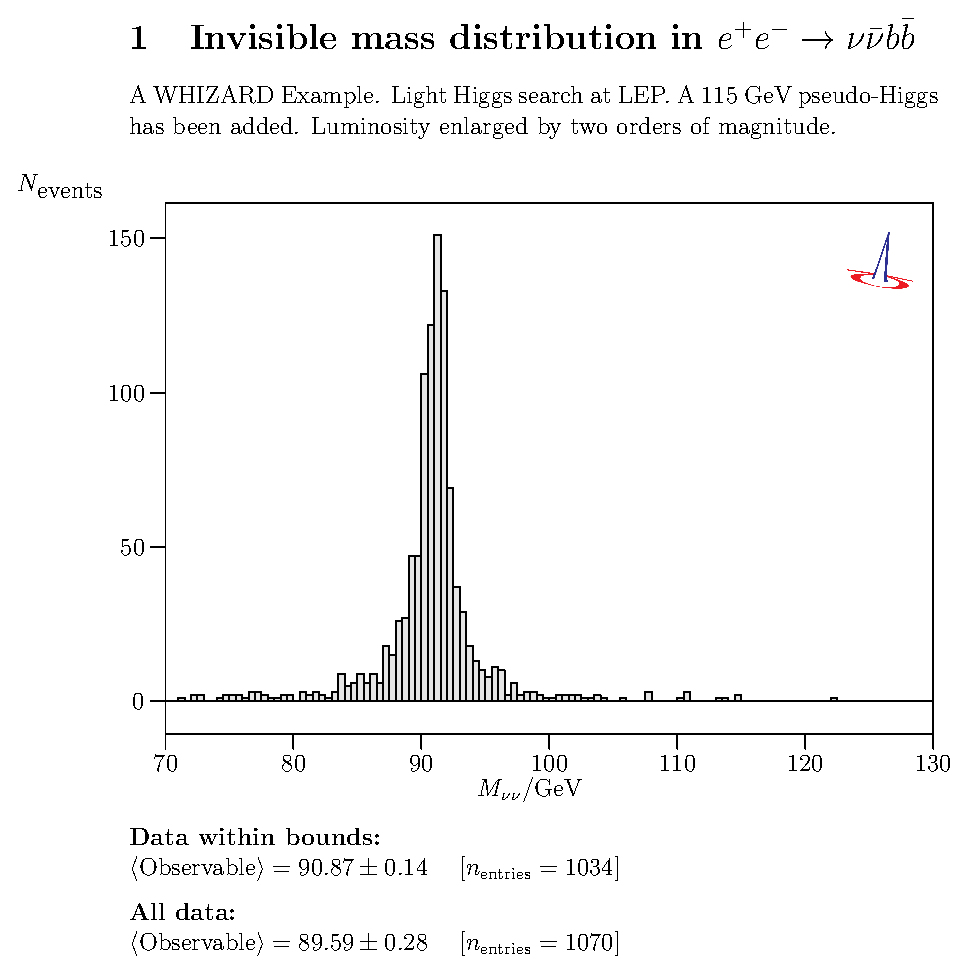
\includegraphics[width=.48\textwidth]{lep_higgs_1} 
  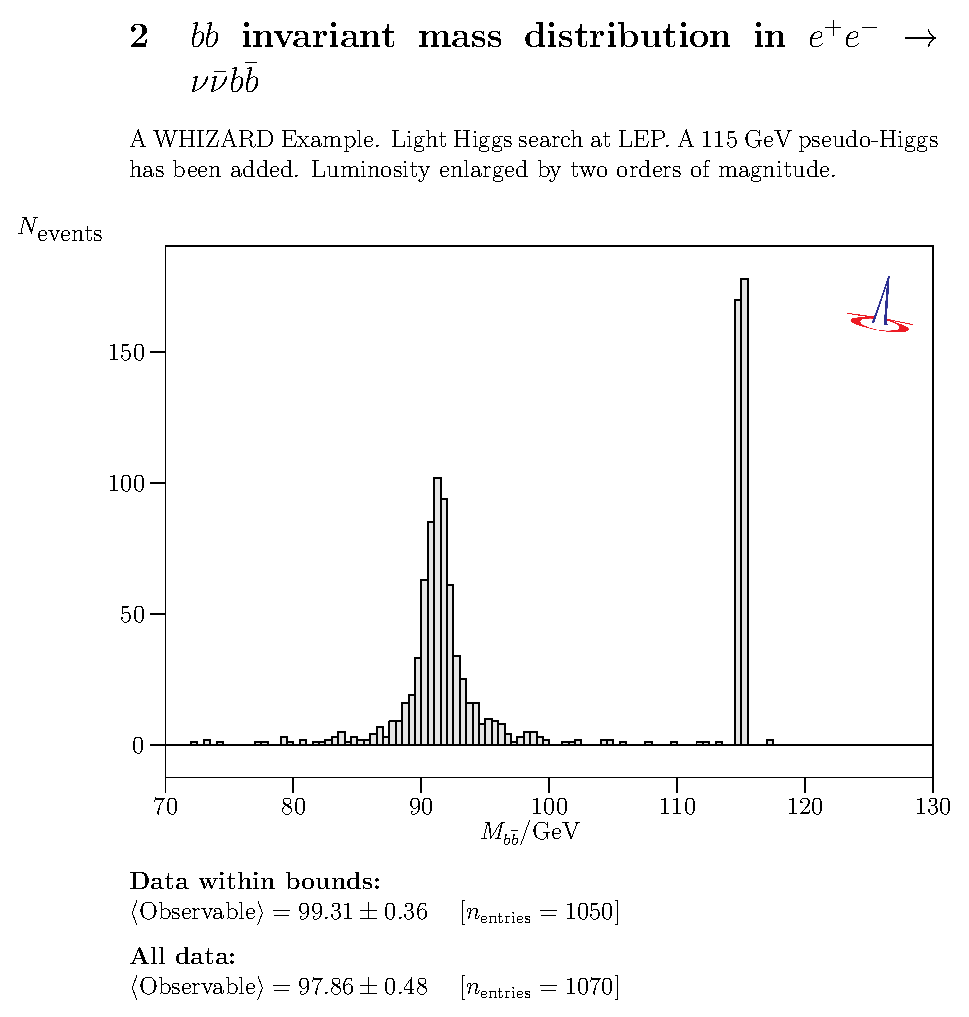
\includegraphics[width=.48\textwidth]{lep_higgs_2}
  \\\vspace{5mm}
  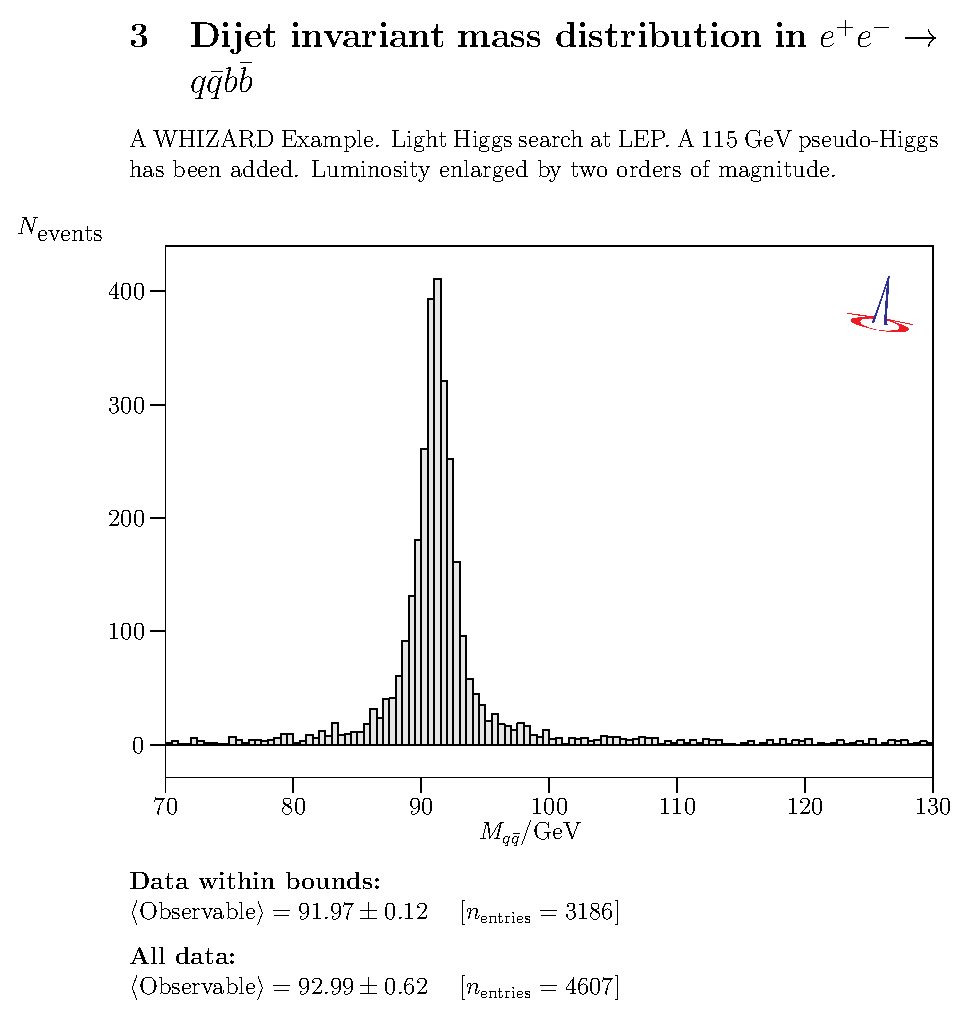
\includegraphics[width=.48\textwidth]{lep_higgs_3}
  \caption{Upper line: final state $bb + E_{miss}$, histogram of
    the invisible mass distribution (left), and of the di-$b$
    distribution (right). Lower plot: light dijet distribution in the 
    $bbjj$ final state.}
  \label{fig:lep_higgs}
\end{figure}
Because the other integrations look rather similar, we refrain from
displaying them here, too. As a next step, we define titles,
descriptions and axis labels for the histograms we want to
generate. There are two of them, one os the invisible mass
distribution, the other is the di-$b$-jet invariant mass. Both
histograms are taking values between 70 and 130 GeV with 
bin widths of half a GeV:
\begin{code}
$description =   
  "A WHIZARD Example. Light Higgs search at LEP. A 115 GeV pseudo-Higgs 
    has been added. Luminosity enlarged by two orders of magnitude."
$y_label = "$N_{\textrm{events}}$"

$title = "Invisible mass distribution in $e^+e^- \to \nu\bar\nu b \bar b$"
$x_label = "$M_{\nu\nu}$/GeV"
histogram m_invisible (70 GeV, 130 GeV, 0.5 GeV)

$title = "$bb$ invariant mass distribution in $e^+e^- \to \nu\bar\nu b \bar b$"
$x_label = "$M_{b\bar b}$/GeV"
histogram m_bb (70 GeV, 130 GeV, 0.5 GeV)  
\end{code}
The analysis is initialized by defining the two records for the
invisible mass and the invariant mass of the two $b$ jets:
\begin{code}
analysis = record m_invisible (eval M [n,N]);
           record m_bb (eval M [b,B])  
\end{code}
In order to have enough statistics, we enlarge the LEP integrated
luminosity at 209 GeV by more than two orders of magnitude:
\begin{code}
luminosity = 10  
\end{code}
We start event generation by simulating the process with two $b$ jets
and two neutrinos in the final state:
\begin{code}
simulate (nnbb)  
\end{code}
As a third histogram, we define the dijet invariant mass of two light
jets: 
\begin{code}
$title = "Dijet invariant mass distribution in $e^+e^- \to q \bar q b \bar b$"
$x_label = "$M_{q\bar q}$/GeV"
histogram m_jj (70 GeV, 130 GeV, 0.5 GeV)  
\end{code}
Then we simulate the 4-jet process defining the light-dijet
distribution as a local record:
\begin{code}
simulate (qqbb) { analysis = record m_jj (eval M / 1 GeV [combine [q,Q]]) }  
\end{code}
Finally, we compile the analysis,
\begin{code}
compile_analysis { $out_file = "lep_higgs.dat" }  
\end{code}
\begin{scriptsize}
\begin{Verbatim}[frame=single]
           | Starting simulation for process 'nnbb'
           | Simulate: using integration grids from file 'nnbb_m1.vg'
           | RNG: Initializing TAO random-number generator
           | RNG: Setting seed for random-number generator to 21798
           | OpenMP: Using 8 threads
           | Simulation: using n_events as computed from luminosity value
           | Events: writing to raw file 'nnbb.evx'
           | Events: generating 1070 unweighted, unpolarized events ...
           | Events: event normalization mode '1'
           |         ... event sample complete.
           Warning: Encountered events with excess weight: 207 events ( 19.346 %)
           | Maximum excess weight = 1.534E+00
           | Average excess weight = 4.909E-02
           | Events: closing raw file 'nnbb.evx'
           $title = "Dijet invariant mass distribution in $e^+e^- \to q \bar q b \bar b$"
           $x_label = "$M_{q\bar q}$/GeV"
           | Starting simulation for process 'qqbb'
           | Simulate: using integration grids from file 'qqbb_m1.vg'
           | RNG: Initializing TAO random-number generator
           | RNG: Setting seed for random-number generator to 21799
           | OpenMP: Using 8 threads
           | Simulation: using n_events as computed from luminosity value
           | Events: writing to raw file 'qqbb.evx'
           | Events: generating 4607 unweighted, unpolarized events ...
           | Events: event normalization mode '1'
           |         ... event sample complete.
           Warning: Encountered events with excess weight: 112 events (  2.431 %)
           | Maximum excess weight = 8.875E-01
           | Average excess weight = 4.030E-03
           | Events: closing raw file 'qqbb.evx'
           $out_file = "lep_higgs.dat"
           | Opening file 'lep_higgs.dat' for output
           | Writing analysis data to file 'lep_higgs.dat'
           | Closing file 'lep_higgs.dat' for output
           | Compiling analysis results display in 'lep_higgs.tex'  
\end{Verbatim}
\end{scriptsize}
The graphical analysis of the events generated by \whizard\ are shown
in Fig.~\ref{fig:lep_higgs}. In the upper left, the invisible mass
distribution in the $b\bar b + E_{miss}$ state is shown, peaking
around the $Z$ mass. The upper right shows the $M(b\bar b)$
distribution in the same final state, while the lower plot has the
invariant mass distribution of the two non-$b$-tagged (light) jets in
the $bbjj$ final state. The latter shows only the $Z$
peak, while the former exhibits the narrow would-be 115 GeV Higgs
state. 

%%%%%%%%%%%%%%%

\section{Deep Inelastic Scattering at HERA}

%%%%%%%%%%%%%%%

\section{$W$ endpoint at LHC}

%%%%%%%%%%%%%%%

\section{SUSY Cascades at LHC}

%%%%%%%%%%%%%%%

\section{Polarized $WW$ at ILC}

%%%%%%%%%%%%%%%%%%%%%%%%%%%%%%%%%%%%%%%%%%%%%%%%%%%%%%%%%%%%%%%%%%%%%%%%

\chapter{Technical details -- Advanced Spells}
\label{chap:tuning}

\section{Efficiency and tuning}

Since massless fermions and vector bosons (or almost massless states
in a certain approximation) lead to restrictive selection rules for
allowed helicity combinations in the initial and final state. To make
use of this fact for the efficiency of the \whizard\ program, we are
applying some sort of heuristics: \whizard\ dices events into all
combinatorially possible helicity configuration during a warm-up
phase. The user can specify a helicity threshold which sets the number
of zeros \whizard\ should have got back from a specific helicity
combination in order to ignore that combination from now on. By that
mechanism, typically half up to more than three quarters of all
helicity combinations are discarded (and hence the corresponding
number of matrix element calls). This reduces calculation time up to
more than one order of magnitude. \whizard\ shows at the end of the
integration those helicity combinations which finally contributed to
the process matrix element.

Note that this list -- due to the numerical heuristics -- might very
well depend on the number of calls for the matrix elements per
iteration, and also on the corresponding random number seed.  

%%%%%%%%%%%%%%%%%%%%%%%%%%%%%%%%%%%%%%%%%%%%%%%%%%%%%%%%%%%%%%%%%%%%%%%%
%%%%%%%%%%%%%%%%%%%%%%%%%%%%%%%%%%%%%%%%%%%%%%%%%%%%%%%%%%%%%%%%%%%%%%%%

\chapter{New External Physics Models}
\label{chap:extmodels}

Its never possible to include all incarnations of physics models that
can be described by the maybe weirdest form of a quantum field theory
in a tailor-made implementation within a program like \whizard. Users
clearly want to be able to use their own special type of model; in
order to do so there are external tools to translate models described
by their field content and Lagrangian densities into Feynman rules and
make them available in an event generator like \whizard. In this
chapter, we describe the interfaces to two such external models,
\sarah\ and \FeynRules. 

The \FeynRules\ interface had been started already for the legacy
version \whizard\ttt{1} (where it had to be downloaded from 
\url{http://projects.hepforge.org/whizard} as a separate package), but
for the \whizard\ttt{two} release series it has been included in the
\FeynRules\ package (from their version v1.6.0 on). Note that there
was a regression for the usage of external models (from either \sarah\
or \FeynRules) in the first release of series v2.2, v2.2.0. This has
been fixed in all upcoming versions.

%%%%%%%%%%%%%%%

\section{New physics models via \sarah}
\sarah~\cite{Staub:2008uz,Staub:2009bi,Staub:2010jh,Staub:2012pb,Staub:2013tta}
is a \Mathematica~\cite{mathematica} package which 
derives for a given model the 
minimum conditions of the vacuum, the mass matrices, and vertices at tree-level
as well as expressions for the one-loop corrections for all masses and the 
full two-loop renormalization group equations (RGEs). The vertices can be exported 
to be used with \whizard/\oMega. All other information can be used to generate
\fortran\ source code for the RGE solution tool and spectrum generator
\spheno~\cite{Porod:2003um,Porod:2011nf}  to get a spectrum generator
for any model. The  
advantage is that \spheno\ calculates a consistent set of parameters (couplings, 
masses, rotation matrices, decay widths) which can be used as input for \whizard. 
\sarah\ and \spheno\ can be also downloaded from the \ttt{HepForge} server:
\begin{center}
\url{http://sarah.hepforge.org} \\
\url{http://spheno.hepforge.org}
\end{center}


\subsection{\whizard/\oMega\ model files from \sarah}

\subsubsection{Generating the model files}

Here we are giving only the information relevant to generate models
for \whizard. For more details about the installation of \sarah\ and
an exhaustion documentation about its usage, confer the \sarah\
manual. 

To generate the model files for \whizard/\oMega\ with \sarah, a 
new \Mathematica\ session has to be started. \sarah\ is loaded via
\begin{code}
<<SARAH-4.2.1/SARAH.m; 
\end{code}
if \sarah\ has been stored in the applications directory of
\Mathematica. Otherwise, the full path has to be given
\begin{code}
<<[Path_to_SARAH]/SARAH.m;
\end{code}
To get an overview which models are delivered with \sarah, the command \verb"ShowModels"
can be used. As an example, we use in the following the triplet
extended MSSM (TMSSM) and initialize it in \sarah\ via
\begin{code}
Start["TMSSM"]; 
\end{code}
Finally, the output intended for \whizard/\oMega\ is started via
\begin{code}
MakeWHIZARD[Options]
\end{code}
The possible options of the \verb"MakeWHIZARD" command are
\begin{enumerate}
  \item \verb"WriteOmega", with values: \verb"True" or \verb"False", default:
    \verb"True" \\
    Defines if the model files for \oMega\ should be written
  \item \verb"WriteWHIZARD", with values: \verb"True" or \verb"False",
    default: \verb"True" \\
    Defines if the model files for \whizard\ should be written
  \item \verb"Exclude", with values: list of generic type, Default:
    \verb"{SSSS}" \\ 
    Defines which generic vertices are {\em not} exported to the model
    file 
  \item \verb"WOModelName", with values: string, default: name of the
    model in \sarah\ followed by \verb"_sarah"  \\ 
    Gives the possibility to change the model name
  \item \verb"MaximalCouplingsPerFile", with values: integer, default:
    \ttt{150} \\
    Defines the maximal number of couplings written per file
  \item \verb"Version", with values: formatted number, Default:
    \verb"2.2.1"~\footnote{Due to a regression in \whizard\ version
      v2.2.0, \sarah\ models cannot be successfully linked within 
      that version. Hence, the default value here has been set to
      version number 2.2.1}, \\
    Defines the version of \whizard\ for which the model file is generated
\end{enumerate}
All options and the default values are also shown in the 
\Mathematica\ session via \newline\verb"Options[MakeWHIZARD]".

\subsubsection{Using the generated model files with \whizard}

After the interface has completed evaluation, the generated files can
be found in the subdirectory \verb"WHIZARD_Omega" of {\sarah}s output
directory. In order to use it the generated code must be compiled and
installed. For this purpose, open a terminal, enter the output directory 
\begin{code}
<PATH_to_SARAH>/Output/TMSSM/EWSB/WHIZARD_Omega/ 
\end{code}
and run
%
\begin{code}
./configure
make install
\end{code} 
%
By default, the last command installs the compiled model into \verb".whizard"
in current user's home directory where it is automatically picked up by
\whizard. Alternative installation paths can be specified using the
\verb"--prefix" option to \whizard.
%
\begin{code}
./configure --prefix=/path/to/installation/prefix
\end{code} 
%
If the files are installed into the \whizard\
installation prefix, the program will also pick them up automatically, while
{\whizard}'s \verb"--localprefix" option must be used to communicate any other
choice to \whizard. In case \whizard\ is not available in the binary search
path, the \verb"WO_CONFIG" environment variable can be used to point
\verb"configure" to the binaries
%
\begin{code}
./configure WO_CONFIG=/path/to/whizard/binaries
\end{code} 
%
More information on the available options and their syntax can be obtained with
the
\verb"--help" option.

After the model is compiled it can be used in \whizard\ as
\begin{code}
model = tmssm_sarah 
\end{code}



\subsection{Linking \spheno\ and \whizard}
As mentioned above, the user can also use \spheno\ to generate spectra
for its models. This is done by means of \fortran\ code for \spheno,
exported from \sarah.  To do so, the user has to apply the command
\verb"MakeSPheno[]". For more details  
about the options of this command and how to compile and use the \spheno\ output,
we refer to the \sarah\ manual. \\
As soon as the \spheno\ version for the given model is ready it can be used to
generate files with all necessary numerical values for the parameters in a format
which is understood by \whizard. For this purpose, the corresponding flag in the 
Les Houches input file of \spheno\ has to be turned on:
\begin{code}
Block SPhenoInput   # SPheno specific input
...
75 1               # Write WHIZARD files
\end{code}
Afterwards, \spheno\ returns not only the spectrum file in the
standard SUSY Les Houches accord (SLHA) format (for more details about
the SLHA and the \whizard\ SLHA interface cf. Sec.~\ref{sec:slha}), 
but also an additional file called \verb"WHIZARD.par.TMSSM" for our example. 
This file can be used
in the SINDARIN input file via
\begin{code}
include ("WHIZARD.par.TMSSM") 
\end{code}

%%%%%

\subsection{BSM Toolbox}

A convenient way to install \sarah\ together with \whizard, \spheno\
and some  other codes are the \ttt{BSM Toolbox} scripts
\footnote{Those script have been published  
under the name SUSY Toolbox but \sarah\ is with version 4 no longer
restricted to SUSY models}~\cite{Staub:2011dp}. These scripts are
available at 
\begin{center}
 \url{http://projects.hepforge.org/sarah/Toolbox.html}
\end{center}
The \ttt{Toolbox} provides two scripts. First, the \verb"configure" script is
used via
\begin{code} 
toolbox-src-dir> mkdir build
toolbox-src-dir> cd build
toolbox-src-dir> ../configure
\end{code}
%
The  \verb"configure" script checks for the requirements of the
different packages and downloads all codes. All downloaded archives will
be placed in the \verb"tarballs" subdirectory of the directory containing the
\verb"configure" script.
Command line options can be used to disable specific packages and to point the
script to custom locations of compilers and of the \Mathematica\ kernel; a full
list of those can be obtained by calling \verb"configure" with the \verb"--help"
option.

After \verb"configure" finishes successfully, \verb"make" can be called to build
all configured packages
%
\begin{code} 
toolbox-build-dir> make
\end{code}

\verb"configure" creates also the second script which automates the implementation
of a new model into all packages. The \verb"butler" script takes as argument the 
name of the model in \sarah, e.g.
\begin{code} 
> ./butler TMSSM
\end{code}
The \verb"butler" script runs \sarah\ to get the output in the same
form as the \whizard/\oMega\
model files and the code for \spheno. Afterwards, it installs the 
model in all packages and compiles the new \whizard/\oMega\ model
files as well as the new \spheno\ module. 

%%%%%
\newpage

\section{New physics models via \FeynRules}

In this section, we present the interface between the external tool
\FeynRules\ \cite{Christensen:2008py,Christensen:2009jx,Duhr:2011se}
and \whizard. \FeynRules\ is a 
\Mathematica~\cite{mathematica} package that allows to derive
Feynman rules from any perturbative quantum field theory-based Lagrangian 
in an automated way. It can be downloaded from
\begin{center}
  \url{http://feynrules.irmp.ucl.ac.be/}
\end{center}
The input provided by the user is threefold and consists 
of the Lagrangian defining the model, together with the definitions of
all the 
particles and parameters that appear in the model. 
Once this information is provided, \FeynRules\ can perform basic checks 
on the sanity of the implementation (e.g. hermiticity, normalization
of the quadratic terms), and finally computes all the interaction
vertices associated  with the model and store them in an internal
format for later processing. After the Feynman rules have been
obtained, \FeynRules\ can export the interaction vertices to \whizard\
via a dedicated interface~\cite{Christensen:2010wz}. The interface
checks whether all the vertices are compliant with the structures
supported by \whizard's 
matrix element generator \oMega, and discard them in the case 
they are not supported. The output of the interface consists of a set
of files organized in a single directory which can be injected into
\whizard/\oMega\ and used as any other built-in models. Together with
the model files, a framework is created which allows to communicate
the new models to \whizard\ in a well defined way, after which 
step the model can be used exactly like the built-in ones.
This specifically means that the user is not required to
manually modify the code of \whizard/\oMega, the models created by the
interface can be used directly without any further user intervention.
We first describe the installation and general usage of the interface,
and then list the general properties like the supported particle
types, color quantum numbers and Lorentz structures as well as types
of gauge interactions.

%%%%%%%%%%%%%%%%%%%%%%%%%%%%%%%%%%%%%%%%%%%%%%%%%%%%%%%%%%%%%%%%%%%%%%%%

\subsection{Installation and Usage of the \whizard-\FeynRules\ interface}
\label{sec:interface-usage}

\paragraph{{\bf Installation and basic usage:}}
%
From \FeynRules\ version 1.6.0 onward, the interface to \whizard\ is
part of the \FeynRules\ distribution\footnote{Note that though the
  main interface of \FeynRules\ to \whizard\ is for the most recent
  \whizard\ release, but also the legacy branch 
  \whizard\ttt{1} is supported.}. In addition, the latest version
of the interface can be downloaded from the \whizard\ homepage on
\ttt{HepForge}. There you can also find an installer that can be used
to inject the interface into an existing \FeynRules\
installation (which allows to use the interface with the \FeynRules\
release series1.4.x where it is not part of the package). 

Once installed, the interface can be called and used in the same way
\FeynRules' other interfaces described
in~\cite{Christensen:2008py}. The details of how to install and use 
\FeynRules\ itself can be found
there,~\cite{Christensen:2008py,Christensen:2009jx,Duhr:2011se}. Here, 
we only describe how to use the interface to inject new models into
\whizard.  For example, once the  \FeynRules\ environment has been
initialized and a model has been loaded, the command
\begin{code}
  WriteWOOutput[L]
\end{code}
will call the \texttt{FeynmanRules} command to extract the Feynman
rules from the Lagrangian \texttt{L}, translate them together with the
model data and finally write the files necessary for using the model
within \whizard\ to an output directory (the name of which is inferred
from the model name by default). Options can be added for further
control over the translation process (see
Sec.~\ref{app:interface-options}). Instead of using a Lagrangian, it
is also possible to call the interface on a pure vertex list. For
example, the following command 
\begin{code}
  WriteWOOutput[Input -> list]
\end{code}
will directly translate the vertex list \texttt{list}. Note that this 
vertex list must be given in flavor-expanded form in order for the
interface to process it correctly. 

The interface also supports the \texttt{WriteWOExtParams} command
described in~\cite{Christensen:2008py}. Issuing 
\begin{code}
  WriteWOExtParams[filename]
\end{code}
will write a list of all the external parameters to
\texttt{filename}. This is done in the form of a SINDARIN 
script. The only option accepted by the command above is the target
version of \whizard, set by the option \texttt{WOWhizardVersion}.

During execution, the interface will print out a series of
messages. It is highly advised to carefully read through this output
as it not only summarizes the settings and the location of the output
files, but also contains information on any skipped vertices or
potential incompatibilities of the model with \whizard. 

After the interface has run successfully and written the model files to the
output directory, the model must be imported into \whizard. For doing
so, the model files have to be compiled and can then be installed 
independently of \whizard. In the simplest scenario, assuming that the
output directory is the current working directory and that the
\whizard\ binaries can be found in the current \texttt{\$\{PATH\}},
the installation is performed by simply executing
\begin{code}
./configure~\&\&~make clean~\&\&~make install
\end{code}

This will compile the model and install it into the directory
\texttt{\$\{HOME\}/.whizard}, making it fully available to \whizard\
without any further intervention. The build system can be adapted to
more complicated cases through several options to the
\texttt{configure} which are listed in the \texttt{INSTALL} file
created in the output directory. A detailed explanation of all options 
can be found in Sec.~\ref{app:interface-options}.

\paragraph{\bf Supported fields and vertices:}

The following fields are currently supported by the interface:
scalars, Dirac and Majorana fermions, vectors and symmetric tensors.
The set of accepted operators, the full list of which can be found in
Tab.~\ref{tab-operators}, is a subset of all the operators supported
by \oMega. While still limited, this list is sufficient for a large
number of BSM models. In addition, a future version of
\whizard/\oMega\ will support the definition of completely general  
Lorentz structures in the model, allowing the interface to
translate all interactions handled by \FeynRules. This will be done by
means of a parser within \oMega\ of the \ttt{UFO} file format for
model files from \FeynRules.
 
\begin{table*}[!t]
\centerline{\begin{tabular}{|c|c|}
\hline Particle spins & Supported Lorentz structures \\\hline\hline
FFS & \parbox{0.7\textwidth}{\raggedright
   All operators of dimension four are supported.
\strut}\\\hline
FFV & \parbox[t]{0.7\textwidth}{\raggedright
   All operators of dimension four are
   supported.
\strut}\\\hline
SSS & \parbox{0.7\textwidth}{\raggedright
   All dimension three interactions are supported.
\strut}\\\hline
SVV & \parbox[t]{0.7\textwidth}{\raggedright
   Supported operators:\\
   \mbox{}\hspace{5ex}$\begin{aligned}
      \text{dimension 3:} & \quad\mathcal{O}_3 = V_1^\mu V_{2\mu}\phi \mbox{}\\
      \text{dimension 5:} & \quad\mathcal{O}_5 = \phi
         \left(\partial^\mu V_1^\nu - \partial^\nu V_1^\mu\right)
         \left(\partial_\mu V_{2\nu} - \partial_\nu V_{2\mu}\right)
   \end{aligned}$\\
Note that $\mathcal{O}_5$ generates the effective gluon-gluon-Higgs couplings obtained by integrating out heavy quarks.
\strut}\\\hline
SSV & \parbox[t]{0.7\textwidth}{\raggedright
   $\left(\phi_1\partial^\mu\phi_2 - \phi_2\partial^\mu\phi_1\right)V_\mu\;$
   type interactions are supported.
\strut}\\\hline
SSVV & \parbox{0.7\textwidth}{\raggedright
   All dimension four interactions are supported.
\strut}\\\hline
SSSS & \parbox{0.7\textwidth}{\raggedright
   All dimension four interactions are supported.
\strut}\\\hline
VVV & \parbox[t]{0.7\textwidth}{\raggedright
   All parity-conserving dimension four operators are supported, with
   the restriction that non-gauge interactions may be split into
   several vertices and can only be handled if all three fields are
   mutually different.\strut 
\strut}\\\hline
VVVV & \parbox[t]{0.7\textwidth}{\raggedright
   All parity conserving dimension four operators are supported. 
\strut}\\\hline
TSS, TVV, TFF & \parbox[t]{0.7\textwidth}{\raggedright
   The three point couplings in the Appendix of Ref.\
   \cite{Han:1998sg} are supported. 
\strut}\\\hline
\end{tabular}}
\caption{All Lorentz structures currently supported by the
  \whizard-\FeynRules\ interface, sorted with respect to the spins of
  the particles. ``S'' stands for scalar, ``F'' for fermion (either 
  Majorana or Dirac) and ``V'' for vector.} 
\label{tab-operators}
\end{table*}

\paragraph{\bf Color:}
%
Color is treated in \oMega\ in the color flow decomposition,
with the flow structure being implicitly determined from
the representations of the particles present at the vertex. Therefore, the
interface has to strip the color structure from the vertices derived by
\FeynRules\ before writing them out to the model files.
While this process is straightforward for all color structures which
correspond only to a single flow assignment, vertices with several
possible flow configurations must be treated with care in order to
avoid mismatches between the flows assigned by \oMega\ and those
actually encoded in the couplings. To this end, the interface derives
the color flow decomposition from the color structure determined by
\FeynRules\ and rejects all vertices which would lead to a wrong flow
assignment by \oMega\ (these rejections are accompanied by warnings
from the interface)\footnote{For the old \whizard\ttt{1} legacy
  branch, there was a maximum number of external color flows that had
  to explicitly specified. Essentially, this is $n_8 - \frac{1}{2}n_3$
  where $n_8$ is the maximum number of external color octets and $n_3$
  is the maximum number of external triplets and antitriplets. This
  can be set in the \whizard/\FeynRules\ interface by the
  \texttt{WOMaxNcf} command, whose default is \ttt{4}.}.

At the moment, the $SU(3)_C$ representations supported by  
both \whizard\ and the interface are singlets ($1$), triplets ($3$),
antitriplets ($\bar{3}$) and octets ($8$). Tab.~\ref{tab:su3struct}
shows all combinations of these representations which can 
form singlets together with the support status of the respective color
structures in \whizard\ and the interface. Although the supported
color structures do not comprise all possible singlets, the list is
sufficient for a large number of SM extensions. Furthermore, a future
revision of \whizard/\oMega\ will allow for explicit color flow
assignments, thus removing most of the current restrictions.

\begin{table*}
\centerline{\begin{tabular}{|c|c|}
\hline $SU(3)_C$ representations &
   Support status
\\\hline\hline
\parbox[t]{0.2\textwidth}{
   \centerline{\begin{tabular}[t]{lll}
   $111,\quad$ & $\bar{3}31,\quad$ & $\bar{3}38,$ \\
   $1111,$ & $\bar{3}311,$ & $\bar{3}381$
   \end{tabular}}} &
\parbox[t]{0.7\textwidth}{\raggedright\strut Fully supported by the interface\strut}
\\\hline
$888,\quad 8881$ &
\parbox{0.7\textwidth}{\raggedright\strut Supported only if at least two of the octets
are identical particles.\strut}
\\\hline
$881,\quad 8811$ &
\parbox{0.7\textwidth}{\raggedright\strut Fully supported by the
  interface\footnote{%
    Not available in version 1.95 and earlier. Note that in order to
    use such couplings in 1.96/97, the 
    \oMega\ option \texttt{2g} must be added to the process definition 
    in \texttt{whizard.prc}.}.\strut} 
\\\hline
$\bar{3}388$ &
\parbox{0.7\textwidth}{\raggedright\strut Supported only if the octets
  are identical 
particles.\strut}
\\\hline
$8888$ &
\parbox{0.7\textwidth}{\raggedright\strut The only supported flow structure is
\begin{equation*}
\parbox{21mm}{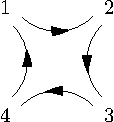
\includegraphics{flow4}}\cdot\;\Gamma(1,2,3,4)
   \quad+\quad \text{all acyclic permutations}
\end{equation*}
where $\Gamma(1,2,3,4)$ represents the Lorentz structure associated with the
first flow.\strut}
\\\hline
\parbox[t]{0.2\textwidth}{
   \centerline{\begin{tabular}[t]{lll}
   $333,\quad$ & $\bar{3}\bar{3}\bar{3},\quad$ & $3331$\\
   $\bar{3}\bar{3}\bar{3}1,$ & $\bar{3}\bar{3}33$
   \end{tabular}}} &
\parbox[t]{0.7\textwidth}{\raggedright\strut Unsupported (at the
  moment)\strut}
\\\hline
\end{tabular}}
\caption{All possible combinations of three or four $SU(3)_C$
representations supported by \FeynRules\ which can be used to build singlets,
together with the support status of the corresponding color structures in
\whizard\ and the interface.}
\label{tab:su3struct}
\end{table*}

\paragraph{\bf Running $\alpha_S$:}

While a running strong coupling is fully supported by the interface, a
choice has to be made which quantities are to be reevaluated when the
strong coupling is evolved. By default \texttt{aS}, \texttt{G} (see
Ref.~\cite{Christensen:2008py} for the nomenclature regarding 
the QCD coupling) and any vertex factors depending on them are evolved.
The list of internal parameters that are to be recalculated (together
with the vertex factors depending on them) can be
extended (beyond \texttt{aS} and \texttt{G}) by using
the option \texttt{WORunParameters} when calling the
interface~\footnote{As the legacy branch, \whizard\ttt{1}, does not
  support a running strong coupling, this is also vetoed by the
  interface when using \whizard \ttt{1.x}.}.

\paragraph{\bf Gauge choices:}
\label{sec:gauge-choices}

The interface supports the unitarity, Feynman and $R_\xi$ gauges. The choice of
gauge must be communicated to the interface via the option \texttt{WOGauge}.
Note that massless gauge bosons are always treated in Feynman gauge.

If the selected gauge is Feynman or $R_\xi$, the interface can
automatically assign the proper masses to the Goldstone bosons. This behavior is
requested by using the \texttt{WOAutoGauge} option. In the $R_\xi$
gauges, the symbol representing the gauge $\xi$ must be communicated to the
interface by using the \texttt{WOGaugeSymbol} option (the symbol is
automatically introduced into the list of external
parameters if \texttt{WOAutoGauge} is
selected at the same time). This feature can be used to automatically extend
models implemented in Feynman gauge to the $R_\xi$ gauges.

Since \whizard\ (at least until the release series 2.2) is a
tree-level tool working with helicity amplitudes, the ghost sector is
irrelevant for \whizard\ and hence dropped by the interface.

\subsection{Options of the \whizard-\FeynRules\ interface}
\label{app:interface-options}

In the following we present a comprehensive list of all the options accepted by
\texttt{WriteWOOutput}. Additionally, we note that all options of the
\FeynRules\ command \ttt{FeynmanRules} are accepted by
\texttt{WriteWOOutput}, which passes them on to \ttt{FeynmanRules}. 

\begin{description}
\item[\texttt{Input}]\mbox{}\\
An optional vertex list to use instead of a Lagrangian (which can then be
omitted).
%
\item[\texttt{WOWhizardVersion}]\mbox{}\\
Select the \whizard\ version for which code is to be generated.
The currently available choices are summarized in
Tab.~\ref{tab-wowhizardversion}. 
%%
\begin{table}
\centerline{\begin{tabular}{|l|l|}
\hline \texttt{WOWhizardVersion} & \whizard\ versions supported
\\\hline\hline
\texttt{"2.0.3"} (default) & 2.0.3+ \\\hline
\texttt{"2.0"} & 2.0.0 -- 2.0.2 \\\hline\hline
\texttt{"1.96"} & 1.96+ \qquad (deprecated) \\\hline
\texttt{"1.93"} & 1.93 -- 1.95 \qquad (deprecated) \\\hline
\texttt{"1.92"} & 1.92 \qquad (deprecated) \\\hline
\end{tabular}}
\caption{Currently available choices for the \texttt{WOWhizardVersion} option,
together with the respective \whizard\ versions supported by them.}
\label{tab-wowhizardversion}
\end{table}
%%
This list  will expand as the program evolves. To get a summary
of all choices available in a particular version of the interface, use
the command
\texttt{?WOWhizardVersion}.
%
\item[\texttt{WOModelName}]\mbox{}\\
The name under which the model will be known to
\whizard\footnote{For versions 1.9x, model names must start
  with ``\texttt{fr\_}'' if they are to be picked up by \whizard\ 
  automatically.}. The default is determined from the \FeynRules\
model name.
%
\item[\texttt{Output}]\mbox{}\\
The name of the output directory. The default is determined from the
\FeynRules\ model name.
%
\item[\texttt{WOGauge}]\mbox{}\\
Gauge choice (\emph{cf.} Sec.~\ref{sec:gauge-choices}).
Possible values are: \texttt{WOUnitarity} (default),
\texttt{WOFeynman}, \texttt{WORxi} 
%
\item[\texttt{WOGaugeParameter}]\mbox{}\\
The external or internal parameter representing the gauge $\xi$ in
the $R_\xi$ gauges (\emph{cf.} Sec.~\ref{sec:gauge-choices}). Default:
\texttt{Rxi} 
%
\item[\texttt{WOAutoGauge}]\mbox{}\\
Automatically assign the Goldstone boson masses in the Feynman and $R_\xi$
gauges and automatically append the symbol for $\xi$ to the parameter list in
the $R_\xi$ gauges. Default: \texttt{False}
%
\item[\texttt{WORunParameters}]\mbox{}\\
The list of all internal parameters which will be recalculated if $\alpha_S$ is
evolved (see above)\footnote{Not available for versions older than
  2.0.0}. Default: \mbox{\texttt{\{aS, G\}}} 
%
\item[\texttt{WOFast}]\mbox{}\\
If the interface drops vertices which are supported, this option can be
set to \texttt{False} to enable some more time consuming checks which might aid
the identification. Default: \texttt{True}
%
\item[\texttt{WOMaxCouplingsPerFile}]\mbox{}\\
The maximum number of couplings that are written to a single \fortran\
file. If compilation takes too long or fails, this can be
lowered. Default: \texttt{500} 
%
\item[\texttt{WOVerbose}]\mbox{}\\
Enable verbose output and in particular more extensive information on any
skipped vertices. Default: \texttt{False}
\end{description}

%%%%%%%%%%%%%%%%%%%%%%%%%%%%%%%%%%%%%%%%%%%%%%%%%

\subsection{Validation of the interface}

The output of the interface has been extensively
validated. Specifically, the integrated cross sections for all
possible $2\rightarrow 2$ processes in the \FeynRules\ SM, the MSSM
and the Three-Site Higgsless Model have been compared between
\whizard, \madgraph, and \CalcHep, using the respective \FeynRules\
interfaces as well as the in-house implementations of these models
(the Three-Site Higgsless model not being available in \madgraph). 
Also, different gauges have been checked for \whizard\ and \CalcHep.  
In all comparisons, excellent agreement within the Monte Carlo errors
was achieved. The detailed comparison including examples of the
comparison tables can be found in~\cite{Christensen:2010wz}.

%%%%%%%%%%%%%%%%%%%%%%%%%%%%%%%%%%%%%%%%%%%%%%%%%

\subsection{Examples for the \whizard-/\FeynRules\ interface} 

Here, we will use the Standard Model, the MSSM and the Three-Site
Higgsless Model as prime examples to explain the usage of the
interface. Those are the models that have been used in the validation
of the interface in~\cite{Christensen:2010wz}. The examples are
constructed to show the application of the different options of the 
interface and to serve as a starting point for the generation of the
user's own \whizard\ versions of other \FeynRules\ models.

\subsubsection{\whizard-\FeynRules\ example: Standard
  Model}\label{sec:usageSM} 

To start off, we will create {\sc Whizard} 2 versions of the Standard
Model as implemented in \FeynRules\ for different gauge choices.

\paragraph{SM: Unitarity Gauge} 

In order to invoke \FeynRules, we change to the corresponding
directory and load the program in \Mathematica\ via
\begin{code}
$FeynRulesPath = 
     SetDirectory["<path-to-FeynRules>"];
<<FeynRules`
\end{code} 
%$
The model is loaded by
\begin{code}
LoadModel["Models/SM/SM.fr"];
FeynmanGauge = False;
\end{code}
Note that the second line is required to switch the Standard
Model to Unitarity gauge as opposed to Feynman gauge (which is the default).
Generating a \whizard\ model is now simply done by
\begin{code}
WriteWOOutput[LSM];
\end{code}
After invokation, the interface first gives a short summary of the setup
\begin{code}
Short model name is "fr_standard_model"
Gauge: Unitarity
Generating code for WHIZARD / O'Mega 
                        version 2.0.3
Maximum number of couplings per FORTRAN 
                           module: 500 
Extensive lorentz structure checks disabled.
\end{code}

Note that, as we have not changed any options, those settings represent the
defaults. The output proceeds with the calculation of the Feynman rules from the
Standard Model Lagrangian \verb?LSM?. After the rules have been derived, the
interface starts generating output and tries to match the vertices to
their \whizard/\oMega\ counterparts. 
\begin{code}
   10 of 75 vertices processed...
   20 of 75 vertices processed...
   30 of 75 vertices processed...
   40 of 75 vertices processed...
   50 of 75 vertices processed...
   60 of 75 vertices processed...
   70 of 75 vertices processed...
processed a total of 75 vertices, kept 74 
   of them and threw away 1, 1 of which 
   contained ghosts or goldstone bosons.
\end{code}
The last line of the above output is particularily interesting, as it informs us
that everything worked out correctly: the interface was able to match all
vertices, and the only discarded vertex was the QCD ghost interaction.
After the interface has finished running, the model files in the output
directory are ready to use and can be compiled using the procedure described in
the previous section.

%%%%%

\paragraph{SM: Feynman and $R_\xi$ gauges}

As the Standard Model as implemented in \FeynRules\ also supports Feynman
gauge, we can use the program to generate a Feynman gauge version of the model.
Loading \FeynRules\ and the model proceeds as above, with the only
difference being the change
\begin{code}
FeynmanGauge = True;
\end{code}
In order to inform the interface about the modified gauge, we have to
add the option \verb?WOGauge?
\begin{code}
WriteWOOutput[LSM, WOGauge -> WOFeynman];
\end{code}
The modified gauge is reflected in the output of the interface
\begin{code}
Short model name is "fr_standard_model"
Gauge: Feynman
Generating code for WHIZARD / O'Mega 
                        version 2.0.3
Maximum number of couplings per FORTRAN 
                           module: 500
Extensive lorentz structure checks disabled.
\end{code}
The summary of the vertex identification now takes the following form
\begin{code}
processed a total of 163 vertices, kept 139 
   of them and threw away 24, 24 of which 
   contained ghosts.
\end{code}
Again, this line tells us that there were no problems --- the only
discarded interactions involved the ghost sector which is irrelevant
for the tree-level part of \whizard. 

For a tree-level calculation, the only difference between the
different gauges from the perspective of the interface are the gauge
boson propagators and the Goldstone boson masses. Therefore, the
interface can automatically convert a model in Feynman gauge to a
model in $R_\xi$ gauge. To this end, the call to the interface must be
changed to 
\begin{code}
WriteWOOutput[LSM, WOGauge -> WORxi, 
               WOAutoGauge -> True];
\end{code}
The \verb?WOAutoGauge? argument instructs the interface to
automatically 
\begin{enumerate}
\item Introduce a symbol for the gauge parameter $\xi$ into the 
list of external parameters
\item Generate the Goldstone boson masses from those of the associated
  gauge bosons (ignoring the values provided by \FeynRules)
\end{enumerate}
The modified setup is again reflected in the interface output
\begin{code}
Short model name is "fr_standard_model"
Gauge: Rxi
Gauge symbol: "Rxi"
Generating code for WHIZARD / O'Mega 
                       version 2.0.3
Maximum number of couplings per FORTRAN 
                         module: 500
Extensive lorentz structure checks disabled.
\end{code}
Note the default choice \verb?Rxi? for the name of the $\xi$ parameter
-- this can be modified via the option \verb?WOGaugeParameter?.

While the \verb?WOAutoGauge? feature allows to generate $R_\xi$ gauged models
from models implemented in Feynman gauge, it is of course also possible to use
models genuinely implemented in $R_\xi$ gauge by setting this parameter to
\verb?False?. Also, note that the choice of gauge only affects the propagators
of massive fields. Massless gauge bosons are always treated in Feynman
gauge.

\paragraph{Compilation and usage}

In order to compile and use the freshly generated model files, change to the
output directory which can be determined from the interface output (in this
example, it is \verb?fr_standard_model-WO?). Assuming that \whizard\ is
available in the binary search path, compilation and installation proceeds as
described above by executing
\begin{code}
./configure && make && make install
\end{code}
The model is now ready and can be used similarly to the builtin
\whizard\ models. For example, a minimal \whizard\ input file for 
calculating the $e^+e^- \longrightarrow W^+W^-$ scattering cross
section in the freshly generated model would look like
\begin{code}
model = fr_standard_model
process test = "e+", "e-" -> "W+", "W-"
sqrts = 500 GeV
integrate (test)
\end{code}

%%%%%

\subsubsection{\whizard/\FeynRules\ example: MSSM}
In this Section, we illustrate the usage of the interface between {\sc
FeynRules} and {\sc Whizard} in the context of the MSSM. All the
parameters of the model are then ordered in Les Houches blocks and
counters following the SUSY Les Houches Accord (SLHA)
\cite{Skands:2003cj,AguilarSaavedra:2005pw,Allanach:2008qq} (cf. also
Sec.~\ref{sec:slha}). 

After having downloaded the model
from the \FeynRules\ website, we store it in a new directory, labelled 
\verb"MSSM", of the model library of the local installation of
\FeynRules. The model can then be loaded in \Mathematica\ as in the
case of the SM example above
\begin{code}
$FeynRulesPath = 
        SetDirectory["<path-to-FeynRules>"];
<<FeynRules`
LoadModel["Models/MSSM/MSSM.fr"];
FeynmanGauge = False;
\end{code}
%$
We are again adopting unitarity gauge. 

The number of vertices associated to supersymmetric Lagrangians is in general
very large (several thousands). For such models with many interactions,
it is recommended to first extract all the Feynman rules of the theory before
calling the interface between \whizard\ and \FeynRules. 
The reason is related to the efficiency of the interface  which takes
a lot of time in the extraction of the interaction vertices. In the
case one wishes to study the phenomenology of several benchmark
scenarios, this procedure, which is illustrated below, 
allows to use the interface in the best way. The Feynman rules
are derived from the Lagrangian once and for all and then reused by the
interface for each set of \whizard\ model files to be produced,
considerably  speeding up the generation of multiple model files
issued from a single Lagrangian. In addition, the scalar potential of
supersymmetric theories contains a large set of four scalar 
interactions, in general irrelevant for collider phenomenology. These
vertices can be neglected with the help of the
\verb"Exclude4Scalars->True" option of both interface commands
\verb"FeynmanRules" and \verb"WriteWOOutput". The Feynman 
rules of the MSSM are then computed within the \Mathematica\ notebook
by 
\begin{code}
rules = FeynmanRules[lag, 
   Exclude4Scalars->True, FlavorExpand->True];
\end{code} 
where \verb'lag' is the variable containing the Lagrangian.

By default, all the parameters of the model are set to the value of
\ttt{1}. A complete parameter \ttt{{\em <slha\_params>}.dat} file
must therefore be loaded. Such a parameter file can be downloaded from
the \FeynRules\ website or created by hand by the user, and loaded
into \FeynRules\ as
\begin{code}
ReadLHAFile[Input -> "<slha_params>.dat"];
\end{code}
This command does not reduce the size of the model output by removing 
vertices with vanishing couplings.  However, if desired, this task
could be done with the  \texttt{LoadRestriction} command (see Ref.\
\cite{Fuks:2012im} for details). 

The vertices are exported to \whizard\ by the command 
\begin{code}
WriteWOOutput[Input -> rules];
\end{code}
Note that the numerical values of the parameters of the model can be
modified directly from \whizard, without having to generate a second
time the \whizard\ model files from \FeynRules. A SINDARIN script is
created by the interface with the help of the instruction
\begin{code}
WriteWOExtParams["parameters.sin"];
\end{code}
and can be further modified according to the needs of the user.

\subsubsection{\whizard-\FeynRules\ example: Three-Site Higgsless Model}


The Three-Site Higgsless model or Minimal Higgsless model (MHM) has
been implemented into \ttt{LanHEP}~\cite{He:2007ge}, \FeynRules\ 
and independently into \whizard~\cite{Speckner:2010zi},
and the collider phenomenology has been studied by making use of these
implementations \cite{He:2007ge,Ohl:2010zf,Speckner:2010zi}.
Furthermore, the independent implementations in \FeynRules\ and
directly into {\sc Whizard} have been compared and found to
agree~\cite{Christensen:2010wz}. After the discovery of a Higgs boson
at the LHC in 2012, such a model is not in good agreement with
experimental data any more. Here, we simply use it as a guinea pig to
describe the handling of a model with non-renormalizable interactions
with the \FeynRules\ interface, and discuss how to generate \whizard\
model files for it. The model has been implemented in Feynman gauge as
well as unitarity gauge and contains the variable \verb|FeynmanGauge|
which can be set to \verb|True|  or \verb|False|. When set to
\verb|True|, the option \verb|WOGauge-> WOFeynman| must be used, as
explained in~\cite{Christensen:2010wz}. $R_\xi$ gauge can also be
accomplished with this model by use of the options 
\verb|WOGauge -> WORxi| and \verb?WOAutoGauge -> True?.  

Since this model makes use of a nonlinear sigma field of the form
\begin{equation}
\Sigma = 1 + i\pi - \frac{1}{2}\pi^2+\cdots
\end{equation}
many higher dimensional operators are included in the model which are
not currently not supported by \whizard. Even for a future release of
\whizard\ containing general Lorentz structures in interaction
vertices, the user would be forced to expand the series only up to a
certain order. Although \whizard\ can reject these vertices
and print a warning message to the user, it is preferable to remove
the vertices right away in the interface by the option
\verb|MaxCanonicalDimension->4|. This is passed to the command
\verb|FeynmanRules| and restricts the Feynman rules to those of
dimension four and smaller\footnote{\ttt{MaxCanonicalDimension} is an
  option of the \ttt{FeynmanRules} function rather than of the
  interface, itself. In fact, the interface accepts all the options of
  {\tt FeynmanRules} and simply passes them on to the latter.}. 

As the use of different gauges was already illustrated in the SM
example, we discuss the model only in Feynman gauge here. We load
\FeynRules:
\begin{code}
$FeynRulesPath = 
     SetDirectory["<path-to-FeynRules>"];
<<FeynRules`
\end{code}
%$ 
The MHM model itself is then loaded by
\begin{code}
SetDirectory["<path-to-MHM>"];
LoadModel["3-Site-particles.fr",
   "3-Site-parameters.fr",
   "3-Site-lagrangian.fr"];
FeynmanGauge = True;
\end{code}
where \verb|<path-to-MHM>| is the path to the directory where the MHM
model files are stored and where the output of the \whizard\
interface will be written. The \whizard\ interface is then initiated: 
\begin{code}
WriteWOOutput[LGauge, LGold, LGhost, LFermion, 
   LGoldLeptons, LGoldQuarks,
   MaxCanonicalDimension->4, 
   WOGauge->WOFeynman, WOModelName->"fr_mhm"];
\end{code}
where we have also made use of the option \verb|WOModelName| to change 
the name of the model as seen by \whizard. As in the case of the SM, 
the interface begins by writing a short informational message: 
\begin{code}
Short model name is "fr_mhm"
Gauge: Feynman
Generating code for WHIZARD / O'Mega 
                       version 2.0.3
Automagically assigning Goldstone 
                        boson masses...
Maximum number of couplings per FORTRAN 
                        module: 500
Extensive lorentz structure checks disabled.
\end{code}
After calculating the Feynman rules and processing the vertices, the
interface gives a summary: 
\begin{code}
processed a total of 922 vertices, kept 633
  of them and threw away 289, 289 of which 
  contained ghosts.
\end{code}
showing that no vertices were missed.  The files are stored in the 
directory \verb|fr_mhm| and are ready to be installed and used with
\whizard. 


%%%%%%%%%%%%%%%
 


\clearpage

%%%%%%%%%%%%%%%%%%%%%%%%%%%%%%%%%%%%%%%%%%%%%%%%%%%%%%%%%%%%%%%%%%%%%%%%
%%%%%%%%%%%%%%%%%%%%%%%%%%%%%%%%%%%%%%%%%%%%%%%%%%%%%%%%%%%%%%%%%%%%%%%%

\appendix

%%%%%%%%%%%%%%%%%%%%%%%%%%%%%%%%%%%%%%%%%%%%%%%%%%%%%%%%%%%%%%%%%%%%%%%%
%%%%%%%%%%%%%%%%%%%%%%%%%%%%%%%%%%%%%%%%%%%%%%%%%%%%%%%%%%%%%%%%%%%%%%%%
\chapter{SINDARIN Reference}

\medskip

In the SINDARIN language, there are certain pre-defined constructors or
commands that cannot be used in different context by the user, which
are e.g. \ttt{alias}, \ttt{beams}, \ttt{integrate}, \ttt{simulate} etc.
A complete list will be given below. Also units are fixed, like
\ttt{degree}, \ttt{eV}, \ttt{keV},  
\ttt{MeV}, \ttt{GeV}, and \ttt{TeV}. Again, these tags are locked and
not user-redefinable. Their functionality will be listed in detail
below, too. Furthermore, a variable with a preceding
question mark, ?, is a logical, while a preceding dollar, \$, denotes a
character string variable.  Also, a lot of unary and binary operators
exist, \ttt{+ - $\backslash$ , = : => < > <= >= \^ \;  () [] \{\} }
\url{==}, as well as quotation marks, ". Note that the
different parentheses and brackets fulfill different purposes, which
will be explained below. Comments in a line can either be marked by a
hash, \#, or an exclamation mark, !.   

\begin{itemize}
\item
\ttt{+} \newline
1) Arithmetic operator for addition of integers, reals and complex
numbers. Example: \ttt{real mm = mH + mZ} (cf. also \ttt{-}, \ttt{*},
\ttt{/}, \ttt{\^{}}). 2) It also adds different particles for inclusive
process containers: \ttt{process foo = e1, E1 => (e2, E2) + (e3,
  E3)}. 3) It also serves as a shorthand notation for the
concatenation of ($\to$) \ttt{combine} operations on
particles/subevents, e.g. \ttt{cuts = any 170 GeV < M < 180 GeV [b +
  lepton + invisible]}. 
%%%%%
\item
\ttt{-} \newline
Arithmetic operator for subtraction of integers, reals and complex
numbers. Example: \ttt{real foo = 3.1 - 5.7} (cf. also \ttt{+}, \ttt{*},
\ttt{/}, \ttt{\^{}}).
%%%%%
\item
\ttt{/} \newline
Arithmetic operator for division of integers, reals and complex
numbers. Example: \ttt{scale = mH / 2} (cf. also \ttt{+}, \ttt{*},
\ttt{-}, \ttt{\^{}}).
%%%%%
\item
\ttt{*} \newline
Arithmetic operator for multiplication of integers, reals and complex
numbers. Example: \ttt{complex z = 2 * I} (cf. also \ttt{+}, \ttt{/},
\ttt{-}, \ttt{\^{}}).
%%%%%
\item
\ttt{\^{}} \newline
Arithmetic operator for exponentiation of integers, reals and complex
numbers. Example: \ttt{real z = x\^{}2 + y\^{}2} (cf. also \ttt{+},
\ttt{/}, \ttt{-}, \ttt{\^{}}).
%%%%%
\item
\ttt{<} \newline
Arithmetic comparator between values that checks for ordering 
of two values: \ttt{{\em <val1>} < {\em <val2>}} tests whether
\ttt{{\em val1}} is smaller than \ttt{{\em val2}}. Allowed for 
integer and real values. Note that this is an exact comparison if
\ttt{tolerance} is set to zero. For a finite value of \ttt{tolerance}
it is a ``fuzzy'' comparison. (cf. also \ttt{tolerance}, \ttt{<>},
\ttt{==}, \ttt{>}, \ttt{>=}, \ttt{<=})
%%%%%
\item
\ttt{>} \newline
Arithmetic comparator between values that checks for ordering 
of two values: \ttt{{\em <val1>} > {\em <val2>}} tests whether
\ttt{{\em val1}} is larger than \ttt{{\em val2}}. Allowed for 
integer and real values. Note that this is an exact comparison if
\ttt{tolerance} is set to zero. For a finite value of \ttt{tolerance}
it is a ``fuzzy'' comparison. (cf. also \ttt{tolerance}, \ttt{<>},
\ttt{==}, \ttt{>}, \ttt{>=}, \ttt{<=})
%%%%%
\item
\ttt{<=} \newline
Arithmetic comparator between values that checks for ordering 
of two values: \ttt{{\em <val1>} <= {\em <val2>}} tests whether
\ttt{{\em val1}} is smaller than or equal \ttt{{\em val2}}. Allowed for 
integer and real values. Note that this is an exact comparison if
\ttt{tolerance} is set to zero. For a finite value of \ttt{tolerance}
it is a ``fuzzy'' comparison. (cf. also \ttt{tolerance}, \ttt{<>},
\ttt{==}, \ttt{>}, \ttt{<}, \ttt{>=})
%%%%%
\item
\ttt{>=} \newline
Arithmetic comparator between values that checks for ordering 
of two values: \ttt{{\em <val1>} >= {\em <val2>}} tests whether
\ttt{{\em val1}} is larger than or equal \ttt{{\em val2}}. Allowed for 
integer and real values. Note that this is an exact comparison if
\ttt{tolerance} is set to zero. For a finite value of \ttt{tolerance}
it is a ``fuzzy'' comparison. (cf. also \ttt{tolerance}, \ttt{<>},
\ttt{==}, \ttt{>}, \ttt{<}, \ttt{>=})
%%%%%
\item
\ttt{==} \newline
Arithmetic comparator between values that checks for identity 
of two values: \ttt{{\em <val1>} == {\em <val2>}}. Allowed for 
integer and real values. Note that this is an exact comparison if
\ttt{tolerance} is set to zero. For a finite value of \ttt{tolerance}
it is a ``fuzzy'' comparison. (cf. also \ttt{tolerance}, \ttt{<>},
\ttt{>}, \ttt{<}, \ttt{>=}, \ttt{<=})
%%%%%
\item
\ttt{<>} \newline
Arithmetic comparator between values that checks for 
two values being unequal: \ttt{{\em <val1>} <> {\em <val2>}}. Allowed for 
integer and real values. Note that this is an exact comparison if
\ttt{tolerance} is set to zero. For a finite value of \ttt{tolerance}
it is a ``fuzzy'' comparison. (cf. also \ttt{tolerance}, \ttt{==},
\ttt{>}, \ttt{<}, \ttt{>=}, \ttt{<=})
%%%%%
\item
\ttt{!} \newline
The exclamation mark tells SINDARIN that everything that follows in
that line should be treated as a comment. It is the same as ($\to$)
\ttt{\#}. 
%%%%%
\item
\ttt{\#} \newline
The hash tells SINDARIN that everything that follows in
that line should be treated as a comment. It is the same as ($\to$)
\ttt{!}. 
%%%%%
\item
\ttt{\&} \newline
Concatenates two or more particle lists/subevents and hence acts in
the same way as the subevent function ($\to$) \ttt{join}: \ttt{let
@visible = [photon] \& [colored] \& [lepton] in ...}. (cf. also
\ttt{join}, \ttt{combine}, \ttt{collect}, \ttt{extract}, \ttt{sort}).
%%%%%
\item
\ttt{\$} \newline
Constructor at the beginning of a variable name,
\ttt{\${\em <string\_var>}}, that specifies a string variable.  
%%%%%
\item
\ttt{@} \newline
Constructor at the beginning of a variable name, \ttt{@{\em
<subevt\_var>}}, that specifies a subevent variable, e.g. \ttt{let
@W\_candidates = combine ["mu-", "numubar"] in ...}. 
%%%%%
\item
\ttt{=} \newline
Binary constructor to appoint values to commands, e.g. \ttt{{\em <command>}
  = {\em <expr>}} or \newline \ttt{{\em <command>} {\em <var\_name>} =
  {\em <expr>}}.
%%%%%
\item
\ttt{\%} \newline
Constructor that gives the percentage of a number, so in
principle multiplies a real number by \ttt{0.01}. Example: \ttt{1.23
  \%} is equal to \ttt{0.0123}.
%%%%%
\item
\ttt{:} \newline
Separator in alias expressions for particles, e.g. \ttt{alias neutrino
  = n1:n2:n3:N1:N2:N3}. (cf. also \ttt{alias})
%%%%%
\item
\ttt{;} \newline
Concatenation operator for logical expressions: \ttt{{\em lexpr1} ;
  {\em lexpr2}}. Evaluates \ttt{{\em lexpr1}} and throws the result
away, then evaluates \ttt{{\em lexpr2}} and returns that result. Used
in analysis expressions. (cf. also \ttt{analysis}, \ttt{record})
%%%%%
\item
\ttt{/+} \newline
Incrementor for ($\to$) \ttt{scan} ranges, that increments additively,
\ttt{scan {\em <num\_spec> <num>} = ({\em <lower val>} => {\em <upper
    val>} /+ {\em <step
size>})}. E.g. \ttt{scan int i = (1 => 5 /+ 2)} scans over the values \ttt{1}, 
\ttt{3}, \ttt{5}. For real ranges, it divides the interval between
upper and lower bound into as many intervals as the incrementor
provides, e.g. \ttt{scan real r = (1 => 1.5 /+ 0.2)} runs over 
\ttt{1.0}, \ttt{1.333}, \ttt{1.667}, \ttt{1.5}. 
%%%%%
\item
\ttt{/+/} \newline
Incrementor for ($\to$) \ttt{scan} ranges, that increments additively, 
but the number after the incrementor is the number of steps, not the
step size: \ttt{scan {\em <num\_spec> <num>} = ({\em <lower val>} =>
  {\em <upper val>}
/+/ {\em <steps>})}. It is only available for real scan ranges, and divides
the interval \ttt{{\em <upper val>} - {\em <lower val>}} into
\ttt{{\em <steps>}} steps,
e.g. \ttt{scan real r = (1 => 1.5 /+/ 3)} runs over \ttt{1.0},
\ttt{1.25}, \ttt{1.5}.
%%%%%
\item
\ttt{/-} \newline
Incrementor for ($\to$) \ttt{scan} ranges, that increments subtractively,
\ttt{scan {\em <num\_spec>} {\em <num>} = ({\em <lower val>} => {\em <upper val>} /- {\em <step
size>})}. E.g. \ttt{scan int i = (9 => 0 /+ 3)} scans over the values \ttt{9}, 
\ttt{6}, \ttt{3}, \ttt{0}. For real ranges, it divides the interval
between upper and lower bound into as many intervals as the incrementor
provides, e.g. \ttt{scan real r = (1 => 0.5 /- 0.2)} runs over 
\ttt{1.0}, \ttt{0.833}, \ttt{0.667}, \ttt{0.5}. 
%%%%%
\item
\ttt{/*} \newline
Incrementor for ($\to$) \ttt{scan} ranges, that increments multiplicatively,
\ttt{scan {\em <num\_spec>} {\em <num>} = ({\em <lower val>} => {\em <upper val>} /* {\em <step
size>})}. E.g. \ttt{scan int i = (1 => 4 /* 2)} scans over the values \ttt{1}, 
\ttt{2}, \ttt{4}. For real ranges, it divides the interval
between upper and lower bound into as many intervals as the incrementor
provides, e.g. \ttt{scan real r = (1 => 5 /* 2)} runs over 
\ttt{1.0}, \ttt{2.236} (i.e. $\sqrt{5}$), \ttt{5.0}. 
%%%%%
\item
\ttt{/*/} \newline
Incrementor for ($\to$) \ttt{scan} ranges, that increments multiplicatively, 
but the number after the incrementor is the number of steps, not the
step size: \ttt{scan {\em <num\_spec>} {\em <num>} = ({\em <lower val>} => {\em <upper val>}
/*/ {\em <steps>})}. It is only available for real scan ranges, and divides
the interval \ttt{{\em <upper val>} - {\em <lower val>}} into \ttt{{\em <steps>}} steps,
e.g. \ttt{scan real r = (1 => 9 /*/ 4)} runs over \ttt{1.000},
\ttt{2.080}, \ttt{4.327}, \ttt{9.000}.
%%%%%
\item
\ttt{//} \newline
Incrementor for ($\to$) \ttt{scan} ranges, that increments by division,
\ttt{scan {\em <num\_spec>} {\em <num>} = ({\em <lower val>} => {\em <upper val>} // {\em <step
size>})}. E.g. \ttt{scan int i = (13 => 0 // 3)} scans over the values \ttt{13}, 
\ttt{4}, \ttt{1}, \ttt{0}. For real ranges, it divides the interval
between upper and lower bound into as many intervals as the incrementor
provides, e.g. \ttt{scan real r = (5 => 1 // 2)} runs over 
\ttt{5.0}, \ttt{2.236} (i.e. $\sqrt{5}$), \ttt{1.0}. 
%%%%%
\item
\ttt{=>} \newline
Binary operator that is used in several different contexts: 1) in
process declarations between the particles specifying the 
initial and final state, e.g. \ttt{process {\em <proc\_name>} = {\em <in1>}, {\em <in2>}
=> {\em <out1>}, ....}; 2) for the specification of beams when
structure functions are applied to the beam particles, e.g. \ttt{beams
= p, p => pdf\_builtin}; 3) for the specification of the scan range in
the \ttt{scan {\em <var>} {\em <var\_name>} = ({\em <scan\_start>} => {\em <scan\_end>}
  {\em <incrementor>})} (cf. also \ttt{process}, \ttt{beams}, \ttt{scan})
%%%%%
\item
\ttt{\%d} \newline
Format specifier in analogy to the \ttt{C} language for the print out
on screen by the ($\to$) \ttt{printf} or into strings by the ($\to$)
\ttt{sprintf} command. It is used for decimal integer numbers,
e.g. \ttt{printf "one = \%d" (i)}. The difference between \ttt{\%i}
and \ttt{\%d} does not play a role here. (cf. also \ttt{printf}, \ttt{sprintf},
\ttt{\%i}, \ttt{\%e}, \ttt{\%f}, \ttt{\%g}, \ttt{\%E}, \ttt{\%F},
\ttt{\%G}, \ttt{\%s})  
%%%%%
\item
\ttt{\%e} \newline
Format specifier in analogy to the \ttt{C} language for the print out
on screen by the ($\to$) \ttt{printf} or into strings by the ($\to$)
\ttt{sprintf} command. It is used for floating-point numbers in
standard form \ttt{[-]d.ddd e[+/-]ddd}. Usage e.g. \ttt{printf "pi =
\%e" (PI)}.  (cf. also \ttt{printf}, \ttt{sprintf},
\ttt{\%d}, \ttt{\%i}, \ttt{\%f}, \ttt{\%g}, \ttt{\%E}, \ttt{\%F},
\ttt{\%G}, \ttt{\%s})  
%%%%%
\item
\ttt{\%E} \newline
Same as ($\to$) \ttt{\%e}, but using upper-case letters.  (cf. also
\ttt{printf}, \ttt{sprintf}, \ttt{\%d}, \ttt{\%i}, \ttt{\%e}, \ttt{\%f},
\ttt{\%g}, \ttt{\%F}, \ttt{\%G}, \ttt{\%s})  
%%%%%
\item
\ttt{\%f} \newline
Format specifier in analogy to the \ttt{C} language for the print out
on screen by the ($\to$) \ttt{printf} or into strings by the ($\to$)
\ttt{sprintf} command. It is used for floating-point numbers in
fixed-point form. Usage e.g. \ttt{printf "pi =
\%f" (PI)}.  (cf. also \ttt{printf}, \ttt{sprintf},
\ttt{\%d}, \ttt{\%i}, \ttt{\%e}, \ttt{\%g}, \ttt{\%E}, \ttt{\%F},
\ttt{\%G}, \ttt{\%s})  
%%%%%
\item
\ttt{\%F} \newline
Same as ($\to$) \ttt{\%f}, but using upper-case letters.  (cf. also
\ttt{printf}, \ttt{sprintf}, \ttt{\%d}, \ttt{\%i}, \ttt{\%e}, \ttt{\%f},
\ttt{\%g}, \ttt{\%E}, \ttt{\%G}, \ttt{\%s})  
%%%%%
\item
\ttt{\%g} \newline
Format specifier in analogy to the \ttt{C} language for the print out
on screen by the ($\to$) \ttt{printf} or into strings by the ($\to$)
\ttt{sprintf} command. It is used for floating-point numbers in
normal or exponential notation, whichever is more approriate. Usage
e.g. \ttt{printf "pi = \%g" (PI)}.  (cf. also \ttt{printf}, \ttt{sprintf},
\ttt{\%d}, \ttt{\%i}, \ttt{\%e}, \ttt{\%f}, \ttt{\%E}, \ttt{\%F},
\ttt{\%G}, \ttt{\%s})
%%%%%
\item
\ttt{\%G} \newline
Same as ($\to$) \ttt{\%g}, but using upper-case letters.  (cf. also
\ttt{printf}, \ttt{sprintf}, \ttt{\%d}, \ttt{\%i}, \ttt{\%e}, \ttt{\%f},
\ttt{\%g}, \ttt{\%E}, \ttt{\%F}, \ttt{\%s})    
%%%%%
\item
\ttt{\%i} \newline
Format specifier in analogy to the \ttt{C} language for the print out
on screen by the ($\to$) \ttt{printf} or into strings by the ($\to$)
\ttt{sprintf} command. It is used for integer numbers,
e.g. \ttt{printf "one = \%i" (i)}. The difference between \ttt{\%i}
and \ttt{\%d} does not play a role here. (cf. \ttt{printf}, \ttt{sprintf}, 
\ttt{\%d}, \ttt{\%e}, \ttt{\%f}, \ttt{\%g}, \ttt{\%E}, \ttt{\%F},
\ttt{\%G}, \ttt{\%s})  
%%%%%
\item
\ttt{\%s} \newline
Format specifier in analogy to the \ttt{C} language for the print out
on screen by the ($\to$) \ttt{printf} or into strings by the ($\to$)
\ttt{sprintf} command. It is used for logical or string variables
e.g. \ttt{printf "foo = \%s" (\$method)}. (cf. \ttt{printf}, \ttt{sprintf}, 
\ttt{\%d}, \ttt{\%i}, \ttt{\%e}, \ttt{\%f}, \ttt{\%g}, \ttt{\%E}, \ttt{\%F},
\ttt{\%G})  
%%%%%
\item
\ttt{abarn} \newline
Physical unit, stating that a number is in attobarns ($10^{-18}$
barn). (cf. also \ttt{nbarn}, \ttt{fbarn}, \ttt{pbarn})
%%%%%
\item
\ttt{abs} \newline
Numerical function that takes the absolute value of its argument: 
\ttt{abs ({\em <num\_val>})} yields \ttt{|{\em
<num\_val>}|}. (cf. also \ttt{sgn}, \ttt{mod}, \ttt{modulo}) 
%%%%%
\item
\ttt{acos} \newline
Numerical function \ttt{asin ({\em <num\_val>})} that calculates the
arccosine trigonometric function (inverse of \ttt{cos}) of real and
complex numerical numbers or variables. (cf. also \ttt{sin},
\ttt{cos}, \ttt{tan}, \ttt{asin}, \ttt{atan}) 
%%%%%
\item
\ttt{accuracy\_goal} \qquad (default: \ttt{0.}/off) \newline
Real parameter that allows the user to set a minimal accuracy that
should be achieved in the Monte-Carlo integration of a certain
process. If that goal is reached, grid and weight adapation stop, and
this result is used for simulation. (cf. also \ttt{integrate},
\ttt{iterations}, \ttt{error\_goal}, \ttt{relative\_error\_goal},
\ttt{error\_threshold}) 
%%%%%
\item 
\ttt{alias} \newline
This allows to define a collective expression for a class of
particles, e.g. to define a generic expression for leptons, neutrinos
or a jet as \ttt{alias lepton = e1:e2:e3:E1:E2:E3}, \ttt{alias
neutrino = n1:n2:n3:N1:N2:N3}, and \ttt{alias jet =
u:d:s:c:U:D:S:C:g}, respectively.
%%%%%
\item 
\ttt{all} \newline
\ttt{all} is a function that works on a logical expression and a list, 
\ttt{all {\em <log\_expr>} [{\em <list>}]}, and returns \ttt{true} if and only if
\ttt{log\_expr} is fulfilled for {\em all} entries in \ttt{list}, and
\ttt{false} otherwise. Examples: \ttt{all Pt > 100 GeV [lepton]}
checks whether all leptons are harder than 100 GeV, \ttt{all Dist > 2
  [u:U, d:D]} checks whether all pairs of corresponding quarks
are separated in $R$ space by more than 2. Logical expressions with
\ttt{all} can be logically combined with \ttt{and} and
\ttt{or}. (cf. also \ttt{any}, \ttt{and}, \ttt{no}, and \ttt{or}) 
%%%%%
\item
\ttt{?allow\_decays} \qquad (default: \ttt{true}) \newline
Master flag to switch on cascade decays for final state particles as
an event transform. As a default, it is switched on. (cf. also
\ttt{?auto\_decays}, \ttt{auto\_decays\_multiplicity},
\ttt{?auto\_decays\_radiative}, \ttt{?decay\_rest\_frame})
%%%%%
\item
\ttt{?allow\_hadronization} \qquad (default: \ttt{true}) \newline
Master flag to switch on hadronization as an event transform. As a
default, it is switched on. (cf. also \ttt{?ps\_ ....}, \ttt{\$ps\_
  ...}, \ttt{?mlm\_ ...}, \ttt{?hadronization\_active}) 
%%%%%
\item
\ttt{?allow\_shower} \qquad (default: \ttt{true}) \newline
Master flag to switch on (initial and final state) parton shower,
matching/merging as an event transform. As a
default, it is switched on. (cf. also \ttt{?ps\_ ....}, \ttt{\$ps\_
  ...}, \ttt{?mlm\_ ...}, \ttt{?hadronization\_active}) 
%%%%%
\item
\ttt{?alpha\_s\_from\_lambda\_qcd} \qquad (default: \ttt{false})
\newline 
Flag that tells \whizard\ to use its internal running $\alpha_s$ from
$\alpha_s(\Lambda_{QCD})$. Note that in that case
\ttt{?alpha\_s\_is\_fixed} has  to be set explicitly to
$\ttt{false}$. (cf. also \ttt{alpha\_s\_order},
\ttt{?alpha\_s\_is\_fixed}, \ttt{?alpha\_s\_from\_lhapdf},
\ttt{alpha\_s\_nf}, \ttt{?alpha\_s\_from\_pdf\_builtin}, \newline 
\ttt{?alpha\_s\_from\_mz}, 
\ttt{lambda\_qcd})   
%%%%%
\item
\ttt{?alpha\_s\_from\_lhapdf} \qquad (default: \ttt{false}) \newline
Flag that tells \whizard\ to use a running $\alpha_s$ from the
\lhapdf\ library (which has to be correctly linked). Note that
\ttt{?alpha\_s\_is\_fixed} has to be set explicitly to
$\ttt{false}$. (cf. also
\ttt{alpha\_s\_order}, \ttt{?alpha\_s\_is\_fixed},
\ttt{?alpha\_s\_from\_pdf\_builtin}, \ttt{alpha\_s\_nf},
\ttt{?alpha\_s\_from\_mz}, \ttt{?alpha\_s\_from\_lambda\_qcd},
\ttt{lambda\_qcd})   
%%%%%
\item
\ttt{?alpha\_s\_from\_mz} \qquad (default: \ttt{false})
\newline 
Flag that tells \whizard\ to use its internal running $\alpha_s$ from
$\alpha_s(M_Z)$. Note that in that case \ttt{?alpha\_s\_is\_fixed} has 
to be set explicitly to $\ttt{false}$. (cf. also
\ttt{alpha\_s\_order}, \ttt{?alpha\_s\_is\_fixed},
\ttt{?alpha\_s\_from\_lhapdf}, \ttt{alpha\_s\_nf},
\ttt{?alpha\_s\_from\_pdf\_builtin}, \newline
\ttt{?alpha\_s\_from\_lambda\_qcd}, 
\ttt{lambda\_qcd})   
%%%%%
\item
\ttt{?alpha\_s\_from\_pdf\_builtin} \qquad (default: \ttt{false})
\newline 
Flag that tells \whizard\ to use a running $\alpha_s$ from the
internal PDFs. Note that in that case \ttt{?alpha\_s\_is\_fixed} has
to be set explicitly to $\ttt{false}$. (cf. also
\ttt{alpha\_s\_order}, \ttt{?alpha\_s\_is\_fixed},
\ttt{?alpha\_s\_from\_lhapdf}, \ttt{alpha\_s\_nf},
\ttt{?alpha\_s\_from\_mz}, \newline \ttt{?alpha\_s\_from\_lambda\_qcd},
\ttt{lambda\_qcd})   
%%%%%
\item
\ttt{?alpha\_s\_is\_fixed} \qquad (default: \ttt{true}) \newline
Flag that tells \whizard\ to use a non-running $\alpha_s$. Note that
this has to be set explicitly to $\ttt{false}$ if the user wants to use
one of the running $\alpha_s$ options. (cf. also
\ttt{alpha\_s\_order}, \ttt{?alpha\_s\_from\_lhapdf},
\ttt{?alpha\_s\_from\_pdf\_builtin}, \ttt{alpha\_s\_nf},
\ttt{?alpha\_s\_from\_mz}, \newline
\ttt{?alpha\_s\_from\_lambda\_qcd}, \ttt{lambda\_qcd})  
%%%%%
\item
\ttt{alpha\_s\_nf} \qquad (default: \ttt{5}) \newline 
Integer parameter that sets the number of active quark flavors for the
internal evolution for running $\alpha_s$ in \whizard: the default is
\ttt{5}. (cf. also \ttt{alpha\_s\_is\_fixed},
\ttt{?alpha\_s\_from\_lhapdf}, \ttt{?alpha\_s\_from\_pdf\_builtin},
\ttt{alpha\_s\_order}, \ttt{?alpha\_s\_from\_mz}, \newline 
\ttt{?alpha\_s\_from\_lambda\_qcd}, \ttt{lambda\_qcd}) 
%%%%%
\item
\ttt{alpha\_s\_order} \qquad (default: \ttt{0}) \newline 
Integer parameter that sets the order of the internal evolution for
running $\alpha_s$ in \whizard: the default, \ttt{0}, is LO running,
\ttt{1} is NLO, \ttt{2} is NNLO. (cf. also
\ttt{alpha\_s\_is\_fixed}, \ttt{?alpha\_s\_from\_lhapdf},
\ttt{?alpha\_s\_from\_pdf\_builtin}, \ttt{alpha\_s\_nf},
\ttt{?alpha\_s\_from\_mz}, \newline
\ttt{?alpha\_s\_from\_lambda\_qcd}, \ttt{lambda\_qcd}) 
%%%%%
\item
\ttt{alt\_setup} \newline
This command allows to specify alternative setups for a process/list
of processes, \ttt{alt\_setup = \{ {\em <setup1>} \} [, \{ {\em <setup2>} \} ,
  ...]}. An alternative setup can be a resetting of a coupling
constant, or different cuts etc. It can be particularly used in a
($\to$) \ttt{rescan} procedure. 
%%%%%
\item
\ttt{analysis} \newline
This command, \ttt{analysis = {\em <log\_expr>}}, allows to define an
analysis as a logical expression, with a syntax similar to the ($\to$)
\ttt{cuts} or ($\to$) \ttt{selection} command. Note that a ($\to$)
formally is a logical expression. 
%%%%%
\item
\ttt{?analysis\_file\_only} \qquad (default: \ttt{false}) \newline
Allows to specify that only \LaTeX\ files for \whizard's graphical
analysis are written out, but not
processed. (cf. \ttt{compile\_analysis}, \ttt{write\_analysis})
%%%%%
\item
\ttt{and} \newline
This is the standard two-place logical connective that has the value
true if both of its operands are true, otherwise a value of false. It
is applied to logical values, e.g. cut expressions. (cf. also
\ttt{all}, \ttt{no}, \ttt{or}).
%%%%%
\item
\ttt{antikt\_algorithm} \newline
Specifies a jet algorithm for the ($\to$) \ttt{jet\_algorithm}
command, used in the ($\to$) \ttt{cluster} subevent function. At the
moment only available for the interfaced external \fastjet\ package. 
(cf. also \ttt{kt\_algorithm},
\ttt{cambridge\_[for\_passive\_]algorithm}, 
\ttt{plugin\_algorithm},
\ttt{genkt\_[for\_passive\_]algorithm}, 
\ttt{ee\_[gen]kt\_algorithm}, \ttt{jet\_r})
%%%%%
\item
\ttt{any} \newline
\ttt{any} is a function that works on a logical expression and a list, 
\ttt{any {\em <log\_expr>} [{\em <list>}]}, and returns \ttt{true} if
\ttt{log\_expr} is fulfilled for any entry in \ttt{list}, and
\ttt{false} otherwise. Examples: \ttt{any PDG == 13 [lepton]} checks
whether any lepton is a muon, \ttt{any E > 2 * mW [jet]} checks
whether any jet has an energy of twice the $W$ mass. Logical
expressions with \ttt{any} can be logically combined with \ttt{and}
and \ttt{or}. (cf. also \ttt{all}, \ttt{and}, \ttt{no}, and \ttt{or})
%%%%%
\item
\ttt{as} \newline
cf. \ttt{compile}
%%%%%
\item
\ttt{ascii} \newline 
Specifier for the \ttt{sample\_format} command to demand the
generation of the standard \whizard\ verbose/debug ASCII event
files. (cf. also \ttt{\$sample}, \ttt{\$sample\_normalization}, 
\ttt{sample\_format}) 
%%%%%
\item
\ttt{asin} \newline
Numerical function \ttt{asin ({\em <num\_val>})} that calculates the
arcsine trigonometric function (inverse of \ttt{sin}) of real and
complex numerical numbers or variables. (cf. also \ttt{sin},
\ttt{cos}, \ttt{tan}, \ttt{acos}, \ttt{atan}) 
%%%%%
\item
\ttt{atan} \newline
Numerical function \ttt{atan ({\em <num\_val>})} that calculates the
arctangent trigonometric function (inverse of \ttt{tan}) of real and
complex numerical numbers or variables. (cf. also \ttt{sin},
\ttt{cos}, \ttt{tan}, \ttt{asin}, \ttt{acos}) 
%%%%%
\item
\ttt{athena} \newline 
Specifier for the \ttt{sample\_format} command to demand the
generation of the ATHENA variant for HEPEVT ASCII event
files. (cf. also \ttt{\$sample}, \ttt{\$sample\_normalization}, 
\ttt{sample\_format}) 
%%%%%
\item
\ttt{?auto\_decays} \qquad (default: \ttt{false}) \newline
Flag, particularly as optional argument of the ($\to$) \ttt{unstable}
command, that tells \whizard\ to automatically determine the decays of
that particle up to the final state multplicity ($\to$)
\ttt{auto\_decays\_multiplicity}. Depending on the flag ($\to$)
\ttt{?auto\_decays\_radiative}, radiative decays will be taken into
account or not. (cf. also \ttt{unstable},
\ttt{?isotropic\_decay}, \ttt{?diagonal\_decay}) 
%%%%%
\item
\ttt{auto\_decays\_multiplicity} \qquad (default: \ttt{2}) \newline
Integer parameter, that sets -- for the ($\to$) \ttt{?auto\_decays}
option to let \whizard\ automatically determine the decays of a
particle set as ($\to$) \ttt{unstable} -- the maximal final state
multiplicity that is taken into account. The default is \ttt{2}. The
flag \ttt{?auto\_decays\_radiative} decides whether radiative decays
are taken into account. (cf.\ also \ttt{unstable}, \ttt{?auto\_decays})
%%%%%
\item
\ttt{?auto\_decays\_radiative} \qquad (default: \ttt{false}) \newline
If \whizard's automatic detection of decay channels are switched on
($\to$ \ttt{?auto\_decays} for the ($\to$) \ttt{unstable} command,
this flags decides whether radiative decays (e.g. containing
additional photon(s)/gluon(s)) are taken into account or
not. (cf. also \ttt{unstable},
\ttt{auto\_decays\_multiplicity})
%%%%%
\item
\ttt{beam\_events} \newline
Beam structure specifier to read in lepton collider beamstrahlung's
spectra from external files as pairs of energy fractions: \ttt{beams:
  e1, E1 => beam\_events}. Note that this is a pair spectrum that has to
be applied to both beams simultaneously. (cf. also \ttt{beams}, 
\ttt{\$beam\_events\_file}, \ttt{?beam\_events\_warn\_eof})
%%%%%
\item
\ttt{\$beam\_events\_file} \newline 
String variable that allows to set the name of the external file from
which a beamstrahlung's spectrum for lepton colliders as pairs of
energy fractions is read in. (cf. also \ttt{beam\_events},
\ttt{?beam\_events\_warn\_eof})
%%%%%
\item
\ttt{?beam\_events\_warn\_eof} \qquad (default: \ttt{true}) \newline
Flag that tells \whizard\ to issue a warning when in a simulation the
end of an external file for beamstrahlung's spectra for lepton
colliders are reached, and energy fractions from the beginning of the
file are reused. (cf. also \ttt{beam\_events},
\ttt{\$beam\_events\_file}) 
%%%%%
\item
\ttt{beams} \newline
This specifies the contents and structure of the beams: \ttt{beams =
  {\em <prt1>}, {\em <prt2>} [ => {\em <str\_fun1>} ....]}. If this
command is absent in the input file, \whizard\ automatically takes the
two incoming partons (or one for decays) of the corresponding process
as beam particles, and no structure functions are applied. Protons and
antiprotons as beam particles are predefined as \ttt{p} and
\ttt{pbar}, respectively. A structure function, like \ttt{pdf\_builtin},
\ttt{ISR}, \ttt{EPA} and so on are switched on as e.g. \ttt{beams = p,
p => lhapdf}. Structure functions can be specified for one of the two
beam particles only, of the structure function is not a
spectrum. (cf. also \ttt{beams\_momentum}, \ttt{beams\_theta}, 
\ttt{beams\_phi}, \ttt{beams\_pol\_density},
\ttt{beams\_pol\_fraction}, \ttt{beam\_events}, \ttt{circe1},
\ttt{circe2}, \ttt{energy\_scan}, \ttt{epa}, \ttt{ewa}, \ttt{isr},
\ttt{lhapdf}, \ttt{pdf\_builtin}). 
%%%%%
\item
\ttt{beams\_momentum} \newline
Command to set the momenta (or energies) for the two beams of a
scattering process: \ttt{beams\_momentum = {\em <mom1>}, {\em <mom2>}} to allow 
for asymmetric beam setups (e.g. HERA: \ttt{beams\_momentum = 27.5
  GeV, 920 GeV}). Two arguments must be present 
for a scattering process, but the command can be used with one
argument to integrate and simulate a decay of a moving
particle. (cf. also \ttt{beams}, \ttt{beams\_theta},
\ttt{beams\_phi}, \ttt{beams\_pol\_density},
\ttt{beams\_pol\_fraction})
%%%%%
\item
\ttt{beams\_phi} \newline
Same as ($\to$) \ttt{beams\_theta}, but to allow for a non-vanishing
beam azimuth angle, too. (cf. also \ttt{beams}, \ttt{beams\_theta},
\ttt{beams\_momentum}, \ttt{beams\_pol\_density},
\ttt{beams\_pol\_fraction})
%%%%%
\item
\ttt{beams\_pol\_density} \newline
This command allows to specify the initial state for polarized beams
by the syntax: \ttt{beams\_pol\_density = @({\em <pol\_spec\_1>}),
  @({\em <pol\_spec\_2>})}. Two polarization specifiers are mandatory for
scattering, while one can be used for decays from polarized
probes. The specifier \ttt{{\em <pol\_spec\_i>}} can be empty (no
polarization), has one entry (for a definite helicity/spin
orientation), or ranges of entries of a spin density matrix. The
command can be used globally, or as a local argument of the
\ttt{integrate} command. For detailed information, see
Sec.~\ref{sec:initialpolarization}. It is also possible to use
variables as placeholders in the specifiers. Note that polarization is
assumed to be complete, for partial polarization use ($\to$)
\ttt{beams\_pol\_fraction}. (cf. also \ttt{beams}, \ttt{beams\_theta},
\ttt{beams\_phi}, \ttt{beams\_momentum}, \ttt{beams\_pol\_fraction})
%%%%%
\item
\ttt{beams\_pol\_fraction} \newline
This command allows to specify the amount of polarization when using
polarized beams ($\to$ \ttt{beams\_pol\_density}). The syntax is:
\ttt{beams\_pol\_fraction = {\em <frac\_1>}, {\em <frac\_2>}}. Two fractions must
be present for scatterings, being real numbers between \ttt{0} and
\ttt{1}. A specification with percentage is also possible,
e.g. \ttt{beams\_pol\_fraction = 80\%, 40\%}. (cf. also \ttt{beams},
\ttt{beams\_theta}, \ttt{beams\_phi}, \ttt{beams\_momentum},
\ttt{beams\_pol\_density})
%%%%%
\item
\ttt{beams\_theta} \newline
Command to set a crossing angle (with respect to the $z$ axis) for one
or both of the beams of a 
scattering process: \ttt{beams\_theta = {\em <angle1>}, {\em <angle2>}} to allow 
for asymmetric beam setups (e.g. \ttt{beams\_angle = 0, 10
degree}). Two arguments must be present for a scattering process, but
the command can be used with one argument to integrate and simulate a
decay of a moving particle. (cf. also \ttt{beams}, \ttt{beams\_phi},
\ttt{beams\_momentum}, \ttt{beams\_pol\_density},
\ttt{beams\_pol\_fraction})
%%%%%
\item
\ttt{\$born\_me\_method} \qquad (default: \ttt{"omega"}) \newline
This string variable specifies the method for the matrix elements to be used in
the evaluation of the Born part of the NLO computation. The default is the
intrinsic O'Mega matrix element generator (\ttt{"omega"}), other options are:
\ttt{"ovm"}, \ttt{"unit\_test"}, \ttt{"template"}, \ttt{"template\_unity"},
\ttt{"threshold"}, \ttt{"gosam"}, \ttt{"openloops"}. (cf. also
\ttt{\$real\_tree\_me\_method}, \ttt{\$loop\_me\_method} and
\ttt{\$correlation\_me\_method}.)
%%%%%
\item
\ttt{by} \newline
Constructor that replaces the default sorting criterion (according to
PDG codes) of the ($\to$) \ttt{sort} function on particle
lists/subevents by one given by a unary or binary particle observable: 
\ttt{sort by {\em <observable>} [{\em <particles>} [, {\em
<ref\_particles>}] ]}. (cf. also \ttt{sort}, \ttt{extract}, \ttt{join},
\ttt{collect}, \ttt{combine}, \ttt{+})
%%%%%
\item
\ttt{cambridge\_algorithm} \newline
Specifies a jet algorithm for the ($\to$) \ttt{jet\_algorithm}
command, used in the ($\to$) \ttt{cluster} subevent function. At the
moment only available for the interfaced external \fastjet\ package. 
(cf. also \ttt{kt\_algorithm},
\ttt{cambridge\_for\_passive\_algorithm}, 
\ttt{plugin\_algorithm},
\ttt{genkt\_[for\_passive\_]algorithm}, 
\ttt{ee\_[gen]kt\_algorithm}, \ttt{jet\_r})
%%%%%
\item
\ttt{cambridge\_for\_passive\_algorithm} \newline
Specifies a jet algorithm for the ($\to$) \ttt{jet\_algorithm}
command, used in the ($\to$) \ttt{cluster} subevent function. At the
moment only available for the interfaced external \fastjet\ package. 
(cf. also \ttt{kt\_algorithm},
\ttt{cambridge\_algorithm}, 
\ttt{plugin\_algorithm}, \newline
\ttt{genkt\_[for\_passive\_]algorithm}, 
\ttt{ee\_[gen]kt\_algorithm}, \ttt{jet\_r})
%%%%%
\item
\ttt{ceiling} \newline
This is a function \ttt{ceiling ({\em <num\_val>})} that gives the
least integer greater than or equal to \ttt{{\em <num\_val>}},
e.g. \ttt{int i = ceiling (4.56789)} gives \ttt{i = 5}. (cf. also
\ttt{int}, \ttt{nint}, \ttt{floor})
%%%%%
\item
\ttt{channel\_weights\_power} \qquad (default: \ttt{0.25}) \newline
Real parameter that allows to vary the exponent of the channel weights
for the \vamp\ integrator. 
%%%%%
\item
\ttt{?check\_events\_file} \qquad (default: \ttt{true}) \\
Setting this to false turns off all sanity checks when reading a raw
event file with previously generated events.  Use this at your own
risk; the program may return wrong results or crash if data do not
match. (cf. also \ttt{?check\_grid\_file}, \ttt{?check\_phs\_file})
\item
\ttt{?check\_grid\_file} \qquad (default: \ttt{true}) \\
Setting this to false turns off all sanity checks when reading a grid
file with previous integration data.  Use this at your own risk; the
program may return wrong results or crash if data do not
match. (cf. also \ttt{?check\_events\_file}, \ttt{?check\_phs\_file})
\item
\ttt{?check\_phs\_file}  \qquad (default: \ttt{true}) \\
Setting this to false turns off all sanity checks when reading a
previously generated phase-space configuration file.  Use this at your
own risk; the program may return wrong results or crash if data do not
match. (cf. also \ttt{?check\_events\_file}, \ttt{?check\_grid\_file})
%%%%%
\item
\ttt{checkpoint} \qquad (default: \ttt{0}/off) \\
Setting this integer variable to a positive integer $n$ instructs
simulate to print out a progress summary every $n$ events.
%%%%%
\item
\ttt{circe1} \newline
Beam structure specifier for the \circeone\ structure function for
beamstrahlung at a linear lepton collider: \ttt{beams = e1, E1 =>
circe1}. Note that this is a pair spectrum, so the specifier acts for
both beams simultaneously. (cf. also \ttt{beams}, \ttt{?circe1\_photons},
\ttt{?circe1\_photon2}, \ttt{circe1\_sqrts},  
\ttt{?circe1\_generate}, \ttt{?circe1\_map},
\ttt{circe1\_eps}, \newline \ttt{circe1\_mapping\_slope}, \ttt{circe1\_ver},
\ttt{circe1\_rev}, \ttt{\$circe1\_acc}, \ttt{circe1\_chat})
%%%%%
\item
\ttt{\$circe1\_acc} \qquad (default: \ttt{SBAND}) \newline
String variable that specifies the accelerator type for the \circeone\
structure function for lepton-collider beamstrahlung. 
(\ttt{?circe1\_photons}, \ttt{?circe1\_photon2}, \ttt{circe1\_sqrts},  
\ttt{?circe1\_generate}, \ttt{?circe1\_map},
\ttt{circe1\_eps}, \ttt{circe1\_mapping\_slope}, \ttt{circe1\_ver},
\newline \ttt{circe1\_rev}, \ttt{circe1\_chat})
%%%%%
\item
\ttt{circe1\_chat} \qquad (default: \ttt{0}) \newline
Chattiness of the \circeone\ structure function for lepton-collider
beamstrahlung. The higher the integer value, the more information will
be given out by the \circeone\ package. (\ttt{?circe1\_photons},
\ttt{?circe1\_photon2}, \ttt{circe1\_sqrts},   
\ttt{?circe1\_generate}, \ttt{?circe1\_map},
\ttt{circe1\_eps}, \ttt{circe1\_mapping\_slope}, \ttt{circe1\_ver},
\newline \ttt{circe1\_rev}, \ttt{\$circe1\_acc})
%%%%%
\item
\ttt{circe1\_eps} \qquad (default: $10^{-5}$) \newline
Real parameter, that takes care of the mapping of the peak in the
lepton collider beamstrahlung structure function spectrum of
\circeone.  (cf. also \ttt{circe1}, \ttt{?circe1\_photons},
\ttt{?circe1\_photon2}, \ttt{circe1\_sqrts},  
\ttt{?circe1\_generate}, \ttt{?circe1\_map},
\ttt{circe1\_eps}, \newline \ttt{circe1\_mapping\_slope}, \ttt{circe1\_ver},
\ttt{circe1\_rev}, \ttt{\$circe1\_acc}, \ttt{circe1\_chat})
%%%%%
\item
\ttt{?circe1\_generate} \qquad (default: \ttt{true}) \newline
Flag that determines whether the \circeone\ structure function for
lepton collider beamstrahlung uses the generator mode for the
spectrum, or a pre-defined (semi-)analytical parameterization. Default
is the generator mode. (cf. also \ttt{circe1}, \ttt{?circe1\_photon1},
\newline \ttt{?circe1\_photon2},  \ttt{circe1\_sqrts},
\ttt{?circe1\_map}, \ttt{circe1\_mapping\_slope}, \ttt{circe1\_eps},
\newline \ttt{circe1\_ver}, \ttt{circe1\_rev}, \ttt{\$circe1\_acc},
\ttt{circe1\_chat}) 
%%%%%
\item
\ttt{?circe1\_map} \qquad (default: \ttt{true}) \newline
Flag that determines whether the \circeone\ structure function for
lepton collider beamstrahlung uses special mappings for $s$-channel
resonances. (cf. also \ttt{circe1}, \ttt{?circe1\_photon1},
\newline \ttt{?circe1\_photon2},  \ttt{circe1\_sqrts},
\ttt{?circe1\_generate}, \ttt{circe1\_mapping\_slope}, \ttt{circe1\_eps},
\newline \ttt{circe1\_ver}, \ttt{circe1\_rev}, \ttt{\$circe1\_acc},
\ttt{circe1\_chat}) 
%%%%%
\item
\ttt{circe1\_mapping\_slope} \qquad (default: \ttt{2.}) \newline
Real parameter that allows to vary the slope of the mapping function
for the \circeone\ structure function for lepton collider
beamstrahlung from the default value \ttt{2.}. (cf. also
\ttt{circe1}, \ttt{?circe1\_photon1}, \ttt{?circe1\_photon2}, 
\ttt{circe1\_sqrts},  \ttt{?circe1\_generate}, \ttt{?circe1\_map},
\ttt{circe1\_eps}, \ttt{circe1\_ver}, \ttt{circe1\_rev},
\ttt{\$circe1\_acc}, \ttt{circe1\_chat}) 
%%%%%
\item
\ttt{?circe1\_photon1} \qquad (default: \ttt{false}) \newline
Flag to tell \whizard\ to use the photon of the \circeone\
beamstrahlung structure function as initiator for the hard scattering
process in the first beam. (cf. also \ttt{circe1}, \ttt{?circe1\_photon2},
\ttt{circe1\_sqrts},  \ttt{?circe1\_generate}, \ttt{?circe1\_map},
\ttt{circe1\_eps}, \newline \ttt{circe1\_mapping\_slope}, \ttt{circe1\_ver},
\ttt{circe1\_rev}, \ttt{\$circe1\_acc}, \ttt{circe1\_chat})
%%%%%
\item
\ttt{?circe1\_photon2} \qquad (default: \ttt{false}) \newline
Flag to tell \whizard\ to use the photon of the \circeone\
beamstrahlung structure function as initiator for the hard scattering
process in the second beam. (cf. also \ttt{circe1}, \ttt{?circe1\_photon1},
\ttt{circe1\_sqrts},  \ttt{?circe1\_generate}, \ttt{?circe1\_map},
\ttt{circe1\_eps}, \newline \ttt{circe1\_mapping\_slope}, \ttt{circe1\_ver},
\ttt{circe1\_rev}, \ttt{\$circe1\_acc}, \ttt{circe1\_chat})
%%%%%
\item
\ttt{circe1\_rev} \qquad (default: \ttt{0}) \newline
Integer parameter that sets the internal revision number of the
\circeone\ structure function for lepton-collider beamstrahlung. The
default \ttt{0} translates always into the most recent version; older
versions have to be accessed through the explicit revision date. For
more details cf.~the \circeone manual.
(cf. also \ttt{circe1}, \ttt{?circe1\_photon1},
\ttt{?circe1\_photon2},  \ttt{?circe1\_generate}, \ttt{?circe1\_map},
\ttt{circe1\_eps}, \ttt{circe1\_mapping\_slope},
\ttt{circe1\_sqrts}, \ttt{circe1\_ver}, \ttt{\$circe1\_acc},
\ttt{circe1\_chat}) 
%%%%%
\item
\ttt{circe1\_sqrts} \qquad (default: \ttt{0}/internal $\sqrt{s}$)
\newline 
Real parameter that allows to set the value of the collider energy for
the lepton collider beamstrahlung structure function \circeone. If not
set, $\sqrt{s}$ is taken. (cf. also \ttt{circe1}, \ttt{?circe1\_photon1},
\ttt{?circe1\_photon2},  \ttt{?circe1\_generate}, \ttt{?circe1\_map},
\ttt{circe1\_eps}, \newline \ttt{circe1\_mapping\_slope},
\ttt{circe1\_ver}, \ttt{circe1\_rev}, \ttt{\$circe1\_acc},
\ttt{circe1\_chat}) 
%%%%%
\item
\ttt{circe1\_ver} \qquad (default: \ttt{0}) \newline
Integer parameter that sets the internal versioning number of the
\circeone\ structure function for lepton-collider beamstrahlung. It
has to be set by the user explicitly, it takes values from one to ten.
(cf. also \ttt{circe1}, \ttt{?circe1\_photon1},
\ttt{?circe1\_photon2},  \ttt{?circe1\_generate}, \ttt{?circe1\_map},
\ttt{circe1\_eps}, \ttt{circe1\_mapping\_slope},
\ttt{circe1\_sqrts}, \ttt{circe1\_rev}, \ttt{\$circe1\_acc},
\ttt{circe1\_chat}) 
%%%%%
\item
\ttt{circe2} \newline
Beam structure specifier for the lepton-collider structure function
for photon spectra, \circetwo: \ttt{beams = A, A => circe2}. Note that
this is a pair spectrum, an application to only one beam is not
possible. (cf. also \ttt{beams}, \ttt{?circe2\_polarized},
\ttt{\$circe2\_file}, \ttt{\$circe2\_design})
%%%%%
\item
\ttt{\$circe2\_design} \qquad (default: \ttt{"*"}/\circetwo\ default)
\newline 
String variable that sets the collider design for the \circetwo\
structure function for photon collider spectra. (cf. also
\ttt{circe2}, \ttt{\$circe2\_file}, \ttt{?circe2\_polarized})
%%%%%
\item
\ttt{\$circe2\_file} \newline
String variable by which the corresponding photon collider spectrum
for the \circetwo\ structure function can be selected. (cf. also
\ttt{circe2}, \ttt{?circe2\_polarized}, \ttt{\$circe2\_design})
%%%%%
\item
\ttt{?circe2\_polarized} \qquad (default: \ttt{true}) \newline
Flag whether the photon spectra from the \circetwo\ structure function
for lepton colliders should be treated polarized. (cf. also
\ttt{circe2}, \ttt{\$circe2\_file}, \ttt{\$circe2\_design})
%%%%%
\item
\ttt{?ckkw\_matching} \qquad (default: \ttt{false}) \newline
Master flag that switches on the CKKW(-L) (LO) matching between hard
scattering matrix elements and QCD parton showers. Note that this is
not yet (completely) implemented in \whizard. (cf. also
\ttt{?allow\_shower}, \ttt{?ps\_ ...}, \ttt{\$ps\_ ...}, \ttt{?mlm\_
  ...})  
%%%%%
\item
\ttt{clear} \newline
This command allows to clear a variable set before: \ttt{clear
({\em <clearable var.>})} resets the variable \ttt{{\em <clearable var.>}} which
could be the \ttt{beams}, the \ttt{unstable} settings, \ttt{sqrts},
any kind of \ttt{cuts} or \ttt{scale} expressions, any user-set
variable etc. The syntax of the command is completely analogous to
($\to$) \ttt{show}. 
%%%%%
\item
\ttt{close\_out} \newline
With the command, \ttt{close\_out ("{\em <out\_file">})} user-defined
information like data or ($\to$) \ttt{printf} statements can be
written out to a user-defined file. The command closes an I/O stream to
an external file \ttt{{\em <out\_file>}}. (cf. also \ttt{open\_out},
\ttt{\$out\_file}, \ttt{printf})
%%%%%
\item
\ttt{cluster} \newline
Command that allows to cluster all particles in a subevent to a set of
jets: \ttt{cluster [{\em<particles>}]}. It also to cluster particles
subject to a certain boolean condition, \ttt{cluster if
  {\em<condition>} [{\em<particles>}]}. At the moment only available
if the \fastjet\ package is linked. 
(cf. also \ttt{jet\_r}, \ttt{combine}, \ttt{jet\_algorithm},
\ttt{kt\_algorithm}, \newline \ttt{cambridge\_[for\_passive\_]algorithm},
\ttt{antikt\_algorithm}, \ttt{plugin\_algorithm}, \newline
\ttt{genkt\_[for\_passive\_]algorithm}, 
\ttt{ee\_kt\_algorithm}, \ttt{ee\_genkt\_algorithm},
\ttt{?keep\_flavors\_when\_clustering})
%%%%%
\item
\ttt{collect} \newline
The \ttt{collect [{\em <list>}]} operation collects all particles in
the list \ttt{{\em <list>}} into a one-entry subevent with a
four-momentum of the sum of all four-momenta of non-overlapping
particles in \ttt{{\em <list>}}. (cf. also \ttt{combine},
\ttt{select}, \ttt{extract}, \ttt{sort})
%%%%%
\item
\ttt{complex} \newline
Defines a complex variable. The syntax is e.g. \ttt{complex x = 2 + 3
  * I}. (cf.~also \ttt{int}, \ttt{real})
%%%%%
\item
\ttt{combine} \newline
The \ttt{combine [{\em <list1>}, {\em <list2>}]} operation makes a particle list
whose entries are the result of adding (the momenta of) each pair of
particles in the two input lists \ttt{list1}, {list2}. For example,
\ttt{combine [incoming lepton, lepton]} constructs all mutual pairings
of an incoming lepton with an outgoing lepton (an alias for the
leptons has to be defined, of course). (cf. also \ttt{collect},
\ttt{select}, \ttt{extract}, \ttt{sort}, \ttt{+})
%%%%%
\item
\ttt{compile} \newline 
The \ttt{compile ()} command has no arguments (the parentheses can
also been left out: /\ttt{compile ()}. The command is optional, it
invokes the compilation of the process(es) (i.e. the matrix element
file(s)) to be compiled as a shared library. This shared object file
has the standard name \ttt{default\_lib.so} and resides in the
\ttt{.libs} subdirectory of the corresponding user workspace. If the
user has defined a different library name \ttt{lib\_name} with the
\ttt{library} command, then WHIZARD compiles this as the shared object
\ttt{.libs/lib\_name.so}. (This allows to split process classes and to
avoid too large libraries.) 
Another possibility is to use the command \ttt{compile as
  "static\_name"}. This will compile and link the process library in a
static way and create the static executable \ttt{static\_name} in the
user workspace. (cf. also \ttt{library})
%%%%%
\item
\ttt{compile\_analysis} \newline
The \ttt{compile\_analysis} statement does the same as
the \ttt{write\_analysis} command, namely to tell \whizard\ to write
the analysis setup by the user for the SINDARIN input file under 
consideration. If no \ttt{\$out\_file} is provided, the histogram
tables/plot data etc. are written to the default file
\ttt{whizard\_analysis.dat}. In addition to \ttt{write\_analysis}, 
\ttt{compile\_analysis} also invokes the \whizard\ \LaTeX routines for
producing postscript or PDF output of the data (unless the flag
$\rightarrow$ \ttt{?analysis\_file\_only} is set to \ttt{true}).
(cf. also \ttt{\$out\_file}, \ttt{write\_analysis},
\ttt{?analysis\_file\_only}) 
%%%%%
\item
\ttt{\$correlation\_me\_method} \qquad (default: \ttt{"omega"}) \newline
This string variable specifies the method for the matrix elements to be used in
the evaluation of the color (and helicity) correlated part of the NLO
computation. The default is the intrinsic O'Mega matrix element generator
(\ttt{"omega"}), other options are: \ttt{"ovm"}, \ttt{"unit\_test"},
\ttt{"template"}, \ttt{"template\_unity"}, \ttt{"threshold"}, \ttt{"gosam"},
\ttt{"openloops"}. (cf. also \ttt{\$real\_tree\_me\_method},
\ttt{\$loop\_me\_method} and \ttt{\$born\_me\_method}.)
%%%%%
\item
\ttt{cos} \newline
Numerical function \ttt{cos ({\em <num\_val>})} that calculates the
cosine trigonometric function of real and complex numerical numbers or
variables. (cf. also \ttt{sin}, \ttt{tan}, \ttt{asin}, \ttt{acos},
\ttt{atan}) 
%%%%%
\item
\ttt{cosh} \newline
Numerical function \ttt{cosh ({\em <num\_val>})} that calculates the
hyperbolic cosine function of real and complex numerical numbers or
variables. Note that its inverse function is part of the
\ttt{Fortran2008} status and hence not realized. (cf. also \ttt{sinh},
\ttt{tanh}) 
%%%%%
\item
\ttt{count} \newline
Subevent function that counts the number of particles or particle
pairs in a subevent: \ttt{count [{\em <particles\_1>} [, {\em
<particles\_2>}]]}. This can also be a counting subject to a
condition: \ttt{count if {\em <condition>} [{\em <particles\_1>} [,
{\em <particles\_2>}]]}. 
%%%%%
\item
\ttt{cuts} \newline
This command defines the cuts to be applied to certain processes. The
syntax is: \ttt{cuts = {\em <log\_class>} {\em <log\_expr>} [{\em <unary or binary
  particle (list) arg>}]}, where the cut expression must be initialized
with a logical classifier \ttt{log\_class} like \ttt{all}, \ttt{any},
\ttt{no}. The logical expression \ttt{log\_expr} contains the cut to
be evaluated. Note that this need not only be a kinematical cut
expression like \ttt{E > 10  GeV} or \ttt{5 degree < Theta < 175
  degree}, but can also be some sort of trigger expression or event
selection, e.g. \ttt{PDG == 15} would select a tau lepton.  Whether the
expression is evaluated on particles or pairs of particles depends on
whether the discriminating variable is unary or binary, \ttt{Dist}
being obviously binary, \ttt{Pt} being unary. Note that some variables
are both unary and binary, e.g. the invariant mass $M$. Cut
expressions can be connected by the logical  connectives \ttt{and} and
\ttt{or}. The \ttt{cuts} statement acts on all subsequent process
integrations and analyses until a new \ttt{cuts} statement appears.
(cf. also \ttt{all}, \ttt{any},
\ttt{Dist}, \ttt{E}, \ttt{M}, 
\ttt{no}, \ttt{Pt}).
%%%%%
\item
\ttt{debug} \newline 
Specifier for the \ttt{sample\_format} command to demand the
generation of the very verbose \whizard\ ASCII event
file format intended for debugging. (cf. also \ttt{\$sample}, 
\ttt{sample\_format}, \ttt{\$sample\_normalization}) 
%%%%%
\item
\ttt{?debug\_decay} \qquad (default: \ttt{true}) \newline
Flag that decides whether decay information will be displayed in the
ASCII debug event format ($\to$) \ttt{debug}. (cf. also \ttt{sample\_format},
\ttt{\$sample}, \ttt{\$debug\_extension}, \ttt{?debug\_process},
\ttt{?debug\_transforms}, \ttt{?debug\_verbose})  
%%%%%
\item
\ttt{\$debug\_extension} \newline
String variable that allows via \ttt{\$debug\_extension = "{\em <suffix>}"} to 
specify the suffix for the file \ttt{name.suffix} to which events in a
a long verbose format with debugging information are written. If not
set, the default file name and suffix is
\ttt{{\em <process\_name>}.debug}. (cf. also \ttt{sample\_format},
\ttt{\$sample}, \ttt{?debug\_process}, \ttt{?debug\_transforms},
\ttt{?debug\_decay}, \ttt{?debug\_verbose})  
%%%%%
\item
\ttt{?debug\_process} \qquad (default: \ttt{true}) \newline
Flag that decides whether process information will be displayed in the
ASCII debug event format ($\to$) \ttt{debug}. (cf. also \ttt{sample\_format},
\ttt{\$sample}, \ttt{\$debug\_extension}, \ttt{?debug\_decay},
\ttt{?debug\_transforms}, \ttt{?debug\_verbose})  
%%%%%
\item
\ttt{?debug\_transforms} \qquad (default: \ttt{true}) \newline
Flag that decides whether information about event transforms will be
displayed in the ASCII debug event format ($\to$)
\ttt{debug}. (cf. also \ttt{sample\_format}, 
\ttt{\$sample}, \ttt{?debug\_decay}, \ttt{\$debug\_extension}, 
\ttt{?debug\_process}, \ttt{?debug\_verbose})  
%%%%%
\item
\ttt{?debug\_verbose} \qquad (default: \ttt{true}) \newline
Flag that decides whether extensive verbose information will be
included in the ASCII debug event format ($\to$)
\ttt{debug}. (cf. also \ttt{sample\_format}, 
\ttt{\$sample}, \ttt{\$debug\_extension}, \ttt{?debug\_decay},
\ttt{?debug\_transforms}, \ttt{?debug\_process})  
%%%%%
\item
\ttt{?decay\_helicity} \qquad (default: unknown) \newline
If this parameter is given an integer value, any particle decay triggered by a
subsequent \ttt{unstable} declaration will receive a projection on the given
helicity state for the unstable particle.
(cf. also \ttt{unstable}, \ttt{?isotropic\_decay}, \ttt{?diagonal\_decay}.
The latter parameters, if true, take precdence over any
\ttt{?decay\_helicity} setting.) 
%%%%%
\item
\ttt{?decay\_rest\_frame} \qquad (default: \ttt{false}) \newline
Flag that allows to force a particle decay to be simulated in its rest
frame.  This simplifies the calculation for decays as stand-alone processes,
but makes the process unsuitable for use in a decay chain.
%%%%%
\item
\ttt{degree} \newline
Expression specifying the physical unit of degree for angular
variables, e.g. the cut expression function \ttt{Theta}. (if no unit is
specified for angular variables, radians are used; cf. \ttt{rad}, \ttt{mrad}). 
%%%%
\item
\ttt{\$description} \qquad (default: \ttt{""}/off) \newline
String variable that allows to specify a description text for the
analysis, \ttt{\$description = "{\em <LaTeX analysis descr.>}"}.  
This line appears below the title of a corresponding analysis, on top
of the respective plot. 
 (cf. also \ttt{analysis}, 
\ttt{n\_bins}, \ttt{?normalize\_bins}, \ttt{\$obs\_unit}, \ttt{\$x\_label},
\ttt{\$y\_label}, \ttt{?y\_log}, \ttt{?x\_log},
\ttt{graph\_width\_mm}, \ttt{graph\_height\_mm}, 
\ttt{x\_min}, \ttt{x\_max}, \ttt{y\_min}, \ttt{y\_max},
\ttt{\$gmlcode\_bg}, \ttt{\$gmlcode\_fg}, \ttt{?draw\_base},
\ttt{?draw\_histogram}, \ttt{?fill\_curve}, \ttt{?draw\_piecewise}, 
\ttt{?draw\_curve}, \ttt{?draw\_errors}, \ttt{\$symbol}, 
\ttt{?draw\_symbols}, \ttt{\$fill\_options}, \ttt{\$draw\_options},
\ttt{\$err\_options})
%%%%%
\item
\ttt{?diagonal\_decay} \qquad (default: \ttt{false}) \newline
Flag that -- in case of using factorized production and decays using
the ($\to$) \ttt{unstable} command -- tells \whizard\ instead of full
spin correlations to take only the diagonal entries in the
spin-density matrix (i.e. classical spin correlations). (cf. also 
\ttt{unstable}, \ttt{?auto\_decays},
\ttt{decay\_helicity}, \ttt{?isotropic\_decay})
%%%%%
\item
\ttt{Dist} \newline
Binary observable specifier, that gives the $\eta$-$\phi$-
(pseudorapidity-azimuth) distance $R = \sqrt{(\Delta \eta)^2 +
(\Delta\phi)^2}$ between the momenta of the two particles: \ttt{eval
Dist [jet, jet]}. (cf. also \ttt{eval}, \ttt{cuts}, \ttt{selection},
\ttt{Theta}, \ttt{Eta}, \ttt{Phi})  
%%%%%
\item
\ttt{?draw\_base} \newline
Settings for \whizard's internal graphics output: flag that tells
\whizard\ to insert a \ttt{base} statement in the analysis code to
calculate the plot data from a data set. (cf. also
\ttt{?normalize\_bins}, \ttt{\$obs\_label}, \ttt{\$obs\_unit}, 
\ttt{\$title}, \ttt{\$description}, \ttt{\$x\_label},
\ttt{\$y\_label}, \ttt{graph\_width\_mm}, \ttt{graph\_height\_mm},
\ttt{?y\_log}, \ttt{?x\_log}, \ttt{x\_min}, \ttt{x\_max}, 
\ttt{y\_min}, \ttt{y\_max}, \newline \ttt{\$gmlcode\_fg}, \ttt{\$gmlcode\_bg},
\ttt{?draw\_curve}, \ttt{?draw\_piecewise},
\ttt{?fill\_curve}, \ttt{\$symbol}, \newline \ttt{?draw\_histogram},
\ttt{?draw\_errors}, \ttt{?draw\_symbols}, \ttt{\$fill\_options},
\ttt{\$draw\_options}, \newline \ttt{\$err\_options})
%%%%%
\item
\ttt{?draw\_curve} \newline
Settings for \whizard's internal graphics output: flag that tells
\whizard\ to either plot data as a continuous line or as a histogram
(if $\to$ \ttt{?draw\_histogram} is set \ttt{true}). (cf. also
\ttt{?normalize\_bins}, \ttt{\$obs\_label}, \ttt{\$obs\_unit}, 
\ttt{\$title}, \ttt{\$description}, \ttt{\$x\_label},
\ttt{\$y\_label}, \ttt{graph\_width\_mm}, \ttt{graph\_height\_mm},
\ttt{?y\_log}, \ttt{?x\_log}, \ttt{x\_min}, \ttt{x\_max}, 
\ttt{y\_min}, \ttt{y\_max}, \newline \ttt{\$gmlcode\_fg}, \ttt{\$gmlcode\_bg},
\ttt{?draw\_base}, \ttt{?draw\_piecewise},
\ttt{?fill\_curve}, \ttt{?draw\_histogram}, \ttt{?draw\_errors},
\ttt{?draw\_symbols}, \ttt{\$fill\_options}, \ttt{\$draw\_options},
\ttt{\$err\_options}, \ttt{\$symbol})
%%%%%
\item
\ttt{?draw\_errors} \newline
Settings for \whizard's internal graphics output: flag that determines
whether error bars should be drawn or not. (cf. also
\ttt{?normalize\_bins}, \ttt{\$obs\_label}, \ttt{\$obs\_unit}, 
\ttt{\$title}, \ttt{\$description}, \ttt{\$x\_label},
\ttt{\$y\_label}, \ttt{graph\_width\_mm}, \ttt{graph\_height\_mm},
\ttt{?y\_log}, \ttt{?x\_log}, \ttt{x\_min}, \ttt{x\_max}, 
\ttt{y\_min}, \ttt{y\_max}, \ttt{\$gmlcode\_fg}, \ttt{\$gmlcode\_bg},
\ttt{?draw\_base}, \ttt{?draw\_piecewise},
\ttt{?fill\_curve}, \ttt{?draw\_histogram}, \ttt{?draw\_curve},
\ttt{?draw\_symbols}, \ttt{\$fill\_options}, \newline 
\ttt{\$draw\_options}, \ttt{\$err\_options}, \ttt{\$symbol})
%%%%%
\item
\ttt{?draw\_histogram} \newline
Settings for \whizard's internal graphics output: flag that tells
\whizard\ to either plot data as a histogram or as a continuous
line (if $\to$ \ttt{?draw\_curve} is set \ttt{true}). (cf. also
\ttt{?normalize\_bins}, \ttt{\$obs\_label}, \ttt{\$obs\_unit}, 
\ttt{\$title}, \ttt{\$description}, \ttt{\$x\_label},
\ttt{\$y\_label}, \ttt{graph\_width\_mm}, \ttt{graph\_height\_mm},
\ttt{?y\_log}, \ttt{?x\_log}, \ttt{x\_min}, \ttt{x\_max}, 
\ttt{y\_min}, \ttt{y\_max}, \newline \ttt{\$gmlcode\_fg}, \ttt{\$gmlcode\_bg},
\ttt{?draw\_base}, \ttt{?draw\_piecewise},
\ttt{?fill\_curve}, \ttt{?draw\_curve}, \ttt{?draw\_errors},
\ttt{?draw\_symbols}, \ttt{\$fill\_options}, \ttt{\$draw\_options},
\ttt{\$err\_options}, \ttt{\$symbol})
%%%%%
\item
\ttt{\$draw\_options} \newline
Settings for \whizard's internal graphics output: \ttt{\$draw\_options
= "{\em <LaTeX\_code>}"} is a string variable that allows to set specific
drawing options for plots and histograms. For more details see the
\gamelan\ manual. (cf. also
\ttt{?normalize\_bins}, \ttt{\$obs\_label}, \ttt{\$obs\_unit}, 
\ttt{\$title}, \ttt{\$description}, \ttt{\$x\_label},
\ttt{\$y\_label}, \ttt{graph\_width\_mm}, \ttt{graph\_height\_mm},
\ttt{?y\_log}, \ttt{?x\_log}, \ttt{x\_min}, \ttt{x\_max}, 
\ttt{y\_min}, \ttt{y\_max}, \ttt{\$gmlcode\_fg}, \ttt{\$gmlcode\_bg},
\ttt{?draw\_base}, \newline \ttt{?draw\_piecewise},
\ttt{?fill\_curve}, \ttt{?draw\_histogram}, \ttt{?draw\_errors},
\ttt{?draw\_symbols}, \newline \ttt{\$fill\_options}, \ttt{?draw\_histogram},
\ttt{\$err\_options}, \ttt{\$symbol})
%%%%%
\item
\ttt{?draw\_piecewise} \newline
Settings for \whizard's internal graphics output: flag that tells
\whizard\ to data from a data set piecewise, i.e. histogram
style. (cf. also \ttt{?normalize\_bins}, \ttt{\$obs\_label},
\ttt{\$obs\_unit},  \ttt{\$title}, \ttt{\$description},
\ttt{\$x\_label}, \ttt{\$y\_label}, \ttt{graph\_width\_mm},
\ttt{graph\_height\_mm}, \ttt{?y\_log}, \ttt{?x\_log}, \ttt{x\_min},
\ttt{x\_max},  \ttt{y\_min}, \ttt{y\_max}, \ttt{\$gmlcode\_fg},
\ttt{\$gmlcode\_bg},  \ttt{?draw\_curve}, \ttt{?draw\_base},
\ttt{?fill\_curve}, \ttt{\$symbol}, \ttt{?draw\_histogram},
\ttt{?draw\_errors}, \ttt{?draw\_symbols}, \ttt{\$fill\_options},
\ttt{\$draw\_options}, \ttt{\$err\_options})
%%%%%
\item
\ttt{?draw\_symbols} \newline
Settings for \whizard's internal graphics output: flag that determines
whether particular symbols (specified by $\to$ \ttt{\$symbol =
"{\em <LaTeX\_code>}"}) should be used for plotting data points  (cf. also
\ttt{?normalize\_bins}, \ttt{\$obs\_label}, \ttt{\$obs\_unit}, 
\ttt{\$title}, \ttt{\$description}, \ttt{\$x\_label},
\ttt{\$y\_label}, \ttt{graph\_width\_mm}, \ttt{graph\_height\_mm},
\ttt{?y\_log}, \ttt{?x\_log}, \ttt{x\_min}, \ttt{x\_max}, 
\ttt{y\_min}, \ttt{y\_max}, \ttt{\$gmlcode\_fg}, \ttt{\$gmlcode\_bg},
\ttt{?draw\_base}, \ttt{?draw\_piecewise},
\ttt{?fill\_curve}, \ttt{?draw\_histogram}, \ttt{?draw\_curve},
\ttt{?draw\_errors}, \ttt{\$fill\_options},
\ttt{\$draw\_options}, \newline \ttt{\$err\_options}, \ttt{\$symbol})
%%%%%
\item
\ttt{E} \newline
Unary (binary) observable specifier for the energy of a single
(two) particle(s), e.g. \ttt{eval E ["W+"]}, \ttt{all E > 200 GeV [b,
  B]}. (cf. \ttt{eval}, \ttt{cuts}, \ttt{selection}) 
%%%%%
\item
\ttt{ee\_genkt\_algorithm} \newline
Specifies a jet algorithm for the ($\to$) \ttt{jet\_algorithm}
command, used in the ($\to$) \ttt{cluster} subevent function. At the
moment only available for the interfaced external \fastjet\ package. 
(cf. also \ttt{kt\_algorithm},
\ttt{cambridge\_[for\_passive\_]algorithm}, 
\ttt{plugin\_algorithm},
\ttt{genkt\_[for\_passive\_]algorithm}, 
\ttt{ee\_kt\_algorithm}, \ttt{jet\_r})
%%%%%
\item
\ttt{ee\_kt\_algorithm} \newline
Specifies a jet algorithm for the ($\to$) \ttt{jet\_algorithm}
command, used in the ($\to$) \ttt{cluster} subevent function. At the
moment only available for the interfaced external \fastjet\ package. 
(cf. also \ttt{kt\_algorithm},
\ttt{cambridge\_[for\_passive\_]algorithm}, 
\ttt{plugin\_algorithm},
\ttt{genkt\_[for\_passive\_]algorithm}, 
\ttt{ee\_genkt\_algorithm}, \ttt{jet\_r})
%%%%%
\item
\ttt{else} \label{sindarin_else}\newline 
Constructor for providing an alternative in a conditional clause: 
\ttt{if {\em <log\_expr>} then {\em <expr 1>} else {\em <expr 2>} endif}. (cf. also
\ttt{if}, \ttt{elsif}, \ttt{endif}, \ttt{then}).
%%%%%
\item
\ttt{elsif} \newline 
Constructor for concatenating more than one conditional clause with
each other: \ttt{if {\em <log\_expr 1>} then {\em <expr 1>} elsif {\em <log\_expr 2>}
then {\em <expr 2>} \ldots endif}. (cf. also \ttt{if}, \ttt{else},
\ttt{endif}, \ttt{then}). 
%%%%%
\item
\ttt{endif} \newline
Mandatory constructor to conclude a conditional clause: \ttt{if
  {\em <log\_expr>} then \ldots endif}. (cf. also \ttt{if},
\ttt{else}, \ttt{elsif}, \ttt{then}).
%%%%%
\item
\ttt{energy\_scan} \newline
Beam structure specifier for the energy scan structure function:
\ttt{beams = e1, E1 => energy\_scan}. This pair spectrum that has to
be applied to both beams simultaneously can be used to scan over a
range of collider energies without using the \ttt{scan} command.
(cf. also \ttt{beams}, \ttt{scan}, \ttt{?energy\_scan\_normalize})
%%%%%
\item
\ttt{?energy\_scan\_normalize} \qquad (default: \ttt{false}) \newline
Normalization flag for the energy scan structure function: if set the
total cross section is normalized to unity. (cf. also
\ttt{energy\_scan})
%%%%%
\item
\ttt{epa} \newline
Beam structure specifier for the equivalent-photon approximation
(EPA), i.e the Weizs\"acker-Williams structure function:
e.g. \ttt{beams = e1, E1 => epa} (applied to both beams), or
e.g. \ttt{beams = e1, u => epa, none} (applied to only one
beam). (cf. also \ttt{beams}, \ttt{epa\_alpha}, \ttt{epa\_x\_min},
\ttt{epa\_mass}, \ttt{epa\_e\_max}, \ttt{epa\_q\_min},
\ttt{?epa\_recoil}) 
%%%%%
\item
\ttt{epa\_alpha} \qquad (default: \ttt{0}/internal from model)
\newline
For the equivalent photon approximation (EPA), this real parameter
sets the value of $\alpha_{em}$ used in the structure function. If not
set, it is taken from the parameter set of the physics model in use
(cf. also \ttt{epa}, \ttt{epa\_x\_min}, \ttt{epa\_mass},
\ttt{epa\_e\_max}, \ttt{epa\_q\_min}, \ttt{?epa\_recoil})
%%%%%
\item
\ttt{epa\_e\_max} \qquad (default: \ttt{0}/internal $\sqrt{s}$)
\newline
This real parameter allows to set the upper energy cutoff for the
equivalent-photon approximation (EPA). If not set, \whizard\ simply
takes the collider energy, $\sqrt{s}$. (cf. also \ttt{epa},
\ttt{epa\_x\_min}, \ttt{epa\_mass}, \ttt{epa\_alpha},
\ttt{epa\_q\_min}, \ttt{?epa\_recoil}) 
%%%%%
\item
\ttt{epa\_mass} \qquad (default: \ttt{0}/internal from model) \newline 
This real parameter allows to set by hand the mass of the incoming
particle for the equivalent-photon approximation (EPA). If not
set, the mass for the initial beam particle is taken from the model in
use. (cf. also \ttt{epa}, \ttt{epa\_x\_min}, \ttt{epa\_e\_max},
\ttt{epa\_alpha}, \ttt{epa\_q\_min}, \ttt{?epa\_recoil}) 
%%%%%
\item
\ttt{epa\_q\_min} \qquad (default: \ttt{0})
\newline
In the equivalent-photon approximation (EPA), this real parameters
sets the minimal value for the transferred momentum. Either this
parameter or the mass of the beam particle has to be non-zero.
(cf. also \ttt{epa}, \ttt{epa\_x\_min}, \ttt{epa\_mass},
\ttt{epa\_alpha}, \ttt{epa\_e\_max}, \ttt{?epa\_recoil}) 
%%%%%
\item
\ttt{?epa\_recoil} \qquad (default: \ttt{false}) \newline
Flag to switch on recoil, i.e. a non-vanishing $p_T$-kick for the
equivalent-photon approximation (EPA). 
(cf. also \ttt{epa}, \ttt{epa\_x\_min}, \ttt{epa\_mass},
\ttt{epa\_alpha}, \ttt{epa\_e\_max}, \ttt{epa\_q\_min}) 
%%%%%
\item
\ttt{epa\_x\_min} \qquad (default: \ttt{0}) \newline
Real parameter that sets the lower cutoff for the energy fraction in
the splitting for the equivalent-photon approximation (EPA). This
parameter has to be set by the user to a non-zero value smaller than
one. (cf. also \ttt{epa}, \ttt{epa\_e\_max}, \ttt{epa\_mass},
\ttt{epa\_alpha}, \ttt{epa\_q\_min}, \ttt{?epa\_recoil}) 
%%%%%
\item
\ttt{\$err\_options} \newline
Settings for \whizard's internal graphics output: \ttt{\$err\_options
= "{\em <LaTeX\_code>}"} is a string variable that allows to set specific
drawing options for errors in plots and histograms. For more details
see the \gamelan\ manual. (cf. also
\ttt{?normalize\_bins}, \ttt{\$obs\_label}, \ttt{\$obs\_unit}, 
\ttt{\$title}, \ttt{\$description}, \ttt{\$x\_label},
\ttt{\$y\_label}, \ttt{graph\_width\_mm}, \ttt{graph\_height\_mm},
\ttt{?y\_log}, \ttt{?x\_log}, \ttt{x\_min}, \ttt{x\_max}, 
\ttt{y\_min}, \ttt{y\_max}, \ttt{\$gmlcode\_fg}, \ttt{\$gmlcode\_bg},
\ttt{?draw\_base}, \ttt{?draw\_piecewise},
\ttt{?fill\_curve}, \ttt{?draw\_histogram}, \ttt{?draw\_errors},
\newline \ttt{?draw\_symbols}, \ttt{\$fill\_options}, \ttt{?draw\_histogram},
\ttt{\$draw\_options}, \ttt{\$symbol})
%%%%%
\item
\ttt{error\_goal} \qquad (default: \ttt{0.}/off) \newline
Real parameter that allows the user to set a minimal absolute error
that should be achieved in the Monte-Carlo integration of a certain 
process. If that goal is reached, grid and weight adapation stop, and
this result is used for simulation. (cf. also \ttt{integrate},
\ttt{iterations}, \ttt{accuracy\_goal}, \ttt{relative\_error\_goal},
\ttt{error\_threshold}) 
%%%%%
\item
\ttt{error\_threshold} \qquad (default: \ttt{0.}) \newline
The real parameter \ttt{error\_threshold = {\em <num>}} declares that any
error value (in absolute numbers) smaller than \ttt{{\em <num>}} is to be
considered zero. The units are \ttt{fb} for scatterings and \ttt{GeV}
for decays. (cf. also \ttt{integrate}, \ttt{iterations},
\ttt{accuracy\_goal}, \ttt{error\_goal}, \ttt{relative\_error\_goal}) 
%%%%%
\item
\ttt{Eta} \newline
Unary and also binary observable specifier, that as a unary observable
gives the pseudorapidity of a particle momentum. The pseudorapidity is
given by $\eta = - \log \left[ \tan (\theta/2) \right]$, where
$\theta$ is the angle with the beam direction. As a binary
observable, it gives the pseudorapidity difference between the momenta
of two particles, where $\theta$ is the enclosed angle: \ttt{eval Eta
[e1]},  \ttt{all abs (Eta) < 3.5 [jet, jet]}. (cf. also \ttt{eval},
\ttt{cuts}, \ttt{selection}, \ttt{Rap}, \ttt{abs})  
%%%%%
\item
\ttt{ee\_kt\_algorithm} \newline
Specifies a jet algorithm for the ($\to$) \ttt{jet\_algorithm}
command, used in the ($\to$) \ttt{cluster} subevent function. At the
moment only available for the interfaced external \fastjet\ package. 
(cf. also \ttt{kt\_algorithm},
\ttt{cambridge\_[for\_passive\_]algorithm}, 
\ttt{plugin\_algorithm},
\ttt{genkt\_[for\_passive\_]algorithm}, 
\ttt{ee\_genkt\_algorithm}, \ttt{jet\_r})
%%%%%
\item
\ttt{eV} \newline
Physical unit, stating that the corresponding number is in electron
volt. (cf. also \ttt{keV}, \ttt{meV}, \ttt{MeV}, \ttt{GeV}, \ttt{TeV})
%%%%%
\item
\ttt{eval} \newline
Evaluator that tells \whizard\ to evaluate the following expr:
\ttt{eval {\em <expr>}}. Examples are: \ttt{eval Rap [e1]}, \ttt{eval
  M / 1 GeV [combine [q,Q]]} etc. (cf. also \ttt{cuts},
\ttt{selection}, \ttt{record})
%%%%%
\item
\ttt{\$event\_file\_version} \qquad (default: \ttt{""}/internal)
\newline 
String variable that allows to set the format version of the \whizard\
internal binary event format. 
%%%%%
\item
\ttt{ewa} \newline
Beam structure specifier for the equivalent-photon approximation
(EWA): e.g. \ttt{beams = e1, E1 => ewa} (applied to both beams), or
e.g. \ttt{beams = e1, u => ewa, none} (applied to only one
beam). (cf. also \ttt{beams}, \ttt{ewa\_x\_min}, \ttt{ewa\_pt\_max},
\ttt{ewa\_mass}, \ttt{?ewa\_keep\_energy}, 
\ttt{?ewa\_keep\_momentum}) 
%%%%%
\item
\ttt{?ewa\_keep\_energy} \qquad (default: \ttt{false}) \newline
For the equivalent $W$ approximation (EWA), this flag switches on
recoil, i.e. non-collinear splitting. As the splitting kinematics
violates Lorentz invariance, this flag forces energy conservation,
while violating momentum conservation. (cf. also \ttt{ewa},
\ttt{ewa\_x\_min}, \ttt{ewa\_pt\_max},  \ttt{ewa\_mass},
\ttt{?ewa\_keep\_momentum}) 
%%%%%
\item
\ttt{?ewa\_keep\_momentum} \qquad (default: \ttt{false}) \newline
For the equivalent $W$ approximation (EWA), this flag switches on
recoil, i.e. non-collinear splitting. As the splitting kinematics
violates Lorentz invariance, this flag forces momentum conservation,
while violating energy conservation. (cf. also \ttt{ewa},
\ttt{ewa\_x\_min}, \ttt{ewa\_pt\_max},  \ttt{ewa\_mass},
\ttt{?ewa\_keep\_energy}) 
%%%%%
\item
\ttt{ewa\_mass} \qquad (default: \ttt{0}/internal from model) \newline 
This real parameter allows to set by hand the mass of the incoming
particle for the equivalent $W$ approximation (EWA). If not
set, the mass for the initial beam particle is taken from the model in
use. (cf. also \ttt{ewa}, \ttt{ewa\_x\_min}, \ttt{ewa\_pt\_max}, 
\ttt{?ewa\_keep\_energy}, \ttt{?ewa\_keep\_momentum}) 
%%%%%
\item
\ttt{ewa\_pt\_max} \qquad (default: \ttt{0}/internal $\sqrt{s}$)
\newline
This real parameter allows to set the upper $p_T$ cutoff for the
equivalent $W$ approximation (EWA). If not set, \whizard\ simply
takes the collider energy, $\sqrt{s}$. (cf. also \ttt{ewa},
\ttt{ewa\_x\_min}, \ttt{ewa\_mass}, \ttt{?ewa\_keep\_energy},
\ttt{?ewa\_keep\_momentum})  
%%%%%
\item
\ttt{ewa\_x\_min} \qquad (default: \ttt{0}) \newline
Real parameter that sets the lower cutoff for the energy fraction in
the splitting for the equivalent $W$ approximation (EWA). This
parameter has to be set by the user to a non-zero value smaller than
one. (cf. also \ttt{ewa}, \ttt{ewa\_pt\_max}, \ttt{ewa\_mass},
\ttt{?ewa\_keep\_energy}, \ttt{?ewa\_keep\_momentum}) 
%%%%%
\item
\ttt{exec} \newline
Constructor \ttt{exec ("{\em <cmd\_name>}")} that demands WHIZARD to
execute/run the command \ttt{cmd\_name}. For this to work that
specific command must be present either in the path of the operating
system or as a command in the user workspace. 
%%%%%
\item
\ttt{exit} \newline
Command to finish the \whizard\ run (and not execute any further code
beyond the appearance of \ttt{exit} in the SINDARIn file. The command
(which is the same as $\to$ \ttt{quit}) allows for an argument,
\ttt{exit ({\em <expr>})}, where the expression can be executed, e.g. a
screen message or an exit code.
%%%%%
\item
\ttt{exp} \newline
Numerical function \ttt{exp ({\em <num\_val>})} that calculates the
exponential of real and complex numerical numbers or
variables. (cf. also \ttt{sqrt}, \ttt{log}, \ttt{log10})
%%%%%
\item
\ttt{expect} \newline
The binary function \ttt{expect} compares two numerical expressions
whether they fulfill a certain ordering condition or are equal up
to a specific uncertainty or tolerance which can bet set by the
specifier \ttt{tolerance}, i.e. in principle it checks whether a
logical expression is true. The \ttt{expect} function does actually
not just check a value for correctness, but also records its result.
If failures are present when the program terminates, the exit code is
nonzero. The syntax is  \ttt{expect ({\em <num1>} {\em
<log\_comp>} {\em <num2>})}, where \ttt{{\em <num1>}} and 
\ttt{{\em <num2>}} are two numerical values (or 
corresponding variables) and  \ttt{{\em <log\_comp>}} is one of the following
logical comparators: \ttt{<}, \ttt{>}, \ttt{<=},  \ttt{>=}, \ttt{==},
\ttt{<>}. 
(cf. also \ttt{<}, \ttt{>}, \ttt{<=},  \ttt{>=}, \ttt{==}, \ttt{<>},
\ttt{tolerance}).
%%%%%
\item
\ttt{\$extension\_ascii\_long} \qquad (default: \ttt{"long.evt"}) \newline
String variable that allows via \ttt{\$extension\_ascii\_long =
  "{\em <suffix>}"} to specify the suffix for the file \ttt{name.suffix} to
which events in the so called long variant of the \whizard\ version 1 style
HEPEVT ASCII format are written. If not set, the default file name and
suffix is \ttt{{\em <process\_name>}.long.evt}. (cf. also \ttt{sample\_format},
\ttt{\$sample})
%%%%%
\item
\ttt{\$extension\_ascii\_short} \qquad (default: \ttt{"short.evt"}) \newline
String variable that allows via \ttt{\$extension\_ascii\_short =
  "{\em <suffix>}"} to specify the suffix for the file \ttt{name.suffix} to
which events in the so called short variant of the \whizard\ version 1
style HEPEVT ASCII format are written. If not set, the default file
name and suffix is \ttt{{\em <process\_name>}.short.evt}. (cf. also
\ttt{sample\_format}, \ttt{\$sample})
%%%%%
\item
\ttt{\$extension\_athena} \qquad (default: \ttt{"athena.evt"}) \newline
String variable that allows via \ttt{\$extension\_athena =
  "{\em <suffix>}"} to specify the suffix for the file \ttt{name.suffix} to
which events in the ATHENA file format are written. If not set, the
default file name and suffix is
\ttt{{\em <process\_name>}.athena.evt}. (cf. also \ttt{sample\_format},
\ttt{\$sample}) 
%%%%%
\item
\ttt{\$extension\_debug}: old version of (cf. $\to$)
\ttt{\$debug\_extension}
%%%%%
\item
\ttt{\$extension\_default} \qquad (default: \ttt{"evt"}) \newline
String variable that allows via \ttt{\$extension\_default = "{\em <suffix>}"} to 
specify the suffix for the file \ttt{name.suffix} to which events in a
the standard \whizard\ verbose ASCII format are written. If not
set, the default file name and suffix is \ttt{{\em <process\_name>}.evt}. (cf. also
\ttt{sample\_format}, \ttt{\$sample}) 
%%%%%
\item
\ttt{\$extension\_hepevt} \qquad (default: \ttt{"hepevt"}) \newline
String variable that allows via \ttt{\$extension\_hepevt = "{\em <suffix>}"} to 
specify the suffix for the file \ttt{name.suffix} to which events in
the \whizard\ version 1 style HEPEVT ASCII format are written. If not set, the
default file name and suffix is
\ttt{{\em <process\_name>}.hepevt}. (cf. also \ttt{sample\_format},
\ttt{\$sample})
%%%%%
\item
\ttt{\$extension\_hepevt\_verb} \qquad (default: \ttt{"hepevt.verb"}) \newline
String variable that allows via \ttt{\$extension\_hepevt\_verb = "{\em <suffix>}"} to
specify the suffix for the file \ttt{name.suffix} to which events in
the \whizard\ version 1 style extended or verbose HEPEVT ASCII format
are written. If not set, the default file name and suffix is
\ttt{{\em <process\_name>}.hepevt.verb}. (cf. also \ttt{sample\_format},
\ttt{\$sample})   
%%%%%
\item
\ttt{\$extension\_hepmc} \qquad (default: \ttt{"hepmc"}) \newline
String variable that allows via \ttt{\$extension\_hepmc = "{\em <suffix>}"} to 
specify the suffix for the file \ttt{name.suffix} to which events in
the HepMC format are written. If not set, the default file name and suffix is
\ttt{{\em <process\_name>}.hepmc}. (cf. also \ttt{sample\_format},
\ttt{\$sample})  
%%%%%
\item
\ttt{\$extension\_lcio} \qquad (default: \ttt{"slcio"}) \newline
String variable that allows via \ttt{\$extension\_lcio = "{\em <suffix>}"} to 
specify the suffix for the file \ttt{name.suffix} to which events in
the LCIO format are written. If not set, the default file name and suffix is
\ttt{{\em <process\_name>}.slcio}. (cf. also \ttt{sample\_format},
\ttt{\$sample})  
%%%%%
\item
\ttt{\$extension\_lha} \qquad (default: \ttt{"lha"}) \newline
String variable that allows via \ttt{\$extension\_lha = "{\em <suffix>}"} to 
specify the suffix for the file \ttt{name.suffix} to which events in
the (deprecated) LHA format are written. If not set, the default file
name and suffix is \ttt{{\em <process\_name>}.lha}. (cf. also \ttt{sample\_format},
\ttt{\$sample})  
%%%%%
\item
\ttt{\$extension\_lha\_verb} \qquad (default: \ttt{"lha.verb"}) \newline
String variable that allows via \ttt{\$extension\_lha\_verb = "{\em <suffix>}"} to
specify the suffix for the file \ttt{name.suffix} to which events in
the (deprecated) extended or verbose LHA format are written. If not
set, the default file name and suffix is
\ttt{{\em <process\_name>}.lha.verb}. (cf. also \ttt{sample\_format},
\ttt{\$sample})  
%%%%%
\item
\ttt{\$extension\_lhef}: old version of (cf. $\to$)
\ttt{\$lhef\_extension}
%%%%%
\item
\ttt{\$extension\_mokka} \qquad (default: \ttt{"mokka.evt"}) \newline
String variable that allows via \ttt{\$extension\_mokka = "{\em <suffix>}"} to 
specify the suffix for the file \ttt{name.suffix} to which events in
the MOKKA format are written. If not set, the default file
name and suffix is \ttt{{\em <process\_name>}.mokka.evt}. (cf. also \ttt{sample\_format},
\ttt{\$sample})  
%%%%%
\item
\ttt{\$extension\_raw}: \qquad (default: \ttt{"evx"}) \newline
String variable that allows via \ttt{\$extension\_raw = "{\em <suffix>}"} to 
specify the suffix for the file \ttt{name.suffix} to which events in
\whizard's internal format are written. If not set, the default file
name and suffix is \ttt{{\em <process\_name>}.evx}. (cf. also \ttt{sample\_format},
\ttt{\$sample})  
%%%%%
\item
\ttt{\$extension\_stdhep} \qquad (default: \ttt{"stdhep"}) \newline
String variable that allows via \ttt{\$extension\_stdhep = "{\em <suffix>}"} to 
specify the suffix for the file \ttt{name.suffix} to which events in
the StdHEP format via the HEPEVT common block are written. If not set,
the default file name and suffix is
\ttt{{\em <process\_name>}.hep}. (cf. also \ttt{sample\_format},
\ttt{\$sample})   
%%%%%
\item
\ttt{\$extension\_stdhep\_up} \qquad (default: \ttt{"up.hep"}) \newline
String variable that allows via \ttt{\$extension\_stdhep\_up = "{\em <suffix>}"} to 
specify the suffix for the file \ttt{name.suffix} to which events in
the StdHEP format via the HEPRUP/HEPEUP common blocks are
written. \ttt{{\em <process\_name>}.up.hep} is the default file name and
suffix, if this variable not set. (cf. also \ttt{sample\_format},
\ttt{\$sample})
%%%%%
\item
\ttt{\$extension\_stdhep\_ev4} \qquad (default: \ttt{"ev4.hep"}) \newline
String variable that allows via \ttt{\$extension\_stdhep\_ev4 = "{\em <suffix>}"} to 
specify the suffix for the file \ttt{name.suffix} to which events in
the StdHEP format via the HEPEVT/HEPEV4 common blocks are
written. \ttt{{\em <process\_name>}.up.hep} is the default file name and
suffix, if this variable not set. (cf. also \ttt{sample\_format},
\ttt{\$sample})
%%%%%
\item
\ttt{extract} \newline
Subevent function that either extracts the first element of a
particle list/subevent: \ttt{extract [ {\em <particles>}]}, or the
element at position \ttt{<index\_value>} of the particle list:
\ttt{extract {\em index <index\_value>} [ {\em
    <particles>}]}. Negative index values count from the end of the
list. (cf. also \ttt{sort}, \ttt{combine}, 
\ttt{collect}, \ttt{+}, \ttt{index})
%%%%%
\item
\ttt{factorization\_scale} \newline
This is a command, \ttt{factorization\_scale = {\em <expr>}}, that sets
the factorization scale of a process or list of processes. It
overwrites a possible scale set by the ($\to$) \ttt{scale} command. 
\ttt{{\em <expr>}} can be any kinematic expression that leads to a result of
momentum dimension one, e.g. \ttt{100 GeV}, \ttt{eval
Pt [e1]}. (cf. also \ttt{renormalization\_scale}). 
%%%%%
\item
\ttt{false} \newline
Constructor stating that a logical expression or variable is false,
e.g. \ttt{?{\em <log\_var>} = false}. (cf. also \ttt{true}).
%%%%%
\item
\ttt{?fatal\_beam\_decay} \qquad (default: \ttt{true}) \newline
Logical variable that let the user decide whether the possibility of a
beam decay is treated as a fatal error or only as a warning. An
example is a process $b t \to X$, where the bottom quark as an inital
state particle appears as a possible decay product of the second
incoming particle, the top quark. This might trigger inconsistencies
or instabilities in the phase space set-up.
%%%%%
\item
\ttt{fbarn} \newline
Physical unit, stating that a number is in femtobarns ($10^{-15}$
barn). (cf. also \ttt{nbarn}, \ttt{abarn}, \ttt{pbarn})
%%%%%
\item
\ttt{?fill\_curve} \newline
Settings for \whizard's internal graphics output: flag that tells
\whizard\ to fill data curves (e.g. as a histogram). The style can be
set with $\to$ \ttt{\$fill\_options = "{\em <LaTeX\_code>}"}. (cf. also
\ttt{?normalize\_bins}, \ttt{\$obs\_label}, \ttt{\$obs\_unit}, 
\ttt{\$title}, \ttt{\$description}, \ttt{\$x\_label},
\ttt{\$y\_label}, \ttt{graph\_width\_mm}, \ttt{graph\_height\_mm},
\ttt{?y\_log}, \ttt{?x\_log}, \ttt{x\_min}, \ttt{x\_max}, 
\ttt{y\_min}, \ttt{y\_max}, \newline \ttt{\$gmlcode\_fg}, \ttt{\$gmlcode\_bg},
\ttt{?draw\_base}, \ttt{?draw\_piecewise},
\ttt{?draw\_curve}, \ttt{?draw\_histogram}, \ttt{?draw\_errors},
\ttt{?draw\_symbols}, \ttt{\$fill\_options}, \ttt{\$draw\_options},
\ttt{\$err\_options}, \ttt{\$symbol})
%%%%%
\item
\ttt{\$fill\_options} \newline
Settings for \whizard's internal graphics output: 
\ttt{\$fill\_options = "{\em <LaTeX\_code>}"} is a string variable that
allows to set fill options 
when plotting data as filled curves with the $\to$ \ttt{?fill\_curve}
flag. For more details see the \gamelan\ manual. (cf. also 
\ttt{?normalize\_bins}, \ttt{\$obs\_label}, \ttt{\$obs\_unit}, 
\ttt{\$title}, \ttt{\$description}, \ttt{\$x\_label},
\ttt{\$y\_label}, \ttt{graph\_width\_mm}, \ttt{graph\_height\_mm},
\ttt{?y\_log}, \ttt{?x\_log}, \ttt{x\_min}, \ttt{x\_max}, 
\ttt{y\_min}, \ttt{y\_max}, \ttt{\$gmlcode\_fg}, \ttt{\$gmlcode\_bg},
\ttt{?draw\_base}, \ttt{?draw\_piecewise},
\ttt{?draw\_curve}, \ttt{?draw\_histogram}, \ttt{?draw\_errors},
\newline \ttt{?draw\_symbols}, \ttt{?fill\_curve}, \ttt{\$draw\_options},
\ttt{\$err\_options}, \ttt{\$symbol})
%%%%%
\item
\ttt{floor} \newline
This is a function \ttt{floor ({\em <num\_val>})} that gives the
greatest integer less than or equal to \ttt{{\em <num\_val>}},
e.g. \ttt{int i = floor (4.56789)} gives \ttt{i = 4}. (cf. also
\ttt{int}, \ttt{nint}, \ttt{ceiling})
%%%%%
\item
\ttt{gaussian} \newline
Beam structure specifier that imposes a Gaussian energy distribution,
separately for each beam.  The $\sigma$ values are set by
\ttt{gaussian\_spread1} and \ttt{gaussian\_spread2}, respectively.
%%%%%
\item
\ttt{gaussian\_spread1} (default: 0)\newline 
Parameter that sets the energy spread ($\sigma$ value) of the first beam for a
Gaussian spectrum.  (cf. \ttt{gaussian})
%%%%%
\item
\ttt{gaussian\_spread2} (default: 0)\newline 
Ditto, for the second beam.
%%%%%
\item
\ttt{genkt\_algorithm} \newline
Specifies a jet algorithm for the ($\to$) \ttt{jet\_algorithm}
command, used in the ($\to$) \ttt{cluster} subevent function. At the
moment only available for the interfaced external \fastjet\ package. 
(cf. also \ttt{kt\_algorithm},
\ttt{cambridge\_for\_passive\_algorithm}, 
\ttt{plugin\_algorithm},
\ttt{genkt\_for\_passive\_algorithm}, 
\ttt{ee\_[gen]kt\_algorithm}, \ttt{jet\_r})
%%%%%
\item
\ttt{genkt\_for\_passive\_algorithm} \newline
Specifies a jet algorithm for the ($\to$) \ttt{jet\_algorithm}
command, used in the ($\to$) \ttt{cluster} subevent function. At the
moment only available for the interfaced external \fastjet\ package. 
(cf. also \ttt{kt\_algorithm},
\ttt{cambridge\_for\_passive\_algorithm}, 
\ttt{plugin\_algorithm},
\ttt{genkt\_algorithm}, 
\ttt{ee\_[gen]kt\_algorithm}, \ttt{jet\_r})
%%%%%
\item
\ttt{GeV} \newline 
Physical unit, energies in $10^9$ electron volt. This is the default
energy unit of WHIZARD. (cf. also \ttt{eV}, \ttt{keV}, \ttt{MeV}, \ttt{meV},
\ttt{TeV})
%%%%%
\item
\ttt{\$gmlcode\_bg} \qquad (default: \ttt{""}/off) \newline
Settings for \whizard's internal graphics output: string variable that
allows to define a background for plots and histograms (i.e. it is
overwritten by the plot/histogram), e.g. a grid: 
\ttt{\$gmlcode\_bg = "standardgrid.lr(5);"}. For more details, see the
\gamelan\ manual. (cf. also
\ttt{?normalize\_bins}, \ttt{\$obs\_label}, \ttt{\$obs\_unit},
\ttt{\$title}, \ttt{\$description}, \ttt{\$x\_label},
\ttt{\$y\_label}, \ttt{graph\_width\_mm}, \ttt{graph\_height\_mm}, 
\ttt{?y\_log}, \ttt{?x\_log}, \ttt{x\_min}, \ttt{x\_max},
\ttt{y\_min}, \ttt{y\_max}, \ttt{\$gmlcode\_fg},
\ttt{?draw\_histogram}, \ttt{?draw\_base}, \ttt{?draw\_piecewise},
\newline \ttt{?fill\_curve}, \ttt{?draw\_curve}, \ttt{?draw\_errors},
\ttt{?draw\_symbols}, \ttt{\$fill\_options}, \newline \ttt{\$draw\_options},
\ttt{\$err\_options}, \ttt{\$symbol})
%%%%%
\item
\ttt{\$gmlcode\_fg} \qquad (default: \ttt{""}/off) \newline
Settings for \whizard's internal graphics output: string variable that
allows to define a foreground for plots and histograms (i.e. it 
overwrites the plot/histogram), e.g. a grid: 
\ttt{\$gmlcode\_bg = "standardgrid.lr(5);"}. For more details, see the
\gamelan\ manual. (cf. also
\ttt{?normalize\_bins}, \ttt{\$obs\_label}, \ttt{\$obs\_unit},
\ttt{\$title}, \ttt{\$description}, \ttt{\$x\_label},
\ttt{\$y\_label}, \ttt{graph\_width\_mm}, \ttt{graph\_height\_mm}, 
\ttt{?y\_log}, \ttt{?x\_log}, \ttt{x\_min}, \ttt{x\_max},
\ttt{y\_min}, \ttt{y\_max}, \ttt{\$gmlcode\_bg},
\ttt{?draw\_histogram}, \ttt{?draw\_base}, \ttt{?draw\_piecewise},
\newline \ttt{?fill\_curve}, \ttt{?draw\_curve}, \ttt{?draw\_errors},
\ttt{?draw\_symbols}, \ttt{\$fill\_options}, \newline \ttt{\$draw\_options},
\ttt{\$err\_options}, \ttt{\$symbol})
%%%%%
\item
\ttt{graph} \newline
This command defines the necessary information regarding producing 
a graph of a function in \whizard's internal graphical \gamelan\
output. The syntax is: \ttt{graph {\em <record\_name>} \{ {\em <optional 
arguments>} \}}. The record with name \ttt{{\em <record\_name>}} has to be
defined, either before or after the graph definition. Possible optional
arguments of the \ttt{graph} command are the minimal and maximal values
of the axes (\ttt{x\_min}, \ttt{x\_max}, \ttt{y\_min}, \ttt{y\_max}). 
(cf. \ttt{plot}, \ttt{histogram}, \ttt{record})
%%%%%
\item
\ttt{graph\_height\_mm} \qquad (default: \ttt{90}) \newline
Settings for \whizard's internal graphics output: integer value that
sets the height of a graph or histogram in millimeters. (cf. also
\ttt{?normalize\_bins}, \ttt{\$obs\_label}, \ttt{\$obs\_unit},
\ttt{\$title}, \ttt{\$description}, \ttt{\$x\_label},
\ttt{\$y\_label}, \ttt{graph\_width\_mm}, 
\ttt{?y\_log}, \ttt{?x\_log}, \ttt{x\_min}, \ttt{x\_max},
\ttt{y\_min}, \ttt{y\_max}, \ttt{\$gmlcode\_bg}, \ttt{\$gmlcode\_fg},
\ttt{?draw\_histogram}, \ttt{?draw\_base}, \newline \ttt{?draw\_piecewise},
\ttt{?fill\_curve}, \ttt{?draw\_curve}, \ttt{?draw\_errors},
\ttt{?draw\_symbols}, \newline \ttt{\$fill\_options}, \ttt{\$draw\_options},
\ttt{\$err\_options}, \ttt{\$symbol})
%%%%%
\item
\ttt{graph\_width\_mm} \qquad (default: \ttt{130}) \newline
Settings for \whizard's internal graphics output: integer value that
sets the width of a graph or histogram in millimeters. (cf. also
\ttt{?normalize\_bins}, \ttt{\$obs\_label}, \ttt{\$obs\_unit},
\ttt{\$title}, \ttt{\$description}, \ttt{\$x\_label},
\ttt{\$y\_label}, \ttt{graph\_height\_mm}, 
\ttt{?y\_log}, \ttt{?x\_log}, \ttt{x\_min}, \ttt{x\_max},
\ttt{y\_min}, \ttt{y\_max}, \ttt{\$gmlcode\_bg}, \ttt{\$gmlcode\_fg},
\ttt{?draw\_histogram}, \ttt{?draw\_base}, \newline \ttt{?draw\_piecewise},
\ttt{?fill\_curve}, \ttt{?draw\_curve}, \ttt{?draw\_errors},
\ttt{?draw\_symbols}, \newline \ttt{\$fill\_options}, \ttt{\$draw\_options},
\ttt{\$err\_options}, \ttt{\$symbol})
%%%%%
\item
\ttt{?hadronization\_active} \qquad (default: \ttt{false}) \newline
Master flag to switch hadronization (through the attached \pythia\
package) on or off. As a default, it is off. (cf. also
\ttt{?allow\_shower}, \ttt{?ps\_ ...}, \ttt{\$ps\_ ...}, \ttt{?mlm\_
  ...})  
%%%%%
\item
\ttt{Hel} \newline
Unary observable specifier that allows to specify the helicity of a
particle, e.g. \ttt{all Hel == -1 [e1]} in a selection. (cf. also
\ttt{eval}, \ttt{cuts}, \ttt{selection})
%%%%%
\item
\ttt{?helicity\_selection\_active} \qquad (default: \ttt{true})
\newline
Flag that decides whether \whizard\ uses a numerical selection rule
for vanishing helicities: if active, then, if a certain helicity
combination yields an absolute (\oMega) matrix element smaller than a
certain threshold ($\to$ \ttt{helicity\_selection\_threshold}) more
often than a certain cutoff ($\to$ \ttt{helicity\_selection\_cutoff}),
it will be dropped. 
%%%%%
\item
\ttt{helicity\_selection\_cutoff} \qquad (default: \ttt{1000})  \newline
Integer parameter that gives the number a certain helicity combination
of an (\oMega) amplitude has to be below a certain threshold ($\to$
\ttt{helicity\_selection\_threshold}) in order to be dropped from then
on. (cf. also \ttt{?helicity\_selection\_active})
%%%%%
\item
\ttt{helicity\_selection\_threshold} \qquad (default: $10^{10}$)
\newline 
Real parameter that gives the threshold for the absolute value of a
certain helicity combination of an (\oMega) amplitude. If a certain
number ($\to$ \ttt{helicity\_selection\_cutoff}) of calls stays below
this threshold, that combination will be dropped from then
on. (cf. also \ttt{?helicity\_selection\_active})
%%%%%
\item
\ttt{hepevt} \newline 
Specifier for the \ttt{sample\_format} command to demand the
generation of HEPEVT ASCII event files. (cf. also \ttt{\$sample},
\ttt{sample\_format}) 
%%%%%
\item
\ttt{hepevt\_verb} \newline 
Specifier for the \ttt{sample\_format} command to demand the
generation of the extended or verbose version of HEPEVT ASCII event
files. (cf. also \ttt{\$sample}, \ttt{sample\_format}) 
%%%%%
\item
\ttt{?hepevt\_ensure\_order} \qquad (default: \ttt{false}) \newline
Flag to ensure that the particle set confirms the HEPEVT standard. This involves
some copying and reordering to guarantee that mothers and daughters are always
next to each other. Usually this is not necessary.
%%%%%
\item
\ttt{hepmc} \newline 
Specifier for the \ttt{sample\_format} command to demand the
generation of HepMC ASCII event files. Note that this is only
available if the HepMC package is installed and correctly
linked. (cf. also \ttt{\$sample}, \ttt{sample\_format},
\ttt{?hepmc\_output\_cross\_section})
%%%%%
\item
\ttt{?hepmc\_output\_cross\_section} \qquad (default: \ttt{false}) \newline 
Flag for the HepMC event format that allows to write out the cross section (and
error) from the integration together with each HepMC event. This can be used by
programs like Rivet to scale histograms according to the cross section. (cf.
also \ttt{hepmc})
%%%%%
\item
\ttt{histogram} \newline
This command defines the necessary information regarding plotting data
as a histogram, in the form of: \ttt{histogram {\em <record\_name>} \{
{\em <optional arguments>} \}}. The record with name \ttt{{\em <record\_name>}} has to be
defined, either before or after the histogram definition. Possible optional
arguments of the \ttt{histogram} command are the minimal and maximal values
of the axes (\ttt{x\_min}, \ttt{x\_max}, \ttt{y\_min}, \ttt{y\_max}). 
(cf. \ttt{graph}, \ttt{plot}, \ttt{record})
%%%%%
\item
\ttt{?hoppet\_b\_matching} \qquad (default: \ttt{false}) \newline
Flag that switches on the matching between 4- and 5-flavor schemes for 
hadron collider $b$-parton initiated processes. Works either with
builtin PDFs or with the external \lhapdf\ interface. Needs the
external \ttt{HOPPET} library to be linked. (cf. \ttt{beams},
\ttt{pdf\_builtin}, \ttt{lhapdf})
%%%%%
\item
\ttt{if} \newline
Conditional clause with the construction \ttt{if {\em <log\_expr>} then
{\em <expr>} [else {\em <expr>} \ldots] endif}. Note that there must be an
\ttt{endif}  statement. For more complicated expressions it is better
to use expressions in parentheses: \ttt{if ({\em <log\_expr>}) then
\{{\em <expr>}\} else \{{\em <expr>}\} endif}. Examples are a selection of up quarks
over down quarks depending on a logical variable: \ttt{if ?ok then u
  else d}, or the setting of an integer variable depending on the
rapidity of some particle: \ttt{if (eta > 0) then \{ a = +1\} else
\{ a = -1\}}. (cf. also \ttt{elsif}, \ttt{endif}, \ttt{then})
%%%%%
\item
\ttt{in} \newline
Second part of the constructor to let a variable be local to an
expression. It has the syntax \ttt{let {\em <var>} = {\em <value>} in
{\em <expression>}}.  E.g. \ttt{let int a = 3 in let int b = 4 in
{\em <expression>}} (cf. also \ttt{let})
%%%%%
\item
\ttt{include} \newline
The \ttt{include} statement, \ttt{include ("file.sin")} allows to
include external SINDARIN files \ttt{file.sin} into the main WHIZARD
input file. A standard example is the inclusion of the standard cut
file \ttt{default\_cuts.sin}.
%%%%%
\item
\ttt{incoming} \newline
Constructor that specifies particles (or subevents) as incoming. It is
used in cuts, analyses or selections, e.g. \ttt{cuts = all Theta > 20
degree [incoming lepton, lepton]}. (cf. also \ttt{cuts},
\ttt{analysis}, \ttt{selection}, \ttt{record})
%%%%%
\item
\ttt{index} \newline
Specifies the position of the element of a particle to be extracted by
the subevent function ($\to$) \ttt{extract}: \ttt{extract {\em index
<index\_value>} [ {\em <particles>}]}. Negative index values count
from the end of the list. (cf. also \ttt{extract}, \ttt{sort}, \ttt{combine},
\ttt{collect}, \ttt{+})
%%%%%
\item
\ttt{int} \newline
1) This is a constructor to specify integer constants in the input
file. Strictly speaking, it is a unary function setting the value
\ttt{int\_val} of the integer variable \ttt{int\_var}: 
\ttt{int {\em <int\_var>} = {\em <int\_val>}}. Note that is mandatory for all
user-defined variables. (cf. also \ttt{real} and \ttt{complex})
2) It is a function \ttt{int ({\em <num\_val>})} that converts real and
complex numbers (here their real parts) into integers. (cf. also
\ttt{nint}, \ttt{floor}, \ttt{ceiling})
%%%%%
\item
\ttt{integrate} \newline
The \ttt{integrate ({\em <proc\_name>}) \{ {\em <integrate\_options>} \}} command
invokes the integration (phase-space generation and Monte-Carlo
sampling) of the process \ttt{proc\_name} (which can also be a list of
processes) with the integration options
\ttt{{\em <integrate\_options>}}. Possible options are (1) via
\ttt{\$integration\_method = "{\em <intg. method>}"} the integration
method (the default being VAMP), (2) the number of iterations and
calls per integration during the Monte-Carlo phase-space integration
via the \ttt{iterations} specifier; (3) goal for the
accuracy, error or relative error (\ttt{accuracy\_goal},
\ttt{error\_goal}, \ttt{relative\_error\_goal}). (4) Invoking only
phase space generation (\ttt{?phs\_only = true}), (5) making test
calls of the matrix element. (cf. also \ttt{iterations},
\ttt{accuracy\_goal}, \ttt{error\_goal}, \ttt{relative\_error\_goal},
\ttt{error\_threshold}) 
%%%%%
\item
\ttt{\$integration\_method} \qquad (default: \ttt{"vamp"}) \newline
This string variable specifies the method for performing the
multi-dimensional phase-space integration. The default is the VAMP
algorithm (\ttt{"vamp"}), other options are via the numerical
midpoint rule (\ttt{"midpoint"}).
%%%%%
\item
\ttt{?integration\_timer} \qquad (default: \ttt{true}) \newline
This flag switches the integration timer on and off, that gives the
estimate for the duration of the generation of 10,000 unweighted
events for each integrated process. 
%%%%%
\item
\ttt{?isotropic\_decay} \qquad (default: \ttt{false}) \newline
Flag that -- in case of using factorized production and decays using
the ($\to$) \ttt{unstable} command -- tells \whizard\ to switch off
spin correlations completely (isotropic decay). (cf. also 
\ttt{unstable}, \ttt{?auto\_decays},
\ttt{decay\_helicity}, \ttt{?diagonal\_decay}) 
%%%%%
\item
\ttt{isr} \newline
Beam structure specifier for the lepton-collider/QED initial-state
radiation (ISR) structure function: e.g. \ttt{beams = e1, E1 => isr}
(applied to both beams), or e.g. \ttt{beams = e1, u => isr, none}
(applied to only one beam). (cf. also \ttt{beams}, \ttt{isr\_alpha},
\ttt{isr\_q\_max}, \ttt{isr\_mass}, \ttt{isr\_order}, 
\ttt{?isr\_recoil})
%%%%%
\item
\ttt{isr\_alpha} \qquad (default: \ttt{0}/internal from model)
\newline
For lepton collider initial-state QED radiation (ISR), this real parameter
sets the value of $\alpha_{em}$ used in the structure function. If not
set, it is taken from the parameter set of the physics model in use
(cf. also \ttt{isr}, \ttt{isr\_q\_max}, \ttt{isr\_mass}, \ttt{isr\_order},
\ttt{?isr\_recoil})
%%%%%
\item
\ttt{isr\_mass} \qquad (default: \ttt{0}/internal from model) \newline 
This real parameter allows to set by hand the mass of the incoming
particle for lepton collider initial-state QED radiation (ISR). If not
set, the mass for the initial beam particle is taken from the model in
use. (cf. also \ttt{isr}, \ttt{isr\_q\_max}, \ttt{isr\_alpha},
\ttt{isr\_order}, \ttt{?isr\_recoil})
%%%%%
\item
\ttt{isr\_order} \qquad (default: \ttt{3}) \newline
For lepton collider initial-state QED radiation (ISR), this integer
parameter allows to set the order up to which hard-collinear radiation
is taken into account. Default is the highest available, namely third
order. (cf. also \ttt{isr}, \ttt{isr\_q\_max}, \ttt{isr\_mass},
\ttt{isr\_alpha}, \ttt{?isr\_recoil})
%%%%%
\item
\ttt{isr\_q\_max} \qquad (default: \ttt{0}/internal $\sqrt{s}$)
\newline
This real parameter allows to set the scale of the initial-state
QED radiation (ISR) structure function. If not set, it is taken internally
to be $\sqrt{s}$.
(cf. also \ttt{isr}, \ttt{isr\_alpha}, \ttt{isr\_mass},
\ttt{isr\_order}, \ttt{?isr\_recoil})
%%%%%
\item
\ttt{?isr\_recoil} \qquad (default: \ttt{false}) \newline
Flag to switch on recoil, i.e. a non-vanishing $p_T$-kick for the
lepton collider initial-state QED radiation (ISR). 
(cf. also \ttt{isr}, \ttt{isr}, \ttt{isr\_alpha}, \ttt{isr\_mass},
\ttt{isr\_order}, \ttt{isr\_q\_max})
%%%%%
\item
\ttt{iterations} \qquad (default: internal heuristics) \newline
Option to set the number of iterations and calls per iteration during
the Monte-Carlo phase-space integration process. The syntax is 
\ttt{iterations = {\em <n\_iterations>}:{\em <n\_calls>}}. Note that this can be
also a list, separated by colons, which breaks up the integration
process into passes of the specified number of integrations and calls
each. It works for all integration methods. For VAMP, there is the
additional option to specify whether grids and channel weights should
be adapted during iterations (\ttt{"g"}, \ttt{"w"},
\ttt{"gw"} for both, or \ttt{""} for no adaptation).   (cf. also
\ttt{integrate}, \ttt{accuracy\_goal}, \ttt{error\_goal},
\ttt{relative\_error\_goal}, \ttt{error\_threshold}).   
%%%%%
\item
\ttt{jet\_algorithm} \newline
Variable that allows to set the type of jet algorithm when using the
external \fastjet\ library. It accepts one of the following
algorithms: ($\to$) \ttt{kt\_algorithm}, \newline ($\to$)
\ttt{cambridge\_[for\_passive\_]algorithm}, ($\to$)
\ttt{antikt\_algorithm}, ($\to$) \ttt{plugin\_algorithm},
($\to$) \ttt{genkt\_[for\_passive\_]algorithm}, ($\to$)
\ttt{ee\_[gen]kt\_algorithm}). 
(cf. also \ttt{cluster}, \ttt{jet\_r})
%%%%%
\item
\ttt{jet\_r} \qquad (default: \ttt{0.}) \newline
Value for the distance measure used in the jet clustering algorithms
that are available via the interface to the \fastjet\ package. 
(cf. also \ttt{cluster}, \ttt{combine}, \ttt{jet\_algorithm},
\ttt{kt\_algorithm}, \ttt{cambridge\_[for\_passive\_]algorithm},
\ttt{antikt\_algorithm}, \newline \ttt{plugin\_algorithm},
\ttt{genkt\_[for\_passive\_]algorithm}, 
\ttt{ee\_[gen]kt\_algorithm})
%%%%%
\item
\ttt{join} \newline
Subevent function that concatenates two particle lists/subevents if
there is no overlap: \ttt{join [{\em <particles>}, {\em
<new\_particles>}]}. The joining of the two lists can also be made
depending on a condition: \ttt{join if {\em <condition>} [{\em
<particles>}, {\em <new\_particles>}]}. (cf. also \ttt{\&},
\ttt{collect}, \ttt{combine}, \ttt{extract}, \ttt{sort}, \ttt{+})
%%%%%
\item
\ttt{?keep\_beams} \qquad (default: \ttt{false}) \newline
The logical variable \texttt{?keep\_beams = true/false} specifies whether
beam particles and beam remnants are included when writing event files.
For example, in order to read Les Houches accord event files into \pythia,
no beam particles are allowed.
%%%%%
\item
\ttt{?keep\_flavors\_when\_clustering} \qquad (default: \ttt{false}) \newline
The logical variable \texttt{?keep\_flavors\_when\_clustering = true/false}
specifies whether the flavor of a jet should be kept during \ttt{cluster}
when a jet consists of one quark and zero or more gluons. Especially useful for
cuts on b-tagged jets (cf. also \ttt{cluster}).
%%%%%
\item
\ttt{?keep\_remnants} \qquad (default: \ttt{true}) \newline
The logical variable \texttt{?keep\_beams = true/false} is respected
only if \ttt{?keep\_beams} is set.  If \ttt{true}, beam remnants are
tagged as outgoing particles if they have been neither showered nor
hadronized, i.e., have no children.  If \ttt{false}, beam remnants are
also included in the event record, but tagged as unphysical.  Note
that for ISR and/or beamstrahlung spectra, the radiated photons are
considered as beam remnants.
%%%%%
\item
\ttt{keV} \newline
Physical unit, energies in $10^3$ electron volt. (cf. also \ttt{eV},
\ttt{meV}, \ttt{MeV}, \ttt{GeV}, \ttt{TeV}) 
%%%%%
\item
\ttt{kT} \newline
Binary particle observable that represents a jet $k_T$ clustering
measure: \ttt{kT [j1, j2]} gives the following kinematic expression: 
$2 \min(E_{j1}^2, E_{j2}^2) / Q^2 \times (1 - \cos\theta_{j1,j2})$. At the
moment, $Q^2 = 1$.
%%%%%
\item
\ttt{kt\_algorithm} \newline
Specifies a jet algorithm for the ($\to$) \ttt{jet\_algorithm}
command, used in the ($\to$) \ttt{cluster} subevent function. At the
moment only available for the interfaced external \fastjet\ package. 
(cf. also \ttt{cambridge\_[for\_passive\_]algorithm}, 
\ttt{plugin\_algorithm},
\ttt{genkt\_[for\_passive\_]algorithm}, 
\ttt{ee\_[gen]kt\_algorithm}, \ttt{jet\_r})
%%%%%
\item
\ttt{lambda\_qcd} \qquad (default: \ttt{200 MeV}) \newline
Real parameter that sets the value for $\Lambda_{QCD}$ used in the
internal evolution for running $\alpha_s$ in \whizard. (cf. also 
\ttt{alpha\_s\_is\_fixed}, \ttt{?alpha\_s\_from\_lhapdf},
\ttt{alpha\_s\_nf}, \ttt{?alpha\_s\_from\_pdf\_builtin}, 
\ttt{?alpha\_s\_from\_mz}, 
\ttt{?alpha\_s\_from\_lambda\_qcd}, \newline \ttt{alpha\_s\_order}) 
%%%%%
\item
\ttt{let} \newline
This allows to let a variable be local to an expression. It has the
syntax \ttt{let {\em <var>} = {\em <value>} in {\em <expression>}}. 
E.g. \ttt{let int a = 3 in let int b = 4 in {\em <expression>}}
(cf. also \ttt{in})
%%%%%
\item
\ttt{lha} \newline 
Specifier for the \ttt{sample\_format} command to demand the
generation of the \whizard\ version 1 style (deprecated) LHA ASCII event
format files. (cf. also \ttt{\$sample}, \newline
\ttt{sample\_format}) 
%%%%%
\item
\ttt{lhapdf} \newline
This is a beams specifier to demand calling \lhapdf\ parton densities as
structure functions to integrate processes in hadron collisions. Note
that this only works if the external \lhapdf\ library is present and
correctly linked. (cf. \ttt{beams}, \ttt{\$lhapdf\_dir},
\ttt{\$lhapdf\_file}, \ttt{lhapdf\_photon},
\ttt{\$lhapdf\_photon\_file}, \ttt{lhapdf\_member},
\ttt{lhapdf\_photon\_scheme}) 
%%%%%
\item
\ttt{\$lhapdf\_dir} \qquad (default: \ttt{""}/external) \newline
String variable that tells the path where the \lhapdf\ library and PDF
sets can be found. When the library has been correctly recognized
during configuration, this is automatically set by \whizard. (cf. also
\ttt{lhapdf}, \ttt{\$lhapdf\_file}, \ttt{lhapdf\_photon},
\ttt{\$lhapdf\_photon\_file}, \ttt{lhapdf\_member},
\ttt{lhapdf\_photon\_scheme}) 
%%%%%
\item
\ttt{\$lhapdf\_file} \qquad (default: \ttt{""}/external) \newline
This string variable \ttt{\$lhapdf\_file = "{\em <pdf\_set>}"} allows to
specify the PDF set \ttt{{\em <pdf\_set>}} from the external \lhapdf\
library. It must match the exact name of the PDF set
from the \lhapdf\ library. The default is empty, and the default set
from \lhapdf\ is taken. Only one argument is possible, the PDF set
must be identical for both beams, unless there are fundamentally
different beam particles like proton and photon. (cf. also
\ttt{lhapdf}, \ttt{\$lhapdf\_dir}, \ttt{lhapdf\_photon},
\ttt{\$lhapdf\_photon\_file}, \ttt{lhapdf\_photon\_scheme},
\ttt{lhapdf\_member}) 
%%%%%
\item
\ttt{lhapdf\_member} \qquad (default: \ttt{0}) \newline
Integer variable that specifies the number of the corresponding PDF
set chosen via the command ($\to$) \ttt{\$lhapdf\_file} or ($\to$)
\ttt{\$lhapdf\_photon\_file} from the external \lhapdf\
library. E.g. error PDF sets can be chosen by this. (cf. also
\ttt{lhapdf}, \ttt{\$lhapdf\_dir}, \ttt{\$lhapdf\_file},
\ttt{lhapdf\_photon}, \ttt{\$lhapdf\_photon\_file},
\ttt{lhapdf\_photon\_scheme}) 
%%%%%
\item
\ttt{lhapdf\_photon} \newline
This is a beams specifier to demand calling \lhapdf\ parton densities as
structure functions to integrate processes in hadron collisions with a
photon as initializer of the hard scattering process. Note
that this only works if the external \lhapdf\ library is present and
correctly linked. (cf. \ttt{beams}, \ttt{lhapdf}, \ttt{\$lhapdf\_dir},
\ttt{\$lhapdf\_file}, \ttt{\$lhapdf\_photon\_file},
\ttt{lhapdf\_member}, \ttt{lhapdf\_photon\_scheme})
%%%%%
\item
\ttt{\$lhapdf\_photon\_file} \qquad (default: \ttt{""}/external) \newline
String variable \ttt{\$lhapdf\_photon\_file = "{\em <pdf\_set>}"} 
analagous to ($\to$) \ttt{\$lhapdf\_file} 
for photon PDF structure functions from the external \lhapdf\
library. The name must exactly match the one of the set from \lhapdf. 
(cf. \ttt{beams}, \ttt{lhapdf}, \ttt{\$lhapdf\_dir},
\ttt{\$lhapdf\_file}, \ttt{\$lhapdf\_photon\_file},
\ttt{lhapdf\_member}, \ttt{lhapdf\_photon\_scheme})
%%%%%
\item
\ttt{lhapdf\_photon\_scheme} \qquad (default: \ttt{0}) \newline
Integer parameter that controls the different available schemes for
photon PDFs inside the external \lhapdf\ library. For more details see
the \lhapdf\ manual.  (cf. also
\ttt{lhapdf}, \ttt{\$lhapdf\_dir}, \ttt{\$lhapdf\_file},
\ttt{lhapdf\_photon}, \ttt{\$lhapdf\_photon\_file},
\ttt{lhapdf\_member}) 
%%%%%
\item
\ttt{lhef} \newline 
Specifier for the \ttt{sample\_format} command to demand the
generation of the Les Houches Accord (LHEF) event format files, with
XML headers. There are several different versions of this format,
which can be selected via the \ttt{\$lhef\_version} specifier
(cf. also \ttt{\$sample}, \ttt{sample\_format}, \ttt{\$lhef\_version},
\ttt{\$lhef\_extension}, \ttt{?lhef\_write\_sqme\_prc},
\newline \ttt{?lhef\_write\_sqme\_ref}, \ttt{?lhef\_write\_sqme\_alt}) 
%%%%%
\item
\ttt{\$lhef\_extension} \qquad (default: \ttt{"lhe"}) \newline
String variable that allows via \ttt{\$lhef\_extension = "{\em <suffix>}"} to 
specify the suffix for the file \ttt{name.suffix} to which events in
the LHEF format are written. If not set, the default file name and suffix is
\ttt{{\em <process\_name>}.lhe}. (cf. also \ttt{sample\_format},
\ttt{\$sample}, \ttt{lhef}, \ttt{\$lhef\_extension},
\ttt{\$lhef\_version}, \ttt{?lhef\_write\_sqme\_prc},
\ttt{?lhef\_write\_sqme\_ref}, \ttt{?lhef\_write\_sqme\_alt})  
%%%%%
\item
\ttt{\$lhef\_version} \qquad (default: \ttt{"2.0"}) \newline 
Specifier for the Les Houches Accord (LHEF) event format files with
XML headers to discriminate among different versions of this format.
(cf. also \ttt{\$sample}, \ttt{sample\_format}, \ttt{lhef},
\ttt{\$lhef\_extension}, \ttt{\$lhef\_extension},
\ttt{?lhef\_write\_sqme\_prc}, \ttt{?lhef\_write\_sqme\_ref},
\ttt{?lhef\_write\_sqme\_alt})  
%%%%%
\item
\ttt{\$lhef\_write\_sqme\_alt} \qquad (default: \ttt{true}) \newline
Flag that decides whether in the ($\to$) \ttt{lhef} event format
alternative weights of the squared matrix element shall be written in
the LHE file. (cf. also \ttt{\$sample}, \ttt{sample\_format},
\ttt{lhef}, \ttt{\$lhef\_extension}, \ttt{\$lhef\_extension},
\ttt{?lhef\_write\_sqme\_prc}, \ttt{?lhef\_write\_sqme\_ref})   
%%%%%
\item
\ttt{\$lhef\_write\_sqme\_prc} \qquad (default: \ttt{true}) \newline
Flag that decides whether in the ($\to$) \ttt{lhef} event format the
weights of the squared matrix element of the corresponding process
shall be written in the LHE file. (cf. also \ttt{\$sample},
\ttt{sample\_format}, \ttt{lhef}, \ttt{\$lhef\_extension},
\ttt{\$lhef\_extension}, \ttt{?lhef\_write\_sqme\_ref},
\newline \ttt{?lhef\_write\_sqme\_alt})   
%%%%%
\item
\ttt{\$lhef\_write\_sqme\_ref} \qquad (default: \ttt{false}) \newline
Flag that decides whether in the ($\to$) \ttt{lhef} event format
reference weights of the squared matrix element shall be written in
the LHE file. (cf. also \ttt{\$sample}, \ttt{sample\_format},
\ttt{lhef}, \ttt{\$lhef\_extension}, \ttt{\$lhef\_extension},
\ttt{?lhef\_write\_sqme\_prc}, \ttt{?lhef\_write\_sqme\_alt})   
%%%%%
\item
\ttt{library} \newline
The command \ttt{library = "{\em <lib\_name>}"} allows to specify a separate
shared object library archive \ttt{lib\_name.so}, not using the
standard library \ttt{default\_lib.so}. Those libraries (when using
shared libraries) are located in the \ttt{.libs} subdirectory of the
user workspace. Specifying a separate library is useful for splitting
up large lists of processes, or to restrict a larger number of
different loaded model files to one specific process library.
(cf. also \ttt{compile}, \ttt{\$library\_name})
%%%%%
\item
\ttt{\$library\_name} \newline
Similar to \ttt{\$model\_name}, this string variable is used solely to
access the name of the active process library, e.g. in \ttt{printf}
statements. (cf. \ttt{compile}, \ttt{library}, \ttt{printf},
\ttt{show}, \ttt{\$model\_name}) 
%%%%%
\item
\ttt{log} \newline
Numerical function \ttt{log ({\em <num\_val>})} that calculates the
natural logarithm of real and complex numerical numbers or
variables. (cf. also \ttt{sqrt}, \ttt{exp}, \ttt{log10})
%%%%%
\item
\ttt{log10} \newline
Numerical function \ttt{log10 ({\em <num\_val>})} that calculates the
base 10 logarithm of real and complex numerical numbers or
variables. (cf. also \ttt{sqrt}, \ttt{exp}, \ttt{log})
%%%%%
\item
\ttt{?logging} \qquad (default: \ttt{true}) \newline
This logical -- when set to \ttt{false} -- suppresses writing out a
logfile (default: \ttt{whizard.log}) for the whole \whizard\ run,
or when \whizard\ is run with the \ttt{--no-logging} option, to
suppress parts of the logging when setting it to \ttt{true} again at a
later part of the SINDARIN input file. Mainly for debugging purposes. 
(cf. also \ttt{?openmp\_logging})
%%%%%
\item
\ttt{long} \newline 
Specifier for the \ttt{sample\_format} command to demand the
generation of the long variant of HEPEVT ASCII event
files. (cf. also \ttt{\$sample}, 
\ttt{sample\_format}) 
%%%%%
\item
\ttt{\$loop\_me\_method} \qquad (default: \ttt{"gosam"}) \newline
This string variable specifies the method for the matrix elements to be used in
the evaluation of the virtual part of the NLO
computation. The default is GoSam (\ttt{"gosam"}), other options are:
\ttt{"threshold"}, \ttt{"openloops"}. (cf. also \ttt{\$real\_tree\_me\_method},
\ttt{\$correlation\_me\_method} and \ttt{\$born\_me\_method}.)
%%%%%
\item
\ttt{luminosity} \qquad (default: \ttt{0}) \newline
This specifier \ttt{luminosity = {\em <num>}} sets the integrated luminosity
(in inverse femtobarns, fb${}^{-1}$) for the event generation of the
processes in the SINDARIN input 
files. Note that WHIZARD itself chooses the number from the
\ttt{luminosity} or from the \ttt{n\_events} specifier, whichever
would give the larger number of events. As this depends on the cross
section under consideration, it might be different for different
processes in the process list. 
(cf. \ttt{n\_events}, \ttt{\$sample}, \ttt{sample\_format},
\ttt{?unweighted}) 
%%%%%
\item
\ttt{M} \newline
Unary (binary) observable specifier for the (signed) mass of a single
(two) particle(s), e.g. \ttt{eval M [e1]}, \ttt{any M = 91 GeV [e2,
  E2]}. (cf. \ttt{eval}, \ttt{cuts}, \ttt{selection})
%%%%%
\item
\ttt{M2} \newline
Unary (binary) observable specifier for the mass squared of a single
(two) particle(s), e.g. \ttt{eval M2 [e1]}, \ttt{all M2 > 2*mZ [e2,
  E2]}. (cf. \ttt{eval}, \ttt{cuts}, \ttt{selection})
%%%%%
\item
\ttt{max} \newline
Numerical function with two arguments \ttt{max ({\em <var1>}, {\em
<var2>})} that gives the maximum of the two arguments: $\max (var1,
var2)$. It can act on all combinations of integer and real
variables. Example: \ttt{real heavier\_mass = max (mZ, mH)}. (cf. also
\ttt{min}) 
%%%%%
\item
\ttt{max\_bins} \qquad (default: \ttt{20}) \newline
Integer parameter that modifies the settings of the \vamp\
integrator's grid parameters. It sets the maximal number of bins per
integration dimension. (cf. \ttt{iterations}, \ttt{min\_bins},
\ttt{min\_calls\_per\_channel}, \ttt{min\_calls\_per\_bin})  
%%%%%
\item
\ttt{\$method} \qquad (default: \ttt{"omega"}) \newline
This string variable specifies the method for the matrix elements
to be used in the evaluation. The default is the intrinsic O'Mega
matrix element generator (\ttt{"omega"}), other options are: 
\ttt{"ovm"}, \ttt{"unit\_test"}, \ttt{"template"}, \ttt{"template\_unity"}, 
\ttt{"threshold"}. For processes defined with \ttt{nlo\_calculation = ...},
please refer to \ttt{\$born\_me\_method}, \ttt{\$real\_tree\_me\_method},
\ttt{\$loop\_me\_method} and \ttt{\$correlation\_me\_method}.
%%%%%
\item
\ttt{meV} \newline
Physical unit, stating that the corresponding number is in $10^{-3}$
electron volt. (cf. also \ttt{eV}, \ttt{keV}, \ttt{MeV}, \ttt{GeV},
\ttt{TeV})
%%%%%
\item
\ttt{MeV} \newline
Physical unit, energies in $10^6$ electron volt. (cf. also \ttt{eV},
\ttt{keV}, \ttt{meV}, \ttt{GeV}, \ttt{TeV})  
%%%%%
\item
\ttt{min} \newline
Numerical function with two arguments \ttt{min ({\em <var1>}, {\em
<var2>})} that gives the minimum of the two arguments: $\min (var1,
var2)$. It can act on all combinations of integer and real
variables. Example: \ttt{real lighter\_mass = min (mZ, mH)}. (cf. also
\ttt{max}) 
%%%%%
\item
\ttt{min\_bins} \qquad (default: \ttt{3}) \newline
Integer parameter that modifies the settings of the \vamp\
integrator's grid parameters. It sets the minimal number of bins per
integration dimension. (cf. \ttt{iterations}, \ttt{max\_bins},
\ttt{min\_calls\_per\_channel}, \ttt{min\_calls\_per\_bin})  
%%%%%
\item
\ttt{min\_calls\_per\_bin} \qquad (default: \ttt{10}) \newline
Integer parameter that modifies the settings of the \vamp\
integrator's grid parameters. It sets the minimal number every bin in
an integration dimension must be called. If the number of calls
from the iterations is too small, \whizard\ will automatically
increase the number of calls. (cf. \ttt{iterations},
\ttt{min\_calls\_per\_channel}, \ttt{min\_bins}, \ttt{max\_bins})
%%%%%
\item
\ttt{min\_calls\_per\_channel} \qquad (default: \ttt{10}) \newline
Integer parameter that modifies the settings of the \vamp\
integrator's grid parameters. It sets the minimal number every channel
must be called. If the number of calls from the iterations is too
small, \whizard\ will automatically increase the number of
calls. (cf. \ttt{iterations}, \ttt{min\_calls\_per\_bin},
\ttt{min\_bins}, \ttt{max\_bins})
%%%%%
\item
\ttt{mlm\_Eclusfactor} \qquad (default: \ttt{0.2}) \newline
This real parameter is a factor that enters the calculation of the
$y_{cut}$ measure for jet clustering after the parton shower in the
MLM jet matching between hard matrix elements and QCD parton showers. 
(cf. also \ttt{?allow\_shower}, \ttt{?ps\_ ...}, \ttt{\$ps\_ ...},
\ttt{mlm\_ ...}, \ttt{?hadronization\_active})  
%%%%%
\item
\ttt{mlm\_Emin} \qquad (default: \ttt{0.}) \newline
Real parameter that sets a minimal energy $E_{min}$ value as an
infrared cutoff in the MLM jet matching between hard matrix elements
and QCD parton showers.  (cf. also \ttt{?allow\_shower}, \ttt{?ps\_
...}, \ttt{\$ps\_ ...}, \ttt{mlm\_ ...}, \ttt{?hadronization\_active}) 
%%%%%
\item
\ttt{mlm\_etaclusfactor} \qquad (default: \ttt{1.}) \newline
This real parameter is a factor that enters the calculation of the
$y_{cut}$ measure for jet clustering after the parton shower in the
MLM jet matching between hard matrix elements and QCD parton showers. 
(cf. also \ttt{?allow\_shower}, \ttt{?ps\_ ...}, \ttt{\$ps\_ ...},
\ttt{mlm\_ ...}, \ttt{?hadronization\_active})  
%%%%%
\item
\ttt{mlm\_etamax} \qquad (default: \ttt{0.}) \newline
This real parameter sets a maximal pseudorapidity that enters the 
MLM jet matching between hard matrix elements and QCD parton showers.
(cf. also \ttt{?allow\_shower}, \ttt{?ps\_ ...}, \ttt{\$ps\_ ...},
\ttt{mlm\_ ...}, \ttt{?hadronization\_active}) 
%%%%%
\item
\ttt{mlm\_ETclusfactor} \qquad (default: \ttt{0.2}) \newline
This real parameter is a factor that enters the calculation of the
$y_{cut}$ measure for jet clustering after the parton shower in the
MLM jet matching between hard matrix elements and QCD parton showers. 
(cf. also \ttt{?allow\_shower}, \ttt{?ps\_ ...}, \ttt{\$ps\_ ...},
\ttt{mlm\_ ...}, \ttt{?hadronization\_active})  
%%%%%
\item
\ttt{mlm\_ETclusminE} \qquad (default: \ttt{5 GeV}) \newline
This real parameter is a minimal energy that enters the calculation of
the $y_{cut}$ measure for jet clustering after the parton shower in the
MLM jet matching between hard matrix elements and QCD parton showers. 
(cf. also \ttt{?allow\_shower}, \ttt{?ps\_ ...}, \ttt{\$ps\_ ...},
\ttt{mlm\_ ...}, \ttt{?hadronization\_active})  
%%%%%
\item
\ttt{?mlm\_matching} \qquad (default: \ttt{false}) \newline
Master flag to switch on MLM (LO) jet matching between hard matrix
elements and the QCD parton shower. (cf. also
\ttt{?allow\_shower}, \ttt{?ps\_ ...}, \ttt{\$ps\_ ...}, \ttt{mlm\_
...}, \ttt{?hadronization\_active})  
%%%%%
\item
\ttt{mlm\_nmaxMEjets} \qquad (default: \ttt{0}/off) \newline
This integer sets the maximal number of jets that are available from
hard matrix elements in the MLM jet matching between hard matrix
elements and QCD parton shower. (cf. also
\ttt{?allow\_shower}, \ttt{?ps\_ ...}, \ttt{\$ps\_ ...}, \ttt{mlm\_
...}, \ttt{?hadronization\_active})
%%%%%
\item
\ttt{mlm\_Qcut\_ME} \qquad (default: \ttt{0 GeV}) \newline
Real parameter that in the MLM jet matching between hard matrix
elements and QCD parton shower sets a possible virtuality cut on jets
from the hard matrix element. (cf. also
\ttt{?allow\_shower}, \ttt{?ps\_ ...}, \ttt{\$ps\_ ...}, \ttt{mlm\_
...}, \ttt{?hadronization\_active}) 
%%%%%
\item
\ttt{mlm\_Qcut\_PS} \qquad (default: \ttt{0 GeV}) \newline
Real parameter that in the MLM jet matching between hard matrix
elements and QCD parton shower sets a possible virtuality cut on jets
from the parton shower. (cf. also
\ttt{?allow\_shower}, \ttt{?ps\_ ...}, \ttt{\$ps\_ ...}, \ttt{mlm\_
...}, \ttt{?hadronization\_active}) 
%%%%%
\item
\ttt{mlm\_ptmin} \qquad (default: \ttt{0 GeV}) \newline
This real parameter sets a minimal $p_T$ that enters the $y_{cut}$ jet
clustering measure in the MLM jet matching between hard matrix
elements and QCD parton showers.  (cf. also
\ttt{?allow\_shower}, \ttt{?ps\_ ...}, \ttt{\$ps\_ ...}, \ttt{mlm\_
...}, \ttt{?hadronization\_active}) 
%%%%%
\item
\ttt{mlm\_Rclusfactor} \qquad (default: \ttt{1.}) \newline
This real parameter is a factor that enters the calculation of the
$y_{cut}$ measure for jet clustering after the parton shower in the
MLM jet matching between hard matrix elements and QCD parton showers. 
(cf. also \ttt{?allow\_shower}, \ttt{?ps\_ ...}, \ttt{\$ps\_ ...},
\ttt{mlm\_ ...}, \ttt{?hadronization\_active})  
%%%%%
\item
\ttt{mlm\_Rmin} \qquad (default: \ttt{0.}) \newline
Real parameter that sets a minimal $R$ distance value that enters the
$y_{cut}$ jet clustering measure in the MLM jet matching between hard
matrix elements and QCD parton showers.  (cf. also
\ttt{?allow\_shower}, \ttt{?ps\_ ...}, \ttt{\$ps\_ ...}, \ttt{mlm\_
...}, \ttt{?hadronization\_active}) 
%%%%%
\item
\ttt{mod} \newline
Numerical function for integer and real numbers \ttt{mod (x, y)} that
computes the remainder of the division of \ttt{x} by \ttt{y} (which
must not be zero). (cf. also
\ttt{abs}, \ttt{sgn}, \ttt{modulo}) 
%%%%%
\item
\ttt{model} \qquad (default: \ttt{SM}) \newline
With this specifier, \ttt{model = {\em <model\_name>}}, one sets the hard
interaction physics model for the processes defined after this model
specification. The list of available models can be found in Table
\ref{tab:models}. Note that the model specification can appear
arbitrarily often in a SINDARIN input file, e.g. for compiling and
running processes defined in different physics models. (cf. also
\ttt{\$model\_name})
%%%%%
\item
\ttt{\$model\_name} \qquad (default: \ttt{SM}) \newline
This variable makes the locally used physics model available as a
string, e.g. as \ttt{show (\$model\_name)}. However, the user is not
able to change the current model by setting this variable to a
different string. (cf. also \ttt{model}, \ttt{\$library\_name},
\ttt{printf}, \ttt{show})
%%%%%
\item
\ttt{modulo} \newline
Numerical function for integer and real numbers \ttt{modulo (x, y)} that
computes the value of $x$ modulo $y$. (cf. also
\ttt{abs}, \ttt{sgn}, \ttt{mod}) 
%%%%%
\item
\ttt{mokka} \newline 
Specifier for the \ttt{sample\_format} command to demand the
generation of the MOKKA variant for HEPEVT ASCII event
files. (cf. also \ttt{\$sample}, 
\ttt{sample\_format}) 
%%%%%
\item
\ttt{mrad} \newline
Expression specifying the physical unit of milliradians for angular
variables. This default in \whizard\ is \ttt{rad}. (cf. \ttt{degree}, \ttt{rad}). 
%%%%%
\item
\ttt{?muli\_active} \qquad (default: \ttt{false}) \newline
Master flag that switches on \whizard's module for multiple
interaction with interleaved QCD parton showers for hadron
colliders. Note that this feature is still experimental. (cf. also
\ttt{?allow\_shower}, \ttt{?ps\_ ...}, \ttt{\$ps\_ ...}, \ttt{?mlm\_
  ...})  
%%%%%
\item
\ttt{nbarn} \newline
Physical unit, stating that a number is in nanobarns ($10^{-9}$
barn). (cf. also \ttt{abarn}, \ttt{fbarn}, \ttt{pbarn})
%%%%%
\item
\ttt{n\_bins} \qquad (default: \ttt{20}) \newline
Settings for \whizard's internal graphics output: integer value that
sets the number of bins in histograms. (cf. also
\ttt{?normalize\_bins}, \ttt{\$obs\_label}, \ttt{\$obs\_unit},
\ttt{\$title}, \ttt{\$description}, \ttt{\$x\_label},
\ttt{\$y\_label}, \ttt{graph\_width\_mm}, \ttt{graph\_height\_mm},
\ttt{?y\_log}, \ttt{?x\_log}, \ttt{x\_min}, \ttt{x\_max},
\ttt{y\_min}, \ttt{y\_max}, \ttt{\$gmlcode\_bg}, \ttt{\$gmlcode\_fg},
\ttt{?draw\_histogram}, \ttt{?draw\_base}, \ttt{?draw\_piecewise},
\ttt{?fill\_curve}, \ttt{?draw\_curve}, \ttt{?draw\_errors},
\ttt{?draw\_symbols}, \newline \ttt{\$fill\_options}, \ttt{\$draw\_options},
\ttt{\$err\_options}, \ttt{\$symbol})
%%%%%
\item
\ttt{n\_calls\_test} \qquad (default: \ttt{0}/off) \newline
Integer variable that allows to set a certain number of matrix element
sampling test calls without actually integrating the process under
consideration. (cf. \ttt{integrate})
%%%%%
\item
\ttt{?negative\_weights} \qquad (default: \ttt{false}) \newline
Flag that tells \whizard\ to allow negative weights in integration and
simulation. (cf. also \ttt{simulate}, \ttt{?unweighted})
%%%%%
\item
\ttt{n\_events} \qquad (default: \ttt{0}) \newline
This specifier \ttt{n\_events = {\em <num>}} sets the number of events
for the event generation of the processes in the SINDARIN input
files. Note that WHIZARD itself chooses the number from the
\ttt{n\_events} or from the \ttt{luminosity} specifier, whichever
would give the larger number of events. As this depends on the cross
section under consideration, it might be different for different
processes in the process list.  (cf. \ttt{luminosity}, \ttt{\$sample},
\ttt{sample\_format}, \ttt{?unweighted}) 
%%%%%
\item
\ttt{n\_in} \newline
Integer variable that accesses the number of incoming particles of a 
process. It can be used in cuts or in an analysis. (cf. also
\ttt{sqrts\_hat}, \ttt{cuts}, \ttt{record}, \ttt{n\_out}, \ttt{n\_tot}) 
%%%%%
\item
\ttt{nint} \newline
This is a function \ttt{nint ({\em <num\_val>})} that converts real
numbers into the closest integer, e.g. \ttt{int i = nint (4.56789)}
gives \ttt{i = 5}. (cf. also
\ttt{int}, \ttt{floor}, \ttt{ceiling})
%%%%%
\item
\ttt{no} \newline
\ttt{no} is a function that works on a logical expression and a list, 
\ttt{no {\em <log\_expr>} [{\em <list>}]}, and returns \ttt{true} if and only if
\ttt{log\_expr} is fulfilled for {\em none} of the entries in
\ttt{list}, and \ttt{false} otherwise. Examples: \ttt{no Pt < 100 GeV
  [lepton]} checks whether no lepton is softer than 100 GeV. It is the
logical opposite of the function \ttt{all}. Logical expressions with
\ttt{no} can be logically combined with \ttt{and} and
\ttt{or}. (cf. also \ttt{all}, \ttt{any}, \ttt{and}, and \ttt{or}) 
%%%%%
\item
\ttt{none} \newline
Beams specifier that can used to explicitly {\em not} apply a
structure function to a beam, e.g. in HERA physics: \ttt{beams = e1, P
  => none, pdf\_builtin}. (cf. also \ttt{beams})
%%%%%
\item
\ttt{?normalize\_bins} \qquad (default: \ttt{false}) \newline
Settings for \whizard's internal graphics output: flag that determines
whether the weights shall be normalized to the bin width or not. (cf. also
\ttt{n\_bins}, \ttt{\$obs\_label}, \ttt{\$obs\_unit},
\ttt{\$title}, \ttt{\$description}, \ttt{\$x\_label},
\ttt{\$y\_label}, \ttt{graph\_width\_mm}, \ttt{graph\_height\_mm},
\ttt{?y\_log}, \ttt{?x\_log}, \ttt{x\_min}, \ttt{x\_max},
\ttt{y\_min}, \ttt{y\_max}, \ttt{\$gmlcode\_bg}, \ttt{\$gmlcode\_fg},
\ttt{?draw\_histogram}, \newline \ttt{?draw\_base}, \ttt{?draw\_piecewise},
\ttt{?fill\_curve}, \ttt{?draw\_curve}, \ttt{?draw\_errors}, \ttt{\$symbol}, 
\newline \ttt{?draw\_symbols}, \ttt{\$fill\_options}, \ttt{\$draw\_options},
\ttt{\$err\_options})
%%%%%
\item
\ttt{not} \newline
This is the standard logical negation that converts true into false
and vice versa. It is applied to logical values, e.g. cut
expressions. (cf. also \ttt{and}, \ttt{or}).
%%%%%
\item
\ttt{n\_out} \newline
Integer variable that accesses the number of outgoing particles of a 
process. It can be used in cuts or in an analysis. (cf. also
\ttt{sqrts\_hat}, \ttt{cuts}, \ttt{record}, \ttt{n\_in}, \ttt{n\_tot}) 
%%%%%
\item
\ttt{n\_tot} \newline
Integer variable that accesses the total number of particles (incoming
plus outgoing) of a process. It can be used in cuts or in an
analysis. (cf. also \ttt{sqrts\_hat}, \ttt{cuts}, \ttt{record},
\ttt{n\_in}, \ttt{n\_out})  
%%%%%
\item
\ttt{observable} \newline
With this, \ttt{observable = {\em <obs\_spec>}}, the user is able to define
a variable specifier \ttt{obs\_spec} for observables. These can be
reused in the analysis, e.g. as a \ttt{record}, as functions of the
fundamental kinematical variables of the processes. 
(cf. \ttt{analysis}, \ttt{record})
%%%%%
\item
\ttt{\$obs\_label} \qquad (default: \ttt{""}/off) \newline
Settings for \whizard's internal graphics output: this is a string variable
\ttt{\$obs\_label = "{\em <LaTeX\_Code>}"} that allows to attach a label to
a plotted or histogrammed observable. (cf. also 
\ttt{n\_bins}, \ttt{?normalize\_bins}, \ttt{\$obs\_unit},
\ttt{\$title}, \ttt{\$description}, \ttt{\$x\_label},
\ttt{\$y\_label}, \ttt{?y\_log}, \ttt{?x\_log},
\ttt{graph\_width\_mm}, \ttt{graph\_height\_mm}, 
\ttt{x\_min}, \ttt{x\_max}, \ttt{y\_min}, \ttt{y\_max},
\ttt{\$gmlcode\_bg}, \ttt{\$gmlcode\_fg}, \ttt{?draw\_base},
\ttt{?draw\_histogram}, \ttt{?draw\_piecewise}, \newline
\ttt{?fill\_curve}, \ttt{?draw\_curve}, \ttt{?draw\_errors}, \ttt{\$symbol}, 
\ttt{?draw\_symbols}, \ttt{\$fill\_options}, \ttt{\$draw\_options},
\ttt{\$err\_options})
%%%%%
\item
\ttt{\$obs\_unit} \qquad (default: \ttt{""}/off) \newline
Settings for \whizard's internal graphics output: this is a string variable
\ttt{\$obs\_unit = "{\em <LaTeX\_Code>}"} that allows to attach a \LaTeX\
physical unit to a plotted or histogrammed observable. (cf. also 
\ttt{n\_bins}, \ttt{?normalize\_bins}, \ttt{\$obs\_unit},
\ttt{\$title}, \ttt{\$description}, \ttt{\$x\_label},
\ttt{\$y\_label}, \ttt{?y\_log}, \ttt{?x\_log},
\ttt{graph\_width\_mm}, \ttt{graph\_height\_mm}, 
\ttt{x\_min}, \ttt{x\_max}, \ttt{y\_min}, \ttt{y\_max},
\ttt{\$gmlcode\_bg}, \ttt{\$gmlcode\_fg}, \ttt{?draw\_base},
\ttt{?draw\_histogram}, \ttt{?fill\_curve}, \ttt{?draw\_piecewise}, 
\ttt{?draw\_curve}, \ttt{?draw\_errors}, \ttt{\$symbol}, 
\ttt{?draw\_symbols}, \ttt{\$fill\_options}, \ttt{\$draw\_options},
\ttt{\$err\_options})
%%%%%
\item
\ttt{\$omega\_flags} \qquad (default: \ttt{""}) \newline
String variable that allows to pass flags to the \oMega\ matrix
element generator. Normally, \whizard\ takes care of all flags
automatically. Note that for restrictions of intermediate states,
there is a special string variable: (cf. $\to$) \ttt{\$restrictions}.
%%%%%
\item
\ttt{?omega\_openmp} \qquad (default: set by OpenMP) \newline
Flag to switch on or off OpenMP multi-threading for \oMega\ matrix
elements. (cf. also \ttt{\$method}, \ttt{\$omega\_flag})
%%%%%
\item
\ttt{?openmp\_is\_active} \qquad (default: set by OpenMP) \newline
Flag to switch on or off OpenMP multi-threading for
\whizard. (cf. also \ttt{?openmp\_logging},
\ttt{openmp\_num\_threads}, \ttt{openmp\_num\_threads\_default},
\ttt{?omega\_openmp})
%%%%%
\item
\ttt{?openmp\_logging} \qquad (default: \ttt{true}) \newline
This logical -- when set to \ttt{false} -- suppresses writing out
messages about OpenMP parallelization (number of used threads etc.) on
screen and into the logfile (default name \ttt{whizard.log}) for the
whole \whizard\ run. Mainly for debugging purposes. 
(cf. also \ttt{?logging})
%%%%%
\item
\ttt{openmp\_num\_threads} \qquad (default: set by OpenMP) \newline
Integer parameter that sets the number of OpenMP threads for
multi-threading.  (cf. also \ttt{?openmp\_logging},
\ttt{openmp\_num\_threads\_default},
\ttt{?omega\_openmp})
%%%%%
\item
\ttt{openmp\_num\_threads\_default} \qquad (default: set by OpenMP) \newline
Integer parameter that shows the number of default OpenMP threads for
multi-threading. Note that this parameter can only be accessed, but
not reset by the user. (cf. also \ttt{?openmp\_logging},
\ttt{openmp\_num\_threads},
\ttt{?omega\_openmp})
%%%%%
\item
\ttt{open\_out} \newline
With the command, \ttt{open\_out ("{\em <out\_file">})} user-defined
information like data or ($\to$) \ttt{printf} statements can be
written out to a user-defined file. The command opens an I/O stream to
an external file \ttt{{\em <out\_file>}}. (cf. also \ttt{close\_out},
\ttt{\$out\_file}, \ttt{printf})
%%%%%
\item
\ttt{or} \newline
This is the standard two-place logical connective that has the value
true if one of its operands is true, otherwise a value of false. It
is applied to logical values, e.g. cut expressions. (cf. also
\ttt{and}, \ttt{not}).
%%%%%
\item
\ttt{?out\_advance} \qquad (default: \ttt{true}) \newline
Flag that sets advancing in the \ttt{printf} output commands,
i.e. continuous printing with no line feed etc. (cf. also \ttt{printf})
%%%%%
\item 
\ttt{\$out\_file} \qquad (default: \ttt{""}/off) \newline
This character variable allows to specify the name of the data file to
which the histogram and plot data are written (cf. also 
\ttt{write\_analysis}, \ttt{open\_out}, \ttt{close\_out})
%%%%%
\item
\ttt{P} \newline
Unary (binary) observable specifier for the spatial momentum
$\sqrt{\vec{p}^2}$ of a single (two) particle(s), e.g. \ttt{eval P
["W+"]}, \ttt{all P > 200 GeV [b, B]}. (cf. \ttt{eval}, \ttt{cuts},
\ttt{selection})
%%%%%
\item
\ttt{?pacify} \qquad (default: \ttt{false}) \newline
Flag that allows to suppress numerical noise and give screen and log
file output with a lower number of significant digits. Mainly for
debugging purposes. (cf. also \ttt{?sample\_pacify})
%%%%%
\item
\ttt{pbarn} \newline
Physical unit, stating that a number is in picobarns ($10^{-12}$
barn). (cf. also \ttt{abarn}, \ttt{fbarn}, \ttt{nbarn})
%%%%%
\item
\ttt{pdf\_builtin} \newline
This is a beams specifier for \whizard's internal PDF structure
functions to integrate processes in hadron collisions.
(cf. \ttt{beams}, \ttt{pdf\_builtin\_photon}, 
\ttt{\$pdf\_builtin\_file}) 
%%%%%
\item
\ttt{pdf\_builtin\_photon} \newline
This is a beams specifier for \whizard's internal PDF structure
functions to integrate processes in hadron collisions with a photon as
initializer of the hard scattering process.
(cf. \ttt{beams}, \ttt{\$pdf\_builtin\_file}) 
%%%%%
\item
\ttt{\$pdf\_builtin\_set} \qquad (default: \ttt{"CTEQ6L"}) \newline 
For \whizard's internal PDF structure functions for hadron colliders,
this string variable allows to set the particular PDF set. (cf. also
\ttt{pdf\_builtin}, \ttt{pdf\_builtin\_photon})
%%%%%
\item
\ttt{PDG} \newline
Unary observable specifier that allows to specify the PDG code of a
particle, e.g. \ttt{eval PDG [e1]}, giving \ttt{11}. (cf. also
\ttt{eval}, \ttt{cuts}, \ttt{selection})
%%%%%
\item
\ttt{Phi} \newline
Unary and also binary observable specifier, that as a unary observable
gives the azimuthal angle of a particle's momentum in the detector
frame (beam into $+z$ direction). As a binary observable, it gives the
azimuthal difference between the momenta of two particles: \ttt{eval
Phi [e1]},  \ttt{all Phi > Pi [jet, jet]}. (cf. also \ttt{eval},
\ttt{cuts}, \ttt{selection}, \ttt{Theta}) 
%%%%%
\item
\ttt{phs\_e\_scale} \qquad (default: \ttt{10 GeV}) \newline
Real parameter that sets the energy scale that acts as a cutoff for
parameterizing radiation-like kinematics in the \ttt{wood} phase space
method. \whizard\ takes the maximum of this value and the width of the
propagating particle as a cutoff. (cf. also \ttt{phs\_threshold\_t},
\ttt{phs\_threshold\_s}, \ttt{phs\_t\_channel}, \ttt{phs\_off\_shell}, 
\ttt{phs\_m\_scale}, \ttt{phs\_q\_scale},
\newline \ttt{?phs\_keep\_resonant}, \ttt{?phs\_step\_mapping},
\ttt{?phs\_step\_mapping\_exp}, 
\ttt{?phs\_s\_mapping}) 
%%%%%
\item
\ttt{\$phs\_file} \qquad (default: \ttt{""}/internal) \newline
This string variable allows the user to set an individual file name
for the phase space parameterization for a particular process:
\ttt{\$phs\_file = "{\em <file\_name>}"}. If not set, the default is 
\ttt{{\em <proc\_name>}\_{\em <proc\_comp>}.{\em <run\_id>}.phs}. (cf. also
\ttt{\$phs\_method})
%%%%%
\item
\ttt{?phs\_keep\_nonresonant} \qquad (default: \ttt{true}) \newline 
Flag that decides whether the \ttt{wood} phase space method takes into
account also non-resonant contributions.  (cf. also \ttt{phs\_threshold\_t},
\ttt{phs\_threshold\_s}, \ttt{phs\_t\_channel}, \ttt{phs\_off\_shell}, 
\ttt{phs\_m\_scale}, \ttt{phs\_q\_scale},
\ttt{phs\_e\_scale}, \ttt{?phs\_step\_mapping},
\newline \ttt{?phs\_step\_mapping\_exp}, 
\ttt{?phs\_s\_mapping}) 
%%%%%
\item
\ttt{\$phs\_method} \qquad (default: \ttt{"default"},\ttt{"wood"})
\newline 
String variable that allows to choose the phase-space parameterization
method. The default is the \ttt{"wood"} method that takes into account
electroweak/BSM resonances. Note that this might not be the best
choice for (pure) QCD amplitudes. (cf. also \ttt{\$phs\_file})
%%%%%
\item
\ttt{phs\_m\_scale} \qquad (default: \ttt{10 GeV}) \newline
Real parameter that sets the mass scale that acts as a cutoff for
parameterizing collinear and infrared kinematics in the \ttt{wood}
phase space method. \whizard\ takes the maximum of this value and the
mass of the propagating particle as a cutoff. (cf. also
\ttt{phs\_threshold\_t}, \ttt{phs\_threshold\_s},
\ttt{phs\_t\_channel}, \ttt{phs\_off\_shell},  \ttt{phs\_e\_scale},
\ttt{phs\_q\_scale}, \newline \ttt{?phs\_keep\_resonant},
\ttt{?phs\_step\_mapping}, \ttt{?phs\_step\_mapping\_exp}, 
\ttt{?phs\_s\_mapping}) 
%%%%%
\item
\ttt{phs\_off\_shell} \qquad (default: \ttt{2}) \newline
Integer parameter that sets the number of off-shell (not
$t$-channel-like, non-resonant) lines that are taken into account to
find a valid phase-space setup in the \ttt{wood} phase-space method. 
(cf. also \ttt{phs\_threshold\_t},
\ttt{phs\_threshold\_s}, \ttt{phs\_t\_channel}, \ttt{phs\_e\_scale}, 
\ttt{phs\_m\_scale}, \ttt{phs\_q\_scale},
\ttt{?phs\_keep\_resonant}, \ttt{?phs\_step\_mapping},
\newline \ttt{?phs\_step\_mapping\_exp}, 
\ttt{?phs\_s\_mapping}) 
%%%%%
\item
\ttt{?phs\_only} \qquad (default: \ttt{false}) \newline
Flag (particularly as optional argument of the $\to$ \ttt{integrate}
command) that allows to only generate the phase space file, but not
perform the integration. (cf. also \ttt{\$phs\_method},
\ttt{\$phs\_file}) 
%%%%%
\item
\ttt{phs\_q\_scale} \qquad (default: \ttt{10 GeV}) \newline
Real parameter that sets the momentum transfer scale that acts as a
cutoff for parameterizing $t$- and $u$-channel like kinematics in the
\ttt{wood} phase space method. \whizard\ takes the maximum of this
value and the mass of the propagating particle as a cutoff. (cf. also 
\ttt{phs\_threshold\_t}, \ttt{phs\_threshold\_s},
\ttt{phs\_t\_channel}, \ttt{phs\_off\_shell},  \ttt{phs\_e\_scale},
\ttt{phs\_m\_scale}, \ttt{?phs\_keep\_resonant},
\ttt{?phs\_step\_mapping}, \ttt{?phs\_step\_mapping\_exp}, 
\newline \ttt{?phs\_s\_mapping}) 
%%%%%
\item
\ttt{?phs\_s\_mapping} \qquad (default: \ttt{true}) \newline
Flag that allows special mapping for $s$-channel resonances. 
(cf. also \ttt{phs\_threshold\_t}, \ttt{phs\_threshold\_s},
\ttt{phs\_t\_channel}, \ttt{phs\_off\_shell},  \ttt{phs\_e\_scale},
\ttt{phs\_m\_scale}, \newline \ttt{?phs\_keep\_resonant},
\ttt{?phs\_q\_scale}, \ttt{?phs\_step\_mapping}, 
\ttt{?phs\_step\_mapping\_exp}) 
%%%%%
\item
\ttt{?phs\_step\_mapping} \qquad (default: \ttt{true}) \newline
Flag that switches on (or off) a particular phase space mapping for
resonances, where the mass and width of the resonance are explicitly
set as channel cutoffs. (cf. also 
\ttt{phs\_threshold\_t}, \ttt{phs\_threshold\_s},
\ttt{phs\_t\_channel}, \ttt{phs\_off\_shell},  \ttt{phs\_e\_scale},
\newline \ttt{phs\_m\_scale}, \ttt{?phs\_keep\_resonant},
\ttt{?phs\_q\_scale}, \ttt{?phs\_step\_mapping\_exp}, 
\newline \ttt{?phs\_s\_mapping}) 
%%%%%
\item
\ttt{?phs\_step\_mapping\_exp} \qquad (default: \ttt{true}) \newline 
Flag that switches on (or off) a particular phase space mapping for
resonances, where the mass and width of the resonance are explicitly
set as channel cutoffs. This is an exponential mapping in contrast to
($\to$) \ttt{?phs\_step\_mapping}. (cf. also 
\ttt{phs\_threshold\_t}, \ttt{phs\_threshold\_s},
\ttt{phs\_t\_channel}, \ttt{phs\_off\_shell},  \ttt{phs\_e\_scale},
\ttt{phs\_m\_scale}, \newline \ttt{?phs\_q\_scale},
\ttt{?phs\_keep\_resonant}, \ttt{?phs\_step\_mapping},
\ttt{?phs\_s\_mapping})  
%%%%%
\item
\ttt{phs\_t\_channel} \qquad (default: \ttt{6}) \newline
Integer parameter that sets the number of $t$-channel propagators in
multi-peripheral diagrams that are taken into account to  
find a valid phase-space setup in the \ttt{wood} phase-space method. 
(cf. also \ttt{phs\_threshold\_t},
\ttt{phs\_threshold\_s}, \ttt{phs\_off\_shell}, \ttt{phs\_e\_scale}, 
\ttt{phs\_m\_scale}, \ttt{phs\_q\_scale},
\ttt{?phs\_keep\_resonant}, \ttt{?phs\_step\_mapping},
\newline \ttt{?phs\_step\_mapping\_exp}, 
\ttt{?phs\_s\_mapping}) 
%%%%%
\item
\ttt{phs\_threshold\_s} \qquad (default: \ttt{50 GeV}) \newline
For the phase space method \ttt{wood}, this real parameter sets the
threshold below which particles are assumed to be massless in the
$s$-channel like kinematic regions. (cf. also \ttt{phs\_threshold\_t},
\ttt{phs\_off\_shell}, \ttt{phs\_t\_channel}, \ttt{phs\_e\_scale}, 
\ttt{phs\_m\_scale}, \newline \ttt{phs\_q\_scale},
\ttt{?phs\_keep\_resonant}, \ttt{?phs\_step\_mapping},
\ttt{?phs\_step\_mapping\_exp}, \newline \ttt{?phs\_s\_mapping})
%%%%%
\item
\ttt{phs\_threshold\_t} \qquad (default: \ttt{100 GeV}) \newline
For the phase space method \ttt{wood}, this real parameter sets the
threshold below which particles are assumed to be massless in the
$t$-channel like kinematic regions. (cf. also \ttt{phs\_threshold\_s},
\ttt{phs\_off\_shell}, \ttt{phs\_t\_channel}, \ttt{phs\_e\_scale}, 
\ttt{phs\_m\_scale}, \newline \ttt{phs\_q\_scale},
\ttt{?phs\_keep\_resonant}, \ttt{?phs\_step\_mapping},
\ttt{?phs\_step\_mapping\_exp}, \newline \ttt{?phs\_s\_mapping})
%%%%%
\item
\ttt{Pl} \newline
Unary (binary) observable specifier for the longitudinal momentum
($p_z$ in the c.m. frame) of a single (two) particle(s),
e.g. \ttt{eval Pl ["W+"]}, \ttt{all Pl > 200 GeV [b,
B]}. (cf. \ttt{eval}, \ttt{cuts}, \ttt{selection})
%%%%%
\item
\ttt{plot} \newline
This command defines the necessary information regarding plotting data
as a graph, in the form of: \ttt{plot {\em <record\_name>} \{ {\em <optional
arguments>} \}}. The record with name \ttt{{\em <record\_name>}} has to be
defined, either before or after the plot definition. Possible optional
arguments of the \ttt{plot} command are the minimal and maximal values
of the axes (\ttt{x\_min}, \ttt{x\_max}, \ttt{y\_min}, \ttt{y\_max}). 
(cf. \ttt{graph}, \ttt{histogram}, \ttt{record})
%%%%%
\item
\ttt{plugin\_algorithm} \newline
Specifies a jet algorithm for the ($\to$) \ttt{jet\_algorithm}
command, used in the ($\to$) \ttt{cluster} subevent function. At the
moment only available for the interfaced external \fastjet\ package. 
(cf. also \ttt{kt\_algorithm},
\ttt{cambridge\_for\_passive\_algorithm}, \newline 
\ttt{genkt\_[for\_passive\_]algorithm}, 
\ttt{ee\_[gen]kt\_algorithm}, \ttt{jet\_r})
%%%%%
\item
\ttt{polarized} \newline
Constructor to instruct \whizard\ to retain polarization of the
corresponding particles in the generated events: \ttt{polarized {\em <prt1>}
  [, {\em <prt2>} , ...]}. (cf. also \ttt{unpolarized}, \ttt{simulate},
\ttt{?polarized\_events})
%%%%%
\item
\ttt{?polarized\_events} \qquad (default: \ttt{false}) \newline
Flag that allows to select certain helicity combinations in final
state particles in the event files, and perform analysis on polarized
event samples. (cf. also \ttt{simulate}, \ttt{polarized}, \ttt{unpolarized})
%%%%%
\item
\ttt{printf} \newline
Command that allows to print data as screen messages, into logfiles or
into user-defined output files: \ttt{printf "{\em <string\_expr>}"}. There
exist format specifiers, very similar to the \ttt{C} command
\ttt{printf}, e.g. \ttt{printf "\%i" (123)}. (cf. also
\ttt{open\_out}, \ttt{close\_out}, \ttt{\$out\_file},
\ttt{?out\_advance}, \ttt{sprintf}, \ttt{\%d}, \ttt{\%i}, \ttt{\%e},
\ttt{\%f}, \ttt{\%g}, \ttt{\%E}, \ttt{\%F}, \ttt{\%G}, \ttt{\%s}) 
%%%%%
\item
\ttt{process} \newline
Allows to set a hard interaction process, either for a decay process
with name \ttt{{\em <decay\_proc>}} as \ttt{process {\em
<decay\_proc>} = {\em <mother>} => {\em <daughter1>}, {\em
<daughter2>}, ...}, or for a scattering process 
with name \ttt{{\em <scat\_proc}} as \ttt{process {\em <scat\_proc>} =
{\em <in1>}, {\em <in2>} => {\em <out1>}, {\em <out2>}, ...}. Note
that there can be arbitrarily many processes to be defined in a  
SINDARIN input file. There are two options for particle/process sums: flavor sums:
\ttt{{\em <prt1>}:{\em <prt2>}:...}, where all masses have to be identical, and
inclusive sums, \ttt{{\em <prt1>} + {\em <prt2>} + ...}. The latter can be done on
the level of individual particles, or sums over whole final
states. Here, masses can differ, and terms will be translated into
different process components. The \ttt{process} command also allows for
optional arguments, e.g. to specify a numerical identifier 
(cf. \ttt{process\_num\_id}), the method how to generate the code for
the matrix element(s): \ttt{\$method}, possible methods are either
with the \oMega\ matrix element generator, using template matrix
elements with different normalizations, or completely internal matrix
element; for \oMega\ matrix elements there is also the possibility to
specify possible restrictions (cf. \ttt{\$restrictions}).
%%%%%
\item
\ttt{process\_num\_id} \newline
Using the integer \ttt{process\_num\_id = {\em <int\_var>}} one can set a
numerical identifier for processes within a process library. This can
be set either just before the corresponding \ttt{process} definition
or as an optional local argument of the latter. (cf. also \ttt{process})
%%%%%
\item
\ttt{ps\_fixed\_alpha\_s} \qquad (default: \ttt{0.}) \newline
This real parameter sets the value of $\alpha_s$ if it is (cf. $\to$
\ttt{?ps\_isr\_alpha\_s\_running}, \newline \ttt{?ps\_fsr\_alpha\_s\_running})
not running in initial and/or final-state QCD showers.  (cf. also
\ttt{?allow\_shower}, \ttt{?ps\_ ...}, \ttt{\$ps\_ ...}, \ttt{?mlm\_
...}, \ttt{?hadronization\_active})  
%%%%%
\item
\ttt{?ps\_fsr\_active} \qquad (default: \ttt{false}) \newline
Flag that switches final-state QCD radiation (FSR) on.  (cf. also
\ttt{?allow\_shower}, \ttt{?ps\_ ...}, \ttt{\$ps\_ ...}, \ttt{?mlm\_
...}, \ttt{?hadronization\_active})  
%%%%%
\item
\ttt{?ps\_fsr\_alpha\_s\_running} \qquad (default: \ttt{true})
\newline
Flag that decides whether a running $\alpha_s$ is taken in time-like
QCD parton showers. (cf. also \ttt{?allow\_shower}, \ttt{?ps\_ ...},
\ttt{\$ps\_ ...}, \ttt{?mlm\_ ...}, \ttt{?hadronization\_active}) 
%%%%%
\item
\ttt{ps\_fsr\_lambda} \qquad (default: \ttt{0.29 GeV}) \newline
By this real parameter, the value of $\Lambda_{QCD}$ used in running
$\alpha_s$ for time-like showers is set (except for showers in the
decay of a resonance). (cf. also \ttt{?allow\_shower}, \ttt{?ps\_
  ...}, \ttt{\$ps\_ ...}, \ttt{?mlm\_ ...}, \ttt{?hadronization\_active})  
%%%%%
\item
\ttt{?ps\_isr\_active} \qquad (default: \ttt{false}) \newline
Flag that switches initial-state QCD radiation (ISR) on.  (cf. also
\ttt{?allow\_shower}, \ttt{?ps\_ ...}, \ttt{\$ps\_ ...}, \ttt{?mlm\_
...}, \ttt{?hadronization\_active})  
%%%%%
\item
\ttt{?ps\_isr\_alpha\_s\_running} \qquad (default: \ttt{true})
\newline
Flag that decides whether a running $\alpha_s$ is taken in space-like
QCD parton showers. (cf. also \ttt{?allow\_shower}, \ttt{?ps\_ ...},
\ttt{\$ps\_ ...}, \ttt{?mlm\_ ...}, \ttt{?hadronization\_active})  
%%%%%
\item
\ttt{?ps\_isr\_angular\_ordered} \qquad (default: \ttt{true}) \newline 
If switched one, this flag forces opening angles of emitted partons in
the QCD ISR shower to be strictly ordered, i.e. increasing towards the
hard interaction.  (cf. also \ttt{?allow\_shower}, \ttt{?ps\_ ...},
\ttt{\$ps\_ ...}, \ttt{?mlm\_ ...}, \ttt{?hadronization\_active})  
%%%%%
\item
\ttt{ps\_isr\_lambda} \qquad (default: \ttt{0.29 GeV}) \newline
By this real parameter, the value of $\Lambda_{QCD}$ used in running
$\alpha_s$ for space-like showers is set. (cf. also
\ttt{?allow\_shower}, \ttt{?ps\_   ...}, \ttt{\$ps\_ ...}, \ttt{?mlm\_
  ...}, \ttt{?hadronization\_active})   
%%%%%
\item
\ttt{ps\_isr\_minenergy} \qquad (default: \ttt{2 GeV}) \newline
By this real parameter, the minimal effective energy (in the
c.m. frame) of a time-like or on-shell-emitted parton in a space-like
QCD shower is set. For a hard subprocess that is not in the rest frame,
this number is roughly reduced by a boost factor $1/\gamma$ to the
rest frame of the hard scattering process.  (cf. also
\ttt{?allow\_shower}, \ttt{?ps\_   ...}, \ttt{\$ps\_ ...}, \ttt{?mlm\_
  ...}, \ttt{?hadronization\_active})   
%%%%%
\item
\ttt{?ps\_isr\_only\_onshell\_emitted\_partons} \qquad (default:
\ttt{false}) \newline
This flag if set true sets all emitted partons off space-like showers
on-shell, i.e. it would not allow associated time-like showers.  (cf. also
\ttt{?allow\_shower}, \ttt{?ps\_   ...}, \ttt{\$ps\_ ...}, \ttt{?mlm\_
  ...}, \ttt{?hadronization\_active})   
%%%%%
\item
\ttt{ps\_isr\_primordial\_kt\_cutoff} \qquad (default: \ttt{5
GeV}) \newline
Real parameter that sets the upper cutoff for the primordial $k_T$
distribution inside a hadron.  (cf. also
\ttt{?allow\_shower}, \ttt{?ps\_   ...}, \ttt{\$ps\_ ...},
\ttt{?hadronization\_active}, \ttt{?mlm\_ ...})    
%%%%%
\item
\ttt{ps\_isr\_primordial\_kt\_width} \qquad (default: \ttt{0
GeV}/off) \newline
This real parameter sets the width $\sigma = \braket{k_T^2}$ for the
Gaussian primordial $k_T$ distribution inside the hadron, given by:
$\exp[-k_T^2/\sigma^2] k_T dk_T$.  (cf. also
\ttt{?allow\_shower}, \ttt{?ps\_   ...}, \ttt{\$ps\_ ...}, \ttt{?mlm\_
  ...}, \ttt{?hadronization\_active})   
%%%%%
\item
\ttt{?ps\_isr\_pt\_ordered} \qquad (default: \ttt{false}) \newline
By this flag, it can be switched between the analytic QCD ISR shower
(\ttt{false}, default) and the $p_T$ ISR QCD shower
(\ttt{true}). (cf. also \ttt{?allow\_shower}, \ttt{?ps\_   ...},
\ttt{\$ps\_ ...}, \ttt{?mlm\_ ...}, \ttt{?hadronization\_active})   
%%%%%
\item
\ttt{ps\_isr\_tscalefactor} \qquad (default: \ttt{1.}) \newline
The $Q^2$ scale of the hard scattering process is multiplied by this
real factor to define the maximum parton virtuality allowed in
time-like QCD showers. This does only apply to $t$- and $u$-channels,
while for $s$-channel resonances the maximum virtuality is set by
$m^2$.  (cf. also \ttt{?allow\_shower}, \ttt{?ps\_   ...},
\ttt{\$ps\_ ...}, \ttt{?mlm\_ ...}, \ttt{?hadronization\_active})  
%%%%%
\item
\ttt{ps\_isr\_z\_cutoff} \qquad (default: \ttt{0.999}) \newline
This real parameter allows to set the upper cutoff on the splitting
variable $z$ in space-like QCD parton showers. (cf. also
\ttt{?allow\_shower}, \ttt{?ps\_   ...}, \ttt{\$ps\_ ...}, \ttt{?mlm\_
...}, \ttt{?hadronization\_active})    
%%%%%
\item
\ttt{ps\_mass\_cutoff} \qquad (default: \ttt{1 GeV}) \newline
Real value that sets the QCD parton shower lower cutoff scale, where
hadronization sets in. (cf. also \ttt{?allow\_shower}, \ttt{?ps\_
...}, \ttt{\$ps\_ ...}, \ttt{?mlm\_ ...},
\ttt{?hadronization\_active})  
%%%%%
\item
\ttt{ps\_max\_n\_flavors} \qquad (default: \ttt{5}) \newline
This integer parameter sets the maxmimum number of flavors that can be
produced in a QCD shower $g\to q\bar q$. It is also used as the
maximal number of active flavors for the running of $\alpha_s$ in the
shower (with a minimum of 3). (cf. also \ttt{?allow\_shower}, \ttt{?ps\_
...}, \ttt{\$ps\_ ...}, \ttt{?mlm\_ ...},
\ttt{?hadronization\_active})
%%%%%
\item
\ttt{\$ps\_PYTHIA\_PYGIVE} \qquad (default: \ttt{""}) \newline
String variable that allows to pass options for tunes etc. to the
attached \pythia\ parton shower or hadronization, e.g.:
\ttt{\$ps\_PYTHIA\_PYGIVE = "MSTJ(41)=1"}.  (cf. also
\newline \ttt{?allow\_shower}, \ttt{?ps\_ ...}, \ttt{\$ps\_ ...}, \ttt{?mlm\_
...}, \ttt{?hadronization\_active})
%%%%%
\item
\ttt{?ps\_PYTHIA\_verbose} \qquad (default: \ttt{false}) \newline
Flag to switch on verbose messages when using the \pythia\ shower
and/or hadronization. (cf. also \ttt{?allow\_shower}, \ttt{?ps\_
...}, \ttt{\$ps\_ ...}, \ttt{?mlm\_ ...}, \ttt{?hadronization\_active})  
%%%%%
\item
\ttt{Pt} \newline
Unary (binary) observable specifier for the transverse momentum
($\sqrt{p_x^2 + p_y^2}$ in the c.m. frame) of a single (two)
particle(s), e.g. \ttt{eval Pt ["W+"]}, \ttt{all Pt > 200 GeV [b,
B]}. (cf. \ttt{eval}, \ttt{cuts}, \ttt{selection})
%%%%%
\item
\ttt{Px} \newline
Unary (binary) observable specifier for the $x$-component of the
momentum of a single (two) particle(s), e.g. \ttt{eval Px ["W+"]},
\ttt{all Px > 200 GeV [b, B]}. (cf. \ttt{eval}, \ttt{cuts},
\ttt{selection})
%%%%%
\item
\ttt{Py} \newline
Unary (binary) observable specifier for the $y$-component of the
momentum of a single (two) particle(s), e.g. \ttt{eval Py ["W+"]},
\ttt{all Py > 200 GeV [b, B]}. (cf. \ttt{eval}, \ttt{cuts},
\ttt{selection})
%%%%%
\item
\ttt{Pz} \newline
Unary (binary) observable specifier for the $z$-component of the
momentum of a single (two) particle(s), e.g. \ttt{eval Pz ["W+"]},
\ttt{all Pz > 200 GeV [b, B]}. (cf. \ttt{eval}, \ttt{cuts},
\ttt{selection})
%%%%%
\item
\ttt{quit} \newline
Command to finish the \whizard\ run (and not execute any further code
beyond the appearance of \ttt{quit} in the SINDARIn file. The command
(which is the same as $\to$ \ttt{exit}) allows for an argument,
\ttt{quit ({\em <expr>})}, where the expression can be executed, e.g. a
screen message or an quit code.
%%%%%
\item
\ttt{rad} \newline
Expression specifying the physical unit of radians for angular
variables. This is the default in \whizard. (cf. \ttt{degree}, \ttt{mrad}). 
%%%%%
\item
\ttt{Rap} \newline
Unary and also binary observable specifier, that as a unary observable
gives the rapidity of a particle momentum. The rapidity is given by $y
= \frac12 \log \left[ (E + p_z)/(E-p_z) \right]$. As a binary
observable, it gives the rapidity difference between the momenta of
two particles: \ttt{eval Rap [e1]},  \ttt{all abs (Rap) < 3.5 [jet,
  jet]}. (cf. also \ttt{eval}, \ttt{cuts}, \ttt{selection}, \ttt{Eta},
\ttt{abs})  
%%%%%
\item
\ttt{?read\_color\_factors} \qquad (default: \ttt{true}) \newline
This flag decides whether to read QCD color factors from the matrix
element provided by each method, or to try and calculate the color
factors in \whizard\ internally.
%%%%%
\item
\ttt{?read\_raw} \qquad (default: \ttt{true}) \newline
This flag demands \whizard\ to (try to) read events (from the internal
binary format) first before generating new ones. (cf. \ttt{simulate},
\ttt{?write\_raw}, \ttt{\$sample}, \ttt{sample\_format})
%%%%%
\item
\ttt{read\_slha} \newline
Tells \whizard\ to read in an input file in the SUSY Les Houches accord
(SLHA), as \ttt{read\_slha ("slha\_file.slha")}. Note that the files
for the use in \whizard\ should have the suffix \ttt{.slha}.
(cf. also \ttt{write\_slha}, \ttt{?slha\_read\_decays},
\ttt{?slha\_read\_input}, \ttt{?slha\_read\_spectrum})
%%%%%
\item
\ttt{real} \newline
This is a constructor to specify real constants in the input
file. Strictly speaking, it is a unary function setting the value
\ttt{real\_val} of the real variable \ttt{real\_var}: 
\ttt{real {\em <real\_var>} = {\em <real\_val>}}. (cf. also \ttt{int} and
\ttt{complex}) 
%%%%%
\item
\ttt{real\_epsilon}\\
Predefined real; the relative uncertainty intrinsic to the floating
point type of the \fortran\ compiler with which \whizard\ has been
built. 
%%%%%
\item
\ttt{real\_precision}\\
Predefined integer; the decimal precision of the floating point type
of the \fortran\ compiler with which \whizard\ has been built.
%%%%%
\item
\ttt{real\_range}\\
Predefined integer; the decimal range of the floating point type of
the \fortran\ compiler with which \whizard\ has been built.
%%%%%
\item
\ttt{real\_tiny}\\
Predefined real; the smallest number which can be represented by the
floating point type of the \fortran\ compiler with which \whizard\ has
been built.
%%%%%
\item
\ttt{\$real\_tree\_me\_method} \qquad (default: \ttt{"omega"}) \newline
This string variable specifies the method for the matrix elements to be used in
the evaluation of the real part of the NLO computation. The default is the
intrinsic O'Mega matrix element generator (\ttt{"omega"}), other options are:
\ttt{"ovm"}, \ttt{"unit\_test"}, \ttt{"template"}, \ttt{"template\_unity"},
\ttt{"threshold"}, \ttt{"gosam"}, \ttt{"openloops"}. (cf. also
\ttt{\$correlation\_me\_method}, \ttt{\$loop\_me\_method} and
\ttt{\$born\_me\_method}.)
%%%%%
\item
\ttt{?rebuild\_events} \qquad (default: \ttt{false}) \newline
This logical variable, if set \ttt{true} triggers \whizard\ to newly
create an event sample, even if nothing seems to have changed,
including the MD5 checksum. This can be used when manually
manipulating some settings. (cf also \ttt{?rebuild\_grids},
\ttt{?rebuild\_library}, \ttt{?rebuild\_phase\_space}) 
%%%%%
\item
\ttt{?rebuild\_grids} \qquad (default: \ttt{false}) \newline
The logical variable \ttt{?rebuild\_grids} forces \whizard\ to newly
create the VAMP grids when using VAMP as an integration method, even
if they are already present. (cf. also \ttt{?rebuild\_events},
\ttt{?rebuild\_library}, \ttt{?rebuild\_phase\_space}) 
%%%%%
\item
\ttt{?rebuild\_library} \qquad (default: \ttt{false}) \newline
The logical variable \ttt{?rebuild\_library = true/false} specifies
whether the library(-ies) for the matrix element code for processes is
re-generated (incl. possible Makefiles etc.) by the corresponding ME
method (e.g. if the process has been changed, but not its name). This
can also be set as a command-line option \ttt{whizard --rebuild}. The
default is \ttt{false}, i.e. code is never re-generated if it is
present and the MD5 checksum is valid. 
(cf. also \ttt{?recompile\_library}, \ttt{?rebuild\_grids},
\ttt{?rebuild\_phase\_space}) 
%%%%%
\item
\ttt{?rebuild\_phase\_space} \qquad (default: \ttt{false}) \newline
This logical variable, if set \ttt{true}, triggers recreation of the 
phase space file by \whizard\. (cf. also \ttt{?rebuild\_events},
\ttt{?rebuild\_grids}, \ttt{?rebuild\_library})
%%%%%
\item
\ttt{?recompile\_library} \qquad (default: \ttt{false}) \newline
The logical variable \ttt{?recompile\_library = true/false} specifies
whether the library(-ies) for the matrix element code for processes is
re-compiled (e.g. if the process code has been manually modified by
the user). This can also be set as a command-line option \ttt{whizard
  --recompile}. The default is \ttt{false}, i.e. code is never
re-compiled if its corresponding object file is present. (cf. also
\ttt{?rebuild\_library}) 
%%%%%
\item
\ttt{record} \newline
The \ttt{record} constructor provides an internal data structure in
SINDARIN input files. Its syntax is in general \ttt{record
  {\em <record\_name>} ({\em <cmd\_expr>})}. The \ttt{{\em <cmd\_expr>}} could be the
definition of a tuple of points for a histogram or an \ttt{eval}
constructor that tells \whizard\ e.g. by which rule to calculate an
observable to be stored in the record \ttt{record\_name}. Example: 
\ttt{record h (12)} is a record for a histogram defined under the name
\ttt{h} with the single data point (bin) at value 12; \ttt{record rap1
(eval Rap [e1])} defines a record with name \ttt{rap1} which has an
evaluator to calculate the rapidity (predefined \whizard\ function) of
an outgoing electron.
(cf. also \ttt{eval}, \ttt{histogram}, \ttt{plot})
%%%%%
\item
\ttt{?recover\_beams} \qquad (default: \ttt{true}) \newline
Flag that decides whehter the beam particles should be reconstructed
when reading event/rescanning files into \whizard. (cf. \ttt{rescan},
\ttt{?update\_event}, \ttt{?update\_sqme}, \newline 
\ttt{?update\_weight})
%%%%%
\item
\ttt{relative\_error\_goal} \qquad (default: \ttt{0.}/off) \newline
Real parameter that allows the user to set a minimal relative error
that should be achieved in the Monte-Carlo integration of a certain 
process. If that goal is reached, grid and weight adaptation stop, and
this result is used for simulation. (cf. also \ttt{integrate},
\ttt{iterations}, \ttt{accuracy\_goal}, \ttt{error\_goal},
\ttt{error\_threshold}) 
%%%%%
\item
\ttt{renormalization\_scale} \newline
This is a command, \ttt{renormalization\_scale = {\em <expr>}}, that sets
the renormalization scale of a process or list of processes. It
overwrites a possible scale set by the ($\to$) \ttt{scale} command. 
\ttt{{\em <expr>}} can be any kinematic expression that leads to a result of
momentum dimension one, e.g. \ttt{100 GeV}, \ttt{eval
Pt [e1]}. (cf. also \ttt{factorization\_scale}). 
%%%%%
\item
\ttt{?report\_progress} \qquad (default: \ttt{true}) \newline
Flag for the \oMega\ matrix element generator whether to print out
status messages about progress during matrix element
generation. (cf. also \ttt{\$method}, \ttt{\$omega\_flags})
%%%%%
\item
\ttt{rescan} \newline
This command allows to rescan event samples with modified model
parameter, beam structure etc. to recalculate (analysis) observables,
e.g.: \newline 
\ttt{rescan "{\em <event\_file>}" ({\em <proc\_name>}) \{ {\em <rescan\_setup>}\}}. 
\newline 
\ttt{"{\em <event\_file>}"} is the name of the event file and
\ttt{{\em <proc\_name>}} is the process whose (existing) event 
file of arbitrary size that is to be rescanned. Several flags allow to
reconstruct the beams ($\to$ \ttt{?recover\_beams}), to reuse only the
hard process but rebuild the full events ($\to$
\ttt{?update\_event}), to recalculate the matrix element ($\to$
\ttt{?update\_sqme}) or to recalculate the individual event weight ($\to$
\ttt{?update\_weight}). Further rescan options are redefining model
parameter input, or defining a completely new alternative setup ($\to$
\ttt{alt\_setup}) (cf. also \ttt{\$rescan\_input\_format})  
%%%%%
\item
\ttt{\$rescan\_input\_format} \qquad (default: \ttt{"raw"}) \newline
String variable that allows to set the event format of the event file 
that is to be rescanned by the ($\to$) \ttt{rescan} command. 
%%%%%
\item
\ttt{\$restrictions} \newline
This is an optional argument for process definitions for the matrix
element method \ttt{"omega"}. Using the following construction, it
defines a string variable, \ttt{process \newline {\em <process\_name>} =
  {\em <particle1>}, {\em <particle2>} => {\em <particle3>}, {\em <particle4>}, ... \{
  \$restrictions = "{\em <restriction\_def>}" \}}. The string argument
\ttt{{\em <restriction\_def>}} 
is directly transferred during the code generation to the ME generator
\oMega. It has to be of the form \ttt{n1 + n2 + ... 
\url{~} {\em <particle (list)>}}, where \ttt{n1} and so on are the numbers of the
particles above in the process definition. The tilde specifies a
certain intermediate state to be equal to the particle(s) in
\ttt{particle (list)}. An example is \ttt{process eemm\_z =     e1,
  E1  =>  e2, E2 \{ \$restrictions = "1+2 \url{~} Z" \} } restricts the code
to be generated for the process $e^- e^+ \to \mu^- \mu^+$ to the
$s$-channel $Z$-boson exchange. For more details see
Sec.~\ref{sec:omega_me} (cf. also \ttt{process})
%%%%%
\item
\ttt{results} \newline
Only used in the combination \ttt{show (results)}. Forces \whizard\ to
print out a results summary for the integrated processes. 
(cf. also \ttt{show})
%%%%%
\item
\ttt{reweight} \newline
The \ttt{reweight = {\em <expr>}} command allows to give for a process or
list of processes an alternative weight, given by any kind of scalar
expression \ttt{{\em <expr>}}, e.g. \ttt{reweight = 0.2} or \ttt{reweight =
(eval M2 [e1, E1]) / (eval M2 [e2, E2])}. (cf. also \ttt{alt\_setup},
\ttt{weight}, \ttt{rescan})
%%%%%
\item
\ttt{\$rng\_method} \qquad (default: \ttt{"tao"}) \newline
String variable that allows to set the method for the random number
generation. Default is Donald Knuth' RNG method \ttt{TAO}. 
%%%%%
\item
\ttt{\$run\_id} \qquad (default: \ttt{""}/no run ID) \newline
String variable \ttt{\$run\_id = "{\em <id>}"} that allows to set a special
ID for a particular process run, e.g. in a scan. The run ID is then
attached to the process log file: \newline
\ttt{{\em <proc\_name>}\_{\em <proc\_comp>}.{\em <id>}.log}, the \vamp\ grid file:
\newline 
\ttt{{\em <proc\_name>}\_{\em <proc\_comp>}.{\em <id>}.vg}, and the phase space file:
\newline 
\ttt{{\em <proc\_name>}\_{\em <proc\_comp>}.{\em <id>}.phs}. The run ID string
distinguishes among several runs for the same process.  It identifies
process instances with respect to adapted integration grids and
similar run-specific data.  The run ID is kept when copying processes
for creating instances, however, so it does not distinguish event
samples.  
%%%%%
\item
\ttt{safety\_factor} \qquad (default: \ttt{1.}) \newline
This real variable \ttt{safety\_factor = {\em <num>}} reduces the acceptance
probability for unweighting.  If greater than one, excess events
become less likely, but the reweighting efficiency also
drops. (cf. \ttt{simulate}, \ttt{?unweighted})
%%%%%
\item
\ttt{\$sample} \qquad (default: \ttt{""}/internal) \newline
String variable to set the (base) name of the event output format,
e.g. \ttt{\$sample = "foo"} will result in an intrinsic binary format
event file \ttt{foo.evx}. (cf. also \ttt{sample\_format},
\ttt{simulate}, \ttt{hepevt}, \ttt{ascii},
\ttt{athena}, \ttt{debug}, \ttt{long}, \ttt{short}, \ttt{hepmc}, 
\ttt{lhef}, \ttt{lha}, \ttt{stdhep}, \ttt{stdhep\_up},
\ttt{\$sample\_normalization}, \ttt{?sample\_pacify}, \ttt{sample\_max\_tries}) 
%%%%%
\item
\ttt{sample\_format} \newline
Variable that allows the user to specify additional event formats
beyond the \whizard\ native binary event format. Its syntax is 
\ttt{sample\_format = {\em <format>}}, where \ttt{{\em <format>}} can be any of
the following specifiers: \ttt{hepevt}, \ttt{hepevt\_verb}, \ttt{ascii},
\ttt{athena}, \ttt{debug}, \ttt{long}, \ttt{short}, \ttt{hepmc}, 
\ttt{lhef}, \ttt{lha}, \ttt{lha\_verb}, \ttt{stdhep}, \ttt{stdhep\_up}.
(cf. also \ttt{\$sample}, \ttt{simulate}, \ttt{hepevt}, \ttt{ascii},
\ttt{athena}, \ttt{debug}, \ttt{long}, \ttt{short}, \ttt{hepmc}, 
\ttt{lhef}, \ttt{lha}, \ttt{stdhep}, \ttt{stdhep\_up}, \newline
\ttt{\$sample\_normalization}, \ttt{?sample\_pacify},
\ttt{sample\_max\_tries}, \ttt{sample\_split\_n\_evt},
\ttt{sample\_split\_n\_kbytes}) 
%%%%%
\item
\ttt{sample\_max\_tries} \qquad (default: \ttt{10000}) \newline
Integer variable that sets the maximal number of tries for generating
a single event. The event might be vetoed because of a very low
unweighting efficiency, errors in the event transforms like decays,
shower, matching, hadronization etc. (cf. also
\ttt{simulate}, \ttt{\$sample}, \ttt{sample\_format},
\ttt{?sample\_pacify}, \ttt{\$sample\_normalization},
\ttt{sample\_split\_n\_evt}, \ttt{sample\_split\_n\_kbytes}) 
%%%%%
\item
\ttt{\$sample\_normalization} \qquad (default: \ttt{"auto"}) \newline
String variable that allows to set the normalization of generated
events. There are four options: option \ttt{"1"} (events normalized to
one), \ttt{"1/n"} (sum of all events in a sample normalized to one), 
\ttt{"sigma"} (events normalized to the cross section of the process),
and \ttt{"sigma/n"} (sum of all events normalized to the cross
section). The default is \ttt{"auto"} where unweighted events are
normalized to one, and weighted ones to the cross section. (cf. also
\ttt{simulate}, \ttt{\$sample}, \ttt{sample\_format},
\ttt{?sample\_pacify}, \ttt{sample\_max\_tries},
\ttt{sample\_split\_n\_evt}, \ttt{sample\_split\_n\_kbytes}) 
%%%%%
\item
\ttt{?sample\_pacify} \qquad (default: \ttt{false}) \newline
Flag, mainly for debugging purposes: suppresses numerical noise in the
output of a simulation. (cf. also \ttt{simulate}, \ttt{\$sample},
\ttt{sample\_format}, \ttt{\$sample\_normalization},
\ttt{sample\_max\_tries}, \ttt{sample\_split\_n\_evt},
\ttt{sample\_split\_n\_kbytes})
%%%%%
\item
\ttt{sample\_split\_index} \qquad (default: \ttt{0}) \newline
Integer number that gives the starting index \ttt{sample\_split\_index
= {\em <split\_index>}} for the numbering of event samples
\ttt{{\em <proc\_name>}.{\em <split\_index>}.{\em <evt\_extension>}} split by the 
\ttt{sample\_split\_n\_evt = {\em <num>}}. The index runs from
\ttt{{\em <split\_index>}} to \ttt{{\em <split\_index>} + {\em <num>}}. (cf. also
\ttt{simulate}, \ttt{\$sample}, \ttt{sample\_format},
\ttt{\$sample\_normalization}, \newline \ttt{sample\_max\_tries},
\ttt{?sample\_pacify}) 
%%%%%
\item
\ttt{sample\_split\_n\_evt} \qquad (default: \ttt{0}) \newline
When generating events, this integer parameter
\ttt{sample\_split\_n\_evt = {\em <num>}} gives the number \ttt{{\em <num>}} of
breakpoints in the event files, i.e. it splits the event files into
\ttt{{\em <num>} + 1} parts. The parts are denoted by
\ttt{{\em <proc\_name>}.{\em <split\_index>}.{\em <evt\_extension>}}. Here,
\ttt{{\em <split\_index>}} is an integer running from \ttt{0} to
\ttt{{\em <num>}}. The start can be reset by ($\to$)
\ttt{sample\_split\_index}. (cf. also \ttt{simulate}, \ttt{\$sample},
\ttt{sample\_format}, \ttt{sample\_max\_tries},
\ttt{\$sample\_normalization}, \ttt{?sample\_pacify},
\ttt{sample\_split\_n\_kbytes})
%%%%%
\item
\ttt{sample\_split\_n\_kbytes} \qquad (default: \ttt{0}) \newline
When generating events, this integer parameter
\ttt{sample\_split\_n\_kbytes = {\em <num>}} limits the file size of
event files.  Whenever an event file has exceeded this size, counted
in kilobytes, the following
events will be written to a new file.  The naming conventions are
the same as for \ttt{sample\_split\_n\_evt}. (cf. also \ttt{simulate},
\ttt{\$sample}, 
\ttt{sample\_format}, \ttt{sample\_max\_tries},
\ttt{\$sample\_normalization}, \ttt{?sample\_pacify})
%%%%%
\item
\ttt{scale} \newline
This is a command, \ttt{scale = {\em <expr>}}, that sets the kinematic scale
of a process or list of processes. Unless overwritten explicitly by
($\to$) \ttt{factorization\_scale} and/or ($\to$)
\ttt{renormalization\_scale} it sets both scales. \ttt{{\em <expr>}} can be
any kinematic expression that leads to a result of momentum dimension
one, e.g. \ttt{scale = 100 GeV}, \ttt{scale = eval Pt [e1]}. 
%%%%%
\item
\ttt{scan} \newline
Constructor to perform loops over variables or scan over processes in
the integration procedure. The syntax is \ttt{scan {\em <var>} {\em <var\_name>}
  ({\em <value list>} or  {\em <value\_init>} => {\em <value\_fin>} /{\em <incrementor>}
  {\em <increment>}) \{ {\em <scan\_cmd>} \}}. The variable \ttt{var} can be
specified if it is not a real, e.g. an integer. \ttt{var\_name} is the
name of the variable which is also allowed to be a predefined one like
\ttt{seed}. For the scan, one can either specify an explicit list of
values \ttt{value list}, or use an initial and final value and a
rule to increment. The \ttt{scan\_cmd}  can either be just a
\ttt{show} to print out the scanned variable or the integration of a process.
Examples are: \ttt{scan seed (32 => 1 // 2) \{ show (seed\_value) \}
}, which runs the seed down in steps 32, 16, 8, 4, 2, 1 (division by
two). \ttt{scan mW (75 GeV, 80 GeV => 82 GeV /+ 0.5 GeV,  83 GeV => 90
GeV /* 1.2) \{ show (sw) \} } scans over the $W$ mass for the values
75, 80, 80.5, 81, 81.5, 82, 83 GeV, namely one discrete value, steps
by adding 0.5 GeV, and increase by 20 \% (the latter having no effect 
as it already exceeds the final value). It prints out the
corresponding value of the effective mixing angle which is defined as
a dependent variable in the model input file(s). \ttt{scan sqrts (500 GeV =>
  600 GeV /+ 10 GeV) \{ integrate (proc) \} } integrates the process
\ttt{proc} in eleven increasing 10 GeV steps in center-of-mass energy
from 500 to 600 GeV. (cf. also \ttt{/+}, \ttt{/+/}, \ttt{/-},
\ttt{/*}, \ttt{/*/}, \ttt{//})
%%%%%
\item
\ttt{seed} \newline 
Integer variable \ttt{seed = {\em <num>}} that allows to set a specific
random seed \ttt{num}. If not set, \whizard\ takes the time from the 
system clock to determine the random seed.
%%%%%
\item
\ttt{select} \newline
Subevent function \ttt{select if {\em <condition>} [{\em <list1>} [ ,
  {\em <list2>}]]} that select all particles in \ttt{{\em <list1>}}
that satisfy the condition \ttt{{\em <condition>}}. The second
particle list \ttt{{\em <list2>}} is for conditions that depend on
binary observables. (cf. also \ttt{collect},
\ttt{combine}, \ttt{extract}, \ttt{sort}, \ttt{+})
%%%%%
\item
\ttt{selection} \newline
Command that allows to select particular final states in an analysis
selection, \ttt{selection = {\em <log\_expr>}}. The term \ttt{log\_expr} can
be any kind of logical expression. The syntax matches exactly
the one of the ($\to$) \ttt{cuts} command. E.g. \ttt{selection = any
PDG == 13} is an electron selection in a lepton sample. 
%%%%%
\item
\ttt{?sf\_allow\_s\_mapping} \qquad (default: \ttt{true}) \newline
Flag that determines whether special mappings for processes with
structure functions and $s$-channel resonances are applied,
e.g. Drell-Yan at hadron colliders, or $Z$ production at linear
colliders with beamstrahlung and ISR.
%%%%%
\item
\ttt{?sf\_trace} \qquad (default: \ttt{false}) \newline
Debug flag that writes out detailed information about the structure
function setup into the file \ttt{{\em <proc\_name>}\_sftrace.dat}. This
file name can be changed with ($\to$) \ttt{\$sf\_trace\_file}. 
%%%%%
\item
\ttt{\$sf\_trace\_file} \qquad (default: \ttt{""}/off) \newline
\ttt{\$sf\_trace\_file = "{\em <file\_name>}"} allows to change the detailed
structure function information switched on by the debug flag ($\to$)
\ttt{?sf\_trace} into a different file \ttt{{\em <file\_name>}} than the
default \ttt{{\em <proc\_name>}\_sftrace.dat}. 
%%%%%
\item
\ttt{sgn} \newline
Numerical function for integer and real numbers that gives the sign of
its argument: \ttt{sgn ({\em <num\_val>})} yields $+1$ if \ttt{{\em
<num\_val>}} is positive or zero, and $-1$ otherwise. (cf. also
\ttt{abs}, \ttt{mod}, \ttt{modulo}) 
%%%%%
\item
\ttt{short} \newline 
Specifier for the \ttt{sample\_format} command to demand the
generation of the short variant of HEPEVT ASCII event
files. (cf. also \ttt{\$sample}, \ttt{sample\_format}) 
%%%%%
\item
\ttt{show} \newline
This is a unary function that is operating on specific constructors in
order to print them out in the \whizard\ screen output as well as the
log file \ttt{whizard.log}. Examples are \ttt{show({\em <parameter\_name>})}
to issue a specific parameter from a model or a constant defined in a
SINDARIN input file, \ttt{show(integral({\em <proc\_name>}))},
\ttt{show(library)}, \ttt{show(results)}, or \ttt{show({\em <var>})} for any
arbitrary variable. Further possibilities are \ttt{show(real)},
\ttt{show(string)}, \ttt{show(logical)} etc. to allow to show all
defined real, string, logical etc. variables, respectively. 
(cf. also \ttt{library}, \ttt{results})
%%%%%
\item
\ttt{\$shower\_method} \qquad (default: \ttt{"WHIZARD"}) \newline
String variable that allows to specify which parton shower is being
used, the default, \ttt{"WHIZARD"}, is one of the in-house showers of
\whizard. Other possibilities at the moment are only \ttt{"PYTHIA6"}. 
%%%%%
\item
\ttt{simulate} \newline
This command invokes the generation of events for the process
\ttt{proc} by means of \ttt{simulate ({\em <proc>})}.
Optional arguments: \ttt{\$sample}, \ttt{sample\_format},
\ttt{checkpoint} (cf. also \ttt{integrate}, \ttt{luminosity},
\ttt{n\_events}, \ttt{\$sample}, \ttt{sample\_format},
\ttt{checkpoint}, \ttt{?unweighted}, \ttt{safety\_factor},
\ttt{?negative\_weights}, \ttt{sample\_max\_tries},
\ttt{sample\_split\_n\_evt}, \ttt{sample\_split\_n\_kbytes})
%%%%%
\item
\ttt{sin} \newline
Numerical function \ttt{sin ({\em <num\_val>})} that calculates the
sine trigonometric function of real and complex numerical numbers or
variables. (cf. also \ttt{cos}, \ttt{tan}, \ttt{asin}, \ttt{acos},
\ttt{atan}) 
%%%%%
\item
\ttt{sinh} \newline
Numerical function \ttt{sinh ({\em <num\_val>})} that calculates the
hyperbolic sine function of real and complex numerical numbers or
variables. Note that its inverse function is part of the
\ttt{Fortran2008} status and hence not realized. (cf. also \ttt{cosh},
\ttt{tanh}) 
%%%%%
\item
\ttt{?slha\_read\_decays} \qquad (default: \ttt{false}) \newline
Flag which decides whether \whizard\ reads in the widths and branching
ratios from the \ttt{DCINFO} common block of the SUSY Les Houches
Accord files. (cf. also \ttt{read\_slha}, \ttt{write\_slha},
\ttt{?slha\_read\_spectrum}, 
\ttt{?slha\_read\_input}) 
%%%%%
\item
\ttt{?slha\_read\_input} \qquad (default: \ttt{true}) \newline
Flag which decides whether \whizard\ reads in the SM
and parameter information from the \ttt{SMINPUTS} and \ttt{MINPAR}
common blocks of the SUSY Les Houches Accord files. (cf. also
\ttt{read\_slha}, \ttt{write\_slha}, \ttt{?slha\_read\_spectrum},
\ttt{?slha\_read\_decays})
%%%%%
\item
\ttt{?slha\_read\_spectrum} \qquad (default: \ttt{true}) \newline
Flag which decides whether \whizard\ reads in the whole spectrum and
mixing angle information from the common blocks of the SUSY Les
Houches Accord files. (cf. also \ttt{read\_slha}, \ttt{write\_slha},
\ttt{?slha\_read\_decays}, \ttt{?slha\_read\_input})  
%%%%%
\item
\ttt{sort} \newline
Subevent function that allows to sort a particle list/subevent either
by increasing PDG code: \ttt{sort [{\em <particles>}]} (particles
first, then antiparticles). Alternatively, it can sort according to a
unary or binary particle observable (in that case there is a second
particle list, where the first particle is taken as a reference):
\ttt{sort by {\em <observable>} [{\em <particles>} [, {\em
<ref\_particles>}]]}. (cf. also \ttt{extract}, \ttt{combine},
\ttt{collect}, \ttt{join}, \ttt{by}, \ttt{+})
%%%%%
\item
\ttt{sprintf} \newline
Command that allows to print data into a string variable: \ttt{sprintf
"{\em <string\_expr>}"}. There exist format specifiers, very similar
to the \ttt{C} command \ttt{sprintf}, e.g. \ttt{sprintf "\%i"
(123)}. (cf. \ttt{printf}, \ttt{\%d}, \ttt{\%i}, \ttt{\%e},
\ttt{\%f}, \ttt{\%g}, \ttt{\%E}, \ttt{\%F}, \ttt{\%G}, \ttt{\%s}) 
%%%%%
\item
\ttt{sqrt} \newline
Numerical function \ttt{sqrt ({\em <num\_val>})} that calculates the
square root of real and complex numerical numbers or
variables. (cf. also \ttt{exp}, \ttt{log}, \ttt{log10})
%%%%%
\item
\ttt{sqrts} \newline
Real variable in order to set the center-of-mass energy for the
collisions (collider energy $\sqrt{s}$, not hard interaction energy 
$\sqrt{\hat{s}}$): \ttt{sqrts = {\em <num>} [ {\em <phys\_unit>} ]}. The physical unit
can be one of the following \ttt{eV}, \ttt{keV}, \ttt{MeV}, \ttt{GeV},
and \ttt{TeV}. If absent, \whizard\ takes \ttt{GeV} as its standard
unit. Note that this variable is absolutely mandatory for integration
and simulation of scattering processes.
%%%%%
\item
\ttt{sqrts\_hat} \newline
Real variable that accesses the partonic energy of a hard-scattering
process. It can be used in cuts or in an analysis, e.g. \ttt{cuts =
sqrts\_hat > {\em <num>} [ {\em <phys\_unit>} ]}. The physical unit
can be one of the following \ttt{eV}, \ttt{keV}, \ttt{MeV}, \ttt{GeV},
and \ttt{TeV}. (cf. also \ttt{sqrts}, \ttt{cuts}, \ttt{record})
%%%%%
\item
\ttt{stable} \newline
This constructor allows particles in the final states of processes in
decay cascade set-up to be set as stable, and not letting them
decay. The syntax is \ttt{stable {\em <prt\_name>}} (cf. also \ttt{unstable}) 
%%%%%
\item
\ttt{stdhep} \newline 
Specifier for the \ttt{sample\_format} command to demand the
generation of binary StdHEP event files based on the HEPEVT common
block. (cf. also \ttt{\$sample}, \ttt{sample\_format}) 
%%%%%
\item
\ttt{stdhep\_up} \newline 
Specifier for the \ttt{sample\_format} command to demand the
generation of binary StdHEP event files based on the HEPRUP/HEPEUP common
blocks. (cf. also \ttt{\$sample}, \ttt{sample\_format}) 
%%%%%
\item
\ttt{?stratified} \qquad (default: \ttt{true}) \newline
Flag that switches between stratified and importance sampling for the
\vamp\ integration method.
%%%%%
\item
\ttt{\$symbol} \newline
Settings for \whizard's internal graphics output: \ttt{\$symbol =
"{\em <LaTeX\_code>}"} is a string variable for the symbols that should be
used for plotting data points.  (cf. also  
\ttt{\$obs\_label}, \ttt{?normalize\_bins}, \ttt{\$obs\_unit}, 
\ttt{\$title}, \ttt{\$description}, \ttt{\$x\_label},
\ttt{\$y\_label}, \newline \ttt{graph\_width\_mm}, \ttt{graph\_height\_mm},
\ttt{?y\_log}, \ttt{?x\_log}, \ttt{x\_min}, \ttt{x\_max}, 
\ttt{y\_min}, \ttt{y\_max}, \newline \ttt{\$gmlcode\_fg}, \ttt{\$gmlcode\_bg},
\ttt{?draw\_base}, \ttt{?draw\_piecewise},
\ttt{?fill\_curve}, \newline \ttt{?draw\_histogram}, \ttt{?draw\_curve},
\ttt{?draw\_errors}, \ttt{\$fill\_options},
\ttt{\$draw\_options}, \newline \ttt{\$err\_options}, \ttt{?draw\_symbols})
%%%%%
\item
\ttt{tan} \newline
Numerical function \ttt{tan ({\em <num\_val>})} that calculates the
tangent trigonometric function of real and complex numerical numbers or
variables. (cf. also \ttt{sin}, \ttt{cos}, \ttt{asin}, \ttt{acos},
\ttt{atan}) 
%%%%%
\item
\ttt{tanh} \newline
Numerical function \ttt{tanh ({\em <num\_val>})} that calculates the
hyperbolic tangent function of real and complex numerical numbers or
variables. Note that its inverse function is part of the
\ttt{Fortran2008} status and hence not realized. (cf. also \ttt{cosh},
\ttt{sinh}) 
%%%%%
\item
\ttt{TeV} \newline
Physical unit, for energies in $10^{12}$ electron volt. (cf. also
\ttt{eV}, \ttt{keV}, \ttt{MeV}, \ttt{meV}, \ttt{GeV}) 
%%%%
\item
\ttt{then} \newline
Mandatory phrase in a conditional clause: \ttt{if {\em <log\_expr>} then
  {\em <expr 1>} \ldots endif}. (cf. also \ttt{if}, \ttt{else}, \ttt{elsif},
\ttt{endif}).
%%%%%
\item
\ttt{Theta} \newline
Unary and also binary observable specifier, that as a unary observable
gives the angle between a particle's momentum and the beam axis ($+z$
direction). As a binary observable, it gives the angle enclosed
between the momenta of the two particles: \ttt{eval Theta [e1]},
\ttt{all Theta > 30 degrees [jet, jet]}. (cf. also \ttt{eval},
\ttt{cuts}, \ttt{selection}, \ttt{Phi}, \ttt{Theta\_star}) 
%%%%%
\item
\ttt{Theta\_star} \newline
Binary observable specifier, that gives the polar angle enclosed
between the momenta of the two particles in the rest frame of the
mother particle (momentum sum of the two particle): \ttt{eval
Theta\_star [jet, jet]}. (cf. also \ttt{eval},  
\ttt{cuts}, \ttt{selection}, \ttt{Theta}) 
%%%%%
\item
\ttt{threshold\_calls} \qquad (default: \ttt{10})
  \newline 
This integer variable gives a limit for the number of calls in a given
channel which acts as a lower threshold for the channel weight. If the
number of calls in that channel falls below this threshold, the weight
is not lowered further but kept at this threshold. (cf. also
\ttt{channel\_weights\_power}) 
%%%%%
\item
\ttt{\$title} \qquad (default: \ttt{""}/off) \newline
This string variable sets the title of a plot in a \whizard\ analysis
setup, e.g. a histogram or an observable. The syntax is \ttt{\$title =
  "{\em <your title>}"}. This title appears as a section header in the
analysis file, but not in the screen output of the analysis.
 (cf. also 
\ttt{n\_bins}, \ttt{?normalize\_bins}, \ttt{\$obs\_unit},
\ttt{\$description}, \ttt{\$x\_label},
\ttt{\$y\_label}, \ttt{?y\_log}, \ttt{?x\_log},
\ttt{graph\_width\_mm}, \ttt{graph\_height\_mm}, 
\ttt{x\_min}, \ttt{x\_max}, \ttt{y\_min}, \ttt{y\_max},
\ttt{\$gmlcode\_bg}, \ttt{\$gmlcode\_fg}, \ttt{?draw\_base},
\ttt{?draw\_histogram}, \ttt{?fill\_curve}, \ttt{?draw\_piecewise}, 
\newline \ttt{?draw\_curve}, \ttt{?draw\_errors}, \ttt{\$symbol}, 
\ttt{?draw\_symbols}, \ttt{\$fill\_options}, \ttt{\$draw\_options},
\ttt{\$err\_options})
%%%%%
\item
\ttt{tolerance} \qquad (default: \ttt{0.}) \newline
Real variable that defines the absolute tolerance with which the (logical)
function \ttt{expect} accepts equality or inequality:
\ttt{tolerance = {\em <num>}}. This can e.g. be used for cross-section tests
and backwards compatibility checks.
(cf. also \ttt{expect})
%%%%%
\item
\ttt{true} \newline
Constructor stating that a logical expression or variable is true,
e.g. \ttt{?{\em <log\_var>} = true}. (cf. also \ttt{false}).
%%%%%
\item
\ttt{unpolarized} \newline
Constructor to force \whizard\ to discard polarization of the
corresponding particles in the generated events: \ttt{unpolarized {\em <prt1>}
  [, {\em <prt2>} , ...]}. (cf. also \ttt{polarized}, \ttt{simulate},
\ttt{?polarized\_events})
%%%%%
\item
\ttt{unstable} \newline
This constructor allows to let final state particles of the hard
interaction undergo a subsequent (cascade) decay (in the on-shell
approximation). For this the user has to define the list of desired
\begin{figure}
  \begin{Verbatim}[frame=single]
    process zee =   Z => e1, E1
    process zuu =   Z => u, U 
    process zz = e1, E1 => Z, Z
    compile
    integrate (zee) { iterations = 1:100 }
    integrate (zuu) { iterations = 1:100 }
    sqrts = 500 GeV
    integrate (zz) { iterations = 3:5000, 2:5000 }
    unstable Z (zee, zuu)
 \end{Verbatim}
  \caption{\label{fig:ex_unstable} SINDARIN input file for unstable
    particles and inclusive decays.}
\end{figure}
decay channels as \ttt{unstable {\em <mother>} ({\em <decay1>}, {\em <decay2>}, ....)},
where \ttt{mother} is the mother particle, and the argument is a list
of decay channels. Note that -- unless the \ttt{?auto\_decays = true}
flag has been set -- these decay channels have to be provided by the
user as  in the example in Fig. \ref{fig:ex_unstable}. First, the $Z$
decays to electrons and up quarks are generated, then $ZZ$ production
at a 500 GeV ILC is called, and then both $Z$s are decayed according
to the probability distribution of the two generated decay matrix 
elements. This obviously allows also for inclusive decays. 
(cf. also \ttt{stable}, \ttt{?auto\_decays})
%%%%%
\item
\ttt{?unweighted} \qquad (default: \ttt{true}) \newline
Flag that distinguishes between unweighted and weighted event
generation. (cf. also \ttt{simulate}, \ttt{n\_events},
\ttt{luminosity}) 
%%%%%
\item
\ttt{?update\_event} \qquad (default: \ttt{false}) \newline
Flag that decides whether the events in an event file should be
rebuilt from the hard process when reading event/rescanning files into
\whizard. (cf. \ttt{rescan}, \ttt{?recover\_beams},
\ttt{?update\_sqme}, \ttt{?update\_weight}) 
%%%%%
\item
\ttt{?update\_sqme} \qquad (default: \ttt{false}) \newline
Flag that decides whehter the squared matrix element in an event file
should be updated/recalculated when reading event/rescanning files
into \whizard. (cf. \ttt{rescan}, \newline \ttt{?recover\_beams},
\ttt{?update\_event}, \ttt{?update\_weight}) 
%%%%%
\item
\ttt{?update\_weight} \qquad (default: \ttt{false}) \newline
Flag that decides whether the weights in an event file
should be updated/recalculated when reading event/rescanning files
into \whizard. (cf. \ttt{rescan}, \ttt{?recover\_beams},
\newline \ttt{?update\_event}, \ttt{?update\_sqme}) 
%%%%%
\item
\ttt{?use\_alpha\_s\_from\_file} \qquad (default: \ttt{false}) \newline
Flag that decides whether the current $\alpha_s$ definition should be
used when recalculating matrix elements for events read from file, or
the value that is stored in the file for that
event. (cf. \ttt{rescan}, \ttt{?update\_sqme}, \ttt{?use\_scale\_from\_file}) 
%%%%%
\item
\ttt{?use\_scale\_from\_file} \qquad (default: \ttt{false}) \newline
Flag that decides whether the current energy-scale expression should be
used when recalculating matrix elements for events read from file, or
the value that is stored in the file for that
event. (cf. \ttt{rescan}, \ttt{?update\_sqme},
\ttt{?use\_alpha\_s\_from\_file})
%%%%%
\item
{\color{red}
\ttt{user\_strfun} \newline
Beam specifier, \ttt{beams = {\em <b1>}, {\em <b2>} => user\_strfun ("{\em <user\_sf>}")}
for a user-defined structure function as an external code. For this
command to work, there needs to be a file \ttt{{\em <user\_sf>}.f90} being
present in the working directory. Note that this command is not yet
reactivated again. 
}
%%%%%
\item
\ttt{?use\_vamp\_equivalences} \qquad (default: \ttt{true}) \newline
Flag that decides whether equivalence relations (symmetries) between
different integration channels are used by the \vamp\ integrator. 
%%%%%
\item
\ttt{?vamp\_history\_channels} \qquad (default: \ttt{false}) \newline
Flag that decides whether the history of the grid adaptation of
the \vamp\ integrator for every single channel are written into the
process logfiles. Only for debugging purposes.
(cf. also \ttt{?vamp\_history\_global\_verbose},
\ttt{?vamp\_history\_global}, \ttt{?vamp\_verbose},
\newline \ttt{?vamp\_history\_channels\_verbose}) 
%%%%%
\item
\ttt{?vamp\_history\_channels\_verbose} \qquad (default: \ttt{false})
\newline 
Flag that decides whether the history of the grid adaptation of
the \vamp\ integrator for every single channel are written into the
process logfiles in an extended version. Only for debugging purposes.
(cf. also \ttt{?vamp\_history\_global},
\ttt{?vamp\_history\_channels}, \ttt{?vamp\_verbose},
\ttt{?vamp\_history\_global\_verbose}) 
%%%%%
\item
\ttt{?vamp\_history\_global} \qquad (default: \ttt{true}) \newline
Flag that decides whether the global history of the grid adaptation of
the \vamp\ integrator are written into the process logfiles.
(cf. also \ttt{?vamp\_history\_global\_verbose},
\ttt{?vamp\_history\_channels},
\ttt{?vamp\_history\_channels\_verbose}, \ttt{?vamp\_verbose}) 
%%%%%
\item
\ttt{?vamp\_history\_global\_verbose} \qquad (default: \ttt{false})
\newline 
Flag that decides whether the global history of the grid adaptation of
the \vamp\ integrator are written into the process logfiles in an
extended version. Only for debugging purposes.
(cf. also \ttt{?vamp\_history\_global},
\ttt{?vamp\_history\_channels}, \ttt{?vamp\_verbose},
\ttt{?vamp\_history\_channels\_verbose}) 
%%%%%
\item
\ttt{?vamp\_verbose} \qquad (default: \ttt{false}) \newline
Flag that sets the chattiness of the \vamp\ integrator. If set, not
only errors, but also all warnings and messages will be written out
(not the default). (cf. also \newline \ttt{?vamp\_history\_global},
\ttt{?vamp\_history\_global\_verbose}, \ttt{?vamp\_history\_channels},
\newline \ttt{?vamp\_history\_channels\_verbose})
%%%%%
\item
\ttt{?vis\_channels} \qquad (default: \ttt{false}) \newline
Optional logical argument for the \ttt{integrate} command that demands
\whizard\ to generate a PDF or postscript output showing the
classification of the found phase space channels (if the phase space
method \ttt{wood} has been used) according to their
properties: \ttt{integrate (foo) \{ iterations=3:10000 ?vis\_channels
= true \}}. The default is \ttt{false}. 
(cf. also \ttt{integrate}, \ttt{?vis\_history})
%%%%%
\item
\ttt{?vis\_diags} \qquad (default: \ttt{false}) \newline
Logical variable that allows to give out a Postscript or PDF file 
for the Feynman diagrams for a \oMega\ process. 
(cf. \ttt{?vis\_diags\_color}). 
%%%%
\item
\ttt{?vis\_diags\_color} \qquad (default: \ttt{false}) \newline
Same as \ttt{?vis\_diags}, but switches on color flow instead of Feynman
diagram generation. (cf. \ttt{?vis\_diags}). 
%%%%%
\item
\ttt{?vis\_history} \qquad (default: \ttt{true}) \newline
Optional logical argument for the \ttt{integrate} command that demands
\whizard\ to generate a PDF or postscript output showing the
adaptation history of the Monte-Carlo integration of the process under
consideration. (cf. also \ttt{integrate}, \ttt{?vis\_channels})
%%%%%
\item
\ttt{weight} \newline
This is a command, \ttt{weight = {\em <expr>}}, that allows to specify a
weight for a process or list of processes. \ttt{{\em <expr>}} can be
any expression that leads to a scalar result, e.g. \ttt{weight = 0.2},
\ttt{weight = eval Pt [jet]}.  (cf. also \ttt{rescan},
\ttt{alt\_setup}, \ttt{reweight})
%%%%%
\item
\ttt{write\_analysis} \newline
The \ttt{write\_analysis} statement tells \whizard\ to write the
analysis setup by the user for the SINDARIN input file under
consideration. If no \ttt{\$out\_file} is provided, the histogram
tables/plot data etc. are written to the default file
\ttt{whizard\_analysis.dat}. Note that the related command
\ttt{compile\_analysis} does the same as \ttt{write\_analysis} but in
addition invokes the \whizard\ \LaTeX routines for producing
postscript or PDF output of the data.
(cf. also \ttt{\$out\_file}, \ttt{compile\_analysis})
%%%%%
\item
\ttt{?write\_raw} \qquad (default: \ttt{true}) \newline
Flag to write out events in \whizard's internal binary
format. (cf. \ttt{simulate}, \ttt{?read\_raw}, \ttt{sample\_format},
\ttt{\$sample})
%%%%%
\item
\ttt{write\_slha} \newline
Demands \whizard\ to write out a file in the SUSY Les Houches accord
(SLHA) format. (cf. also \ttt{read\_slha}, \ttt{?slha\_read\_decays},
\ttt{?slha\_read\_input}, \ttt{?slha\_read\_spectrum})
%%%%%
\item
\ttt{\$x\_label} \qquad (default: \ttt{""/off}) \newline
String variable, \ttt{\$x\_label = "{\em <LaTeX code>}"}, that sets the $x$
axis label in a plot or histogram in a \whizard\ analysis. 
(cf. also \ttt{analysis}, 
\ttt{n\_bins}, \ttt{?normalize\_bins}, \ttt{\$obs\_unit},
\ttt{\$y\_label}, \ttt{?y\_log}, \ttt{?x\_log},
\ttt{graph\_width\_mm}, \ttt{graph\_height\_mm}, 
\ttt{x\_min}, \ttt{x\_max}, \ttt{y\_min}, \ttt{y\_max},
\newline \ttt{\$gmlcode\_bg}, \ttt{\$gmlcode\_fg}, \ttt{?draw\_base},
\ttt{?draw\_histogram}, \ttt{?fill\_curve}, \newline \ttt{?draw\_piecewise}, 
\ttt{?draw\_curve}, \ttt{?draw\_errors}, \ttt{\$symbol}, 
\ttt{?draw\_symbols}, \ttt{\$fill\_options}, \ttt{\$draw\_options},
\ttt{\$err\_options})
%%%%%
\item
\ttt{?x\_log} \qquad (default: \ttt{false}) \newline
Settings for \whizard's internal graphics output: flag that
makes the $x$ axis logarithmic. (cf. also
\ttt{?normalize\_bins}, \ttt{\$obs\_label}, \ttt{\$obs\_unit},
\ttt{\$title}, \ttt{\$description}, \ttt{\$x\_label},
\ttt{\$y\_label}, \ttt{graph\_height\_mm}, \ttt{graph\_width\_mm}, 
\ttt{?y\_log}, \ttt{x\_min}, \ttt{x\_max},
\ttt{y\_min}, \ttt{y\_max}, \newline \ttt{\$gmlcode\_bg}, \ttt{\$gmlcode\_fg},
\ttt{?draw\_histogram}, \ttt{?draw\_base}, \ttt{?draw\_piecewise},
\newline \ttt{?fill\_curve}, \ttt{?draw\_curve}, \ttt{?draw\_errors},
\ttt{?draw\_symbols}, \ttt{\$fill\_options}, \newline \ttt{\$draw\_options},
\ttt{\$err\_options}, \ttt{\$symbol})
%%%%%
\item
\ttt{x\_max} \qquad (default: internal) \newline
Settings for \whizard's internal graphics output: real parameter that
sets the upper limit of the $x$ axis plotting or histogram interval. (cf. also
\ttt{?normalize\_bins}, \ttt{\$obs\_label}, \ttt{\$obs\_unit},
\ttt{\$title}, \ttt{\$description}, \ttt{\$x\_label},
\ttt{\$y\_label}, \ttt{graph\_height\_mm}, \ttt{?y\_log},
\newline \ttt{?x\_log}, \ttt{graph\_width\_mm}, \ttt{x\_min},
\ttt{y\_min}, \ttt{y\_max}, \ttt{\$gmlcode\_bg}, \ttt{\$gmlcode\_fg},
\ttt{?draw\_base}, \newline \ttt{?draw\_histogram}, \ttt{?draw\_piecewise},
\ttt{?fill\_curve}, \ttt{?draw\_curve}, \ttt{?draw\_errors},
\newline \ttt{?draw\_symbols}, \ttt{\$fill\_options}, \ttt{\$draw\_options},
\ttt{\$err\_options}, \ttt{\$symbol})
%%%%%
\item
\ttt{x\_min} \qquad (default: internal) \newline
Settings for \whizard's internal graphics output: real parameter that
sets the lower limit of the $x$ axis plotting or histogram interval. (cf. also
\ttt{?normalize\_bins}, \ttt{\$obs\_label}, \ttt{\$obs\_unit},
\ttt{\$title}, \ttt{\$description}, \ttt{\$x\_label},
\ttt{\$y\_label}, \ttt{graph\_height\_mm}, \ttt{?y\_log},
\newline \ttt{?x\_log}, \ttt{graph\_width\_mm}, \ttt{x\_max},
\ttt{y\_min}, \ttt{y\_max}, \ttt{\$gmlcode\_bg}, \ttt{\$gmlcode\_fg},
\ttt{?draw\_base}, \newline \ttt{?draw\_histogram}, \ttt{?draw\_piecewise},
\ttt{?fill\_curve}, \ttt{?draw\_curve}, \ttt{?draw\_errors},
\newline \ttt{?draw\_symbols}, \ttt{\$fill\_options}, \ttt{\$draw\_options},
\ttt{\$err\_options}, \ttt{\$symbol})
%%%%%
\item
\ttt{\$y\_label} \qquad (default: \ttt{""}/off) \newline
String variable, \ttt{\$y\_label = "{\em <LaTeX\_code>}"}, that sets the $y$
axis label in a plot or histogram in a \whizard\ analysis. 
(cf. also \ttt{analysis}, 
\ttt{n\_bins}, \ttt{?normalize\_bins}, \ttt{\$obs\_unit},
\ttt{?y\_log}, \ttt{?x\_log},
\ttt{graph\_width\_mm}, \ttt{graph\_height\_mm}, 
\ttt{x\_min}, \ttt{x\_max}, \ttt{y\_min}, \ttt{y\_max},
\newline \ttt{\$gmlcode\_bg}, \ttt{\$gmlcode\_fg}, \ttt{?draw\_base},
\ttt{?draw\_histogram}, \ttt{?fill\_curve}, \newline \ttt{?draw\_piecewise}, 
\ttt{?draw\_curve}, \ttt{?draw\_errors}, \ttt{\$symbol}, 
\ttt{?draw\_symbols}, \newline \ttt{\$fill\_options}, \ttt{\$draw\_options},
\ttt{\$err\_options})
%%%%%
\item
\ttt{?y\_log} \qquad (default: \ttt{false}) \newline
Settings for \whizard's internal graphics output: flag that
makes the $y$ axis logarithmic. (cf. also
\ttt{?normalize\_bins}, \ttt{\$obs\_label}, \ttt{\$obs\_unit},
\ttt{\$title}, \ttt{\$description}, \ttt{\$x\_label},
\ttt{\$y\_label}, \ttt{graph\_height\_mm}, \ttt{graph\_width\_mm}, 
\ttt{?y\_log}, \ttt{x\_min}, \ttt{x\_max},
\ttt{y\_min}, \ttt{y\_max}, \newline \ttt{\$gmlcode\_bg}, \ttt{\$gmlcode\_fg},
\ttt{?draw\_histogram}, \ttt{?draw\_base}, \ttt{?draw\_piecewise},
\newline \ttt{?fill\_curve}, \ttt{?draw\_curve}, \ttt{?draw\_errors},
\ttt{?draw\_symbols}, \ttt{\$fill\_options}, \newline \ttt{\$draw\_options},
\ttt{\$err\_options}, \ttt{\$symbol})
%%%%%
\item
\ttt{y\_max} \qquad (default: internal) \newline
Settings for \whizard's internal graphics output: real parameter that
sets the upper limit of the $y$ axis plotting or histogram interval. (cf. also
\ttt{?normalize\_bins}, \ttt{\$obs\_label}, \ttt{\$obs\_unit},
\ttt{\$title}, \ttt{\$description}, \ttt{\$x\_label},
\ttt{\$y\_label}, \ttt{graph\_height\_mm}, \ttt{?y\_log},
\newline \ttt{?x\_log}, \ttt{graph\_width\_mm}, \ttt{x\_max},
\ttt{x\_min}, \ttt{y\_max}, \ttt{\$gmlcode\_bg}, \ttt{\$gmlcode\_fg},
\ttt{?draw\_base}, \newline \ttt{?draw\_histogram}, \ttt{?draw\_piecewise},
\ttt{?fill\_curve}, \ttt{?draw\_curve}, \ttt{?draw\_errors},
\newline \ttt{?draw\_symbols}, \ttt{\$fill\_options}, \ttt{\$draw\_options},
\ttt{\$err\_options}, \ttt{\$symbol})
%%%%%
\item
\ttt{y\_min} \qquad (default: internal) \newline
Settings for \whizard's internal graphics output: real parameter that
sets the lower limit of the $y$ axis plotting or histogram interval. (cf. also
\ttt{?normalize\_bins}, \ttt{\$obs\_label}, \ttt{\$obs\_unit},
\ttt{\$title}, \ttt{\$description}, \ttt{\$x\_label},
\ttt{\$y\_label}, \ttt{graph\_height\_mm}, \ttt{?y\_log},
\newline \ttt{?x\_log}, \ttt{graph\_width\_mm}, \ttt{x\_max},
\ttt{y\_max}, \ttt{x\_min}, \ttt{\$gmlcode\_bg}, \ttt{\$gmlcode\_fg},
\ttt{?draw\_base}, \newline \ttt{?draw\_histogram}, \ttt{?draw\_piecewise},
\ttt{?fill\_curve}, \ttt{?draw\_curve}, \ttt{?draw\_errors},
\newline \ttt{?draw\_symbols}, \ttt{\$fill\_options}, \ttt{\$draw\_options},
\ttt{\$err\_options}, \ttt{\$symbol})
\end{itemize}

%%%%%%%%%%%%%%%%%%%%%%%%%%%%%%%%%%%%%%%%%%%%%%%%%%%%%%%%%%%%%%%%
\clearpage
\section*{Acknowledgements}

We would like to thank E.~Boos, R.~Chierici, K.~Desch, M.~Kobel,
F.~Krauss, P.M.~Manakos, N.~Meyer, K.~M\"onig, H.~Reuter, T.~Robens,
S.~Rosati, J.~Schumacher, M.~Schumacher, and C.~Schwinn who
contributed to \whizard\ by their suggestions, bits of codes and
valuable remarks and/or used several versions of the program for
real-life applications and thus helped a lot in debugging and
improving the code.  Special thanks go to A.~Vaught and J.~Weill for
their continuos efforts on improving the g95 and gfortran compilers,
respectively. 

%\end{fmffile}
%%%%%%%%%%%%%%%%%%%%%%%%%%%%%%%%%%%%%%%%%%%%%%%%%%%%%%%%%%%%%%%%%%%%%%%%
%%% References
%%%%%%%%%%%%%%%%%%%%%%%%%%%%%%%%%%%%%%%%%%%%%%%%%%%%%%%%%%%%%%%%%%%%%%%%
%\baselineskip15pt
\begin{thebibliography}{19}

\bibitem{PYTHIA}
  T.~Sj\"ostrand,
  Comput.\ Phys.\ Commun.\ \textbf{82} (1994) 74.

\bibitem{comphep}
  A.~Pukhov, \emph{et al.},
  Preprint INP MSU 98-41/542, \texttt{hep-ph/9908288}.

\bibitem{madgraph}
  T.~Stelzer and W.F.~Long,
  Comput.\ Phys.\ Commun.\ \textbf{81} (1994) 357.

\bibitem{omega}
  T.~Ohl,
  \emph{Proceedings of the Seventh International Workshop on
  Advanced Computing and Analysis Technics in Physics Research}, 
  ACAT 2000, Fermilab, October 2000,
  IKDA-2000-30, \texttt{hep-ph/0011243};
  M.~Moretti, Th.~Ohl, and J.~Reuter,
  LC-TOOL-2001-040

\bibitem{VAMP}
  T.~Ohl,
  {\em Vegas revisited: Adaptive Monte Carlo integration beyond
    factorization}, 
  Comput.\ Phys.\ Commun.\  {\bf 120}, 13 (1999)
  [arXiv:hep-ph/9806432].
  %%CITATION = CPHCB,120,13;%%

\bibitem{CIRCE}
  T.~Ohl,
  {\em CIRCE version 1.0: Beam spectra for simulating linear collider
    physics}, 
  Comput.\ Phys.\ Commun.\  {\bf 101}, 269 (1997)
  [arXiv:hep-ph/9607454].
  %%CITATION = CPHCB,101,269;%%

%\cite{Gribov:1972rt}
\bibitem{Gribov:1972rt} 
  V.~N.~Gribov and L.~N.~Lipatov,
  {\em e+ e- pair annihilation and deep inelastic e p scattering in
    perturbation theory}, 
  Sov.\ J.\ Nucl.\ Phys.\  {\bf 15}, 675 (1972)
  [Yad.\ Fiz.\  {\bf 15}, 1218 (1972)].
  %%CITATION = SJNCA,15,675;%%

%\cite{Kuraev:1985hb}
\bibitem{Kuraev:1985hb} 
  E.~A.~Kuraev and V.~S.~Fadin,
  {\em On Radiative Corrections to e+ e- Single Photon Annihilation at
    High-Energy}, 
  Sov.\ J.\ Nucl.\ Phys.\  {\bf 41}, 466 (1985)
  [Yad.\ Fiz.\  {\bf 41}, 733 (1985)].
  %%CITATION = SJNCA,41,466;%%

%\cite{Skrzypek:1990qs}
\bibitem{Skrzypek:1990qs} 
  M.~Skrzypek and S.~Jadach,
  {\em Exact and approximate solutions for the electron nonsinglet
    structure function in QED}, 
  Z.\ Phys.\ C {\bf 49}, 577 (1991).
  %%CITATION = ZEPYA,C49,577;%%

%\cite{Schulte:1998au}
\bibitem{Schulte:1998au} 
  D.~Schulte,
  {\em Beam-beam simulations with Guinea-Pig}, 
  eConf C {\bf 980914}, 127 (1998).
  %%CITATION = ECONF,C980914,127;%%

%\cite{Schulte:1999tx}
\bibitem{Schulte:1999tx} 
  D.~Schulte,
  {\em Beam-beam simulations with GUINEA-PIG}, 
  CERN-PS-99-014-LP.
  %%CITATION = CERN-PS-99-014-LP;%%

%\cite{Schulte:2007zz}
\bibitem{Schulte:2007zz} 
  D.~Schulte, M.~Alabau, P.~Bambade, O.~Dadoun, G.~Le Meur, C.~Rimbault and F.~Touze,
  {\em GUINEA PIG++ : An Upgraded Version of the Linear Collider Beam
    Beam Interaction Simulation Code GUINEA PIG}, 
  Conf.\ Proc.\ C {\bf 070625}, 2728 (2007).
  %%CITATION = CONFP,C070625,2728;%%

%\cite{Behnke:2013xla}
\bibitem{Behnke:2013xla} 
  T.~Behnke, J.~E.~Brau, B.~Foster, J.~Fuster, M.~Harrison, J.~M.~Paterson, M.~Peskin and M.~Stanitzki {\it et al.},
  {\em The International Linear Collider Technical Design Report -
    Volume 1: Executive Summary}, 
  arXiv:1306.6327 [physics.acc-ph].
  %%CITATION = ARXIV:1306.6327;%%

%\cite{Baer:2013cma}
\bibitem{Baer:2013cma} 
  H.~Baer, T.~Barklow, K.~Fujii, Y.~Gao, A.~Hoang, S.~Kanemura, J.~List and H.~E.~Logan {\it et al.},
  {\em The International Linear Collider Technical Design Report -
    Volume 2: Physics}, 
  arXiv:1306.6352 [hep-ph].
  %%CITATION = ARXIV:1306.6352;%%

%\cite{Adolphsen:2013jya}
\bibitem{Adolphsen:2013jya} 
  C.~Adolphsen, M.~Barone, B.~Barish, K.~Buesser, P.~Burrows, J.~Carwardine, J.~Clark and H�l�n.~M.~Durand {\it et al.},
  {\em The International Linear Collider Technical Design Report -
    Volume 3.I: Accelerator \& in the Technical Design Phase}, 
  arXiv:1306.6353 [physics.acc-ph].
  %%CITATION = ARXIV:1306.6353;%%

%\cite{Adolphsen:2013kya}
\bibitem{Adolphsen:2013kya} 
  C.~Adolphsen, M.~Barone, B.~Barish, K.~Buesser, P.~Burrows, J.~Carwardine, J.~Clark and H�l�n.~M.~Durand {\it et al.},
  {\em The International Linear Collider Technical Design Report -
    Volume 3.II: Accelerator Baseline Design}, 
  arXiv:1306.6328 [physics.acc-ph].
  %%CITATION = ARXIV:1306.6328;%%

%\cite{Behnke:2013lya}
\bibitem{Behnke:2013lya} 
  T.~Behnke, J.~E.~Brau, P.~N.~Burrows, J.~Fuster, M.~Peskin, M.~Stanitzki, Y.~Sugimoto and S.~Yamada {\it et al.},
  %``The International Linear Collider Technical Design Report - Volume 4: Detectors,''
  arXiv:1306.6329 [physics.ins-det].
  %%CITATION = ARXIV:1306.6329;%%

%\cite{Aicheler:2012bya}
\bibitem{Aicheler:2012bya} 
  M.~Aicheler, P.~Burrows, M.~Draper, T.~Garvey, P.~Lebrun, K.~Peach and N.~Phinney {\it et al.},
  {\em A Multi-TeV Linear Collider Based on CLIC Technology : CLIC
    Conceptual Design Report}, 
  CERN-2012-007.
  %%CITATION = CERN-2012-007;%%

%\cite{Lebrun:2012hj}
\bibitem{Lebrun:2012hj} 
  P.~Lebrun, L.~Linssen, A.~Lucaci-Timoce, D.~Schulte, F.~Simon, S.~Stapnes, N.~Toge and H.~Weerts {\it et al.},
  {\em The CLIC Programme: Towards a Staged e+e- Linear Collider
    Exploring the Terascale : CLIC Conceptual Design Report},  
  arXiv:1209.2543 [physics.ins-det].
  %%CITATION = ARXIV:1209.2543;%%

%\cite{Linssen:2012hp}
\bibitem{Linssen:2012hp} 
  L.~Linssen, A.~Miyamoto, M.~Stanitzki and H.~Weerts,
  {\em Physics and Detectors at CLIC: CLIC Conceptual Design Report}, 
  arXiv:1202.5940 [physics.ins-det].
  %%CITATION = ARXIV:1202.5940;%%

%\cite{vonWeizsacker:1934sx}
\bibitem{vonWeizsacker:1934sx} 
  C.~F.~von Weizs\"acker,
  {\em Radiation emitted in collisions of very fast electrons},
  Z.\ Phys.\  {\bf 88}, 612 (1934).
  %%CITATION = ZEPYA,88,612;%%

%\cite{Williams:1934ad}
\bibitem{Williams:1934ad} 
  E.~J.~Williams,
  {\em Nature of the high-energy particles of penetrating radiation
    and status of ionization and radiation formulae}, 
  Phys.\ Rev.\  {\bf 45}, 729 (1934).
  %%CITATION = PHRVA,45,729;%%

%\cite{Budnev:1974de}
\bibitem{Budnev:1974de}
  V.~M.~Budnev, I.~F.~Ginzburg, G.~V.~Meledin and V.~G.~Serbo,
  {\em The Two photon particle production mechanism. Physical problems.
  Applications. Equivalent photon approximation}, 
  Phys.\ Rept.\  {\bf 15} (1974) 181.
  %%CITATION = PRPLC,15,181;%%

%\cite{Ginzburg:1981vm}
\bibitem{Ginzburg:1981vm} 
  I.~F.~Ginzburg, G.~L.~Kotkin, V.~G.~Serbo and V.~I.~Telnov,
  {\em Colliding gamma e and gamma gamma Beams Based on the Single
    Pass Accelerators (of Vlepp Type)}, 
  Nucl.\ Instrum.\ Meth.\  {\bf 205}, 47 (1983).
  %%CITATION = NUIMA,205,47;%%

%\cite{Telnov:1989sd}
\bibitem{Telnov:1989sd} 
  V.~I.~Telnov,
  {\em Problems of Obtaining $\gamma \gamma$ and $\gamma \epsilon$
    Colliding Beams at Linear Colliders}, 
  Nucl.\ Instrum.\ Meth.\ A {\bf 294}, 72 (1990).
  %%CITATION = NUIMA,A294,72;%%

%\cite{Telnov:1995hc}
\bibitem{Telnov:1995hc} 
  V.~I.~Telnov,
  {\em Principles of photon colliders}, 
  Nucl.\ Instrum.\ Meth.\ A {\bf 355}, 3 (1995).
  %%CITATION = NUIMA,A355,3;%%

%\cite{AguilarSaavedra:2001rg}
\bibitem{AguilarSaavedra:2001rg} 
  J.~A.~Aguilar-Saavedra {\it et al.}  [ECFA/DESY LC Physics Working
  Group Collaboration], 
  {\em TESLA: The Superconducting electron positron linear collider
    with an integrated x-ray laser laboratory. Technical design
    report. Part 3. Physics at an e+ e- linear collider}, 
  hep-ph/0106315.
  %%CITATION = HEP-PH/0106315;%%

%\cite{Richard:2001qm}
\bibitem{Richard:2001qm} 
  F.~Richard, J.~R.~Schneider, D.~Trines and A.~Wagner,
  {\em TESLA, The Superconducting Electron Positron Linear Collider
    with an Integrated X-ray Laser Laboratory, Technical Design Report
    Part 1 : Executive Summary}, 
  hep-ph/0106314.
  %%CITATION = HEP-PH/0106314;%%

%\cite{Ohl:1998jn}
\bibitem{Ohl:1998jn} 
  T.~Ohl,
  {\em Vegas revisited: Adaptive Monte Carlo integration beyond
    factorization}, 
  Comput.\ Phys.\ Commun.\  {\bf 120}, 13 (1999)
  [hep-ph/9806432].
  %%CITATION = HEP-PH/9806432;%%

%\cite{Lepage:1980dq}
\bibitem{Lepage:1980dq} 
  G.~P.~Lepage,
  %``Vegas: An Adaptive Multidimensional Integration Program,''
  CLNS-80/447.
  %%CITATION = CLNS-80/447;%%

\bibitem{HDECAY}
  A.~Djouadi, J.~Kalinowski, M.~Spira,
  Comput.\ Phys.\ Commun.\ \textbf{108} (1998) 56-74.

%\cite{Beyer:2006hx}
\bibitem{Beyer:2006hx} 
  M.~Beyer, W.~Kilian, P.~Krstono\v{s}ic, K.~M\"onig, J.~Reuter, E.~Schmidt
  and H.~Schr\"oder, 
  {\em Determination of New Electroweak Parameters at the ILC -
    Sensitivity to New Physics}, 
  Eur.\ Phys.\ J.\ C {\bf 48}, 353 (2006)
  [hep-ph/0604048].
  %%CITATION = HEP-PH/0604048;%%

%\cite{Alboteanu:2008my}
\bibitem{Alboteanu:2008my} 
  A.~Alboteanu, W.~Kilian and J.~Reuter,
  {\em Resonances and Unitarity in Weak Boson Scattering at the LHC}, 
  JHEP {\bf 0811}, 010 (2008)
  [arXiv:0806.4145 [hep-ph]].
  %%CITATION = ARXIV:0806.4145;%%

%\cite{Speckner:2010zi}
\bibitem{Speckner:2010zi} 
  C.~Speckner,
  {\em LHC Phenomenology of the Three-Site Higgsless Model}, 
  PhD thesis, arXiv:1011.1851 [hep-ph].
  %%CITATION = ARXIV:1011.1851;%%

%\cite{Chivukula:2006cg}
\bibitem{Chivukula:2006cg} 
  R.~S.~Chivukula, B.~Coleppa, S.~Di Chiara, E.~H.~Simmons, H.~-J.~He,
  M.~Kurachi and M.~Tanabashi, 
  {\em A Three Site Higgsless Model}, 
  Phys.\ Rev.\ D {\bf 74}, 075011 (2006)
  [hep-ph/0607124].
  %%CITATION = HEP-PH/0607124;%%

%\cite{Chivukula:2005xm}
\bibitem{Chivukula:2005xm} 
  R.~S.~Chivukula, E.~H.~Simmons, H.~-J.~He, M.~Kurachi and M.~Tanabashi,
  {\em Ideal fermion delocalization in Higgsless models}, 
  Phys.\ Rev.\ D {\bf 72}, 015008 (2005)
  [hep-ph/0504114].
  %%CITATION = HEP-PH/0504114;%%

%\cite{Ohl:2008ri}
\bibitem{Ohl:2008ri} 
  T.~Ohl and C.~Speckner,
  {\em Production of Almost Fermiophobic Gauge Bosons in the Minimal
    Higgsless Model at the LHC}, 
  Phys.\ Rev.\ D {\bf 78}, 095008 (2008)
  [arXiv:0809.0023 [hep-ph]].
  %%CITATION = ARXIV:0809.0023;%%

%\cite{Ohl:2002jp}
\bibitem{Ohl:2002jp} 
  T.~Ohl and J.~Reuter,
  {\em Clockwork SUSY: Supersymmetric Ward and Slavnov-Taylor
    identities at work in Green's functions and scattering
    amplitudes}, 
  Eur.\ Phys.\ J.\ C {\bf 30}, 525 (2003)
  [hep-th/0212224].
  %%CITATION = HEP-TH/0212224;%%

%\cite{Reuter:2009ex}
\bibitem{Reuter:2009ex} 
  J.~Reuter and F.~Braam,
  {\em The NMSSM implementation in WHIZARD}, 
  AIP Conf.\ Proc.\  {\bf 1200}, 470 (2010)
  [arXiv:0909.3059 [hep-ph]].
  %%CITATION = ARXIV:0909.3059;%%

%\cite{Kalinowski:2008fk}
\bibitem{Kalinowski:2008fk} 
  J.~Kalinowski, W.~Kilian, J.~Reuter, T.~Robens and K.~Rolbiecki,
  {\em Pinning down the Invisible Sneutrino}, 
  JHEP {\bf 0810}, 090 (2008)
  [arXiv:0809.3997 [hep-ph]].
  %%CITATION = ARXIV:0809.3997;%%

%\cite{Robens:2008sa}
\bibitem{Robens:2008sa} 
  T.~Robens, J.~Kalinowski, K.~Rolbiecki, W.~Kilian and J.~Reuter,
  {\em (N)LO Simulation of Chargino Production and Decay}, 
  Acta Phys.\ Polon.\ B {\bf 39}, 1705 (2008)
  [arXiv:0803.4161 [hep-ph]].
  %%CITATION = ARXIV:0803.4161;%%

%\cite{Kilian:2004pp}
\bibitem{Kilian:2004pp} 
  W.~Kilian, D.~Rainwater and J.~Reuter,
  {\em Pseudo-axions in little Higgs models}, 
  Phys.\ Rev.\ D {\bf 71}, 015008 (2005)
  [hep-ph/0411213].
  %%CITATION = HEP-PH/0411213;%%

%\cite{Kilian:2006eh}
\bibitem{Kilian:2006eh} 
  W.~Kilian, D.~Rainwater and J.~Reuter,
  {\em Distinguishing little-Higgs product and simple group models at
    the LHC and ILC}, 
  Phys.\ Rev.\ D {\bf 74}, 095003 (2006)
  [Erratum-ibid.\ D {\bf 74}, 099905 (2006)]
  [hep-ph/0609119].
  %%CITATION = HEP-PH/0609119;%%

%\cite{Ohl:2004tn}
\bibitem{Ohl:2004tn} 
  T.~Ohl and J.~Reuter,
  {\em Testing the noncommutative standard model at a future photon
    collider}, 
  Phys.\ Rev.\ D {\bf 70}, 076007 (2004)
  [hep-ph/0406098].
  %%CITATION = HEP-PH/0406098;%%

%\cite{Ohl:2010zf}
\bibitem{Ohl:2010zf} 
  T.~Ohl and C.~Speckner,
  {\em The Noncommutative Standard Model and Polarization in Charged
    Gauge Boson Production at the LHC}, 
  Phys.\ Rev.\ D {\bf 82}, 116011 (2010)
  [arXiv:1008.4710 [hep-ph]].
  %%CITATION = ARXIV:1008.4710;%%

\bibitem{LesHouches}
  E.~Boos {\it et al.},
  {\em Generic user process interface for event generators}, 
  arXiv:hep-ph/0109068.
  %%CITATION = HEP-PH/0109068;%%

\bibitem{Skands:2003cj}
  P.~Z.~Skands {\it et al.},
  {\em SUSY Les Houches Accord: Interfacing SUSY Spectrum Calculators, Decay
  Packages, and Event Generators}, 
  JHEP {\bf 0407}, 036 (2004)
  [arXiv:hep-ph/0311123].
  %%CITATION = JHEPA,0407,036;%%

%\cite{AguilarSaavedra:2005pw}
\bibitem{AguilarSaavedra:2005pw} 
  J.~A.~Aguilar-Saavedra, A.~Ali, B.~C.~Allanach, R.~L.~Arnowitt, H.~A.~Baer, J.~A.~Bagger, C.~Balazs and V.~D.~Barger {\it et al.},
  {\em Supersymmetry parameter analysis: SPA convention and project}, 
  Eur.\ Phys.\ J.\ C {\bf 46}, 43 (2006)
  [hep-ph/0511344].
  %%CITATION = HEP-PH/0511344;%%

%\cite{Allanach:2008qq}
\bibitem{Allanach:2008qq} 
  B.~C.~Allanach, C.~Balazs, G.~Belanger, M.~Bernhardt, F.~Boudjema, D.~Choudhury, K.~Desch and U.~Ellwanger {\it et al.},
  %``SUSY Les Houches Accord 2,''
  Comput.\ Phys.\ Commun.\  {\bf 180}, 8 (2009)
  [arXiv:0801.0045 [hep-ph]].
  %%CITATION = ARXIV:0801.0045;%%

\bibitem{LHEF}
  J.~Alwall {\it et al.},
  {\em A standard format for Les Houches event files}, 
  Comput.\ Phys.\ Commun.\  {\bf 176}, 300 (2007)
  [arXiv:hep-ph/0609017].
  %%CITATION = CPHCB,176,300;%%

\bibitem{Hagiwara:2005wg}
  K.~Hagiwara {\it et al.},
  {\em Supersymmetry simulations with off-shell effects for LHC and
    ILC}, 
  Phys.\ Rev.\  D {\bf 73}, 055005 (2006)
  [arXiv:hep-ph/0512260].
  %%CITATION = PHRVA,D73,055005;%%

\bibitem{Allanach:2002nj}
  B.~C.~Allanach {\it et al.},
  {\em The Snowmass points and slopes: Benchmarks for SUSY searches}, 
  in {\it Proc. of the APS/DPF/DPB Summer Study on the Future of Particle Physics (Snowmass 2001) } ed. N.~Graf,
  Eur.\ Phys.\ J.\ C {\bf 25} (2002) 113
  [eConf {\bf C010630} (2001) P125]
  [arXiv:hep-ph/0202233].
  %%CITATION = HEP-PH 0202233;%%

\bibitem{PeskinSchroeder}
  M.E. Peskin, D.V.Schroeder, {\em An Introduction to Quantum Field
    Theory}, Addison-Wesley Publishing Co., 1995.

\bibitem{stdhep}
  L.~Garren, {\em StdHep, Monte Carlo Standardization at FNAL}, 
  Fermilab CS-doc-903,
  \url{http://cd-docdb.fnal.gov/cgi-bin/ShowDocument?docid=903}

\bibitem{LHAPDF}
  W.~Giele {\it et al.},
  {\em The QCD / SM working group: Summary report}, 
  arXiv:hep-ph/0204316;
  %%CITATION = HEP-PH/0204316;%%
  M.~R.~Whalley, D.~Bourilkov and R.~C.~Group,
  {\em The Les Houches Accord PDFs (LHAPDF) and Lhaglue}, 
  arXiv:hep-ph/0508110;
  %%CITATION = HEP-PH/0508110;%%
  D.~Bourilkov, R.~C.~Group and M.~R.~Whalley,
  {\em LHAPDF: PDF use from the Tevatron to the LHC}, 
  arXiv:hep-ph/0605240.
  %%CITATION = HEP-PH/0605240;%%

\bibitem{HepMC}
  M.~Dobbs and J.~B.~Hansen,
  {\em The HepMC C++ Monte Carlo event record for High Energy
    Physics}, 
  Comput.\ Phys.\ Commun.\  {\bf 134}, 41 (2001).
  %%CITATION = CPHCB,134,41;%%

%\cite{Boos:2004kh}
\bibitem{Boos:2004kh} 
  E.~Boos {\it et al.}  [CompHEP Collaboration],
  %``CompHEP 4.4: Automatic computations from Lagrangians to events,''
  Nucl.\ Instrum.\ Meth.\ A {\bf 534}, 250 (2004)
  [hep-ph/0403113].
  %%CITATION = HEP-PH/0403113;%%
  %493 citations counted in INSPIRE as of 12 May 2014

% Parton distributions
%\cite{Pumplin:2002vw}
\bibitem{Pumplin:2002vw}
  J.~Pumplin, D.~R.~Stump, J.~Huston {\it et al.},
  {\em New generation of parton distributions with uncertainties from
    global QCD analysis}, 
  JHEP {\bf 0207}, 012 (2002).
  [hep-ph/0201195].
%\cite{Martin:2004dh}
\bibitem{Martin:2004dh}
  A.~D.~Martin, R.~G.~Roberts, W.~J.~Stirling {\it et al.},
  {\em Parton distributions incorporating QED contributions}, 
  Eur.\ Phys.\ J.\  {\bf C39}, 155-161 (2005).
  [hep-ph/0411040].
%\cite{Martin:2009iq}
\bibitem{Martin:2009iq}
  A.~D.~Martin, W.~J.~Stirling, R.~S.~Thorne {\it et al.},
  {\em Parton distributions for the LHC}, 
  Eur.\ Phys.\ J.\  {\bf C63}, 189-285 (2009).
  [arXiv:0901.0002 [hep-ph]].
%\cite{Lai:2010vv}
\bibitem{Lai:2010vv}
  H.~L.~Lai, M.~Guzzi, J.~Huston, Z.~Li, P.~M.~Nadolsky, J.~Pumplin and C.~P.~Yuan,
  {\em New parton distributions for collider physics}, 
  Phys.\ Rev.\  D {\bf 82}, 074024 (2010)
  [arXiv:1007.2241 [hep-ph]].
  %%CITATION = PHRVA,D82,074024;%%
%\cite{Owens:2012bv}
\bibitem{Owens:2012bv} 
  J.~F.~Owens, A.~Accardi and W.~Melnitchouk,
  {\em Global parton distributions with nuclear and finite-$Q^2$
    corrections}, 
  Phys.\ Rev.\ D {\bf 87}, no. 9, 094012 (2013)
  [arXiv:1212.1702 [hep-ph]].
  %%CITATION = ARXIV:1212.1702;%%
%\cite{Harland-Lang:2014zoa}
\bibitem{Harland-Lang:2014zoa} 
  L.~A.~Harland-Lang, A.~D.~Martin, P.~Motylinski and R.~S.~Thorne,
  %``Parton distributions in the LHC era: MMHT 2014 PDFs,''
  arXiv:1412.3989 [hep-ph].
  %%CITATION = ARXIV:1412.3989;%%
%\cite{Dulat:2015mca}
\bibitem{Dulat:2015mca} 
  S.~Dulat {\it et al.},
  %``The CT14 Global Analysis of Quantum Chromodynamics,''
  arXiv:1506.07443 [hep-ph].
  %%CITATION = ARXIV:1506.07443;%%


%\cite{Salam:2008qg}
\bibitem{Salam:2008qg} 
  G.~P.~Salam and J.~Rojo,
  {\em A Higher Order Perturbative Parton Evolution Toolkit (HOPPET)}, 
  Comput.\ Phys.\ Commun.\  {\bf 180}, 120 (2009)
  [arXiv:0804.3755 [hep-ph]].
  %%CITATION = ARXIV:0804.3755;%%

%\cite{Kilian:2011ka}
\bibitem{Kilian:2011ka}
  W.~Kilian, J.~Reuter, S.~Schmidt and D.~Wiesler,
  {\em An Analytic Initial-State Parton Shower}, 
  JHEP {\bf 1204} (2012) 013
  [arXiv:1112.1039 [hep-ph]].
  %%CITATION = ARXIV:1112.1039;%%

%\cite{Staub:2008uz}
\bibitem{Staub:2008uz} 
  F.~Staub,
  {\em Sarah}, 
  arXiv:0806.0538 [hep-ph].
  %%CITATION = ARXIV:0806.0538;%%

%\cite{Staub:2009bi}
\bibitem{Staub:2009bi} 
  F.~Staub,
  {\em From Superpotential to Model Files for FeynArts and
    CalcHep/CompHep}, 
  Comput.\ Phys.\ Commun.\  {\bf 181}, 1077 (2010)
  [arXiv:0909.2863 [hep-ph]].
  %%CITATION = ARXIV:0909.2863;%%

%\cite{Staub:2010jh}
\bibitem{Staub:2010jh} 
  F.~Staub,
  {\em Automatic Calculation of supersymmetric Renormalization Group
    Equations and Self Energies}, 
  Comput.\ Phys.\ Commun.\  {\bf 182}, 808 (2011)
  [arXiv:1002.0840 [hep-ph]].
  %%CITATION = ARXIV:1002.0840;%%

%\cite{Staub:2012pb}
\bibitem{Staub:2012pb} 
  F.~Staub,
  {\em SARAH 3.2: Dirac Gauginos, UFO output, and more}, 
  Computer Physics Communications {\bf 184}, pp. 1792 (2013)
  [Comput.\ Phys.\ Commun.\  {\bf 184}, 1792 (2013)]
  [arXiv:1207.0906 [hep-ph]].
  %%CITATION = ARXIV:1207.0906;%%

%\cite{Staub:2013tta}
\bibitem{Staub:2013tta} 
  F.~Staub,
  {\em SARAH 4: A tool for (not only SUSY) model builders}, 
  Comput.\ Phys.\ Commun.\  {\bf 185}, 1773 (2014)
  [arXiv:1309.7223 [hep-ph]].
  %%CITATION = ARXIV:1309.7223;%%

\bibitem{mathematica}
  \Mathematica\ is a registered trademark of Wolfram Research, Inc.,
  Champain, IL, USA.

%\cite{Porod:2003um}
\bibitem{Porod:2003um} 
  W.~Porod,
  {\em SPheno, a program for calculating supersymmetric spectra, SUSY
    particle decays and SUSY particle production at e+ e- colliders}, 
  Comput.\ Phys.\ Commun.\  {\bf 153}, 275 (2003)
  [hep-ph/0301101].
  %%CITATION = HEP-PH/0301101;%%

%\cite{Porod:2011nf}
\bibitem{Porod:2011nf} 
  W.~Porod and F.~Staub,
  {\em SPheno 3.1: Extensions including flavour, CP-phases and models
    beyond the MSSM}, 
  Comput.\ Phys.\ Commun.\  {\bf 183}, 2458 (2012)
  [arXiv:1104.1573 [hep-ph]].
  %%CITATION = ARXIV:1104.1573;%%

%\cite{Staub:2011dp}
\bibitem{Staub:2011dp} 
  F.~Staub, T.~Ohl, W.~Porod and C.~Speckner,
  %``A Tool Box for Implementing Supersymmetric Models,''
  Comput.\ Phys.\ Commun.\  {\bf 183}, 2165 (2012)
  [arXiv:1109.5147 [hep-ph]].
  %%CITATION = ARXIV:1109.5147;%%

%%%%% FeynRules %%%%%

%\cite{Christensen:2008py}
\bibitem{Christensen:2008py} 
  N.~D.~Christensen and C.~Duhr,
  {\em FeynRules - Feynman rules made easy}, 
  Comput.\ Phys.\ Commun.\  {\bf 180}, 1614 (2009)
  [arXiv:0806.4194 [hep-ph]].
  %%CITATION = ARXIV:0806.4194;%%

%\cite{Christensen:2009jx}
\bibitem{Christensen:2009jx} 
  N.~D.~Christensen, P.~de Aquino, C.~Degrande, C.~Duhr, B.~Fuks,
  M.~Herquet, F.~Maltoni and S.~Schumann, 
  {\em A Comprehensive approach to new physics simulations}, 
  Eur.\ Phys.\ J.\ C {\bf 71}, 1541 (2011)
  [arXiv:0906.2474 [hep-ph]].
  %%CITATION = ARXIV:0906.2474;%%

%\cite{Duhr:2011se}
\bibitem{Duhr:2011se} 
  C.~Duhr and B.~Fuks,
  %``A superspace module for the FeynRules package,''
  Comput.\ Phys.\ Commun.\  {\bf 182}, 2404 (2011)
  [arXiv:1102.4191 [hep-ph]].
  %%CITATION = ARXIV:1102.4191;%%

%\cite{Christensen:2010wz}
\bibitem{Christensen:2010wz} 
  N.~D.~Christensen, C.~Duhr, B.~Fuks, J.~Reuter and C.~Speckner,
  {\em Introducing an interface between WHIZARD and FeynRules}, 
  Eur.\ Phys.\ J.\ C {\bf 72}, 1990 (2012)
  [arXiv:1010.3251 [hep-ph]].
  %%CITATION = ARXIV:1010.3251;%%

%\cite{Han:1998sg}
\bibitem{Han:1998sg} 
  T.~Han, J.~D.~Lykken and R.~-J.~Zhang,
  {\em On Kaluza-Klein states from large extra dimensions}, 
  Phys.\ Rev.\ D {\bf 59}, 105006 (1999)
  [hep-ph/9811350].
  %%CITATION = HEP-PH/9811350;%%

%\cite{Fuks:2012im}
\bibitem{Fuks:2012im} 
  B.~Fuks,
  {\em Beyond the Minimal Supersymmetric Standard Model: from theory
    to phenomenology}, 
  Int.\ J.\ Mod.\ Phys.\ A {\bf 27}, 1230007 (2012)
  [arXiv:1202.4769 [hep-ph]].
  %%CITATION = ARXIV:1202.4769;%%

%\cite{He:2007ge}
\bibitem{He:2007ge} 
  H.~-J.~He, Y.~-P.~Kuang, Y.~-H.~Qi, B.~Zhang, A.~Belyaev,
  R.~S.~Chivukula, N.~D.~Christensen and A.~Pukhov {\it et al.}, 
  {\em CERN LHC Signatures of New Gauge Bosons in Minimal Higgsless
    Model}, 
  Phys.\ Rev.\ D {\bf 78}, 031701 (2008)
  [arXiv:0708.2588 [hep-ph]].
  %%CITATION = ARXIV:0708.2588;%%

%%%%% WHIZARD NLO %%%%%

%\cite{Kilian:2006cj}
\bibitem{Kilian:2006cj} 
  W.~Kilian, J.~Reuter and T.~Robens,
  {\em NLO Event Generation for Chargino Production at the ILC}, 
  Eur.\ Phys.\ J.\ C {\bf 48}, 389 (2006)
  [hep-ph/0607127].
  %%CITATION = HEP-PH/0607127;%%

%\cite{Binoth:2010ra}
\bibitem{Binoth:2010ra} 
  J.~R.~Andersen {\it et al.}  [SM and NLO Multileg Working Group
  Collaboration], 
  {\em Les Houches 2009: The SM and NLO Multileg Working Group:
    Summary report},  
  arXiv:1003.1241 [hep-ph].
  %%CITATION = ARXIV:1003.1241;%%

%\cite{Butterworth:2010ym}
\bibitem{Butterworth:2010ym} 
  J.~M.~Butterworth, A.~Arbey, L.~Basso, S.~Belov, A.~Bharucha,
  F.~Braam, A.~Buckley and M.~Campanelli {\it et al.}, 
  {\em Les Houches 2009: The Tools and Monte Carlo working group
    Summary Report},  
  arXiv:1003.1643 [hep-ph], arXiv:1003.1643 [hep-ph].
  %%CITATION = ARXIV:1003.1643;%%

%\cite{Binoth:2009rv}
\bibitem{Binoth:2009rv} 
  T.~Binoth, N.~Greiner, A.~Guffanti, J.~Reuter, J.-P.~.Guillet and T.~Reiter,
  {\em Next-to-leading order QCD corrections to pp --> b anti-b b
    anti-b + X at the LHC: the quark induced case}, 
  Phys.\ Lett.\ B {\bf 685}, 293 (2010)
  [arXiv:0910.4379 [hep-ph]].
  %%CITATION = ARXIV:0910.4379;%%

%\cite{Greiner:2011mp}
\bibitem{Greiner:2011mp} 
  N.~Greiner, A.~Guffanti, T.~Reiter and J.~Reuter,
  {\em NLO QCD corrections to the production of two bottom-antibottom
    pairs at the LHC}
  Phys.\ Rev.\ Lett.\  {\bf 107}, 102002 (2011)
  [arXiv:1105.3624 [hep-ph]].
  %%CITATION = ARXIV:1105.3624;%%

\end{thebibliography}

\end{document}
